\documentclass[a4paper]{book}
\usepackage{makeidx}
\usepackage{graphicx}
\usepackage{multicol}
\usepackage{float}
\usepackage{listings}
\usepackage{color}
\usepackage{ifthen}
\usepackage[table]{xcolor}
\usepackage{textcomp}
\usepackage{alltt}
\usepackage{ifpdf}
\ifpdf
\usepackage[pdftex,
            pagebackref=true,
            colorlinks=true,
            linkcolor=blue,
            unicode
           ]{hyperref}
\else
\usepackage[ps2pdf,
            pagebackref=true,
            colorlinks=true,
            linkcolor=blue,
            unicode
           ]{hyperref}
\usepackage{pspicture}
\fi
\usepackage[utf8]{inputenc}
\usepackage{mathptmx}
\usepackage[scaled=.90]{helvet}
\usepackage{courier}
\usepackage{sectsty}
\usepackage[titles]{tocloft}
\usepackage{doxygen}
\lstset{language=C++,inputencoding=utf8,basicstyle=\footnotesize,breaklines=true,breakatwhitespace=true,tabsize=4,numbers=left }
\makeindex
\setcounter{tocdepth}{3}
\renewcommand{\footrulewidth}{0.4pt}
\renewcommand{\familydefault}{\sfdefault}
\begin{document}
\hypersetup{pageanchor=false}
\begin{titlepage}
\vspace*{7cm}
\begin{center}
{\Large gVirtualXRay \\[1ex]\large 1.2 }\\
\vspace*{1cm}
{\large Generated by Doxygen 1.7.4}\\
\vspace*{0.5cm}
{\small Wed Apr 2 2014 12:26:47}\\
\end{center}
\end{titlepage}
\clearemptydoublepage
\pagenumbering{roman}
\tableofcontents
\clearemptydoublepage
\pagenumbering{arabic}
\hypersetup{pageanchor=true}
\chapter{Todo List}
\label{todo}
\hypertarget{todo}{}
\label{todo__todo000001}
\hypertarget{todo__todo000001}{}
 
\begin{DoxyDescription}
\item[File \hyperlink{_cube_mesh_8h}{CubeMesh.h} ]Make it possible to merge vertices if an array of indices exists
\end{DoxyDescription}

\label{todo__todo000002}
\hypertarget{todo__todo000002}{}
 
\begin{DoxyDescription}
\item[File \hyperlink{_cube_mesh_8inl}{CubeMesh.inl} ]Make it possible to merge vertices if an array of indices exists
\end{DoxyDescription}

\label{todo__todo000003}
\hypertarget{todo__todo000003}{}
 
\begin{DoxyDescription}
\item[File \hyperlink{_polygon_mesh_8h}{PolygonMesh.h} ]Make it possible to merge vertices if an array of indices exists Convert triangle mesh into arbitrary polygon mesh
\end{DoxyDescription}

\label{todo__todo000004}
\hypertarget{todo__todo000004}{}
 
\begin{DoxyDescription}
\item[File \hyperlink{_sphere_mesh_8h}{SphereMesh.h} ]Make it possible to merge vertices if an array of indices exists
\end{DoxyDescription}

\label{todo__todo000005}
\hypertarget{todo__todo000005}{}
 
\begin{DoxyDescription}
\item[File \hyperlink{_sphere_mesh_8inl}{SphereMesh.inl} ]Make it possible to merge vertices if an array of indices exists
\end{DoxyDescription}

\label{todo__todo000006}
\hypertarget{todo__todo000006}{}
 
\begin{DoxyDescription}
\item[File \hyperlink{_vec3_8h}{Vec3.h} ]Add an exception in Length(). Add a header for constants, use EPSILON instead of 0.0000001
\end{DoxyDescription}

\label{todo__todo000007}
\hypertarget{todo__todo000007}{}
 
\begin{DoxyDescription}
\item[File \hyperlink{_x_ray_detector_8h}{XRayDetector.h} ]Create a class to draw spheres Use this class to display point sources (see line 80 in file \hyperlink{_x_ray_detector_8inl}{XRayDetector.inl})
\end{DoxyDescription}
\chapter{Namespace Index}
\section{Namespace List}
Here is a list of all namespaces with brief descriptions:\begin{DoxyCompactList}
\item\contentsline{section}{\hyperlink{namespace_graphics}{Graphics} }{\pageref{namespace_graphics}}{}
\item\contentsline{section}{\hyperlink{namespaceg_virtual_x_ray}{gVirtualXRay} }{\pageref{namespaceg_virtual_x_ray}}{}
\item\contentsline{section}{\hyperlink{namespace_math}{Math} }{\pageref{namespace_math}}{}
\item\contentsline{section}{\hyperlink{namespace_utilities}{Utilities} }{\pageref{namespace_utilities}}{}
\end{DoxyCompactList}

\chapter{Class Index}
\section{Class Hierarchy}
This inheritance list is sorted roughly, but not completely, alphabetically:\begin{DoxyCompactList}
\item \contentsline{section}{gVirtualXRay::AttenuationCoefficient}{\pageref{classg_virtual_x_ray_1_1_attenuation_coefficient}}{}
\item \contentsline{section}{Graphics::ImplicitSurface::DensityFunctionParameterType}{\pageref{class_graphics_1_1_implicit_surface_1_1_density_function_parameter_type}}{}
\item \contentsline{section}{Utilities::Exception}{\pageref{class_utilities_1_1_exception}}{}
\begin{DoxyCompactList}
\item \contentsline{section}{Utilities::FBOException}{\pageref{class_utilities_1_1_f_b_o_exception}}{}
\item \contentsline{section}{Utilities::FileDoesNotExistException}{\pageref{class_utilities_1_1_file_does_not_exist_exception}}{}
\item \contentsline{section}{Utilities::OpenGLException}{\pageref{class_utilities_1_1_open_g_l_exception}}{}
\item \contentsline{section}{Utilities::OutOfBoundsException}{\pageref{class_utilities_1_1_out_of_bounds_exception}}{}
\item \contentsline{section}{Utilities::OutOfMemoryException}{\pageref{class_utilities_1_1_out_of_memory_exception}}{}
\end{DoxyCompactList}
\item \contentsline{section}{FramebufferObject}{\pageref{class_framebuffer_object}}{}
\item \contentsline{section}{Graphics::ImplicitSurface}{\pageref{class_graphics_1_1_implicit_surface}}{}
\item \contentsline{section}{Math::Matrix4x4$<$ T $>$}{\pageref{class_math_1_1_matrix4x4}}{}
\item \contentsline{section}{Graphics::PolygonMesh}{\pageref{class_graphics_1_1_polygon_mesh}}{}
\begin{DoxyCompactList}
\item \contentsline{section}{Graphics::CubeMesh}{\pageref{class_graphics_1_1_cube_mesh}}{}
\item \contentsline{section}{Graphics::SphereMesh}{\pageref{class_graphics_1_1_sphere_mesh}}{}
\end{DoxyCompactList}
\item \contentsline{section}{Graphics::Shader}{\pageref{class_graphics_1_1_shader}}{}
\item \contentsline{section}{gVirtualXRay::SpectrumRecord}{\pageref{classg_virtual_x_ray_1_1_spectrum_record}}{}
\item \contentsline{section}{Graphics::StereoHelper}{\pageref{class_graphics_1_1_stereo_helper}}{}
\item \contentsline{section}{Graphics::VBO}{\pageref{class_graphics_1_1_v_b_o}}{}
\item \contentsline{section}{Math::Vec2$<$ T $>$}{\pageref{class_math_1_1_vec2}}{}
\item \contentsline{section}{Math::Vec3$<$ T $>$}{\pageref{class_math_1_1_vec3}}{}
\item \contentsline{section}{gVirtualXRay::XRayBeam}{\pageref{classg_virtual_x_ray_1_1_x_ray_beam}}{}
\item \contentsline{section}{gVirtualXRay::XRayDetector}{\pageref{classg_virtual_x_ray_1_1_x_ray_detector}}{}
\item \contentsline{section}{gVirtualXRay::XRayRenderer}{\pageref{classg_virtual_x_ray_1_1_x_ray_renderer}}{}
\end{DoxyCompactList}

\chapter{Class Index}
\section{Class List}
Here are the classes, structs, unions and interfaces with brief descriptions:\begin{DoxyCompactList}
\item\contentsline{section}{\hyperlink{classg_virtual_x_ray_1_1_attenuation_coefficient}{gVirtualXRay::AttenuationCoefficient} (\hyperlink{classg_virtual_x_ray_1_1_attenuation_coefficient}{AttenuationCoefficient} is a class to handle an attenuation coefficient )}{\pageref{classg_virtual_x_ray_1_1_attenuation_coefficient}}{}
\item\contentsline{section}{\hyperlink{class_graphics_1_1_cube_mesh}{Graphics::CubeMesh} (\hyperlink{class_graphics_1_1_cube_mesh}{CubeMesh} is a class to handle 3D meshes of cubes )}{\pageref{class_graphics_1_1_cube_mesh}}{}
\item\contentsline{section}{\hyperlink{class_graphics_1_1_implicit_surface_1_1_density_function_parameter_type}{Graphics::ImplicitSurface::DensityFunctionParameterType} (Type of density function parameter )}{\pageref{class_graphics_1_1_implicit_surface_1_1_density_function_parameter_type}}{}
\item\contentsline{section}{\hyperlink{class_utilities_1_1_exception}{Utilities::Exception} (\hyperlink{class_utilities_1_1_exception}{Exception} is a class to handle exceptions )}{\pageref{class_utilities_1_1_exception}}{}
\item\contentsline{section}{\hyperlink{class_utilities_1_1_f_b_o_exception}{Utilities::FBOException} (\hyperlink{class_utilities_1_1_f_b_o_exception}{FBOException} is a class to handle exceptions related to FBOs )}{\pageref{class_utilities_1_1_f_b_o_exception}}{}
\item\contentsline{section}{\hyperlink{class_utilities_1_1_file_does_not_exist_exception}{Utilities::FileDoesNotExistException} (\hyperlink{class_utilities_1_1_file_does_not_exist_exception}{FileDoesNotExistException} is a class to handle exceptions when trying to open a read-\/only file that is not accessible )}{\pageref{class_utilities_1_1_file_does_not_exist_exception}}{}
\item\contentsline{section}{\hyperlink{class_framebuffer_object}{FramebufferObject} }{\pageref{class_framebuffer_object}}{}
\item\contentsline{section}{\hyperlink{class_graphics_1_1_implicit_surface}{Graphics::ImplicitSurface} (\hyperlink{class_graphics_1_1_implicit_surface}{ImplicitSurface} is a class to build 3D implicit surfaces )}{\pageref{class_graphics_1_1_implicit_surface}}{}
\item\contentsline{section}{\hyperlink{class_math_1_1_matrix4x4}{Math::Matrix4x4$<$ T $>$} (\hyperlink{class_math_1_1_matrix4x4}{Matrix4x4} is a template class to handle a 4 by 4 matrix )}{\pageref{class_math_1_1_matrix4x4}}{}
\item\contentsline{section}{\hyperlink{class_utilities_1_1_open_g_l_exception}{Utilities::OpenGLException} (\hyperlink{class_utilities_1_1_open_g_l_exception}{OpenGLException} is a class to handle exceptions related to OpenGL )}{\pageref{class_utilities_1_1_open_g_l_exception}}{}
\item\contentsline{section}{\hyperlink{class_utilities_1_1_out_of_bounds_exception}{Utilities::OutOfBoundsException} }{\pageref{class_utilities_1_1_out_of_bounds_exception}}{}
\item\contentsline{section}{\hyperlink{class_utilities_1_1_out_of_memory_exception}{Utilities::OutOfMemoryException} (\hyperlink{class_utilities_1_1_out_of_memory_exception}{OutOfMemoryException} is a class to handle exceptions when accessing an array cell that is not accessible, i.e. out of bounds memory access )}{\pageref{class_utilities_1_1_out_of_memory_exception}}{}
\item\contentsline{section}{\hyperlink{class_graphics_1_1_polygon_mesh}{Graphics::PolygonMesh} (\hyperlink{class_graphics_1_1_polygon_mesh}{PolygonMesh} is a class to handle polygon (triangles or quads) meshes )}{\pageref{class_graphics_1_1_polygon_mesh}}{}
\item\contentsline{section}{\hyperlink{class_graphics_1_1_shader}{Graphics::Shader} (\hyperlink{class_graphics_1_1_shader}{Shader} is a class to handle shaders written in GLSL )}{\pageref{class_graphics_1_1_shader}}{}
\item\contentsline{section}{\hyperlink{classg_virtual_x_ray_1_1_spectrum_record}{gVirtualXRay::SpectrumRecord} (\hyperlink{classg_virtual_x_ray_1_1_spectrum_record}{SpectrumRecord} is a class to handle a record of the X-\/Ray beam, i.e. an energy bin (number of photons, energy of the photons in the bin) )}{\pageref{classg_virtual_x_ray_1_1_spectrum_record}}{}
\item\contentsline{section}{\hyperlink{class_graphics_1_1_sphere_mesh}{Graphics::SphereMesh} (\hyperlink{class_graphics_1_1_sphere_mesh}{SphereMesh} is a class to handle 3D meshes of spheres )}{\pageref{class_graphics_1_1_sphere_mesh}}{}
\item\contentsline{section}{\hyperlink{class_graphics_1_1_stereo_helper}{Graphics::StereoHelper} (\hyperlink{class_graphics_1_1_stereo_helper}{StereoHelper} is a class to handle stereo vision using OpenGL's quad buffer )}{\pageref{class_graphics_1_1_stereo_helper}}{}
\item\contentsline{section}{\hyperlink{class_graphics_1_1_v_b_o}{Graphics::VBO} (\hyperlink{class_graphics_1_1_v_b_o}{VBO} is a class to handle a vertex buffer object (\hyperlink{class_graphics_1_1_v_b_o}{VBO}) )}{\pageref{class_graphics_1_1_v_b_o}}{}
\item\contentsline{section}{\hyperlink{class_math_1_1_vec2}{Math::Vec2$<$ T $>$} (\hyperlink{class_math_1_1_vec2}{Vec2} is a template class to handle a 2D vector )}{\pageref{class_math_1_1_vec2}}{}
\item\contentsline{section}{\hyperlink{class_math_1_1_vec3}{Math::Vec3$<$ T $>$} (\hyperlink{class_math_1_1_vec3}{Vec3} is a template class to handle a 3D vector )}{\pageref{class_math_1_1_vec3}}{}
\item\contentsline{section}{\hyperlink{classg_virtual_x_ray_1_1_x_ray_beam}{gVirtualXRay::XRayBeam} (\hyperlink{classg_virtual_x_ray_1_1_x_ray_beam}{XRayBeam} is a class to handle the X-\/Ray beam. The beam spectrum is discretised into energy channels )}{\pageref{classg_virtual_x_ray_1_1_x_ray_beam}}{}
\item\contentsline{section}{\hyperlink{classg_virtual_x_ray_1_1_x_ray_detector}{gVirtualXRay::XRayDetector} (\hyperlink{classg_virtual_x_ray_1_1_x_ray_detector}{XRayDetector} is a class to handle a X-\/ray detector )}{\pageref{classg_virtual_x_ray_1_1_x_ray_detector}}{}
\item\contentsline{section}{\hyperlink{classg_virtual_x_ray_1_1_x_ray_renderer}{gVirtualXRay::XRayRenderer} (\hyperlink{classg_virtual_x_ray_1_1_x_ray_renderer}{XRayRenderer} is a class to compute and renderer X-\/ray images on GPU )}{\pageref{classg_virtual_x_ray_1_1_x_ray_renderer}}{}
\end{DoxyCompactList}

\chapter{File Index}
\section{File List}
Here is a list of all files with brief descriptions:\begin{DoxyCompactList}
\item\contentsline{section}{/Users/fpvidal/Documents/gvirtualxray-\/code/trunk/include/gVirtualXRay/\hyperlink{_attenuation_coefficient_8h}{AttenuationCoefficient.h} (Class to manage an attenuation coefficient )}{\pageref{_attenuation_coefficient_8h}}{}
\item\contentsline{section}{/Users/fpvidal/Documents/gvirtualxray-\/code/trunk/include/gVirtualXRay/\hyperlink{_attenuation_coefficient_8inl}{AttenuationCoefficient.inl} (Class to manage an attenuation coefficient )}{\pageref{_attenuation_coefficient_8inl}}{}
\item\contentsline{section}{/Users/fpvidal/Documents/gvirtualxray-\/code/trunk/include/gVirtualXRay/\hyperlink{_cube_mesh_8h}{CubeMesh.h} (Class to handle 3D meshes of cubes )}{\pageref{_cube_mesh_8h}}{}
\item\contentsline{section}{/Users/fpvidal/Documents/gvirtualxray-\/code/trunk/include/gVirtualXRay/\hyperlink{_cube_mesh_8inl}{CubeMesh.inl} (Class to handle 3D meshes of cubes )}{\pageref{_cube_mesh_8inl}}{}
\item\contentsline{section}{/Users/fpvidal/Documents/gvirtualxray-\/code/trunk/include/gVirtualXRay/\hyperlink{_exception_8h}{Exception.h} (Generic class to handle exceptions )}{\pageref{_exception_8h}}{}
\item\contentsline{section}{/Users/fpvidal/Documents/gvirtualxray-\/code/trunk/include/gVirtualXRay/\hyperlink{_exception_8inl}{Exception.inl} (Generic class to handle exceptions )}{\pageref{_exception_8inl}}{}
\item\contentsline{section}{/Users/fpvidal/Documents/gvirtualxray-\/code/trunk/include/gVirtualXRay/\hyperlink{_f_b_o_exception_8h}{FBOException.h} }{\pageref{_f_b_o_exception_8h}}{}
\item\contentsline{section}{/Users/fpvidal/Documents/gvirtualxray-\/code/trunk/include/gVirtualXRay/\hyperlink{_file_does_not_exist_exception_8h}{FileDoesNotExistException.h} }{\pageref{_file_does_not_exist_exception_8h}}{}
\item\contentsline{section}{/Users/fpvidal/Documents/gvirtualxray-\/code/trunk/include/gVirtualXRay/\hyperlink{_file_does_not_exist_exception_8inl}{FileDoesNotExistException.inl} (Class to handle exceptions when trying to open a read-\/only file that is not accessible )}{\pageref{_file_does_not_exist_exception_8inl}}{}
\item\contentsline{section}{/Users/fpvidal/Documents/gvirtualxray-\/code/trunk/include/gVirtualXRay/\hyperlink{framebuffer_object_8h}{framebufferObject.h} }{\pageref{framebuffer_object_8h}}{}
\item\contentsline{section}{/Users/fpvidal/Documents/gvirtualxray-\/code/trunk/include/gVirtualXRay/\hyperlink{_implicit_surface_8h}{ImplicitSurface.h} (Class to build 3D implicit surfaces. To know what implicit surfaces are, please visit Paul Bourke's tutorial available at \href{http://paulbourke.net/geometry/implicitsurf/}{\tt http://paulbourke.net/geometry/implicitsurf/} )}{\pageref{_implicit_surface_8h}}{}
\item\contentsline{section}{/Users/fpvidal/Documents/gvirtualxray-\/code/trunk/include/gVirtualXRay/\hyperlink{_implicit_surface_8inl}{ImplicitSurface.inl} (Class to build 3D implicit surfaces. To know what implicit surfaces are, please visit Paul Bourke's tutorial available at \href{http://paulbourke.net/geometry/implicitsurf/}{\tt http://paulbourke.net/geometry/implicitsurf/} )}{\pageref{_implicit_surface_8inl}}{}
\item\contentsline{section}{/Users/fpvidal/Documents/gvirtualxray-\/code/trunk/include/gVirtualXRay/\hyperlink{_matrix4x4_8h}{Matrix4x4.h} (Template class to handle a 4x4 matrixs )}{\pageref{_matrix4x4_8h}}{}
\item\contentsline{section}{/Users/fpvidal/Documents/gvirtualxray-\/code/trunk/include/gVirtualXRay/\hyperlink{_matrix4x4_8inl}{Matrix4x4.inl} (Template class to handle 4x4 matrices )}{\pageref{_matrix4x4_8inl}}{}
\item\contentsline{section}{/Users/fpvidal/Documents/gvirtualxray-\/code/trunk/include/gVirtualXRay/\hyperlink{_open_g_l_exception_8h}{OpenGLException.h} (Class to handle exceptions related to frame buffer objects (FBOs) )}{\pageref{_open_g_l_exception_8h}}{}
\item\contentsline{section}{/Users/fpvidal/Documents/gvirtualxray-\/code/trunk/include/gVirtualXRay/\hyperlink{_open_g_l_utilities_8h}{OpenGLUtilities.h} (Some utility functions about OpenGL )}{\pageref{_open_g_l_utilities_8h}}{}
\item\contentsline{section}{/Users/fpvidal/Documents/gvirtualxray-\/code/trunk/include/gVirtualXRay/\hyperlink{_open_g_l_utilities_8inl}{OpenGLUtilities.inl} (Some utility functions about OpenGL )}{\pageref{_open_g_l_utilities_8inl}}{}
\item\contentsline{section}{/Users/fpvidal/Documents/gvirtualxray-\/code/trunk/include/gVirtualXRay/\hyperlink{_out_of_bounds_exception_8h}{OutOfBoundsException.h} (Class to handle exceptions when accessing an array cell that is not accessible, i.e. out of bounds memory access )}{\pageref{_out_of_bounds_exception_8h}}{}
\item\contentsline{section}{/Users/fpvidal/Documents/gvirtualxray-\/code/trunk/include/gVirtualXRay/\hyperlink{_out_of_bounds_exception_8inl}{OutOfBoundsException.inl} (Class to handle exceptions when accessing an array cell that is not accessible, i.e. out of bounds memory access )}{\pageref{_out_of_bounds_exception_8inl}}{}
\item\contentsline{section}{/Users/fpvidal/Documents/gvirtualxray-\/code/trunk/include/gVirtualXRay/\hyperlink{_out_of_memory_exception_8h}{OutOfMemoryException.h} (Class to handle exceptions when memory cannot be allocated dynamically )}{\pageref{_out_of_memory_exception_8h}}{}
\item\contentsline{section}{/Users/fpvidal/Documents/gvirtualxray-\/code/trunk/include/gVirtualXRay/\hyperlink{_out_of_memory_exception_8inl}{OutOfMemoryException.inl} (Class to handle exceptions when memory cannot be allocated dynamically )}{\pageref{_out_of_memory_exception_8inl}}{}
\item\contentsline{section}{/Users/fpvidal/Documents/gvirtualxray-\/code/trunk/include/gVirtualXRay/\hyperlink{_polygon_mesh_8h}{PolygonMesh.h} (Class to handle polygon (triangles or quads) meshes )}{\pageref{_polygon_mesh_8h}}{}
\item\contentsline{section}{/Users/fpvidal/Documents/gvirtualxray-\/code/trunk/include/gVirtualXRay/\hyperlink{_polygon_mesh_8inl}{PolygonMesh.inl} (Class to handle polygon (triangles or quads) meshes )}{\pageref{_polygon_mesh_8inl}}{}
\item\contentsline{section}{/Users/fpvidal/Documents/gvirtualxray-\/code/trunk/include/gVirtualXRay/\hyperlink{_shader_8h}{Shader.h} (Class to handle GLSL shaders )}{\pageref{_shader_8h}}{}
\item\contentsline{section}{/Users/fpvidal/Documents/gvirtualxray-\/code/trunk/include/gVirtualXRay/\hyperlink{_shader_8inl}{Shader.inl} (Class to handle GLSL shaders )}{\pageref{_shader_8inl}}{}
\item\contentsline{section}{/Users/fpvidal/Documents/gvirtualxray-\/code/trunk/include/gVirtualXRay/\hyperlink{_spectrum_record_8h}{SpectrumRecord.h} (Class to manage a record of the X-\/Ray beam, i.e. an energy bin (number of photons, energy of the photons in the bin) )}{\pageref{_spectrum_record_8h}}{}
\item\contentsline{section}{/Users/fpvidal/Documents/gvirtualxray-\/code/trunk/include/gVirtualXRay/\hyperlink{_spectrum_record_8inl}{SpectrumRecord.inl} (Class to manage a record of the X-\/Ray beam, i.e. an energy bin (number of photons, energy of the photons in the bin) )}{\pageref{_spectrum_record_8inl}}{}
\item\contentsline{section}{/Users/fpvidal/Documents/gvirtualxray-\/code/trunk/include/gVirtualXRay/\hyperlink{_sphere_mesh_8h}{SphereMesh.h} (Class to handle 3D meshes of spheres )}{\pageref{_sphere_mesh_8h}}{}
\item\contentsline{section}{/Users/fpvidal/Documents/gvirtualxray-\/code/trunk/include/gVirtualXRay/\hyperlink{_sphere_mesh_8inl}{SphereMesh.inl} (Class to handle 3D meshes of spheres )}{\pageref{_sphere_mesh_8inl}}{}
\item\contentsline{section}{/Users/fpvidal/Documents/gvirtualxray-\/code/trunk/include/gVirtualXRay/\hyperlink{_stereo_helper_8h}{StereoHelper.h} (Class to handle stereo vision using OpenGL's quad buffer. The code is relying on // \href{http://www.orthostereo.com/geometryopengl.html}{\tt http://www.orthostereo.com/geometryopengl.html} )}{\pageref{_stereo_helper_8h}}{}
\item\contentsline{section}{/Users/fpvidal/Documents/gvirtualxray-\/code/trunk/include/gVirtualXRay/\hyperlink{_stereo_helper_8inl}{StereoHelper.inl} (Class to handle stereo vision using OpenGL's quad buffer. The code is relying on // \href{http://www.orthostereo.com/geometryopengl.html}{\tt http://www.orthostereo.com/geometryopengl.html} )}{\pageref{_stereo_helper_8inl}}{}
\item\contentsline{section}{/Users/fpvidal/Documents/gvirtualxray-\/code/trunk/include/gVirtualXRay/\hyperlink{_types_8h}{Types.h} (Type declarations )}{\pageref{_types_8h}}{}
\item\contentsline{section}{/Users/fpvidal/Documents/gvirtualxray-\/code/trunk/include/gVirtualXRay/\hyperlink{_units_8h}{Units.h} (Units, such as meters, etc )}{\pageref{_units_8h}}{}
\item\contentsline{section}{/Users/fpvidal/Documents/gvirtualxray-\/code/trunk/include/gVirtualXRay/\hyperlink{_utilities_8h}{Utilities.h} (Some utility functions that do not fit anywhere else )}{\pageref{_utilities_8h}}{}
\item\contentsline{section}{/Users/fpvidal/Documents/gvirtualxray-\/code/trunk/include/gVirtualXRay/\hyperlink{_v_b_o_8h}{VBO.h} (Class to handle vertex buffer objects (VBOs) )}{\pageref{_v_b_o_8h}}{}
\item\contentsline{section}{/Users/fpvidal/Documents/gvirtualxray-\/code/trunk/include/gVirtualXRay/\hyperlink{_v_b_o_8inl}{VBO.inl} (Class to handle vertex buffer objects (VBOs) )}{\pageref{_v_b_o_8inl}}{}
\item\contentsline{section}{/Users/fpvidal/Documents/gvirtualxray-\/code/trunk/include/gVirtualXRay/\hyperlink{_vec2_8h}{Vec2.h} (Template class to handle 2D vectors )}{\pageref{_vec2_8h}}{}
\item\contentsline{section}{/Users/fpvidal/Documents/gvirtualxray-\/code/trunk/include/gVirtualXRay/\hyperlink{_vec2_8inl}{Vec2.inl} (Template class to handle 2D vectors )}{\pageref{_vec2_8inl}}{}
\item\contentsline{section}{/Users/fpvidal/Documents/gvirtualxray-\/code/trunk/include/gVirtualXRay/\hyperlink{_vec3_8h}{Vec3.h} (Template class to handle 3D vectors )}{\pageref{_vec3_8h}}{}
\item\contentsline{section}{/Users/fpvidal/Documents/gvirtualxray-\/code/trunk/include/gVirtualXRay/\hyperlink{_vec3_8inl}{Vec3.inl} (Template class to handle 3D vectors )}{\pageref{_vec3_8inl}}{}
\item\contentsline{section}{/Users/fpvidal/Documents/gvirtualxray-\/code/trunk/include/gVirtualXRay/\hyperlink{_x_ray_beam_8h}{XRayBeam.h} (Class to manage X-\/Ray beams. The beam spectrum is discretised into energy channels )}{\pageref{_x_ray_beam_8h}}{}
\item\contentsline{section}{/Users/fpvidal/Documents/gvirtualxray-\/code/trunk/include/gVirtualXRay/\hyperlink{_x_ray_beam_8inl}{XRayBeam.inl} (Class to manage X-\/Ray beams. The beam spectrum is discretised into energy channels )}{\pageref{_x_ray_beam_8inl}}{}
\item\contentsline{section}{/Users/fpvidal/Documents/gvirtualxray-\/code/trunk/include/gVirtualXRay/\hyperlink{_x_ray_detector_8h}{XRayDetector.h} (Class to handle virtual X-\/Ray detectors )}{\pageref{_x_ray_detector_8h}}{}
\item\contentsline{section}{/Users/fpvidal/Documents/gvirtualxray-\/code/trunk/include/gVirtualXRay/\hyperlink{_x_ray_detector_8inl}{XRayDetector.inl} (Class to handle virtual X-\/Ray detectors )}{\pageref{_x_ray_detector_8inl}}{}
\item\contentsline{section}{/Users/fpvidal/Documents/gvirtualxray-\/code/trunk/include/gVirtualXRay/\hyperlink{_x_ray_renderer_8h}{XRayRenderer.h} (Class to compute and renderer X-\/ray images on GPU )}{\pageref{_x_ray_renderer_8h}}{}
\item\contentsline{section}{/Users/fpvidal/Documents/gvirtualxray-\/code/trunk/include/gVirtualXRay/\hyperlink{_x_ray_renderer_8inl}{XRayRenderer.inl} (Class to compute and renderer X-\/ray images on GPU )}{\pageref{_x_ray_renderer_8inl}}{}
\end{DoxyCompactList}

\chapter{Namespace Documentation}
\hypertarget{namespace_graphics}{
\section{Graphics Namespace Reference}
\label{namespace_graphics}\index{Graphics@{Graphics}}
}
\subsection*{Classes}
\begin{DoxyCompactItemize}
\item 
class \hyperlink{class_graphics_1_1_cube_mesh}{CubeMesh}
\begin{DoxyCompactList}\small\item\em \hyperlink{class_graphics_1_1_cube_mesh}{CubeMesh} is a class to handle 3D meshes of cubes. \end{DoxyCompactList}\item 
class \hyperlink{class_graphics_1_1_implicit_surface}{ImplicitSurface}
\begin{DoxyCompactList}\small\item\em \hyperlink{class_graphics_1_1_implicit_surface}{ImplicitSurface} is a class to build 3D implicit surfaces. \end{DoxyCompactList}\item 
class \hyperlink{class_graphics_1_1_polygon_mesh}{PolygonMesh}
\begin{DoxyCompactList}\small\item\em \hyperlink{class_graphics_1_1_polygon_mesh}{PolygonMesh} is a class to handle polygon (triangles or quads) meshes. \end{DoxyCompactList}\item 
class \hyperlink{class_graphics_1_1_shader}{Shader}
\begin{DoxyCompactList}\small\item\em \hyperlink{class_graphics_1_1_shader}{Shader} is a class to handle shaders written in GLSL. \end{DoxyCompactList}\item 
class \hyperlink{class_graphics_1_1_sphere_mesh}{SphereMesh}
\begin{DoxyCompactList}\small\item\em \hyperlink{class_graphics_1_1_sphere_mesh}{SphereMesh} is a class to handle 3D meshes of spheres. \end{DoxyCompactList}\item 
class \hyperlink{class_graphics_1_1_stereo_helper}{StereoHelper}
\begin{DoxyCompactList}\small\item\em \hyperlink{class_graphics_1_1_stereo_helper}{StereoHelper} is a class to handle stereo vision using OpenGL's quad buffer. \end{DoxyCompactList}\item 
class \hyperlink{class_graphics_1_1_v_b_o}{VBO}
\begin{DoxyCompactList}\small\item\em \hyperlink{class_graphics_1_1_v_b_o}{VBO} is a class to handle a vertex buffer object (\hyperlink{class_graphics_1_1_v_b_o}{VBO}). \end{DoxyCompactList}\end{DoxyCompactItemize}

\hypertarget{namespaceg_virtual_x_ray}{
\section{gVirtualXRay Namespace Reference}
\label{namespaceg_virtual_x_ray}\index{gVirtualXRay@{gVirtualXRay}}
}
\subsection*{Classes}
\begin{DoxyCompactItemize}
\item 
class \hyperlink{classg_virtual_x_ray_1_1_attenuation_coefficient}{AttenuationCoefficient}
\begin{DoxyCompactList}\small\item\em \hyperlink{classg_virtual_x_ray_1_1_attenuation_coefficient}{AttenuationCoefficient} is a class to handle an attenuation coefficient. \end{DoxyCompactList}\item 
class \hyperlink{classg_virtual_x_ray_1_1_spectrum_record}{SpectrumRecord}
\begin{DoxyCompactList}\small\item\em \hyperlink{classg_virtual_x_ray_1_1_spectrum_record}{SpectrumRecord} is a class to handle a record of the X-\/Ray beam, i.e. an energy bin (number of photons, energy of the photons in the bin). \end{DoxyCompactList}\item 
class \hyperlink{classg_virtual_x_ray_1_1_x_ray_beam}{XRayBeam}
\begin{DoxyCompactList}\small\item\em \hyperlink{classg_virtual_x_ray_1_1_x_ray_beam}{XRayBeam} is a class to handle the X-\/Ray beam. The beam spectrum is discretised into energy channels. \end{DoxyCompactList}\item 
class \hyperlink{classg_virtual_x_ray_1_1_x_ray_detector}{XRayDetector}
\begin{DoxyCompactList}\small\item\em \hyperlink{classg_virtual_x_ray_1_1_x_ray_detector}{XRayDetector} is a class to handle a X-\/ray detector. \end{DoxyCompactList}\item 
class \hyperlink{classg_virtual_x_ray_1_1_x_ray_renderer}{XRayRenderer}
\begin{DoxyCompactList}\small\item\em \hyperlink{classg_virtual_x_ray_1_1_x_ray_renderer}{XRayRenderer} is a class to compute and renderer X-\/ray images on GPU. \end{DoxyCompactList}\end{DoxyCompactItemize}
\subsection*{Functions}
\begin{DoxyCompactItemize}
\item 
std::istream \& \hyperlink{namespaceg_virtual_x_ray_a2546ba9b44c83b1c24d0f04c66a0bb44}{operator$>$$>$} (std::istream \&is, \hyperlink{classg_virtual_x_ray_1_1_attenuation_coefficient}{AttenuationCoefficient} \&obj)
\begin{DoxyCompactList}\small\item\em operator$>$$>$ \end{DoxyCompactList}\item 
std::ostream \& \hyperlink{namespaceg_virtual_x_ray_a8f1be85e5a75666c8b56213fc4e35990}{operator$<$$<$} (std::ostream \&os, const \hyperlink{classg_virtual_x_ray_1_1_attenuation_coefficient}{AttenuationCoefficient} \&obj)
\begin{DoxyCompactList}\small\item\em operator$<$$<$ \end{DoxyCompactList}\item 
std::istream \& \hyperlink{namespaceg_virtual_x_ray_a46753e0c9aaf9a9a041dc0a5d3e946b2}{operator$>$$>$} (std::istream \&is, \hyperlink{classg_virtual_x_ray_1_1_spectrum_record}{SpectrumRecord} \&obj)
\begin{DoxyCompactList}\small\item\em operator$>$$>$ \end{DoxyCompactList}\item 
std::ostream \& \hyperlink{namespaceg_virtual_x_ray_ae67e9f780e259aa1a6af681661155020}{operator$<$$<$} (std::ostream \&os, const \hyperlink{classg_virtual_x_ray_1_1_spectrum_record}{SpectrumRecord} \&obj)
\begin{DoxyCompactList}\small\item\em operator$<$$<$ \end{DoxyCompactList}\end{DoxyCompactItemize}


\subsection{Function Documentation}
\hypertarget{namespaceg_virtual_x_ray_a8f1be85e5a75666c8b56213fc4e35990}{
\index{gVirtualXRay@{gVirtualXRay}!operator$<$$<$@{operator$<$$<$}}
\index{operator$<$$<$@{operator$<$$<$}!gVirtualXRay@{gVirtualXRay}}
\subsubsection[{operator$<$$<$}]{\setlength{\rightskip}{0pt plus 5cm}std::ostream \& gVirtualXRay::operator$<$$<$ (
\begin{DoxyParamCaption}
\item[{std::ostream \&}]{os, }
\item[{const AttenuationCoefficient \&}]{obj}
\end{DoxyParamCaption}
)\hspace{0.3cm}{\ttfamily  \mbox{[}inline\mbox{]}}}}
\label{namespaceg_virtual_x_ray_a8f1be85e5a75666c8b56213fc4e35990}


operator$<$$<$ 


\begin{DoxyParams}{Parameters}
{\em os,:} & the output stream \\
\hline
{\em obj,:} & the record to store in the stream \\
\hline
\end{DoxyParams}
\begin{DoxyReturn}{Returns}
the output stream 
\end{DoxyReturn}


Definition at line 87 of file AttenuationCoefficient.inl.

\hypertarget{namespaceg_virtual_x_ray_ae67e9f780e259aa1a6af681661155020}{
\index{gVirtualXRay@{gVirtualXRay}!operator$<$$<$@{operator$<$$<$}}
\index{operator$<$$<$@{operator$<$$<$}!gVirtualXRay@{gVirtualXRay}}
\subsubsection[{operator$<$$<$}]{\setlength{\rightskip}{0pt plus 5cm}std::ostream \& gVirtualXRay::operator$<$$<$ (
\begin{DoxyParamCaption}
\item[{std::ostream \&}]{os, }
\item[{const SpectrumRecord \&}]{obj}
\end{DoxyParamCaption}
)\hspace{0.3cm}{\ttfamily  \mbox{[}inline\mbox{]}}}}
\label{namespaceg_virtual_x_ray_ae67e9f780e259aa1a6af681661155020}


operator$<$$<$ 


\begin{DoxyParams}{Parameters}
{\em os,:} & the output stream \\
\hline
{\em obj,:} & the record to store in the stream \\
\hline
\end{DoxyParams}
\begin{DoxyReturn}{Returns}
the output stream 
\end{DoxyReturn}


Definition at line 86 of file SpectrumRecord.inl.

\hypertarget{namespaceg_virtual_x_ray_a46753e0c9aaf9a9a041dc0a5d3e946b2}{
\index{gVirtualXRay@{gVirtualXRay}!operator$>$$>$@{operator$>$$>$}}
\index{operator$>$$>$@{operator$>$$>$}!gVirtualXRay@{gVirtualXRay}}
\subsubsection[{operator$>$$>$}]{\setlength{\rightskip}{0pt plus 5cm}std::istream \& gVirtualXRay::operator$>$$>$ (
\begin{DoxyParamCaption}
\item[{std::istream \&}]{is, }
\item[{SpectrumRecord \&}]{obj}
\end{DoxyParamCaption}
)\hspace{0.3cm}{\ttfamily  \mbox{[}inline\mbox{]}}}}
\label{namespaceg_virtual_x_ray_a46753e0c9aaf9a9a041dc0a5d3e946b2}


operator$>$$>$ 


\begin{DoxyParams}{Parameters}
{\em is,:} & the input stream \\
\hline
{\em obj,:} & the record to load from the stream \\
\hline
\end{DoxyParams}
\begin{DoxyReturn}{Returns}
the input stream 
\end{DoxyReturn}


Definition at line 74 of file SpectrumRecord.inl.

\hypertarget{namespaceg_virtual_x_ray_a2546ba9b44c83b1c24d0f04c66a0bb44}{
\index{gVirtualXRay@{gVirtualXRay}!operator$>$$>$@{operator$>$$>$}}
\index{operator$>$$>$@{operator$>$$>$}!gVirtualXRay@{gVirtualXRay}}
\subsubsection[{operator$>$$>$}]{\setlength{\rightskip}{0pt plus 5cm}std::istream \& gVirtualXRay::operator$>$$>$ (
\begin{DoxyParamCaption}
\item[{std::istream \&}]{is, }
\item[{AttenuationCoefficient \&}]{obj}
\end{DoxyParamCaption}
)\hspace{0.3cm}{\ttfamily  \mbox{[}inline\mbox{]}}}}
\label{namespaceg_virtual_x_ray_a2546ba9b44c83b1c24d0f04c66a0bb44}


operator$>$$>$ 


\begin{DoxyParams}{Parameters}
{\em is,:} & the input stream \\
\hline
{\em obj,:} & the record to load from the stream \\
\hline
\end{DoxyParams}
\begin{DoxyReturn}{Returns}
the input stream 
\end{DoxyReturn}


Definition at line 72 of file AttenuationCoefficient.inl.


\hypertarget{namespace_math}{
\section{Math Namespace Reference}
\label{namespace_math}\index{Math@{Math}}
}
\subsection*{Classes}
\begin{DoxyCompactItemize}
\item 
class \hyperlink{class_math_1_1_matrix4x4}{Matrix4x4}
\begin{DoxyCompactList}\small\item\em \hyperlink{class_math_1_1_matrix4x4}{Matrix4x4} is a template class to handle a 4 by 4 matrix. \end{DoxyCompactList}\item 
class \hyperlink{class_math_1_1_vec2}{Vec2}
\begin{DoxyCompactList}\small\item\em \hyperlink{class_math_1_1_vec2}{Vec2} is a template class to handle a 2D vector. \end{DoxyCompactList}\item 
class \hyperlink{class_math_1_1_vec3}{Vec3}
\begin{DoxyCompactList}\small\item\em \hyperlink{class_math_1_1_vec3}{Vec3} is a template class to handle a 3D vector. \end{DoxyCompactList}\end{DoxyCompactItemize}
\subsection*{Functions}
\begin{DoxyCompactItemize}
\item 
{\footnotesize template$<$typename T $>$ }\\std::ostream \& \hyperlink{namespace_math_ae50cf02c21b5ac0d5823b4c241a78e4a}{operator$<$$<$} (std::ostream \&anOutputStream, const \hyperlink{class_math_1_1_vec2}{Vec2}$<$ T $>$ \&aVector)
\item 
{\footnotesize template$<$typename T $>$ }\\std::ostream \& \hyperlink{namespace_math_acc900aa9a1fb3f647f5376f3ef9fd394}{operator$<$$<$} (std::ostream \&anOutputStream, const \hyperlink{class_math_1_1_vec3}{Vec3}$<$ T $>$ \&aVector)
\item 
{\footnotesize template$<$typename T $>$ }\\\hyperlink{class_math_1_1_vec3}{Vec3}$<$ T $>$ \hyperlink{namespace_math_a70ac0d0292ad4baeaf81e8a0bfe92173}{operator$\ast$} (const double \&aValue, const \hyperlink{class_math_1_1_vec3}{Vec3}$<$ T $>$ \&aVector)
\begin{DoxyCompactList}\small\item\em Operator $\ast$ to multiply each component of the vector by a given value. \end{DoxyCompactList}\end{DoxyCompactItemize}


\subsection{Function Documentation}
\hypertarget{namespace_math_a70ac0d0292ad4baeaf81e8a0bfe92173}{
\index{Math@{Math}!operator$\ast$@{operator$\ast$}}
\index{operator$\ast$@{operator$\ast$}!Math@{Math}}
\subsubsection[{operator$\ast$}]{\setlength{\rightskip}{0pt plus 5cm}template$<$typename T $>$ {\bf Vec3}$<$ T $>$ Math::operator$\ast$ (
\begin{DoxyParamCaption}
\item[{const double \&}]{aValue, }
\item[{const Vec3$<$ T $>$ \&}]{aVector}
\end{DoxyParamCaption}
)}}
\label{namespace_math_a70ac0d0292ad4baeaf81e8a0bfe92173}


Operator $\ast$ to multiply each component of the vector by a given value. 


\begin{DoxyParams}{Parameters}
{\em aValue,:} & the multiplicative value \\
\hline
{\em aVector,:} & the vector to multiply \\
\hline
\end{DoxyParams}
\begin{DoxyReturn}{Returns}
the modified vector 
\end{DoxyReturn}


Definition at line 325 of file Vec3.inl.

\hypertarget{namespace_math_ae50cf02c21b5ac0d5823b4c241a78e4a}{
\index{Math@{Math}!operator$<$$<$@{operator$<$$<$}}
\index{operator$<$$<$@{operator$<$$<$}!Math@{Math}}
\subsubsection[{operator$<$$<$}]{\setlength{\rightskip}{0pt plus 5cm}template$<$typename T $>$ std::ostream \& Math::operator$<$$<$ (
\begin{DoxyParamCaption}
\item[{std::ostream \&}]{anOutputStream, }
\item[{const Vec2$<$ T $>$ \&}]{aVector}
\end{DoxyParamCaption}
)}}
\label{namespace_math_ae50cf02c21b5ac0d5823b4c241a78e4a}


Definition at line 253 of file Vec2.inl.

\hypertarget{namespace_math_acc900aa9a1fb3f647f5376f3ef9fd394}{
\index{Math@{Math}!operator$<$$<$@{operator$<$$<$}}
\index{operator$<$$<$@{operator$<$$<$}!Math@{Math}}
\subsubsection[{operator$<$$<$}]{\setlength{\rightskip}{0pt plus 5cm}template$<$typename T $>$ std::ostream \& Math::operator$<$$<$ (
\begin{DoxyParamCaption}
\item[{std::ostream \&}]{anOutputStream, }
\item[{const Vec3$<$ T $>$ \&}]{aVector}
\end{DoxyParamCaption}
)}}
\label{namespace_math_acc900aa9a1fb3f647f5376f3ef9fd394}


Definition at line 336 of file Vec3.inl.


\hypertarget{namespace_utilities}{
\section{Utilities Namespace Reference}
\label{namespace_utilities}\index{Utilities@{Utilities}}
}
\subsection*{Classes}
\begin{DoxyCompactItemize}
\item 
class \hyperlink{class_utilities_1_1_exception}{Exception}
\begin{DoxyCompactList}\small\item\em \hyperlink{class_utilities_1_1_exception}{Exception} is a class to handle exceptions. \end{DoxyCompactList}\item 
class \hyperlink{class_utilities_1_1_f_b_o_exception}{FBOException}
\begin{DoxyCompactList}\small\item\em \hyperlink{class_utilities_1_1_f_b_o_exception}{FBOException} is a class to handle exceptions related to FBOs. \end{DoxyCompactList}\item 
class \hyperlink{class_utilities_1_1_file_does_not_exist_exception}{FileDoesNotExistException}
\begin{DoxyCompactList}\small\item\em \hyperlink{class_utilities_1_1_file_does_not_exist_exception}{FileDoesNotExistException} is a class to handle exceptions when trying to open a read-\/only file that is not accessible. \end{DoxyCompactList}\item 
class \hyperlink{class_utilities_1_1_open_g_l_exception}{OpenGLException}
\begin{DoxyCompactList}\small\item\em \hyperlink{class_utilities_1_1_open_g_l_exception}{OpenGLException} is a class to handle exceptions related to OpenGL. \end{DoxyCompactList}\item 
class \hyperlink{class_utilities_1_1_out_of_bounds_exception}{OutOfBoundsException}
\item 
class \hyperlink{class_utilities_1_1_out_of_memory_exception}{OutOfMemoryException}
\begin{DoxyCompactList}\small\item\em \hyperlink{class_utilities_1_1_out_of_memory_exception}{OutOfMemoryException} is a class to handle exceptions when accessing an array cell that is not accessible, i.e. out of bounds memory access. \end{DoxyCompactList}\end{DoxyCompactItemize}
\subsection*{Typedefs}
\begin{DoxyCompactItemize}
\item 
typedef float \hyperlink{namespace_utilities_aec83622a80513f15f2bdee483a6af7a0}{SinogramType}
\begin{DoxyCompactList}\small\item\em Type of data used to store sinograms. \end{DoxyCompactList}\item 
typedef float \hyperlink{namespace_utilities_a40969b96bd8d847b962e297cb79f08ce}{RATIONAL\_\-NUMBER}
\begin{DoxyCompactList}\small\item\em Type of data used to store real numbers. \end{DoxyCompactList}\item 
typedef \hyperlink{class_math_1_1_vec2}{Vec2}$<$ \hyperlink{namespace_utilities_a40969b96bd8d847b962e297cb79f08ce}{RATIONAL\_\-NUMBER} $>$ \hyperlink{namespace_utilities_a077a697d578c30ddec5ec97382be0a92}{VEC2}
\begin{DoxyCompactList}\small\item\em Type of data used to store 2D vectors. \end{DoxyCompactList}\item 
typedef \hyperlink{class_math_1_1_vec3}{Vec3}$<$ \hyperlink{namespace_utilities_a40969b96bd8d847b962e297cb79f08ce}{RATIONAL\_\-NUMBER} $>$ \hyperlink{namespace_utilities_af627ed108a4935196373499e157d3937}{VEC3}
\begin{DoxyCompactList}\small\item\em Type of data used to store 3D vectors. \end{DoxyCompactList}\item 
typedef \hyperlink{class_math_1_1_matrix4x4}{Matrix4x4}$<$ \hyperlink{namespace_utilities_a40969b96bd8d847b962e297cb79f08ce}{RATIONAL\_\-NUMBER} $>$ \hyperlink{namespace_utilities_a1e64fcb5d60661c7b2a3a5e7c96cc09f}{MATRIX4}
\begin{DoxyCompactList}\small\item\em Type of data used to store 4x4 matrices. \end{DoxyCompactList}\item 
typedef \hyperlink{class_math_1_1_vec2}{Vec2}$<$ double $>$ \hyperlink{namespace_utilities_aaa021d29b05a070e411503f3a16dfcf7}{Vec2d}
\begin{DoxyCompactList}\small\item\em Vec2d is a class to handle a 2D vector using double precision floating point numbers. \end{DoxyCompactList}\item 
typedef \hyperlink{class_math_1_1_vec2}{Vec2}$<$ float $>$ \hyperlink{namespace_utilities_ab79b80d506ad1b46bfb4f7979293d5d9}{Vec2f}
\begin{DoxyCompactList}\small\item\em Vec2f is a class to handle a 2D vector using double precision floating point numbers. \end{DoxyCompactList}\item 
typedef \hyperlink{class_math_1_1_vec2}{Vec2}$<$ int $>$ \hyperlink{namespace_utilities_a491fc17b2e433b915d450c5fd8bcb459}{Vec2i}
\begin{DoxyCompactList}\small\item\em Vec2i is a class to handle a 2D vector using 32 bits integers. \end{DoxyCompactList}\item 
typedef \hyperlink{class_math_1_1_vec2}{Vec2}$<$ unsigned int $>$ \hyperlink{namespace_utilities_a4a3a98a70cd4c9af9c3e49584516902f}{Vec2ui}
\begin{DoxyCompactList}\small\item\em Vec2ui is a class to handle a 2D vector using unsigned 32 bits integers. \end{DoxyCompactList}\item 
typedef \hyperlink{class_math_1_1_vec3}{Vec3}$<$ double $>$ \hyperlink{namespace_utilities_ab28ebcaa8d9272ab9f9375205bded517}{Vec3d}
\begin{DoxyCompactList}\small\item\em Vec3d is a class to handle a 3D vector using double precision floating point numbers. \end{DoxyCompactList}\item 
typedef \hyperlink{class_math_1_1_vec3}{Vec3}$<$ float $>$ \hyperlink{namespace_utilities_a39dfee93d59fd420ecf496f66606cbdd}{Vec3f}
\begin{DoxyCompactList}\small\item\em Vec3f is a class to handle a 3D vector using double precision floating point numbers. \end{DoxyCompactList}\item 
typedef \hyperlink{class_math_1_1_vec3}{Vec3}$<$ int $>$ \hyperlink{namespace_utilities_a49caf0d054fbd5f9eb148ed40ad97dcc}{Vec3i}
\begin{DoxyCompactList}\small\item\em Vec3i is a class to handle a 3D vector using signed 32 bits integers. \end{DoxyCompactList}\item 
typedef \hyperlink{class_math_1_1_vec3}{Vec3}$<$ unsigned int $>$ \hyperlink{namespace_utilities_ad931f5df25ecb686d1b3aea12bdc9d06}{Vec3ui}
\begin{DoxyCompactList}\small\item\em Vec3ui is a class to handle a 3D vector using unsigned 32 bits integers. \end{DoxyCompactList}\item 
typedef \hyperlink{class_math_1_1_matrix4x4}{Matrix4x4}$<$ double $>$ \hyperlink{namespace_utilities_a1f0db90cea8d87567b4dd719ffd7d274}{Matrix4x4d}
\begin{DoxyCompactList}\small\item\em Matrix4x4d is a class to handle a 4x4 matrix using double precision floating point numbers. \end{DoxyCompactList}\item 
typedef \hyperlink{class_math_1_1_matrix4x4}{Matrix4x4}$<$ float $>$ \hyperlink{namespace_utilities_a468a3c0ce8ea13f2b50bbc872a7a4bb7}{Matrix4x4f}
\begin{DoxyCompactList}\small\item\em Matrix4x4f is a class to handle a 4x4 matrix using single precision floating point numbers. \end{DoxyCompactList}\end{DoxyCompactItemize}
\subsection*{Functions}
\begin{DoxyCompactItemize}
\item 
std::ostream \& \hyperlink{namespace_utilities_a1b36a6b137d8abe02a7f79072473e3b4}{operator$<$$<$} (std::ostream \&anOutputStream, const \hyperlink{class_utilities_1_1_exception}{Exception} \&anException)
\begin{DoxyCompactList}\small\item\em operator$<$$<$ \end{DoxyCompactList}\item 
void \hyperlink{namespace_utilities_ac80bf2d2d0e6f362b9fa305c6329d4dd}{checkOpenGLErrorStatus} (const char $\ast$aFileName, const char $\ast$aFunctionName, int aLineNumber)
\begin{DoxyCompactList}\small\item\em Check OpenGL's error status. \end{DoxyCompactList}\item 
void \hyperlink{namespace_utilities_aa6d370633a054fc0d3867e172c410b8f}{checkFBOErrorStatus} (const char $\ast$aFileName, const char $\ast$aFunctionName, int aLineNumber)
\begin{DoxyCompactList}\small\item\em Check the current FBO's error status. \end{DoxyCompactList}\item 
void \hyperlink{namespace_utilities_a4ff1a91f49f45940ef3fe39374d6fad3}{pushProjectionMatrix} ()
\begin{DoxyCompactList}\small\item\em Add the current matrix to the projection matrix stack. \end{DoxyCompactList}\item 
void \hyperlink{namespace_utilities_a759523b332a302b032d7e1dbe3d70589}{pushModelViewMatrix} ()
\begin{DoxyCompactList}\small\item\em Add the current matrix to the model/view matrix stack. \end{DoxyCompactList}\item 
void \hyperlink{namespace_utilities_a4d73d1a6deada0aace5a5fb250971aa1}{pushFBO} ()
\begin{DoxyCompactList}\small\item\em Add the current FBO binding to the FBO stack. \end{DoxyCompactList}\item 
void \hyperlink{namespace_utilities_acc7a477a449c637b37acf6e409ffda9a}{pushTexture1D} ()
\begin{DoxyCompactList}\small\item\em Add the current 1D texture binding to the texture stack. \end{DoxyCompactList}\item 
void \hyperlink{namespace_utilities_ac3f7c9af73fc18c8e905ec33e423e62a}{pushTexture2D} ()
\begin{DoxyCompactList}\small\item\em Add the current 2D texture binding to the texture stack. \end{DoxyCompactList}\item 
void \hyperlink{namespace_utilities_ade797d2da463a1e1774e46fb1519a3a6}{pushTextureRectangle} ()
\begin{DoxyCompactList}\small\item\em Add the current rectangle texture binding to the texture stack. \end{DoxyCompactList}\item 
void \hyperlink{namespace_utilities_a6c5b0b068baed228d72a5ab5bc171a27}{pushTexture3D} ()
\begin{DoxyCompactList}\small\item\em Add the current 3D texture binding to the texture stack. \end{DoxyCompactList}\item 
void \hyperlink{namespace_utilities_a397b32b08d50b0f86540e20ec9d9a8a6}{pushEnableDisableState} (int aParameter)
\begin{DoxyCompactList}\small\item\em Add the enable/disable state to the corresponding stack. \end{DoxyCompactList}\item 
void \hyperlink{namespace_utilities_af3def433e5459d13617b1f3ac1f80bd4}{pushShaderProgram} ()
\begin{DoxyCompactList}\small\item\em Add the current shader program to the corresponding stack. \end{DoxyCompactList}\item 
void \hyperlink{namespace_utilities_a34e5aecb15bd70f3d358b1df30ad2b1e}{popProjectionMatrix} ()
\item 
void \hyperlink{namespace_utilities_afa855d36de0ce9d6d52e2157da5063b9}{popModelViewMatrix} ()
\item 
void \hyperlink{namespace_utilities_a155eb0147d0e117e1d34467ce4bf8495}{popFBO} ()
\item 
void \hyperlink{namespace_utilities_a399fdac28547b4cab45f640befd6350a}{popTexture} ()
\item 
void \hyperlink{namespace_utilities_a74d082f280da485386fb80a2a65cf36a}{popEnableDisableState} ()
\item 
void \hyperlink{namespace_utilities_adbc5643c5d6336e174b6bea3a22bdb29}{popShaderProgram} ()
\item 
\hyperlink{class_math_1_1_matrix4x4}{Math::Matrix4x4}$<$ float $>$ \hyperlink{namespace_utilities_a27ecbb568ab30c335d210de98b739757}{getCurrentOpenGLMatrix} ()
\begin{DoxyCompactList}\small\item\em Load the current OpenGL matrix. \end{DoxyCompactList}\item 
void \hyperlink{namespace_utilities_af4402f472bd1945b6792f547cd498f95}{loadIdentityProjectionMatrix} ()
\begin{DoxyCompactList}\small\item\em Replace the projection matrix by the identity matrix. \end{DoxyCompactList}\item 
void \hyperlink{namespace_utilities_a80dad624c31abf68e2e44997020210a5}{loadIdentityModelViewMatrix} ()
\begin{DoxyCompactList}\small\item\em Replace the model/view matrix by the identity matrix. \end{DoxyCompactList}\item 
void \hyperlink{namespace_utilities_ad6cddf27e1b4769a998710f48a74026d}{loadFrustumProjectionMatrix} (double left, double right, double bottom, double top, double near, double far)
\begin{DoxyCompactList}\small\item\em Replace the projection matrix by a perspective projection matrix. \end{DoxyCompactList}\item 
void \hyperlink{namespace_utilities_a72a4f2b2d67dc75de5b6ebbf25248521}{loadPerspectiveProjectionMatrix} (double fovy, double aspect, double zNear, double zFar)
\begin{DoxyCompactList}\small\item\em Replace the projection matrix by a perspective projection matrix. \end{DoxyCompactList}\item 
void \hyperlink{namespace_utilities_ae239a07fe9373e6a079a8c1465cab662}{loadOrthoProjectionMatrix} (double left, double right, double bottom, double top, double near, double far)
\begin{DoxyCompactList}\small\item\em Replace the projection matrix by a orthographic projection matrix. \end{DoxyCompactList}\item 
\hyperlink{class_math_1_1_matrix4x4}{MATRIX4} \hyperlink{namespace_utilities_a7ffbee866eb154b2a032141c04d43021}{buildOrthoProjectionMatrix} (double left, double right, double bottom, double top, double near, double far)
\begin{DoxyCompactList}\small\item\em Create a orthographic projection matrix. \end{DoxyCompactList}\item 
\hyperlink{class_math_1_1_matrix4x4}{MATRIX4} \hyperlink{namespace_utilities_aaa85ac0797b49093c4344ce75c4a3265}{buildFrustumProjectionMatrix} (double left, double right, double bottom, double top, double near, double far)
\begin{DoxyCompactList}\small\item\em Create a perspective projection matrix. \end{DoxyCompactList}\item 
\hyperlink{class_math_1_1_matrix4x4}{MATRIX4} \hyperlink{namespace_utilities_ae473d6bd8d417fc07465944092a92938}{buildPerspectiveProjectionMatrix} (double fovy, double aspect, double zNear, double zFar)
\begin{DoxyCompactList}\small\item\em Create a perspective projection matrix. \end{DoxyCompactList}\item 
void \hyperlink{namespace_utilities_adcb191e43b838d267bd659167503a528}{loadLookAtModelViewMatrix} (const \hyperlink{class_math_1_1_vec3}{VEC3} \&eye, const \hyperlink{class_math_1_1_vec3}{VEC3} \&centre, const \hyperlink{class_math_1_1_vec3}{VEC3} \&up)
\begin{DoxyCompactList}\small\item\em Replace the modelling-\/viewing matrix by a viewing transformation matrix. \end{DoxyCompactList}\item 
void \hyperlink{namespace_utilities_a8dfe8f9df9a5280d2b19e278b6c455eb}{loadLookAtModelViewMatrix} (double eyeX, double eyeY, double eyeZ, double centreX, double centreY, double centreZ, double upX, double upY, double upZ)
\begin{DoxyCompactList}\small\item\em Replace the modelling-\/viewing matrix by a viewing transformation matrix. \end{DoxyCompactList}\item 
\hyperlink{class_math_1_1_matrix4x4}{MATRIX4} \hyperlink{namespace_utilities_a84ad75173a3da5e4e8b355d03d100c59}{buildLookAtModelViewMatrix} (const \hyperlink{class_math_1_1_vec3}{VEC3} \&eye, const \hyperlink{class_math_1_1_vec3}{VEC3} \&centre, const \hyperlink{class_math_1_1_vec3}{VEC3} \&up)
\begin{DoxyCompactList}\small\item\em Create a modelling-\/viewing matrix. \end{DoxyCompactList}\item 
\hyperlink{class_math_1_1_matrix4x4}{MATRIX4} \hyperlink{namespace_utilities_a0dfa7bb57b5c491451a43d8b4d7dd983}{buildLookAtModelViewMatrix} (double eyeX, double eyeY, double eyeZ, double centreX, double centreY, double centreZ, double upX, double upY, double upZ)
\begin{DoxyCompactList}\small\item\em Create a modelling-\/viewing matrix. \end{DoxyCompactList}\item 
void \hyperlink{namespace_utilities_a1787b9d17f79b46cd3fc546bfd9ee196}{loadProjectionMatrixFromOpenGL} ()
\begin{DoxyCompactList}\small\item\em Replace the projection matrix by OpenGL's projection matrix. \end{DoxyCompactList}\item 
void \hyperlink{namespace_utilities_a8cc5454fb226411756900e06f3b121b2}{loadModelViewMatrixFromOpenGL} ()
\begin{DoxyCompactList}\small\item\em Replace the modelling-\/viewing matrix by OpenGL's modelling-\/viewing matrix. \end{DoxyCompactList}\item 
void \hyperlink{namespace_utilities_a3fdfd69b196f894ae78f35a055d8683e}{applyModelViewMatrix} ()
\item 
void \hyperlink{namespace_utilities_ab6a11c99ddae551a4d7bc64d18d63046}{multiplyOrthoProjectionMatrix} (double left, double right, double bottom, double top, double nearPlane, double farPlane)
\item 
void \hyperlink{namespace_utilities_aaf402e609cb9931c8534ac08968fb49b}{multiplyPerspectiveProjectionMatrix} (double fovy, double aspect, double zNear, double zFar)
\item 
int \hyperlink{namespace_utilities_aaa3b1ecb143bfae45b704d5a35bd8269}{inflate} (const void $\ast$src, int srcLen, char $\ast$$\ast$apDst)
\begin{DoxyCompactList}\small\item\em Uncompress data using the Zlib. \end{DoxyCompactList}\end{DoxyCompactItemize}
\subsection*{Variables}
\begin{DoxyCompactItemize}
\item 
std::vector$<$ \hyperlink{class_math_1_1_matrix4x4}{MATRIX4} $>$ \hyperlink{namespace_utilities_af9f46e572978db79176b61edb1780b3c}{g\_\-p\_\-modelview\_\-matrix\_\-stack}
\begin{DoxyCompactList}\small\item\em The stack of model/view matrices. \end{DoxyCompactList}\item 
std::vector$<$ \hyperlink{class_math_1_1_matrix4x4}{MATRIX4} $>$ \hyperlink{namespace_utilities_a3e2a3a6c251bba50ffe4c069d085e0b7}{g\_\-p\_\-projection\_\-matrix\_\-stack}
\begin{DoxyCompactList}\small\item\em The stack of projection matrix. \end{DoxyCompactList}\item 
\hyperlink{class_math_1_1_matrix4x4}{MATRIX4} \hyperlink{namespace_utilities_accdb6ed1387ebfbb3458b12fc5104fc0}{g\_\-current\_\-modelview\_\-matrix}
\begin{DoxyCompactList}\small\item\em The model/view matrices. \end{DoxyCompactList}\item 
\hyperlink{class_math_1_1_matrix4x4}{MATRIX4} \hyperlink{namespace_utilities_a8c2454e701dfbb5ec835d7d3a36869c5}{g\_\-current\_\-projection\_\-matrix}
\begin{DoxyCompactList}\small\item\em The projection matrix. \end{DoxyCompactList}\item 
std::vector$<$ int $>$ \hyperlink{namespace_utilities_a0c685e4387f8e43c77ef5931a213cfaf}{g\_\-frame\_\-buffer\_\-object\_\-stack}
\begin{DoxyCompactList}\small\item\em The stack of FBO binding. \end{DoxyCompactList}\item 
std::vector$<$ std::pair$<$ int, int $>$ $>$ \hyperlink{namespace_utilities_a0f11bcfd46f3b7d0bdf66bc2127ba85f}{g\_\-texture\_\-stack}
\begin{DoxyCompactList}\small\item\em The stack of texture binding. \end{DoxyCompactList}\item 
std::vector$<$ std::pair$<$ int, bool $>$ $>$ \hyperlink{namespace_utilities_a12dfa64d0c2f8186e94336a73defa7a8}{g\_\-enable\_\-disable\_\-state\_\-stack}
\begin{DoxyCompactList}\small\item\em The stack of enable/disable states. \end{DoxyCompactList}\item 
std::vector$<$ int $>$ \hyperlink{namespace_utilities_adf21242b77777527da1f9e6d8f72a1e5}{g\_\-shader\_\-program\_\-stack}
\begin{DoxyCompactList}\small\item\em The stack of shader programs. \end{DoxyCompactList}\item 
const double \hyperlink{namespace_utilities_a119d98992bec0bd0923f88ebf77ed86f}{PI} = 3.14159265358979323846
\item 
const double \hyperlink{namespace_utilities_a3d5b18587a483b13232097d2ac93341f}{PI\_\-2} = \hyperlink{namespace_utilities_a119d98992bec0bd0923f88ebf77ed86f}{PI} / 2.0
\item 
const double \hyperlink{namespace_utilities_a06654149ce3cba96084c785b079a7a31}{kilometer} = 1000.0 / 0.001
\begin{DoxyCompactList}\small\item\em kilometre \end{DoxyCompactList}\item 
const double \hyperlink{namespace_utilities_a3fb2d462bd1e7dc8fe4dbc1ad4f28ff3}{hectometer} = 100.0 / 0.001
\begin{DoxyCompactList}\small\item\em hectometre \end{DoxyCompactList}\item 
const double \hyperlink{namespace_utilities_a66e92dbad293594bf063d31aa9305983}{decameter} = 10.0 / 0.001
\begin{DoxyCompactList}\small\item\em decametre \end{DoxyCompactList}\item 
const double \hyperlink{namespace_utilities_a2b626049c35729f994e12d5f4f950d6b}{meter} = 1.0 / 0.001
\begin{DoxyCompactList}\small\item\em metre \end{DoxyCompactList}\item 
const double \hyperlink{namespace_utilities_a66145380051759756714059815f45e18}{decimeter} = 0.1 / 0.001
\begin{DoxyCompactList}\small\item\em decimetre \end{DoxyCompactList}\item 
const double \hyperlink{namespace_utilities_a17483d8b3688f5a3786b48f4ed70588c}{centimeter} = 0.01 / 0.001
\begin{DoxyCompactList}\small\item\em centimetre \end{DoxyCompactList}\item 
const double \hyperlink{namespace_utilities_ae8c7101098fba61f862817a083c422ca}{millimeter} = 0.001 / 0.001
\begin{DoxyCompactList}\small\item\em millimetre \end{DoxyCompactList}\item 
const double \hyperlink{namespace_utilities_a99dfe40c94af0523293210aaf01a0435}{micrometer} = 0.0001 / 0.001
\begin{DoxyCompactList}\small\item\em micrometre \end{DoxyCompactList}\item 
const double \hyperlink{namespace_utilities_ae059df9243c641262f7a72694479ab09}{kilometre} = \hyperlink{namespace_utilities_a06654149ce3cba96084c785b079a7a31}{kilometer}
\begin{DoxyCompactList}\small\item\em kilometre \end{DoxyCompactList}\item 
const double \hyperlink{namespace_utilities_ac838a64f1022b1f9cb88f0f641ee26b1}{hectometre} = \hyperlink{namespace_utilities_a3fb2d462bd1e7dc8fe4dbc1ad4f28ff3}{hectometer}
\begin{DoxyCompactList}\small\item\em hectometre \end{DoxyCompactList}\item 
const double \hyperlink{namespace_utilities_ae6f96b1086168f4287845866c4a8a546}{decametre} = \hyperlink{namespace_utilities_a66e92dbad293594bf063d31aa9305983}{decameter}
\begin{DoxyCompactList}\small\item\em decametre \end{DoxyCompactList}\item 
const double \hyperlink{namespace_utilities_abf8ec967be8032f9546e417808f17cec}{metre} = \hyperlink{namespace_utilities_a2b626049c35729f994e12d5f4f950d6b}{meter}
\begin{DoxyCompactList}\small\item\em metre \end{DoxyCompactList}\item 
const double \hyperlink{namespace_utilities_acd1e513cc56efd8a5f237271a46afcfe}{decimetre} = \hyperlink{namespace_utilities_a66145380051759756714059815f45e18}{decimeter}
\begin{DoxyCompactList}\small\item\em decimetre \end{DoxyCompactList}\item 
const double \hyperlink{namespace_utilities_a8f332608b463f7e22df3b1120be2cba2}{centimetre} = \hyperlink{namespace_utilities_a17483d8b3688f5a3786b48f4ed70588c}{centimeter}
\begin{DoxyCompactList}\small\item\em centimetre \end{DoxyCompactList}\item 
const double \hyperlink{namespace_utilities_a8a754864202e3b90c9f70df567799d24}{millimetre} = \hyperlink{namespace_utilities_ae8c7101098fba61f862817a083c422ca}{millimeter}
\begin{DoxyCompactList}\small\item\em millimetre \end{DoxyCompactList}\item 
const double \hyperlink{namespace_utilities_a6d2f4eead5bcae530f7c08291bf86931}{micrometre} = \hyperlink{namespace_utilities_a99dfe40c94af0523293210aaf01a0435}{micrometer}
\begin{DoxyCompactList}\small\item\em micrometre \end{DoxyCompactList}\item 
const double \hyperlink{namespace_utilities_a4e01876aaa4c4d98bcbf9526e980d996}{km} = \hyperlink{namespace_utilities_a06654149ce3cba96084c785b079a7a31}{kilometer}
\begin{DoxyCompactList}\small\item\em kilometre \end{DoxyCompactList}\item 
const double \hyperlink{namespace_utilities_aacdd5d6ef494c74b5292a3966a1bd5e7}{hm} = \hyperlink{namespace_utilities_a3fb2d462bd1e7dc8fe4dbc1ad4f28ff3}{hectometer}
\begin{DoxyCompactList}\small\item\em hectometre \end{DoxyCompactList}\item 
const double \hyperlink{namespace_utilities_ad242ea541744880484ba811bc49fb881}{dam} = \hyperlink{namespace_utilities_a66e92dbad293594bf063d31aa9305983}{decameter}
\begin{DoxyCompactList}\small\item\em decametre \end{DoxyCompactList}\item 
const double \hyperlink{namespace_utilities_a205e9c8c24630292f2d0213f433503e9}{m} = \hyperlink{namespace_utilities_a2b626049c35729f994e12d5f4f950d6b}{meter}
\begin{DoxyCompactList}\small\item\em meter \end{DoxyCompactList}\item 
const double \hyperlink{namespace_utilities_a811d072b0676c0e47666a99c20fb5eee}{dm} = \hyperlink{namespace_utilities_a66145380051759756714059815f45e18}{decimeter}
\begin{DoxyCompactList}\small\item\em decimeter \end{DoxyCompactList}\item 
const double \hyperlink{namespace_utilities_a43701408f4de13788368dce37066801f}{cm} = \hyperlink{namespace_utilities_a17483d8b3688f5a3786b48f4ed70588c}{centimeter}
\begin{DoxyCompactList}\small\item\em centimeter \end{DoxyCompactList}\item 
const double \hyperlink{namespace_utilities_ada68d4ec8f02c2ffc43db9220cbdcba8}{mm} = \hyperlink{namespace_utilities_ae8c7101098fba61f862817a083c422ca}{millimeter}
\begin{DoxyCompactList}\small\item\em millimeter \end{DoxyCompactList}\item 
const double \hyperlink{namespace_utilities_a79bb1876d9d2416239e3ca0b57582018}{um} = \hyperlink{namespace_utilities_a99dfe40c94af0523293210aaf01a0435}{micrometer}
\begin{DoxyCompactList}\small\item\em micrometre \end{DoxyCompactList}\item 
const double \hyperlink{namespace_utilities_a61a790dbfa282940ea38347f86885324}{km2} = \hyperlink{namespace_utilities_a4e01876aaa4c4d98bcbf9526e980d996}{km} $\ast$ \hyperlink{namespace_utilities_a4e01876aaa4c4d98bcbf9526e980d996}{km}
\begin{DoxyCompactList}\small\item\em square kilometre \end{DoxyCompactList}\item 
const double \hyperlink{namespace_utilities_a437509ab345193dd1d6d41934f7ff284}{hm2} = \hyperlink{namespace_utilities_aacdd5d6ef494c74b5292a3966a1bd5e7}{hm} $\ast$ \hyperlink{namespace_utilities_aacdd5d6ef494c74b5292a3966a1bd5e7}{hm}
\begin{DoxyCompactList}\small\item\em square hectometre \end{DoxyCompactList}\item 
const double \hyperlink{namespace_utilities_ab44794b92b08edcb68141cc381801bfc}{dam2} = \hyperlink{namespace_utilities_ad242ea541744880484ba811bc49fb881}{dam} $\ast$ \hyperlink{namespace_utilities_ad242ea541744880484ba811bc49fb881}{dam}
\begin{DoxyCompactList}\small\item\em square decametre \end{DoxyCompactList}\item 
const double \hyperlink{namespace_utilities_aa5d500d1242875d68aabe2a7ca84dee6}{m2} = \hyperlink{namespace_utilities_a205e9c8c24630292f2d0213f433503e9}{m} $\ast$ \hyperlink{namespace_utilities_a205e9c8c24630292f2d0213f433503e9}{m}
\begin{DoxyCompactList}\small\item\em square meter \end{DoxyCompactList}\item 
const double \hyperlink{namespace_utilities_a4221fcd40efde1b0ac518ca98c9b8371}{dm2} = \hyperlink{namespace_utilities_a811d072b0676c0e47666a99c20fb5eee}{dm} $\ast$ \hyperlink{namespace_utilities_a811d072b0676c0e47666a99c20fb5eee}{dm}
\begin{DoxyCompactList}\small\item\em square decimeter \end{DoxyCompactList}\item 
const double \hyperlink{namespace_utilities_af8cd4e9cca8050523bb9ef0cc0519250}{cm2} = \hyperlink{namespace_utilities_a43701408f4de13788368dce37066801f}{cm} $\ast$ \hyperlink{namespace_utilities_a43701408f4de13788368dce37066801f}{cm}
\begin{DoxyCompactList}\small\item\em square centimeter \end{DoxyCompactList}\item 
const double \hyperlink{namespace_utilities_a1bfe965c55c47b8f84c53b95d527da39}{mm2} = \hyperlink{namespace_utilities_ada68d4ec8f02c2ffc43db9220cbdcba8}{mm} $\ast$ \hyperlink{namespace_utilities_ada68d4ec8f02c2ffc43db9220cbdcba8}{mm}
\begin{DoxyCompactList}\small\item\em square millimeter \end{DoxyCompactList}\item 
const double \hyperlink{namespace_utilities_a89e97d06d21d5752d28b987caca1164e}{um2} = \hyperlink{namespace_utilities_a79bb1876d9d2416239e3ca0b57582018}{um} $\ast$ \hyperlink{namespace_utilities_a79bb1876d9d2416239e3ca0b57582018}{um}
\begin{DoxyCompactList}\small\item\em square micrometre \end{DoxyCompactList}\item 
const double \hyperlink{namespace_utilities_a9ae5f215b36e4775746428f61852bff9}{megaelectronvolt} = 1.0
\begin{DoxyCompactList}\small\item\em megaelectron volt \end{DoxyCompactList}\item 
const double \hyperlink{namespace_utilities_adf9960a6afad6c0ee02c6a8104fe0bac}{kiloelectronvolt} = \hyperlink{namespace_utilities_a9ae5f215b36e4775746428f61852bff9}{megaelectronvolt} $\ast$ 1.0e-\/3
\begin{DoxyCompactList}\small\item\em kiloelectron volt \end{DoxyCompactList}\item 
const double \hyperlink{namespace_utilities_a0045e627e65f14bccdf9ba29f46f4b39}{electronvolt} = \hyperlink{namespace_utilities_a9ae5f215b36e4775746428f61852bff9}{megaelectronvolt} $\ast$ 1.0e-\/6
\begin{DoxyCompactList}\small\item\em electronvolt \end{DoxyCompactList}\item 
const double \hyperlink{namespace_utilities_a26374683c027fd82866b27124597f903}{MeV} = \hyperlink{namespace_utilities_a9ae5f215b36e4775746428f61852bff9}{megaelectronvolt}
\begin{DoxyCompactList}\small\item\em megaelectron volt \end{DoxyCompactList}\item 
const double \hyperlink{namespace_utilities_a767ae2d5cc9d3f6e952a73c396d6a76b}{keV} = \hyperlink{namespace_utilities_adf9960a6afad6c0ee02c6a8104fe0bac}{kiloelectronvolt}
\begin{DoxyCompactList}\small\item\em kiloelectron volt \end{DoxyCompactList}\item 
const double \hyperlink{namespace_utilities_a373e9baeec7c88baef6b6ba4f782097b}{eV} = \hyperlink{namespace_utilities_a0045e627e65f14bccdf9ba29f46f4b39}{electronvolt}
\begin{DoxyCompactList}\small\item\em electronvolt \end{DoxyCompactList}\item 
const double \hyperlink{namespace_utilities_a53892b9a331b44b7edb02383d2d3cc74}{kilogram} = 1000.0
\begin{DoxyCompactList}\small\item\em kilogram \end{DoxyCompactList}\item 
const double \hyperlink{namespace_utilities_a06ccbbfaf687e7c9567fe53a74a815a4}{hectogram} = 100.0
\begin{DoxyCompactList}\small\item\em hectogram \end{DoxyCompactList}\item 
const double \hyperlink{namespace_utilities_a0768cb48610ba03979360e95959f44d9}{decagram} = 10.0
\begin{DoxyCompactList}\small\item\em decagram \end{DoxyCompactList}\item 
const double \hyperlink{namespace_utilities_a31f2c5ded8f5f13007b4704e0509ce8c}{gram} = 1.0
\begin{DoxyCompactList}\small\item\em gram \end{DoxyCompactList}\item 
const double \hyperlink{namespace_utilities_a19cffac32ac7c8d1d469398620265431}{decigram} = 0.1
\begin{DoxyCompactList}\small\item\em decigram \end{DoxyCompactList}\item 
const double \hyperlink{namespace_utilities_ae4b25dba2b30ec640f00b47acb80ff34}{centigram} = 0.01
\begin{DoxyCompactList}\small\item\em centigram \end{DoxyCompactList}\item 
const double \hyperlink{namespace_utilities_acad791e8ae3f5eb81fa1aeb7abf90f9f}{milligram} = 0.001
\begin{DoxyCompactList}\small\item\em milligram \end{DoxyCompactList}\item 
const double \hyperlink{namespace_utilities_ab9752f0a0b8174ed273a2a505c2a83e4}{microgram} = 0.0001
\begin{DoxyCompactList}\small\item\em microgram \end{DoxyCompactList}\item 
const double \hyperlink{namespace_utilities_ade5640692129a688db6afa41d15d8778}{kg} = \hyperlink{namespace_utilities_a53892b9a331b44b7edb02383d2d3cc74}{kilogram}
\begin{DoxyCompactList}\small\item\em kilogram \end{DoxyCompactList}\item 
const double \hyperlink{namespace_utilities_afce1fbb55c72d2f7670158b228e6be92}{hg} = \hyperlink{namespace_utilities_a06ccbbfaf687e7c9567fe53a74a815a4}{hectogram}
\begin{DoxyCompactList}\small\item\em hectogram \end{DoxyCompactList}\item 
const double \hyperlink{namespace_utilities_a1a052c7a7614fc92834c71bc8029e0b3}{dag} = \hyperlink{namespace_utilities_a0768cb48610ba03979360e95959f44d9}{decagram}
\begin{DoxyCompactList}\small\item\em decagram \end{DoxyCompactList}\item 
const double \hyperlink{namespace_utilities_afa66a78e61dc36f0bf8236522c1d0495}{g} = \hyperlink{namespace_utilities_a31f2c5ded8f5f13007b4704e0509ce8c}{gram}
\begin{DoxyCompactList}\small\item\em gram \end{DoxyCompactList}\item 
const double \hyperlink{namespace_utilities_a0560b0dea05b99f76fe3209784c11a14}{dg} = \hyperlink{namespace_utilities_a19cffac32ac7c8d1d469398620265431}{decigram}
\begin{DoxyCompactList}\small\item\em decigram \end{DoxyCompactList}\item 
const double \hyperlink{namespace_utilities_a8657e04ecc892b1e9a3b84db62bf94df}{cg} = \hyperlink{namespace_utilities_ae4b25dba2b30ec640f00b47acb80ff34}{centigram}
\begin{DoxyCompactList}\small\item\em centigram \end{DoxyCompactList}\item 
const double \hyperlink{namespace_utilities_a644a781a973f0febf71abf06c267c8f3}{mg} = \hyperlink{namespace_utilities_acad791e8ae3f5eb81fa1aeb7abf90f9f}{milligram}
\begin{DoxyCompactList}\small\item\em milligram \end{DoxyCompactList}\item 
const double \hyperlink{namespace_utilities_ab7041baaaea73a172ddc834aaea10ec1}{ug} = \hyperlink{namespace_utilities_ab9752f0a0b8174ed273a2a505c2a83e4}{microgram}
\begin{DoxyCompactList}\small\item\em microgram \end{DoxyCompactList}\end{DoxyCompactItemize}


\subsection{Typedef Documentation}
\hypertarget{namespace_utilities_a1e64fcb5d60661c7b2a3a5e7c96cc09f}{
\index{Utilities@{Utilities}!MATRIX4@{MATRIX4}}
\index{MATRIX4@{MATRIX4}!Utilities@{Utilities}}
\subsubsection[{MATRIX4}]{\setlength{\rightskip}{0pt plus 5cm}typedef {\bf Matrix4x4}$<${\bf RATIONAL\_\-NUMBER}$>$ {\bf Utilities::MATRIX4}}}
\label{namespace_utilities_a1e64fcb5d60661c7b2a3a5e7c96cc09f}


Type of data used to store 4x4 matrices. 



Definition at line 94 of file Types.h.

\hypertarget{namespace_utilities_a1f0db90cea8d87567b4dd719ffd7d274}{
\index{Utilities@{Utilities}!Matrix4x4d@{Matrix4x4d}}
\index{Matrix4x4d@{Matrix4x4d}!Utilities@{Utilities}}
\subsubsection[{Matrix4x4d}]{\setlength{\rightskip}{0pt plus 5cm}{\bf Utilities::Matrix4x4d}}}
\label{namespace_utilities_a1f0db90cea8d87567b4dd719ffd7d274}


Matrix4x4d is a class to handle a 4x4 matrix using double precision floating point numbers. 



Definition at line 186 of file Types.h.

\hypertarget{namespace_utilities_a468a3c0ce8ea13f2b50bbc872a7a4bb7}{
\index{Utilities@{Utilities}!Matrix4x4f@{Matrix4x4f}}
\index{Matrix4x4f@{Matrix4x4f}!Utilities@{Utilities}}
\subsubsection[{Matrix4x4f}]{\setlength{\rightskip}{0pt plus 5cm}{\bf Utilities::Matrix4x4f}}}
\label{namespace_utilities_a468a3c0ce8ea13f2b50bbc872a7a4bb7}


Matrix4x4f is a class to handle a 4x4 matrix using single precision floating point numbers. 



Definition at line 196 of file Types.h.

\hypertarget{namespace_utilities_a40969b96bd8d847b962e297cb79f08ce}{
\index{Utilities@{Utilities}!RATIONAL\_\-NUMBER@{RATIONAL\_\-NUMBER}}
\index{RATIONAL\_\-NUMBER@{RATIONAL\_\-NUMBER}!Utilities@{Utilities}}
\subsubsection[{RATIONAL\_\-NUMBER}]{\setlength{\rightskip}{0pt plus 5cm}typedef float {\bf Utilities::RATIONAL\_\-NUMBER}}}
\label{namespace_utilities_a40969b96bd8d847b962e297cb79f08ce}


Type of data used to store real numbers. 



Definition at line 82 of file Types.h.

\hypertarget{namespace_utilities_aec83622a80513f15f2bdee483a6af7a0}{
\index{Utilities@{Utilities}!SinogramType@{SinogramType}}
\index{SinogramType@{SinogramType}!Utilities@{Utilities}}
\subsubsection[{SinogramType}]{\setlength{\rightskip}{0pt plus 5cm}typedef float {\bf Utilities::SinogramType}}}
\label{namespace_utilities_aec83622a80513f15f2bdee483a6af7a0}


Type of data used to store sinograms. 



Definition at line 78 of file Types.h.

\hypertarget{namespace_utilities_a077a697d578c30ddec5ec97382be0a92}{
\index{Utilities@{Utilities}!VEC2@{VEC2}}
\index{VEC2@{VEC2}!Utilities@{Utilities}}
\subsubsection[{VEC2}]{\setlength{\rightskip}{0pt plus 5cm}typedef {\bf Vec2}$<${\bf RATIONAL\_\-NUMBER}$>$ {\bf Utilities::VEC2}}}
\label{namespace_utilities_a077a697d578c30ddec5ec97382be0a92}


Type of data used to store 2D vectors. 



Definition at line 86 of file Types.h.

\hypertarget{namespace_utilities_aaa021d29b05a070e411503f3a16dfcf7}{
\index{Utilities@{Utilities}!Vec2d@{Vec2d}}
\index{Vec2d@{Vec2d}!Utilities@{Utilities}}
\subsubsection[{Vec2d}]{\setlength{\rightskip}{0pt plus 5cm}{\bf Utilities::Vec2d}}}
\label{namespace_utilities_aaa021d29b05a070e411503f3a16dfcf7}


Vec2d is a class to handle a 2D vector using double precision floating point numbers. 



Definition at line 107 of file Types.h.

\hypertarget{namespace_utilities_ab79b80d506ad1b46bfb4f7979293d5d9}{
\index{Utilities@{Utilities}!Vec2f@{Vec2f}}
\index{Vec2f@{Vec2f}!Utilities@{Utilities}}
\subsubsection[{Vec2f}]{\setlength{\rightskip}{0pt plus 5cm}{\bf Utilities::Vec2f}}}
\label{namespace_utilities_ab79b80d506ad1b46bfb4f7979293d5d9}


Vec2f is a class to handle a 2D vector using double precision floating point numbers. 



Definition at line 117 of file Types.h.

\hypertarget{namespace_utilities_a491fc17b2e433b915d450c5fd8bcb459}{
\index{Utilities@{Utilities}!Vec2i@{Vec2i}}
\index{Vec2i@{Vec2i}!Utilities@{Utilities}}
\subsubsection[{Vec2i}]{\setlength{\rightskip}{0pt plus 5cm}{\bf Utilities::Vec2i}}}
\label{namespace_utilities_a491fc17b2e433b915d450c5fd8bcb459}


Vec2i is a class to handle a 2D vector using 32 bits integers. 



Definition at line 126 of file Types.h.

\hypertarget{namespace_utilities_a4a3a98a70cd4c9af9c3e49584516902f}{
\index{Utilities@{Utilities}!Vec2ui@{Vec2ui}}
\index{Vec2ui@{Vec2ui}!Utilities@{Utilities}}
\subsubsection[{Vec2ui}]{\setlength{\rightskip}{0pt plus 5cm}{\bf Utilities::Vec2ui}}}
\label{namespace_utilities_a4a3a98a70cd4c9af9c3e49584516902f}


Vec2ui is a class to handle a 2D vector using unsigned 32 bits integers. 



Definition at line 136 of file Types.h.

\hypertarget{namespace_utilities_af627ed108a4935196373499e157d3937}{
\index{Utilities@{Utilities}!VEC3@{VEC3}}
\index{VEC3@{VEC3}!Utilities@{Utilities}}
\subsubsection[{VEC3}]{\setlength{\rightskip}{0pt plus 5cm}typedef {\bf Vec3}$<${\bf RATIONAL\_\-NUMBER}$>$ {\bf Utilities::VEC3}}}
\label{namespace_utilities_af627ed108a4935196373499e157d3937}


Type of data used to store 3D vectors. 



Definition at line 90 of file Types.h.

\hypertarget{namespace_utilities_ab28ebcaa8d9272ab9f9375205bded517}{
\index{Utilities@{Utilities}!Vec3d@{Vec3d}}
\index{Vec3d@{Vec3d}!Utilities@{Utilities}}
\subsubsection[{Vec3d}]{\setlength{\rightskip}{0pt plus 5cm}{\bf Utilities::Vec3d}}}
\label{namespace_utilities_ab28ebcaa8d9272ab9f9375205bded517}


Vec3d is a class to handle a 3D vector using double precision floating point numbers. 



Definition at line 146 of file Types.h.

\hypertarget{namespace_utilities_a39dfee93d59fd420ecf496f66606cbdd}{
\index{Utilities@{Utilities}!Vec3f@{Vec3f}}
\index{Vec3f@{Vec3f}!Utilities@{Utilities}}
\subsubsection[{Vec3f}]{\setlength{\rightskip}{0pt plus 5cm}{\bf Utilities::Vec3f}}}
\label{namespace_utilities_a39dfee93d59fd420ecf496f66606cbdd}


Vec3f is a class to handle a 3D vector using double precision floating point numbers. 



Definition at line 156 of file Types.h.

\hypertarget{namespace_utilities_a49caf0d054fbd5f9eb148ed40ad97dcc}{
\index{Utilities@{Utilities}!Vec3i@{Vec3i}}
\index{Vec3i@{Vec3i}!Utilities@{Utilities}}
\subsubsection[{Vec3i}]{\setlength{\rightskip}{0pt plus 5cm}{\bf Utilities::Vec3i}}}
\label{namespace_utilities_a49caf0d054fbd5f9eb148ed40ad97dcc}


Vec3i is a class to handle a 3D vector using signed 32 bits integers. 



Definition at line 166 of file Types.h.

\hypertarget{namespace_utilities_ad931f5df25ecb686d1b3aea12bdc9d06}{
\index{Utilities@{Utilities}!Vec3ui@{Vec3ui}}
\index{Vec3ui@{Vec3ui}!Utilities@{Utilities}}
\subsubsection[{Vec3ui}]{\setlength{\rightskip}{0pt plus 5cm}{\bf Utilities::Vec3ui}}}
\label{namespace_utilities_ad931f5df25ecb686d1b3aea12bdc9d06}


Vec3ui is a class to handle a 3D vector using unsigned 32 bits integers. 



Definition at line 176 of file Types.h.



\subsection{Function Documentation}
\hypertarget{namespace_utilities_a3fdfd69b196f894ae78f35a055d8683e}{
\index{Utilities@{Utilities}!applyModelViewMatrix@{applyModelViewMatrix}}
\index{applyModelViewMatrix@{applyModelViewMatrix}!Utilities@{Utilities}}
\subsubsection[{applyModelViewMatrix}]{\setlength{\rightskip}{0pt plus 5cm}void Utilities::applyModelViewMatrix (
\begin{DoxyParamCaption}
{}
\end{DoxyParamCaption}
)}}
\label{namespace_utilities_a3fdfd69b196f894ae78f35a055d8683e}
Load the modelling-\/viewing matrix in the current shader program, or replace OpenGL's modelling-\/viewing matrix. \hypertarget{namespace_utilities_aaa85ac0797b49093c4344ce75c4a3265}{
\index{Utilities@{Utilities}!buildFrustumProjectionMatrix@{buildFrustumProjectionMatrix}}
\index{buildFrustumProjectionMatrix@{buildFrustumProjectionMatrix}!Utilities@{Utilities}}
\subsubsection[{buildFrustumProjectionMatrix}]{\setlength{\rightskip}{0pt plus 5cm}{\bf MATRIX4} Utilities::buildFrustumProjectionMatrix (
\begin{DoxyParamCaption}
\item[{double}]{left, }
\item[{double}]{right, }
\item[{double}]{bottom, }
\item[{double}]{top, }
\item[{double}]{near, }
\item[{double}]{far}
\end{DoxyParamCaption}
)\hspace{0.3cm}{\ttfamily  \mbox{[}inline\mbox{]}}}}
\label{namespace_utilities_aaa85ac0797b49093c4344ce75c4a3265}


Create a perspective projection matrix. 


\begin{DoxyParams}{Parameters}
{\em left,:} & Specify the coordinates for the left vertical clipping plane. \\
\hline
{\em right,:} & Specify the coordinates for the right vertical clipping plane \\
\hline
{\em bottom,:} & Specify the coordinates for the bottom horizontal clipping plane \\
\hline
{\em top,:} & Specify the coordinates for the top horizontal clipping plane \\
\hline
{\em near,:} & Specify the distances to the near clipping plane. The value must be positive \\
\hline
{\em far,:} & Specify the distances to the far clipping plane. The value must be positive \\
\hline
\end{DoxyParams}
\begin{DoxyReturn}{Returns}
the projection matrix 
\end{DoxyReturn}


Definition at line 192 of file OpenGLUtilities.inl.

\hypertarget{namespace_utilities_a84ad75173a3da5e4e8b355d03d100c59}{
\index{Utilities@{Utilities}!buildLookAtModelViewMatrix@{buildLookAtModelViewMatrix}}
\index{buildLookAtModelViewMatrix@{buildLookAtModelViewMatrix}!Utilities@{Utilities}}
\subsubsection[{buildLookAtModelViewMatrix}]{\setlength{\rightskip}{0pt plus 5cm}{\bf MATRIX4} Utilities::buildLookAtModelViewMatrix (
\begin{DoxyParamCaption}
\item[{const VEC3 \&}]{eye, }
\item[{const VEC3 \&}]{centre, }
\item[{const VEC3 \&}]{up}
\end{DoxyParamCaption}
)\hspace{0.3cm}{\ttfamily  \mbox{[}inline\mbox{]}}}}
\label{namespace_utilities_a84ad75173a3da5e4e8b355d03d100c59}


Create a modelling-\/viewing matrix. 


\begin{DoxyParams}{Parameters}
{\em eye,:} & Specifies the position of the eye point \\
\hline
{\em centre,:} & Specifies the position of the reference point \\
\hline
{\em up,:} & Specifies the direction of the up vector \\
\hline
\end{DoxyParams}
\begin{DoxyReturn}{Returns}
the modelling-\/viewing matrix 
\end{DoxyReturn}


Definition at line 298 of file OpenGLUtilities.inl.

\hypertarget{namespace_utilities_a0dfa7bb57b5c491451a43d8b4d7dd983}{
\index{Utilities@{Utilities}!buildLookAtModelViewMatrix@{buildLookAtModelViewMatrix}}
\index{buildLookAtModelViewMatrix@{buildLookAtModelViewMatrix}!Utilities@{Utilities}}
\subsubsection[{buildLookAtModelViewMatrix}]{\setlength{\rightskip}{0pt plus 5cm}{\bf MATRIX4} Utilities::buildLookAtModelViewMatrix (
\begin{DoxyParamCaption}
\item[{double}]{eyeX, }
\item[{double}]{eyeY, }
\item[{double}]{eyeZ, }
\item[{double}]{centreX, }
\item[{double}]{centreY, }
\item[{double}]{centreZ, }
\item[{double}]{upX, }
\item[{double}]{upY, }
\item[{double}]{upZ}
\end{DoxyParamCaption}
)\hspace{0.3cm}{\ttfamily  \mbox{[}inline\mbox{]}}}}
\label{namespace_utilities_a0dfa7bb57b5c491451a43d8b4d7dd983}


Create a modelling-\/viewing matrix. 


\begin{DoxyParams}{Parameters}
{\em eyeX,:} & Specifies the position of the eye point along the X-\/axis \\
\hline
{\em eyeY,:} & Specifies the position of the eye point along the Y-\/axis \\
\hline
{\em eyeZ,:} & Specifies the position of the eye point along the Z-\/axis \\
\hline
{\em centreX,:} & Specifies the position of the reference point along the X-\/axis \\
\hline
{\em centreY,:} & Specifies the position of the reference point along the Y-\/axis \\
\hline
{\em centreZ,:} & Specifies the position of the reference point along the Z-\/axis \\
\hline
{\em upX} & Specifies the direction of the up vector along the X-\/axis \\
\hline
{\em upY} & Specifies the direction of the up vector along the Y-\/axis \\
\hline
{\em upZ} & Specifies the direction of the up vector along the Z-\/axis \\
\hline
\end{DoxyParams}
\begin{DoxyReturn}{Returns}
the modelling-\/viewing matrix 
\end{DoxyReturn}


Definition at line 345 of file OpenGLUtilities.inl.

\hypertarget{namespace_utilities_a7ffbee866eb154b2a032141c04d43021}{
\index{Utilities@{Utilities}!buildOrthoProjectionMatrix@{buildOrthoProjectionMatrix}}
\index{buildOrthoProjectionMatrix@{buildOrthoProjectionMatrix}!Utilities@{Utilities}}
\subsubsection[{buildOrthoProjectionMatrix}]{\setlength{\rightskip}{0pt plus 5cm}{\bf MATRIX4} Utilities::buildOrthoProjectionMatrix (
\begin{DoxyParamCaption}
\item[{double}]{left, }
\item[{double}]{right, }
\item[{double}]{bottom, }
\item[{double}]{top, }
\item[{double}]{near, }
\item[{double}]{far}
\end{DoxyParamCaption}
)\hspace{0.3cm}{\ttfamily  \mbox{[}inline\mbox{]}}}}
\label{namespace_utilities_a7ffbee866eb154b2a032141c04d43021}


Create a orthographic projection matrix. 


\begin{DoxyParams}{Parameters}
{\em left,:} & Specify the coordinates for the left vertical clipping plane. \\
\hline
{\em right,:} & Specify the coordinates for the right vertical clipping plane \\
\hline
{\em bottom,:} & Specify the coordinates for the bottom horizontal clipping plane \\
\hline
{\em top,:} & Specify the coordinates for the top horizontal clipping plane \\
\hline
{\em near,:} & Specify the distances to the near clipping plane. The value must be positive \\
\hline
{\em far,:} & Specify the distances to the far clipping plane. The value must be positive \\
\hline
\end{DoxyParams}
\begin{DoxyReturn}{Returns}
the projection matrix 
\end{DoxyReturn}


Definition at line 130 of file OpenGLUtilities.inl.

\hypertarget{namespace_utilities_ae473d6bd8d417fc07465944092a92938}{
\index{Utilities@{Utilities}!buildPerspectiveProjectionMatrix@{buildPerspectiveProjectionMatrix}}
\index{buildPerspectiveProjectionMatrix@{buildPerspectiveProjectionMatrix}!Utilities@{Utilities}}
\subsubsection[{buildPerspectiveProjectionMatrix}]{\setlength{\rightskip}{0pt plus 5cm}{\bf MATRIX4} Utilities::buildPerspectiveProjectionMatrix (
\begin{DoxyParamCaption}
\item[{double}]{fovy, }
\item[{double}]{aspect, }
\item[{double}]{zNear, }
\item[{double}]{zFar}
\end{DoxyParamCaption}
)\hspace{0.3cm}{\ttfamily  \mbox{[}inline\mbox{]}}}}
\label{namespace_utilities_ae473d6bd8d417fc07465944092a92938}


Create a perspective projection matrix. 


\begin{DoxyParams}{Parameters}
{\em fovy,:} & specifies the field of view angle, in degrees, in the y direction. \\
\hline
{\em aspect,:} & Specifies the aspect ratio that determines the field of view in the x direction. The aspect ratio is the ratio of x (width) to y (height). \\
\hline
{\em zNear,:} & Specifies the distance from the viewer to the near clipping plane (always positive) \\
\hline
{\em zFar,:} & Specifies the distance from the viewer to the far clipping plane (always positive). \\
\hline
\end{DoxyParams}
\begin{DoxyReturn}{Returns}
the projection matrix 
\end{DoxyReturn}


Definition at line 243 of file OpenGLUtilities.inl.

\hypertarget{namespace_utilities_aa6d370633a054fc0d3867e172c410b8f}{
\index{Utilities@{Utilities}!checkFBOErrorStatus@{checkFBOErrorStatus}}
\index{checkFBOErrorStatus@{checkFBOErrorStatus}!Utilities@{Utilities}}
\subsubsection[{checkFBOErrorStatus}]{\setlength{\rightskip}{0pt plus 5cm}void Utilities::checkFBOErrorStatus (
\begin{DoxyParamCaption}
\item[{const char $\ast$}]{aFileName, }
\item[{const char $\ast$}]{aFunctionName, }
\item[{int}]{aLineNumber}
\end{DoxyParamCaption}
)}}
\label{namespace_utilities_aa6d370633a054fc0d3867e172c410b8f}


Check the current FBO's error status. 


\begin{DoxyParams}{Parameters}
{\em aFileName,:} & name of the source file where FBO is checked \\
\hline
{\em aFunctionName,:} & name of the function where FBO is checked \\
\hline
{\em aLineNumber,:} & name at which FBO is checked \\
\hline
\end{DoxyParams}
\hypertarget{namespace_utilities_ac80bf2d2d0e6f362b9fa305c6329d4dd}{
\index{Utilities@{Utilities}!checkOpenGLErrorStatus@{checkOpenGLErrorStatus}}
\index{checkOpenGLErrorStatus@{checkOpenGLErrorStatus}!Utilities@{Utilities}}
\subsubsection[{checkOpenGLErrorStatus}]{\setlength{\rightskip}{0pt plus 5cm}void Utilities::checkOpenGLErrorStatus (
\begin{DoxyParamCaption}
\item[{const char $\ast$}]{aFileName, }
\item[{const char $\ast$}]{aFunctionName, }
\item[{int}]{aLineNumber}
\end{DoxyParamCaption}
)}}
\label{namespace_utilities_ac80bf2d2d0e6f362b9fa305c6329d4dd}


Check OpenGL's error status. 


\begin{DoxyParams}{Parameters}
{\em aFileName,:} & name of the source file where OpenGL is checked \\
\hline
{\em aFunctionName,:} & name of the function where OpenGL is checked \\
\hline
{\em aLineNumber,:} & name at which OpenGL is checked \\
\hline
\end{DoxyParams}
\hypertarget{namespace_utilities_a27ecbb568ab30c335d210de98b739757}{
\index{Utilities@{Utilities}!getCurrentOpenGLMatrix@{getCurrentOpenGLMatrix}}
\index{getCurrentOpenGLMatrix@{getCurrentOpenGLMatrix}!Utilities@{Utilities}}
\subsubsection[{getCurrentOpenGLMatrix}]{\setlength{\rightskip}{0pt plus 5cm}{\bf Math::Matrix4x4}$<$float$>$ Utilities::getCurrentOpenGLMatrix (
\begin{DoxyParamCaption}
{}
\end{DoxyParamCaption}
)}}
\label{namespace_utilities_a27ecbb568ab30c335d210de98b739757}


Load the current OpenGL matrix. 

\begin{DoxyReturn}{Returns}
the current OpenGL matrix. 
\end{DoxyReturn}
\hypertarget{namespace_utilities_aaa3b1ecb143bfae45b704d5a35bd8269}{
\index{Utilities@{Utilities}!inflate@{inflate}}
\index{inflate@{inflate}!Utilities@{Utilities}}
\subsubsection[{inflate}]{\setlength{\rightskip}{0pt plus 5cm}int Utilities::inflate (
\begin{DoxyParamCaption}
\item[{const void $\ast$}]{src, }
\item[{int}]{srcLen, }
\item[{char $\ast$$\ast$}]{apDst}
\end{DoxyParamCaption}
)}}
\label{namespace_utilities_aaa3b1ecb143bfae45b704d5a35bd8269}


Uncompress data using the Zlib. 


\begin{DoxyParams}{Parameters}
{\em src,:} & compressed data \\
\hline
{\em srcLen,:} & length of the uncompressed data \\
\hline
{\em apDst,:} & uncompressed data \\
\hline
\end{DoxyParams}
\hypertarget{namespace_utilities_ad6cddf27e1b4769a998710f48a74026d}{
\index{Utilities@{Utilities}!loadFrustumProjectionMatrix@{loadFrustumProjectionMatrix}}
\index{loadFrustumProjectionMatrix@{loadFrustumProjectionMatrix}!Utilities@{Utilities}}
\subsubsection[{loadFrustumProjectionMatrix}]{\setlength{\rightskip}{0pt plus 5cm}void Utilities::loadFrustumProjectionMatrix (
\begin{DoxyParamCaption}
\item[{double}]{left, }
\item[{double}]{right, }
\item[{double}]{bottom, }
\item[{double}]{top, }
\item[{double}]{near, }
\item[{double}]{far}
\end{DoxyParamCaption}
)\hspace{0.3cm}{\ttfamily  \mbox{[}inline\mbox{]}}}}
\label{namespace_utilities_ad6cddf27e1b4769a998710f48a74026d}


Replace the projection matrix by a perspective projection matrix. 


\begin{DoxyParams}{Parameters}
{\em left,:} & Specify the coordinates for the left vertical clipping plane. \\
\hline
{\em right,:} & Specify the coordinates for the right vertical clipping plane \\
\hline
{\em bottom,:} & Specify the coordinates for the bottom horizontal clipping plane \\
\hline
{\em top,:} & Specify the coordinates for the top horizontal clipping plane \\
\hline
{\em near,:} & Specify the distances to the near clipping plane. The value must be positive \\
\hline
{\em far,:} & Specify the distances to the far clipping plane. The value must be positive \\
\hline
\end{DoxyParams}


Definition at line 179 of file OpenGLUtilities.inl.

\hypertarget{namespace_utilities_a80dad624c31abf68e2e44997020210a5}{
\index{Utilities@{Utilities}!loadIdentityModelViewMatrix@{loadIdentityModelViewMatrix}}
\index{loadIdentityModelViewMatrix@{loadIdentityModelViewMatrix}!Utilities@{Utilities}}
\subsubsection[{loadIdentityModelViewMatrix}]{\setlength{\rightskip}{0pt plus 5cm}void Utilities::loadIdentityModelViewMatrix (
\begin{DoxyParamCaption}
{}
\end{DoxyParamCaption}
)\hspace{0.3cm}{\ttfamily  \mbox{[}inline\mbox{]}}}}
\label{namespace_utilities_a80dad624c31abf68e2e44997020210a5}


Replace the model/view matrix by the identity matrix. 



Definition at line 122 of file OpenGLUtilities.inl.

\hypertarget{namespace_utilities_af4402f472bd1945b6792f547cd498f95}{
\index{Utilities@{Utilities}!loadIdentityProjectionMatrix@{loadIdentityProjectionMatrix}}
\index{loadIdentityProjectionMatrix@{loadIdentityProjectionMatrix}!Utilities@{Utilities}}
\subsubsection[{loadIdentityProjectionMatrix}]{\setlength{\rightskip}{0pt plus 5cm}void Utilities::loadIdentityProjectionMatrix (
\begin{DoxyParamCaption}
{}
\end{DoxyParamCaption}
)\hspace{0.3cm}{\ttfamily  \mbox{[}inline\mbox{]}}}}
\label{namespace_utilities_af4402f472bd1945b6792f547cd498f95}


Replace the projection matrix by the identity matrix. 



Definition at line 114 of file OpenGLUtilities.inl.

\hypertarget{namespace_utilities_a8dfe8f9df9a5280d2b19e278b6c455eb}{
\index{Utilities@{Utilities}!loadLookAtModelViewMatrix@{loadLookAtModelViewMatrix}}
\index{loadLookAtModelViewMatrix@{loadLookAtModelViewMatrix}!Utilities@{Utilities}}
\subsubsection[{loadLookAtModelViewMatrix}]{\setlength{\rightskip}{0pt plus 5cm}void Utilities::loadLookAtModelViewMatrix (
\begin{DoxyParamCaption}
\item[{double}]{eyeX, }
\item[{double}]{eyeY, }
\item[{double}]{eyeZ, }
\item[{double}]{centreX, }
\item[{double}]{centreY, }
\item[{double}]{centreZ, }
\item[{double}]{upX, }
\item[{double}]{upY, }
\item[{double}]{upZ}
\end{DoxyParamCaption}
)\hspace{0.3cm}{\ttfamily  \mbox{[}inline\mbox{]}}}}
\label{namespace_utilities_a8dfe8f9df9a5280d2b19e278b6c455eb}


Replace the modelling-\/viewing matrix by a viewing transformation matrix. 


\begin{DoxyParams}{Parameters}
{\em eyeX,:} & Specifies the position of the eye point along the X-\/axis \\
\hline
{\em eyeY,:} & Specifies the position of the eye point along the Y-\/axis \\
\hline
{\em eyeZ,:} & Specifies the position of the eye point along the Z-\/axis \\
\hline
{\em centreX,:} & Specifies the position of the reference point along the X-\/axis \\
\hline
{\em centreY,:} & Specifies the position of the reference point along the Y-\/axis \\
\hline
{\em centreZ,:} & Specifies the position of the reference point along the Z-\/axis \\
\hline
{\em upX} & Specifies the direction of the up vector along the X-\/axis \\
\hline
{\em upY} & Specifies the direction of the up vector along the Y-\/axis \\
\hline
{\em upZ} & Specifies the direction of the up vector along the Z-\/axis \\
\hline
\end{DoxyParams}


Definition at line 371 of file OpenGLUtilities.inl.

\hypertarget{namespace_utilities_adcb191e43b838d267bd659167503a528}{
\index{Utilities@{Utilities}!loadLookAtModelViewMatrix@{loadLookAtModelViewMatrix}}
\index{loadLookAtModelViewMatrix@{loadLookAtModelViewMatrix}!Utilities@{Utilities}}
\subsubsection[{loadLookAtModelViewMatrix}]{\setlength{\rightskip}{0pt plus 5cm}void Utilities::loadLookAtModelViewMatrix (
\begin{DoxyParamCaption}
\item[{const VEC3 \&}]{eye, }
\item[{const VEC3 \&}]{centre, }
\item[{const VEC3 \&}]{up}
\end{DoxyParamCaption}
)\hspace{0.3cm}{\ttfamily  \mbox{[}inline\mbox{]}}}}
\label{namespace_utilities_adcb191e43b838d267bd659167503a528}


Replace the modelling-\/viewing matrix by a viewing transformation matrix. 


\begin{DoxyParams}{Parameters}
{\em eye,:} & Specifies the position of the eye point \\
\hline
{\em centre,:} & Specifies the position of the reference point \\
\hline
{\em up,:} & Specifies the direction of the up vector \\
\hline
\end{DoxyParams}


Definition at line 361 of file OpenGLUtilities.inl.

\hypertarget{namespace_utilities_a8cc5454fb226411756900e06f3b121b2}{
\index{Utilities@{Utilities}!loadModelViewMatrixFromOpenGL@{loadModelViewMatrixFromOpenGL}}
\index{loadModelViewMatrixFromOpenGL@{loadModelViewMatrixFromOpenGL}!Utilities@{Utilities}}
\subsubsection[{loadModelViewMatrixFromOpenGL}]{\setlength{\rightskip}{0pt plus 5cm}void Utilities::loadModelViewMatrixFromOpenGL (
\begin{DoxyParamCaption}
{}
\end{DoxyParamCaption}
)}}
\label{namespace_utilities_a8cc5454fb226411756900e06f3b121b2}


Replace the modelling-\/viewing matrix by OpenGL's modelling-\/viewing matrix. 

\hypertarget{namespace_utilities_ae239a07fe9373e6a079a8c1465cab662}{
\index{Utilities@{Utilities}!loadOrthoProjectionMatrix@{loadOrthoProjectionMatrix}}
\index{loadOrthoProjectionMatrix@{loadOrthoProjectionMatrix}!Utilities@{Utilities}}
\subsubsection[{loadOrthoProjectionMatrix}]{\setlength{\rightskip}{0pt plus 5cm}void Utilities::loadOrthoProjectionMatrix (
\begin{DoxyParamCaption}
\item[{double}]{left, }
\item[{double}]{right, }
\item[{double}]{bottom, }
\item[{double}]{top, }
\item[{double}]{near, }
\item[{double}]{far}
\end{DoxyParamCaption}
)\hspace{0.3cm}{\ttfamily  \mbox{[}inline\mbox{]}}}}
\label{namespace_utilities_ae239a07fe9373e6a079a8c1465cab662}


Replace the projection matrix by a orthographic projection matrix. 


\begin{DoxyParams}{Parameters}
{\em left,:} & Specify the coordinates for the left vertical clipping plane. \\
\hline
{\em right,:} & Specify the coordinates for the right vertical clipping plane \\
\hline
{\em bottom,:} & Specify the coordinates for the bottom horizontal clipping plane \\
\hline
{\em top,:} & Specify the coordinates for the top horizontal clipping plane \\
\hline
{\em near,:} & Specify the distances to the near clipping plane \\
\hline
{\em far,:} & Specify the distances to the far clipping plane \\
\hline
\end{DoxyParams}


Definition at line 166 of file OpenGLUtilities.inl.

\hypertarget{namespace_utilities_a72a4f2b2d67dc75de5b6ebbf25248521}{
\index{Utilities@{Utilities}!loadPerspectiveProjectionMatrix@{loadPerspectiveProjectionMatrix}}
\index{loadPerspectiveProjectionMatrix@{loadPerspectiveProjectionMatrix}!Utilities@{Utilities}}
\subsubsection[{loadPerspectiveProjectionMatrix}]{\setlength{\rightskip}{0pt plus 5cm}void Utilities::loadPerspectiveProjectionMatrix (
\begin{DoxyParamCaption}
\item[{double}]{fovy, }
\item[{double}]{aspect, }
\item[{double}]{zNear, }
\item[{double}]{zFar}
\end{DoxyParamCaption}
)\hspace{0.3cm}{\ttfamily  \mbox{[}inline\mbox{]}}}}
\label{namespace_utilities_a72a4f2b2d67dc75de5b6ebbf25248521}


Replace the projection matrix by a perspective projection matrix. 


\begin{DoxyParams}{Parameters}
{\em fovy,:} & specifies the field of view angle, in degrees, in the y direction. \\
\hline
{\em aspect,:} & Specifies the aspect ratio that determines the field of view in the x direction. The aspect ratio is the ratio of x (width) to y (height). \\
\hline
{\em zNear,:} & Specifies the distance from the viewer to the near clipping plane (always positive) \\
\hline
{\em zFar,:} & Specifies the distance from the viewer to the far clipping plane (always positive). \\
\hline
\end{DoxyParams}


Definition at line 276 of file OpenGLUtilities.inl.

\hypertarget{namespace_utilities_a1787b9d17f79b46cd3fc546bfd9ee196}{
\index{Utilities@{Utilities}!loadProjectionMatrixFromOpenGL@{loadProjectionMatrixFromOpenGL}}
\index{loadProjectionMatrixFromOpenGL@{loadProjectionMatrixFromOpenGL}!Utilities@{Utilities}}
\subsubsection[{loadProjectionMatrixFromOpenGL}]{\setlength{\rightskip}{0pt plus 5cm}void Utilities::loadProjectionMatrixFromOpenGL (
\begin{DoxyParamCaption}
{}
\end{DoxyParamCaption}
)}}
\label{namespace_utilities_a1787b9d17f79b46cd3fc546bfd9ee196}


Replace the projection matrix by OpenGL's projection matrix. 

\hypertarget{namespace_utilities_ab6a11c99ddae551a4d7bc64d18d63046}{
\index{Utilities@{Utilities}!multiplyOrthoProjectionMatrix@{multiplyOrthoProjectionMatrix}}
\index{multiplyOrthoProjectionMatrix@{multiplyOrthoProjectionMatrix}!Utilities@{Utilities}}
\subsubsection[{multiplyOrthoProjectionMatrix}]{\setlength{\rightskip}{0pt plus 5cm}void Utilities::multiplyOrthoProjectionMatrix (
\begin{DoxyParamCaption}
\item[{double}]{left, }
\item[{double}]{right, }
\item[{double}]{bottom, }
\item[{double}]{top, }
\item[{double}]{nearPlane, }
\item[{double}]{farPlane}
\end{DoxyParamCaption}
)\hspace{0.3cm}{\ttfamily  \mbox{[}inline\mbox{]}}}}
\label{namespace_utilities_ab6a11c99ddae551a4d7bc64d18d63046}


Definition at line 230 of file OpenGLUtilities.inl.

\hypertarget{namespace_utilities_aaf402e609cb9931c8534ac08968fb49b}{
\index{Utilities@{Utilities}!multiplyPerspectiveProjectionMatrix@{multiplyPerspectiveProjectionMatrix}}
\index{multiplyPerspectiveProjectionMatrix@{multiplyPerspectiveProjectionMatrix}!Utilities@{Utilities}}
\subsubsection[{multiplyPerspectiveProjectionMatrix}]{\setlength{\rightskip}{0pt plus 5cm}void Utilities::multiplyPerspectiveProjectionMatrix (
\begin{DoxyParamCaption}
\item[{double}]{fovy, }
\item[{double}]{aspect, }
\item[{double}]{zNear, }
\item[{double}]{zFar}
\end{DoxyParamCaption}
)\hspace{0.3cm}{\ttfamily  \mbox{[}inline\mbox{]}}}}
\label{namespace_utilities_aaf402e609cb9931c8534ac08968fb49b}


Definition at line 287 of file OpenGLUtilities.inl.

\hypertarget{namespace_utilities_a1b36a6b137d8abe02a7f79072473e3b4}{
\index{Utilities@{Utilities}!operator$<$$<$@{operator$<$$<$}}
\index{operator$<$$<$@{operator$<$$<$}!Utilities@{Utilities}}
\subsubsection[{operator$<$$<$}]{\setlength{\rightskip}{0pt plus 5cm}std::ostream \& Utilities::operator$<$$<$ (
\begin{DoxyParamCaption}
\item[{std::ostream \&}]{anOutputStream, }
\item[{const Exception \&}]{anException}
\end{DoxyParamCaption}
)\hspace{0.3cm}{\ttfamily  \mbox{[}inline\mbox{]}}}}
\label{namespace_utilities_a1b36a6b137d8abe02a7f79072473e3b4}


operator$<$$<$ 


\begin{DoxyParams}{Parameters}
{\em anOutputStream,:} & the output stream \\
\hline
{\em anException,:} & the exception to add to the output stream \\
\hline
\end{DoxyParams}
\begin{DoxyReturn}{Returns}
the output stream 
\end{DoxyReturn}


Definition at line 47 of file Exception.inl.

\hypertarget{namespace_utilities_a74d082f280da485386fb80a2a65cf36a}{
\index{Utilities@{Utilities}!popEnableDisableState@{popEnableDisableState}}
\index{popEnableDisableState@{popEnableDisableState}!Utilities@{Utilities}}
\subsubsection[{popEnableDisableState}]{\setlength{\rightskip}{0pt plus 5cm}void Utilities::popEnableDisableState (
\begin{DoxyParamCaption}
{}
\end{DoxyParamCaption}
)}}
\label{namespace_utilities_a74d082f280da485386fb80a2a65cf36a}
Restore the enable/disable state to the corresponding stack, and remove the last state of the stack. \hypertarget{namespace_utilities_a155eb0147d0e117e1d34467ce4bf8495}{
\index{Utilities@{Utilities}!popFBO@{popFBO}}
\index{popFBO@{popFBO}!Utilities@{Utilities}}
\subsubsection[{popFBO}]{\setlength{\rightskip}{0pt plus 5cm}void Utilities::popFBO (
\begin{DoxyParamCaption}
{}
\end{DoxyParamCaption}
)}}
\label{namespace_utilities_a155eb0147d0e117e1d34467ce4bf8495}
Restore the FBO binding from the FBO stack, and remove the last FBO of the stack. \hypertarget{namespace_utilities_afa855d36de0ce9d6d52e2157da5063b9}{
\index{Utilities@{Utilities}!popModelViewMatrix@{popModelViewMatrix}}
\index{popModelViewMatrix@{popModelViewMatrix}!Utilities@{Utilities}}
\subsubsection[{popModelViewMatrix}]{\setlength{\rightskip}{0pt plus 5cm}void Utilities::popModelViewMatrix (
\begin{DoxyParamCaption}
{}
\end{DoxyParamCaption}
)\hspace{0.3cm}{\ttfamily  \mbox{[}inline\mbox{]}}}}
\label{namespace_utilities_afa855d36de0ce9d6d52e2157da5063b9}
Restore the matrix from the model.view matrix stack, and remove the last matrix of the stack. 

Definition at line 95 of file OpenGLUtilities.inl.

\hypertarget{namespace_utilities_a34e5aecb15bd70f3d358b1df30ad2b1e}{
\index{Utilities@{Utilities}!popProjectionMatrix@{popProjectionMatrix}}
\index{popProjectionMatrix@{popProjectionMatrix}!Utilities@{Utilities}}
\subsubsection[{popProjectionMatrix}]{\setlength{\rightskip}{0pt plus 5cm}void Utilities::popProjectionMatrix (
\begin{DoxyParamCaption}
{}
\end{DoxyParamCaption}
)\hspace{0.3cm}{\ttfamily  \mbox{[}inline\mbox{]}}}}
\label{namespace_utilities_a34e5aecb15bd70f3d358b1df30ad2b1e}
Restore the matrix from the projection matrix stack, and remove the last matrix of the stack. 

Definition at line 77 of file OpenGLUtilities.inl.

\hypertarget{namespace_utilities_adbc5643c5d6336e174b6bea3a22bdb29}{
\index{Utilities@{Utilities}!popShaderProgram@{popShaderProgram}}
\index{popShaderProgram@{popShaderProgram}!Utilities@{Utilities}}
\subsubsection[{popShaderProgram}]{\setlength{\rightskip}{0pt plus 5cm}void Utilities::popShaderProgram (
\begin{DoxyParamCaption}
{}
\end{DoxyParamCaption}
)}}
\label{namespace_utilities_adbc5643c5d6336e174b6bea3a22bdb29}
Restore the shader program to the corresponding stack, and remove the last state of the stack. \hypertarget{namespace_utilities_a399fdac28547b4cab45f640befd6350a}{
\index{Utilities@{Utilities}!popTexture@{popTexture}}
\index{popTexture@{popTexture}!Utilities@{Utilities}}
\subsubsection[{popTexture}]{\setlength{\rightskip}{0pt plus 5cm}void Utilities::popTexture (
\begin{DoxyParamCaption}
{}
\end{DoxyParamCaption}
)}}
\label{namespace_utilities_a399fdac28547b4cab45f640befd6350a}
Restore the texture binding from the texture stack, and remove the last texture of the stack. \hypertarget{namespace_utilities_a397b32b08d50b0f86540e20ec9d9a8a6}{
\index{Utilities@{Utilities}!pushEnableDisableState@{pushEnableDisableState}}
\index{pushEnableDisableState@{pushEnableDisableState}!Utilities@{Utilities}}
\subsubsection[{pushEnableDisableState}]{\setlength{\rightskip}{0pt plus 5cm}void Utilities::pushEnableDisableState (
\begin{DoxyParamCaption}
\item[{int}]{aParameter}
\end{DoxyParamCaption}
)}}
\label{namespace_utilities_a397b32b08d50b0f86540e20ec9d9a8a6}


Add the enable/disable state to the corresponding stack. 


\begin{DoxyParams}{Parameters}
{\em aParameter,:} & parameter to add \\
\hline
\end{DoxyParams}
\hypertarget{namespace_utilities_a4d73d1a6deada0aace5a5fb250971aa1}{
\index{Utilities@{Utilities}!pushFBO@{pushFBO}}
\index{pushFBO@{pushFBO}!Utilities@{Utilities}}
\subsubsection[{pushFBO}]{\setlength{\rightskip}{0pt plus 5cm}void Utilities::pushFBO (
\begin{DoxyParamCaption}
{}
\end{DoxyParamCaption}
)}}
\label{namespace_utilities_a4d73d1a6deada0aace5a5fb250971aa1}


Add the current FBO binding to the FBO stack. 

\hypertarget{namespace_utilities_a759523b332a302b032d7e1dbe3d70589}{
\index{Utilities@{Utilities}!pushModelViewMatrix@{pushModelViewMatrix}}
\index{pushModelViewMatrix@{pushModelViewMatrix}!Utilities@{Utilities}}
\subsubsection[{pushModelViewMatrix}]{\setlength{\rightskip}{0pt plus 5cm}void Utilities::pushModelViewMatrix (
\begin{DoxyParamCaption}
{}
\end{DoxyParamCaption}
)\hspace{0.3cm}{\ttfamily  \mbox{[}inline\mbox{]}}}}
\label{namespace_utilities_a759523b332a302b032d7e1dbe3d70589}


Add the current matrix to the model/view matrix stack. 



Definition at line 69 of file OpenGLUtilities.inl.

\hypertarget{namespace_utilities_a4ff1a91f49f45940ef3fe39374d6fad3}{
\index{Utilities@{Utilities}!pushProjectionMatrix@{pushProjectionMatrix}}
\index{pushProjectionMatrix@{pushProjectionMatrix}!Utilities@{Utilities}}
\subsubsection[{pushProjectionMatrix}]{\setlength{\rightskip}{0pt plus 5cm}void Utilities::pushProjectionMatrix (
\begin{DoxyParamCaption}
{}
\end{DoxyParamCaption}
)\hspace{0.3cm}{\ttfamily  \mbox{[}inline\mbox{]}}}}
\label{namespace_utilities_a4ff1a91f49f45940ef3fe39374d6fad3}


Add the current matrix to the projection matrix stack. 



Definition at line 61 of file OpenGLUtilities.inl.

\hypertarget{namespace_utilities_af3def433e5459d13617b1f3ac1f80bd4}{
\index{Utilities@{Utilities}!pushShaderProgram@{pushShaderProgram}}
\index{pushShaderProgram@{pushShaderProgram}!Utilities@{Utilities}}
\subsubsection[{pushShaderProgram}]{\setlength{\rightskip}{0pt plus 5cm}void Utilities::pushShaderProgram (
\begin{DoxyParamCaption}
{}
\end{DoxyParamCaption}
)}}
\label{namespace_utilities_af3def433e5459d13617b1f3ac1f80bd4}


Add the current shader program to the corresponding stack. 

\hypertarget{namespace_utilities_acc7a477a449c637b37acf6e409ffda9a}{
\index{Utilities@{Utilities}!pushTexture1D@{pushTexture1D}}
\index{pushTexture1D@{pushTexture1D}!Utilities@{Utilities}}
\subsubsection[{pushTexture1D}]{\setlength{\rightskip}{0pt plus 5cm}void Utilities::pushTexture1D (
\begin{DoxyParamCaption}
{}
\end{DoxyParamCaption}
)}}
\label{namespace_utilities_acc7a477a449c637b37acf6e409ffda9a}


Add the current 1D texture binding to the texture stack. 

\hypertarget{namespace_utilities_ac3f7c9af73fc18c8e905ec33e423e62a}{
\index{Utilities@{Utilities}!pushTexture2D@{pushTexture2D}}
\index{pushTexture2D@{pushTexture2D}!Utilities@{Utilities}}
\subsubsection[{pushTexture2D}]{\setlength{\rightskip}{0pt plus 5cm}void Utilities::pushTexture2D (
\begin{DoxyParamCaption}
{}
\end{DoxyParamCaption}
)}}
\label{namespace_utilities_ac3f7c9af73fc18c8e905ec33e423e62a}


Add the current 2D texture binding to the texture stack. 

\hypertarget{namespace_utilities_a6c5b0b068baed228d72a5ab5bc171a27}{
\index{Utilities@{Utilities}!pushTexture3D@{pushTexture3D}}
\index{pushTexture3D@{pushTexture3D}!Utilities@{Utilities}}
\subsubsection[{pushTexture3D}]{\setlength{\rightskip}{0pt plus 5cm}void Utilities::pushTexture3D (
\begin{DoxyParamCaption}
{}
\end{DoxyParamCaption}
)}}
\label{namespace_utilities_a6c5b0b068baed228d72a5ab5bc171a27}


Add the current 3D texture binding to the texture stack. 

\hypertarget{namespace_utilities_ade797d2da463a1e1774e46fb1519a3a6}{
\index{Utilities@{Utilities}!pushTextureRectangle@{pushTextureRectangle}}
\index{pushTextureRectangle@{pushTextureRectangle}!Utilities@{Utilities}}
\subsubsection[{pushTextureRectangle}]{\setlength{\rightskip}{0pt plus 5cm}void Utilities::pushTextureRectangle (
\begin{DoxyParamCaption}
{}
\end{DoxyParamCaption}
)}}
\label{namespace_utilities_ade797d2da463a1e1774e46fb1519a3a6}


Add the current rectangle texture binding to the texture stack. 



\subsection{Variable Documentation}
\hypertarget{namespace_utilities_ae4b25dba2b30ec640f00b47acb80ff34}{
\index{Utilities@{Utilities}!centigram@{centigram}}
\index{centigram@{centigram}!Utilities@{Utilities}}
\subsubsection[{centigram}]{\setlength{\rightskip}{0pt plus 5cm}const double {\bf Utilities::centigram} = 0.01}}
\label{namespace_utilities_ae4b25dba2b30ec640f00b47acb80ff34}


centigram 



Definition at line 99 of file Units.h.

\hypertarget{namespace_utilities_a17483d8b3688f5a3786b48f4ed70588c}{
\index{Utilities@{Utilities}!centimeter@{centimeter}}
\index{centimeter@{centimeter}!Utilities@{Utilities}}
\subsubsection[{centimeter}]{\setlength{\rightskip}{0pt plus 5cm}const double {\bf Utilities::centimeter} = 0.01 / 0.001}}
\label{namespace_utilities_a17483d8b3688f5a3786b48f4ed70588c}


centimetre 



Definition at line 55 of file Units.h.

\hypertarget{namespace_utilities_a8f332608b463f7e22df3b1120be2cba2}{
\index{Utilities@{Utilities}!centimetre@{centimetre}}
\index{centimetre@{centimetre}!Utilities@{Utilities}}
\subsubsection[{centimetre}]{\setlength{\rightskip}{0pt plus 5cm}const double {\bf Utilities::centimetre} = {\bf centimeter}}}
\label{namespace_utilities_a8f332608b463f7e22df3b1120be2cba2}


centimetre 



Definition at line 64 of file Units.h.

\hypertarget{namespace_utilities_a8657e04ecc892b1e9a3b84db62bf94df}{
\index{Utilities@{Utilities}!cg@{cg}}
\index{cg@{cg}!Utilities@{Utilities}}
\subsubsection[{cg}]{\setlength{\rightskip}{0pt plus 5cm}const double {\bf Utilities::cg} = {\bf centigram}}}
\label{namespace_utilities_a8657e04ecc892b1e9a3b84db62bf94df}


centigram 



Definition at line 108 of file Units.h.

\hypertarget{namespace_utilities_a43701408f4de13788368dce37066801f}{
\index{Utilities@{Utilities}!cm@{cm}}
\index{cm@{cm}!Utilities@{Utilities}}
\subsubsection[{cm}]{\setlength{\rightskip}{0pt plus 5cm}const double {\bf Utilities::cm} = {\bf centimeter}}}
\label{namespace_utilities_a43701408f4de13788368dce37066801f}


centimeter 



Definition at line 73 of file Units.h.

\hypertarget{namespace_utilities_af8cd4e9cca8050523bb9ef0cc0519250}{
\index{Utilities@{Utilities}!cm2@{cm2}}
\index{cm2@{cm2}!Utilities@{Utilities}}
\subsubsection[{cm2}]{\setlength{\rightskip}{0pt plus 5cm}const double {\bf Utilities::cm2} = {\bf cm} $\ast$ {\bf cm}}}
\label{namespace_utilities_af8cd4e9cca8050523bb9ef0cc0519250}


square centimeter 



Definition at line 82 of file Units.h.

\hypertarget{namespace_utilities_a1a052c7a7614fc92834c71bc8029e0b3}{
\index{Utilities@{Utilities}!dag@{dag}}
\index{dag@{dag}!Utilities@{Utilities}}
\subsubsection[{dag}]{\setlength{\rightskip}{0pt plus 5cm}const double {\bf Utilities::dag} = {\bf decagram}}}
\label{namespace_utilities_a1a052c7a7614fc92834c71bc8029e0b3}


decagram 



Definition at line 105 of file Units.h.

\hypertarget{namespace_utilities_ad242ea541744880484ba811bc49fb881}{
\index{Utilities@{Utilities}!dam@{dam}}
\index{dam@{dam}!Utilities@{Utilities}}
\subsubsection[{dam}]{\setlength{\rightskip}{0pt plus 5cm}const double {\bf Utilities::dam} = {\bf decameter}}}
\label{namespace_utilities_ad242ea541744880484ba811bc49fb881}


decametre 



Definition at line 70 of file Units.h.

\hypertarget{namespace_utilities_ab44794b92b08edcb68141cc381801bfc}{
\index{Utilities@{Utilities}!dam2@{dam2}}
\index{dam2@{dam2}!Utilities@{Utilities}}
\subsubsection[{dam2}]{\setlength{\rightskip}{0pt plus 5cm}const double {\bf Utilities::dam2} = {\bf dam} $\ast$ {\bf dam}}}
\label{namespace_utilities_ab44794b92b08edcb68141cc381801bfc}


square decametre 



Definition at line 79 of file Units.h.

\hypertarget{namespace_utilities_a0768cb48610ba03979360e95959f44d9}{
\index{Utilities@{Utilities}!decagram@{decagram}}
\index{decagram@{decagram}!Utilities@{Utilities}}
\subsubsection[{decagram}]{\setlength{\rightskip}{0pt plus 5cm}const double {\bf Utilities::decagram} = 10.0}}
\label{namespace_utilities_a0768cb48610ba03979360e95959f44d9}


decagram 



Definition at line 96 of file Units.h.

\hypertarget{namespace_utilities_a66e92dbad293594bf063d31aa9305983}{
\index{Utilities@{Utilities}!decameter@{decameter}}
\index{decameter@{decameter}!Utilities@{Utilities}}
\subsubsection[{decameter}]{\setlength{\rightskip}{0pt plus 5cm}const double {\bf Utilities::decameter} = 10.0 / 0.001}}
\label{namespace_utilities_a66e92dbad293594bf063d31aa9305983}


decametre 



Definition at line 52 of file Units.h.

\hypertarget{namespace_utilities_ae6f96b1086168f4287845866c4a8a546}{
\index{Utilities@{Utilities}!decametre@{decametre}}
\index{decametre@{decametre}!Utilities@{Utilities}}
\subsubsection[{decametre}]{\setlength{\rightskip}{0pt plus 5cm}const double {\bf Utilities::decametre} = {\bf decameter}}}
\label{namespace_utilities_ae6f96b1086168f4287845866c4a8a546}


decametre 



Definition at line 61 of file Units.h.

\hypertarget{namespace_utilities_a19cffac32ac7c8d1d469398620265431}{
\index{Utilities@{Utilities}!decigram@{decigram}}
\index{decigram@{decigram}!Utilities@{Utilities}}
\subsubsection[{decigram}]{\setlength{\rightskip}{0pt plus 5cm}const double {\bf Utilities::decigram} = 0.1}}
\label{namespace_utilities_a19cffac32ac7c8d1d469398620265431}


decigram 



Definition at line 98 of file Units.h.

\hypertarget{namespace_utilities_a66145380051759756714059815f45e18}{
\index{Utilities@{Utilities}!decimeter@{decimeter}}
\index{decimeter@{decimeter}!Utilities@{Utilities}}
\subsubsection[{decimeter}]{\setlength{\rightskip}{0pt plus 5cm}const double {\bf Utilities::decimeter} = 0.1 / 0.001}}
\label{namespace_utilities_a66145380051759756714059815f45e18}


decimetre 



Definition at line 54 of file Units.h.

\hypertarget{namespace_utilities_acd1e513cc56efd8a5f237271a46afcfe}{
\index{Utilities@{Utilities}!decimetre@{decimetre}}
\index{decimetre@{decimetre}!Utilities@{Utilities}}
\subsubsection[{decimetre}]{\setlength{\rightskip}{0pt plus 5cm}const double {\bf Utilities::decimetre} = {\bf decimeter}}}
\label{namespace_utilities_acd1e513cc56efd8a5f237271a46afcfe}


decimetre 



Definition at line 63 of file Units.h.

\hypertarget{namespace_utilities_a0560b0dea05b99f76fe3209784c11a14}{
\index{Utilities@{Utilities}!dg@{dg}}
\index{dg@{dg}!Utilities@{Utilities}}
\subsubsection[{dg}]{\setlength{\rightskip}{0pt plus 5cm}const double {\bf Utilities::dg} = {\bf decigram}}}
\label{namespace_utilities_a0560b0dea05b99f76fe3209784c11a14}


decigram 



Definition at line 107 of file Units.h.

\hypertarget{namespace_utilities_a811d072b0676c0e47666a99c20fb5eee}{
\index{Utilities@{Utilities}!dm@{dm}}
\index{dm@{dm}!Utilities@{Utilities}}
\subsubsection[{dm}]{\setlength{\rightskip}{0pt plus 5cm}const double {\bf Utilities::dm} = {\bf decimeter}}}
\label{namespace_utilities_a811d072b0676c0e47666a99c20fb5eee}


decimeter 



Definition at line 72 of file Units.h.

\hypertarget{namespace_utilities_a4221fcd40efde1b0ac518ca98c9b8371}{
\index{Utilities@{Utilities}!dm2@{dm2}}
\index{dm2@{dm2}!Utilities@{Utilities}}
\subsubsection[{dm2}]{\setlength{\rightskip}{0pt plus 5cm}const double {\bf Utilities::dm2} = {\bf dm} $\ast$ {\bf dm}}}
\label{namespace_utilities_a4221fcd40efde1b0ac518ca98c9b8371}


square decimeter 



Definition at line 81 of file Units.h.

\hypertarget{namespace_utilities_a0045e627e65f14bccdf9ba29f46f4b39}{
\index{Utilities@{Utilities}!electronvolt@{electronvolt}}
\index{electronvolt@{electronvolt}!Utilities@{Utilities}}
\subsubsection[{electronvolt}]{\setlength{\rightskip}{0pt plus 5cm}const double {\bf Utilities::electronvolt} = {\bf megaelectronvolt} $\ast$ 1.0e-\/6}}
\label{namespace_utilities_a0045e627e65f14bccdf9ba29f46f4b39}


electronvolt 



Definition at line 88 of file Units.h.

\hypertarget{namespace_utilities_a373e9baeec7c88baef6b6ba4f782097b}{
\index{Utilities@{Utilities}!eV@{eV}}
\index{eV@{eV}!Utilities@{Utilities}}
\subsubsection[{eV}]{\setlength{\rightskip}{0pt plus 5cm}const double {\bf Utilities::eV} = {\bf electronvolt}}}
\label{namespace_utilities_a373e9baeec7c88baef6b6ba4f782097b}


electronvolt 



Definition at line 92 of file Units.h.

\hypertarget{namespace_utilities_afa66a78e61dc36f0bf8236522c1d0495}{
\index{Utilities@{Utilities}!g@{g}}
\index{g@{g}!Utilities@{Utilities}}
\subsubsection[{g}]{\setlength{\rightskip}{0pt plus 5cm}const double {\bf Utilities::g} = {\bf gram}}}
\label{namespace_utilities_afa66a78e61dc36f0bf8236522c1d0495}


gram 



Definition at line 106 of file Units.h.

\hypertarget{namespace_utilities_accdb6ed1387ebfbb3458b12fc5104fc0}{
\index{Utilities@{Utilities}!g\_\-current\_\-modelview\_\-matrix@{g\_\-current\_\-modelview\_\-matrix}}
\index{g\_\-current\_\-modelview\_\-matrix@{g\_\-current\_\-modelview\_\-matrix}!Utilities@{Utilities}}
\subsubsection[{g\_\-current\_\-modelview\_\-matrix}]{\setlength{\rightskip}{0pt plus 5cm}{\bf MATRIX4} {\bf Utilities::g\_\-current\_\-modelview\_\-matrix}}}
\label{namespace_utilities_accdb6ed1387ebfbb3458b12fc5104fc0}


The model/view matrices. 

\hypertarget{namespace_utilities_a8c2454e701dfbb5ec835d7d3a36869c5}{
\index{Utilities@{Utilities}!g\_\-current\_\-projection\_\-matrix@{g\_\-current\_\-projection\_\-matrix}}
\index{g\_\-current\_\-projection\_\-matrix@{g\_\-current\_\-projection\_\-matrix}!Utilities@{Utilities}}
\subsubsection[{g\_\-current\_\-projection\_\-matrix}]{\setlength{\rightskip}{0pt plus 5cm}{\bf MATRIX4} {\bf Utilities::g\_\-current\_\-projection\_\-matrix}}}
\label{namespace_utilities_a8c2454e701dfbb5ec835d7d3a36869c5}


The projection matrix. 

\hypertarget{namespace_utilities_a12dfa64d0c2f8186e94336a73defa7a8}{
\index{Utilities@{Utilities}!g\_\-enable\_\-disable\_\-state\_\-stack@{g\_\-enable\_\-disable\_\-state\_\-stack}}
\index{g\_\-enable\_\-disable\_\-state\_\-stack@{g\_\-enable\_\-disable\_\-state\_\-stack}!Utilities@{Utilities}}
\subsubsection[{g\_\-enable\_\-disable\_\-state\_\-stack}]{\setlength{\rightskip}{0pt plus 5cm}std::vector$<$std::pair$<$int, bool$>$ $>$ {\bf Utilities::g\_\-enable\_\-disable\_\-state\_\-stack}}}
\label{namespace_utilities_a12dfa64d0c2f8186e94336a73defa7a8}


The stack of enable/disable states. 

\hypertarget{namespace_utilities_a0c685e4387f8e43c77ef5931a213cfaf}{
\index{Utilities@{Utilities}!g\_\-frame\_\-buffer\_\-object\_\-stack@{g\_\-frame\_\-buffer\_\-object\_\-stack}}
\index{g\_\-frame\_\-buffer\_\-object\_\-stack@{g\_\-frame\_\-buffer\_\-object\_\-stack}!Utilities@{Utilities}}
\subsubsection[{g\_\-frame\_\-buffer\_\-object\_\-stack}]{\setlength{\rightskip}{0pt plus 5cm}std::vector$<$int$>$ {\bf Utilities::g\_\-frame\_\-buffer\_\-object\_\-stack}}}
\label{namespace_utilities_a0c685e4387f8e43c77ef5931a213cfaf}


The stack of FBO binding. 

\hypertarget{namespace_utilities_af9f46e572978db79176b61edb1780b3c}{
\index{Utilities@{Utilities}!g\_\-p\_\-modelview\_\-matrix\_\-stack@{g\_\-p\_\-modelview\_\-matrix\_\-stack}}
\index{g\_\-p\_\-modelview\_\-matrix\_\-stack@{g\_\-p\_\-modelview\_\-matrix\_\-stack}!Utilities@{Utilities}}
\subsubsection[{g\_\-p\_\-modelview\_\-matrix\_\-stack}]{\setlength{\rightskip}{0pt plus 5cm}std::vector$<${\bf MATRIX4}$>$ {\bf Utilities::g\_\-p\_\-modelview\_\-matrix\_\-stack}}}
\label{namespace_utilities_af9f46e572978db79176b61edb1780b3c}


The stack of model/view matrices. 

\hypertarget{namespace_utilities_a3e2a3a6c251bba50ffe4c069d085e0b7}{
\index{Utilities@{Utilities}!g\_\-p\_\-projection\_\-matrix\_\-stack@{g\_\-p\_\-projection\_\-matrix\_\-stack}}
\index{g\_\-p\_\-projection\_\-matrix\_\-stack@{g\_\-p\_\-projection\_\-matrix\_\-stack}!Utilities@{Utilities}}
\subsubsection[{g\_\-p\_\-projection\_\-matrix\_\-stack}]{\setlength{\rightskip}{0pt plus 5cm}std::vector$<${\bf MATRIX4}$>$ {\bf Utilities::g\_\-p\_\-projection\_\-matrix\_\-stack}}}
\label{namespace_utilities_a3e2a3a6c251bba50ffe4c069d085e0b7}


The stack of projection matrix. 

\hypertarget{namespace_utilities_adf21242b77777527da1f9e6d8f72a1e5}{
\index{Utilities@{Utilities}!g\_\-shader\_\-program\_\-stack@{g\_\-shader\_\-program\_\-stack}}
\index{g\_\-shader\_\-program\_\-stack@{g\_\-shader\_\-program\_\-stack}!Utilities@{Utilities}}
\subsubsection[{g\_\-shader\_\-program\_\-stack}]{\setlength{\rightskip}{0pt plus 5cm}std::vector$<$int$>$ {\bf Utilities::g\_\-shader\_\-program\_\-stack}}}
\label{namespace_utilities_adf21242b77777527da1f9e6d8f72a1e5}


The stack of shader programs. 

\hypertarget{namespace_utilities_a0f11bcfd46f3b7d0bdf66bc2127ba85f}{
\index{Utilities@{Utilities}!g\_\-texture\_\-stack@{g\_\-texture\_\-stack}}
\index{g\_\-texture\_\-stack@{g\_\-texture\_\-stack}!Utilities@{Utilities}}
\subsubsection[{g\_\-texture\_\-stack}]{\setlength{\rightskip}{0pt plus 5cm}std::vector$<$std::pair$<$int, int$>$ $>$ {\bf Utilities::g\_\-texture\_\-stack}}}
\label{namespace_utilities_a0f11bcfd46f3b7d0bdf66bc2127ba85f}


The stack of texture binding. 

\hypertarget{namespace_utilities_a31f2c5ded8f5f13007b4704e0509ce8c}{
\index{Utilities@{Utilities}!gram@{gram}}
\index{gram@{gram}!Utilities@{Utilities}}
\subsubsection[{gram}]{\setlength{\rightskip}{0pt plus 5cm}const double {\bf Utilities::gram} = 1.0}}
\label{namespace_utilities_a31f2c5ded8f5f13007b4704e0509ce8c}


gram 



Definition at line 97 of file Units.h.

\hypertarget{namespace_utilities_a06ccbbfaf687e7c9567fe53a74a815a4}{
\index{Utilities@{Utilities}!hectogram@{hectogram}}
\index{hectogram@{hectogram}!Utilities@{Utilities}}
\subsubsection[{hectogram}]{\setlength{\rightskip}{0pt plus 5cm}const double {\bf Utilities::hectogram} = 100.0}}
\label{namespace_utilities_a06ccbbfaf687e7c9567fe53a74a815a4}


hectogram 



Definition at line 95 of file Units.h.

\hypertarget{namespace_utilities_a3fb2d462bd1e7dc8fe4dbc1ad4f28ff3}{
\index{Utilities@{Utilities}!hectometer@{hectometer}}
\index{hectometer@{hectometer}!Utilities@{Utilities}}
\subsubsection[{hectometer}]{\setlength{\rightskip}{0pt plus 5cm}const double {\bf Utilities::hectometer} = 100.0 / 0.001}}
\label{namespace_utilities_a3fb2d462bd1e7dc8fe4dbc1ad4f28ff3}


hectometre 



Definition at line 51 of file Units.h.

\hypertarget{namespace_utilities_ac838a64f1022b1f9cb88f0f641ee26b1}{
\index{Utilities@{Utilities}!hectometre@{hectometre}}
\index{hectometre@{hectometre}!Utilities@{Utilities}}
\subsubsection[{hectometre}]{\setlength{\rightskip}{0pt plus 5cm}const double {\bf Utilities::hectometre} = {\bf hectometer}}}
\label{namespace_utilities_ac838a64f1022b1f9cb88f0f641ee26b1}


hectometre 



Definition at line 60 of file Units.h.

\hypertarget{namespace_utilities_afce1fbb55c72d2f7670158b228e6be92}{
\index{Utilities@{Utilities}!hg@{hg}}
\index{hg@{hg}!Utilities@{Utilities}}
\subsubsection[{hg}]{\setlength{\rightskip}{0pt plus 5cm}const double {\bf Utilities::hg} = {\bf hectogram}}}
\label{namespace_utilities_afce1fbb55c72d2f7670158b228e6be92}


hectogram 



Definition at line 104 of file Units.h.

\hypertarget{namespace_utilities_aacdd5d6ef494c74b5292a3966a1bd5e7}{
\index{Utilities@{Utilities}!hm@{hm}}
\index{hm@{hm}!Utilities@{Utilities}}
\subsubsection[{hm}]{\setlength{\rightskip}{0pt plus 5cm}const double {\bf Utilities::hm} = {\bf hectometer}}}
\label{namespace_utilities_aacdd5d6ef494c74b5292a3966a1bd5e7}


hectometre 



Definition at line 69 of file Units.h.

\hypertarget{namespace_utilities_a437509ab345193dd1d6d41934f7ff284}{
\index{Utilities@{Utilities}!hm2@{hm2}}
\index{hm2@{hm2}!Utilities@{Utilities}}
\subsubsection[{hm2}]{\setlength{\rightskip}{0pt plus 5cm}const double {\bf Utilities::hm2} = {\bf hm} $\ast$ {\bf hm}}}
\label{namespace_utilities_a437509ab345193dd1d6d41934f7ff284}


square hectometre 



Definition at line 78 of file Units.h.

\hypertarget{namespace_utilities_a767ae2d5cc9d3f6e952a73c396d6a76b}{
\index{Utilities@{Utilities}!keV@{keV}}
\index{keV@{keV}!Utilities@{Utilities}}
\subsubsection[{keV}]{\setlength{\rightskip}{0pt plus 5cm}const double {\bf Utilities::keV} = {\bf kiloelectronvolt}}}
\label{namespace_utilities_a767ae2d5cc9d3f6e952a73c396d6a76b}


kiloelectron volt 



Definition at line 91 of file Units.h.

\hypertarget{namespace_utilities_ade5640692129a688db6afa41d15d8778}{
\index{Utilities@{Utilities}!kg@{kg}}
\index{kg@{kg}!Utilities@{Utilities}}
\subsubsection[{kg}]{\setlength{\rightskip}{0pt plus 5cm}const double {\bf Utilities::kg} = {\bf kilogram}}}
\label{namespace_utilities_ade5640692129a688db6afa41d15d8778}


kilogram 



Definition at line 103 of file Units.h.

\hypertarget{namespace_utilities_adf9960a6afad6c0ee02c6a8104fe0bac}{
\index{Utilities@{Utilities}!kiloelectronvolt@{kiloelectronvolt}}
\index{kiloelectronvolt@{kiloelectronvolt}!Utilities@{Utilities}}
\subsubsection[{kiloelectronvolt}]{\setlength{\rightskip}{0pt plus 5cm}const double {\bf Utilities::kiloelectronvolt} = {\bf megaelectronvolt} $\ast$ 1.0e-\/3}}
\label{namespace_utilities_adf9960a6afad6c0ee02c6a8104fe0bac}


kiloelectron volt 



Definition at line 87 of file Units.h.

\hypertarget{namespace_utilities_a53892b9a331b44b7edb02383d2d3cc74}{
\index{Utilities@{Utilities}!kilogram@{kilogram}}
\index{kilogram@{kilogram}!Utilities@{Utilities}}
\subsubsection[{kilogram}]{\setlength{\rightskip}{0pt plus 5cm}const double {\bf Utilities::kilogram} = 1000.0}}
\label{namespace_utilities_a53892b9a331b44b7edb02383d2d3cc74}


kilogram 



Definition at line 94 of file Units.h.

\hypertarget{namespace_utilities_a06654149ce3cba96084c785b079a7a31}{
\index{Utilities@{Utilities}!kilometer@{kilometer}}
\index{kilometer@{kilometer}!Utilities@{Utilities}}
\subsubsection[{kilometer}]{\setlength{\rightskip}{0pt plus 5cm}const double {\bf Utilities::kilometer} = 1000.0 / 0.001}}
\label{namespace_utilities_a06654149ce3cba96084c785b079a7a31}


kilometre 



Definition at line 50 of file Units.h.

\hypertarget{namespace_utilities_ae059df9243c641262f7a72694479ab09}{
\index{Utilities@{Utilities}!kilometre@{kilometre}}
\index{kilometre@{kilometre}!Utilities@{Utilities}}
\subsubsection[{kilometre}]{\setlength{\rightskip}{0pt plus 5cm}const double {\bf Utilities::kilometre} = {\bf kilometer}}}
\label{namespace_utilities_ae059df9243c641262f7a72694479ab09}


kilometre 



Definition at line 59 of file Units.h.

\hypertarget{namespace_utilities_a4e01876aaa4c4d98bcbf9526e980d996}{
\index{Utilities@{Utilities}!km@{km}}
\index{km@{km}!Utilities@{Utilities}}
\subsubsection[{km}]{\setlength{\rightskip}{0pt plus 5cm}const double {\bf Utilities::km} = {\bf kilometer}}}
\label{namespace_utilities_a4e01876aaa4c4d98bcbf9526e980d996}


kilometre 



Definition at line 68 of file Units.h.

\hypertarget{namespace_utilities_a61a790dbfa282940ea38347f86885324}{
\index{Utilities@{Utilities}!km2@{km2}}
\index{km2@{km2}!Utilities@{Utilities}}
\subsubsection[{km2}]{\setlength{\rightskip}{0pt plus 5cm}const double {\bf Utilities::km2} = {\bf km} $\ast$ {\bf km}}}
\label{namespace_utilities_a61a790dbfa282940ea38347f86885324}


square kilometre 



Definition at line 77 of file Units.h.

\hypertarget{namespace_utilities_a205e9c8c24630292f2d0213f433503e9}{
\index{Utilities@{Utilities}!m@{m}}
\index{m@{m}!Utilities@{Utilities}}
\subsubsection[{m}]{\setlength{\rightskip}{0pt plus 5cm}const double {\bf Utilities::m} = {\bf meter}}}
\label{namespace_utilities_a205e9c8c24630292f2d0213f433503e9}


meter 



Definition at line 71 of file Units.h.

\hypertarget{namespace_utilities_aa5d500d1242875d68aabe2a7ca84dee6}{
\index{Utilities@{Utilities}!m2@{m2}}
\index{m2@{m2}!Utilities@{Utilities}}
\subsubsection[{m2}]{\setlength{\rightskip}{0pt plus 5cm}const double {\bf Utilities::m2} = {\bf m} $\ast$ {\bf m}}}
\label{namespace_utilities_aa5d500d1242875d68aabe2a7ca84dee6}


square meter 



Definition at line 80 of file Units.h.

\hypertarget{namespace_utilities_a9ae5f215b36e4775746428f61852bff9}{
\index{Utilities@{Utilities}!megaelectronvolt@{megaelectronvolt}}
\index{megaelectronvolt@{megaelectronvolt}!Utilities@{Utilities}}
\subsubsection[{megaelectronvolt}]{\setlength{\rightskip}{0pt plus 5cm}const double {\bf Utilities::megaelectronvolt} = 1.0}}
\label{namespace_utilities_a9ae5f215b36e4775746428f61852bff9}


megaelectron volt 



Definition at line 86 of file Units.h.

\hypertarget{namespace_utilities_a2b626049c35729f994e12d5f4f950d6b}{
\index{Utilities@{Utilities}!meter@{meter}}
\index{meter@{meter}!Utilities@{Utilities}}
\subsubsection[{meter}]{\setlength{\rightskip}{0pt plus 5cm}const double {\bf Utilities::meter} = 1.0 / 0.001}}
\label{namespace_utilities_a2b626049c35729f994e12d5f4f950d6b}


metre 



Definition at line 53 of file Units.h.

\hypertarget{namespace_utilities_abf8ec967be8032f9546e417808f17cec}{
\index{Utilities@{Utilities}!metre@{metre}}
\index{metre@{metre}!Utilities@{Utilities}}
\subsubsection[{metre}]{\setlength{\rightskip}{0pt plus 5cm}const double {\bf Utilities::metre} = {\bf meter}}}
\label{namespace_utilities_abf8ec967be8032f9546e417808f17cec}


metre 



Definition at line 62 of file Units.h.

\hypertarget{namespace_utilities_a26374683c027fd82866b27124597f903}{
\index{Utilities@{Utilities}!MeV@{MeV}}
\index{MeV@{MeV}!Utilities@{Utilities}}
\subsubsection[{MeV}]{\setlength{\rightskip}{0pt plus 5cm}const double {\bf Utilities::MeV} = {\bf megaelectronvolt}}}
\label{namespace_utilities_a26374683c027fd82866b27124597f903}


megaelectron volt 



Definition at line 90 of file Units.h.

\hypertarget{namespace_utilities_a644a781a973f0febf71abf06c267c8f3}{
\index{Utilities@{Utilities}!mg@{mg}}
\index{mg@{mg}!Utilities@{Utilities}}
\subsubsection[{mg}]{\setlength{\rightskip}{0pt plus 5cm}const double {\bf Utilities::mg} = {\bf milligram}}}
\label{namespace_utilities_a644a781a973f0febf71abf06c267c8f3}


milligram 



Definition at line 109 of file Units.h.

\hypertarget{namespace_utilities_ab9752f0a0b8174ed273a2a505c2a83e4}{
\index{Utilities@{Utilities}!microgram@{microgram}}
\index{microgram@{microgram}!Utilities@{Utilities}}
\subsubsection[{microgram}]{\setlength{\rightskip}{0pt plus 5cm}const double {\bf Utilities::microgram} = 0.0001}}
\label{namespace_utilities_ab9752f0a0b8174ed273a2a505c2a83e4}


microgram 



Definition at line 101 of file Units.h.

\hypertarget{namespace_utilities_a99dfe40c94af0523293210aaf01a0435}{
\index{Utilities@{Utilities}!micrometer@{micrometer}}
\index{micrometer@{micrometer}!Utilities@{Utilities}}
\subsubsection[{micrometer}]{\setlength{\rightskip}{0pt plus 5cm}const double {\bf Utilities::micrometer} = 0.0001 / 0.001}}
\label{namespace_utilities_a99dfe40c94af0523293210aaf01a0435}


micrometre 



Definition at line 57 of file Units.h.

\hypertarget{namespace_utilities_a6d2f4eead5bcae530f7c08291bf86931}{
\index{Utilities@{Utilities}!micrometre@{micrometre}}
\index{micrometre@{micrometre}!Utilities@{Utilities}}
\subsubsection[{micrometre}]{\setlength{\rightskip}{0pt plus 5cm}const double {\bf Utilities::micrometre} = {\bf micrometer}}}
\label{namespace_utilities_a6d2f4eead5bcae530f7c08291bf86931}


micrometre 



Definition at line 66 of file Units.h.

\hypertarget{namespace_utilities_acad791e8ae3f5eb81fa1aeb7abf90f9f}{
\index{Utilities@{Utilities}!milligram@{milligram}}
\index{milligram@{milligram}!Utilities@{Utilities}}
\subsubsection[{milligram}]{\setlength{\rightskip}{0pt plus 5cm}const double {\bf Utilities::milligram} = 0.001}}
\label{namespace_utilities_acad791e8ae3f5eb81fa1aeb7abf90f9f}


milligram 



Definition at line 100 of file Units.h.

\hypertarget{namespace_utilities_ae8c7101098fba61f862817a083c422ca}{
\index{Utilities@{Utilities}!millimeter@{millimeter}}
\index{millimeter@{millimeter}!Utilities@{Utilities}}
\subsubsection[{millimeter}]{\setlength{\rightskip}{0pt plus 5cm}const double {\bf Utilities::millimeter} = 0.001 / 0.001}}
\label{namespace_utilities_ae8c7101098fba61f862817a083c422ca}


millimetre 



Definition at line 56 of file Units.h.

\hypertarget{namespace_utilities_a8a754864202e3b90c9f70df567799d24}{
\index{Utilities@{Utilities}!millimetre@{millimetre}}
\index{millimetre@{millimetre}!Utilities@{Utilities}}
\subsubsection[{millimetre}]{\setlength{\rightskip}{0pt plus 5cm}const double {\bf Utilities::millimetre} = {\bf millimeter}}}
\label{namespace_utilities_a8a754864202e3b90c9f70df567799d24}


millimetre 



Definition at line 65 of file Units.h.

\hypertarget{namespace_utilities_ada68d4ec8f02c2ffc43db9220cbdcba8}{
\index{Utilities@{Utilities}!mm@{mm}}
\index{mm@{mm}!Utilities@{Utilities}}
\subsubsection[{mm}]{\setlength{\rightskip}{0pt plus 5cm}const double {\bf Utilities::mm} = {\bf millimeter}}}
\label{namespace_utilities_ada68d4ec8f02c2ffc43db9220cbdcba8}


millimeter 



Definition at line 74 of file Units.h.

\hypertarget{namespace_utilities_a1bfe965c55c47b8f84c53b95d527da39}{
\index{Utilities@{Utilities}!mm2@{mm2}}
\index{mm2@{mm2}!Utilities@{Utilities}}
\subsubsection[{mm2}]{\setlength{\rightskip}{0pt plus 5cm}const double {\bf Utilities::mm2} = {\bf mm} $\ast$ {\bf mm}}}
\label{namespace_utilities_a1bfe965c55c47b8f84c53b95d527da39}


square millimeter 



Definition at line 83 of file Units.h.

\hypertarget{namespace_utilities_a119d98992bec0bd0923f88ebf77ed86f}{
\index{Utilities@{Utilities}!PI@{PI}}
\index{PI@{PI}!Utilities@{Utilities}}
\subsubsection[{PI}]{\setlength{\rightskip}{0pt plus 5cm}const double {\bf Utilities::PI} = 3.14159265358979323846}}
\label{namespace_utilities_a119d98992bec0bd0923f88ebf77ed86f}


Definition at line 47 of file Units.h.

\hypertarget{namespace_utilities_a3d5b18587a483b13232097d2ac93341f}{
\index{Utilities@{Utilities}!PI\_\-2@{PI\_\-2}}
\index{PI\_\-2@{PI\_\-2}!Utilities@{Utilities}}
\subsubsection[{PI\_\-2}]{\setlength{\rightskip}{0pt plus 5cm}const double {\bf Utilities::PI\_\-2} = {\bf PI} / 2.0}}
\label{namespace_utilities_a3d5b18587a483b13232097d2ac93341f}


Definition at line 48 of file Units.h.

\hypertarget{namespace_utilities_ab7041baaaea73a172ddc834aaea10ec1}{
\index{Utilities@{Utilities}!ug@{ug}}
\index{ug@{ug}!Utilities@{Utilities}}
\subsubsection[{ug}]{\setlength{\rightskip}{0pt plus 5cm}const double {\bf Utilities::ug} = {\bf microgram}}}
\label{namespace_utilities_ab7041baaaea73a172ddc834aaea10ec1}


microgram 



Definition at line 110 of file Units.h.

\hypertarget{namespace_utilities_a79bb1876d9d2416239e3ca0b57582018}{
\index{Utilities@{Utilities}!um@{um}}
\index{um@{um}!Utilities@{Utilities}}
\subsubsection[{um}]{\setlength{\rightskip}{0pt plus 5cm}const double {\bf Utilities::um} = {\bf micrometer}}}
\label{namespace_utilities_a79bb1876d9d2416239e3ca0b57582018}


micrometre 



Definition at line 75 of file Units.h.

\hypertarget{namespace_utilities_a89e97d06d21d5752d28b987caca1164e}{
\index{Utilities@{Utilities}!um2@{um2}}
\index{um2@{um2}!Utilities@{Utilities}}
\subsubsection[{um2}]{\setlength{\rightskip}{0pt plus 5cm}const double {\bf Utilities::um2} = {\bf um} $\ast$ {\bf um}}}
\label{namespace_utilities_a89e97d06d21d5752d28b987caca1164e}


square micrometre 



Definition at line 84 of file Units.h.


\chapter{Class Documentation}
\hypertarget{classg_virtual_x_ray_1_1_attenuation_coefficient}{
\section{gVirtualXRay::AttenuationCoefficient Class Reference}
\label{classg_virtual_x_ray_1_1_attenuation_coefficient}\index{gVirtualXRay::AttenuationCoefficient@{gVirtualXRay::AttenuationCoefficient}}
}


\hyperlink{classg_virtual_x_ray_1_1_attenuation_coefficient}{AttenuationCoefficient} is a class to handle an attenuation coefficient.  




{\ttfamily \#include $<$AttenuationCoefficient.h$>$}

\subsection*{Public Member Functions}
\begin{DoxyCompactItemize}
\item 
\hyperlink{classg_virtual_x_ray_1_1_attenuation_coefficient_ad34cf04962b899ae41b585ce950f070c}{AttenuationCoefficient} (const \hyperlink{namespace_utilities_a40969b96bd8d847b962e297cb79f08ce}{RATIONAL\_\-NUMBER} \&anEnergy=0, const \hyperlink{namespace_utilities_a40969b96bd8d847b962e297cb79f08ce}{RATIONAL\_\-NUMBER} \&anAttenuationCoefficient=0)
\begin{DoxyCompactList}\small\item\em Default constructor. \end{DoxyCompactList}\item 
\hyperlink{namespace_utilities_a40969b96bd8d847b962e297cb79f08ce}{RATIONAL\_\-NUMBER} \hyperlink{classg_virtual_x_ray_1_1_attenuation_coefficient_a253c12bdb5cdea1101780a5b2af6c84f}{getEnergy} () const 
\begin{DoxyCompactList}\small\item\em Accessor on the energy. \end{DoxyCompactList}\item 
\hyperlink{namespace_utilities_a40969b96bd8d847b962e297cb79f08ce}{RATIONAL\_\-NUMBER} \hyperlink{classg_virtual_x_ray_1_1_attenuation_coefficient_a9377adabdd0f4ce42ff4c60377bf3517}{getAttenuationCoefficient} () const 
\begin{DoxyCompactList}\small\item\em Accessor on the attenuation coefficient. \end{DoxyCompactList}\end{DoxyCompactItemize}
\subsection*{Protected Attributes}
\begin{DoxyCompactItemize}
\item 
\hyperlink{namespace_utilities_a40969b96bd8d847b962e297cb79f08ce}{RATIONAL\_\-NUMBER} \hyperlink{classg_virtual_x_ray_1_1_attenuation_coefficient_a5509f09245e43a41abd163903a47c22e}{m\_\-energy}
\begin{DoxyCompactList}\small\item\em Energy. \end{DoxyCompactList}\item 
\hyperlink{namespace_utilities_a40969b96bd8d847b962e297cb79f08ce}{RATIONAL\_\-NUMBER} \hyperlink{classg_virtual_x_ray_1_1_attenuation_coefficient_a4bd6596ca07d9c736c00839b0e5820d3}{m\_\-mu}
\begin{DoxyCompactList}\small\item\em Attenuation coefficient corresponding to m\_\-energy. \end{DoxyCompactList}\end{DoxyCompactItemize}
\subsection*{Friends}
\begin{DoxyCompactItemize}
\item 
std::istream \& \hyperlink{classg_virtual_x_ray_1_1_attenuation_coefficient_a04665d4b70e8da78c2cf973823f36e0d}{operator$>$$>$} (std::istream \&is, \hyperlink{classg_virtual_x_ray_1_1_attenuation_coefficient}{AttenuationCoefficient} \&obj)
\begin{DoxyCompactList}\small\item\em operator$>$$>$ \end{DoxyCompactList}\item 
std::ostream \& \hyperlink{classg_virtual_x_ray_1_1_attenuation_coefficient_a1716bff7e315423951ad6a583cb209e2}{operator$<$$<$} (std::ostream \&os, const \hyperlink{classg_virtual_x_ray_1_1_attenuation_coefficient}{AttenuationCoefficient} \&obj)
\begin{DoxyCompactList}\small\item\em operator$<$$<$ \end{DoxyCompactList}\end{DoxyCompactItemize}


\subsection{Detailed Description}
\hyperlink{classg_virtual_x_ray_1_1_attenuation_coefficient}{AttenuationCoefficient} is a class to handle an attenuation coefficient. 

Definition at line 86 of file AttenuationCoefficient.h.



\subsection{Constructor \& Destructor Documentation}
\hypertarget{classg_virtual_x_ray_1_1_attenuation_coefficient_ad34cf04962b899ae41b585ce950f070c}{
\index{gVirtualXRay::AttenuationCoefficient@{gVirtualXRay::AttenuationCoefficient}!AttenuationCoefficient@{AttenuationCoefficient}}
\index{AttenuationCoefficient@{AttenuationCoefficient}!gVirtualXRay::AttenuationCoefficient@{gVirtualXRay::AttenuationCoefficient}}
\subsubsection[{AttenuationCoefficient}]{\setlength{\rightskip}{0pt plus 5cm}gVirtualXRay::AttenuationCoefficient::AttenuationCoefficient (
\begin{DoxyParamCaption}
\item[{const {\bf RATIONAL\_\-NUMBER} \&}]{anEnergy = {\ttfamily 0}, }
\item[{const {\bf RATIONAL\_\-NUMBER} \&}]{anAttenuationCoefficient = {\ttfamily 0}}
\end{DoxyParamCaption}
)\hspace{0.3cm}{\ttfamily  \mbox{[}inline\mbox{]}}}}
\label{classg_virtual_x_ray_1_1_attenuation_coefficient_ad34cf04962b899ae41b585ce950f070c}


Default constructor. 


\begin{DoxyParams}{Parameters}
{\em anEnergy,:} & the energy (default value: 0) \\
\hline
{\em anAttenuationCoefficient,:} & the attenuation coefficient (default value: 0) \\
\hline
\end{DoxyParams}


Definition at line 46 of file AttenuationCoefficient.inl.



\subsection{Member Function Documentation}
\hypertarget{classg_virtual_x_ray_1_1_attenuation_coefficient_a9377adabdd0f4ce42ff4c60377bf3517}{
\index{gVirtualXRay::AttenuationCoefficient@{gVirtualXRay::AttenuationCoefficient}!getAttenuationCoefficient@{getAttenuationCoefficient}}
\index{getAttenuationCoefficient@{getAttenuationCoefficient}!gVirtualXRay::AttenuationCoefficient@{gVirtualXRay::AttenuationCoefficient}}
\subsubsection[{getAttenuationCoefficient}]{\setlength{\rightskip}{0pt plus 5cm}{\bf RATIONAL\_\-NUMBER} gVirtualXRay::AttenuationCoefficient::getAttenuationCoefficient (
\begin{DoxyParamCaption}
{}
\end{DoxyParamCaption}
) const\hspace{0.3cm}{\ttfamily  \mbox{[}inline\mbox{]}}}}
\label{classg_virtual_x_ray_1_1_attenuation_coefficient_a9377adabdd0f4ce42ff4c60377bf3517}


Accessor on the attenuation coefficient. 

\begin{DoxyReturn}{Returns}
the attenuation coefficient 
\end{DoxyReturn}


Definition at line 64 of file AttenuationCoefficient.inl.

\hypertarget{classg_virtual_x_ray_1_1_attenuation_coefficient_a253c12bdb5cdea1101780a5b2af6c84f}{
\index{gVirtualXRay::AttenuationCoefficient@{gVirtualXRay::AttenuationCoefficient}!getEnergy@{getEnergy}}
\index{getEnergy@{getEnergy}!gVirtualXRay::AttenuationCoefficient@{gVirtualXRay::AttenuationCoefficient}}
\subsubsection[{getEnergy}]{\setlength{\rightskip}{0pt plus 5cm}{\bf RATIONAL\_\-NUMBER} gVirtualXRay::AttenuationCoefficient::getEnergy (
\begin{DoxyParamCaption}
{}
\end{DoxyParamCaption}
) const\hspace{0.3cm}{\ttfamily  \mbox{[}inline\mbox{]}}}}
\label{classg_virtual_x_ray_1_1_attenuation_coefficient_a253c12bdb5cdea1101780a5b2af6c84f}


Accessor on the energy. 

\begin{DoxyReturn}{Returns}
the energy 
\end{DoxyReturn}


Definition at line 56 of file AttenuationCoefficient.inl.



\subsection{Friends And Related Function Documentation}
\hypertarget{classg_virtual_x_ray_1_1_attenuation_coefficient_a1716bff7e315423951ad6a583cb209e2}{
\index{gVirtualXRay::AttenuationCoefficient@{gVirtualXRay::AttenuationCoefficient}!operator$<$$<$@{operator$<$$<$}}
\index{operator$<$$<$@{operator$<$$<$}!gVirtualXRay::AttenuationCoefficient@{gVirtualXRay::AttenuationCoefficient}}
\subsubsection[{operator$<$$<$}]{\setlength{\rightskip}{0pt plus 5cm}std::ostream\& operator$<$$<$ (
\begin{DoxyParamCaption}
\item[{std::ostream \&}]{os, }
\item[{const {\bf AttenuationCoefficient} \&}]{obj}
\end{DoxyParamCaption}
)\hspace{0.3cm}{\ttfamily  \mbox{[}friend\mbox{]}}}}
\label{classg_virtual_x_ray_1_1_attenuation_coefficient_a1716bff7e315423951ad6a583cb209e2}


operator$<$$<$ 


\begin{DoxyParams}{Parameters}
{\em os,:} & the output stream \\
\hline
{\em obj,:} & the record to store in the stream \\
\hline
\end{DoxyParams}
\begin{DoxyReturn}{Returns}
the output stream 
\end{DoxyReturn}
\hypertarget{classg_virtual_x_ray_1_1_attenuation_coefficient_a04665d4b70e8da78c2cf973823f36e0d}{
\index{gVirtualXRay::AttenuationCoefficient@{gVirtualXRay::AttenuationCoefficient}!operator$>$$>$@{operator$>$$>$}}
\index{operator$>$$>$@{operator$>$$>$}!gVirtualXRay::AttenuationCoefficient@{gVirtualXRay::AttenuationCoefficient}}
\subsubsection[{operator$>$$>$}]{\setlength{\rightskip}{0pt plus 5cm}std::istream\& operator$>$$>$ (
\begin{DoxyParamCaption}
\item[{std::istream \&}]{is, }
\item[{{\bf AttenuationCoefficient} \&}]{obj}
\end{DoxyParamCaption}
)\hspace{0.3cm}{\ttfamily  \mbox{[}friend\mbox{]}}}}
\label{classg_virtual_x_ray_1_1_attenuation_coefficient_a04665d4b70e8da78c2cf973823f36e0d}


operator$>$$>$ 


\begin{DoxyParams}{Parameters}
{\em is,:} & the input stream \\
\hline
{\em obj,:} & the record to load from the stream \\
\hline
\end{DoxyParams}
\begin{DoxyReturn}{Returns}
the input stream 
\end{DoxyReturn}


\subsection{Member Data Documentation}
\hypertarget{classg_virtual_x_ray_1_1_attenuation_coefficient_a5509f09245e43a41abd163903a47c22e}{
\index{gVirtualXRay::AttenuationCoefficient@{gVirtualXRay::AttenuationCoefficient}!m\_\-energy@{m\_\-energy}}
\index{m\_\-energy@{m\_\-energy}!gVirtualXRay::AttenuationCoefficient@{gVirtualXRay::AttenuationCoefficient}}
\subsubsection[{m\_\-energy}]{\setlength{\rightskip}{0pt plus 5cm}{\bf RATIONAL\_\-NUMBER} {\bf gVirtualXRay::AttenuationCoefficient::m\_\-energy}\hspace{0.3cm}{\ttfamily  \mbox{[}protected\mbox{]}}}}
\label{classg_virtual_x_ray_1_1_attenuation_coefficient_a5509f09245e43a41abd163903a47c22e}


Energy. 



Definition at line 123 of file AttenuationCoefficient.h.

\hypertarget{classg_virtual_x_ray_1_1_attenuation_coefficient_a4bd6596ca07d9c736c00839b0e5820d3}{
\index{gVirtualXRay::AttenuationCoefficient@{gVirtualXRay::AttenuationCoefficient}!m\_\-mu@{m\_\-mu}}
\index{m\_\-mu@{m\_\-mu}!gVirtualXRay::AttenuationCoefficient@{gVirtualXRay::AttenuationCoefficient}}
\subsubsection[{m\_\-mu}]{\setlength{\rightskip}{0pt plus 5cm}{\bf RATIONAL\_\-NUMBER} {\bf gVirtualXRay::AttenuationCoefficient::m\_\-mu}\hspace{0.3cm}{\ttfamily  \mbox{[}protected\mbox{]}}}}
\label{classg_virtual_x_ray_1_1_attenuation_coefficient_a4bd6596ca07d9c736c00839b0e5820d3}


Attenuation coefficient corresponding to m\_\-energy. 



Definition at line 127 of file AttenuationCoefficient.h.



The documentation for this class was generated from the following files:\begin{DoxyCompactItemize}
\item 
/Users/fpvidal/Documents/gvirtualxray-\/code/trunk/include/gVirtualXRay/\hyperlink{_attenuation_coefficient_8h}{AttenuationCoefficient.h}\item 
/Users/fpvidal/Documents/gvirtualxray-\/code/trunk/include/gVirtualXRay/\hyperlink{_attenuation_coefficient_8inl}{AttenuationCoefficient.inl}\end{DoxyCompactItemize}

\hypertarget{class_graphics_1_1_cube_mesh}{
\section{Graphics::CubeMesh Class Reference}
\label{class_graphics_1_1_cube_mesh}\index{Graphics::CubeMesh@{Graphics::CubeMesh}}
}


\hyperlink{class_graphics_1_1_cube_mesh}{CubeMesh} is a class to handle 3D meshes of cubes.  




{\ttfamily \#include $<$CubeMesh.h$>$}



Inheritance diagram for Graphics::CubeMesh:
\nopagebreak
\begin{figure}[H]
\begin{center}
\leavevmode
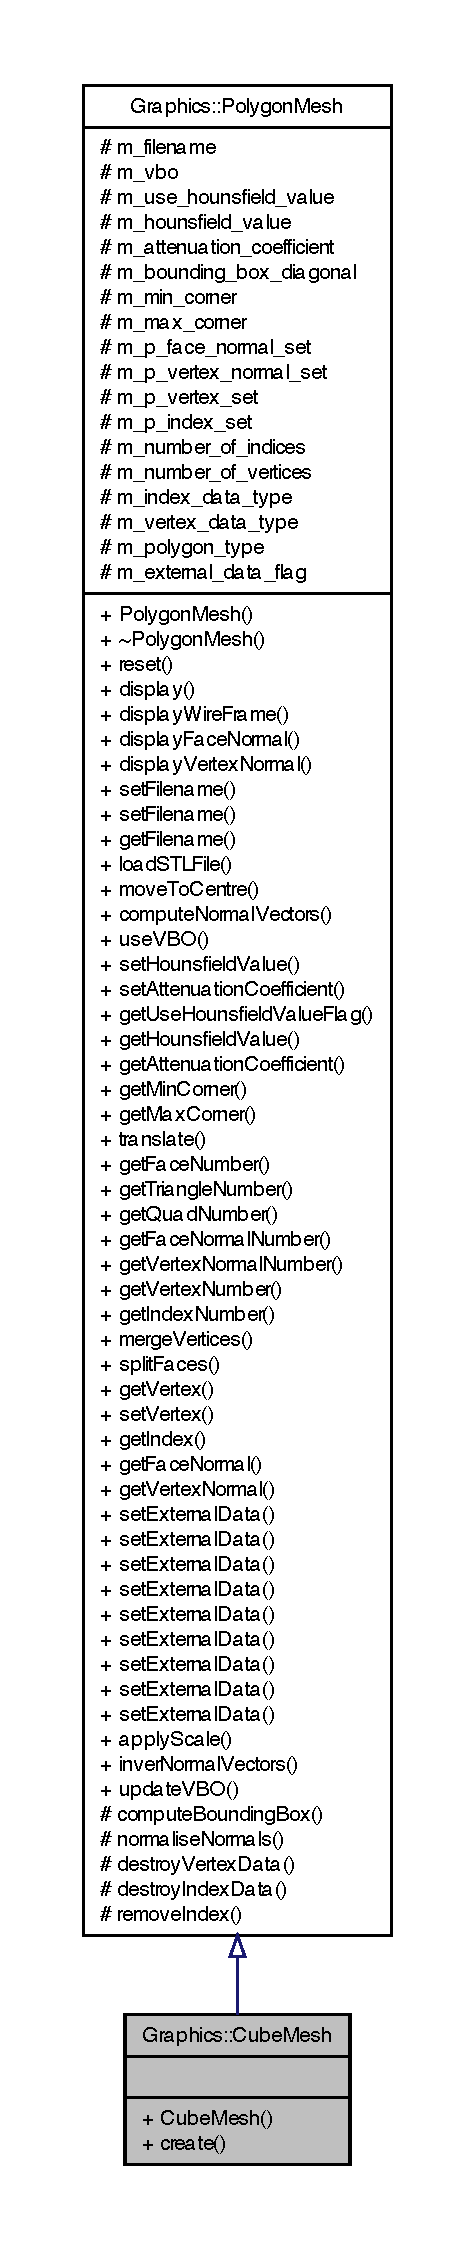
\includegraphics[height=600pt]{class_graphics_1_1_cube_mesh__inherit__graph}
\end{center}
\end{figure}


Collaboration diagram for Graphics::CubeMesh:
\nopagebreak
\begin{figure}[H]
\begin{center}
\leavevmode
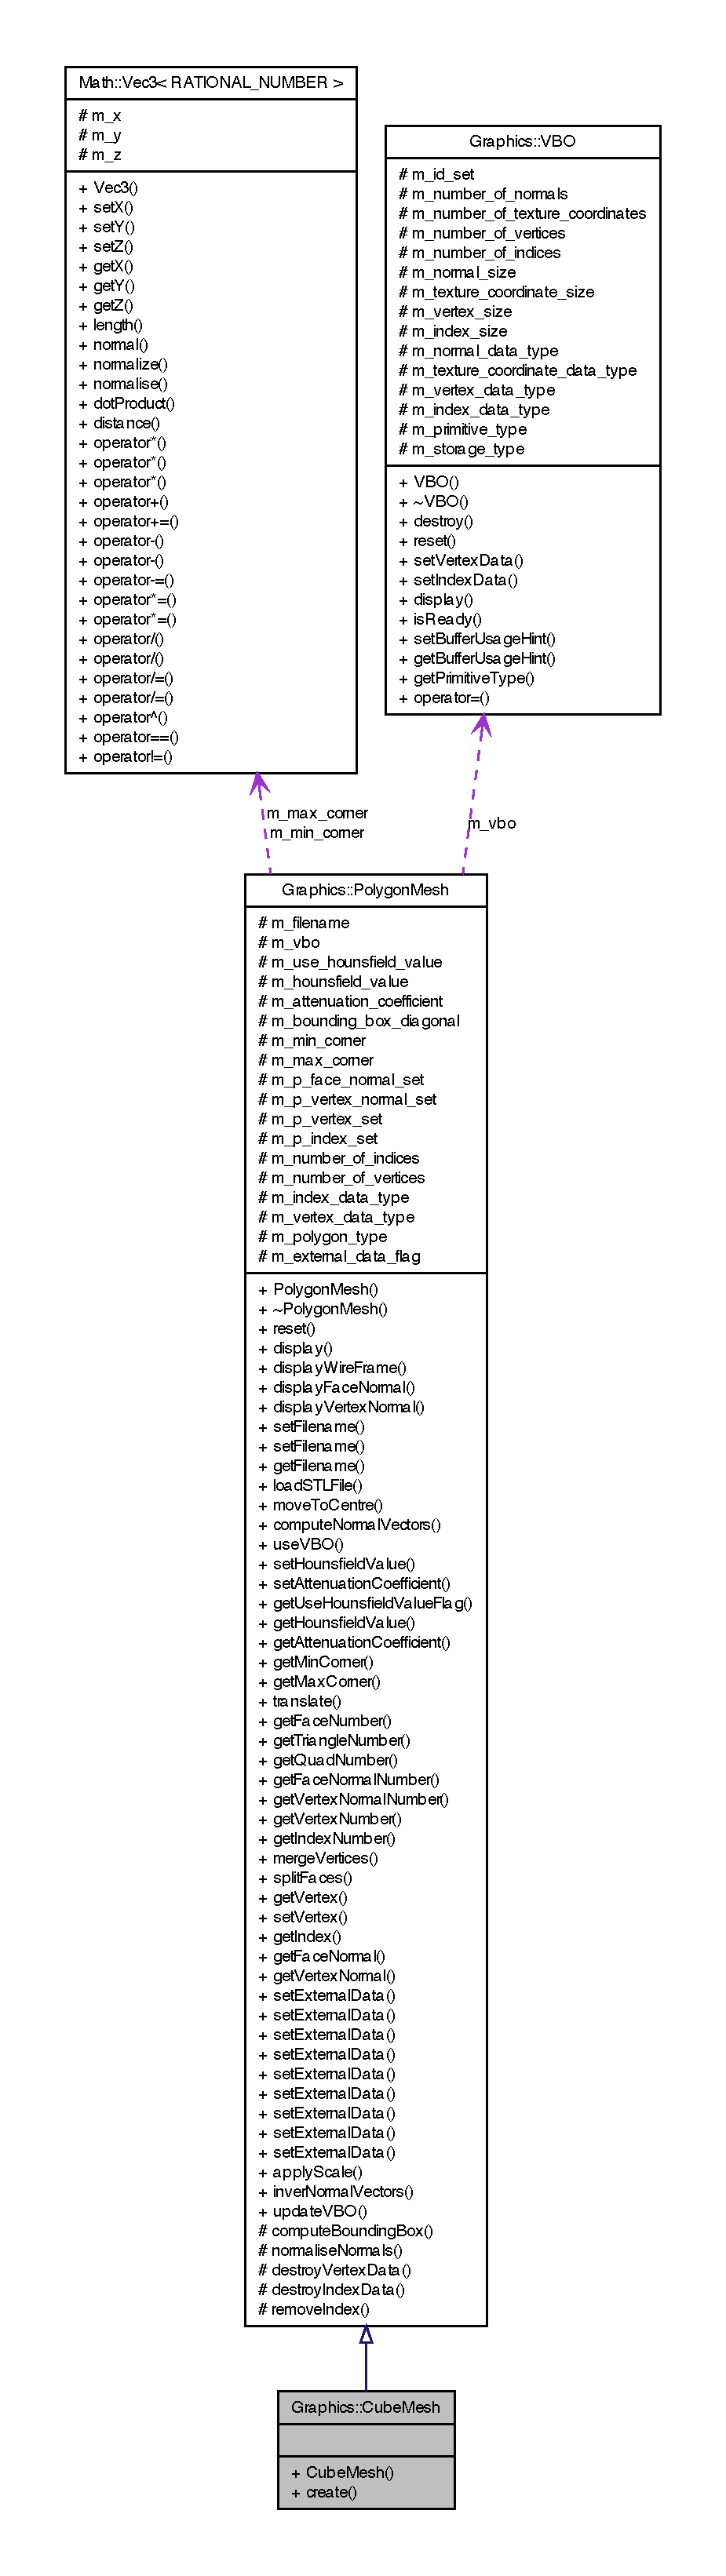
\includegraphics[height=600pt]{class_graphics_1_1_cube_mesh__coll__graph}
\end{center}
\end{figure}
\subsection*{Public Member Functions}
\begin{DoxyCompactItemize}
\item 
\hyperlink{class_graphics_1_1_cube_mesh_a7c2a04863505e9f7d360749a9d1ab755}{CubeMesh} (float aLength=1.0 $\ast$cm)
\begin{DoxyCompactList}\small\item\em Default constructor. \end{DoxyCompactList}\item 
void \hyperlink{class_graphics_1_1_cube_mesh_a5e208101f21490653d4fe4c68bc67464}{create} (float aLength=1.0 $\ast$cm)
\begin{DoxyCompactList}\small\item\em Create a new sphere. \end{DoxyCompactList}\end{DoxyCompactItemize}


\subsection{Detailed Description}
\hyperlink{class_graphics_1_1_cube_mesh}{CubeMesh} is a class to handle 3D meshes of cubes. 

Definition at line 63 of file CubeMesh.h.



\subsection{Constructor \& Destructor Documentation}
\hypertarget{class_graphics_1_1_cube_mesh_a7c2a04863505e9f7d360749a9d1ab755}{
\index{Graphics::CubeMesh@{Graphics::CubeMesh}!CubeMesh@{CubeMesh}}
\index{CubeMesh@{CubeMesh}!Graphics::CubeMesh@{Graphics::CubeMesh}}
\subsubsection[{CubeMesh}]{\setlength{\rightskip}{0pt plus 5cm}Graphics::CubeMesh::CubeMesh (
\begin{DoxyParamCaption}
\item[{float}]{aLength = {\ttfamily 1.0~$\ast$~cm}}
\end{DoxyParamCaption}
)\hspace{0.3cm}{\ttfamily  \mbox{[}inline\mbox{]}}}}
\label{class_graphics_1_1_cube_mesh_a7c2a04863505e9f7d360749a9d1ab755}


Default constructor. 



Definition at line 54 of file CubeMesh.inl.



\subsection{Member Function Documentation}
\hypertarget{class_graphics_1_1_cube_mesh_a5e208101f21490653d4fe4c68bc67464}{
\index{Graphics::CubeMesh@{Graphics::CubeMesh}!create@{create}}
\index{create@{create}!Graphics::CubeMesh@{Graphics::CubeMesh}}
\subsubsection[{create}]{\setlength{\rightskip}{0pt plus 5cm}void Graphics::CubeMesh::create (
\begin{DoxyParamCaption}
\item[{float}]{aLength = {\ttfamily 1.0~$\ast$cm}}
\end{DoxyParamCaption}
)}}
\label{class_graphics_1_1_cube_mesh_a5e208101f21490653d4fe4c68bc67464}


Create a new sphere. 



The documentation for this class was generated from the following files:\begin{DoxyCompactItemize}
\item 
/Users/fpvidal/Documents/gvirtualxray-\/code/trunk/include/gVirtualXRay/\hyperlink{_cube_mesh_8h}{CubeMesh.h}\item 
/Users/fpvidal/Documents/gvirtualxray-\/code/trunk/include/gVirtualXRay/\hyperlink{_cube_mesh_8inl}{CubeMesh.inl}\end{DoxyCompactItemize}

\hypertarget{class_graphics_1_1_implicit_surface_1_1_density_function_parameter_type}{
\section{Graphics::ImplicitSurface::DensityFunctionParameterType Class Reference}
\label{class_graphics_1_1_implicit_surface_1_1_density_function_parameter_type}\index{Graphics::ImplicitSurface::DensityFunctionParameterType@{Graphics::ImplicitSurface::DensityFunctionParameterType}}
}


Type of density function parameter.  




{\ttfamily \#include $<$ImplicitSurface.h$>$}

\subsection*{Public Member Functions}
\begin{DoxyCompactItemize}
\item 
\hyperlink{class_graphics_1_1_implicit_surface_1_1_density_function_parameter_type_ab5bc60b7b3fa2f295a9b0b93d186924c}{DensityFunctionParameterType} (const \hyperlink{class_graphics_1_1_implicit_surface_ab19cb1eb5b21daefd95b6d007be5c199}{DensityFunctionType} aDensityFunctionType=BLOBBY\_\-MOLECULE, \hyperlink{namespace_utilities_a40969b96bd8d847b962e297cb79f08ce}{RATIONAL\_\-NUMBER} a=1, \hyperlink{namespace_utilities_a40969b96bd8d847b962e297cb79f08ce}{RATIONAL\_\-NUMBER} b=1)
\begin{DoxyCompactList}\small\item\em Default constructor. \end{DoxyCompactList}\end{DoxyCompactItemize}
\subsection*{Public Attributes}
\begin{DoxyCompactItemize}
\item 
\hyperlink{class_graphics_1_1_implicit_surface_ab19cb1eb5b21daefd95b6d007be5c199}{DensityFunctionType} \hyperlink{class_graphics_1_1_implicit_surface_1_1_density_function_parameter_type_a44b2e0b74f79d7665577633deb1ab5cc}{m\_\-density\_\-function}
\begin{DoxyCompactList}\small\item\em Type of density function. \end{DoxyCompactList}\item 
\hyperlink{namespace_utilities_a40969b96bd8d847b962e297cb79f08ce}{RATIONAL\_\-NUMBER} \hyperlink{class_graphics_1_1_implicit_surface_1_1_density_function_parameter_type_a723b894e3d93133824d36fc254ce2747}{m\_\-a}
\begin{DoxyCompactList}\small\item\em First parameter of the density function. \end{DoxyCompactList}\item 
\hyperlink{namespace_utilities_a40969b96bd8d847b962e297cb79f08ce}{RATIONAL\_\-NUMBER} \hyperlink{class_graphics_1_1_implicit_surface_1_1_density_function_parameter_type_ac06dddf51ad8733c4e8f54894a9cb64b}{m\_\-b}
\end{DoxyCompactItemize}


\subsection{Detailed Description}
Type of density function parameter. 

Definition at line 86 of file ImplicitSurface.h.



\subsection{Constructor \& Destructor Documentation}
\hypertarget{class_graphics_1_1_implicit_surface_1_1_density_function_parameter_type_ab5bc60b7b3fa2f295a9b0b93d186924c}{
\index{Graphics::ImplicitSurface::DensityFunctionParameterType@{Graphics::ImplicitSurface::DensityFunctionParameterType}!DensityFunctionParameterType@{DensityFunctionParameterType}}
\index{DensityFunctionParameterType@{DensityFunctionParameterType}!Graphics::ImplicitSurface::DensityFunctionParameterType@{Graphics::ImplicitSurface::DensityFunctionParameterType}}
\subsubsection[{DensityFunctionParameterType}]{\setlength{\rightskip}{0pt plus 5cm}Graphics::ImplicitSurface::DensityFunctionParameterType::DensityFunctionParameterType (
\begin{DoxyParamCaption}
\item[{const {\bf DensityFunctionType}}]{aDensityFunctionType = {\ttfamily BLOBBY\_\-MOLECULE}, }
\item[{{\bf RATIONAL\_\-NUMBER}}]{a = {\ttfamily 1}, }
\item[{{\bf RATIONAL\_\-NUMBER}}]{b = {\ttfamily 1}}
\end{DoxyParamCaption}
)\hspace{0.3cm}{\ttfamily  \mbox{[}inline\mbox{]}}}}
\label{class_graphics_1_1_implicit_surface_1_1_density_function_parameter_type_ab5bc60b7b3fa2f295a9b0b93d186924c}


Default constructor. 


\begin{DoxyParams}{Parameters}
{\em aDensityFunctionType,:} & the type of density function (default value: BLOBBY\_\-MOLECULE) \\
\hline
{\em a,:} & the first parameter (default value: 1) \\
\hline
{\em b,:} & the second parameter (default value: 1) \\
\hline
\end{DoxyParams}
\begin{DoxyReturn}{Returns}
the density 
\end{DoxyReturn}


Definition at line 98 of file ImplicitSurface.h.



\subsection{Member Data Documentation}
\hypertarget{class_graphics_1_1_implicit_surface_1_1_density_function_parameter_type_a723b894e3d93133824d36fc254ce2747}{
\index{Graphics::ImplicitSurface::DensityFunctionParameterType@{Graphics::ImplicitSurface::DensityFunctionParameterType}!m\_\-a@{m\_\-a}}
\index{m\_\-a@{m\_\-a}!Graphics::ImplicitSurface::DensityFunctionParameterType@{Graphics::ImplicitSurface::DensityFunctionParameterType}}
\subsubsection[{m\_\-a}]{\setlength{\rightskip}{0pt plus 5cm}{\bf RATIONAL\_\-NUMBER} {\bf Graphics::ImplicitSurface::DensityFunctionParameterType::m\_\-a}}}
\label{class_graphics_1_1_implicit_surface_1_1_density_function_parameter_type_a723b894e3d93133824d36fc254ce2747}


First parameter of the density function. 



Definition at line 112 of file ImplicitSurface.h.

\hypertarget{class_graphics_1_1_implicit_surface_1_1_density_function_parameter_type_ac06dddf51ad8733c4e8f54894a9cb64b}{
\index{Graphics::ImplicitSurface::DensityFunctionParameterType@{Graphics::ImplicitSurface::DensityFunctionParameterType}!m\_\-b@{m\_\-b}}
\index{m\_\-b@{m\_\-b}!Graphics::ImplicitSurface::DensityFunctionParameterType@{Graphics::ImplicitSurface::DensityFunctionParameterType}}
\subsubsection[{m\_\-b}]{\setlength{\rightskip}{0pt plus 5cm}{\bf RATIONAL\_\-NUMBER} {\bf Graphics::ImplicitSurface::DensityFunctionParameterType::m\_\-b}}}
\label{class_graphics_1_1_implicit_surface_1_1_density_function_parameter_type_ac06dddf51ad8733c4e8f54894a9cb64b}
Secnd parameter of the density function (not used if m\_\-density\_\-function is SPHERE) 

Definition at line 117 of file ImplicitSurface.h.

\hypertarget{class_graphics_1_1_implicit_surface_1_1_density_function_parameter_type_a44b2e0b74f79d7665577633deb1ab5cc}{
\index{Graphics::ImplicitSurface::DensityFunctionParameterType@{Graphics::ImplicitSurface::DensityFunctionParameterType}!m\_\-density\_\-function@{m\_\-density\_\-function}}
\index{m\_\-density\_\-function@{m\_\-density\_\-function}!Graphics::ImplicitSurface::DensityFunctionParameterType@{Graphics::ImplicitSurface::DensityFunctionParameterType}}
\subsubsection[{m\_\-density\_\-function}]{\setlength{\rightskip}{0pt plus 5cm}{\bf DensityFunctionType} {\bf Graphics::ImplicitSurface::DensityFunctionParameterType::m\_\-density\_\-function}}}
\label{class_graphics_1_1_implicit_surface_1_1_density_function_parameter_type_a44b2e0b74f79d7665577633deb1ab5cc}


Type of density function. 



Definition at line 108 of file ImplicitSurface.h.



The documentation for this class was generated from the following file:\begin{DoxyCompactItemize}
\item 
/Users/fpvidal/Documents/gvirtualxray-\/code/trunk/include/gVirtualXRay/\hyperlink{_implicit_surface_8h}{ImplicitSurface.h}\end{DoxyCompactItemize}

\hypertarget{class_utilities_1_1_exception}{
\section{Utilities::Exception Class Reference}
\label{class_utilities_1_1_exception}\index{Utilities::Exception@{Utilities::Exception}}
}


\hyperlink{class_utilities_1_1_exception}{Exception} is a class to handle exceptions.  




{\ttfamily \#include $<$Exception.h$>$}



Inheritance diagram for Utilities::Exception:\nopagebreak
\begin{figure}[H]
\begin{center}
\leavevmode
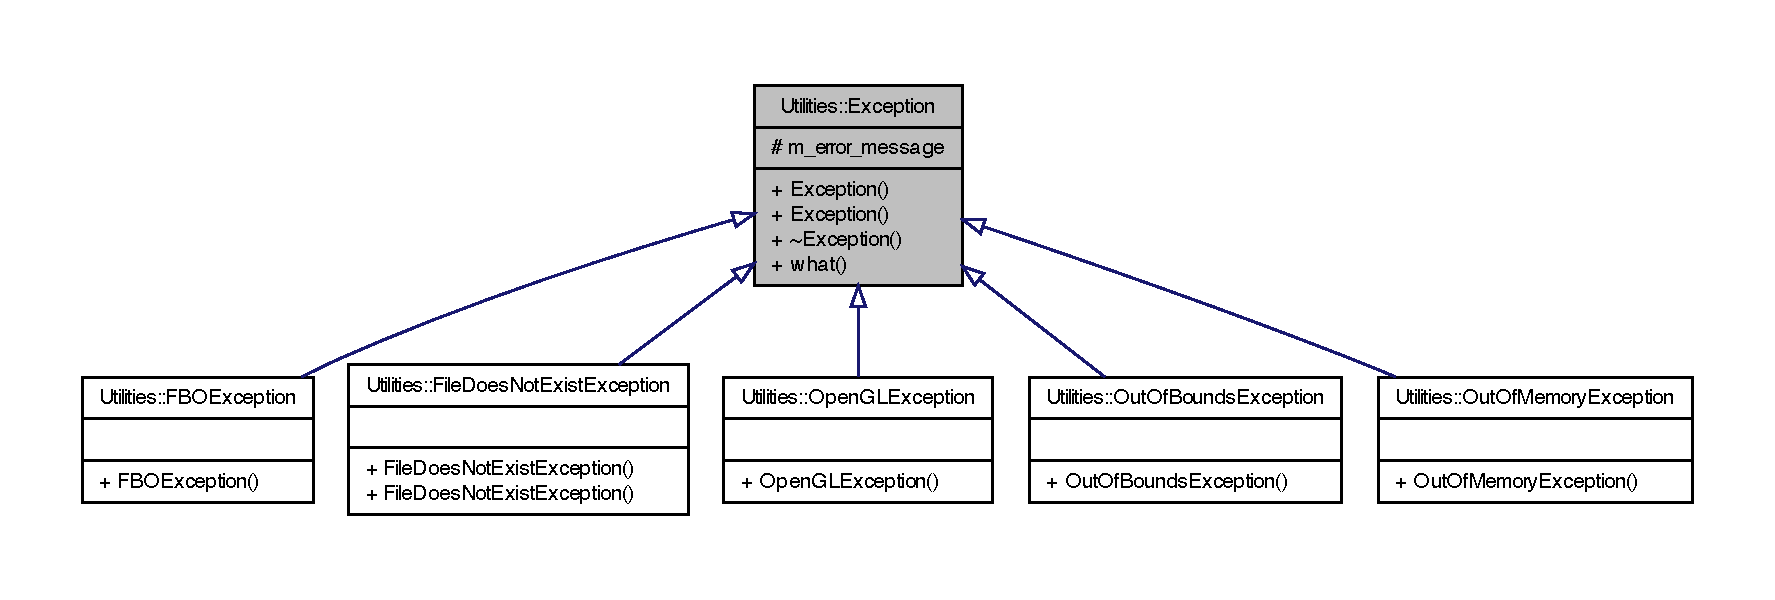
\includegraphics[width=400pt]{class_utilities_1_1_exception__inherit__graph}
\end{center}
\end{figure}
\subsection*{Public Member Functions}
\begin{DoxyCompactItemize}
\item 
\hyperlink{class_utilities_1_1_exception_ac2712b844b42284c9e6b0edb57c4afed}{Exception} (const char $\ast$aFileName=0, const char $\ast$aFunctionName=0, int anErrorLine=0, const char $\ast$anErrorMessage=0)
\begin{DoxyCompactList}\small\item\em Default constructor. \end{DoxyCompactList}\item 
\hyperlink{class_utilities_1_1_exception_a471b083b2db9b08bfd677bec686e8e1d}{Exception} (const char $\ast$aFileName, const char $\ast$aFunctionName, int anErrorLine, const std::string \&anErrorMessage)
\begin{DoxyCompactList}\small\item\em Constructor. \end{DoxyCompactList}\item 
virtual \hyperlink{class_utilities_1_1_exception_ac68e4d053f628a38f087544061d5e5ae}{$\sim$Exception} ()  throw ()
\begin{DoxyCompactList}\small\item\em Destructor. \end{DoxyCompactList}\item 
virtual const char $\ast$ \hyperlink{class_utilities_1_1_exception_a4da7cf325f8b1298ec0251b089151050}{what} () const   throw ()
\begin{DoxyCompactList}\small\item\em Accessor on the error message. \end{DoxyCompactList}\end{DoxyCompactItemize}
\subsection*{Protected Attributes}
\begin{DoxyCompactItemize}
\item 
std::string \hyperlink{class_utilities_1_1_exception_ac7d1b4a0d282072c608059f30c3cba80}{m\_\-error\_\-message}
\begin{DoxyCompactList}\small\item\em The error message. \end{DoxyCompactList}\end{DoxyCompactItemize}


\subsection{Detailed Description}
\hyperlink{class_utilities_1_1_exception}{Exception} is a class to handle exceptions. 

Definition at line 76 of file Exception.h.



\subsection{Constructor \& Destructor Documentation}
\hypertarget{class_utilities_1_1_exception_ac2712b844b42284c9e6b0edb57c4afed}{
\index{Utilities::Exception@{Utilities::Exception}!Exception@{Exception}}
\index{Exception@{Exception}!Utilities::Exception@{Utilities::Exception}}
\subsubsection[{Exception}]{\setlength{\rightskip}{0pt plus 5cm}Utilities::Exception::Exception (
\begin{DoxyParamCaption}
\item[{const char $\ast$}]{aFileName = {\ttfamily 0}, }
\item[{const char $\ast$}]{aFunctionName = {\ttfamily 0}, }
\item[{int}]{anErrorLine = {\ttfamily 0}, }
\item[{const char $\ast$}]{anErrorMessage = {\ttfamily 0}}
\end{DoxyParamCaption}
)\hspace{0.3cm}{\ttfamily  \mbox{[}inline\mbox{]}}}}
\label{class_utilities_1_1_exception_ac2712b844b42284c9e6b0edb57c4afed}


Default constructor. 


\begin{DoxyParams}{Parameters}
{\em aFileName,:} & name of the source file where the exception was thrown (default value: 0) \\
\hline
{\em aFunctionName,:} & name of the function where the exception was thrown (default value: 0) \\
\hline
{\em anErrorLine,:} & name at which the exception was thrown (default value: 0) \\
\hline
{\em anErrorMessage,:} & error message corresponding to the exception (default value: 0) \\
\hline
\end{DoxyParams}


Definition at line 58 of file Exception.inl.

\hypertarget{class_utilities_1_1_exception_a471b083b2db9b08bfd677bec686e8e1d}{
\index{Utilities::Exception@{Utilities::Exception}!Exception@{Exception}}
\index{Exception@{Exception}!Utilities::Exception@{Utilities::Exception}}
\subsubsection[{Exception}]{\setlength{\rightskip}{0pt plus 5cm}Utilities::Exception::Exception (
\begin{DoxyParamCaption}
\item[{const char $\ast$}]{aFileName, }
\item[{const char $\ast$}]{aFunctionName, }
\item[{int}]{anErrorLine, }
\item[{const std::string \&}]{anErrorMessage}
\end{DoxyParamCaption}
)\hspace{0.3cm}{\ttfamily  \mbox{[}inline\mbox{]}}}}
\label{class_utilities_1_1_exception_a471b083b2db9b08bfd677bec686e8e1d}


Constructor. 


\begin{DoxyParams}{Parameters}
{\em aFileName,:} & name of the source file where the exception was thrown (default value: 0) \\
\hline
{\em aFunctionName,:} & name of the function where the exception was thrown (default value: 0) \\
\hline
{\em anErrorLine,:} & name at which the exception was thrown (default value: 0) \\
\hline
{\em anErrorMessage,:} & error message corresponding to the exception (default value: 0) \\
\hline
\end{DoxyParams}


Definition at line 85 of file Exception.inl.

\hypertarget{class_utilities_1_1_exception_ac68e4d053f628a38f087544061d5e5ae}{
\index{Utilities::Exception@{Utilities::Exception}!$\sim$Exception@{$\sim$Exception}}
\index{$\sim$Exception@{$\sim$Exception}!Utilities::Exception@{Utilities::Exception}}
\subsubsection[{$\sim$Exception}]{\setlength{\rightskip}{0pt plus 5cm}Utilities::Exception::$\sim$Exception (
\begin{DoxyParamCaption}
{}
\end{DoxyParamCaption}
)  throw ()\hspace{0.3cm}{\ttfamily  \mbox{[}inline, virtual\mbox{]}}}}
\label{class_utilities_1_1_exception_ac68e4d053f628a38f087544061d5e5ae}


Destructor. 



Definition at line 104 of file Exception.inl.



\subsection{Member Function Documentation}
\hypertarget{class_utilities_1_1_exception_a4da7cf325f8b1298ec0251b089151050}{
\index{Utilities::Exception@{Utilities::Exception}!what@{what}}
\index{what@{what}!Utilities::Exception@{Utilities::Exception}}
\subsubsection[{what}]{\setlength{\rightskip}{0pt plus 5cm}const char $\ast$ Utilities::Exception::what (
\begin{DoxyParamCaption}
{}
\end{DoxyParamCaption}
) const  throw ()\hspace{0.3cm}{\ttfamily  \mbox{[}inline, virtual\mbox{]}}}}
\label{class_utilities_1_1_exception_a4da7cf325f8b1298ec0251b089151050}


Accessor on the error message. 

\begin{DoxyReturn}{Returns}
the error message 
\end{DoxyReturn}


Definition at line 110 of file Exception.inl.



\subsection{Member Data Documentation}
\hypertarget{class_utilities_1_1_exception_ac7d1b4a0d282072c608059f30c3cba80}{
\index{Utilities::Exception@{Utilities::Exception}!m\_\-error\_\-message@{m\_\-error\_\-message}}
\index{m\_\-error\_\-message@{m\_\-error\_\-message}!Utilities::Exception@{Utilities::Exception}}
\subsubsection[{m\_\-error\_\-message}]{\setlength{\rightskip}{0pt plus 5cm}std::string {\bf Utilities::Exception::m\_\-error\_\-message}\hspace{0.3cm}{\ttfamily  \mbox{[}protected\mbox{]}}}}
\label{class_utilities_1_1_exception_ac7d1b4a0d282072c608059f30c3cba80}


The error message. 



Definition at line 123 of file Exception.h.



The documentation for this class was generated from the following files:\begin{DoxyCompactItemize}
\item 
/Users/fpvidal/Documents/gvirtualxray-\/code/trunk/include/gVirtualXRay/\hyperlink{_exception_8h}{Exception.h}\item 
/Users/fpvidal/Documents/gvirtualxray-\/code/trunk/include/gVirtualXRay/\hyperlink{_exception_8inl}{Exception.inl}\end{DoxyCompactItemize}

\hypertarget{class_utilities_1_1_f_b_o_exception}{
\section{Utilities::FBOException Class Reference}
\label{class_utilities_1_1_f_b_o_exception}\index{Utilities::FBOException@{Utilities::FBOException}}
}


\hyperlink{class_utilities_1_1_f_b_o_exception}{FBOException} is a class to handle exceptions related to FBOs.  




{\ttfamily \#include $<$FBOException.h$>$}



Inheritance diagram for Utilities::FBOException:\nopagebreak
\begin{figure}[H]
\begin{center}
\leavevmode
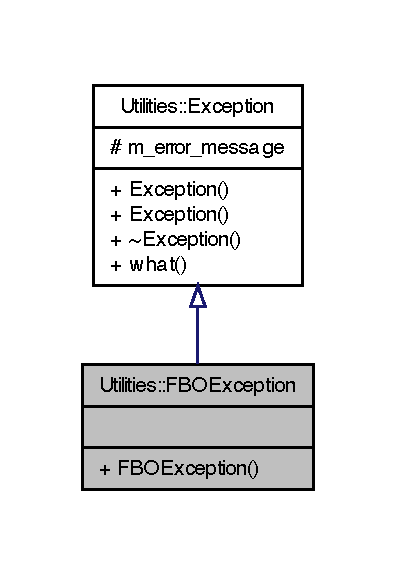
\includegraphics[width=190pt]{class_utilities_1_1_f_b_o_exception__inherit__graph}
\end{center}
\end{figure}


Collaboration diagram for Utilities::FBOException:\nopagebreak
\begin{figure}[H]
\begin{center}
\leavevmode
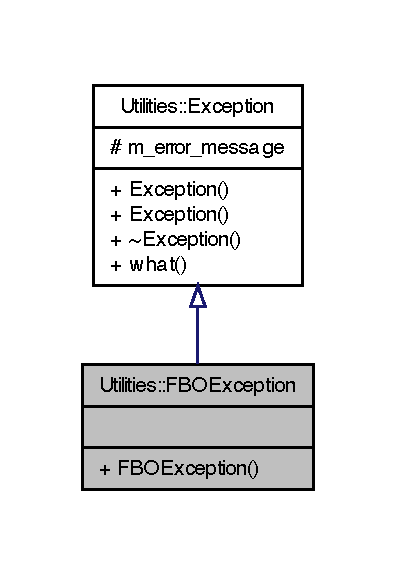
\includegraphics[width=190pt]{class_utilities_1_1_f_b_o_exception__coll__graph}
\end{center}
\end{figure}
\subsection*{Public Member Functions}
\begin{DoxyCompactItemize}
\item 
\hyperlink{class_utilities_1_1_f_b_o_exception_a5acdd259391453a319113f7e4cfd9386}{FBOException} (const char $\ast$aFileName, const char $\ast$aFunctionName, int anErrorLine, int anErrorCode)
\begin{DoxyCompactList}\small\item\em Default constructor. \end{DoxyCompactList}\end{DoxyCompactItemize}


\subsection{Detailed Description}
\hyperlink{class_utilities_1_1_f_b_o_exception}{FBOException} is a class to handle exceptions related to FBOs. 

Definition at line 53 of file FBOException.h.



\subsection{Constructor \& Destructor Documentation}
\hypertarget{class_utilities_1_1_f_b_o_exception_a5acdd259391453a319113f7e4cfd9386}{
\index{Utilities::FBOException@{Utilities::FBOException}!FBOException@{FBOException}}
\index{FBOException@{FBOException}!Utilities::FBOException@{Utilities::FBOException}}
\subsubsection[{FBOException}]{\setlength{\rightskip}{0pt plus 5cm}Utilities::FBOException::FBOException (
\begin{DoxyParamCaption}
\item[{const char $\ast$}]{aFileName, }
\item[{const char $\ast$}]{aFunctionName, }
\item[{int}]{anErrorLine, }
\item[{int}]{anErrorCode}
\end{DoxyParamCaption}
)}}
\label{class_utilities_1_1_f_b_o_exception_a5acdd259391453a319113f7e4cfd9386}


Default constructor. 


\begin{DoxyParams}{Parameters}
{\em aFileName,:} & name of the source file where the exception was thrown \\
\hline
{\em aFunctionName,:} & name of the function where the exception was thrown \\
\hline
{\em anErrorLine,:} & name at which the exception was thrown \\
\hline
{\em anErrorCode,:} & FBO error code \\
\hline
\end{DoxyParams}


The documentation for this class was generated from the following file:\begin{DoxyCompactItemize}
\item 
/Users/fpvidal/Documents/gvirtualxray-\/code/trunk/include/gVirtualXRay/\hyperlink{_f_b_o_exception_8h}{FBOException.h}\end{DoxyCompactItemize}

\hypertarget{class_utilities_1_1_file_does_not_exist_exception}{
\section{Utilities::FileDoesNotExistException Class Reference}
\label{class_utilities_1_1_file_does_not_exist_exception}\index{Utilities::FileDoesNotExistException@{Utilities::FileDoesNotExistException}}
}


\hyperlink{class_utilities_1_1_file_does_not_exist_exception}{FileDoesNotExistException} is a class to handle exceptions when trying to open a read-\/only file that is not accessible.  




{\ttfamily \#include $<$FileDoesNotExistException.h$>$}



Inheritance diagram for Utilities::FileDoesNotExistException:\nopagebreak
\begin{figure}[H]
\begin{center}
\leavevmode
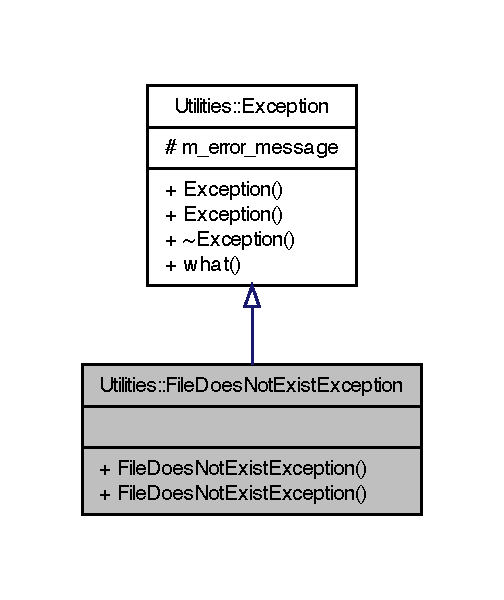
\includegraphics[width=242pt]{class_utilities_1_1_file_does_not_exist_exception__inherit__graph}
\end{center}
\end{figure}


Collaboration diagram for Utilities::FileDoesNotExistException:\nopagebreak
\begin{figure}[H]
\begin{center}
\leavevmode
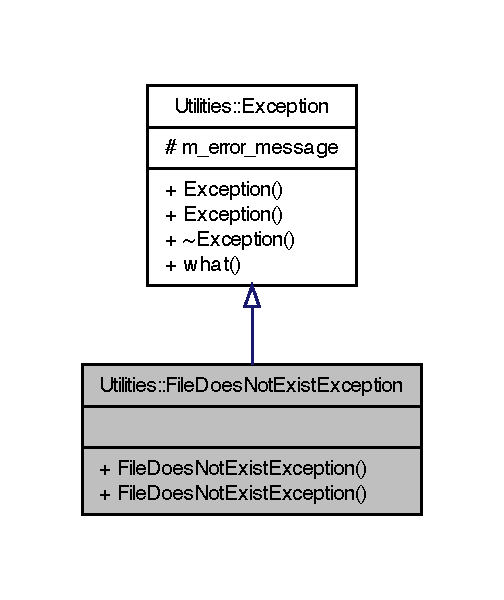
\includegraphics[width=242pt]{class_utilities_1_1_file_does_not_exist_exception__coll__graph}
\end{center}
\end{figure}
\subsection*{Public Member Functions}
\begin{DoxyCompactItemize}
\item 
\hyperlink{class_utilities_1_1_file_does_not_exist_exception_a3f0123531651805b52432f0d34f06b90}{FileDoesNotExistException} (const char $\ast$aFileName, const char $\ast$aFunctionName, int anErrorLine, const char $\ast$aNameOfFileToOpen)
\begin{DoxyCompactList}\small\item\em Constructor. \end{DoxyCompactList}\item 
\hyperlink{class_utilities_1_1_file_does_not_exist_exception_ab2faca6a36eabaff1e2fdd8df2731fb2}{FileDoesNotExistException} (const char $\ast$aFileName, const char $\ast$aFunctionName, int anErrorLine, const std::string \&aNameOfFileToOpen)
\begin{DoxyCompactList}\small\item\em Constructor. \end{DoxyCompactList}\end{DoxyCompactItemize}


\subsection{Detailed Description}
\hyperlink{class_utilities_1_1_file_does_not_exist_exception}{FileDoesNotExistException} is a class to handle exceptions when trying to open a read-\/only file that is not accessible. 

Definition at line 57 of file FileDoesNotExistException.h.



\subsection{Constructor \& Destructor Documentation}
\hypertarget{class_utilities_1_1_file_does_not_exist_exception_a3f0123531651805b52432f0d34f06b90}{
\index{Utilities::FileDoesNotExistException@{Utilities::FileDoesNotExistException}!FileDoesNotExistException@{FileDoesNotExistException}}
\index{FileDoesNotExistException@{FileDoesNotExistException}!Utilities::FileDoesNotExistException@{Utilities::FileDoesNotExistException}}
\subsubsection[{FileDoesNotExistException}]{\setlength{\rightskip}{0pt plus 5cm}Utilities::FileDoesNotExistException::FileDoesNotExistException (
\begin{DoxyParamCaption}
\item[{const char $\ast$}]{aFileName, }
\item[{const char $\ast$}]{aFunctionName, }
\item[{int}]{anErrorLine, }
\item[{const char $\ast$}]{aNameOfFileToOpen}
\end{DoxyParamCaption}
)\hspace{0.3cm}{\ttfamily  \mbox{[}inline\mbox{]}}}}
\label{class_utilities_1_1_file_does_not_exist_exception_a3f0123531651805b52432f0d34f06b90}


Constructor. 


\begin{DoxyParams}{Parameters}
{\em aFileName,:} & name of the source file where the exception was thrown \\
\hline
{\em aFunctionName,:} & name of the function where the exception was thrown \\
\hline
{\em anErrorLine,:} & name at which the exception was thrown \\
\hline
{\em aNameOfFileToOpen,:} & the name of the file to open \\
\hline
\end{DoxyParams}


Definition at line 43 of file FileDoesNotExistException.inl.

\hypertarget{class_utilities_1_1_file_does_not_exist_exception_ab2faca6a36eabaff1e2fdd8df2731fb2}{
\index{Utilities::FileDoesNotExistException@{Utilities::FileDoesNotExistException}!FileDoesNotExistException@{FileDoesNotExistException}}
\index{FileDoesNotExistException@{FileDoesNotExistException}!Utilities::FileDoesNotExistException@{Utilities::FileDoesNotExistException}}
\subsubsection[{FileDoesNotExistException}]{\setlength{\rightskip}{0pt plus 5cm}Utilities::FileDoesNotExistException::FileDoesNotExistException (
\begin{DoxyParamCaption}
\item[{const char $\ast$}]{aFileName, }
\item[{const char $\ast$}]{aFunctionName, }
\item[{int}]{anErrorLine, }
\item[{const std::string \&}]{aNameOfFileToOpen}
\end{DoxyParamCaption}
)\hspace{0.3cm}{\ttfamily  \mbox{[}inline\mbox{]}}}}
\label{class_utilities_1_1_file_does_not_exist_exception_ab2faca6a36eabaff1e2fdd8df2731fb2}


Constructor. 


\begin{DoxyParams}{Parameters}
{\em aFileName,:} & name of the source file where the exception was thrown \\
\hline
{\em aFunctionName,:} & name of the function where the exception was thrown \\
\hline
{\em anErrorLine,:} & name at which the exception was thrown \\
\hline
{\em aNameOfFileToOpen,:} & the name of the file to open \\
\hline
\end{DoxyParams}


Definition at line 62 of file FileDoesNotExistException.inl.



The documentation for this class was generated from the following files:\begin{DoxyCompactItemize}
\item 
/Users/fpvidal/Documents/gvirtualxray-\/code/trunk/include/gVirtualXRay/\hyperlink{_file_does_not_exist_exception_8h}{FileDoesNotExistException.h}\item 
/Users/fpvidal/Documents/gvirtualxray-\/code/trunk/include/gVirtualXRay/\hyperlink{_file_does_not_exist_exception_8inl}{FileDoesNotExistException.inl}\end{DoxyCompactItemize}

\hypertarget{class_framebuffer_object}{
\section{FramebufferObject Class Reference}
\label{class_framebuffer_object}\index{FramebufferObject@{FramebufferObject}}
}


{\ttfamily \#include $<$framebufferObject.h$>$}

\subsection*{Public Member Functions}
\begin{DoxyCompactItemize}
\item 
\hyperlink{class_framebuffer_object_ad49fee576a90d0a23ac7af93d82d5bbf}{FramebufferObject} ()
\begin{DoxyCompactList}\small\item\em Ctor/Dtor. \end{DoxyCompactList}\item 
virtual \hyperlink{class_framebuffer_object_ae7c58315d303776dc3e14832fe675abb}{$\sim$FramebufferObject} ()
\item 
void \hyperlink{class_framebuffer_object_a1916acbbe9aafb8302dc117a7cce6fcd}{Bind} ()
\begin{DoxyCompactList}\small\item\em Bind this FBO as current render target. \end{DoxyCompactList}\item 
virtual void \hyperlink{class_framebuffer_object_a5c7418c7b49f7a4b56c0575adb9a09a8}{AttachTexture} (GLenum texTarget, GLuint texId, GLenum attachment=GL\_\-COLOR\_\-ATTACHMENT0\_\-EXT, int mipLevel=0, int zSlice=0)
\begin{DoxyCompactList}\small\item\em Bind a texture to the \char`\"{}attachment\char`\"{} point of this FBO. \end{DoxyCompactList}\item 
virtual void \hyperlink{class_framebuffer_object_af83643f5ea3bfedd8c17c8db9f2d8e64}{AttachTextures} (int numTextures, GLenum texTarget\mbox{[}$\,$\mbox{]}, GLuint texId\mbox{[}$\,$\mbox{]}, GLenum attachment\mbox{[}$\,$\mbox{]}=NULL, int mipLevel\mbox{[}$\,$\mbox{]}=NULL, int zSlice\mbox{[}$\,$\mbox{]}=NULL)
\item 
virtual void \hyperlink{class_framebuffer_object_ad6af74957e36f61102d492fa6a5908f5}{AttachRenderBuffer} (GLuint buffId, GLenum attachment=GL\_\-COLOR\_\-ATTACHMENT0\_\-EXT)
\begin{DoxyCompactList}\small\item\em Bind a render buffer to the \char`\"{}attachment\char`\"{} point of this FBO. \end{DoxyCompactList}\item 
virtual void \hyperlink{class_framebuffer_object_a6e544bc8b8cbd2775fc9831ee854e4e3}{AttachRenderBuffers} (int numBuffers, GLuint buffId\mbox{[}$\,$\mbox{]}, GLenum attachment\mbox{[}$\,$\mbox{]}=NULL)
\item 
void \hyperlink{class_framebuffer_object_ae37b27bc48c8271e43a89fa94b6ad7c7}{Unattach} (GLenum attachment)
\begin{DoxyCompactList}\small\item\em Free any resource bound to the \char`\"{}attachment\char`\"{} point of this FBO. \end{DoxyCompactList}\item 
void \hyperlink{class_framebuffer_object_a45d0bbcbf43e0f97e93d290ddb275885}{UnattachAll} ()
\begin{DoxyCompactList}\small\item\em Free any resources bound to any attachment points of this FBO. \end{DoxyCompactList}\item 
bool \hyperlink{class_framebuffer_object_ac2b9348526bb9ba9d4c66473bbd7a06b}{IsValid} (std::ostream \&ostr=std::cerr)
\item 
GLenum \hyperlink{class_framebuffer_object_af6eed9070b6fe04cba7535782e54b175}{GetAttachedType} (GLenum attachment)
\begin{DoxyCompactList}\small\item\em Is attached type GL\_\-RENDERBUFFER\_\-EXT or GL\_\-TEXTURE? \end{DoxyCompactList}\item 
GLuint \hyperlink{class_framebuffer_object_a5ed03e1d45321b92a264ab1a91d78f38}{GetAttachedId} (GLenum attachment)
\item 
GLint \hyperlink{class_framebuffer_object_a6572be6d2c59a8b8fb6f3fec126f4480}{GetAttachedMipLevel} (GLenum attachment)
\begin{DoxyCompactList}\small\item\em Which mipmap level is currently attached to \char`\"{}attachement?\char`\"{}. \end{DoxyCompactList}\item 
GLint \hyperlink{class_framebuffer_object_af7fe7616b07381b294eac1ae3d6df2fa}{GetAttachedCubeFace} (GLenum attachment)
\begin{DoxyCompactList}\small\item\em Which cube face is currently attached to \char`\"{}attachment?\char`\"{}. \end{DoxyCompactList}\item 
GLint \hyperlink{class_framebuffer_object_a386de725cd22b3f4f75692c653e0ac86}{GetAttachedZSlice} (GLenum attachment)
\begin{DoxyCompactList}\small\item\em Which z-\/slice is currently attached to \char`\"{}attachment?\char`\"{}. \end{DoxyCompactList}\end{DoxyCompactItemize}
\subsection*{Static Public Member Functions}
\begin{DoxyCompactItemize}
\item 
static int \hyperlink{class_framebuffer_object_ad4c7199850737c4a62b16f102641006d}{GetMaxColorAttachments} ()
\begin{DoxyCompactList}\small\item\em END : Accessors. \end{DoxyCompactList}\item 
static void \hyperlink{class_framebuffer_object_ae327450680f21e18893c3657b8635bf3}{Disable} ()
\end{DoxyCompactItemize}
\subsection*{Protected Member Functions}
\begin{DoxyCompactItemize}
\item 
void \hyperlink{class_framebuffer_object_a98dedda4a464b389da7bf922d9a1f177}{\_\-GuardedBind} ()
\begin{DoxyCompactList}\small\item\em END : Static methods global to all FBOs. \end{DoxyCompactList}\item 
void \hyperlink{class_framebuffer_object_a3935a7e0d87eab285cb667103fbb7b4d}{\_\-GuardedUnbind} ()
\item 
void \hyperlink{class_framebuffer_object_a22cbada4c9d986edf1044bbb72c18959}{\_\-FramebufferTextureND} (GLenum attachment, GLenum texTarget, GLuint texId, int mipLevel, int zSlice)
\end{DoxyCompactItemize}
\subsection*{Static Protected Member Functions}
\begin{DoxyCompactItemize}
\item 
static GLuint \hyperlink{class_framebuffer_object_a06e52f50f7a54fd8047d49cb4d93d6a7}{\_\-GenerateFboId} ()
\end{DoxyCompactItemize}


\subsection{Detailed Description}
\hyperlink{class_framebuffer_object}{FramebufferObject} Class. This class encapsulates the \hyperlink{class_framebuffer_object}{FramebufferObject} (FBO) OpenGL spec. See the official spec at: \href{http://oss.sgi.com/projects/ogl-sample/registry/EXT/framebuffer_object.txt}{\tt http://oss.sgi.com/projects/ogl-\/sample/registry/EXT/framebuffer\_\-object.txt}

for details.

A framebuffer object (FBO) is conceptually a structure containing pointers to GPU memory. The memory pointed to is either an OpenGL texture or an OpenGL RenderBuffer. FBOs can be used to render to one or more textures, share depth buffers between multiple sets of color buffers/textures and are a complete replacement for pbuffers.

Performance Notes: 1) It is more efficient (but not required) to call \hyperlink{class_framebuffer_object_a1916acbbe9aafb8302dc117a7cce6fcd}{Bind()} on an FBO before making multiple method calls. For example:

\hyperlink{class_framebuffer_object}{FramebufferObject} fbo; fbo.Bind(); fbo.AttachTexture(GL\_\-TEXTURE\_\-2D, texId0, GL\_\-COLOR\_\-ATTACHMENT0\_\-EXT); fbo.AttachTexture(GL\_\-TEXTURE\_\-2D, texId1, GL\_\-COLOR\_\-ATTACHMENT1\_\-EXT); fbo.IsValid();

To provide a complete encapsulation, the following usage pattern works correctly but is less efficient:

\hyperlink{class_framebuffer_object}{FramebufferObject} fbo; NOTE : No \hyperlink{class_framebuffer_object_a1916acbbe9aafb8302dc117a7cce6fcd}{Bind()} call fbo.AttachTexture(GL\_\-TEXTURE\_\-2D, texId0, GL\_\-COLOR\_\-ATTACHMENT0\_\-EXT); fbo.AttachTexture(GL\_\-TEXTURE\_\-2D, texId1, GL\_\-COLOR\_\-ATTACHMENT1\_\-EXT); fbo.IsValid();

The first usage pattern binds the FBO only once, whereas the second usage binds/unbinds the FBO for each method call.

2) Use \hyperlink{class_framebuffer_object_ae327450680f21e18893c3657b8635bf3}{FramebufferObject::Disable()} sparingly. We have intentionally left out an \char`\"{}Unbind()\char`\"{} method because it is largely unnecessary and encourages rendundant Bind/Unbind coding. Binding an FBO is usually much faster than enabling/disabling a pbuffer, but is still a costly operation. When switching between multiple FBOs and a visible OpenGL framebuffer, the following usage pattern is recommended:

\hyperlink{class_framebuffer_object}{FramebufferObject} fbo1, fbo2; fbo1.Bind(); ... Render ... NOTE : No Unbind/Disable here...

fbo2.Bind(); ... Render ...

Disable FBO rendering and return to visible window OpenGL framebuffer. \hyperlink{class_framebuffer_object_ae327450680f21e18893c3657b8635bf3}{FramebufferObject::Disable()}; 

Definition at line 103 of file framebufferObject.h.



\subsection{Constructor \& Destructor Documentation}
\hypertarget{class_framebuffer_object_ad49fee576a90d0a23ac7af93d82d5bbf}{
\index{FramebufferObject@{FramebufferObject}!FramebufferObject@{FramebufferObject}}
\index{FramebufferObject@{FramebufferObject}!FramebufferObject@{FramebufferObject}}
\subsubsection[{FramebufferObject}]{\setlength{\rightskip}{0pt plus 5cm}FramebufferObject::FramebufferObject (
\begin{DoxyParamCaption}
{}
\end{DoxyParamCaption}
)}}
\label{class_framebuffer_object_ad49fee576a90d0a23ac7af93d82d5bbf}


Ctor/Dtor. 

\hypertarget{class_framebuffer_object_ae7c58315d303776dc3e14832fe675abb}{
\index{FramebufferObject@{FramebufferObject}!$\sim$FramebufferObject@{$\sim$FramebufferObject}}
\index{$\sim$FramebufferObject@{$\sim$FramebufferObject}!FramebufferObject@{FramebufferObject}}
\subsubsection[{$\sim$FramebufferObject}]{\setlength{\rightskip}{0pt plus 5cm}virtual FramebufferObject::$\sim$FramebufferObject (
\begin{DoxyParamCaption}
{}
\end{DoxyParamCaption}
)\hspace{0.3cm}{\ttfamily  \mbox{[}virtual\mbox{]}}}}
\label{class_framebuffer_object_ae7c58315d303776dc3e14832fe675abb}


\subsection{Member Function Documentation}
\hypertarget{class_framebuffer_object_a22cbada4c9d986edf1044bbb72c18959}{
\index{FramebufferObject@{FramebufferObject}!\_\-FramebufferTextureND@{\_\-FramebufferTextureND}}
\index{\_\-FramebufferTextureND@{\_\-FramebufferTextureND}!FramebufferObject@{FramebufferObject}}
\subsubsection[{\_\-FramebufferTextureND}]{\setlength{\rightskip}{0pt plus 5cm}void FramebufferObject::\_\-FramebufferTextureND (
\begin{DoxyParamCaption}
\item[{GLenum}]{attachment, }
\item[{GLenum}]{texTarget, }
\item[{GLuint}]{texId, }
\item[{int}]{mipLevel, }
\item[{int}]{zSlice}
\end{DoxyParamCaption}
)\hspace{0.3cm}{\ttfamily  \mbox{[}protected\mbox{]}}}}
\label{class_framebuffer_object_a22cbada4c9d986edf1044bbb72c18959}
\hypertarget{class_framebuffer_object_a06e52f50f7a54fd8047d49cb4d93d6a7}{
\index{FramebufferObject@{FramebufferObject}!\_\-GenerateFboId@{\_\-GenerateFboId}}
\index{\_\-GenerateFboId@{\_\-GenerateFboId}!FramebufferObject@{FramebufferObject}}
\subsubsection[{\_\-GenerateFboId}]{\setlength{\rightskip}{0pt plus 5cm}static GLuint FramebufferObject::\_\-GenerateFboId (
\begin{DoxyParamCaption}
{}
\end{DoxyParamCaption}
)\hspace{0.3cm}{\ttfamily  \mbox{[}static, protected\mbox{]}}}}
\label{class_framebuffer_object_a06e52f50f7a54fd8047d49cb4d93d6a7}
\hypertarget{class_framebuffer_object_a98dedda4a464b389da7bf922d9a1f177}{
\index{FramebufferObject@{FramebufferObject}!\_\-GuardedBind@{\_\-GuardedBind}}
\index{\_\-GuardedBind@{\_\-GuardedBind}!FramebufferObject@{FramebufferObject}}
\subsubsection[{\_\-GuardedBind}]{\setlength{\rightskip}{0pt plus 5cm}void FramebufferObject::\_\-GuardedBind (
\begin{DoxyParamCaption}
{}
\end{DoxyParamCaption}
)\hspace{0.3cm}{\ttfamily  \mbox{[}protected\mbox{]}}}}
\label{class_framebuffer_object_a98dedda4a464b389da7bf922d9a1f177}


END : Static methods global to all FBOs. 

\hypertarget{class_framebuffer_object_a3935a7e0d87eab285cb667103fbb7b4d}{
\index{FramebufferObject@{FramebufferObject}!\_\-GuardedUnbind@{\_\-GuardedUnbind}}
\index{\_\-GuardedUnbind@{\_\-GuardedUnbind}!FramebufferObject@{FramebufferObject}}
\subsubsection[{\_\-GuardedUnbind}]{\setlength{\rightskip}{0pt plus 5cm}void FramebufferObject::\_\-GuardedUnbind (
\begin{DoxyParamCaption}
{}
\end{DoxyParamCaption}
)\hspace{0.3cm}{\ttfamily  \mbox{[}protected\mbox{]}}}}
\label{class_framebuffer_object_a3935a7e0d87eab285cb667103fbb7b4d}
\hypertarget{class_framebuffer_object_ad6af74957e36f61102d492fa6a5908f5}{
\index{FramebufferObject@{FramebufferObject}!AttachRenderBuffer@{AttachRenderBuffer}}
\index{AttachRenderBuffer@{AttachRenderBuffer}!FramebufferObject@{FramebufferObject}}
\subsubsection[{AttachRenderBuffer}]{\setlength{\rightskip}{0pt plus 5cm}virtual void FramebufferObject::AttachRenderBuffer (
\begin{DoxyParamCaption}
\item[{GLuint}]{buffId, }
\item[{GLenum}]{attachment = {\ttfamily GL\_\-COLOR\_\-ATTACHMENT0\_\-EXT}}
\end{DoxyParamCaption}
)\hspace{0.3cm}{\ttfamily  \mbox{[}virtual\mbox{]}}}}
\label{class_framebuffer_object_ad6af74957e36f61102d492fa6a5908f5}


Bind a render buffer to the \char`\"{}attachment\char`\"{} point of this FBO. 

\hypertarget{class_framebuffer_object_a6e544bc8b8cbd2775fc9831ee854e4e3}{
\index{FramebufferObject@{FramebufferObject}!AttachRenderBuffers@{AttachRenderBuffers}}
\index{AttachRenderBuffers@{AttachRenderBuffers}!FramebufferObject@{FramebufferObject}}
\subsubsection[{AttachRenderBuffers}]{\setlength{\rightskip}{0pt plus 5cm}virtual void FramebufferObject::AttachRenderBuffers (
\begin{DoxyParamCaption}
\item[{int}]{numBuffers, }
\item[{GLuint}]{buffId\mbox{[}$\,$\mbox{]}, }
\item[{GLenum}]{attachment\mbox{[}$\,$\mbox{]} = {\ttfamily NULL}}
\end{DoxyParamCaption}
)\hspace{0.3cm}{\ttfamily  \mbox{[}virtual\mbox{]}}}}
\label{class_framebuffer_object_a6e544bc8b8cbd2775fc9831ee854e4e3}
Bind an array of render buffers to corresponding \char`\"{}attachment\char`\"{} points of this FBO.
\begin{DoxyItemize}
\item By default, the first 'numBuffers' attachments are used, starting with GL\_\-COLOR\_\-ATTACHMENT0\_\-EXT 
\end{DoxyItemize}\hypertarget{class_framebuffer_object_a5c7418c7b49f7a4b56c0575adb9a09a8}{
\index{FramebufferObject@{FramebufferObject}!AttachTexture@{AttachTexture}}
\index{AttachTexture@{AttachTexture}!FramebufferObject@{FramebufferObject}}
\subsubsection[{AttachTexture}]{\setlength{\rightskip}{0pt plus 5cm}virtual void FramebufferObject::AttachTexture (
\begin{DoxyParamCaption}
\item[{GLenum}]{texTarget, }
\item[{GLuint}]{texId, }
\item[{GLenum}]{attachment = {\ttfamily GL\_\-COLOR\_\-ATTACHMENT0\_\-EXT}, }
\item[{int}]{mipLevel = {\ttfamily 0}, }
\item[{int}]{zSlice = {\ttfamily 0}}
\end{DoxyParamCaption}
)\hspace{0.3cm}{\ttfamily  \mbox{[}virtual\mbox{]}}}}
\label{class_framebuffer_object_a5c7418c7b49f7a4b56c0575adb9a09a8}


Bind a texture to the \char`\"{}attachment\char`\"{} point of this FBO. 

\hypertarget{class_framebuffer_object_af83643f5ea3bfedd8c17c8db9f2d8e64}{
\index{FramebufferObject@{FramebufferObject}!AttachTextures@{AttachTextures}}
\index{AttachTextures@{AttachTextures}!FramebufferObject@{FramebufferObject}}
\subsubsection[{AttachTextures}]{\setlength{\rightskip}{0pt plus 5cm}virtual void FramebufferObject::AttachTextures (
\begin{DoxyParamCaption}
\item[{int}]{numTextures, }
\item[{GLenum}]{texTarget\mbox{[}$\,$\mbox{]}, }
\item[{GLuint}]{texId\mbox{[}$\,$\mbox{]}, }
\item[{GLenum}]{attachment\mbox{[}$\,$\mbox{]} = {\ttfamily NULL}, }
\item[{int}]{mipLevel\mbox{[}$\,$\mbox{]} = {\ttfamily NULL}, }
\item[{int}]{zSlice\mbox{[}$\,$\mbox{]} = {\ttfamily NULL}}
\end{DoxyParamCaption}
)\hspace{0.3cm}{\ttfamily  \mbox{[}virtual\mbox{]}}}}
\label{class_framebuffer_object_af83643f5ea3bfedd8c17c8db9f2d8e64}
Bind an array of textures to multiple \char`\"{}attachment\char`\"{} points of this FBO
\begin{DoxyItemize}
\item By default, the first 'numTextures' attachments are used, starting with GL\_\-COLOR\_\-ATTACHMENT0\_\-EXT 
\end{DoxyItemize}\hypertarget{class_framebuffer_object_a1916acbbe9aafb8302dc117a7cce6fcd}{
\index{FramebufferObject@{FramebufferObject}!Bind@{Bind}}
\index{Bind@{Bind}!FramebufferObject@{FramebufferObject}}
\subsubsection[{Bind}]{\setlength{\rightskip}{0pt plus 5cm}void FramebufferObject::Bind (
\begin{DoxyParamCaption}
{}
\end{DoxyParamCaption}
)}}
\label{class_framebuffer_object_a1916acbbe9aafb8302dc117a7cce6fcd}


Bind this FBO as current render target. 

\hypertarget{class_framebuffer_object_ae327450680f21e18893c3657b8635bf3}{
\index{FramebufferObject@{FramebufferObject}!Disable@{Disable}}
\index{Disable@{Disable}!FramebufferObject@{FramebufferObject}}
\subsubsection[{Disable}]{\setlength{\rightskip}{0pt plus 5cm}static void FramebufferObject::Disable (
\begin{DoxyParamCaption}
{}
\end{DoxyParamCaption}
)\hspace{0.3cm}{\ttfamily  \mbox{[}static\mbox{]}}}}
\label{class_framebuffer_object_ae327450680f21e18893c3657b8635bf3}
Disable all FBO rendering and return to traditional, windowing-\/system controlled framebuffer NOTE: This is NOT an \char`\"{}unbind\char`\"{} for this specific FBO, but rather disables all FBO rendering. This call is intentionally \char`\"{}static\char`\"{} and named \char`\"{}Disable\char`\"{} instead of \char`\"{}Unbind\char`\"{} for this reason. The motivation for this strange semantic is performance. Providing \char`\"{}Unbind\char`\"{} would likely lead to a large number of unnecessary FBO enablings/disabling. \hypertarget{class_framebuffer_object_af7fe7616b07381b294eac1ae3d6df2fa}{
\index{FramebufferObject@{FramebufferObject}!GetAttachedCubeFace@{GetAttachedCubeFace}}
\index{GetAttachedCubeFace@{GetAttachedCubeFace}!FramebufferObject@{FramebufferObject}}
\subsubsection[{GetAttachedCubeFace}]{\setlength{\rightskip}{0pt plus 5cm}GLint FramebufferObject::GetAttachedCubeFace (
\begin{DoxyParamCaption}
\item[{GLenum}]{attachment}
\end{DoxyParamCaption}
)}}
\label{class_framebuffer_object_af7fe7616b07381b294eac1ae3d6df2fa}


Which cube face is currently attached to \char`\"{}attachment?\char`\"{}. 

\hypertarget{class_framebuffer_object_a5ed03e1d45321b92a264ab1a91d78f38}{
\index{FramebufferObject@{FramebufferObject}!GetAttachedId@{GetAttachedId}}
\index{GetAttachedId@{GetAttachedId}!FramebufferObject@{FramebufferObject}}
\subsubsection[{GetAttachedId}]{\setlength{\rightskip}{0pt plus 5cm}GLuint FramebufferObject::GetAttachedId (
\begin{DoxyParamCaption}
\item[{GLenum}]{attachment}
\end{DoxyParamCaption}
)}}
\label{class_framebuffer_object_a5ed03e1d45321b92a264ab1a91d78f38}
What is the Id of Renderbuffer/texture currently attached to \char`\"{}attachement?\char`\"{} \hypertarget{class_framebuffer_object_a6572be6d2c59a8b8fb6f3fec126f4480}{
\index{FramebufferObject@{FramebufferObject}!GetAttachedMipLevel@{GetAttachedMipLevel}}
\index{GetAttachedMipLevel@{GetAttachedMipLevel}!FramebufferObject@{FramebufferObject}}
\subsubsection[{GetAttachedMipLevel}]{\setlength{\rightskip}{0pt plus 5cm}GLint FramebufferObject::GetAttachedMipLevel (
\begin{DoxyParamCaption}
\item[{GLenum}]{attachment}
\end{DoxyParamCaption}
)}}
\label{class_framebuffer_object_a6572be6d2c59a8b8fb6f3fec126f4480}


Which mipmap level is currently attached to \char`\"{}attachement?\char`\"{}. 

\hypertarget{class_framebuffer_object_af6eed9070b6fe04cba7535782e54b175}{
\index{FramebufferObject@{FramebufferObject}!GetAttachedType@{GetAttachedType}}
\index{GetAttachedType@{GetAttachedType}!FramebufferObject@{FramebufferObject}}
\subsubsection[{GetAttachedType}]{\setlength{\rightskip}{0pt plus 5cm}GLenum FramebufferObject::GetAttachedType (
\begin{DoxyParamCaption}
\item[{GLenum}]{attachment}
\end{DoxyParamCaption}
)}}
\label{class_framebuffer_object_af6eed9070b6fe04cba7535782e54b175}


Is attached type GL\_\-RENDERBUFFER\_\-EXT or GL\_\-TEXTURE? 

BEGIN : Accessors \hypertarget{class_framebuffer_object_a386de725cd22b3f4f75692c653e0ac86}{
\index{FramebufferObject@{FramebufferObject}!GetAttachedZSlice@{GetAttachedZSlice}}
\index{GetAttachedZSlice@{GetAttachedZSlice}!FramebufferObject@{FramebufferObject}}
\subsubsection[{GetAttachedZSlice}]{\setlength{\rightskip}{0pt plus 5cm}GLint FramebufferObject::GetAttachedZSlice (
\begin{DoxyParamCaption}
\item[{GLenum}]{attachment}
\end{DoxyParamCaption}
)}}
\label{class_framebuffer_object_a386de725cd22b3f4f75692c653e0ac86}


Which z-\/slice is currently attached to \char`\"{}attachment?\char`\"{}. 

\hypertarget{class_framebuffer_object_ad4c7199850737c4a62b16f102641006d}{
\index{FramebufferObject@{FramebufferObject}!GetMaxColorAttachments@{GetMaxColorAttachments}}
\index{GetMaxColorAttachments@{GetMaxColorAttachments}!FramebufferObject@{FramebufferObject}}
\subsubsection[{GetMaxColorAttachments}]{\setlength{\rightskip}{0pt plus 5cm}static int FramebufferObject::GetMaxColorAttachments (
\begin{DoxyParamCaption}
{}
\end{DoxyParamCaption}
)\hspace{0.3cm}{\ttfamily  \mbox{[}static\mbox{]}}}}
\label{class_framebuffer_object_ad4c7199850737c4a62b16f102641006d}


END : Accessors. 

BEGIN : Static methods global to all FBOs Return number of color attachments permitted \hypertarget{class_framebuffer_object_ac2b9348526bb9ba9d4c66473bbd7a06b}{
\index{FramebufferObject@{FramebufferObject}!IsValid@{IsValid}}
\index{IsValid@{IsValid}!FramebufferObject@{FramebufferObject}}
\subsubsection[{IsValid}]{\setlength{\rightskip}{0pt plus 5cm}bool FramebufferObject::IsValid (
\begin{DoxyParamCaption}
\item[{std::ostream \&}]{ostr = {\ttfamily std::cerr}}
\end{DoxyParamCaption}
)}}
\label{class_framebuffer_object_ac2b9348526bb9ba9d4c66473bbd7a06b}
Is this FBO currently a valid render target?
\begin{DoxyItemize}
\item Sends output to std::cerr by default but can be a user-\/defined C++ stream
\end{DoxyItemize}

NOTE : This function works correctly in debug build mode but always returns \char`\"{}true\char`\"{} if NDEBUG is is defined (optimized builds) \hypertarget{class_framebuffer_object_ae37b27bc48c8271e43a89fa94b6ad7c7}{
\index{FramebufferObject@{FramebufferObject}!Unattach@{Unattach}}
\index{Unattach@{Unattach}!FramebufferObject@{FramebufferObject}}
\subsubsection[{Unattach}]{\setlength{\rightskip}{0pt plus 5cm}void FramebufferObject::Unattach (
\begin{DoxyParamCaption}
\item[{GLenum}]{attachment}
\end{DoxyParamCaption}
)}}
\label{class_framebuffer_object_ae37b27bc48c8271e43a89fa94b6ad7c7}


Free any resource bound to the \char`\"{}attachment\char`\"{} point of this FBO. 

\hypertarget{class_framebuffer_object_a45d0bbcbf43e0f97e93d290ddb275885}{
\index{FramebufferObject@{FramebufferObject}!UnattachAll@{UnattachAll}}
\index{UnattachAll@{UnattachAll}!FramebufferObject@{FramebufferObject}}
\subsubsection[{UnattachAll}]{\setlength{\rightskip}{0pt plus 5cm}void FramebufferObject::UnattachAll (
\begin{DoxyParamCaption}
{}
\end{DoxyParamCaption}
)}}
\label{class_framebuffer_object_a45d0bbcbf43e0f97e93d290ddb275885}


Free any resources bound to any attachment points of this FBO. 



The documentation for this class was generated from the following file:\begin{DoxyCompactItemize}
\item 
/Users/fpvidal/Documents/gvirtualxray-\/code/trunk/include/gVirtualXRay/\hyperlink{framebuffer_object_8h}{framebufferObject.h}\end{DoxyCompactItemize}

\hypertarget{class_graphics_1_1_implicit_surface}{
\section{Graphics::ImplicitSurface Class Reference}
\label{class_graphics_1_1_implicit_surface}\index{Graphics::ImplicitSurface@{Graphics::ImplicitSurface}}
}


\hyperlink{class_graphics_1_1_implicit_surface}{ImplicitSurface} is a class to build 3D implicit surfaces.  




{\ttfamily \#include $<$ImplicitSurface.h$>$}

\subsection*{Classes}
\begin{DoxyCompactItemize}
\item 
class \hyperlink{class_graphics_1_1_implicit_surface_1_1_density_function_parameter_type}{DensityFunctionParameterType}
\begin{DoxyCompactList}\small\item\em Type of density function parameter. \end{DoxyCompactList}\end{DoxyCompactItemize}
\subsection*{Public Types}
\begin{DoxyCompactItemize}
\item 
enum \hyperlink{class_graphics_1_1_implicit_surface_a1dde2f9d67e9dd29c337f90d67e1fa0b}{DensityFunctionTypeTag} \{ \hyperlink{class_graphics_1_1_implicit_surface_a1dde2f9d67e9dd29c337f90d67e1fa0ba79788d80f9e0fdf80162c83dfc55826c}{SPHERE}, 
\hyperlink{class_graphics_1_1_implicit_surface_a1dde2f9d67e9dd29c337f90d67e1fa0ba70389a0db79665009552edacfb62ba7b}{BLOBBY\_\-MOLECULE}, 
\hyperlink{class_graphics_1_1_implicit_surface_a1dde2f9d67e9dd29c337f90d67e1fa0bab3ab6530bfc96df5ccacedbfa924b594}{META\_\-BALL}, 
\hyperlink{class_graphics_1_1_implicit_surface_a1dde2f9d67e9dd29c337f90d67e1fa0ba0fcef34d3d76751b72a7d7736c83c2a7}{SOFT\_\-OBJECT}
 \}
\begin{DoxyCompactList}\small\item\em Type of density function. \end{DoxyCompactList}\item 
typedef enum \hyperlink{class_graphics_1_1_implicit_surface_a1dde2f9d67e9dd29c337f90d67e1fa0b}{Graphics::ImplicitSurface::DensityFunctionTypeTag} \hyperlink{class_graphics_1_1_implicit_surface_ab19cb1eb5b21daefd95b6d007be5c199}{DensityFunctionType}
\begin{DoxyCompactList}\small\item\em Type of density function. \end{DoxyCompactList}\end{DoxyCompactItemize}
\subsection*{Public Member Functions}
\begin{DoxyCompactItemize}
\item 
\hyperlink{class_graphics_1_1_implicit_surface_a8da463f9018ca23249504ca32a8ff0fe}{ImplicitSurface} ()
\begin{DoxyCompactList}\small\item\em Default constructor. \end{DoxyCompactList}\item 
\hyperlink{class_graphics_1_1_implicit_surface_a1dfc19dd17f8fa403b17b165fff727ec}{$\sim$ImplicitSurface} ()
\begin{DoxyCompactList}\small\item\em Destructor. \end{DoxyCompactList}\item 
\hyperlink{namespace_utilities_a40969b96bd8d847b962e297cb79f08ce}{RATIONAL\_\-NUMBER} \hyperlink{class_graphics_1_1_implicit_surface_a71bd18c3ae2ceb1cb47a6007f757d57e}{evaluate} (\hyperlink{namespace_utilities_a40969b96bd8d847b962e297cb79f08ce}{RATIONAL\_\-NUMBER} r, const \hyperlink{class_graphics_1_1_implicit_surface_1_1_density_function_parameter_type}{DensityFunctionParameterType} \&aParameter) const 
\begin{DoxyCompactList}\small\item\em Evaluate the density function for the distance r. \end{DoxyCompactList}\item 
void \hyperlink{class_graphics_1_1_implicit_surface_add413648fda72f44300925992bb20973}{resetControlPoints} ()
\begin{DoxyCompactList}\small\item\em Remove all the control points. \end{DoxyCompactList}\item 
void \hyperlink{class_graphics_1_1_implicit_surface_a2ecde6287eccb10ebea9566d08ff9a31}{resetControlLines} ()
\begin{DoxyCompactList}\small\item\em Remove all the control lines. \end{DoxyCompactList}\item 
void \hyperlink{class_graphics_1_1_implicit_surface_a281cd562fc3a7cafc1ca3a921b776591}{addControlPoint} (const \hyperlink{class_graphics_1_1_implicit_surface_1_1_density_function_parameter_type}{DensityFunctionParameterType} \&aParameter, const \hyperlink{class_math_1_1_vec3}{VEC3} \&aControlPoint)
\begin{DoxyCompactList}\small\item\em Add a control point. \end{DoxyCompactList}\item 
void \hyperlink{class_graphics_1_1_implicit_surface_a579465d911df032eb90aa4ad7d0eadd4}{addControlLine} (const \hyperlink{class_graphics_1_1_implicit_surface_1_1_density_function_parameter_type}{DensityFunctionParameterType} \&aParameter, const \hyperlink{class_math_1_1_vec3}{VEC3} \&aControlPoint1, const \hyperlink{class_math_1_1_vec3}{VEC3} \&aControlPoint2)
\begin{DoxyCompactList}\small\item\em Add a control line. \end{DoxyCompactList}\item 
const \hyperlink{class_math_1_1_vec3}{VEC3} \& \hyperlink{class_graphics_1_1_implicit_surface_a1428e25a99cf4244faf75292e97f739e}{getControlPoint} (unsigned int anIndex) const 
\begin{DoxyCompactList}\small\item\em Accessor on a given control point. \end{DoxyCompactList}\item 
\hyperlink{class_math_1_1_vec3}{VEC3} \& \hyperlink{class_graphics_1_1_implicit_surface_ae65cca8c425ec37d12d923adb1d68718}{getControlPoint} (unsigned int anIndex)
\begin{DoxyCompactList}\small\item\em Accessor on a given control point. \end{DoxyCompactList}\item 
const std::pair$<$ \hyperlink{class_math_1_1_vec3}{VEC3}, \hyperlink{class_math_1_1_vec3}{VEC3} $>$ \& \hyperlink{class_graphics_1_1_implicit_surface_a54a198f579826d1d7c5288216f33be7d}{getControlLine} (unsigned int anIndex) const 
\begin{DoxyCompactList}\small\item\em Accessor on a given control line. \end{DoxyCompactList}\item 
std::pair$<$ \hyperlink{class_math_1_1_vec3}{VEC3}, \hyperlink{class_math_1_1_vec3}{VEC3} $>$ \& \hyperlink{class_graphics_1_1_implicit_surface_ab86e34059614ed0a0d1f40fa41145a35}{getControlLine} (unsigned int anIndex)
\begin{DoxyCompactList}\small\item\em Accessor on a given control line. \end{DoxyCompactList}\item 
void \hyperlink{class_graphics_1_1_implicit_surface_a5500f9886769b0f5792ff288580ffb98}{voxelise} (const \hyperlink{class_math_1_1_vec3}{Vec3ui} \&aNumberOfVoxels, const \hyperlink{class_math_1_1_vec3}{VEC3} \&aCenter, const \hyperlink{class_math_1_1_vec3}{VEC3} \&aVoxelSize)
\begin{DoxyCompactList}\small\item\em Accessor on a given control line. \end{DoxyCompactList}\item 
void \hyperlink{class_graphics_1_1_implicit_surface_adf3705ca0a762fac4bf9434b8a91297b}{voxelize} (const \hyperlink{class_math_1_1_vec3}{Vec3ui} \&aNumberOfVoxels, const \hyperlink{class_math_1_1_vec3}{VEC3} \&aCenter, const \hyperlink{class_math_1_1_vec3}{VEC3} \&aVoxelSize)
\begin{DoxyCompactList}\small\item\em Accessor on a given control line. \end{DoxyCompactList}\item 
void \hyperlink{class_graphics_1_1_implicit_surface_ad352331cd6ecd70ec0ea331b4e930862}{writeVoxelData} (const char $\ast$aFileName) const 
\begin{DoxyCompactList}\small\item\em Write the current voxel data into a file. \end{DoxyCompactList}\item 
void \hyperlink{class_graphics_1_1_implicit_surface_a57066add6564a1493f59aa3ef41282b7}{writeVoxelData} (const std::string \&aFileName) const 
\begin{DoxyCompactList}\small\item\em Write the current voxel data into a file. \end{DoxyCompactList}\item 
void \hyperlink{class_graphics_1_1_implicit_surface_a90b3e4378087f478d4e132b223972ba2}{writePolygonMesh} (const char $\ast$aFileName) const 
\begin{DoxyCompactList}\small\item\em Write the polygon data. \end{DoxyCompactList}\item 
void \hyperlink{class_graphics_1_1_implicit_surface_a49424bc0bff971fd3beba3d18451d4be}{writePolygonMesh} (const std::string \&aFileName) const 
\begin{DoxyCompactList}\small\item\em Write the polygon data. \end{DoxyCompactList}\item 
void \hyperlink{class_graphics_1_1_implicit_surface_a0cd3f5cd0df7f88e0f1056693ecca50e}{extractIsoSurface} (const \hyperlink{namespace_utilities_a40969b96bd8d847b962e297cb79f08ce}{RATIONAL\_\-NUMBER} \&aThreshold=0)
\begin{DoxyCompactList}\small\item\em Extract the surface from the voxel data corresponding to a given iso-\/value. \end{DoxyCompactList}\item 
const std::vector$<$ \hyperlink{namespace_utilities_a40969b96bd8d847b962e297cb79f08ce}{RATIONAL\_\-NUMBER} $>$ \& \hyperlink{class_graphics_1_1_implicit_surface_a23ce5943fba73fe8dc1a0059195b7f5d}{getVertexData} () const 
\begin{DoxyCompactList}\small\item\em Accessor on the vertex data. \end{DoxyCompactList}\item 
const std::vector$<$ unsigned int $>$ \& \hyperlink{class_graphics_1_1_implicit_surface_a86f584005f33293975ed5fcab708888a}{getIndexData} () const 
\begin{DoxyCompactList}\small\item\em Accessor on the index data. \end{DoxyCompactList}\end{DoxyCompactItemize}
\subsection*{Protected Member Functions}
\begin{DoxyCompactItemize}
\item 
\hyperlink{namespace_utilities_a40969b96bd8d847b962e297cb79f08ce}{RATIONAL\_\-NUMBER} \hyperlink{class_graphics_1_1_implicit_surface_ab23500f48bacf5a1bd06f79be65f658f}{evaluateSphere} (\hyperlink{namespace_utilities_a40969b96bd8d847b962e297cb79f08ce}{RATIONAL\_\-NUMBER} r) const 
\item 
\hyperlink{namespace_utilities_a40969b96bd8d847b962e297cb79f08ce}{RATIONAL\_\-NUMBER} \hyperlink{class_graphics_1_1_implicit_surface_a2c2826f621e9dd215aea556e02fae896}{evaluateBlobbyMolecule} (\hyperlink{namespace_utilities_a40969b96bd8d847b962e297cb79f08ce}{RATIONAL\_\-NUMBER} r, \hyperlink{namespace_utilities_a40969b96bd8d847b962e297cb79f08ce}{RATIONAL\_\-NUMBER} a, \hyperlink{namespace_utilities_a40969b96bd8d847b962e297cb79f08ce}{RATIONAL\_\-NUMBER} b) const 
\item 
\hyperlink{namespace_utilities_a40969b96bd8d847b962e297cb79f08ce}{RATIONAL\_\-NUMBER} \hyperlink{class_graphics_1_1_implicit_surface_ab98337201088aa08c1f0e5f15dfada5d}{evaluateMetaBall} (\hyperlink{namespace_utilities_a40969b96bd8d847b962e297cb79f08ce}{RATIONAL\_\-NUMBER} r, \hyperlink{namespace_utilities_a40969b96bd8d847b962e297cb79f08ce}{RATIONAL\_\-NUMBER} a, \hyperlink{namespace_utilities_a40969b96bd8d847b962e297cb79f08ce}{RATIONAL\_\-NUMBER} b) const 
\item 
\hyperlink{namespace_utilities_a40969b96bd8d847b962e297cb79f08ce}{RATIONAL\_\-NUMBER} \hyperlink{class_graphics_1_1_implicit_surface_abdcbdf1cfcf7b881f6878b7c23240aeb}{evaluateSoftObject} (\hyperlink{namespace_utilities_a40969b96bd8d847b962e297cb79f08ce}{RATIONAL\_\-NUMBER} r, \hyperlink{namespace_utilities_a40969b96bd8d847b962e297cb79f08ce}{RATIONAL\_\-NUMBER} a, \hyperlink{namespace_utilities_a40969b96bd8d847b962e297cb79f08ce}{RATIONAL\_\-NUMBER} b) const 
\end{DoxyCompactItemize}
\subsection*{Protected Attributes}
\begin{DoxyCompactItemize}
\item 
std::vector$<$ std::pair$<$ \hyperlink{class_graphics_1_1_implicit_surface_1_1_density_function_parameter_type}{DensityFunctionParameterType}, \hyperlink{class_math_1_1_vec3}{VEC3} $>$ $>$ \hyperlink{class_graphics_1_1_implicit_surface_a095239fc5e7e142a54dd647af02f5bd3}{m\_\-control\_\-point\_\-set}
\item 
std::vector$<$ std::pair$<$ \hyperlink{class_graphics_1_1_implicit_surface_1_1_density_function_parameter_type}{DensityFunctionParameterType}, std::pair$<$ \hyperlink{class_math_1_1_vec3}{VEC3}, \hyperlink{class_math_1_1_vec3}{VEC3} $>$ $>$ $>$ \hyperlink{class_graphics_1_1_implicit_surface_aaeffaeceffec750caaad43b0b3d93e58}{m\_\-control\_\-line\_\-set}
\item 
std::vector$<$ \hyperlink{namespace_utilities_a40969b96bd8d847b962e297cb79f08ce}{RATIONAL\_\-NUMBER} $>$ \hyperlink{class_graphics_1_1_implicit_surface_a765fc907fac987217a58b070e82c9003}{m\_\-p\_\-vertex\_\-data}
\item 
std::vector$<$ unsigned int $>$ \hyperlink{class_graphics_1_1_implicit_surface_ad1710ec993307578fbf7a1aa9c4fc9ae}{m\_\-p\_\-index\_\-data}
\end{DoxyCompactItemize}


\subsection{Detailed Description}
\hyperlink{class_graphics_1_1_implicit_surface}{ImplicitSurface} is a class to build 3D implicit surfaces. 

Definition at line 66 of file ImplicitSurface.h.



\subsection{Member Typedef Documentation}
\hypertarget{class_graphics_1_1_implicit_surface_ab19cb1eb5b21daefd95b6d007be5c199}{
\index{Graphics::ImplicitSurface@{Graphics::ImplicitSurface}!DensityFunctionType@{DensityFunctionType}}
\index{DensityFunctionType@{DensityFunctionType}!Graphics::ImplicitSurface@{Graphics::ImplicitSurface}}
\subsubsection[{DensityFunctionType}]{\setlength{\rightskip}{0pt plus 5cm}typedef enum {\bf Graphics::ImplicitSurface::DensityFunctionTypeTag}  {\bf Graphics::ImplicitSurface::DensityFunctionType}}}
\label{class_graphics_1_1_implicit_surface_ab19cb1eb5b21daefd95b6d007be5c199}


Type of density function. 



\subsection{Member Enumeration Documentation}
\hypertarget{class_graphics_1_1_implicit_surface_a1dde2f9d67e9dd29c337f90d67e1fa0b}{
\index{Graphics::ImplicitSurface@{Graphics::ImplicitSurface}!DensityFunctionTypeTag@{DensityFunctionTypeTag}}
\index{DensityFunctionTypeTag@{DensityFunctionTypeTag}!Graphics::ImplicitSurface@{Graphics::ImplicitSurface}}
\subsubsection[{DensityFunctionTypeTag}]{\setlength{\rightskip}{0pt plus 5cm}enum {\bf Graphics::ImplicitSurface::DensityFunctionTypeTag}}}
\label{class_graphics_1_1_implicit_surface_a1dde2f9d67e9dd29c337f90d67e1fa0b}


Type of density function. 

\begin{Desc}
\item[Enumerator: ]\par
\begin{description}
\index{SPHERE@{SPHERE}!Graphics::ImplicitSurface@{Graphics::ImplicitSurface}}\index{Graphics::ImplicitSurface@{Graphics::ImplicitSurface}!SPHERE@{SPHERE}}\item[{\em 
\hypertarget{class_graphics_1_1_implicit_surface_a1dde2f9d67e9dd29c337f90d67e1fa0ba79788d80f9e0fdf80162c83dfc55826c}{
SPHERE}
\label{class_graphics_1_1_implicit_surface_a1dde2f9d67e9dd29c337f90d67e1fa0ba79788d80f9e0fdf80162c83dfc55826c}
}]Sphere. \index{BLOBBY\_\-MOLECULE@{BLOBBY\_\-MOLECULE}!Graphics::ImplicitSurface@{Graphics::ImplicitSurface}}\index{Graphics::ImplicitSurface@{Graphics::ImplicitSurface}!BLOBBY\_\-MOLECULE@{BLOBBY\_\-MOLECULE}}\item[{\em 
\hypertarget{class_graphics_1_1_implicit_surface_a1dde2f9d67e9dd29c337f90d67e1fa0ba70389a0db79665009552edacfb62ba7b}{
BLOBBY\_\-MOLECULE}
\label{class_graphics_1_1_implicit_surface_a1dde2f9d67e9dd29c337f90d67e1fa0ba70389a0db79665009552edacfb62ba7b}
}]Blobby molecule, first created by Jim Blinn and modelled after electron density fields. \index{META\_\-BALL@{META\_\-BALL}!Graphics::ImplicitSurface@{Graphics::ImplicitSurface}}\index{Graphics::ImplicitSurface@{Graphics::ImplicitSurface}!META\_\-BALL@{META\_\-BALL}}\item[{\em 
\hypertarget{class_graphics_1_1_implicit_surface_a1dde2f9d67e9dd29c337f90d67e1fa0bab3ab6530bfc96df5ccacedbfa924b594}{
META\_\-BALL}
\label{class_graphics_1_1_implicit_surface_a1dde2f9d67e9dd29c337f90d67e1fa0bab3ab6530bfc96df5ccacedbfa924b594}
}]Meta balls. \index{SOFT\_\-OBJECT@{SOFT\_\-OBJECT}!Graphics::ImplicitSurface@{Graphics::ImplicitSurface}}\index{Graphics::ImplicitSurface@{Graphics::ImplicitSurface}!SOFT\_\-OBJECT@{SOFT\_\-OBJECT}}\item[{\em 
\hypertarget{class_graphics_1_1_implicit_surface_a1dde2f9d67e9dd29c337f90d67e1fa0ba0fcef34d3d76751b72a7d7736c83c2a7}{
SOFT\_\-OBJECT}
\label{class_graphics_1_1_implicit_surface_a1dde2f9d67e9dd29c337f90d67e1fa0ba0fcef34d3d76751b72a7d7736c83c2a7}
}]Soft Objects, first created by the Wyvill brothers. \end{description}
\end{Desc}



Definition at line 74 of file ImplicitSurface.h.



\subsection{Constructor \& Destructor Documentation}
\hypertarget{class_graphics_1_1_implicit_surface_a8da463f9018ca23249504ca32a8ff0fe}{
\index{Graphics::ImplicitSurface@{Graphics::ImplicitSurface}!ImplicitSurface@{ImplicitSurface}}
\index{ImplicitSurface@{ImplicitSurface}!Graphics::ImplicitSurface@{Graphics::ImplicitSurface}}
\subsubsection[{ImplicitSurface}]{\setlength{\rightskip}{0pt plus 5cm}Graphics::ImplicitSurface::ImplicitSurface (
\begin{DoxyParamCaption}
{}
\end{DoxyParamCaption}
)}}
\label{class_graphics_1_1_implicit_surface_a8da463f9018ca23249504ca32a8ff0fe}


Default constructor. 

\hypertarget{class_graphics_1_1_implicit_surface_a1dfc19dd17f8fa403b17b165fff727ec}{
\index{Graphics::ImplicitSurface@{Graphics::ImplicitSurface}!$\sim$ImplicitSurface@{$\sim$ImplicitSurface}}
\index{$\sim$ImplicitSurface@{$\sim$ImplicitSurface}!Graphics::ImplicitSurface@{Graphics::ImplicitSurface}}
\subsubsection[{$\sim$ImplicitSurface}]{\setlength{\rightskip}{0pt plus 5cm}Graphics::ImplicitSurface::$\sim$ImplicitSurface (
\begin{DoxyParamCaption}
{}
\end{DoxyParamCaption}
)}}
\label{class_graphics_1_1_implicit_surface_a1dfc19dd17f8fa403b17b165fff727ec}


Destructor. 



\subsection{Member Function Documentation}
\hypertarget{class_graphics_1_1_implicit_surface_a579465d911df032eb90aa4ad7d0eadd4}{
\index{Graphics::ImplicitSurface@{Graphics::ImplicitSurface}!addControlLine@{addControlLine}}
\index{addControlLine@{addControlLine}!Graphics::ImplicitSurface@{Graphics::ImplicitSurface}}
\subsubsection[{addControlLine}]{\setlength{\rightskip}{0pt plus 5cm}void Graphics::ImplicitSurface::addControlLine (
\begin{DoxyParamCaption}
\item[{const {\bf DensityFunctionParameterType} \&}]{aParameter, }
\item[{const {\bf VEC3} \&}]{aControlPoint1, }
\item[{const {\bf VEC3} \&}]{aControlPoint2}
\end{DoxyParamCaption}
)\hspace{0.3cm}{\ttfamily  \mbox{[}inline\mbox{]}}}}
\label{class_graphics_1_1_implicit_surface_a579465d911df032eb90aa4ad7d0eadd4}


Add a control line. 


\begin{DoxyParams}{Parameters}
{\em aParameter,:} & the parameter of the density function \\
\hline
{\em aControlPoint1,:} & the first point that defines the line segment \\
\hline
{\em aControlPoint2,:} & the second point that defines the line segment \\
\hline
\end{DoxyParams}


Definition at line 105 of file ImplicitSurface.inl.

\hypertarget{class_graphics_1_1_implicit_surface_a281cd562fc3a7cafc1ca3a921b776591}{
\index{Graphics::ImplicitSurface@{Graphics::ImplicitSurface}!addControlPoint@{addControlPoint}}
\index{addControlPoint@{addControlPoint}!Graphics::ImplicitSurface@{Graphics::ImplicitSurface}}
\subsubsection[{addControlPoint}]{\setlength{\rightskip}{0pt plus 5cm}void Graphics::ImplicitSurface::addControlPoint (
\begin{DoxyParamCaption}
\item[{const {\bf DensityFunctionParameterType} \&}]{aParameter, }
\item[{const {\bf VEC3} \&}]{aControlPoint}
\end{DoxyParamCaption}
)\hspace{0.3cm}{\ttfamily  \mbox{[}inline\mbox{]}}}}
\label{class_graphics_1_1_implicit_surface_a281cd562fc3a7cafc1ca3a921b776591}


Add a control point. 


\begin{DoxyParams}{Parameters}
{\em aParameter,:} & the parameter of the density function \\
\hline
{\em aControlPoint,:} & the control point to add \\
\hline
\end{DoxyParams}


Definition at line 96 of file ImplicitSurface.inl.

\hypertarget{class_graphics_1_1_implicit_surface_a71bd18c3ae2ceb1cb47a6007f757d57e}{
\index{Graphics::ImplicitSurface@{Graphics::ImplicitSurface}!evaluate@{evaluate}}
\index{evaluate@{evaluate}!Graphics::ImplicitSurface@{Graphics::ImplicitSurface}}
\subsubsection[{evaluate}]{\setlength{\rightskip}{0pt plus 5cm}{\bf RATIONAL\_\-NUMBER} Graphics::ImplicitSurface::evaluate (
\begin{DoxyParamCaption}
\item[{{\bf RATIONAL\_\-NUMBER}}]{r, }
\item[{const {\bf DensityFunctionParameterType} \&}]{aParameter}
\end{DoxyParamCaption}
) const\hspace{0.3cm}{\ttfamily  \mbox{[}inline\mbox{]}}}}
\label{class_graphics_1_1_implicit_surface_a71bd18c3ae2ceb1cb47a6007f757d57e}


Evaluate the density function for the distance r. 


\begin{DoxyParams}{Parameters}
{\em r,:} & the distance \\
\hline
{\em aParameter,:} & the parameter of the density function \\
\hline
\end{DoxyParams}
\begin{DoxyReturn}{Returns}
the density 
\end{DoxyReturn}


Definition at line 55 of file ImplicitSurface.inl.

\hypertarget{class_graphics_1_1_implicit_surface_a2c2826f621e9dd215aea556e02fae896}{
\index{Graphics::ImplicitSurface@{Graphics::ImplicitSurface}!evaluateBlobbyMolecule@{evaluateBlobbyMolecule}}
\index{evaluateBlobbyMolecule@{evaluateBlobbyMolecule}!Graphics::ImplicitSurface@{Graphics::ImplicitSurface}}
\subsubsection[{evaluateBlobbyMolecule}]{\setlength{\rightskip}{0pt plus 5cm}{\bf RATIONAL\_\-NUMBER} Graphics::ImplicitSurface::evaluateBlobbyMolecule (
\begin{DoxyParamCaption}
\item[{{\bf RATIONAL\_\-NUMBER}}]{r, }
\item[{{\bf RATIONAL\_\-NUMBER}}]{a, }
\item[{{\bf RATIONAL\_\-NUMBER}}]{b}
\end{DoxyParamCaption}
) const\hspace{0.3cm}{\ttfamily  \mbox{[}inline, protected\mbox{]}}}}
\label{class_graphics_1_1_implicit_surface_a2c2826f621e9dd215aea556e02fae896}


Definition at line 224 of file ImplicitSurface.inl.

\hypertarget{class_graphics_1_1_implicit_surface_ab98337201088aa08c1f0e5f15dfada5d}{
\index{Graphics::ImplicitSurface@{Graphics::ImplicitSurface}!evaluateMetaBall@{evaluateMetaBall}}
\index{evaluateMetaBall@{evaluateMetaBall}!Graphics::ImplicitSurface@{Graphics::ImplicitSurface}}
\subsubsection[{evaluateMetaBall}]{\setlength{\rightskip}{0pt plus 5cm}{\bf RATIONAL\_\-NUMBER} Graphics::ImplicitSurface::evaluateMetaBall (
\begin{DoxyParamCaption}
\item[{{\bf RATIONAL\_\-NUMBER}}]{r, }
\item[{{\bf RATIONAL\_\-NUMBER}}]{a, }
\item[{{\bf RATIONAL\_\-NUMBER}}]{b}
\end{DoxyParamCaption}
) const\hspace{0.3cm}{\ttfamily  \mbox{[}inline, protected\mbox{]}}}}
\label{class_graphics_1_1_implicit_surface_ab98337201088aa08c1f0e5f15dfada5d}


Definition at line 241 of file ImplicitSurface.inl.

\hypertarget{class_graphics_1_1_implicit_surface_abdcbdf1cfcf7b881f6878b7c23240aeb}{
\index{Graphics::ImplicitSurface@{Graphics::ImplicitSurface}!evaluateSoftObject@{evaluateSoftObject}}
\index{evaluateSoftObject@{evaluateSoftObject}!Graphics::ImplicitSurface@{Graphics::ImplicitSurface}}
\subsubsection[{evaluateSoftObject}]{\setlength{\rightskip}{0pt plus 5cm}{\bf RATIONAL\_\-NUMBER} Graphics::ImplicitSurface::evaluateSoftObject (
\begin{DoxyParamCaption}
\item[{{\bf RATIONAL\_\-NUMBER}}]{r, }
\item[{{\bf RATIONAL\_\-NUMBER}}]{a, }
\item[{{\bf RATIONAL\_\-NUMBER}}]{b}
\end{DoxyParamCaption}
) const\hspace{0.3cm}{\ttfamily  \mbox{[}inline, protected\mbox{]}}}}
\label{class_graphics_1_1_implicit_surface_abdcbdf1cfcf7b881f6878b7c23240aeb}


Definition at line 262 of file ImplicitSurface.inl.

\hypertarget{class_graphics_1_1_implicit_surface_ab23500f48bacf5a1bd06f79be65f658f}{
\index{Graphics::ImplicitSurface@{Graphics::ImplicitSurface}!evaluateSphere@{evaluateSphere}}
\index{evaluateSphere@{evaluateSphere}!Graphics::ImplicitSurface@{Graphics::ImplicitSurface}}
\subsubsection[{evaluateSphere}]{\setlength{\rightskip}{0pt plus 5cm}{\bf RATIONAL\_\-NUMBER} Graphics::ImplicitSurface::evaluateSphere (
\begin{DoxyParamCaption}
\item[{{\bf RATIONAL\_\-NUMBER}}]{r}
\end{DoxyParamCaption}
) const\hspace{0.3cm}{\ttfamily  \mbox{[}inline, protected\mbox{]}}}}
\label{class_graphics_1_1_implicit_surface_ab23500f48bacf5a1bd06f79be65f658f}


Definition at line 209 of file ImplicitSurface.inl.

\hypertarget{class_graphics_1_1_implicit_surface_a0cd3f5cd0df7f88e0f1056693ecca50e}{
\index{Graphics::ImplicitSurface@{Graphics::ImplicitSurface}!extractIsoSurface@{extractIsoSurface}}
\index{extractIsoSurface@{extractIsoSurface}!Graphics::ImplicitSurface@{Graphics::ImplicitSurface}}
\subsubsection[{extractIsoSurface}]{\setlength{\rightskip}{0pt plus 5cm}void Graphics::ImplicitSurface::extractIsoSurface (
\begin{DoxyParamCaption}
\item[{const {\bf RATIONAL\_\-NUMBER} \&}]{aThreshold = {\ttfamily 0}}
\end{DoxyParamCaption}
)}}
\label{class_graphics_1_1_implicit_surface_a0cd3f5cd0df7f88e0f1056693ecca50e}


Extract the surface from the voxel data corresponding to a given iso-\/value. 


\begin{DoxyParams}{Parameters}
{\em aThreshold,:} & the threshold value \\
\hline
\end{DoxyParams}
\hypertarget{class_graphics_1_1_implicit_surface_a54a198f579826d1d7c5288216f33be7d}{
\index{Graphics::ImplicitSurface@{Graphics::ImplicitSurface}!getControlLine@{getControlLine}}
\index{getControlLine@{getControlLine}!Graphics::ImplicitSurface@{Graphics::ImplicitSurface}}
\subsubsection[{getControlLine}]{\setlength{\rightskip}{0pt plus 5cm}const std::pair$<$ {\bf VEC3}, {\bf VEC3} $>$ \& Graphics::ImplicitSurface::getControlLine (
\begin{DoxyParamCaption}
\item[{unsigned int}]{anIndex}
\end{DoxyParamCaption}
) const\hspace{0.3cm}{\ttfamily  \mbox{[}inline\mbox{]}}}}
\label{class_graphics_1_1_implicit_surface_a54a198f579826d1d7c5288216f33be7d}


Accessor on a given control line. 


\begin{DoxyParams}{Parameters}
{\em anIndex,:} & the index of the control point \\
\hline
\end{DoxyParams}
\begin{DoxyReturn}{Returns}
the corresponding control line segment 
\end{DoxyReturn}


Definition at line 141 of file ImplicitSurface.inl.

\hypertarget{class_graphics_1_1_implicit_surface_ab86e34059614ed0a0d1f40fa41145a35}{
\index{Graphics::ImplicitSurface@{Graphics::ImplicitSurface}!getControlLine@{getControlLine}}
\index{getControlLine@{getControlLine}!Graphics::ImplicitSurface@{Graphics::ImplicitSurface}}
\subsubsection[{getControlLine}]{\setlength{\rightskip}{0pt plus 5cm}std::pair$<$ {\bf VEC3}, {\bf VEC3} $>$ \& Graphics::ImplicitSurface::getControlLine (
\begin{DoxyParamCaption}
\item[{unsigned int}]{anIndex}
\end{DoxyParamCaption}
)\hspace{0.3cm}{\ttfamily  \mbox{[}inline\mbox{]}}}}
\label{class_graphics_1_1_implicit_surface_ab86e34059614ed0a0d1f40fa41145a35}


Accessor on a given control line. 


\begin{DoxyParams}{Parameters}
{\em anIndex,:} & the index of the control point \\
\hline
\end{DoxyParams}
\begin{DoxyReturn}{Returns}
the corresponding control line segment 
\end{DoxyReturn}


Definition at line 154 of file ImplicitSurface.inl.

\hypertarget{class_graphics_1_1_implicit_surface_a1428e25a99cf4244faf75292e97f739e}{
\index{Graphics::ImplicitSurface@{Graphics::ImplicitSurface}!getControlPoint@{getControlPoint}}
\index{getControlPoint@{getControlPoint}!Graphics::ImplicitSurface@{Graphics::ImplicitSurface}}
\subsubsection[{getControlPoint}]{\setlength{\rightskip}{0pt plus 5cm}const {\bf VEC3} \& Graphics::ImplicitSurface::getControlPoint (
\begin{DoxyParamCaption}
\item[{unsigned int}]{anIndex}
\end{DoxyParamCaption}
) const\hspace{0.3cm}{\ttfamily  \mbox{[}inline\mbox{]}}}}
\label{class_graphics_1_1_implicit_surface_a1428e25a99cf4244faf75292e97f739e}


Accessor on a given control point. 


\begin{DoxyParams}{Parameters}
{\em anIndex,:} & the index of the control point \\
\hline
\end{DoxyParams}
\begin{DoxyReturn}{Returns}
the corresponding control point 
\end{DoxyReturn}


Definition at line 115 of file ImplicitSurface.inl.

\hypertarget{class_graphics_1_1_implicit_surface_ae65cca8c425ec37d12d923adb1d68718}{
\index{Graphics::ImplicitSurface@{Graphics::ImplicitSurface}!getControlPoint@{getControlPoint}}
\index{getControlPoint@{getControlPoint}!Graphics::ImplicitSurface@{Graphics::ImplicitSurface}}
\subsubsection[{getControlPoint}]{\setlength{\rightskip}{0pt plus 5cm}{\bf VEC3} \& Graphics::ImplicitSurface::getControlPoint (
\begin{DoxyParamCaption}
\item[{unsigned int}]{anIndex}
\end{DoxyParamCaption}
)\hspace{0.3cm}{\ttfamily  \mbox{[}inline\mbox{]}}}}
\label{class_graphics_1_1_implicit_surface_ae65cca8c425ec37d12d923adb1d68718}


Accessor on a given control point. 


\begin{DoxyParams}{Parameters}
{\em anIndex,:} & the index of the control point \\
\hline
\end{DoxyParams}
\begin{DoxyReturn}{Returns}
the corresponding control point 
\end{DoxyReturn}


Definition at line 128 of file ImplicitSurface.inl.

\hypertarget{class_graphics_1_1_implicit_surface_a86f584005f33293975ed5fcab708888a}{
\index{Graphics::ImplicitSurface@{Graphics::ImplicitSurface}!getIndexData@{getIndexData}}
\index{getIndexData@{getIndexData}!Graphics::ImplicitSurface@{Graphics::ImplicitSurface}}
\subsubsection[{getIndexData}]{\setlength{\rightskip}{0pt plus 5cm}const std::vector$<$ unsigned int $>$ \& Graphics::ImplicitSurface::getIndexData (
\begin{DoxyParamCaption}
{}
\end{DoxyParamCaption}
) const\hspace{0.3cm}{\ttfamily  \mbox{[}inline\mbox{]}}}}
\label{class_graphics_1_1_implicit_surface_a86f584005f33293975ed5fcab708888a}


Accessor on the index data. 

\begin{DoxyReturn}{Returns}
the index data 
\end{DoxyReturn}


Definition at line 201 of file ImplicitSurface.inl.

\hypertarget{class_graphics_1_1_implicit_surface_a23ce5943fba73fe8dc1a0059195b7f5d}{
\index{Graphics::ImplicitSurface@{Graphics::ImplicitSurface}!getVertexData@{getVertexData}}
\index{getVertexData@{getVertexData}!Graphics::ImplicitSurface@{Graphics::ImplicitSurface}}
\subsubsection[{getVertexData}]{\setlength{\rightskip}{0pt plus 5cm}const std::vector$<$ {\bf RATIONAL\_\-NUMBER} $>$ \& Graphics::ImplicitSurface::getVertexData (
\begin{DoxyParamCaption}
{}
\end{DoxyParamCaption}
) const\hspace{0.3cm}{\ttfamily  \mbox{[}inline\mbox{]}}}}
\label{class_graphics_1_1_implicit_surface_a23ce5943fba73fe8dc1a0059195b7f5d}


Accessor on the vertex data. 

\begin{DoxyReturn}{Returns}
the vertex data 
\end{DoxyReturn}


Definition at line 193 of file ImplicitSurface.inl.

\hypertarget{class_graphics_1_1_implicit_surface_a2ecde6287eccb10ebea9566d08ff9a31}{
\index{Graphics::ImplicitSurface@{Graphics::ImplicitSurface}!resetControlLines@{resetControlLines}}
\index{resetControlLines@{resetControlLines}!Graphics::ImplicitSurface@{Graphics::ImplicitSurface}}
\subsubsection[{resetControlLines}]{\setlength{\rightskip}{0pt plus 5cm}void Graphics::ImplicitSurface::resetControlLines (
\begin{DoxyParamCaption}
{}
\end{DoxyParamCaption}
)\hspace{0.3cm}{\ttfamily  \mbox{[}inline\mbox{]}}}}
\label{class_graphics_1_1_implicit_surface_a2ecde6287eccb10ebea9566d08ff9a31}


Remove all the control lines. 



Definition at line 88 of file ImplicitSurface.inl.

\hypertarget{class_graphics_1_1_implicit_surface_add413648fda72f44300925992bb20973}{
\index{Graphics::ImplicitSurface@{Graphics::ImplicitSurface}!resetControlPoints@{resetControlPoints}}
\index{resetControlPoints@{resetControlPoints}!Graphics::ImplicitSurface@{Graphics::ImplicitSurface}}
\subsubsection[{resetControlPoints}]{\setlength{\rightskip}{0pt plus 5cm}void Graphics::ImplicitSurface::resetControlPoints (
\begin{DoxyParamCaption}
{}
\end{DoxyParamCaption}
)\hspace{0.3cm}{\ttfamily  \mbox{[}inline\mbox{]}}}}
\label{class_graphics_1_1_implicit_surface_add413648fda72f44300925992bb20973}


Remove all the control points. 



Definition at line 80 of file ImplicitSurface.inl.

\hypertarget{class_graphics_1_1_implicit_surface_a5500f9886769b0f5792ff288580ffb98}{
\index{Graphics::ImplicitSurface@{Graphics::ImplicitSurface}!voxelise@{voxelise}}
\index{voxelise@{voxelise}!Graphics::ImplicitSurface@{Graphics::ImplicitSurface}}
\subsubsection[{voxelise}]{\setlength{\rightskip}{0pt plus 5cm}void Graphics::ImplicitSurface::voxelise (
\begin{DoxyParamCaption}
\item[{const {\bf Vec3ui} \&}]{aNumberOfVoxels, }
\item[{const {\bf VEC3} \&}]{aCenter, }
\item[{const {\bf VEC3} \&}]{aVoxelSize}
\end{DoxyParamCaption}
)}}
\label{class_graphics_1_1_implicit_surface_a5500f9886769b0f5792ff288580ffb98}


Accessor on a given control line. 


\begin{DoxyParams}{Parameters}
{\em aNumberOfVoxels,:} & the number of voxels \\
\hline
{\em aCenter,:} & the 3D position of the centre of the dataset \\
\hline
{\em aVoxelSize,:} & the size of voxels \\
\hline
\end{DoxyParams}
\hypertarget{class_graphics_1_1_implicit_surface_adf3705ca0a762fac4bf9434b8a91297b}{
\index{Graphics::ImplicitSurface@{Graphics::ImplicitSurface}!voxelize@{voxelize}}
\index{voxelize@{voxelize}!Graphics::ImplicitSurface@{Graphics::ImplicitSurface}}
\subsubsection[{voxelize}]{\setlength{\rightskip}{0pt plus 5cm}void Graphics::ImplicitSurface::voxelize (
\begin{DoxyParamCaption}
\item[{const {\bf Vec3ui} \&}]{aNumberOfVoxels, }
\item[{const {\bf VEC3} \&}]{aCenter, }
\item[{const {\bf VEC3} \&}]{aVoxelSize}
\end{DoxyParamCaption}
)\hspace{0.3cm}{\ttfamily  \mbox{[}inline\mbox{]}}}}
\label{class_graphics_1_1_implicit_surface_adf3705ca0a762fac4bf9434b8a91297b}


Accessor on a given control line. 


\begin{DoxyParams}{Parameters}
{\em aNumberOfVoxels,:} & the number of voxels \\
\hline
{\em aCenter,:} & the 3D position of the centre of the dataset \\
\hline
{\em aVoxelSize,:} & the size of voxels \\
\hline
\end{DoxyParams}


Definition at line 167 of file ImplicitSurface.inl.

\hypertarget{class_graphics_1_1_implicit_surface_a90b3e4378087f478d4e132b223972ba2}{
\index{Graphics::ImplicitSurface@{Graphics::ImplicitSurface}!writePolygonMesh@{writePolygonMesh}}
\index{writePolygonMesh@{writePolygonMesh}!Graphics::ImplicitSurface@{Graphics::ImplicitSurface}}
\subsubsection[{writePolygonMesh}]{\setlength{\rightskip}{0pt plus 5cm}void Graphics::ImplicitSurface::writePolygonMesh (
\begin{DoxyParamCaption}
\item[{const char $\ast$}]{aFileName}
\end{DoxyParamCaption}
) const}}
\label{class_graphics_1_1_implicit_surface_a90b3e4378087f478d4e132b223972ba2}


Write the polygon data. 


\begin{DoxyParams}{Parameters}
{\em aFileName,:} & the name of the file where to save the polygon data \\
\hline
\end{DoxyParams}
\hypertarget{class_graphics_1_1_implicit_surface_a49424bc0bff971fd3beba3d18451d4be}{
\index{Graphics::ImplicitSurface@{Graphics::ImplicitSurface}!writePolygonMesh@{writePolygonMesh}}
\index{writePolygonMesh@{writePolygonMesh}!Graphics::ImplicitSurface@{Graphics::ImplicitSurface}}
\subsubsection[{writePolygonMesh}]{\setlength{\rightskip}{0pt plus 5cm}void Graphics::ImplicitSurface::writePolygonMesh (
\begin{DoxyParamCaption}
\item[{const std::string \&}]{aFileName}
\end{DoxyParamCaption}
) const\hspace{0.3cm}{\ttfamily  \mbox{[}inline\mbox{]}}}}
\label{class_graphics_1_1_implicit_surface_a49424bc0bff971fd3beba3d18451d4be}


Write the polygon data. 


\begin{DoxyParams}{Parameters}
{\em aFileName,:} & the name of the file where to save the polygon data \\
\hline
\end{DoxyParams}


Definition at line 185 of file ImplicitSurface.inl.

\hypertarget{class_graphics_1_1_implicit_surface_a57066add6564a1493f59aa3ef41282b7}{
\index{Graphics::ImplicitSurface@{Graphics::ImplicitSurface}!writeVoxelData@{writeVoxelData}}
\index{writeVoxelData@{writeVoxelData}!Graphics::ImplicitSurface@{Graphics::ImplicitSurface}}
\subsubsection[{writeVoxelData}]{\setlength{\rightskip}{0pt plus 5cm}void Graphics::ImplicitSurface::writeVoxelData (
\begin{DoxyParamCaption}
\item[{const std::string \&}]{aFileName}
\end{DoxyParamCaption}
) const\hspace{0.3cm}{\ttfamily  \mbox{[}inline\mbox{]}}}}
\label{class_graphics_1_1_implicit_surface_a57066add6564a1493f59aa3ef41282b7}


Write the current voxel data into a file. 


\begin{DoxyParams}{Parameters}
{\em aFileName,:} & the name of the file where to save the voxel data \\
\hline
\end{DoxyParams}


Definition at line 177 of file ImplicitSurface.inl.

\hypertarget{class_graphics_1_1_implicit_surface_ad352331cd6ecd70ec0ea331b4e930862}{
\index{Graphics::ImplicitSurface@{Graphics::ImplicitSurface}!writeVoxelData@{writeVoxelData}}
\index{writeVoxelData@{writeVoxelData}!Graphics::ImplicitSurface@{Graphics::ImplicitSurface}}
\subsubsection[{writeVoxelData}]{\setlength{\rightskip}{0pt plus 5cm}void Graphics::ImplicitSurface::writeVoxelData (
\begin{DoxyParamCaption}
\item[{const char $\ast$}]{aFileName}
\end{DoxyParamCaption}
) const}}
\label{class_graphics_1_1_implicit_surface_ad352331cd6ecd70ec0ea331b4e930862}


Write the current voxel data into a file. 


\begin{DoxyParams}{Parameters}
{\em aFileName,:} & the name of the file where to save the voxel data \\
\hline
\end{DoxyParams}


\subsection{Member Data Documentation}
\hypertarget{class_graphics_1_1_implicit_surface_aaeffaeceffec750caaad43b0b3d93e58}{
\index{Graphics::ImplicitSurface@{Graphics::ImplicitSurface}!m\_\-control\_\-line\_\-set@{m\_\-control\_\-line\_\-set}}
\index{m\_\-control\_\-line\_\-set@{m\_\-control\_\-line\_\-set}!Graphics::ImplicitSurface@{Graphics::ImplicitSurface}}
\subsubsection[{m\_\-control\_\-line\_\-set}]{\setlength{\rightskip}{0pt plus 5cm}std::vector$<$std::pair$<${\bf DensityFunctionParameterType}, std::pair$<${\bf VEC3}, {\bf VEC3}$>$ $>$ $>$ {\bf Graphics::ImplicitSurface::m\_\-control\_\-line\_\-set}\hspace{0.3cm}{\ttfamily  \mbox{[}protected\mbox{]}}}}
\label{class_graphics_1_1_implicit_surface_aaeffaeceffec750caaad43b0b3d93e58}


Definition at line 372 of file ImplicitSurface.h.

\hypertarget{class_graphics_1_1_implicit_surface_a095239fc5e7e142a54dd647af02f5bd3}{
\index{Graphics::ImplicitSurface@{Graphics::ImplicitSurface}!m\_\-control\_\-point\_\-set@{m\_\-control\_\-point\_\-set}}
\index{m\_\-control\_\-point\_\-set@{m\_\-control\_\-point\_\-set}!Graphics::ImplicitSurface@{Graphics::ImplicitSurface}}
\subsubsection[{m\_\-control\_\-point\_\-set}]{\setlength{\rightskip}{0pt plus 5cm}std::vector$<$std::pair$<${\bf DensityFunctionParameterType}, {\bf VEC3}$>$ $>$ {\bf Graphics::ImplicitSurface::m\_\-control\_\-point\_\-set}\hspace{0.3cm}{\ttfamily  \mbox{[}protected\mbox{]}}}}
\label{class_graphics_1_1_implicit_surface_a095239fc5e7e142a54dd647af02f5bd3}


Definition at line 371 of file ImplicitSurface.h.

\hypertarget{class_graphics_1_1_implicit_surface_ad1710ec993307578fbf7a1aa9c4fc9ae}{
\index{Graphics::ImplicitSurface@{Graphics::ImplicitSurface}!m\_\-p\_\-index\_\-data@{m\_\-p\_\-index\_\-data}}
\index{m\_\-p\_\-index\_\-data@{m\_\-p\_\-index\_\-data}!Graphics::ImplicitSurface@{Graphics::ImplicitSurface}}
\subsubsection[{m\_\-p\_\-index\_\-data}]{\setlength{\rightskip}{0pt plus 5cm}std::vector$<$unsigned int$>$ {\bf Graphics::ImplicitSurface::m\_\-p\_\-index\_\-data}\hspace{0.3cm}{\ttfamily  \mbox{[}protected\mbox{]}}}}
\label{class_graphics_1_1_implicit_surface_ad1710ec993307578fbf7a1aa9c4fc9ae}


Definition at line 375 of file ImplicitSurface.h.

\hypertarget{class_graphics_1_1_implicit_surface_a765fc907fac987217a58b070e82c9003}{
\index{Graphics::ImplicitSurface@{Graphics::ImplicitSurface}!m\_\-p\_\-vertex\_\-data@{m\_\-p\_\-vertex\_\-data}}
\index{m\_\-p\_\-vertex\_\-data@{m\_\-p\_\-vertex\_\-data}!Graphics::ImplicitSurface@{Graphics::ImplicitSurface}}
\subsubsection[{m\_\-p\_\-vertex\_\-data}]{\setlength{\rightskip}{0pt plus 5cm}std::vector$<${\bf RATIONAL\_\-NUMBER}$>$ {\bf Graphics::ImplicitSurface::m\_\-p\_\-vertex\_\-data}\hspace{0.3cm}{\ttfamily  \mbox{[}protected\mbox{]}}}}
\label{class_graphics_1_1_implicit_surface_a765fc907fac987217a58b070e82c9003}


Definition at line 374 of file ImplicitSurface.h.



The documentation for this class was generated from the following files:\begin{DoxyCompactItemize}
\item 
/Users/fpvidal/Documents/gvirtualxray-\/code/trunk/include/gVirtualXRay/\hyperlink{_implicit_surface_8h}{ImplicitSurface.h}\item 
/Users/fpvidal/Documents/gvirtualxray-\/code/trunk/include/gVirtualXRay/\hyperlink{_implicit_surface_8inl}{ImplicitSurface.inl}\end{DoxyCompactItemize}

\hypertarget{class_math_1_1_matrix4x4}{
\section{Math::Matrix4x4$<$ T $>$ Class Template Reference}
\label{class_math_1_1_matrix4x4}\index{Math::Matrix4x4@{Math::Matrix4x4}}
}


\hyperlink{class_math_1_1_matrix4x4}{Matrix4x4} is a template class to handle a 4 by 4 matrix.  




{\ttfamily \#include $<$Matrix4x4.h$>$}



Collaboration diagram for Math::Matrix4x4$<$ T $>$:\nopagebreak
\begin{figure}[H]
\begin{center}
\leavevmode
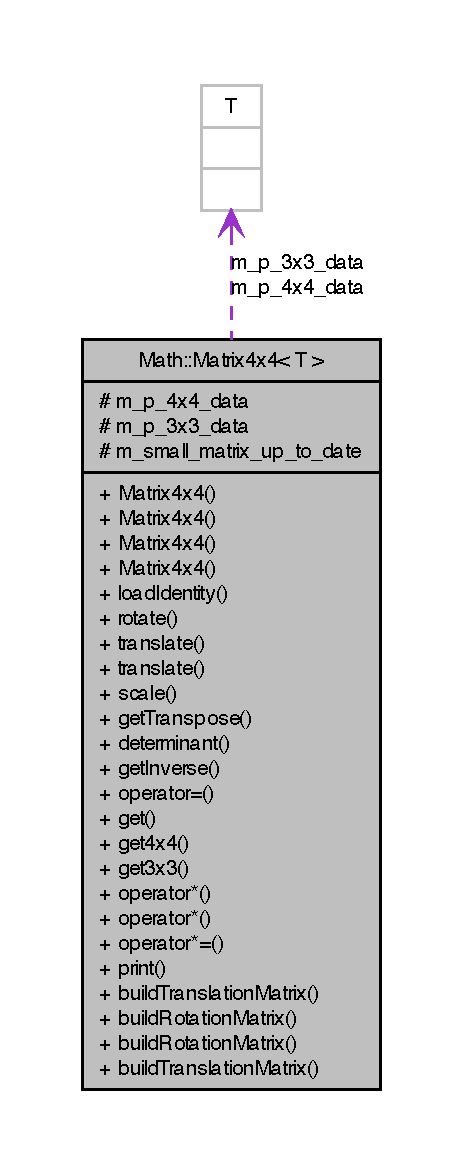
\includegraphics[width=222pt]{class_math_1_1_matrix4x4__coll__graph}
\end{center}
\end{figure}
\subsection*{Public Member Functions}
\begin{DoxyCompactItemize}
\item 
\hyperlink{class_math_1_1_matrix4x4_a583dabcedd11a91edc7dacada279e4aa}{Matrix4x4} (const T \&a1=1.0f, const T \&a2=0.0f, const T \&a3=0.0f, const T \&a4=0.0f, const T \&a5=0.0f, const T \&a6=1.0f, const T \&a7=0.0f, const T \&a8=0.0f, const T \&a9=0.0f, const T \&a10=0.0f, const T \&a11=1.0f, const T \&a12=0.0f, const T \&a13=0.0f, const T \&a14=0.0f, const T \&a15=0.0f, const T \&a16=1.0f)
\begin{DoxyCompactList}\small\item\em Default Constructor (create an identity matrix). \end{DoxyCompactList}\item 
\hyperlink{class_math_1_1_matrix4x4_ad5c78239a94616f752c798bd4f0cc65b}{Matrix4x4} (const \hyperlink{class_math_1_1_matrix4x4}{Matrix4x4} \&aMatrix)
\begin{DoxyCompactList}\small\item\em Copy Constructor. \end{DoxyCompactList}\item 
\hyperlink{class_math_1_1_matrix4x4_ab132c336e219ad10cbbdc463d78a5901}{Matrix4x4} (const \hyperlink{class_math_1_1_matrix4x4}{Matrix4x4} $\ast$apMatrix)
\begin{DoxyCompactList}\small\item\em Copy Constructor. \end{DoxyCompactList}\item 
\hyperlink{class_math_1_1_matrix4x4_a09e81e4099b8087cd9070bbda305f070}{Matrix4x4} (const T $\ast$apMatrix)
\begin{DoxyCompactList}\small\item\em Copy Constructor. \end{DoxyCompactList}\item 
void \hyperlink{class_math_1_1_matrix4x4_a3ebecfce2f332269e319462732a47f98}{loadIdentity} ()
\begin{DoxyCompactList}\small\item\em Load identity matrix. \end{DoxyCompactList}\item 
void \hyperlink{class_math_1_1_matrix4x4_a3d7bb382201ee3315ece0559453f8eac}{rotate} (const double anAngle, const \hyperlink{class_math_1_1_vec3}{Vec3}$<$ T $>$ \&aVector)
\begin{DoxyCompactList}\small\item\em Multiply the current matrix bya rotation matrix. \end{DoxyCompactList}\item 
void \hyperlink{class_math_1_1_matrix4x4_a2d75f36ee9a6ea53a8076b3cbdb7e145}{translate} (const \hyperlink{class_math_1_1_vec3}{Vec3}$<$ T $>$ \&aVector)
\begin{DoxyCompactList}\small\item\em Multiply the current matrix by a translation matrix. \end{DoxyCompactList}\item 
void \hyperlink{class_math_1_1_matrix4x4_a8b0f384bde7fc1046c981041d765f6da}{translate} (T x, T y, T z)
\begin{DoxyCompactList}\small\item\em Multiply the current matrix by a translation matrix. \end{DoxyCompactList}\item 
void \hyperlink{class_math_1_1_matrix4x4_ad1cd9ed038b29313633cc64b69e41bbd}{scale} (T x, T y, T z)
\begin{DoxyCompactList}\small\item\em Multiply the current matrix by a scaling matrix. \end{DoxyCompactList}\item 
\hyperlink{class_math_1_1_matrix4x4}{Matrix4x4} \hyperlink{class_math_1_1_matrix4x4_a123ac83bf7a9556cd7d95b9986fcca4a}{getTranspose} () const 
\begin{DoxyCompactList}\small\item\em Get the transpose of the current matrix. \end{DoxyCompactList}\item 
T \hyperlink{class_math_1_1_matrix4x4_a3fb58a8268bb16463d50e518c57e3cd7}{determinant} () const 
\begin{DoxyCompactList}\small\item\em Compute the determinant of the current matrix. \end{DoxyCompactList}\item 
\hyperlink{class_math_1_1_matrix4x4}{Matrix4x4} \hyperlink{class_math_1_1_matrix4x4_addc6d97c036220363c98220cf5fc8630}{getInverse} () const 
\begin{DoxyCompactList}\small\item\em Get the inverse of the current matrix. \end{DoxyCompactList}\item 
\hyperlink{class_math_1_1_matrix4x4}{Matrix4x4} \& \hyperlink{class_math_1_1_matrix4x4_afe3cebfecf22cb768de5fe0cbfefa1c8}{operator=} (const \hyperlink{class_math_1_1_matrix4x4}{Matrix4x4} \&aMatrix)
\begin{DoxyCompactList}\small\item\em Copy operator. \end{DoxyCompactList}\item 
const T $\ast$ \hyperlink{class_math_1_1_matrix4x4_a66f520592447586b20c6e3c6c68fbf68}{get} () const 
\begin{DoxyCompactList}\small\item\em Accessor on the 4x4 matrix data. \end{DoxyCompactList}\item 
const T $\ast$ \hyperlink{class_math_1_1_matrix4x4_a12de3ab0dc9dbe52ae41a1ff2bec1c00}{get4x4} () const 
\begin{DoxyCompactList}\small\item\em Accessor on the 4x4 matrix data. \end{DoxyCompactList}\item 
const T $\ast$ \hyperlink{class_math_1_1_matrix4x4_af06f5ea0ddf0a32e59091ee4dc95a3bd}{get3x3} ()
\begin{DoxyCompactList}\small\item\em Accessor on the 3x3 matrix data. \end{DoxyCompactList}\item 
\hyperlink{class_math_1_1_vec3}{Vec3}$<$ T $>$ \hyperlink{class_math_1_1_matrix4x4_ac5b7e2977f4c67af7a9b800aa251683f}{operator$\ast$} (const \hyperlink{class_math_1_1_vec3}{Vec3}$<$ T $>$ \&aVector) const 
\begin{DoxyCompactList}\small\item\em Operator $\ast$ to multiply the current matrix by a vector. \end{DoxyCompactList}\item 
\hyperlink{class_math_1_1_matrix4x4}{Matrix4x4} \hyperlink{class_math_1_1_matrix4x4_a0d95dc8ee2eb0a743db3f8aa9ced74a2}{operator$\ast$} (const \hyperlink{class_math_1_1_matrix4x4}{Matrix4x4} \&aMatrix) const 
\begin{DoxyCompactList}\small\item\em Operator $\ast$ to multiply the current matrix by another matrix. \end{DoxyCompactList}\item 
\hyperlink{class_math_1_1_matrix4x4}{Matrix4x4} \& \hyperlink{class_math_1_1_matrix4x4_af1f3d9263afe1d91bf2a0446f38191ba}{operator$\ast$=} (const \hyperlink{class_math_1_1_matrix4x4}{Matrix4x4} \&aMatrix)
\item 
void \hyperlink{class_math_1_1_matrix4x4_a852b4402e2c907651dd734e7a4281b2f}{print} () const 
\begin{DoxyCompactList}\small\item\em Print the matrix in the console. \end{DoxyCompactList}\end{DoxyCompactItemize}
\subsection*{Static Public Member Functions}
\begin{DoxyCompactItemize}
\item 
static \hyperlink{class_math_1_1_matrix4x4}{Matrix4x4} \hyperlink{class_math_1_1_matrix4x4_a3dc6224d52fda92a53c59338b21effaf}{buildTranslationMatrix} (const \hyperlink{class_math_1_1_vec3}{Vec3}$<$ T $>$ \&aVector)
\begin{DoxyCompactList}\small\item\em Build a tranlation matrix. \end{DoxyCompactList}\item 
static \hyperlink{class_math_1_1_matrix4x4}{Matrix4x4} \hyperlink{class_math_1_1_matrix4x4_a5dfc6ed59974a2df047d3e0008956085}{buildRotationMatrix} (T anAngle, T x, T y, T z)
\begin{DoxyCompactList}\small\item\em Build a rotation matrix. \end{DoxyCompactList}\item 
static \hyperlink{class_math_1_1_matrix4x4}{Matrix4x4} \hyperlink{class_math_1_1_matrix4x4_a0455e306c32ba2a215450b3e67ccf809}{buildRotationMatrix} (T anAngle, const \hyperlink{class_math_1_1_vec3}{Vec3}$<$ T $>$ \&aVector)
\begin{DoxyCompactList}\small\item\em Build a rotation matrix. \end{DoxyCompactList}\item 
static \hyperlink{class_math_1_1_matrix4x4}{Matrix4x4} \hyperlink{class_math_1_1_matrix4x4_a8acc0d5e8082cabad325ef9185e847e9}{buildTranslationMatrix} (T x, T y, T z)
\begin{DoxyCompactList}\small\item\em Build a rotation matrix. \end{DoxyCompactList}\end{DoxyCompactItemize}
\subsection*{Protected Attributes}
\begin{DoxyCompactItemize}
\item 
T \hyperlink{class_math_1_1_matrix4x4_a71124664bc0abb8d04c60f9d5aa3b223}{m\_\-p\_\-4x4\_\-data} \mbox{[}4 $\ast$4\mbox{]}
\begin{DoxyCompactList}\small\item\em the matrix data \end{DoxyCompactList}\item 
T \hyperlink{class_math_1_1_matrix4x4_a15e068c543d59c2035b2445f0199e267}{m\_\-p\_\-3x3\_\-data} \mbox{[}3 $\ast$3\mbox{]}
\begin{DoxyCompactList}\small\item\em the matrix data \end{DoxyCompactList}\item 
bool \hyperlink{class_math_1_1_matrix4x4_ab2beab6050bc7e8a170b7f2121aeefb5}{m\_\-small\_\-matrix\_\-up\_\-to\_\-date}
\end{DoxyCompactItemize}


\subsection{Detailed Description}
\subsubsection*{template$<$typename T$>$class Math::Matrix4x4$<$ T $>$}

\hyperlink{class_math_1_1_matrix4x4}{Matrix4x4} is a template class to handle a 4 by 4 matrix. 

Definition at line 53 of file Matrix4x4.h.



\subsection{Constructor \& Destructor Documentation}
\hypertarget{class_math_1_1_matrix4x4_a583dabcedd11a91edc7dacada279e4aa}{
\index{Math::Matrix4x4@{Math::Matrix4x4}!Matrix4x4@{Matrix4x4}}
\index{Matrix4x4@{Matrix4x4}!Math::Matrix4x4@{Math::Matrix4x4}}
\subsubsection[{Matrix4x4}]{\setlength{\rightskip}{0pt plus 5cm}template$<$typename T$>$ {\bf Math::Matrix4x4}$<$ T $>$::{\bf Matrix4x4} (
\begin{DoxyParamCaption}
\item[{const T \&}]{a1 = {\ttfamily 1.0f}, }
\item[{const T \&}]{a2 = {\ttfamily 0.0f}, }
\item[{const T \&}]{a3 = {\ttfamily 0.0f}, }
\item[{const T \&}]{a4 = {\ttfamily 0.0f}, }
\item[{const T \&}]{a5 = {\ttfamily 0.0f}, }
\item[{const T \&}]{a6 = {\ttfamily 1.0f}, }
\item[{const T \&}]{a7 = {\ttfamily 0.0f}, }
\item[{const T \&}]{a8 = {\ttfamily 0.0f}, }
\item[{const T \&}]{a9 = {\ttfamily 0.0f}, }
\item[{const T \&}]{a10 = {\ttfamily 0.0f}, }
\item[{const T \&}]{a11 = {\ttfamily 1.0f}, }
\item[{const T \&}]{a12 = {\ttfamily 0.0f}, }
\item[{const T \&}]{a13 = {\ttfamily 0.0f}, }
\item[{const T \&}]{a14 = {\ttfamily 0.0f}, }
\item[{const T \&}]{a15 = {\ttfamily 0.0f}, }
\item[{const T \&}]{a16 = {\ttfamily 1.0f}}
\end{DoxyParamCaption}
)}}
\label{class_math_1_1_matrix4x4_a583dabcedd11a91edc7dacada279e4aa}


Default Constructor (create an identity matrix). 


\begin{DoxyParams}{Parameters}
{\em a1,:} & the 1st element of the matrix \\
\hline
{\em a2,:} & the 2nd element of the matrix \\
\hline
{\em a3,:} & the 3rd element of the matrix \\
\hline
{\em a4,:} & the 4th element of the matrix \\
\hline
{\em a5,:} & the 5th element of the matrix \\
\hline
{\em a6,:} & the 6th element of the matrix \\
\hline
{\em a7,:} & the 7th element of the matrix \\
\hline
{\em a8,:} & the 8th element of the matrix \\
\hline
{\em a9,:} & the 9th element of the matrix \\
\hline
{\em a10,:} & the 10th element of the matrix \\
\hline
{\em a11,:} & the 11th element of the matrix \\
\hline
{\em a12,:} & the 12th element of the matrix \\
\hline
{\em a13,:} & the 13th element of the matrix \\
\hline
{\em a14,:} & the 14th element of the matrix \\
\hline
{\em a15,:} & the 15th element of the matrix \\
\hline
{\em a16,:} & the 16th element of the matrix \\
\hline
\end{DoxyParams}


Definition at line 48 of file Matrix4x4.inl.

\hypertarget{class_math_1_1_matrix4x4_ad5c78239a94616f752c798bd4f0cc65b}{
\index{Math::Matrix4x4@{Math::Matrix4x4}!Matrix4x4@{Matrix4x4}}
\index{Matrix4x4@{Matrix4x4}!Math::Matrix4x4@{Math::Matrix4x4}}
\subsubsection[{Matrix4x4}]{\setlength{\rightskip}{0pt plus 5cm}template$<$typename T$>$ {\bf Math::Matrix4x4}$<$ T $>$::{\bf Matrix4x4} (
\begin{DoxyParamCaption}
\item[{const {\bf Matrix4x4}$<$ T $>$ \&}]{aMatrix}
\end{DoxyParamCaption}
)}}
\label{class_math_1_1_matrix4x4_ad5c78239a94616f752c798bd4f0cc65b}


Copy Constructor. 


\begin{DoxyParams}{Parameters}
{\em aMatrix,:} & the matrix to copy \\
\hline
\end{DoxyParams}


Definition at line 76 of file Matrix4x4.inl.

\hypertarget{class_math_1_1_matrix4x4_ab132c336e219ad10cbbdc463d78a5901}{
\index{Math::Matrix4x4@{Math::Matrix4x4}!Matrix4x4@{Matrix4x4}}
\index{Matrix4x4@{Matrix4x4}!Math::Matrix4x4@{Math::Matrix4x4}}
\subsubsection[{Matrix4x4}]{\setlength{\rightskip}{0pt plus 5cm}template$<$typename T$>$ {\bf Math::Matrix4x4}$<$ T $>$::{\bf Matrix4x4} (
\begin{DoxyParamCaption}
\item[{const {\bf Matrix4x4}$<$ T $>$ $\ast$}]{apMatrix}
\end{DoxyParamCaption}
)}}
\label{class_math_1_1_matrix4x4_ab132c336e219ad10cbbdc463d78a5901}


Copy Constructor. 


\begin{DoxyParams}{Parameters}
{\em apMatrix,:} & the matrix to copy \\
\hline
\end{DoxyParams}
\hypertarget{class_math_1_1_matrix4x4_a09e81e4099b8087cd9070bbda305f070}{
\index{Math::Matrix4x4@{Math::Matrix4x4}!Matrix4x4@{Matrix4x4}}
\index{Matrix4x4@{Matrix4x4}!Math::Matrix4x4@{Math::Matrix4x4}}
\subsubsection[{Matrix4x4}]{\setlength{\rightskip}{0pt plus 5cm}template$<$typename T$>$ {\bf Math::Matrix4x4}$<$ T $>$::{\bf Matrix4x4} (
\begin{DoxyParamCaption}
\item[{const T $\ast$}]{apMatrix}
\end{DoxyParamCaption}
)}}
\label{class_math_1_1_matrix4x4_a09e81e4099b8087cd9070bbda305f070}


Copy Constructor. 


\begin{DoxyParams}{Parameters}
{\em apMatrix,:} & the matrix to copy \\
\hline
\end{DoxyParams}


Definition at line 86 of file Matrix4x4.inl.



\subsection{Member Function Documentation}
\hypertarget{class_math_1_1_matrix4x4_a5dfc6ed59974a2df047d3e0008956085}{
\index{Math::Matrix4x4@{Math::Matrix4x4}!buildRotationMatrix@{buildRotationMatrix}}
\index{buildRotationMatrix@{buildRotationMatrix}!Math::Matrix4x4@{Math::Matrix4x4}}
\subsubsection[{buildRotationMatrix}]{\setlength{\rightskip}{0pt plus 5cm}template$<$typename T$>$ {\bf Matrix4x4}$<$ T $>$ {\bf Math::Matrix4x4}$<$ T $>$::buildRotationMatrix (
\begin{DoxyParamCaption}
\item[{T}]{anAngle, }
\item[{T}]{x, }
\item[{T}]{y, }
\item[{T}]{z}
\end{DoxyParamCaption}
)\hspace{0.3cm}{\ttfamily  \mbox{[}static\mbox{]}}}}
\label{class_math_1_1_matrix4x4_a5dfc6ed59974a2df047d3e0008956085}


Build a rotation matrix. 


\begin{DoxyParams}{Parameters}
{\em anAngle,:} & the angle of rotation in degrees \\
\hline
{\em x,:} & the x-\/component of the axis of rotation \\
\hline
{\em y,:} & the y-\/component of the axis of rotation \\
\hline
{\em z,:} & the z-\/component of the axis of rotation \\
\hline
\end{DoxyParams}
\begin{DoxyReturn}{Returns}
the corresponding rotation matrix 
\end{DoxyReturn}


Definition at line 183 of file Matrix4x4.inl.

\hypertarget{class_math_1_1_matrix4x4_a0455e306c32ba2a215450b3e67ccf809}{
\index{Math::Matrix4x4@{Math::Matrix4x4}!buildRotationMatrix@{buildRotationMatrix}}
\index{buildRotationMatrix@{buildRotationMatrix}!Math::Matrix4x4@{Math::Matrix4x4}}
\subsubsection[{buildRotationMatrix}]{\setlength{\rightskip}{0pt plus 5cm}template$<$typename T$>$ {\bf Matrix4x4}$<$ T $>$ {\bf Math::Matrix4x4}$<$ T $>$::buildRotationMatrix (
\begin{DoxyParamCaption}
\item[{T}]{anAngle, }
\item[{const {\bf Vec3}$<$ T $>$ \&}]{aVector}
\end{DoxyParamCaption}
)\hspace{0.3cm}{\ttfamily  \mbox{[}static\mbox{]}}}}
\label{class_math_1_1_matrix4x4_a0455e306c32ba2a215450b3e67ccf809}


Build a rotation matrix. 


\begin{DoxyParams}{Parameters}
{\em anAngle,:} & the angle of rotation in degrees \\
\hline
{\em aVector,:} & the axis of rotation \\
\hline
\end{DoxyParams}
\begin{DoxyReturn}{Returns}
the corresponding translation matrix 
\end{DoxyReturn}


Definition at line 174 of file Matrix4x4.inl.

\hypertarget{class_math_1_1_matrix4x4_a8acc0d5e8082cabad325ef9185e847e9}{
\index{Math::Matrix4x4@{Math::Matrix4x4}!buildTranslationMatrix@{buildTranslationMatrix}}
\index{buildTranslationMatrix@{buildTranslationMatrix}!Math::Matrix4x4@{Math::Matrix4x4}}
\subsubsection[{buildTranslationMatrix}]{\setlength{\rightskip}{0pt plus 5cm}template$<$typename T$>$ {\bf Matrix4x4}$<$ T $>$ {\bf Math::Matrix4x4}$<$ T $>$::buildTranslationMatrix (
\begin{DoxyParamCaption}
\item[{T}]{x, }
\item[{T}]{y, }
\item[{T}]{z}
\end{DoxyParamCaption}
)\hspace{0.3cm}{\ttfamily  \mbox{[}static\mbox{]}}}}
\label{class_math_1_1_matrix4x4_a8acc0d5e8082cabad325ef9185e847e9}


Build a rotation matrix. 


\begin{DoxyParams}{Parameters}
{\em x,:} & the x-\/component of the translation vector \\
\hline
{\em y,:} & the y-\/component of the translation vector \\
\hline
{\em z,:} & the z-\/component of the translation vector \\
\hline
\end{DoxyParams}
\begin{DoxyReturn}{Returns}
the corresponding translation matrix 
\end{DoxyReturn}


Definition at line 162 of file Matrix4x4.inl.

\hypertarget{class_math_1_1_matrix4x4_a3dc6224d52fda92a53c59338b21effaf}{
\index{Math::Matrix4x4@{Math::Matrix4x4}!buildTranslationMatrix@{buildTranslationMatrix}}
\index{buildTranslationMatrix@{buildTranslationMatrix}!Math::Matrix4x4@{Math::Matrix4x4}}
\subsubsection[{buildTranslationMatrix}]{\setlength{\rightskip}{0pt plus 5cm}template$<$typename T$>$ {\bf Matrix4x4}$<$ T $>$ {\bf Math::Matrix4x4}$<$ T $>$::buildTranslationMatrix (
\begin{DoxyParamCaption}
\item[{const {\bf Vec3}$<$ T $>$ \&}]{aVector}
\end{DoxyParamCaption}
)\hspace{0.3cm}{\ttfamily  \mbox{[}static\mbox{]}}}}
\label{class_math_1_1_matrix4x4_a3dc6224d52fda92a53c59338b21effaf}


Build a tranlation matrix. 


\begin{DoxyParams}{Parameters}
{\em aVector,:} & the translation vector \\
\hline
\end{DoxyParams}
\begin{DoxyReturn}{Returns}
the corresponding translation matrix 
\end{DoxyReturn}


Definition at line 154 of file Matrix4x4.inl.

\hypertarget{class_math_1_1_matrix4x4_a3fb58a8268bb16463d50e518c57e3cd7}{
\index{Math::Matrix4x4@{Math::Matrix4x4}!determinant@{determinant}}
\index{determinant@{determinant}!Math::Matrix4x4@{Math::Matrix4x4}}
\subsubsection[{determinant}]{\setlength{\rightskip}{0pt plus 5cm}template$<$typename T $>$ T {\bf Math::Matrix4x4}$<$ T $>$::determinant (
\begin{DoxyParamCaption}
{}
\end{DoxyParamCaption}
) const}}
\label{class_math_1_1_matrix4x4_a3fb58a8268bb16463d50e518c57e3cd7}


Compute the determinant of the current matrix. 

\begin{DoxyReturn}{Returns}
the determinant 
\end{DoxyReturn}


Definition at line 250 of file Matrix4x4.inl.

\hypertarget{class_math_1_1_matrix4x4_a66f520592447586b20c6e3c6c68fbf68}{
\index{Math::Matrix4x4@{Math::Matrix4x4}!get@{get}}
\index{get@{get}!Math::Matrix4x4@{Math::Matrix4x4}}
\subsubsection[{get}]{\setlength{\rightskip}{0pt plus 5cm}template$<$typename T $>$ const T $\ast$ {\bf Math::Matrix4x4}$<$ T $>$::get (
\begin{DoxyParamCaption}
{}
\end{DoxyParamCaption}
) const}}
\label{class_math_1_1_matrix4x4_a66f520592447586b20c6e3c6c68fbf68}


Accessor on the 4x4 matrix data. 

\begin{DoxyReturn}{Returns}
the matrix raw data 
\end{DoxyReturn}


Definition at line 362 of file Matrix4x4.inl.

\hypertarget{class_math_1_1_matrix4x4_af06f5ea0ddf0a32e59091ee4dc95a3bd}{
\index{Math::Matrix4x4@{Math::Matrix4x4}!get3x3@{get3x3}}
\index{get3x3@{get3x3}!Math::Matrix4x4@{Math::Matrix4x4}}
\subsubsection[{get3x3}]{\setlength{\rightskip}{0pt plus 5cm}template$<$typename T $>$ const T $\ast$ {\bf Math::Matrix4x4}$<$ T $>$::get3x3 (
\begin{DoxyParamCaption}
{}
\end{DoxyParamCaption}
)}}
\label{class_math_1_1_matrix4x4_af06f5ea0ddf0a32e59091ee4dc95a3bd}


Accessor on the 3x3 matrix data. 

\begin{DoxyReturn}{Returns}
the matrix raw data 
\end{DoxyReturn}


Definition at line 378 of file Matrix4x4.inl.

\hypertarget{class_math_1_1_matrix4x4_a12de3ab0dc9dbe52ae41a1ff2bec1c00}{
\index{Math::Matrix4x4@{Math::Matrix4x4}!get4x4@{get4x4}}
\index{get4x4@{get4x4}!Math::Matrix4x4@{Math::Matrix4x4}}
\subsubsection[{get4x4}]{\setlength{\rightskip}{0pt plus 5cm}template$<$typename T $>$ const T $\ast$ {\bf Math::Matrix4x4}$<$ T $>$::get4x4 (
\begin{DoxyParamCaption}
{}
\end{DoxyParamCaption}
) const}}
\label{class_math_1_1_matrix4x4_a12de3ab0dc9dbe52ae41a1ff2bec1c00}


Accessor on the 4x4 matrix data. 

\begin{DoxyReturn}{Returns}
the matrix raw data 
\end{DoxyReturn}


Definition at line 370 of file Matrix4x4.inl.

\hypertarget{class_math_1_1_matrix4x4_addc6d97c036220363c98220cf5fc8630}{
\index{Math::Matrix4x4@{Math::Matrix4x4}!getInverse@{getInverse}}
\index{getInverse@{getInverse}!Math::Matrix4x4@{Math::Matrix4x4}}
\subsubsection[{getInverse}]{\setlength{\rightskip}{0pt plus 5cm}template$<$typename T $>$ {\bf Matrix4x4}$<$ T $>$ {\bf Math::Matrix4x4}$<$ T $>$::getInverse (
\begin{DoxyParamCaption}
{}
\end{DoxyParamCaption}
) const}}
\label{class_math_1_1_matrix4x4_addc6d97c036220363c98220cf5fc8630}


Get the inverse of the current matrix. 

\begin{DoxyReturn}{Returns}
the inverse matrix 
\end{DoxyReturn}


Definition at line 264 of file Matrix4x4.inl.

\hypertarget{class_math_1_1_matrix4x4_a123ac83bf7a9556cd7d95b9986fcca4a}{
\index{Math::Matrix4x4@{Math::Matrix4x4}!getTranspose@{getTranspose}}
\index{getTranspose@{getTranspose}!Math::Matrix4x4@{Math::Matrix4x4}}
\subsubsection[{getTranspose}]{\setlength{\rightskip}{0pt plus 5cm}template$<$typename T $>$ {\bf Matrix4x4}$<$ T $>$ {\bf Math::Matrix4x4}$<$ T $>$::getTranspose (
\begin{DoxyParamCaption}
{}
\end{DoxyParamCaption}
) const}}
\label{class_math_1_1_matrix4x4_a123ac83bf7a9556cd7d95b9986fcca4a}


Get the transpose of the current matrix. 

\begin{DoxyReturn}{Returns}
the transpose matrix 
\end{DoxyReturn}


Definition at line 238 of file Matrix4x4.inl.

\hypertarget{class_math_1_1_matrix4x4_a3ebecfce2f332269e319462732a47f98}{
\index{Math::Matrix4x4@{Math::Matrix4x4}!loadIdentity@{loadIdentity}}
\index{loadIdentity@{loadIdentity}!Math::Matrix4x4@{Math::Matrix4x4}}
\subsubsection[{loadIdentity}]{\setlength{\rightskip}{0pt plus 5cm}template$<$typename T $>$ void {\bf Math::Matrix4x4}$<$ T $>$::loadIdentity (
\begin{DoxyParamCaption}
{}
\end{DoxyParamCaption}
)}}
\label{class_math_1_1_matrix4x4_a3ebecfce2f332269e319462732a47f98}


Load identity matrix. 



Definition at line 96 of file Matrix4x4.inl.

\hypertarget{class_math_1_1_matrix4x4_ac5b7e2977f4c67af7a9b800aa251683f}{
\index{Math::Matrix4x4@{Math::Matrix4x4}!operator$\ast$@{operator$\ast$}}
\index{operator$\ast$@{operator$\ast$}!Math::Matrix4x4@{Math::Matrix4x4}}
\subsubsection[{operator$\ast$}]{\setlength{\rightskip}{0pt plus 5cm}template$<$typename T$>$ {\bf Vec3}$<$ T $>$ {\bf Math::Matrix4x4}$<$ T $>$::operator$\ast$ (
\begin{DoxyParamCaption}
\item[{const {\bf Vec3}$<$ T $>$ \&}]{aVector}
\end{DoxyParamCaption}
) const}}
\label{class_math_1_1_matrix4x4_ac5b7e2977f4c67af7a9b800aa251683f}


Operator $\ast$ to multiply the current matrix by a vector. 


\begin{DoxyParams}{Parameters}
{\em aVector,:} & the vector to transform \\
\hline
\end{DoxyParams}
\begin{DoxyReturn}{Returns}
the transformed vector 
\end{DoxyReturn}


Definition at line 307 of file Matrix4x4.inl.

\hypertarget{class_math_1_1_matrix4x4_a0d95dc8ee2eb0a743db3f8aa9ced74a2}{
\index{Math::Matrix4x4@{Math::Matrix4x4}!operator$\ast$@{operator$\ast$}}
\index{operator$\ast$@{operator$\ast$}!Math::Matrix4x4@{Math::Matrix4x4}}
\subsubsection[{operator$\ast$}]{\setlength{\rightskip}{0pt plus 5cm}template$<$typename T$>$ {\bf Matrix4x4}$<$ T $>$ {\bf Math::Matrix4x4}$<$ T $>$::operator$\ast$ (
\begin{DoxyParamCaption}
\item[{const {\bf Matrix4x4}$<$ T $>$ \&}]{aMatrix}
\end{DoxyParamCaption}
) const}}
\label{class_math_1_1_matrix4x4_a0d95dc8ee2eb0a743db3f8aa9ced74a2}


Operator $\ast$ to multiply the current matrix by another matrix. 


\begin{DoxyParams}{Parameters}
{\em aMatrix,:} & the other matrix \\
\hline
\end{DoxyParams}
\begin{DoxyReturn}{Returns}
the transformed matrix 
\end{DoxyReturn}


Definition at line 320 of file Matrix4x4.inl.

\hypertarget{class_math_1_1_matrix4x4_af1f3d9263afe1d91bf2a0446f38191ba}{
\index{Math::Matrix4x4@{Math::Matrix4x4}!operator$\ast$=@{operator$\ast$=}}
\index{operator$\ast$=@{operator$\ast$=}!Math::Matrix4x4@{Math::Matrix4x4}}
\subsubsection[{operator$\ast$=}]{\setlength{\rightskip}{0pt plus 5cm}template$<$typename T $>$ {\bf Matrix4x4}$<$ T $>$ \& {\bf Math::Matrix4x4}$<$ T $>$::operator$\ast$= (
\begin{DoxyParamCaption}
\item[{const {\bf Matrix4x4}$<$ T $>$ \&}]{aMatrix}
\end{DoxyParamCaption}
)}}
\label{class_math_1_1_matrix4x4_af1f3d9263afe1d91bf2a0446f38191ba}
Operator $\ast$= to multiply the current matrix by another matrix, and modify the current matrix. 
\begin{DoxyParams}{Parameters}
{\em aMatrix,:} & the other matrix \\
\hline
\end{DoxyParams}
\begin{DoxyReturn}{Returns}
the transformed matrix 
\end{DoxyReturn}


Definition at line 350 of file Matrix4x4.inl.

\hypertarget{class_math_1_1_matrix4x4_afe3cebfecf22cb768de5fe0cbfefa1c8}{
\index{Math::Matrix4x4@{Math::Matrix4x4}!operator=@{operator=}}
\index{operator=@{operator=}!Math::Matrix4x4@{Math::Matrix4x4}}
\subsubsection[{operator=}]{\setlength{\rightskip}{0pt plus 5cm}template$<$typename T $>$ {\bf Matrix4x4}$<$ T $>$ \& {\bf Math::Matrix4x4}$<$ T $>$::operator= (
\begin{DoxyParamCaption}
\item[{const {\bf Matrix4x4}$<$ T $>$ \&}]{aMatrix}
\end{DoxyParamCaption}
)}}
\label{class_math_1_1_matrix4x4_afe3cebfecf22cb768de5fe0cbfefa1c8}


Copy operator. 


\begin{DoxyParams}{Parameters}
{\em aMatrix,:} & the matrix to copy \\
\hline
\end{DoxyParams}
\begin{DoxyReturn}{Returns}
the copied matrix 
\end{DoxyReturn}


Definition at line 295 of file Matrix4x4.inl.

\hypertarget{class_math_1_1_matrix4x4_a852b4402e2c907651dd734e7a4281b2f}{
\index{Math::Matrix4x4@{Math::Matrix4x4}!print@{print}}
\index{print@{print}!Math::Matrix4x4@{Math::Matrix4x4}}
\subsubsection[{print}]{\setlength{\rightskip}{0pt plus 5cm}template$<$typename T $>$ void {\bf Math::Matrix4x4}$<$ T $>$::print (
\begin{DoxyParamCaption}
{}
\end{DoxyParamCaption}
) const}}
\label{class_math_1_1_matrix4x4_a852b4402e2c907651dd734e7a4281b2f}


Print the matrix in the console. 



Definition at line 404 of file Matrix4x4.inl.

\hypertarget{class_math_1_1_matrix4x4_a3d7bb382201ee3315ece0559453f8eac}{
\index{Math::Matrix4x4@{Math::Matrix4x4}!rotate@{rotate}}
\index{rotate@{rotate}!Math::Matrix4x4@{Math::Matrix4x4}}
\subsubsection[{rotate}]{\setlength{\rightskip}{0pt plus 5cm}template$<$typename T$>$ void {\bf Math::Matrix4x4}$<$ T $>$::rotate (
\begin{DoxyParamCaption}
\item[{const double}]{anAngle, }
\item[{const {\bf Vec3}$<$ T $>$ \&}]{aVector}
\end{DoxyParamCaption}
)}}
\label{class_math_1_1_matrix4x4_a3d7bb382201ee3315ece0559453f8eac}


Multiply the current matrix bya rotation matrix. 


\begin{DoxyParams}{Parameters}
{\em anAngle,:} & the angle of rotation in degrees \\
\hline
{\em aVector,:} & the axis of rotation \\
\hline
\end{DoxyParams}


Definition at line 124 of file Matrix4x4.inl.

\hypertarget{class_math_1_1_matrix4x4_ad1cd9ed038b29313633cc64b69e41bbd}{
\index{Math::Matrix4x4@{Math::Matrix4x4}!scale@{scale}}
\index{scale@{scale}!Math::Matrix4x4@{Math::Matrix4x4}}
\subsubsection[{scale}]{\setlength{\rightskip}{0pt plus 5cm}template$<$typename T$>$ void {\bf Math::Matrix4x4}$<$ T $>$::scale (
\begin{DoxyParamCaption}
\item[{T}]{x, }
\item[{T}]{y, }
\item[{T}]{z}
\end{DoxyParamCaption}
)}}
\label{class_math_1_1_matrix4x4_ad1cd9ed038b29313633cc64b69e41bbd}


Multiply the current matrix by a scaling matrix. 


\begin{DoxyParams}{Parameters}
{\em x,:} & the scaling factor along the X-\/axis \\
\hline
{\em y,:} & the scaling factor along the Y-\/axis \\
\hline
{\em z,:} & the scaling factor along the Z-\/axis \\
\hline
\end{DoxyParams}


Definition at line 222 of file Matrix4x4.inl.

\hypertarget{class_math_1_1_matrix4x4_a8b0f384bde7fc1046c981041d765f6da}{
\index{Math::Matrix4x4@{Math::Matrix4x4}!translate@{translate}}
\index{translate@{translate}!Math::Matrix4x4@{Math::Matrix4x4}}
\subsubsection[{translate}]{\setlength{\rightskip}{0pt plus 5cm}template$<$typename T$>$ void {\bf Math::Matrix4x4}$<$ T $>$::translate (
\begin{DoxyParamCaption}
\item[{T}]{x, }
\item[{T}]{y, }
\item[{T}]{z}
\end{DoxyParamCaption}
)}}
\label{class_math_1_1_matrix4x4_a8b0f384bde7fc1046c981041d765f6da}


Multiply the current matrix by a translation matrix. 


\begin{DoxyParams}{Parameters}
{\em x,:} & the x-\/component of the translation vector \\
\hline
{\em y,:} & the y-\/component of the translation vector \\
\hline
{\em z,:} & the z-\/component of the translation vector \\
\hline
\end{DoxyParams}


Definition at line 144 of file Matrix4x4.inl.

\hypertarget{class_math_1_1_matrix4x4_a2d75f36ee9a6ea53a8076b3cbdb7e145}{
\index{Math::Matrix4x4@{Math::Matrix4x4}!translate@{translate}}
\index{translate@{translate}!Math::Matrix4x4@{Math::Matrix4x4}}
\subsubsection[{translate}]{\setlength{\rightskip}{0pt plus 5cm}template$<$typename T$>$ void {\bf Math::Matrix4x4}$<$ T $>$::translate (
\begin{DoxyParamCaption}
\item[{const {\bf Vec3}$<$ T $>$ \&}]{aVector}
\end{DoxyParamCaption}
)}}
\label{class_math_1_1_matrix4x4_a2d75f36ee9a6ea53a8076b3cbdb7e145}


Multiply the current matrix by a translation matrix. 


\begin{DoxyParams}{Parameters}
{\em aVector,:} & the translation vector \\
\hline
\end{DoxyParams}


Definition at line 134 of file Matrix4x4.inl.



\subsection{Member Data Documentation}
\hypertarget{class_math_1_1_matrix4x4_a15e068c543d59c2035b2445f0199e267}{
\index{Math::Matrix4x4@{Math::Matrix4x4}!m\_\-p\_\-3x3\_\-data@{m\_\-p\_\-3x3\_\-data}}
\index{m\_\-p\_\-3x3\_\-data@{m\_\-p\_\-3x3\_\-data}!Math::Matrix4x4@{Math::Matrix4x4}}
\subsubsection[{m\_\-p\_\-3x3\_\-data}]{\setlength{\rightskip}{0pt plus 5cm}template$<$typename T$>$ T {\bf Math::Matrix4x4}$<$ T $>$::{\bf m\_\-p\_\-3x3\_\-data}\mbox{[}3 $\ast$3\mbox{]}\hspace{0.3cm}{\ttfamily  \mbox{[}protected\mbox{]}}}}
\label{class_math_1_1_matrix4x4_a15e068c543d59c2035b2445f0199e267}


the matrix data 



Definition at line 313 of file Matrix4x4.h.

\hypertarget{class_math_1_1_matrix4x4_a71124664bc0abb8d04c60f9d5aa3b223}{
\index{Math::Matrix4x4@{Math::Matrix4x4}!m\_\-p\_\-4x4\_\-data@{m\_\-p\_\-4x4\_\-data}}
\index{m\_\-p\_\-4x4\_\-data@{m\_\-p\_\-4x4\_\-data}!Math::Matrix4x4@{Math::Matrix4x4}}
\subsubsection[{m\_\-p\_\-4x4\_\-data}]{\setlength{\rightskip}{0pt plus 5cm}template$<$typename T$>$ T {\bf Math::Matrix4x4}$<$ T $>$::{\bf m\_\-p\_\-4x4\_\-data}\mbox{[}4 $\ast$4\mbox{]}\hspace{0.3cm}{\ttfamily  \mbox{[}protected\mbox{]}}}}
\label{class_math_1_1_matrix4x4_a71124664bc0abb8d04c60f9d5aa3b223}


the matrix data 



Definition at line 309 of file Matrix4x4.h.

\hypertarget{class_math_1_1_matrix4x4_ab2beab6050bc7e8a170b7f2121aeefb5}{
\index{Math::Matrix4x4@{Math::Matrix4x4}!m\_\-small\_\-matrix\_\-up\_\-to\_\-date@{m\_\-small\_\-matrix\_\-up\_\-to\_\-date}}
\index{m\_\-small\_\-matrix\_\-up\_\-to\_\-date@{m\_\-small\_\-matrix\_\-up\_\-to\_\-date}!Math::Matrix4x4@{Math::Matrix4x4}}
\subsubsection[{m\_\-small\_\-matrix\_\-up\_\-to\_\-date}]{\setlength{\rightskip}{0pt plus 5cm}template$<$typename T$>$ bool {\bf Math::Matrix4x4}$<$ T $>$::{\bf m\_\-small\_\-matrix\_\-up\_\-to\_\-date}\hspace{0.3cm}{\ttfamily  \mbox{[}protected\mbox{]}}}}
\label{class_math_1_1_matrix4x4_ab2beab6050bc7e8a170b7f2121aeefb5}
A flag to check if the 3x3 matrix is up-\/to-\/date. It is used for lazy evaluation. 

Definition at line 318 of file Matrix4x4.h.



The documentation for this class was generated from the following files:\begin{DoxyCompactItemize}
\item 
/Users/fpvidal/Documents/gvirtualxray-\/code/trunk/include/gVirtualXRay/\hyperlink{_matrix4x4_8h}{Matrix4x4.h}\item 
/Users/fpvidal/Documents/gvirtualxray-\/code/trunk/include/gVirtualXRay/\hyperlink{_matrix4x4_8inl}{Matrix4x4.inl}\end{DoxyCompactItemize}

\hypertarget{class_utilities_1_1_open_g_l_exception}{
\section{Utilities::OpenGLException Class Reference}
\label{class_utilities_1_1_open_g_l_exception}\index{Utilities::OpenGLException@{Utilities::OpenGLException}}
}


\hyperlink{class_utilities_1_1_open_g_l_exception}{OpenGLException} is a class to handle exceptions related to OpenGL.  




{\ttfamily \#include $<$OpenGLException.h$>$}



Inheritance diagram for Utilities::OpenGLException:\nopagebreak
\begin{figure}[H]
\begin{center}
\leavevmode
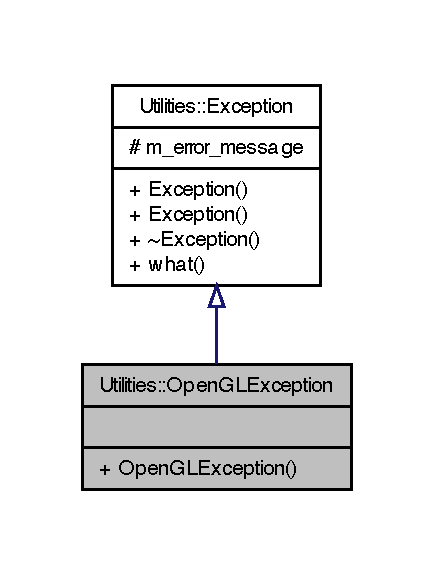
\includegraphics[width=208pt]{class_utilities_1_1_open_g_l_exception__inherit__graph}
\end{center}
\end{figure}


Collaboration diagram for Utilities::OpenGLException:\nopagebreak
\begin{figure}[H]
\begin{center}
\leavevmode
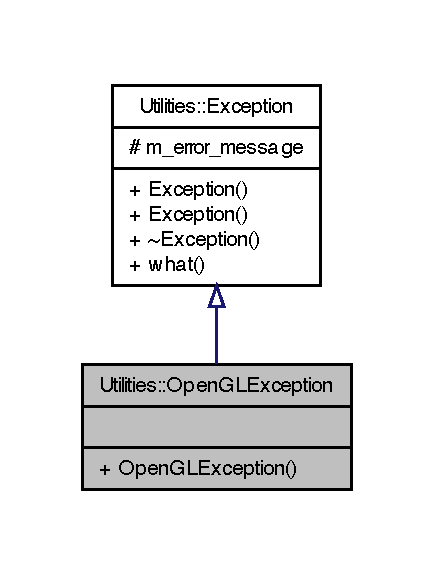
\includegraphics[width=208pt]{class_utilities_1_1_open_g_l_exception__coll__graph}
\end{center}
\end{figure}
\subsection*{Public Member Functions}
\begin{DoxyCompactItemize}
\item 
\hyperlink{class_utilities_1_1_open_g_l_exception_a43403a6b915c82a7325bd927e1a2274d}{OpenGLException} (const char $\ast$aFileName, const char $\ast$aFunctionName, int anErrorLine, int anErrorCode)
\begin{DoxyCompactList}\small\item\em Default constructor. \end{DoxyCompactList}\end{DoxyCompactItemize}


\subsection{Detailed Description}
\hyperlink{class_utilities_1_1_open_g_l_exception}{OpenGLException} is a class to handle exceptions related to OpenGL. 

Definition at line 53 of file OpenGLException.h.



\subsection{Constructor \& Destructor Documentation}
\hypertarget{class_utilities_1_1_open_g_l_exception_a43403a6b915c82a7325bd927e1a2274d}{
\index{Utilities::OpenGLException@{Utilities::OpenGLException}!OpenGLException@{OpenGLException}}
\index{OpenGLException@{OpenGLException}!Utilities::OpenGLException@{Utilities::OpenGLException}}
\subsubsection[{OpenGLException}]{\setlength{\rightskip}{0pt plus 5cm}Utilities::OpenGLException::OpenGLException (
\begin{DoxyParamCaption}
\item[{const char $\ast$}]{aFileName, }
\item[{const char $\ast$}]{aFunctionName, }
\item[{int}]{anErrorLine, }
\item[{int}]{anErrorCode}
\end{DoxyParamCaption}
)}}
\label{class_utilities_1_1_open_g_l_exception_a43403a6b915c82a7325bd927e1a2274d}


Default constructor. 


\begin{DoxyParams}{Parameters}
{\em aFileName,:} & name of the source file where the exception was thrown \\
\hline
{\em aFunctionName,:} & name of the function where the exception was thrown \\
\hline
{\em anErrorLine,:} & name at which the exception was thrown \\
\hline
{\em anErrorCode,:} & OpenGL error code \\
\hline
\end{DoxyParams}


The documentation for this class was generated from the following file:\begin{DoxyCompactItemize}
\item 
/Users/fpvidal/Documents/gvirtualxray-\/code/trunk/include/gVirtualXRay/\hyperlink{_open_g_l_exception_8h}{OpenGLException.h}\end{DoxyCompactItemize}

\hypertarget{class_utilities_1_1_out_of_bounds_exception}{
\section{Utilities::OutOfBoundsException Class Reference}
\label{class_utilities_1_1_out_of_bounds_exception}\index{Utilities::OutOfBoundsException@{Utilities::OutOfBoundsException}}
}


{\ttfamily \#include $<$OutOfBoundsException.h$>$}



Inheritance diagram for Utilities::OutOfBoundsException:\nopagebreak
\begin{figure}[H]
\begin{center}
\leavevmode
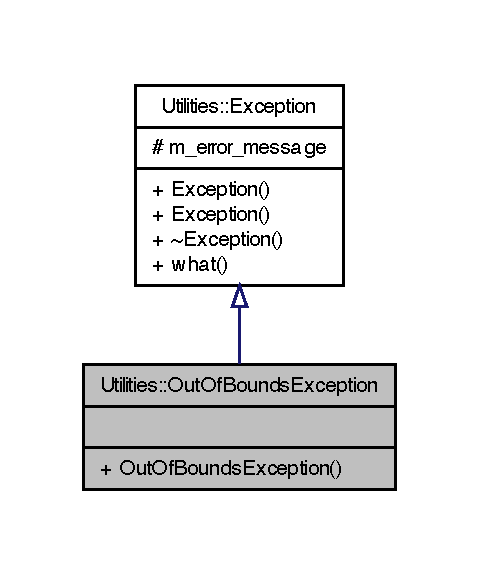
\includegraphics[width=230pt]{class_utilities_1_1_out_of_bounds_exception__inherit__graph}
\end{center}
\end{figure}


Collaboration diagram for Utilities::OutOfBoundsException:\nopagebreak
\begin{figure}[H]
\begin{center}
\leavevmode
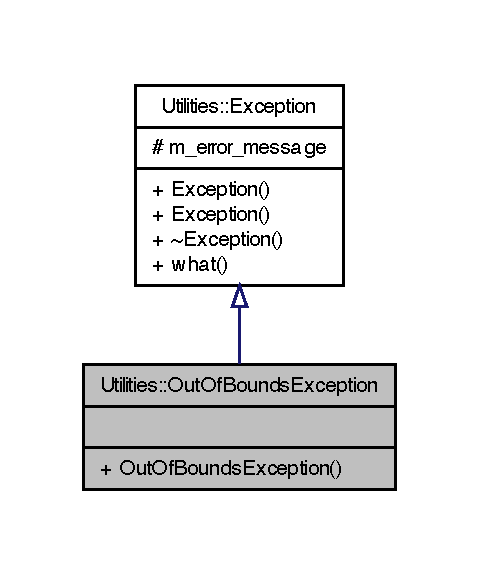
\includegraphics[width=230pt]{class_utilities_1_1_out_of_bounds_exception__coll__graph}
\end{center}
\end{figure}
\subsection*{Public Member Functions}
\begin{DoxyCompactItemize}
\item 
\hyperlink{class_utilities_1_1_out_of_bounds_exception_abd1db91b35e5b7b165ebdde59ff40b39}{OutOfBoundsException} (const char $\ast$aFileName=0, const char $\ast$aFunctionName=0, int anErrorLine=0)
\begin{DoxyCompactList}\small\item\em Default constructor. \end{DoxyCompactList}\end{DoxyCompactItemize}


\subsection{Detailed Description}


Definition at line 56 of file OutOfBoundsException.h.



\subsection{Constructor \& Destructor Documentation}
\hypertarget{class_utilities_1_1_out_of_bounds_exception_abd1db91b35e5b7b165ebdde59ff40b39}{
\index{Utilities::OutOfBoundsException@{Utilities::OutOfBoundsException}!OutOfBoundsException@{OutOfBoundsException}}
\index{OutOfBoundsException@{OutOfBoundsException}!Utilities::OutOfBoundsException@{Utilities::OutOfBoundsException}}
\subsubsection[{OutOfBoundsException}]{\setlength{\rightskip}{0pt plus 5cm}Utilities::OutOfBoundsException::OutOfBoundsException (
\begin{DoxyParamCaption}
\item[{const char $\ast$}]{aFileName = {\ttfamily 0}, }
\item[{const char $\ast$}]{aFunctionName = {\ttfamily 0}, }
\item[{int}]{anErrorLine = {\ttfamily 0}}
\end{DoxyParamCaption}
)\hspace{0.3cm}{\ttfamily  \mbox{[}inline\mbox{]}}}}
\label{class_utilities_1_1_out_of_bounds_exception_abd1db91b35e5b7b165ebdde59ff40b39}


Default constructor. 


\begin{DoxyParams}{Parameters}
{\em aFileName,:} & name of the source file where the exception was thrown (default value: 0) \\
\hline
{\em aFunctionName,:} & name of the function where the exception was thrown (default value: 0) \\
\hline
{\em anErrorLine,:} & name at which the exception was thrown (default value: 0) \\
\hline
\end{DoxyParams}


Definition at line 37 of file OutOfBoundsException.inl.



The documentation for this class was generated from the following files:\begin{DoxyCompactItemize}
\item 
/Users/fpvidal/Documents/gvirtualxray-\/code/trunk/include/gVirtualXRay/\hyperlink{_out_of_bounds_exception_8h}{OutOfBoundsException.h}\item 
/Users/fpvidal/Documents/gvirtualxray-\/code/trunk/include/gVirtualXRay/\hyperlink{_out_of_bounds_exception_8inl}{OutOfBoundsException.inl}\end{DoxyCompactItemize}

\hypertarget{class_utilities_1_1_out_of_memory_exception}{
\section{Utilities::OutOfMemoryException Class Reference}
\label{class_utilities_1_1_out_of_memory_exception}\index{Utilities::OutOfMemoryException@{Utilities::OutOfMemoryException}}
}


\hyperlink{class_utilities_1_1_out_of_memory_exception}{OutOfMemoryException} is a class to handle exceptions when accessing an array cell that is not accessible, i.e. out of bounds memory access.  




{\ttfamily \#include $<$OutOfMemoryException.h$>$}



Inheritance diagram for Utilities::OutOfMemoryException:\nopagebreak
\begin{figure}[H]
\begin{center}
\leavevmode
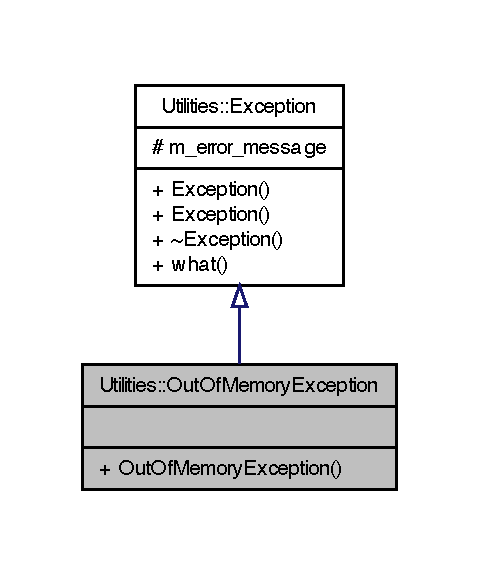
\includegraphics[width=230pt]{class_utilities_1_1_out_of_memory_exception__inherit__graph}
\end{center}
\end{figure}


Collaboration diagram for Utilities::OutOfMemoryException:\nopagebreak
\begin{figure}[H]
\begin{center}
\leavevmode
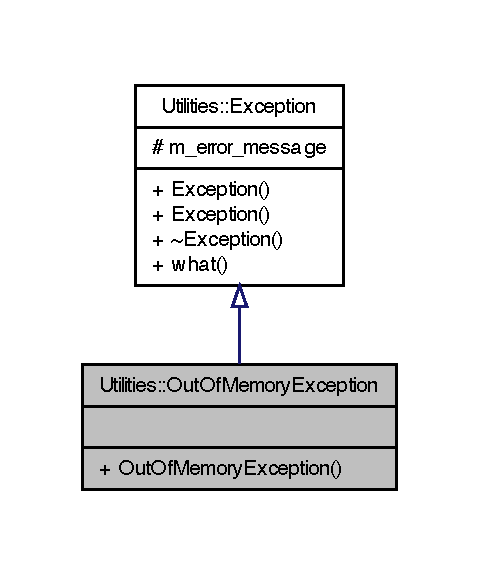
\includegraphics[width=230pt]{class_utilities_1_1_out_of_memory_exception__coll__graph}
\end{center}
\end{figure}
\subsection*{Public Member Functions}
\begin{DoxyCompactItemize}
\item 
\hyperlink{class_utilities_1_1_out_of_memory_exception_a9f10331b987f010273715db077aa4403}{OutOfMemoryException} (const char $\ast$aFileName=0, const char $\ast$aFunctionName=0, int anErrorLine=0)
\begin{DoxyCompactList}\small\item\em Default constructor. \end{DoxyCompactList}\end{DoxyCompactItemize}


\subsection{Detailed Description}
\hyperlink{class_utilities_1_1_out_of_memory_exception}{OutOfMemoryException} is a class to handle exceptions when accessing an array cell that is not accessible, i.e. out of bounds memory access. 

\hyperlink{class_utilities_1_1_out_of_memory_exception}{OutOfMemoryException} is a class to handle exceptions when memory cannot be allocated dynamically. 

Definition at line 55 of file OutOfMemoryException.h.



\subsection{Constructor \& Destructor Documentation}
\hypertarget{class_utilities_1_1_out_of_memory_exception_a9f10331b987f010273715db077aa4403}{
\index{Utilities::OutOfMemoryException@{Utilities::OutOfMemoryException}!OutOfMemoryException@{OutOfMemoryException}}
\index{OutOfMemoryException@{OutOfMemoryException}!Utilities::OutOfMemoryException@{Utilities::OutOfMemoryException}}
\subsubsection[{OutOfMemoryException}]{\setlength{\rightskip}{0pt plus 5cm}Utilities::OutOfMemoryException::OutOfMemoryException (
\begin{DoxyParamCaption}
\item[{const char $\ast$}]{aFileName = {\ttfamily 0}, }
\item[{const char $\ast$}]{aFunctionName = {\ttfamily 0}, }
\item[{int}]{anErrorLine = {\ttfamily 0}}
\end{DoxyParamCaption}
)\hspace{0.3cm}{\ttfamily  \mbox{[}inline\mbox{]}}}}
\label{class_utilities_1_1_out_of_memory_exception_a9f10331b987f010273715db077aa4403}


Default constructor. 


\begin{DoxyParams}{Parameters}
{\em aFileName,:} & name of the source file where the exception was thrown (default value: 0) \\
\hline
{\em aFunctionName,:} & name of the function where the exception was thrown (default value: 0) \\
\hline
{\em anErrorLine,:} & name at which the exception was thrown (default value: 0) \\
\hline
\end{DoxyParams}


Definition at line 37 of file OutOfMemoryException.inl.



The documentation for this class was generated from the following files:\begin{DoxyCompactItemize}
\item 
/Users/fpvidal/Documents/gvirtualxray-\/code/trunk/include/gVirtualXRay/\hyperlink{_out_of_memory_exception_8h}{OutOfMemoryException.h}\item 
/Users/fpvidal/Documents/gvirtualxray-\/code/trunk/include/gVirtualXRay/\hyperlink{_out_of_memory_exception_8inl}{OutOfMemoryException.inl}\end{DoxyCompactItemize}

\hypertarget{class_graphics_1_1_polygon_mesh}{
\section{Graphics::PolygonMesh Class Reference}
\label{class_graphics_1_1_polygon_mesh}\index{Graphics::PolygonMesh@{Graphics::PolygonMesh}}
}


\hyperlink{class_graphics_1_1_polygon_mesh}{PolygonMesh} is a class to handle polygon (triangles or quads) meshes.  




{\ttfamily \#include $<$PolygonMesh.h$>$}



Inheritance diagram for Graphics::PolygonMesh:
\nopagebreak
\begin{figure}[H]
\begin{center}
\leavevmode
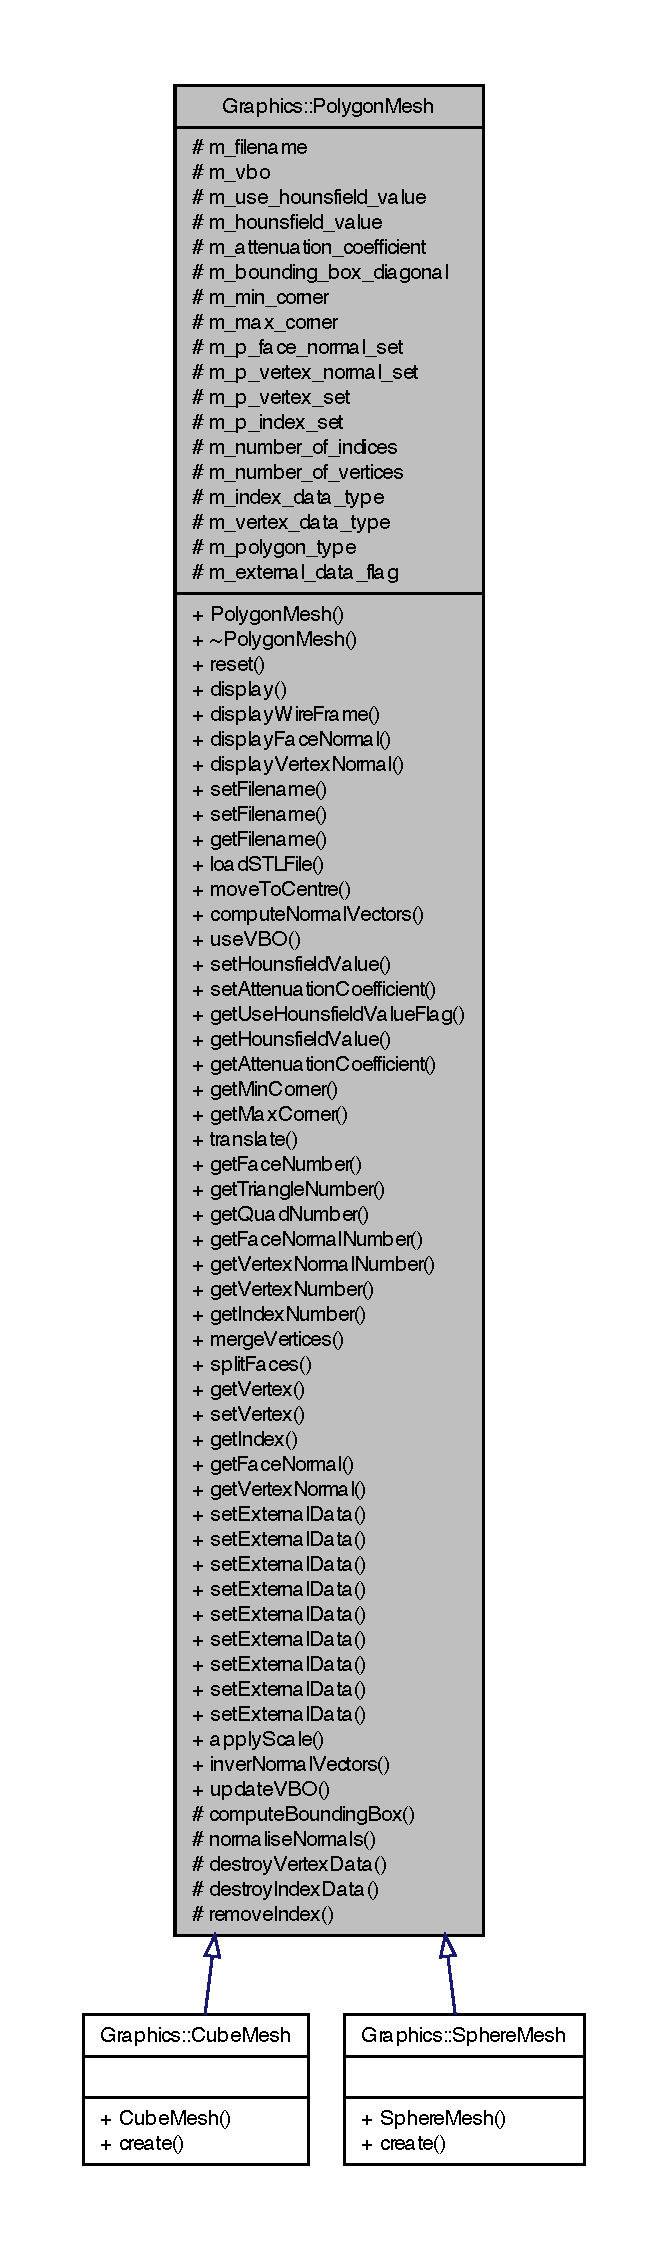
\includegraphics[height=600pt]{class_graphics_1_1_polygon_mesh__inherit__graph}
\end{center}
\end{figure}


Collaboration diagram for Graphics::PolygonMesh:
\nopagebreak
\begin{figure}[H]
\begin{center}
\leavevmode
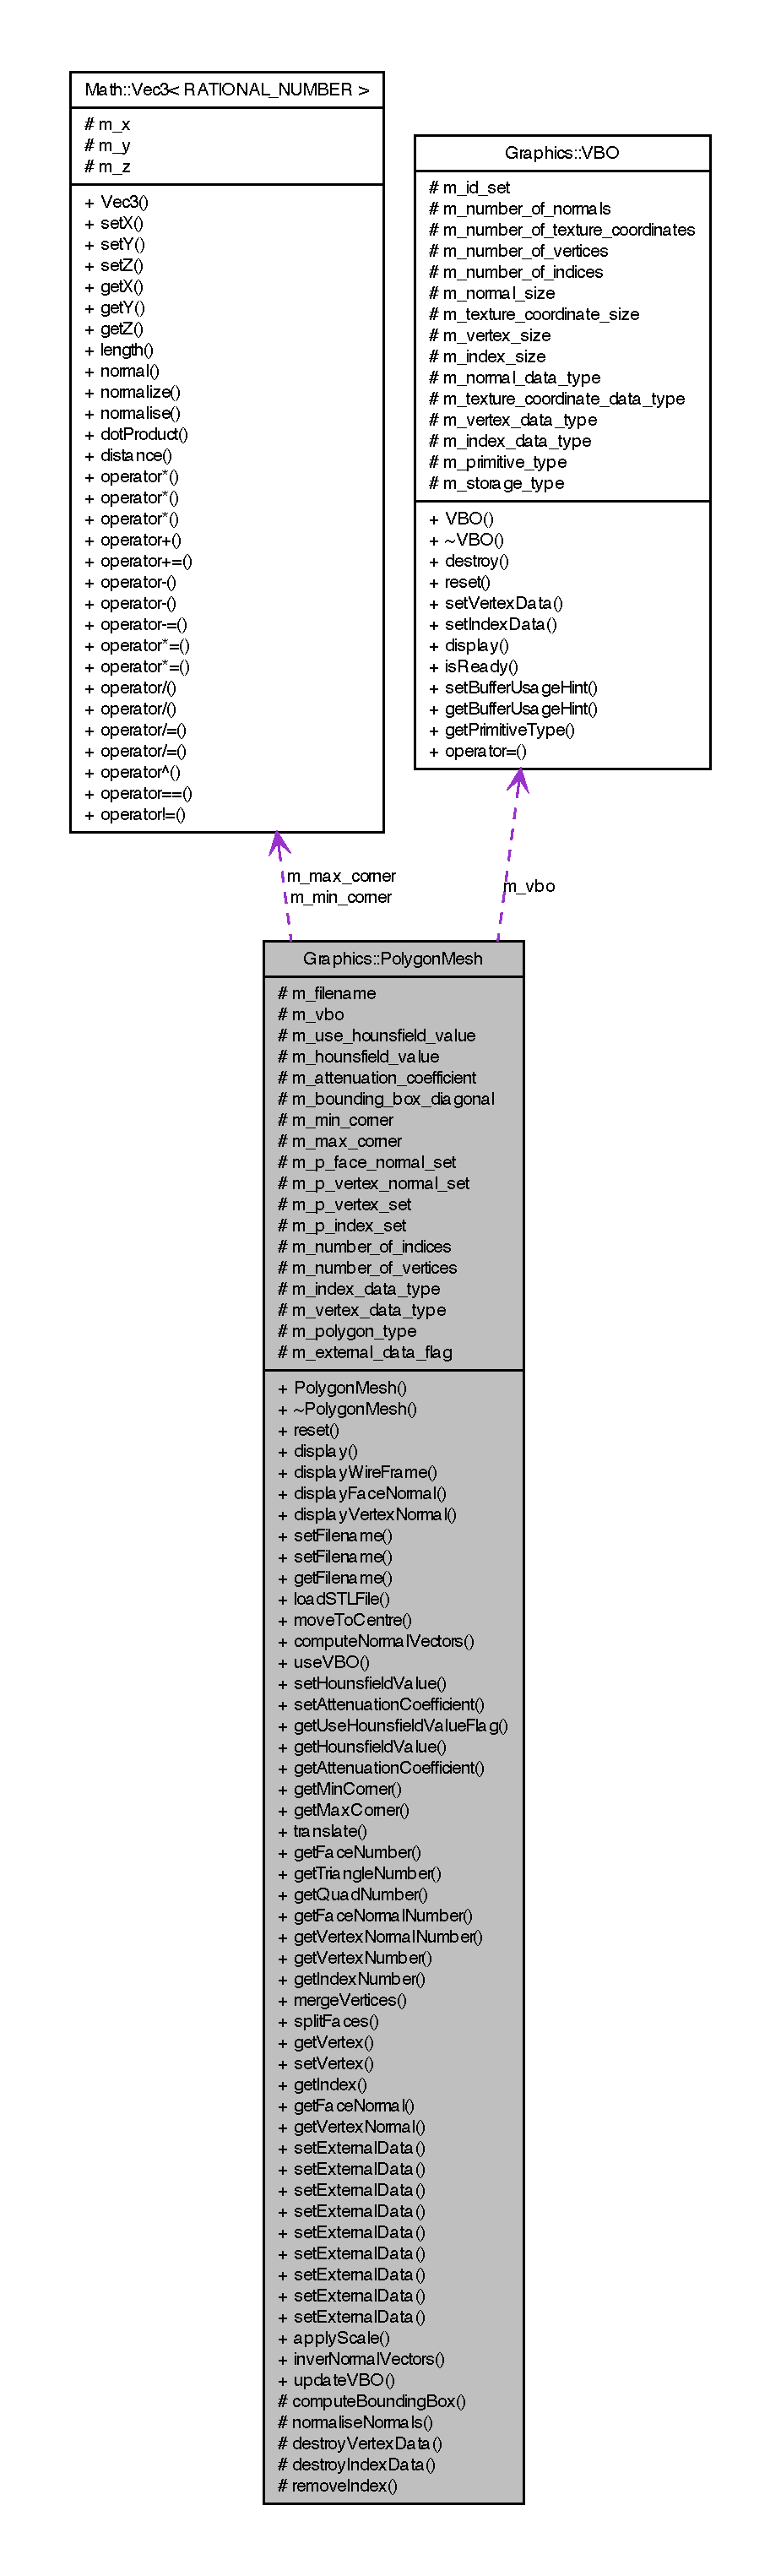
\includegraphics[height=600pt]{class_graphics_1_1_polygon_mesh__coll__graph}
\end{center}
\end{figure}
\subsection*{Public Member Functions}
\begin{DoxyCompactItemize}
\item 
\hyperlink{class_graphics_1_1_polygon_mesh_a4a74b31e7615591ec53fb2954617a469}{PolygonMesh} ()
\begin{DoxyCompactList}\small\item\em Default constructor. \end{DoxyCompactList}\item 
\hyperlink{class_graphics_1_1_polygon_mesh_a61906b1f357df6a465202775e4b32aa0}{$\sim$PolygonMesh} ()
\begin{DoxyCompactList}\small\item\em Destructor. \end{DoxyCompactList}\item 
void \hyperlink{class_graphics_1_1_polygon_mesh_a1ff9fbdc31bf7b0c86176b5e99fabd14}{reset} ()
\begin{DoxyCompactList}\small\item\em Reset the data. \end{DoxyCompactList}\item 
void \hyperlink{class_graphics_1_1_polygon_mesh_a0f15277a3f50841998066657a4c3bc41}{display} ()
\begin{DoxyCompactList}\small\item\em Display the triangular mesh using OpenGL. \end{DoxyCompactList}\item 
void \hyperlink{class_graphics_1_1_polygon_mesh_a60a14fd59728ad30a68829bf1647a7f0}{displayWireFrame} ()
\begin{DoxyCompactList}\small\item\em Display the triangular mesh in wireframe using OpenGL. \end{DoxyCompactList}\item 
void \hyperlink{class_graphics_1_1_polygon_mesh_a380deb98652eccfbc3cb577a1a9e1b7a}{displayFaceNormal} (\hyperlink{namespace_utilities_a40969b96bd8d847b962e297cb79f08ce}{RATIONAL\_\-NUMBER} aNormalSize=0.5 $\ast$cm) const 
\begin{DoxyCompactList}\small\item\em Display the face normal vectors. \end{DoxyCompactList}\item 
void \hyperlink{class_graphics_1_1_polygon_mesh_aedad6cac01ba1cd566bdc81dc864f64b}{displayVertexNormal} (\hyperlink{namespace_utilities_a40969b96bd8d847b962e297cb79f08ce}{RATIONAL\_\-NUMBER} aNormalSize=0.5 $\ast$cm) const 
\begin{DoxyCompactList}\small\item\em Display the vertex normal vectors. \end{DoxyCompactList}\item 
void \hyperlink{class_graphics_1_1_polygon_mesh_a7af702f04a87789219f5c5373582c7d3}{setFilename} (const char $\ast$aFilename)
\begin{DoxyCompactList}\small\item\em Set the name of the file that contains the polygon mesh. \end{DoxyCompactList}\item 
void \hyperlink{class_graphics_1_1_polygon_mesh_a12051c2f6c3308d729a608cca650ff14}{setFilename} (const std::string \&aFilename)
\begin{DoxyCompactList}\small\item\em Set the name of the file that contains the polygon mesh. \end{DoxyCompactList}\item 
const std::string \& \hyperlink{class_graphics_1_1_polygon_mesh_a2bbcd8e618e1698f79eb7a8996e7a646}{getFilename} () const 
\begin{DoxyCompactList}\small\item\em Accessor on the name of the file that contains the polygon mesh. \end{DoxyCompactList}\item 
void \hyperlink{class_graphics_1_1_polygon_mesh_a3a2d83e615dc381d4cc45e0a5551725a}{loadSTLFile} (bool aMoveToCentreFlag, bool anAutoComputeNormalFlag, bool aPrintDebugInfoFlag, bool aCreateVBOFlag, \hyperlink{namespace_utilities_a40969b96bd8d847b962e297cb79f08ce}{RATIONAL\_\-NUMBER} aScale, int aBufferUsageHing)
\begin{DoxyCompactList}\small\item\em Set the name of the file that contains the polygon mesh. \end{DoxyCompactList}\item 
void \hyperlink{class_graphics_1_1_polygon_mesh_a26f0e68845c9f24896d8156ff72e747a}{moveToCentre} ()
\begin{DoxyCompactList}\small\item\em Move the polygon to the center. \end{DoxyCompactList}\item 
void \hyperlink{class_graphics_1_1_polygon_mesh_ad5841a84e5c7c794010bc87ad65694e0}{computeNormalVectors} ()
\begin{DoxyCompactList}\small\item\em Compute the normal vectors using the cross product method. \end{DoxyCompactList}\item 
bool \hyperlink{class_graphics_1_1_polygon_mesh_a790ef6e4861d98228830170f0217661b}{useVBO} (int aBufferUsageHing, int aTypeOfPrimitive)
\begin{DoxyCompactList}\small\item\em Use a vertex buffer object if possible. \end{DoxyCompactList}\item 
void \hyperlink{class_graphics_1_1_polygon_mesh_a2fb399af8869e1989e25c3eadb101c02}{setHounsfieldValue} (const \hyperlink{namespace_utilities_a40969b96bd8d847b962e297cb79f08ce}{RATIONAL\_\-NUMBER} \&aHounsfieldValue)
\begin{DoxyCompactList}\small\item\em Set the Hounsfield value of the object material. \end{DoxyCompactList}\item 
void \hyperlink{class_graphics_1_1_polygon_mesh_ad32af6aa79c5822729ac48cced78e477}{setAttenuationCoefficient} (const \hyperlink{namespace_utilities_a40969b96bd8d847b962e297cb79f08ce}{RATIONAL\_\-NUMBER} \&anAttenuationCoefficient)
\begin{DoxyCompactList}\small\item\em Set the attenuation coefficient of the object material. \end{DoxyCompactList}\item 
bool \hyperlink{class_graphics_1_1_polygon_mesh_ad04b48ad09e20ecbfbf9d5c97331ef90}{getUseHounsfieldValueFlag} () const 
\item 
\hyperlink{namespace_utilities_a40969b96bd8d847b962e297cb79f08ce}{RATIONAL\_\-NUMBER} \hyperlink{class_graphics_1_1_polygon_mesh_a81fdfafcb621af66d7d9333ba5684491}{getHounsfieldValue} () const 
\begin{DoxyCompactList}\small\item\em Accessor on the Hounsfield value. \end{DoxyCompactList}\item 
\hyperlink{namespace_utilities_a40969b96bd8d847b962e297cb79f08ce}{RATIONAL\_\-NUMBER} \hyperlink{class_graphics_1_1_polygon_mesh_a5d19970ad39b804d00be1eff20c31365}{getAttenuationCoefficient} () const 
\begin{DoxyCompactList}\small\item\em Accessor on the attenuation coefficient. \end{DoxyCompactList}\item 
const \hyperlink{class_math_1_1_vec3}{VEC3} \& \hyperlink{class_graphics_1_1_polygon_mesh_a573df0163340b2e7b8dcdd2b1caea790}{getMinCorner} () const 
\begin{DoxyCompactList}\small\item\em Accessor on the bounding box lower corner. \end{DoxyCompactList}\item 
const \hyperlink{class_math_1_1_vec3}{VEC3} \& \hyperlink{class_graphics_1_1_polygon_mesh_a23a7b423d853e16d043bb125161afcb0}{getMaxCorner} () const 
\begin{DoxyCompactList}\small\item\em Accessor on the bounding box upper corner. \end{DoxyCompactList}\item 
void \hyperlink{class_graphics_1_1_polygon_mesh_a4094c55d1009da88fb834e0957340c7c}{translate} (const \hyperlink{class_math_1_1_vec3}{VEC3} \&aTranslationVector)
\begin{DoxyCompactList}\small\item\em Use a vertex buffer object if possible. \end{DoxyCompactList}\item 
unsigned int \hyperlink{class_graphics_1_1_polygon_mesh_aa19d5b1760ae65457d646d4e6558dc43}{getFaceNumber} () const 
\begin{DoxyCompactList}\small\item\em Accessor on the number of faces. \end{DoxyCompactList}\item 
unsigned int \hyperlink{class_graphics_1_1_polygon_mesh_afea2475f1eb3e88bac083a2f79d3bb19}{getTriangleNumber} () const 
\begin{DoxyCompactList}\small\item\em Accessor on the number of triangles. \end{DoxyCompactList}\item 
unsigned int \hyperlink{class_graphics_1_1_polygon_mesh_a09109f7c34075d12c9837a183cc120ca}{getQuadNumber} () const 
\begin{DoxyCompactList}\small\item\em Accessor on the number of quads. \end{DoxyCompactList}\item 
unsigned int \hyperlink{class_graphics_1_1_polygon_mesh_a2848ccf95a11afb1912b760dd8fb85da}{getFaceNormalNumber} () const 
\begin{DoxyCompactList}\small\item\em Accessor on the number of face normal vectors. \end{DoxyCompactList}\item 
unsigned int \hyperlink{class_graphics_1_1_polygon_mesh_ac0d769a296df3f78a918f63f04bce338}{getVertexNormalNumber} () const 
\begin{DoxyCompactList}\small\item\em Accessor on the number of vertex normal vectors. \end{DoxyCompactList}\item 
unsigned int \hyperlink{class_graphics_1_1_polygon_mesh_aaca647be2d7c9e9168915c106cc6a162}{getVertexNumber} () const 
\begin{DoxyCompactList}\small\item\em Accessor on the number of vertices. \end{DoxyCompactList}\item 
unsigned int \hyperlink{class_graphics_1_1_polygon_mesh_af7b8cf4fd0544ceeabe2b97b85893314}{getIndexNumber} () const 
\begin{DoxyCompactList}\small\item\em Accessor on the number of indices. \end{DoxyCompactList}\item 
void \hyperlink{class_graphics_1_1_polygon_mesh_a4eabb8a7f457991de920d772c9b72745}{mergeVertices} (bool aPrintDebugInfoFlag=false)
\item 
void \hyperlink{class_graphics_1_1_polygon_mesh_a7e12700ce99e0c122e72d4897bd64f95}{splitFaces} (bool aPrintDebugInfoFlag=false)
\begin{DoxyCompactList}\small\item\em Split each face into four faces. \end{DoxyCompactList}\item 
\hyperlink{class_math_1_1_vec3}{VEC3} \hyperlink{class_graphics_1_1_polygon_mesh_a9fd98d97b7ce3585fa1af572002cc27c}{getVertex} (unsigned int anIndex) const 
\begin{DoxyCompactList}\small\item\em Accessor on a given vertex. \end{DoxyCompactList}\item 
void \hyperlink{class_graphics_1_1_polygon_mesh_a700da528621a371bb989cfb2fa39b49e}{setVertex} (unsigned int anIndex, const \hyperlink{class_math_1_1_vec3}{VEC3} \&aVertex)
\begin{DoxyCompactList}\small\item\em Change the value of a given vertex. \end{DoxyCompactList}\item 
int \hyperlink{class_graphics_1_1_polygon_mesh_a32645e7e4b5303bcf4b9fa63efe86a98}{getIndex} (unsigned int anIndex) const 
\begin{DoxyCompactList}\small\item\em Accessor on a given index. \end{DoxyCompactList}\item 
\hyperlink{class_math_1_1_vec3}{VEC3} \hyperlink{class_graphics_1_1_polygon_mesh_a6d10e50e17b7e8c036d3a2a6ff6f9985}{getFaceNormal} (unsigned int anIndex) const 
\begin{DoxyCompactList}\small\item\em Accessor on a given face normal. \end{DoxyCompactList}\item 
\hyperlink{class_math_1_1_vec3}{VEC3} \hyperlink{class_graphics_1_1_polygon_mesh_a0c3e461c151fed4744ca59f19fbdd1ee}{getVertexNormal} (unsigned int anIndex) const 
\begin{DoxyCompactList}\small\item\em Accessor on a given vertex normal. \end{DoxyCompactList}\item 
void \hyperlink{class_graphics_1_1_polygon_mesh_a406d0b1a01b93e5da19d9617f9b21d16}{setExternalData} (int aPolygonType, const void $\ast$aVertexArray, unsigned int aNumberOfVertices, int aVertexDataType, const void $\ast$anIndexArray, unsigned int aNumberOfIndices, int anIndexDataType, bool aCreateVBOFlag, int aTypeOfVBO)
\item 
void \hyperlink{class_graphics_1_1_polygon_mesh_ae0a83f6105c1913081905318530697e2}{setExternalData} (int aPolygonType, const std::vector$<$ float $>$ $\ast$aVertexArray, bool aCreateVBOFlag, int aTypeOfVBO)
\item 
void \hyperlink{class_graphics_1_1_polygon_mesh_a4e54503d4fd75b586d13a4933a338601}{setExternalData} (int aPolygonType, const std::vector$<$ double $>$ $\ast$aVertexArray, bool aCreateVBOFlag, int aTypeOfVBO)
\item 
void \hyperlink{class_graphics_1_1_polygon_mesh_a02beb66b179ae5fa5f94b9ab563a04b8}{setExternalData} (int aPolygonType, const std::vector$<$ float $>$ $\ast$aVertexArray, const std::vector$<$ unsigned int $>$ $\ast$anIndexArray, bool aCreateVBOFlag, int aTypeOfVBO)
\item 
void \hyperlink{class_graphics_1_1_polygon_mesh_ae324bf6ce3f7ad3d50bdd10d565e639f}{setExternalData} (int aPolygonType, const std::vector$<$ double $>$ $\ast$aVertexArray, const std::vector$<$ unsigned int $>$ $\ast$anIndexArray, bool aCreateVBOFlag, int aTypeOfVBO)
\item 
void \hyperlink{class_graphics_1_1_polygon_mesh_a87fbf60171fc7befac1580256688a35c}{setExternalData} (int aPolygonType, const std::vector$<$ float $>$ $\ast$aVertexArray, const std::vector$<$ unsigned short $>$ $\ast$anIndexArray, bool aCreateVBOFlag, int aTypeOfVBO)
\item 
void \hyperlink{class_graphics_1_1_polygon_mesh_ad9b8e4f262f0f71c6e81c94e65abbd34}{setExternalData} (int aPolygonType, const std::vector$<$ double $>$ $\ast$aVertexArray, const std::vector$<$ unsigned short $>$ $\ast$anIndexArray, bool aCreateVBOFlag, int aTypeOfVBO)
\item 
void \hyperlink{class_graphics_1_1_polygon_mesh_a72789f03fd9d13ea564d61293c26aeaa}{setExternalData} (int aPolygonType, const std::vector$<$ float $>$ $\ast$aVertexArray, const std::vector$<$ unsigned char $>$ $\ast$anIndexArray, bool aCreateVBOFlag, int aTypeOfVBO)
\item 
void \hyperlink{class_graphics_1_1_polygon_mesh_aaaf9a96ac048c5d646de2bd5fad70390}{setExternalData} (int aPolygonType, const std::vector$<$ double $>$ $\ast$aVertexArray, const std::vector$<$ unsigned char $>$ $\ast$anIndexArray, bool aCreateVBOFlag, int aTypeOfVBO)
\item 
void \hyperlink{class_graphics_1_1_polygon_mesh_a6d2c8f160f1b8546dc32810aa97c0df6}{applyScale} (const \hyperlink{namespace_utilities_a40969b96bd8d847b962e297cb79f08ce}{RATIONAL\_\-NUMBER} \&aScale)
\item 
void \hyperlink{class_graphics_1_1_polygon_mesh_ab587ef84af5f44366b4c6e170aa35ea0}{inverNormalVectors} ()
\begin{DoxyCompactList}\small\item\em Inverse the normal vectors. \end{DoxyCompactList}\item 
virtual void \hyperlink{class_graphics_1_1_polygon_mesh_aee125712037722cbf8a2131017c2d662}{updateVBO} (int aTypeOfVBO, int aTypeOfPrimitive)
\begin{DoxyCompactList}\small\item\em Update the \hyperlink{class_graphics_1_1_v_b_o}{VBO}. \end{DoxyCompactList}\end{DoxyCompactItemize}
\subsection*{Protected Member Functions}
\begin{DoxyCompactItemize}
\item 
void \hyperlink{class_graphics_1_1_polygon_mesh_a2c4bbe3f05df1d4e49214a10895c03a2}{computeBoundingBox} ()
\begin{DoxyCompactList}\small\item\em Update the bounding box. \end{DoxyCompactList}\item 
void \hyperlink{class_graphics_1_1_polygon_mesh_ac0625fa4506cab4d42f3f83f332912d9}{normaliseNormals} ()
\begin{DoxyCompactList}\small\item\em Normalise the normal vectors. \end{DoxyCompactList}\item 
void \hyperlink{class_graphics_1_1_polygon_mesh_acab2607f9049bd014aa832476bb9639f}{destroyVertexData} ()
\begin{DoxyCompactList}\small\item\em Release the memory held by the vertex data if needed. \end{DoxyCompactList}\item 
void \hyperlink{class_graphics_1_1_polygon_mesh_aef6d6127e866fce09c2245550a518a9c}{destroyIndexData} ()
\begin{DoxyCompactList}\small\item\em Release the memory held by the index data if needed. \end{DoxyCompactList}\item 
void \hyperlink{class_graphics_1_1_polygon_mesh_af10ea58e6dd63cd085662ae255c26054}{removeIndex} (bool aPrintDebugInfoFlag=false)
\begin{DoxyCompactList}\small\item\em Remove the index. \end{DoxyCompactList}\end{DoxyCompactItemize}
\subsection*{Protected Attributes}
\begin{DoxyCompactItemize}
\item 
std::string \hyperlink{class_graphics_1_1_polygon_mesh_a455483e27861ed72beacd76e70c438bb}{m\_\-filename}
\begin{DoxyCompactList}\small\item\em Name of the file that contains the polygon mesh. \end{DoxyCompactList}\item 
\hyperlink{class_graphics_1_1_v_b_o}{VBO} \hyperlink{class_graphics_1_1_polygon_mesh_a181beb08c7c8b9a42666b948ed48f6da}{m\_\-vbo}
\begin{DoxyCompactList}\small\item\em Vertex buffer object. \end{DoxyCompactList}\item 
bool \hyperlink{class_graphics_1_1_polygon_mesh_a5c193c50619f85408f295c8c0a5e43a6}{m\_\-use\_\-hounsfield\_\-value}
\begin{DoxyCompactList}\small\item\em Flag about the use of the Hounsfield value or attenuation coefficient. \end{DoxyCompactList}\item 
\hyperlink{namespace_utilities_a40969b96bd8d847b962e297cb79f08ce}{RATIONAL\_\-NUMBER} \hyperlink{class_graphics_1_1_polygon_mesh_a2c2e3ac536ecf140a464fe074b4a6cb0}{m\_\-hounsfield\_\-value}
\begin{DoxyCompactList}\small\item\em Hounsfield value. \end{DoxyCompactList}\item 
\hyperlink{namespace_utilities_a40969b96bd8d847b962e297cb79f08ce}{RATIONAL\_\-NUMBER} \hyperlink{class_graphics_1_1_polygon_mesh_ab1ca7c29c40e562b58ff4915e26724cb}{m\_\-attenuation\_\-coefficient}
\begin{DoxyCompactList}\small\item\em Attenuation coefficient. \end{DoxyCompactList}\item 
\hyperlink{namespace_utilities_a40969b96bd8d847b962e297cb79f08ce}{RATIONAL\_\-NUMBER} \hyperlink{class_graphics_1_1_polygon_mesh_aaa93546b5f9f1f9ddb70aaeeb2ed5be8}{m\_\-bounding\_\-box\_\-diagonal}
\begin{DoxyCompactList}\small\item\em Length of the bounding box diagonal. \end{DoxyCompactList}\item 
\hyperlink{class_math_1_1_vec3}{VEC3} \hyperlink{class_graphics_1_1_polygon_mesh_a15afbd27c9bc4138d6b820a410401d16}{m\_\-min\_\-corner}
\begin{DoxyCompactList}\small\item\em Lower corner of the bounding box. \end{DoxyCompactList}\item 
\hyperlink{class_math_1_1_vec3}{VEC3} \hyperlink{class_graphics_1_1_polygon_mesh_a0a315335b8e97b4a533308365817660d}{m\_\-max\_\-corner}
\begin{DoxyCompactList}\small\item\em Upper corner of the bounding box. \end{DoxyCompactList}\item 
std::vector$<$ \hyperlink{namespace_utilities_a40969b96bd8d847b962e297cb79f08ce}{RATIONAL\_\-NUMBER} $>$ \hyperlink{class_graphics_1_1_polygon_mesh_a737a511ebb529e1abbb58301c9889247}{m\_\-p\_\-face\_\-normal\_\-set}
\begin{DoxyCompactList}\small\item\em Array containing the normal vectors (one per triangle) \end{DoxyCompactList}\item 
std::vector$<$ \hyperlink{namespace_utilities_a40969b96bd8d847b962e297cb79f08ce}{RATIONAL\_\-NUMBER} $>$ \hyperlink{class_graphics_1_1_polygon_mesh_aab6df25fff511d684579ca76d026fcf2}{m\_\-p\_\-vertex\_\-normal\_\-set}
\begin{DoxyCompactList}\small\item\em Array containing the normal vectors (one per vertex) \end{DoxyCompactList}\item 
void $\ast$ \hyperlink{class_graphics_1_1_polygon_mesh_ae577b2b3640a376042681a02008c6e39}{m\_\-p\_\-vertex\_\-set}
\begin{DoxyCompactList}\small\item\em Array containing the vertices. \end{DoxyCompactList}\item 
void $\ast$ \hyperlink{class_graphics_1_1_polygon_mesh_a0065f5a4a8e996c1b6da44778e978953}{m\_\-p\_\-index\_\-set}
\begin{DoxyCompactList}\small\item\em Array containing the index. \end{DoxyCompactList}\item 
unsigned int \hyperlink{class_graphics_1_1_polygon_mesh_a15c785b7d751c4876cd46c6788d411da}{m\_\-number\_\-of\_\-indices}
\begin{DoxyCompactList}\small\item\em Number of indices. \end{DoxyCompactList}\item 
unsigned int \hyperlink{class_graphics_1_1_polygon_mesh_a18eea30ed69a85cea0702e365d586176}{m\_\-number\_\-of\_\-vertices}
\begin{DoxyCompactList}\small\item\em Number of vertices. \end{DoxyCompactList}\item 
int \hyperlink{class_graphics_1_1_polygon_mesh_acf9a781bb8d8b4a3905f41bea954e83d}{m\_\-index\_\-data\_\-type}
\begin{DoxyCompactList}\small\item\em Data type of the index data; valid values are GL\_\-UNSIGNED\_\-INT, GL\_\-UNSIGNED\_\-SHORT, GL\_\-UNSIGNED\_\-BYTE and GL\_\-NONE. \end{DoxyCompactList}\item 
int \hyperlink{class_graphics_1_1_polygon_mesh_aada40563d8efefb4cddec11ee124fdb7}{m\_\-vertex\_\-data\_\-type}
\begin{DoxyCompactList}\small\item\em Data type of the vertex data; valid values are GL\_\-FLOAT, GL\_\-DOUBLE and GL\_\-NONE. \end{DoxyCompactList}\item 
int \hyperlink{class_graphics_1_1_polygon_mesh_ac435c5305cb26572409a98779e66b0f2}{m\_\-polygon\_\-type}
\begin{DoxyCompactList}\small\item\em Polygon type; valid values are GL\_\-QUADS, and GL\_\-TRIANGLES. \end{DoxyCompactList}\item 
bool \hyperlink{class_graphics_1_1_polygon_mesh_a62bdefdd8c44bcc211f4472a756e835f}{m\_\-external\_\-data\_\-flag}
\end{DoxyCompactItemize}


\subsection{Detailed Description}
\hyperlink{class_graphics_1_1_polygon_mesh}{PolygonMesh} is a class to handle polygon (triangles or quads) meshes. 

Definition at line 68 of file PolygonMesh.h.



\subsection{Constructor \& Destructor Documentation}
\hypertarget{class_graphics_1_1_polygon_mesh_a4a74b31e7615591ec53fb2954617a469}{
\index{Graphics::PolygonMesh@{Graphics::PolygonMesh}!PolygonMesh@{PolygonMesh}}
\index{PolygonMesh@{PolygonMesh}!Graphics::PolygonMesh@{Graphics::PolygonMesh}}
\subsubsection[{PolygonMesh}]{\setlength{\rightskip}{0pt plus 5cm}Graphics::PolygonMesh::PolygonMesh (
\begin{DoxyParamCaption}
{}
\end{DoxyParamCaption}
)}}
\label{class_graphics_1_1_polygon_mesh_a4a74b31e7615591ec53fb2954617a469}


Default constructor. 

\hypertarget{class_graphics_1_1_polygon_mesh_a61906b1f357df6a465202775e4b32aa0}{
\index{Graphics::PolygonMesh@{Graphics::PolygonMesh}!$\sim$PolygonMesh@{$\sim$PolygonMesh}}
\index{$\sim$PolygonMesh@{$\sim$PolygonMesh}!Graphics::PolygonMesh@{Graphics::PolygonMesh}}
\subsubsection[{$\sim$PolygonMesh}]{\setlength{\rightskip}{0pt plus 5cm}Graphics::PolygonMesh::$\sim$PolygonMesh (
\begin{DoxyParamCaption}
{}
\end{DoxyParamCaption}
)\hspace{0.3cm}{\ttfamily  \mbox{[}inline\mbox{]}}}}
\label{class_graphics_1_1_polygon_mesh_a61906b1f357df6a465202775e4b32aa0}


Destructor. 



Definition at line 52 of file PolygonMesh.inl.



\subsection{Member Function Documentation}
\hypertarget{class_graphics_1_1_polygon_mesh_a6d2c8f160f1b8546dc32810aa97c0df6}{
\index{Graphics::PolygonMesh@{Graphics::PolygonMesh}!applyScale@{applyScale}}
\index{applyScale@{applyScale}!Graphics::PolygonMesh@{Graphics::PolygonMesh}}
\subsubsection[{applyScale}]{\setlength{\rightskip}{0pt plus 5cm}void Graphics::PolygonMesh::applyScale (
\begin{DoxyParamCaption}
\item[{const {\bf RATIONAL\_\-NUMBER} \&}]{aScale}
\end{DoxyParamCaption}
)\hspace{0.3cm}{\ttfamily  \mbox{[}inline\mbox{]}}}}
\label{class_graphics_1_1_polygon_mesh_a6d2c8f160f1b8546dc32810aa97c0df6}
Apply a scaling factor to the vertex data. Note that the bounding box will be automatically updated. 
\begin{DoxyParams}{Parameters}
{\em aScale,:} & scaling factor \\
\hline
\end{DoxyParams}


Definition at line 265 of file PolygonMesh.inl.

\hypertarget{class_graphics_1_1_polygon_mesh_a2c4bbe3f05df1d4e49214a10895c03a2}{
\index{Graphics::PolygonMesh@{Graphics::PolygonMesh}!computeBoundingBox@{computeBoundingBox}}
\index{computeBoundingBox@{computeBoundingBox}!Graphics::PolygonMesh@{Graphics::PolygonMesh}}
\subsubsection[{computeBoundingBox}]{\setlength{\rightskip}{0pt plus 5cm}void Graphics::PolygonMesh::computeBoundingBox (
\begin{DoxyParamCaption}
{}
\end{DoxyParamCaption}
)\hspace{0.3cm}{\ttfamily  \mbox{[}inline, protected\mbox{]}}}}
\label{class_graphics_1_1_polygon_mesh_a2c4bbe3f05df1d4e49214a10895c03a2}


Update the bounding box. 



Definition at line 237 of file PolygonMesh.inl.

\hypertarget{class_graphics_1_1_polygon_mesh_ad5841a84e5c7c794010bc87ad65694e0}{
\index{Graphics::PolygonMesh@{Graphics::PolygonMesh}!computeNormalVectors@{computeNormalVectors}}
\index{computeNormalVectors@{computeNormalVectors}!Graphics::PolygonMesh@{Graphics::PolygonMesh}}
\subsubsection[{computeNormalVectors}]{\setlength{\rightskip}{0pt plus 5cm}void Graphics::PolygonMesh::computeNormalVectors (
\begin{DoxyParamCaption}
{}
\end{DoxyParamCaption}
)}}
\label{class_graphics_1_1_polygon_mesh_ad5841a84e5c7c794010bc87ad65694e0}


Compute the normal vectors using the cross product method. 

\hypertarget{class_graphics_1_1_polygon_mesh_aef6d6127e866fce09c2245550a518a9c}{
\index{Graphics::PolygonMesh@{Graphics::PolygonMesh}!destroyIndexData@{destroyIndexData}}
\index{destroyIndexData@{destroyIndexData}!Graphics::PolygonMesh@{Graphics::PolygonMesh}}
\subsubsection[{destroyIndexData}]{\setlength{\rightskip}{0pt plus 5cm}void Graphics::PolygonMesh::destroyIndexData (
\begin{DoxyParamCaption}
{}
\end{DoxyParamCaption}
)\hspace{0.3cm}{\ttfamily  \mbox{[}protected\mbox{]}}}}
\label{class_graphics_1_1_polygon_mesh_aef6d6127e866fce09c2245550a518a9c}


Release the memory held by the index data if needed. 

\hypertarget{class_graphics_1_1_polygon_mesh_acab2607f9049bd014aa832476bb9639f}{
\index{Graphics::PolygonMesh@{Graphics::PolygonMesh}!destroyVertexData@{destroyVertexData}}
\index{destroyVertexData@{destroyVertexData}!Graphics::PolygonMesh@{Graphics::PolygonMesh}}
\subsubsection[{destroyVertexData}]{\setlength{\rightskip}{0pt plus 5cm}void Graphics::PolygonMesh::destroyVertexData (
\begin{DoxyParamCaption}
{}
\end{DoxyParamCaption}
)\hspace{0.3cm}{\ttfamily  \mbox{[}protected\mbox{]}}}}
\label{class_graphics_1_1_polygon_mesh_acab2607f9049bd014aa832476bb9639f}


Release the memory held by the vertex data if needed. 

\hypertarget{class_graphics_1_1_polygon_mesh_a0f15277a3f50841998066657a4c3bc41}{
\index{Graphics::PolygonMesh@{Graphics::PolygonMesh}!display@{display}}
\index{display@{display}!Graphics::PolygonMesh@{Graphics::PolygonMesh}}
\subsubsection[{display}]{\setlength{\rightskip}{0pt plus 5cm}void Graphics::PolygonMesh::display (
\begin{DoxyParamCaption}
{}
\end{DoxyParamCaption}
)}}
\label{class_graphics_1_1_polygon_mesh_a0f15277a3f50841998066657a4c3bc41}


Display the triangular mesh using OpenGL. 

\hypertarget{class_graphics_1_1_polygon_mesh_a380deb98652eccfbc3cb577a1a9e1b7a}{
\index{Graphics::PolygonMesh@{Graphics::PolygonMesh}!displayFaceNormal@{displayFaceNormal}}
\index{displayFaceNormal@{displayFaceNormal}!Graphics::PolygonMesh@{Graphics::PolygonMesh}}
\subsubsection[{displayFaceNormal}]{\setlength{\rightskip}{0pt plus 5cm}void Graphics::PolygonMesh::displayFaceNormal (
\begin{DoxyParamCaption}
\item[{{\bf RATIONAL\_\-NUMBER}}]{aNormalSize = {\ttfamily 0.5~$\ast$cm}}
\end{DoxyParamCaption}
) const}}
\label{class_graphics_1_1_polygon_mesh_a380deb98652eccfbc3cb577a1a9e1b7a}


Display the face normal vectors. 


\begin{DoxyParams}{Parameters}
{\em aNormalSize,:} & the size of the vectors (default value is 0.5 cm) \\
\hline
\end{DoxyParams}
\hypertarget{class_graphics_1_1_polygon_mesh_aedad6cac01ba1cd566bdc81dc864f64b}{
\index{Graphics::PolygonMesh@{Graphics::PolygonMesh}!displayVertexNormal@{displayVertexNormal}}
\index{displayVertexNormal@{displayVertexNormal}!Graphics::PolygonMesh@{Graphics::PolygonMesh}}
\subsubsection[{displayVertexNormal}]{\setlength{\rightskip}{0pt plus 5cm}void Graphics::PolygonMesh::displayVertexNormal (
\begin{DoxyParamCaption}
\item[{{\bf RATIONAL\_\-NUMBER}}]{aNormalSize = {\ttfamily 0.5~$\ast$cm}}
\end{DoxyParamCaption}
) const}}
\label{class_graphics_1_1_polygon_mesh_aedad6cac01ba1cd566bdc81dc864f64b}


Display the vertex normal vectors. 


\begin{DoxyParams}{Parameters}
{\em aNormalSize,:} & the size of the vectors (default value is 0.5 cm) \\
\hline
\end{DoxyParams}
\hypertarget{class_graphics_1_1_polygon_mesh_a60a14fd59728ad30a68829bf1647a7f0}{
\index{Graphics::PolygonMesh@{Graphics::PolygonMesh}!displayWireFrame@{displayWireFrame}}
\index{displayWireFrame@{displayWireFrame}!Graphics::PolygonMesh@{Graphics::PolygonMesh}}
\subsubsection[{displayWireFrame}]{\setlength{\rightskip}{0pt plus 5cm}void Graphics::PolygonMesh::displayWireFrame (
\begin{DoxyParamCaption}
{}
\end{DoxyParamCaption}
)}}
\label{class_graphics_1_1_polygon_mesh_a60a14fd59728ad30a68829bf1647a7f0}


Display the triangular mesh in wireframe using OpenGL. 

\hypertarget{class_graphics_1_1_polygon_mesh_a5d19970ad39b804d00be1eff20c31365}{
\index{Graphics::PolygonMesh@{Graphics::PolygonMesh}!getAttenuationCoefficient@{getAttenuationCoefficient}}
\index{getAttenuationCoefficient@{getAttenuationCoefficient}!Graphics::PolygonMesh@{Graphics::PolygonMesh}}
\subsubsection[{getAttenuationCoefficient}]{\setlength{\rightskip}{0pt plus 5cm}{\bf RATIONAL\_\-NUMBER} Graphics::PolygonMesh::getAttenuationCoefficient (
\begin{DoxyParamCaption}
{}
\end{DoxyParamCaption}
) const\hspace{0.3cm}{\ttfamily  \mbox{[}inline\mbox{]}}}}
\label{class_graphics_1_1_polygon_mesh_a5d19970ad39b804d00be1eff20c31365}


Accessor on the attenuation coefficient. 

\begin{DoxyReturn}{Returns}
the attenuation coefficient 
\end{DoxyReturn}


Definition at line 144 of file PolygonMesh.inl.

\hypertarget{class_graphics_1_1_polygon_mesh_a6d10e50e17b7e8c036d3a2a6ff6f9985}{
\index{Graphics::PolygonMesh@{Graphics::PolygonMesh}!getFaceNormal@{getFaceNormal}}
\index{getFaceNormal@{getFaceNormal}!Graphics::PolygonMesh@{Graphics::PolygonMesh}}
\subsubsection[{getFaceNormal}]{\setlength{\rightskip}{0pt plus 5cm}{\bf VEC3} Graphics::PolygonMesh::getFaceNormal (
\begin{DoxyParamCaption}
\item[{unsigned int}]{anIndex}
\end{DoxyParamCaption}
) const\hspace{0.3cm}{\ttfamily  \mbox{[}inline\mbox{]}}}}
\label{class_graphics_1_1_polygon_mesh_a6d10e50e17b7e8c036d3a2a6ff6f9985}


Accessor on a given face normal. 


\begin{DoxyParams}{Parameters}
{\em anIndex,:} & the index of the normal to access \\
\hline
\end{DoxyParams}
\begin{DoxyReturn}{Returns}
the normal 
\end{DoxyReturn}


Definition at line 207 of file PolygonMesh.inl.

\hypertarget{class_graphics_1_1_polygon_mesh_a2848ccf95a11afb1912b760dd8fb85da}{
\index{Graphics::PolygonMesh@{Graphics::PolygonMesh}!getFaceNormalNumber@{getFaceNormalNumber}}
\index{getFaceNormalNumber@{getFaceNormalNumber}!Graphics::PolygonMesh@{Graphics::PolygonMesh}}
\subsubsection[{getFaceNormalNumber}]{\setlength{\rightskip}{0pt plus 5cm}unsigned int Graphics::PolygonMesh::getFaceNormalNumber (
\begin{DoxyParamCaption}
{}
\end{DoxyParamCaption}
) const\hspace{0.3cm}{\ttfamily  \mbox{[}inline\mbox{]}}}}
\label{class_graphics_1_1_polygon_mesh_a2848ccf95a11afb1912b760dd8fb85da}


Accessor on the number of face normal vectors. 

\begin{DoxyReturn}{Returns}
the number of face normal vectors 
\end{DoxyReturn}


Definition at line 171 of file PolygonMesh.inl.

\hypertarget{class_graphics_1_1_polygon_mesh_aa19d5b1760ae65457d646d4e6558dc43}{
\index{Graphics::PolygonMesh@{Graphics::PolygonMesh}!getFaceNumber@{getFaceNumber}}
\index{getFaceNumber@{getFaceNumber}!Graphics::PolygonMesh@{Graphics::PolygonMesh}}
\subsubsection[{getFaceNumber}]{\setlength{\rightskip}{0pt plus 5cm}unsigned int Graphics::PolygonMesh::getFaceNumber (
\begin{DoxyParamCaption}
{}
\end{DoxyParamCaption}
) const}}
\label{class_graphics_1_1_polygon_mesh_aa19d5b1760ae65457d646d4e6558dc43}


Accessor on the number of faces. 

\begin{DoxyReturn}{Returns}
the number of faces 
\end{DoxyReturn}
\hypertarget{class_graphics_1_1_polygon_mesh_a2bbcd8e618e1698f79eb7a8996e7a646}{
\index{Graphics::PolygonMesh@{Graphics::PolygonMesh}!getFilename@{getFilename}}
\index{getFilename@{getFilename}!Graphics::PolygonMesh@{Graphics::PolygonMesh}}
\subsubsection[{getFilename}]{\setlength{\rightskip}{0pt plus 5cm}const std::string \& Graphics::PolygonMesh::getFilename (
\begin{DoxyParamCaption}
{}
\end{DoxyParamCaption}
) const\hspace{0.3cm}{\ttfamily  \mbox{[}inline\mbox{]}}}}
\label{class_graphics_1_1_polygon_mesh_a2bbcd8e618e1698f79eb7a8996e7a646}


Accessor on the name of the file that contains the polygon mesh. 

\begin{DoxyReturn}{Returns}
the file name 
\end{DoxyReturn}


Definition at line 79 of file PolygonMesh.inl.

\hypertarget{class_graphics_1_1_polygon_mesh_a81fdfafcb621af66d7d9333ba5684491}{
\index{Graphics::PolygonMesh@{Graphics::PolygonMesh}!getHounsfieldValue@{getHounsfieldValue}}
\index{getHounsfieldValue@{getHounsfieldValue}!Graphics::PolygonMesh@{Graphics::PolygonMesh}}
\subsubsection[{getHounsfieldValue}]{\setlength{\rightskip}{0pt plus 5cm}{\bf RATIONAL\_\-NUMBER} Graphics::PolygonMesh::getHounsfieldValue (
\begin{DoxyParamCaption}
{}
\end{DoxyParamCaption}
) const\hspace{0.3cm}{\ttfamily  \mbox{[}inline\mbox{]}}}}
\label{class_graphics_1_1_polygon_mesh_a81fdfafcb621af66d7d9333ba5684491}


Accessor on the Hounsfield value. 

\begin{DoxyReturn}{Returns}
the Hounsfield value 
\end{DoxyReturn}


Definition at line 135 of file PolygonMesh.inl.

\hypertarget{class_graphics_1_1_polygon_mesh_a32645e7e4b5303bcf4b9fa63efe86a98}{
\index{Graphics::PolygonMesh@{Graphics::PolygonMesh}!getIndex@{getIndex}}
\index{getIndex@{getIndex}!Graphics::PolygonMesh@{Graphics::PolygonMesh}}
\subsubsection[{getIndex}]{\setlength{\rightskip}{0pt plus 5cm}int Graphics::PolygonMesh::getIndex (
\begin{DoxyParamCaption}
\item[{unsigned int}]{anIndex}
\end{DoxyParamCaption}
) const}}
\label{class_graphics_1_1_polygon_mesh_a32645e7e4b5303bcf4b9fa63efe86a98}


Accessor on a given index. 


\begin{DoxyParams}{Parameters}
{\em anIndex,:} & the index of the index to access \\
\hline
\end{DoxyParams}
\begin{DoxyReturn}{Returns}
the index 
\end{DoxyReturn}
\hypertarget{class_graphics_1_1_polygon_mesh_af7b8cf4fd0544ceeabe2b97b85893314}{
\index{Graphics::PolygonMesh@{Graphics::PolygonMesh}!getIndexNumber@{getIndexNumber}}
\index{getIndexNumber@{getIndexNumber}!Graphics::PolygonMesh@{Graphics::PolygonMesh}}
\subsubsection[{getIndexNumber}]{\setlength{\rightskip}{0pt plus 5cm}unsigned int Graphics::PolygonMesh::getIndexNumber (
\begin{DoxyParamCaption}
{}
\end{DoxyParamCaption}
) const\hspace{0.3cm}{\ttfamily  \mbox{[}inline\mbox{]}}}}
\label{class_graphics_1_1_polygon_mesh_af7b8cf4fd0544ceeabe2b97b85893314}


Accessor on the number of indices. 

\begin{DoxyReturn}{Returns}
the number of indices 
\end{DoxyReturn}


Definition at line 199 of file PolygonMesh.inl.

\hypertarget{class_graphics_1_1_polygon_mesh_a23a7b423d853e16d043bb125161afcb0}{
\index{Graphics::PolygonMesh@{Graphics::PolygonMesh}!getMaxCorner@{getMaxCorner}}
\index{getMaxCorner@{getMaxCorner}!Graphics::PolygonMesh@{Graphics::PolygonMesh}}
\subsubsection[{getMaxCorner}]{\setlength{\rightskip}{0pt plus 5cm}const {\bf VEC3} \& Graphics::PolygonMesh::getMaxCorner (
\begin{DoxyParamCaption}
{}
\end{DoxyParamCaption}
) const\hspace{0.3cm}{\ttfamily  \mbox{[}inline\mbox{]}}}}
\label{class_graphics_1_1_polygon_mesh_a23a7b423d853e16d043bb125161afcb0}


Accessor on the bounding box upper corner. 

\begin{DoxyReturn}{Returns}
the bounding box upper corner 
\end{DoxyReturn}


Definition at line 162 of file PolygonMesh.inl.

\hypertarget{class_graphics_1_1_polygon_mesh_a573df0163340b2e7b8dcdd2b1caea790}{
\index{Graphics::PolygonMesh@{Graphics::PolygonMesh}!getMinCorner@{getMinCorner}}
\index{getMinCorner@{getMinCorner}!Graphics::PolygonMesh@{Graphics::PolygonMesh}}
\subsubsection[{getMinCorner}]{\setlength{\rightskip}{0pt plus 5cm}const {\bf VEC3} \& Graphics::PolygonMesh::getMinCorner (
\begin{DoxyParamCaption}
{}
\end{DoxyParamCaption}
) const\hspace{0.3cm}{\ttfamily  \mbox{[}inline\mbox{]}}}}
\label{class_graphics_1_1_polygon_mesh_a573df0163340b2e7b8dcdd2b1caea790}


Accessor on the bounding box lower corner. 

\begin{DoxyReturn}{Returns}
the bounding box lower corner 
\end{DoxyReturn}


Definition at line 153 of file PolygonMesh.inl.

\hypertarget{class_graphics_1_1_polygon_mesh_a09109f7c34075d12c9837a183cc120ca}{
\index{Graphics::PolygonMesh@{Graphics::PolygonMesh}!getQuadNumber@{getQuadNumber}}
\index{getQuadNumber@{getQuadNumber}!Graphics::PolygonMesh@{Graphics::PolygonMesh}}
\subsubsection[{getQuadNumber}]{\setlength{\rightskip}{0pt plus 5cm}unsigned int Graphics::PolygonMesh::getQuadNumber (
\begin{DoxyParamCaption}
{}
\end{DoxyParamCaption}
) const}}
\label{class_graphics_1_1_polygon_mesh_a09109f7c34075d12c9837a183cc120ca}


Accessor on the number of quads. 

\begin{DoxyReturn}{Returns}
the number of quads 
\end{DoxyReturn}
\hypertarget{class_graphics_1_1_polygon_mesh_afea2475f1eb3e88bac083a2f79d3bb19}{
\index{Graphics::PolygonMesh@{Graphics::PolygonMesh}!getTriangleNumber@{getTriangleNumber}}
\index{getTriangleNumber@{getTriangleNumber}!Graphics::PolygonMesh@{Graphics::PolygonMesh}}
\subsubsection[{getTriangleNumber}]{\setlength{\rightskip}{0pt plus 5cm}unsigned int Graphics::PolygonMesh::getTriangleNumber (
\begin{DoxyParamCaption}
{}
\end{DoxyParamCaption}
) const}}
\label{class_graphics_1_1_polygon_mesh_afea2475f1eb3e88bac083a2f79d3bb19}


Accessor on the number of triangles. 

\begin{DoxyReturn}{Returns}
the number of triangles 
\end{DoxyReturn}
\hypertarget{class_graphics_1_1_polygon_mesh_ad04b48ad09e20ecbfbf9d5c97331ef90}{
\index{Graphics::PolygonMesh@{Graphics::PolygonMesh}!getUseHounsfieldValueFlag@{getUseHounsfieldValueFlag}}
\index{getUseHounsfieldValueFlag@{getUseHounsfieldValueFlag}!Graphics::PolygonMesh@{Graphics::PolygonMesh}}
\subsubsection[{getUseHounsfieldValueFlag}]{\setlength{\rightskip}{0pt plus 5cm}bool Graphics::PolygonMesh::getUseHounsfieldValueFlag (
\begin{DoxyParamCaption}
{}
\end{DoxyParamCaption}
) const\hspace{0.3cm}{\ttfamily  \mbox{[}inline\mbox{]}}}}
\label{class_graphics_1_1_polygon_mesh_ad04b48ad09e20ecbfbf9d5c97331ef90}
Accessor on the flag about the use of the Hounsfield value or attenuation coefficient. \begin{DoxyReturn}{Returns}
true the Hounsfield value is used, false if the attenuation coefficient is used 
\end{DoxyReturn}


Definition at line 102 of file PolygonMesh.inl.

\hypertarget{class_graphics_1_1_polygon_mesh_a9fd98d97b7ce3585fa1af572002cc27c}{
\index{Graphics::PolygonMesh@{Graphics::PolygonMesh}!getVertex@{getVertex}}
\index{getVertex@{getVertex}!Graphics::PolygonMesh@{Graphics::PolygonMesh}}
\subsubsection[{getVertex}]{\setlength{\rightskip}{0pt plus 5cm}{\bf VEC3} Graphics::PolygonMesh::getVertex (
\begin{DoxyParamCaption}
\item[{unsigned int}]{anIndex}
\end{DoxyParamCaption}
) const}}
\label{class_graphics_1_1_polygon_mesh_a9fd98d97b7ce3585fa1af572002cc27c}


Accessor on a given vertex. 


\begin{DoxyParams}{Parameters}
{\em anIndex,:} & the index of the vertex to access \\
\hline
\end{DoxyParams}
\begin{DoxyReturn}{Returns}
the vertex 
\end{DoxyReturn}
\hypertarget{class_graphics_1_1_polygon_mesh_a0c3e461c151fed4744ca59f19fbdd1ee}{
\index{Graphics::PolygonMesh@{Graphics::PolygonMesh}!getVertexNormal@{getVertexNormal}}
\index{getVertexNormal@{getVertexNormal}!Graphics::PolygonMesh@{Graphics::PolygonMesh}}
\subsubsection[{getVertexNormal}]{\setlength{\rightskip}{0pt plus 5cm}{\bf VEC3} Graphics::PolygonMesh::getVertexNormal (
\begin{DoxyParamCaption}
\item[{unsigned int}]{anIndex}
\end{DoxyParamCaption}
) const\hspace{0.3cm}{\ttfamily  \mbox{[}inline\mbox{]}}}}
\label{class_graphics_1_1_polygon_mesh_a0c3e461c151fed4744ca59f19fbdd1ee}


Accessor on a given vertex normal. 


\begin{DoxyParams}{Parameters}
{\em anIndex,:} & the index of the normal to access \\
\hline
\end{DoxyParams}
\begin{DoxyReturn}{Returns}
the normal 
\end{DoxyReturn}


Definition at line 222 of file PolygonMesh.inl.

\hypertarget{class_graphics_1_1_polygon_mesh_ac0d769a296df3f78a918f63f04bce338}{
\index{Graphics::PolygonMesh@{Graphics::PolygonMesh}!getVertexNormalNumber@{getVertexNormalNumber}}
\index{getVertexNormalNumber@{getVertexNormalNumber}!Graphics::PolygonMesh@{Graphics::PolygonMesh}}
\subsubsection[{getVertexNormalNumber}]{\setlength{\rightskip}{0pt plus 5cm}unsigned int Graphics::PolygonMesh::getVertexNormalNumber (
\begin{DoxyParamCaption}
{}
\end{DoxyParamCaption}
) const\hspace{0.3cm}{\ttfamily  \mbox{[}inline\mbox{]}}}}
\label{class_graphics_1_1_polygon_mesh_ac0d769a296df3f78a918f63f04bce338}


Accessor on the number of vertex normal vectors. 

\begin{DoxyReturn}{Returns}
the number of vertex normal vectors 
\end{DoxyReturn}


Definition at line 181 of file PolygonMesh.inl.

\hypertarget{class_graphics_1_1_polygon_mesh_aaca647be2d7c9e9168915c106cc6a162}{
\index{Graphics::PolygonMesh@{Graphics::PolygonMesh}!getVertexNumber@{getVertexNumber}}
\index{getVertexNumber@{getVertexNumber}!Graphics::PolygonMesh@{Graphics::PolygonMesh}}
\subsubsection[{getVertexNumber}]{\setlength{\rightskip}{0pt plus 5cm}unsigned int Graphics::PolygonMesh::getVertexNumber (
\begin{DoxyParamCaption}
{}
\end{DoxyParamCaption}
) const\hspace{0.3cm}{\ttfamily  \mbox{[}inline\mbox{]}}}}
\label{class_graphics_1_1_polygon_mesh_aaca647be2d7c9e9168915c106cc6a162}


Accessor on the number of vertices. 

\begin{DoxyReturn}{Returns}
the number of vertices 
\end{DoxyReturn}


Definition at line 191 of file PolygonMesh.inl.

\hypertarget{class_graphics_1_1_polygon_mesh_ab587ef84af5f44366b4c6e170aa35ea0}{
\index{Graphics::PolygonMesh@{Graphics::PolygonMesh}!inverNormalVectors@{inverNormalVectors}}
\index{inverNormalVectors@{inverNormalVectors}!Graphics::PolygonMesh@{Graphics::PolygonMesh}}
\subsubsection[{inverNormalVectors}]{\setlength{\rightskip}{0pt plus 5cm}void Graphics::PolygonMesh::inverNormalVectors (
\begin{DoxyParamCaption}
{}
\end{DoxyParamCaption}
)\hspace{0.3cm}{\ttfamily  \mbox{[}inline\mbox{]}}}}
\label{class_graphics_1_1_polygon_mesh_ab587ef84af5f44366b4c6e170aa35ea0}


Inverse the normal vectors. 



Definition at line 327 of file PolygonMesh.inl.

\hypertarget{class_graphics_1_1_polygon_mesh_a3a2d83e615dc381d4cc45e0a5551725a}{
\index{Graphics::PolygonMesh@{Graphics::PolygonMesh}!loadSTLFile@{loadSTLFile}}
\index{loadSTLFile@{loadSTLFile}!Graphics::PolygonMesh@{Graphics::PolygonMesh}}
\subsubsection[{loadSTLFile}]{\setlength{\rightskip}{0pt plus 5cm}void Graphics::PolygonMesh::loadSTLFile (
\begin{DoxyParamCaption}
\item[{bool}]{aMoveToCentreFlag, }
\item[{bool}]{anAutoComputeNormalFlag, }
\item[{bool}]{aPrintDebugInfoFlag, }
\item[{bool}]{aCreateVBOFlag, }
\item[{{\bf RATIONAL\_\-NUMBER}}]{aScale, }
\item[{int}]{aBufferUsageHing}
\end{DoxyParamCaption}
)}}
\label{class_graphics_1_1_polygon_mesh_a3a2d83e615dc381d4cc45e0a5551725a}


Set the name of the file that contains the polygon mesh. 


\begin{DoxyParams}{Parameters}
{\em aMoveToCentreFlag,:} & a flag to move the polygon to the center or not \\
\hline
{\em anAutoComputeNormalFlag,:} & a flag to compute normals or nor \\
\hline
{\em aPrintDebugInfoFlag,:} & a flag to display additional debug information in the console or not \\
\hline
{\em aCreateVBOFlag,:} & a flag to use a vertex buffer object or not \\
\hline
{\em aScale,:} & the unit in which data is stored in the file (e.g. mm, cm, m) \\
\hline
{\em aBufferUsageHing,:} & the buffer usage hint; valid values are: GL\_\-STATIC\_\-DRAW, GL\_\-DYNAMIC\_\-DRAW and GL\_\-STREAM\_\-DRAW \\
\hline
\end{DoxyParams}
\hypertarget{class_graphics_1_1_polygon_mesh_a4eabb8a7f457991de920d772c9b72745}{
\index{Graphics::PolygonMesh@{Graphics::PolygonMesh}!mergeVertices@{mergeVertices}}
\index{mergeVertices@{mergeVertices}!Graphics::PolygonMesh@{Graphics::PolygonMesh}}
\subsubsection[{mergeVertices}]{\setlength{\rightskip}{0pt plus 5cm}void Graphics::PolygonMesh::mergeVertices (
\begin{DoxyParamCaption}
\item[{bool}]{aPrintDebugInfoFlag = {\ttfamily false}}
\end{DoxyParamCaption}
)}}
\label{class_graphics_1_1_polygon_mesh_a4eabb8a7f457991de920d772c9b72745}
Merge the vertices of the mesh if the data is managed by the class instance, and if no index has been build. \hypertarget{class_graphics_1_1_polygon_mesh_a26f0e68845c9f24896d8156ff72e747a}{
\index{Graphics::PolygonMesh@{Graphics::PolygonMesh}!moveToCentre@{moveToCentre}}
\index{moveToCentre@{moveToCentre}!Graphics::PolygonMesh@{Graphics::PolygonMesh}}
\subsubsection[{moveToCentre}]{\setlength{\rightskip}{0pt plus 5cm}void Graphics::PolygonMesh::moveToCentre (
\begin{DoxyParamCaption}
{}
\end{DoxyParamCaption}
)\hspace{0.3cm}{\ttfamily  \mbox{[}inline\mbox{]}}}}
\label{class_graphics_1_1_polygon_mesh_a26f0e68845c9f24896d8156ff72e747a}


Move the polygon to the center. 



Definition at line 316 of file PolygonMesh.inl.

\hypertarget{class_graphics_1_1_polygon_mesh_ac0625fa4506cab4d42f3f83f332912d9}{
\index{Graphics::PolygonMesh@{Graphics::PolygonMesh}!normaliseNormals@{normaliseNormals}}
\index{normaliseNormals@{normaliseNormals}!Graphics::PolygonMesh@{Graphics::PolygonMesh}}
\subsubsection[{normaliseNormals}]{\setlength{\rightskip}{0pt plus 5cm}void Graphics::PolygonMesh::normaliseNormals (
\begin{DoxyParamCaption}
{}
\end{DoxyParamCaption}
)\hspace{0.3cm}{\ttfamily  \mbox{[}protected\mbox{]}}}}
\label{class_graphics_1_1_polygon_mesh_ac0625fa4506cab4d42f3f83f332912d9}


Normalise the normal vectors. 

\hypertarget{class_graphics_1_1_polygon_mesh_af10ea58e6dd63cd085662ae255c26054}{
\index{Graphics::PolygonMesh@{Graphics::PolygonMesh}!removeIndex@{removeIndex}}
\index{removeIndex@{removeIndex}!Graphics::PolygonMesh@{Graphics::PolygonMesh}}
\subsubsection[{removeIndex}]{\setlength{\rightskip}{0pt plus 5cm}void Graphics::PolygonMesh::removeIndex (
\begin{DoxyParamCaption}
\item[{bool}]{aPrintDebugInfoFlag = {\ttfamily false}}
\end{DoxyParamCaption}
)\hspace{0.3cm}{\ttfamily  \mbox{[}protected\mbox{]}}}}
\label{class_graphics_1_1_polygon_mesh_af10ea58e6dd63cd085662ae255c26054}


Remove the index. 

\hypertarget{class_graphics_1_1_polygon_mesh_a1ff9fbdc31bf7b0c86176b5e99fabd14}{
\index{Graphics::PolygonMesh@{Graphics::PolygonMesh}!reset@{reset}}
\index{reset@{reset}!Graphics::PolygonMesh@{Graphics::PolygonMesh}}
\subsubsection[{reset}]{\setlength{\rightskip}{0pt plus 5cm}void Graphics::PolygonMesh::reset (
\begin{DoxyParamCaption}
{}
\end{DoxyParamCaption}
)}}
\label{class_graphics_1_1_polygon_mesh_a1ff9fbdc31bf7b0c86176b5e99fabd14}


Reset the data. 

\hypertarget{class_graphics_1_1_polygon_mesh_ad32af6aa79c5822729ac48cced78e477}{
\index{Graphics::PolygonMesh@{Graphics::PolygonMesh}!setAttenuationCoefficient@{setAttenuationCoefficient}}
\index{setAttenuationCoefficient@{setAttenuationCoefficient}!Graphics::PolygonMesh@{Graphics::PolygonMesh}}
\subsubsection[{setAttenuationCoefficient}]{\setlength{\rightskip}{0pt plus 5cm}void Graphics::PolygonMesh::setAttenuationCoefficient (
\begin{DoxyParamCaption}
\item[{const {\bf RATIONAL\_\-NUMBER} \&}]{anAttenuationCoefficient}
\end{DoxyParamCaption}
)\hspace{0.3cm}{\ttfamily  \mbox{[}inline\mbox{]}}}}
\label{class_graphics_1_1_polygon_mesh_ad32af6aa79c5822729ac48cced78e477}


Set the attenuation coefficient of the object material. 


\begin{DoxyParams}{Parameters}
{\em anAttenuationCoefficient,:} & the attenuation coefficient of the object material \\
\hline
\end{DoxyParams}


Definition at line 123 of file PolygonMesh.inl.

\hypertarget{class_graphics_1_1_polygon_mesh_a406d0b1a01b93e5da19d9617f9b21d16}{
\index{Graphics::PolygonMesh@{Graphics::PolygonMesh}!setExternalData@{setExternalData}}
\index{setExternalData@{setExternalData}!Graphics::PolygonMesh@{Graphics::PolygonMesh}}
\subsubsection[{setExternalData}]{\setlength{\rightskip}{0pt plus 5cm}void Graphics::PolygonMesh::setExternalData (
\begin{DoxyParamCaption}
\item[{int}]{aPolygonType, }
\item[{const void $\ast$}]{aVertexArray, }
\item[{unsigned int}]{aNumberOfVertices, }
\item[{int}]{aVertexDataType, }
\item[{const void $\ast$}]{anIndexArray, }
\item[{unsigned int}]{aNumberOfIndices, }
\item[{int}]{anIndexDataType, }
\item[{bool}]{aCreateVBOFlag, }
\item[{int}]{aTypeOfVBO}
\end{DoxyParamCaption}
)}}
\label{class_graphics_1_1_polygon_mesh_a406d0b1a01b93e5da19d9617f9b21d16}
Set the polygon mesh using external data. The class instance will not manage the memory. 
\begin{DoxyParams}{Parameters}
{\em aVertexArray,:} & array containing the vertex data \\
\hline
{\em aNumberOfVertices,:} & number of vertices \\
\hline
{\em aVertexDataType,:} & data type of the vertex data; valid values are GL\_\-FLOAT, GL\_\-DOUBLE and GL\_\-NONE \\
\hline
{\em anIndexArray,:} & array containing the index data \\
\hline
{\em aNumberOfIndices,:} & number of indices \\
\hline
{\em anIndexDataType,:} & data type of the index data; valid values are GL\_\-UNSIGNED\_\-INT, GL\_\-UNSIGNED\_\-SHORT, GL\_\-UNSIGNED\_\-BYTE and GL\_\-NONE \\
\hline
{\em aCreateVBOFlag,:} & flag set to true to create a \hyperlink{class_graphics_1_1_v_b_o}{VBO}, set to false to not set a \hyperlink{class_graphics_1_1_v_b_o}{VBO} \\
\hline
{\em aTypeOfVBO,:} & \hyperlink{class_graphics_1_1_v_b_o}{VBO} usage hint to set; valid values are GL\_\-STATIC\_\-DRAW, GL\_\-DYNAMIC\_\-DRAW and GL\_\-STREAM\_\-DRAW \\
\hline
\end{DoxyParams}
\hypertarget{class_graphics_1_1_polygon_mesh_ae324bf6ce3f7ad3d50bdd10d565e639f}{
\index{Graphics::PolygonMesh@{Graphics::PolygonMesh}!setExternalData@{setExternalData}}
\index{setExternalData@{setExternalData}!Graphics::PolygonMesh@{Graphics::PolygonMesh}}
\subsubsection[{setExternalData}]{\setlength{\rightskip}{0pt plus 5cm}void Graphics::PolygonMesh::setExternalData (
\begin{DoxyParamCaption}
\item[{int}]{aPolygonType, }
\item[{const std::vector$<$ double $>$ $\ast$}]{aVertexArray, }
\item[{const std::vector$<$ unsigned int $>$ $\ast$}]{anIndexArray, }
\item[{bool}]{aCreateVBOFlag, }
\item[{int}]{aTypeOfVBO}
\end{DoxyParamCaption}
)}}
\label{class_graphics_1_1_polygon_mesh_ae324bf6ce3f7ad3d50bdd10d565e639f}
Set the polygon mesh using external data. The class instance will not manage the memory. 
\begin{DoxyParams}{Parameters}
{\em aVertexArray,:} & array containing the vertex data \\
\hline
{\em anIndexArray,:} & array containing the index data \\
\hline
{\em aCreateVBOFlag,:} & flag set to true to create a \hyperlink{class_graphics_1_1_v_b_o}{VBO}, set to false to not set a \hyperlink{class_graphics_1_1_v_b_o}{VBO} \\
\hline
{\em aTypeOfVBO,:} & \hyperlink{class_graphics_1_1_v_b_o}{VBO} usage hint to set; valid values are GL\_\-STATIC\_\-DRAW, GL\_\-DYNAMIC\_\-DRAW and GL\_\-STREAM\_\-DRAW \\
\hline
\end{DoxyParams}
\hypertarget{class_graphics_1_1_polygon_mesh_a4e54503d4fd75b586d13a4933a338601}{
\index{Graphics::PolygonMesh@{Graphics::PolygonMesh}!setExternalData@{setExternalData}}
\index{setExternalData@{setExternalData}!Graphics::PolygonMesh@{Graphics::PolygonMesh}}
\subsubsection[{setExternalData}]{\setlength{\rightskip}{0pt plus 5cm}void Graphics::PolygonMesh::setExternalData (
\begin{DoxyParamCaption}
\item[{int}]{aPolygonType, }
\item[{const std::vector$<$ double $>$ $\ast$}]{aVertexArray, }
\item[{bool}]{aCreateVBOFlag, }
\item[{int}]{aTypeOfVBO}
\end{DoxyParamCaption}
)}}
\label{class_graphics_1_1_polygon_mesh_a4e54503d4fd75b586d13a4933a338601}
Set the polygon mesh using external data. The class instance will not manage the memory. 
\begin{DoxyParams}{Parameters}
{\em aVertexArray,:} & array containing the vertex data \\
\hline
{\em aCreateVBOFlag,:} & flag set to true to create a \hyperlink{class_graphics_1_1_v_b_o}{VBO}, set to false to not set a \hyperlink{class_graphics_1_1_v_b_o}{VBO} \\
\hline
{\em aTypeOfVBO,:} & \hyperlink{class_graphics_1_1_v_b_o}{VBO} usage hint to set; valid values are GL\_\-STATIC\_\-DRAW, GL\_\-DYNAMIC\_\-DRAW and GL\_\-STREAM\_\-DRAW \\
\hline
\end{DoxyParams}
\hypertarget{class_graphics_1_1_polygon_mesh_a87fbf60171fc7befac1580256688a35c}{
\index{Graphics::PolygonMesh@{Graphics::PolygonMesh}!setExternalData@{setExternalData}}
\index{setExternalData@{setExternalData}!Graphics::PolygonMesh@{Graphics::PolygonMesh}}
\subsubsection[{setExternalData}]{\setlength{\rightskip}{0pt plus 5cm}void Graphics::PolygonMesh::setExternalData (
\begin{DoxyParamCaption}
\item[{int}]{aPolygonType, }
\item[{const std::vector$<$ float $>$ $\ast$}]{aVertexArray, }
\item[{const std::vector$<$ unsigned short $>$ $\ast$}]{anIndexArray, }
\item[{bool}]{aCreateVBOFlag, }
\item[{int}]{aTypeOfVBO}
\end{DoxyParamCaption}
)}}
\label{class_graphics_1_1_polygon_mesh_a87fbf60171fc7befac1580256688a35c}
Set the polygon mesh using external data. The class instance will not manage the memory. 
\begin{DoxyParams}{Parameters}
{\em aVertexArray,:} & array containing the vertex data \\
\hline
{\em anIndexArray,:} & array containing the index data \\
\hline
{\em aCreateVBOFlag,:} & flag set to true to create a \hyperlink{class_graphics_1_1_v_b_o}{VBO}, set to false to not set a \hyperlink{class_graphics_1_1_v_b_o}{VBO} \\
\hline
{\em aTypeOfVBO,:} & \hyperlink{class_graphics_1_1_v_b_o}{VBO} usage hint to set; valid values are GL\_\-STATIC\_\-DRAW, GL\_\-DYNAMIC\_\-DRAW and GL\_\-STREAM\_\-DRAW \\
\hline
\end{DoxyParams}
\hypertarget{class_graphics_1_1_polygon_mesh_a72789f03fd9d13ea564d61293c26aeaa}{
\index{Graphics::PolygonMesh@{Graphics::PolygonMesh}!setExternalData@{setExternalData}}
\index{setExternalData@{setExternalData}!Graphics::PolygonMesh@{Graphics::PolygonMesh}}
\subsubsection[{setExternalData}]{\setlength{\rightskip}{0pt plus 5cm}void Graphics::PolygonMesh::setExternalData (
\begin{DoxyParamCaption}
\item[{int}]{aPolygonType, }
\item[{const std::vector$<$ float $>$ $\ast$}]{aVertexArray, }
\item[{const std::vector$<$ unsigned char $>$ $\ast$}]{anIndexArray, }
\item[{bool}]{aCreateVBOFlag, }
\item[{int}]{aTypeOfVBO}
\end{DoxyParamCaption}
)}}
\label{class_graphics_1_1_polygon_mesh_a72789f03fd9d13ea564d61293c26aeaa}
Set the polygon mesh using external data. The class instance will not manage the memory. 
\begin{DoxyParams}{Parameters}
{\em aVertexArray,:} & array containing the vertex data \\
\hline
{\em anIndexArray,:} & array containing the index data \\
\hline
{\em aCreateVBOFlag,:} & flag set to true to create a \hyperlink{class_graphics_1_1_v_b_o}{VBO}, set to false to not set a \hyperlink{class_graphics_1_1_v_b_o}{VBO} \\
\hline
{\em aTypeOfVBO,:} & \hyperlink{class_graphics_1_1_v_b_o}{VBO} usage hint to set; valid values are GL\_\-STATIC\_\-DRAW, GL\_\-DYNAMIC\_\-DRAW and GL\_\-STREAM\_\-DRAW \\
\hline
\end{DoxyParams}
\hypertarget{class_graphics_1_1_polygon_mesh_ae0a83f6105c1913081905318530697e2}{
\index{Graphics::PolygonMesh@{Graphics::PolygonMesh}!setExternalData@{setExternalData}}
\index{setExternalData@{setExternalData}!Graphics::PolygonMesh@{Graphics::PolygonMesh}}
\subsubsection[{setExternalData}]{\setlength{\rightskip}{0pt plus 5cm}void Graphics::PolygonMesh::setExternalData (
\begin{DoxyParamCaption}
\item[{int}]{aPolygonType, }
\item[{const std::vector$<$ float $>$ $\ast$}]{aVertexArray, }
\item[{bool}]{aCreateVBOFlag, }
\item[{int}]{aTypeOfVBO}
\end{DoxyParamCaption}
)}}
\label{class_graphics_1_1_polygon_mesh_ae0a83f6105c1913081905318530697e2}
Set the polygon mesh using external data. The class instance will not manage the memory. 
\begin{DoxyParams}{Parameters}
{\em aVertexArray,:} & array containing the vertex data \\
\hline
{\em aCreateVBOFlag,:} & flag set to true to create a \hyperlink{class_graphics_1_1_v_b_o}{VBO}, set to false to not set a \hyperlink{class_graphics_1_1_v_b_o}{VBO} \\
\hline
{\em aTypeOfVBO,:} & \hyperlink{class_graphics_1_1_v_b_o}{VBO} usage hint to set; valid values are GL\_\-STATIC\_\-DRAW, GL\_\-DYNAMIC\_\-DRAW and GL\_\-STREAM\_\-DRAW \\
\hline
\end{DoxyParams}
\hypertarget{class_graphics_1_1_polygon_mesh_aaaf9a96ac048c5d646de2bd5fad70390}{
\index{Graphics::PolygonMesh@{Graphics::PolygonMesh}!setExternalData@{setExternalData}}
\index{setExternalData@{setExternalData}!Graphics::PolygonMesh@{Graphics::PolygonMesh}}
\subsubsection[{setExternalData}]{\setlength{\rightskip}{0pt plus 5cm}void Graphics::PolygonMesh::setExternalData (
\begin{DoxyParamCaption}
\item[{int}]{aPolygonType, }
\item[{const std::vector$<$ double $>$ $\ast$}]{aVertexArray, }
\item[{const std::vector$<$ unsigned char $>$ $\ast$}]{anIndexArray, }
\item[{bool}]{aCreateVBOFlag, }
\item[{int}]{aTypeOfVBO}
\end{DoxyParamCaption}
)}}
\label{class_graphics_1_1_polygon_mesh_aaaf9a96ac048c5d646de2bd5fad70390}
Set the polygon mesh using external data. The class instance will not manage the memory. 
\begin{DoxyParams}{Parameters}
{\em aVertexArray,:} & array containing the vertex data \\
\hline
{\em anIndexArray,:} & array containing the index data \\
\hline
{\em aCreateVBOFlag,:} & flag set to true to create a \hyperlink{class_graphics_1_1_v_b_o}{VBO}, set to false to not set a \hyperlink{class_graphics_1_1_v_b_o}{VBO} \\
\hline
{\em aTypeOfVBO,:} & \hyperlink{class_graphics_1_1_v_b_o}{VBO} usage hint to set; valid values are GL\_\-STATIC\_\-DRAW, GL\_\-DYNAMIC\_\-DRAW and GL\_\-STREAM\_\-DRAW \\
\hline
\end{DoxyParams}
\hypertarget{class_graphics_1_1_polygon_mesh_a02beb66b179ae5fa5f94b9ab563a04b8}{
\index{Graphics::PolygonMesh@{Graphics::PolygonMesh}!setExternalData@{setExternalData}}
\index{setExternalData@{setExternalData}!Graphics::PolygonMesh@{Graphics::PolygonMesh}}
\subsubsection[{setExternalData}]{\setlength{\rightskip}{0pt plus 5cm}void Graphics::PolygonMesh::setExternalData (
\begin{DoxyParamCaption}
\item[{int}]{aPolygonType, }
\item[{const std::vector$<$ float $>$ $\ast$}]{aVertexArray, }
\item[{const std::vector$<$ unsigned int $>$ $\ast$}]{anIndexArray, }
\item[{bool}]{aCreateVBOFlag, }
\item[{int}]{aTypeOfVBO}
\end{DoxyParamCaption}
)}}
\label{class_graphics_1_1_polygon_mesh_a02beb66b179ae5fa5f94b9ab563a04b8}
Set the polygon mesh using external data. The class instance will not manage the memory. 
\begin{DoxyParams}{Parameters}
{\em aVertexArray,:} & array containing the vertex data \\
\hline
{\em anIndexArray,:} & array containing the index data \\
\hline
{\em aCreateVBOFlag,:} & flag set to true to create a \hyperlink{class_graphics_1_1_v_b_o}{VBO}, set to false to not set a \hyperlink{class_graphics_1_1_v_b_o}{VBO} \\
\hline
{\em aTypeOfVBO,:} & \hyperlink{class_graphics_1_1_v_b_o}{VBO} usage hint to set; valid values are GL\_\-STATIC\_\-DRAW, GL\_\-DYNAMIC\_\-DRAW and GL\_\-STREAM\_\-DRAW \\
\hline
\end{DoxyParams}
\hypertarget{class_graphics_1_1_polygon_mesh_ad9b8e4f262f0f71c6e81c94e65abbd34}{
\index{Graphics::PolygonMesh@{Graphics::PolygonMesh}!setExternalData@{setExternalData}}
\index{setExternalData@{setExternalData}!Graphics::PolygonMesh@{Graphics::PolygonMesh}}
\subsubsection[{setExternalData}]{\setlength{\rightskip}{0pt plus 5cm}void Graphics::PolygonMesh::setExternalData (
\begin{DoxyParamCaption}
\item[{int}]{aPolygonType, }
\item[{const std::vector$<$ double $>$ $\ast$}]{aVertexArray, }
\item[{const std::vector$<$ unsigned short $>$ $\ast$}]{anIndexArray, }
\item[{bool}]{aCreateVBOFlag, }
\item[{int}]{aTypeOfVBO}
\end{DoxyParamCaption}
)}}
\label{class_graphics_1_1_polygon_mesh_ad9b8e4f262f0f71c6e81c94e65abbd34}
Set the polygon mesh using external data. The class instance will not manage the memory. 
\begin{DoxyParams}{Parameters}
{\em aVertexArray,:} & array containing the vertex data \\
\hline
{\em anIndexArray,:} & array containing the index data \\
\hline
{\em aCreateVBOFlag,:} & flag set to true to create a \hyperlink{class_graphics_1_1_v_b_o}{VBO}, set to false to not set a \hyperlink{class_graphics_1_1_v_b_o}{VBO} \\
\hline
{\em aTypeOfVBO,:} & \hyperlink{class_graphics_1_1_v_b_o}{VBO} usage hint to set; valid values are GL\_\-STATIC\_\-DRAW, GL\_\-DYNAMIC\_\-DRAW and GL\_\-STREAM\_\-DRAW \\
\hline
\end{DoxyParams}
\hypertarget{class_graphics_1_1_polygon_mesh_a7af702f04a87789219f5c5373582c7d3}{
\index{Graphics::PolygonMesh@{Graphics::PolygonMesh}!setFilename@{setFilename}}
\index{setFilename@{setFilename}!Graphics::PolygonMesh@{Graphics::PolygonMesh}}
\subsubsection[{setFilename}]{\setlength{\rightskip}{0pt plus 5cm}void Graphics::PolygonMesh::setFilename (
\begin{DoxyParamCaption}
\item[{const char $\ast$}]{aFilename}
\end{DoxyParamCaption}
)\hspace{0.3cm}{\ttfamily  \mbox{[}inline\mbox{]}}}}
\label{class_graphics_1_1_polygon_mesh_a7af702f04a87789219f5c5373582c7d3}


Set the name of the file that contains the polygon mesh. 


\begin{DoxyParams}{Parameters}
{\em aFilename,:} & the file name \\
\hline
\end{DoxyParams}


Definition at line 61 of file PolygonMesh.inl.

\hypertarget{class_graphics_1_1_polygon_mesh_a12051c2f6c3308d729a608cca650ff14}{
\index{Graphics::PolygonMesh@{Graphics::PolygonMesh}!setFilename@{setFilename}}
\index{setFilename@{setFilename}!Graphics::PolygonMesh@{Graphics::PolygonMesh}}
\subsubsection[{setFilename}]{\setlength{\rightskip}{0pt plus 5cm}void Graphics::PolygonMesh::setFilename (
\begin{DoxyParamCaption}
\item[{const std::string \&}]{aFilename}
\end{DoxyParamCaption}
)\hspace{0.3cm}{\ttfamily  \mbox{[}inline\mbox{]}}}}
\label{class_graphics_1_1_polygon_mesh_a12051c2f6c3308d729a608cca650ff14}


Set the name of the file that contains the polygon mesh. 


\begin{DoxyParams}{Parameters}
{\em aFilename,:} & the file name \\
\hline
\end{DoxyParams}


Definition at line 70 of file PolygonMesh.inl.

\hypertarget{class_graphics_1_1_polygon_mesh_a2fb399af8869e1989e25c3eadb101c02}{
\index{Graphics::PolygonMesh@{Graphics::PolygonMesh}!setHounsfieldValue@{setHounsfieldValue}}
\index{setHounsfieldValue@{setHounsfieldValue}!Graphics::PolygonMesh@{Graphics::PolygonMesh}}
\subsubsection[{setHounsfieldValue}]{\setlength{\rightskip}{0pt plus 5cm}void Graphics::PolygonMesh::setHounsfieldValue (
\begin{DoxyParamCaption}
\item[{const {\bf RATIONAL\_\-NUMBER} \&}]{aHounsfieldValue}
\end{DoxyParamCaption}
)\hspace{0.3cm}{\ttfamily  \mbox{[}inline\mbox{]}}}}
\label{class_graphics_1_1_polygon_mesh_a2fb399af8869e1989e25c3eadb101c02}


Set the Hounsfield value of the object material. 


\begin{DoxyParams}{Parameters}
{\em aHounsfieldValue,:} & the Hounsfield value of the object material \\
\hline
\end{DoxyParams}


Definition at line 111 of file PolygonMesh.inl.

\hypertarget{class_graphics_1_1_polygon_mesh_a700da528621a371bb989cfb2fa39b49e}{
\index{Graphics::PolygonMesh@{Graphics::PolygonMesh}!setVertex@{setVertex}}
\index{setVertex@{setVertex}!Graphics::PolygonMesh@{Graphics::PolygonMesh}}
\subsubsection[{setVertex}]{\setlength{\rightskip}{0pt plus 5cm}void Graphics::PolygonMesh::setVertex (
\begin{DoxyParamCaption}
\item[{unsigned int}]{anIndex, }
\item[{const {\bf VEC3} \&}]{aVertex}
\end{DoxyParamCaption}
)}}
\label{class_graphics_1_1_polygon_mesh_a700da528621a371bb989cfb2fa39b49e}


Change the value of a given vertex. 


\begin{DoxyParams}{Parameters}
{\em anIndex,:} & the index of the vertex to access \\
\hline
{\em aVertex,:} & the new value of the vertex \\
\hline
\end{DoxyParams}
\hypertarget{class_graphics_1_1_polygon_mesh_a7e12700ce99e0c122e72d4897bd64f95}{
\index{Graphics::PolygonMesh@{Graphics::PolygonMesh}!splitFaces@{splitFaces}}
\index{splitFaces@{splitFaces}!Graphics::PolygonMesh@{Graphics::PolygonMesh}}
\subsubsection[{splitFaces}]{\setlength{\rightskip}{0pt plus 5cm}void Graphics::PolygonMesh::splitFaces (
\begin{DoxyParamCaption}
\item[{bool}]{aPrintDebugInfoFlag = {\ttfamily false}}
\end{DoxyParamCaption}
)}}
\label{class_graphics_1_1_polygon_mesh_a7e12700ce99e0c122e72d4897bd64f95}


Split each face into four faces. 

\hypertarget{class_graphics_1_1_polygon_mesh_a4094c55d1009da88fb834e0957340c7c}{
\index{Graphics::PolygonMesh@{Graphics::PolygonMesh}!translate@{translate}}
\index{translate@{translate}!Graphics::PolygonMesh@{Graphics::PolygonMesh}}
\subsubsection[{translate}]{\setlength{\rightskip}{0pt plus 5cm}void Graphics::PolygonMesh::translate (
\begin{DoxyParamCaption}
\item[{const {\bf VEC3} \&}]{aTranslationVector}
\end{DoxyParamCaption}
)\hspace{0.3cm}{\ttfamily  \mbox{[}inline\mbox{]}}}}
\label{class_graphics_1_1_polygon_mesh_a4094c55d1009da88fb834e0957340c7c}


Use a vertex buffer object if possible. 


\begin{DoxyParams}{Parameters}
{\em aTranslationVector,:} & the translation vector \\
\hline
\end{DoxyParams}


Definition at line 292 of file PolygonMesh.inl.

\hypertarget{class_graphics_1_1_polygon_mesh_aee125712037722cbf8a2131017c2d662}{
\index{Graphics::PolygonMesh@{Graphics::PolygonMesh}!updateVBO@{updateVBO}}
\index{updateVBO@{updateVBO}!Graphics::PolygonMesh@{Graphics::PolygonMesh}}
\subsubsection[{updateVBO}]{\setlength{\rightskip}{0pt plus 5cm}virtual void Graphics::PolygonMesh::updateVBO (
\begin{DoxyParamCaption}
\item[{int}]{aTypeOfVBO, }
\item[{int}]{aTypeOfPrimitive}
\end{DoxyParamCaption}
)\hspace{0.3cm}{\ttfamily  \mbox{[}virtual\mbox{]}}}}
\label{class_graphics_1_1_polygon_mesh_aee125712037722cbf8a2131017c2d662}


Update the \hyperlink{class_graphics_1_1_v_b_o}{VBO}. 


\begin{DoxyParams}{Parameters}
{\em aTypeOfVBO,:} & the \hyperlink{class_graphics_1_1_v_b_o}{VBO} usage hint to set; valid values are GL\_\-STATIC\_\-DRAW, GL\_\-DYNAMIC\_\-DRAW and GL\_\-STREAM\_\-DRAW \\
\hline
\end{DoxyParams}
\hypertarget{class_graphics_1_1_polygon_mesh_a790ef6e4861d98228830170f0217661b}{
\index{Graphics::PolygonMesh@{Graphics::PolygonMesh}!useVBO@{useVBO}}
\index{useVBO@{useVBO}!Graphics::PolygonMesh@{Graphics::PolygonMesh}}
\subsubsection[{useVBO}]{\setlength{\rightskip}{0pt plus 5cm}bool Graphics::PolygonMesh::useVBO (
\begin{DoxyParamCaption}
\item[{int}]{aBufferUsageHing, }
\item[{int}]{aTypeOfPrimitive}
\end{DoxyParamCaption}
)\hspace{0.3cm}{\ttfamily  \mbox{[}inline\mbox{]}}}}
\label{class_graphics_1_1_polygon_mesh_a790ef6e4861d98228830170f0217661b}


Use a vertex buffer object if possible. 


\begin{DoxyParams}{Parameters}
{\em aBufferUsageHing,:} & the buffer usage hint; valid values are: GL\_\-STATIC\_\-DRAW, GL\_\-DYNAMIC\_\-DRAW and GL\_\-STREAM\_\-DRAW \\
\hline
\end{DoxyParams}
\begin{DoxyReturn}{Returns}
true if the \hyperlink{class_graphics_1_1_v_b_o}{VBO} can be used, false otherwise 
\end{DoxyReturn}


Definition at line 88 of file PolygonMesh.inl.



\subsection{Member Data Documentation}
\hypertarget{class_graphics_1_1_polygon_mesh_ab1ca7c29c40e562b58ff4915e26724cb}{
\index{Graphics::PolygonMesh@{Graphics::PolygonMesh}!m\_\-attenuation\_\-coefficient@{m\_\-attenuation\_\-coefficient}}
\index{m\_\-attenuation\_\-coefficient@{m\_\-attenuation\_\-coefficient}!Graphics::PolygonMesh@{Graphics::PolygonMesh}}
\subsubsection[{m\_\-attenuation\_\-coefficient}]{\setlength{\rightskip}{0pt plus 5cm}{\bf RATIONAL\_\-NUMBER} {\bf Graphics::PolygonMesh::m\_\-attenuation\_\-coefficient}\hspace{0.3cm}{\ttfamily  \mbox{[}protected\mbox{]}}}}
\label{class_graphics_1_1_polygon_mesh_ab1ca7c29c40e562b58ff4915e26724cb}


Attenuation coefficient. 



Definition at line 613 of file PolygonMesh.h.

\hypertarget{class_graphics_1_1_polygon_mesh_aaa93546b5f9f1f9ddb70aaeeb2ed5be8}{
\index{Graphics::PolygonMesh@{Graphics::PolygonMesh}!m\_\-bounding\_\-box\_\-diagonal@{m\_\-bounding\_\-box\_\-diagonal}}
\index{m\_\-bounding\_\-box\_\-diagonal@{m\_\-bounding\_\-box\_\-diagonal}!Graphics::PolygonMesh@{Graphics::PolygonMesh}}
\subsubsection[{m\_\-bounding\_\-box\_\-diagonal}]{\setlength{\rightskip}{0pt plus 5cm}{\bf RATIONAL\_\-NUMBER} {\bf Graphics::PolygonMesh::m\_\-bounding\_\-box\_\-diagonal}\hspace{0.3cm}{\ttfamily  \mbox{[}protected\mbox{]}}}}
\label{class_graphics_1_1_polygon_mesh_aaa93546b5f9f1f9ddb70aaeeb2ed5be8}


Length of the bounding box diagonal. 



Definition at line 617 of file PolygonMesh.h.

\hypertarget{class_graphics_1_1_polygon_mesh_a62bdefdd8c44bcc211f4472a756e835f}{
\index{Graphics::PolygonMesh@{Graphics::PolygonMesh}!m\_\-external\_\-data\_\-flag@{m\_\-external\_\-data\_\-flag}}
\index{m\_\-external\_\-data\_\-flag@{m\_\-external\_\-data\_\-flag}!Graphics::PolygonMesh@{Graphics::PolygonMesh}}
\subsubsection[{m\_\-external\_\-data\_\-flag}]{\setlength{\rightskip}{0pt plus 5cm}bool {\bf Graphics::PolygonMesh::m\_\-external\_\-data\_\-flag}\hspace{0.3cm}{\ttfamily  \mbox{[}protected\mbox{]}}}}
\label{class_graphics_1_1_polygon_mesh_a62bdefdd8c44bcc211f4472a756e835f}
A flag set to true if the memory is managed outside of this class instance; set to false if the memory is managed by this class instance 

Definition at line 666 of file PolygonMesh.h.

\hypertarget{class_graphics_1_1_polygon_mesh_a455483e27861ed72beacd76e70c438bb}{
\index{Graphics::PolygonMesh@{Graphics::PolygonMesh}!m\_\-filename@{m\_\-filename}}
\index{m\_\-filename@{m\_\-filename}!Graphics::PolygonMesh@{Graphics::PolygonMesh}}
\subsubsection[{m\_\-filename}]{\setlength{\rightskip}{0pt plus 5cm}std::string {\bf Graphics::PolygonMesh::m\_\-filename}\hspace{0.3cm}{\ttfamily  \mbox{[}protected\mbox{]}}}}
\label{class_graphics_1_1_polygon_mesh_a455483e27861ed72beacd76e70c438bb}


Name of the file that contains the polygon mesh. 



Definition at line 597 of file PolygonMesh.h.

\hypertarget{class_graphics_1_1_polygon_mesh_a2c2e3ac536ecf140a464fe074b4a6cb0}{
\index{Graphics::PolygonMesh@{Graphics::PolygonMesh}!m\_\-hounsfield\_\-value@{m\_\-hounsfield\_\-value}}
\index{m\_\-hounsfield\_\-value@{m\_\-hounsfield\_\-value}!Graphics::PolygonMesh@{Graphics::PolygonMesh}}
\subsubsection[{m\_\-hounsfield\_\-value}]{\setlength{\rightskip}{0pt plus 5cm}{\bf RATIONAL\_\-NUMBER} {\bf Graphics::PolygonMesh::m\_\-hounsfield\_\-value}\hspace{0.3cm}{\ttfamily  \mbox{[}protected\mbox{]}}}}
\label{class_graphics_1_1_polygon_mesh_a2c2e3ac536ecf140a464fe074b4a6cb0}


Hounsfield value. 



Definition at line 609 of file PolygonMesh.h.

\hypertarget{class_graphics_1_1_polygon_mesh_acf9a781bb8d8b4a3905f41bea954e83d}{
\index{Graphics::PolygonMesh@{Graphics::PolygonMesh}!m\_\-index\_\-data\_\-type@{m\_\-index\_\-data\_\-type}}
\index{m\_\-index\_\-data\_\-type@{m\_\-index\_\-data\_\-type}!Graphics::PolygonMesh@{Graphics::PolygonMesh}}
\subsubsection[{m\_\-index\_\-data\_\-type}]{\setlength{\rightskip}{0pt plus 5cm}int {\bf Graphics::PolygonMesh::m\_\-index\_\-data\_\-type}\hspace{0.3cm}{\ttfamily  \mbox{[}protected\mbox{]}}}}
\label{class_graphics_1_1_polygon_mesh_acf9a781bb8d8b4a3905f41bea954e83d}


Data type of the index data; valid values are GL\_\-UNSIGNED\_\-INT, GL\_\-UNSIGNED\_\-SHORT, GL\_\-UNSIGNED\_\-BYTE and GL\_\-NONE. 



Definition at line 653 of file PolygonMesh.h.

\hypertarget{class_graphics_1_1_polygon_mesh_a0a315335b8e97b4a533308365817660d}{
\index{Graphics::PolygonMesh@{Graphics::PolygonMesh}!m\_\-max\_\-corner@{m\_\-max\_\-corner}}
\index{m\_\-max\_\-corner@{m\_\-max\_\-corner}!Graphics::PolygonMesh@{Graphics::PolygonMesh}}
\subsubsection[{m\_\-max\_\-corner}]{\setlength{\rightskip}{0pt plus 5cm}{\bf VEC3} {\bf Graphics::PolygonMesh::m\_\-max\_\-corner}\hspace{0.3cm}{\ttfamily  \mbox{[}protected\mbox{]}}}}
\label{class_graphics_1_1_polygon_mesh_a0a315335b8e97b4a533308365817660d}


Upper corner of the bounding box. 



Definition at line 625 of file PolygonMesh.h.

\hypertarget{class_graphics_1_1_polygon_mesh_a15afbd27c9bc4138d6b820a410401d16}{
\index{Graphics::PolygonMesh@{Graphics::PolygonMesh}!m\_\-min\_\-corner@{m\_\-min\_\-corner}}
\index{m\_\-min\_\-corner@{m\_\-min\_\-corner}!Graphics::PolygonMesh@{Graphics::PolygonMesh}}
\subsubsection[{m\_\-min\_\-corner}]{\setlength{\rightskip}{0pt plus 5cm}{\bf VEC3} {\bf Graphics::PolygonMesh::m\_\-min\_\-corner}\hspace{0.3cm}{\ttfamily  \mbox{[}protected\mbox{]}}}}
\label{class_graphics_1_1_polygon_mesh_a15afbd27c9bc4138d6b820a410401d16}


Lower corner of the bounding box. 



Definition at line 621 of file PolygonMesh.h.

\hypertarget{class_graphics_1_1_polygon_mesh_a15c785b7d751c4876cd46c6788d411da}{
\index{Graphics::PolygonMesh@{Graphics::PolygonMesh}!m\_\-number\_\-of\_\-indices@{m\_\-number\_\-of\_\-indices}}
\index{m\_\-number\_\-of\_\-indices@{m\_\-number\_\-of\_\-indices}!Graphics::PolygonMesh@{Graphics::PolygonMesh}}
\subsubsection[{m\_\-number\_\-of\_\-indices}]{\setlength{\rightskip}{0pt plus 5cm}unsigned int {\bf Graphics::PolygonMesh::m\_\-number\_\-of\_\-indices}\hspace{0.3cm}{\ttfamily  \mbox{[}protected\mbox{]}}}}
\label{class_graphics_1_1_polygon_mesh_a15c785b7d751c4876cd46c6788d411da}


Number of indices. 



Definition at line 645 of file PolygonMesh.h.

\hypertarget{class_graphics_1_1_polygon_mesh_a18eea30ed69a85cea0702e365d586176}{
\index{Graphics::PolygonMesh@{Graphics::PolygonMesh}!m\_\-number\_\-of\_\-vertices@{m\_\-number\_\-of\_\-vertices}}
\index{m\_\-number\_\-of\_\-vertices@{m\_\-number\_\-of\_\-vertices}!Graphics::PolygonMesh@{Graphics::PolygonMesh}}
\subsubsection[{m\_\-number\_\-of\_\-vertices}]{\setlength{\rightskip}{0pt plus 5cm}unsigned int {\bf Graphics::PolygonMesh::m\_\-number\_\-of\_\-vertices}\hspace{0.3cm}{\ttfamily  \mbox{[}protected\mbox{]}}}}
\label{class_graphics_1_1_polygon_mesh_a18eea30ed69a85cea0702e365d586176}


Number of vertices. 



Definition at line 649 of file PolygonMesh.h.

\hypertarget{class_graphics_1_1_polygon_mesh_a737a511ebb529e1abbb58301c9889247}{
\index{Graphics::PolygonMesh@{Graphics::PolygonMesh}!m\_\-p\_\-face\_\-normal\_\-set@{m\_\-p\_\-face\_\-normal\_\-set}}
\index{m\_\-p\_\-face\_\-normal\_\-set@{m\_\-p\_\-face\_\-normal\_\-set}!Graphics::PolygonMesh@{Graphics::PolygonMesh}}
\subsubsection[{m\_\-p\_\-face\_\-normal\_\-set}]{\setlength{\rightskip}{0pt plus 5cm}std::vector$<${\bf RATIONAL\_\-NUMBER}$>$ {\bf Graphics::PolygonMesh::m\_\-p\_\-face\_\-normal\_\-set}\hspace{0.3cm}{\ttfamily  \mbox{[}protected\mbox{]}}}}
\label{class_graphics_1_1_polygon_mesh_a737a511ebb529e1abbb58301c9889247}


Array containing the normal vectors (one per triangle) 



Definition at line 629 of file PolygonMesh.h.

\hypertarget{class_graphics_1_1_polygon_mesh_a0065f5a4a8e996c1b6da44778e978953}{
\index{Graphics::PolygonMesh@{Graphics::PolygonMesh}!m\_\-p\_\-index\_\-set@{m\_\-p\_\-index\_\-set}}
\index{m\_\-p\_\-index\_\-set@{m\_\-p\_\-index\_\-set}!Graphics::PolygonMesh@{Graphics::PolygonMesh}}
\subsubsection[{m\_\-p\_\-index\_\-set}]{\setlength{\rightskip}{0pt plus 5cm}void$\ast$ {\bf Graphics::PolygonMesh::m\_\-p\_\-index\_\-set}\hspace{0.3cm}{\ttfamily  \mbox{[}protected\mbox{]}}}}
\label{class_graphics_1_1_polygon_mesh_a0065f5a4a8e996c1b6da44778e978953}


Array containing the index. 



Definition at line 641 of file PolygonMesh.h.

\hypertarget{class_graphics_1_1_polygon_mesh_aab6df25fff511d684579ca76d026fcf2}{
\index{Graphics::PolygonMesh@{Graphics::PolygonMesh}!m\_\-p\_\-vertex\_\-normal\_\-set@{m\_\-p\_\-vertex\_\-normal\_\-set}}
\index{m\_\-p\_\-vertex\_\-normal\_\-set@{m\_\-p\_\-vertex\_\-normal\_\-set}!Graphics::PolygonMesh@{Graphics::PolygonMesh}}
\subsubsection[{m\_\-p\_\-vertex\_\-normal\_\-set}]{\setlength{\rightskip}{0pt plus 5cm}std::vector$<${\bf RATIONAL\_\-NUMBER}$>$ {\bf Graphics::PolygonMesh::m\_\-p\_\-vertex\_\-normal\_\-set}\hspace{0.3cm}{\ttfamily  \mbox{[}protected\mbox{]}}}}
\label{class_graphics_1_1_polygon_mesh_aab6df25fff511d684579ca76d026fcf2}


Array containing the normal vectors (one per vertex) 



Definition at line 633 of file PolygonMesh.h.

\hypertarget{class_graphics_1_1_polygon_mesh_ae577b2b3640a376042681a02008c6e39}{
\index{Graphics::PolygonMesh@{Graphics::PolygonMesh}!m\_\-p\_\-vertex\_\-set@{m\_\-p\_\-vertex\_\-set}}
\index{m\_\-p\_\-vertex\_\-set@{m\_\-p\_\-vertex\_\-set}!Graphics::PolygonMesh@{Graphics::PolygonMesh}}
\subsubsection[{m\_\-p\_\-vertex\_\-set}]{\setlength{\rightskip}{0pt plus 5cm}void$\ast$ {\bf Graphics::PolygonMesh::m\_\-p\_\-vertex\_\-set}\hspace{0.3cm}{\ttfamily  \mbox{[}protected\mbox{]}}}}
\label{class_graphics_1_1_polygon_mesh_ae577b2b3640a376042681a02008c6e39}


Array containing the vertices. 



Definition at line 637 of file PolygonMesh.h.

\hypertarget{class_graphics_1_1_polygon_mesh_ac435c5305cb26572409a98779e66b0f2}{
\index{Graphics::PolygonMesh@{Graphics::PolygonMesh}!m\_\-polygon\_\-type@{m\_\-polygon\_\-type}}
\index{m\_\-polygon\_\-type@{m\_\-polygon\_\-type}!Graphics::PolygonMesh@{Graphics::PolygonMesh}}
\subsubsection[{m\_\-polygon\_\-type}]{\setlength{\rightskip}{0pt plus 5cm}int {\bf Graphics::PolygonMesh::m\_\-polygon\_\-type}\hspace{0.3cm}{\ttfamily  \mbox{[}protected\mbox{]}}}}
\label{class_graphics_1_1_polygon_mesh_ac435c5305cb26572409a98779e66b0f2}


Polygon type; valid values are GL\_\-QUADS, and GL\_\-TRIANGLES. 



Definition at line 661 of file PolygonMesh.h.

\hypertarget{class_graphics_1_1_polygon_mesh_a5c193c50619f85408f295c8c0a5e43a6}{
\index{Graphics::PolygonMesh@{Graphics::PolygonMesh}!m\_\-use\_\-hounsfield\_\-value@{m\_\-use\_\-hounsfield\_\-value}}
\index{m\_\-use\_\-hounsfield\_\-value@{m\_\-use\_\-hounsfield\_\-value}!Graphics::PolygonMesh@{Graphics::PolygonMesh}}
\subsubsection[{m\_\-use\_\-hounsfield\_\-value}]{\setlength{\rightskip}{0pt plus 5cm}bool {\bf Graphics::PolygonMesh::m\_\-use\_\-hounsfield\_\-value}\hspace{0.3cm}{\ttfamily  \mbox{[}protected\mbox{]}}}}
\label{class_graphics_1_1_polygon_mesh_a5c193c50619f85408f295c8c0a5e43a6}


Flag about the use of the Hounsfield value or attenuation coefficient. 



Definition at line 605 of file PolygonMesh.h.

\hypertarget{class_graphics_1_1_polygon_mesh_a181beb08c7c8b9a42666b948ed48f6da}{
\index{Graphics::PolygonMesh@{Graphics::PolygonMesh}!m\_\-vbo@{m\_\-vbo}}
\index{m\_\-vbo@{m\_\-vbo}!Graphics::PolygonMesh@{Graphics::PolygonMesh}}
\subsubsection[{m\_\-vbo}]{\setlength{\rightskip}{0pt plus 5cm}{\bf VBO} {\bf Graphics::PolygonMesh::m\_\-vbo}\hspace{0.3cm}{\ttfamily  \mbox{[}protected\mbox{]}}}}
\label{class_graphics_1_1_polygon_mesh_a181beb08c7c8b9a42666b948ed48f6da}


Vertex buffer object. 



Definition at line 601 of file PolygonMesh.h.

\hypertarget{class_graphics_1_1_polygon_mesh_aada40563d8efefb4cddec11ee124fdb7}{
\index{Graphics::PolygonMesh@{Graphics::PolygonMesh}!m\_\-vertex\_\-data\_\-type@{m\_\-vertex\_\-data\_\-type}}
\index{m\_\-vertex\_\-data\_\-type@{m\_\-vertex\_\-data\_\-type}!Graphics::PolygonMesh@{Graphics::PolygonMesh}}
\subsubsection[{m\_\-vertex\_\-data\_\-type}]{\setlength{\rightskip}{0pt plus 5cm}int {\bf Graphics::PolygonMesh::m\_\-vertex\_\-data\_\-type}\hspace{0.3cm}{\ttfamily  \mbox{[}protected\mbox{]}}}}
\label{class_graphics_1_1_polygon_mesh_aada40563d8efefb4cddec11ee124fdb7}


Data type of the vertex data; valid values are GL\_\-FLOAT, GL\_\-DOUBLE and GL\_\-NONE. 



Definition at line 657 of file PolygonMesh.h.



The documentation for this class was generated from the following files:\begin{DoxyCompactItemize}
\item 
/Users/fpvidal/Documents/gvirtualxray-\/code/trunk/include/gVirtualXRay/\hyperlink{_polygon_mesh_8h}{PolygonMesh.h}\item 
/Users/fpvidal/Documents/gvirtualxray-\/code/trunk/include/gVirtualXRay/\hyperlink{_polygon_mesh_8inl}{PolygonMesh.inl}\end{DoxyCompactItemize}

\hypertarget{class_graphics_1_1_shader}{
\section{Graphics::Shader Class Reference}
\label{class_graphics_1_1_shader}\index{Graphics::Shader@{Graphics::Shader}}
}


\hyperlink{class_graphics_1_1_shader}{Shader} is a class to handle shaders written in GLSL.  




{\ttfamily \#include $<$Shader.h$>$}

\subsection*{Public Member Functions}
\begin{DoxyCompactItemize}
\item 
\hyperlink{class_graphics_1_1_shader_ad0d4a9bd03afe7a728cfb1a820e1d48a}{Shader} ()
\begin{DoxyCompactList}\small\item\em Default constructor. \end{DoxyCompactList}\item 
\hyperlink{class_graphics_1_1_shader_a89635504b68c4c591354d8a5bd887599}{$\sim$Shader} ()
\begin{DoxyCompactList}\small\item\em Destructor. \end{DoxyCompactList}\item 
void \hyperlink{class_graphics_1_1_shader_af5c60b74752b35c18dda9765a1906df8}{enable} () const 
\begin{DoxyCompactList}\small\item\em Enable the current shader. \end{DoxyCompactList}\item 
void \hyperlink{class_graphics_1_1_shader_a8b3873b50b15b053ca10334d919c5ea8}{reset} ()
\item 
void \hyperlink{class_graphics_1_1_shader_aa1bdb3991bed269afb6d7bd1c3d922d0}{loadFiles} (const std::string \&aVertexShaderFilename, const std::string \&aFragmentShaderFilename)
\begin{DoxyCompactList}\small\item\em Load the shader from files. \end{DoxyCompactList}\item 
void \hyperlink{class_graphics_1_1_shader_a0da28f14dc9ca5c8e008923184bee66d}{loadVertexShaderFile} (const std::string \&aVertexShaderFilename)
\begin{DoxyCompactList}\small\item\em Load the vertex shader from a file. \end{DoxyCompactList}\item 
void \hyperlink{class_graphics_1_1_shader_ad010d612d1342029340df373d0f72927}{loadFragmentShaderFile} (const std::string \&aFragmentShaderFilename)
\begin{DoxyCompactList}\small\item\em Load the fragment shader from a file. \end{DoxyCompactList}\item 
void \hyperlink{class_graphics_1_1_shader_a6cc2300317fff3297c160e5362592110}{loadSource} (const std::string \&aVertexShaderSourceCode, const std::string \&aFragmentShaderSourceCode)
\begin{DoxyCompactList}\small\item\em Load the shader source code. \end{DoxyCompactList}\item 
void \hyperlink{class_graphics_1_1_shader_add407f9caed153f212d7505db84a8548}{loadVertexShaderSource} (const std::string \&aVertexShaderSourceCode)
\begin{DoxyCompactList}\small\item\em Load the vertex shader from a string. \end{DoxyCompactList}\item 
void \hyperlink{class_graphics_1_1_shader_aa33a3e33b12469b576eca345997d7462}{loadFragmentShaderSource} (const std::string \&aFragmentShaderSourceCode)
\begin{DoxyCompactList}\small\item\em Load the fragment shader from a string. \end{DoxyCompactList}\item 
unsigned int \hyperlink{class_graphics_1_1_shader_ab5b6c7831e9365b1020d0c30122b9213}{getProgramHandle} () const 
\begin{DoxyCompactList}\small\item\em Accessor on the shader program handle. \end{DoxyCompactList}\item 
bool \hyperlink{class_graphics_1_1_shader_a8e649b3a4b9dc0361f3090898b79de36}{isValid} () const 
\begin{DoxyCompactList}\small\item\em Accessor on the validity status of the shader. \end{DoxyCompactList}\end{DoxyCompactItemize}
\subsection*{Static Public Member Functions}
\begin{DoxyCompactItemize}
\item 
static void \hyperlink{class_graphics_1_1_shader_a788843bb4182207df3f8ae46cc5f2610}{disable} ()
\begin{DoxyCompactList}\small\item\em Disable the current shader (if any) \end{DoxyCompactList}\end{DoxyCompactItemize}
\subsection*{Protected Member Functions}
\begin{DoxyCompactItemize}
\item 
int \hyperlink{class_graphics_1_1_shader_ab0bd3f48b17216e94b0ebd0c1b5acb34}{loadFile} (const std::string \&aShaderFilename, char $\ast$$\ast$\&aShaderSource)
\begin{DoxyCompactList}\small\item\em Load a text file and store its content. \end{DoxyCompactList}\item 
unsigned int \hyperlink{class_graphics_1_1_shader_aa4df5057c92cfbb8239eec2583aff5f2}{compileShader} (int aShaderType, int aLineNumber, char $\ast$$\ast$aShaderSource)
\begin{DoxyCompactList}\small\item\em Compile the vertex shader or the fragment shader. \end{DoxyCompactList}\item 
void \hyperlink{class_graphics_1_1_shader_a571cc74458a1b81170e53189944d4c90}{linkProgram} ()
\begin{DoxyCompactList}\small\item\em Link the vertex and fragment programs. \end{DoxyCompactList}\item 
void \hyperlink{class_graphics_1_1_shader_a4ca7f56e6f5a82259e0fbfb53c382892}{releaseVertexSourceMemory} ()
\begin{DoxyCompactList}\small\item\em Release the memory held by the vertex shader. \end{DoxyCompactList}\item 
void \hyperlink{class_graphics_1_1_shader_a19c19cd2977c2fa64178796c3e8de0b3}{releaseFragmentSourceMemory} ()
\begin{DoxyCompactList}\small\item\em Release the memory held by the fragment shader. \end{DoxyCompactList}\item 
void \hyperlink{class_graphics_1_1_shader_ac91ea94d90af6221d67b8f48dc8fb774}{releaseSourceMemory} (int \&aLineNumber, char $\ast$$\ast$\&aShaderSource)
\begin{DoxyCompactList}\small\item\em Release the memory held by the vertex shader or the fragment shader. \end{DoxyCompactList}\end{DoxyCompactItemize}
\subsection*{Protected Attributes}
\begin{DoxyCompactItemize}
\item 
std::string \hyperlink{class_graphics_1_1_shader_aef681ca305c523ce6c4b413d0c90873c}{m\_\-vertex\_\-shader\_\-filename}
\begin{DoxyCompactList}\small\item\em Name of the file containing the vertex shader. \end{DoxyCompactList}\item 
std::string \hyperlink{class_graphics_1_1_shader_a988a04403316a32c0165e9b6de1a6b8b}{m\_\-fragment\_\-shader\_\-filename}
\begin{DoxyCompactList}\small\item\em Name of the file containing the fragment shader. \end{DoxyCompactList}\item 
char $\ast$$\ast$ \hyperlink{class_graphics_1_1_shader_a41febb8fce635e60755810d9559eeb4e}{m\_\-vertex\_\-source}
\begin{DoxyCompactList}\small\item\em Source code of the vertex shader. \end{DoxyCompactList}\item 
int \hyperlink{class_graphics_1_1_shader_a0245e27ab1999258ac1122de60f98aa2}{m\_\-vertex\_\-source\_\-number\_\-of\_\-lines}
\begin{DoxyCompactList}\small\item\em Number of line of the vertex shader. \end{DoxyCompactList}\item 
char $\ast$$\ast$ \hyperlink{class_graphics_1_1_shader_a96b941618154e8d71223eb8af86a5dee}{m\_\-fragment\_\-source}
\begin{DoxyCompactList}\small\item\em Source code of the fragment shader. \end{DoxyCompactList}\item 
int \hyperlink{class_graphics_1_1_shader_a4086155a5c6ac1c9b4983fb10f6c7418}{m\_\-fragment\_\-source\_\-number\_\-of\_\-lines}
\begin{DoxyCompactList}\small\item\em Number of line of the fragment shader. \end{DoxyCompactList}\item 
bool \hyperlink{class_graphics_1_1_shader_a06900d31b8c7f91a1f2090156e0177c5}{m\_\-valid}
\item 
unsigned int \hyperlink{class_graphics_1_1_shader_ab648e2b9fcc45d291890836ee158fd02}{m\_\-shader\_\-program\_\-id}
\begin{DoxyCompactList}\small\item\em ID of the shader program. \end{DoxyCompactList}\item 
unsigned int \hyperlink{class_graphics_1_1_shader_ab74712775fe53e797ac9a6b0ed874785}{m\_\-vertex\_\-shader\_\-id}
\begin{DoxyCompactList}\small\item\em ID of the vertex shader. \end{DoxyCompactList}\item 
unsigned int \hyperlink{class_graphics_1_1_shader_a64e39abd7b7f12eba636e0ab9941b450}{m\_\-fragment\_\-shader\_\-id}
\begin{DoxyCompactList}\small\item\em ID of the fragment shader. \end{DoxyCompactList}\end{DoxyCompactItemize}
\subsection*{Static Protected Attributes}
\begin{DoxyCompactItemize}
\item 
static bool \hyperlink{class_graphics_1_1_shader_a2e7ae863654c0f94813ab51698740f99}{m\_\-shader\_\-capable}
\begin{DoxyCompactList}\small\item\em Flag set to true when a shader if fully valid. \end{DoxyCompactList}\end{DoxyCompactItemize}


\subsection{Detailed Description}
\hyperlink{class_graphics_1_1_shader}{Shader} is a class to handle shaders written in GLSL. 

Definition at line 55 of file Shader.h.



\subsection{Constructor \& Destructor Documentation}
\hypertarget{class_graphics_1_1_shader_ad0d4a9bd03afe7a728cfb1a820e1d48a}{
\index{Graphics::Shader@{Graphics::Shader}!Shader@{Shader}}
\index{Shader@{Shader}!Graphics::Shader@{Graphics::Shader}}
\subsubsection[{Shader}]{\setlength{\rightskip}{0pt plus 5cm}Graphics::Shader::Shader (
\begin{DoxyParamCaption}
{}
\end{DoxyParamCaption}
)\hspace{0.3cm}{\ttfamily  \mbox{[}inline\mbox{]}}}}
\label{class_graphics_1_1_shader_ad0d4a9bd03afe7a728cfb1a820e1d48a}


Default constructor. 



Definition at line 45 of file Shader.inl.

\hypertarget{class_graphics_1_1_shader_a89635504b68c4c591354d8a5bd887599}{
\index{Graphics::Shader@{Graphics::Shader}!$\sim$Shader@{$\sim$Shader}}
\index{$\sim$Shader@{$\sim$Shader}!Graphics::Shader@{Graphics::Shader}}
\subsubsection[{$\sim$Shader}]{\setlength{\rightskip}{0pt plus 5cm}Graphics::Shader::$\sim$Shader (
\begin{DoxyParamCaption}
{}
\end{DoxyParamCaption}
)\hspace{0.3cm}{\ttfamily  \mbox{[}inline\mbox{]}}}}
\label{class_graphics_1_1_shader_a89635504b68c4c591354d8a5bd887599}


Destructor. 



Definition at line 64 of file Shader.inl.



\subsection{Member Function Documentation}
\hypertarget{class_graphics_1_1_shader_aa4df5057c92cfbb8239eec2583aff5f2}{
\index{Graphics::Shader@{Graphics::Shader}!compileShader@{compileShader}}
\index{compileShader@{compileShader}!Graphics::Shader@{Graphics::Shader}}
\subsubsection[{compileShader}]{\setlength{\rightskip}{0pt plus 5cm}unsigned int Graphics::Shader::compileShader (
\begin{DoxyParamCaption}
\item[{int}]{aShaderType, }
\item[{int}]{aLineNumber, }
\item[{char $\ast$$\ast$}]{aShaderSource}
\end{DoxyParamCaption}
)\hspace{0.3cm}{\ttfamily  \mbox{[}protected\mbox{]}}}}
\label{class_graphics_1_1_shader_aa4df5057c92cfbb8239eec2583aff5f2}


Compile the vertex shader or the fragment shader. 


\begin{DoxyParams}{Parameters}
{\em aShaderType,:} & type of shader (GL\_\-VERTEX\_\-SHADER or GL\_\-FRAGMENT\_\-SHADER) \\
\hline
{\em aLineNumber,:} & the number of lines of the source code \\
\hline
{\em aShaderSource,:} & source code of the vertex or fragment shader \\
\hline
\end{DoxyParams}
\begin{DoxyReturn}{Returns}
the corresponding ID 
\end{DoxyReturn}
\hypertarget{class_graphics_1_1_shader_a788843bb4182207df3f8ae46cc5f2610}{
\index{Graphics::Shader@{Graphics::Shader}!disable@{disable}}
\index{disable@{disable}!Graphics::Shader@{Graphics::Shader}}
\subsubsection[{disable}]{\setlength{\rightskip}{0pt plus 5cm}static void Graphics::Shader::disable (
\begin{DoxyParamCaption}
{}
\end{DoxyParamCaption}
)\hspace{0.3cm}{\ttfamily  \mbox{[}static\mbox{]}}}}
\label{class_graphics_1_1_shader_a788843bb4182207df3f8ae46cc5f2610}


Disable the current shader (if any) 

\hypertarget{class_graphics_1_1_shader_af5c60b74752b35c18dda9765a1906df8}{
\index{Graphics::Shader@{Graphics::Shader}!enable@{enable}}
\index{enable@{enable}!Graphics::Shader@{Graphics::Shader}}
\subsubsection[{enable}]{\setlength{\rightskip}{0pt plus 5cm}void Graphics::Shader::enable (
\begin{DoxyParamCaption}
{}
\end{DoxyParamCaption}
) const}}
\label{class_graphics_1_1_shader_af5c60b74752b35c18dda9765a1906df8}


Enable the current shader. 

\hypertarget{class_graphics_1_1_shader_ab5b6c7831e9365b1020d0c30122b9213}{
\index{Graphics::Shader@{Graphics::Shader}!getProgramHandle@{getProgramHandle}}
\index{getProgramHandle@{getProgramHandle}!Graphics::Shader@{Graphics::Shader}}
\subsubsection[{getProgramHandle}]{\setlength{\rightskip}{0pt plus 5cm}unsigned int Graphics::Shader::getProgramHandle (
\begin{DoxyParamCaption}
{}
\end{DoxyParamCaption}
) const\hspace{0.3cm}{\ttfamily  \mbox{[}inline\mbox{]}}}}
\label{class_graphics_1_1_shader_ab5b6c7831e9365b1020d0c30122b9213}


Accessor on the shader program handle. 

\begin{DoxyReturn}{Returns}
the shader program handle 
\end{DoxyReturn}


Definition at line 72 of file Shader.inl.

\hypertarget{class_graphics_1_1_shader_a8e649b3a4b9dc0361f3090898b79de36}{
\index{Graphics::Shader@{Graphics::Shader}!isValid@{isValid}}
\index{isValid@{isValid}!Graphics::Shader@{Graphics::Shader}}
\subsubsection[{isValid}]{\setlength{\rightskip}{0pt plus 5cm}bool Graphics::Shader::isValid (
\begin{DoxyParamCaption}
{}
\end{DoxyParamCaption}
) const\hspace{0.3cm}{\ttfamily  \mbox{[}inline\mbox{]}}}}
\label{class_graphics_1_1_shader_a8e649b3a4b9dc0361f3090898b79de36}


Accessor on the validity status of the shader. 

\begin{DoxyReturn}{Returns}
true if the shader is valid, false if it is not 
\end{DoxyReturn}


Definition at line 80 of file Shader.inl.

\hypertarget{class_graphics_1_1_shader_a571cc74458a1b81170e53189944d4c90}{
\index{Graphics::Shader@{Graphics::Shader}!linkProgram@{linkProgram}}
\index{linkProgram@{linkProgram}!Graphics::Shader@{Graphics::Shader}}
\subsubsection[{linkProgram}]{\setlength{\rightskip}{0pt plus 5cm}void Graphics::Shader::linkProgram (
\begin{DoxyParamCaption}
{}
\end{DoxyParamCaption}
)\hspace{0.3cm}{\ttfamily  \mbox{[}protected\mbox{]}}}}
\label{class_graphics_1_1_shader_a571cc74458a1b81170e53189944d4c90}


Link the vertex and fragment programs. 

\hypertarget{class_graphics_1_1_shader_ab0bd3f48b17216e94b0ebd0c1b5acb34}{
\index{Graphics::Shader@{Graphics::Shader}!loadFile@{loadFile}}
\index{loadFile@{loadFile}!Graphics::Shader@{Graphics::Shader}}
\subsubsection[{loadFile}]{\setlength{\rightskip}{0pt plus 5cm}int Graphics::Shader::loadFile (
\begin{DoxyParamCaption}
\item[{const std::string \&}]{aShaderFilename, }
\item[{char $\ast$$\ast$\&}]{aShaderSource}
\end{DoxyParamCaption}
)\hspace{0.3cm}{\ttfamily  \mbox{[}protected\mbox{]}}}}
\label{class_graphics_1_1_shader_ab0bd3f48b17216e94b0ebd0c1b5acb34}


Load a text file and store its content. 


\begin{DoxyParams}{Parameters}
{\em aShaderFilename,:} & file name of the vertex or fragment shader \\
\hline
{\em aShaderSource,:} & source code of the vertex or fragment shader \\
\hline
\end{DoxyParams}
\begin{DoxyReturn}{Returns}
the number of lines in the file 
\end{DoxyReturn}
\hypertarget{class_graphics_1_1_shader_aa1bdb3991bed269afb6d7bd1c3d922d0}{
\index{Graphics::Shader@{Graphics::Shader}!loadFiles@{loadFiles}}
\index{loadFiles@{loadFiles}!Graphics::Shader@{Graphics::Shader}}
\subsubsection[{loadFiles}]{\setlength{\rightskip}{0pt plus 5cm}void Graphics::Shader::loadFiles (
\begin{DoxyParamCaption}
\item[{const std::string \&}]{aVertexShaderFilename, }
\item[{const std::string \&}]{aFragmentShaderFilename}
\end{DoxyParamCaption}
)}}
\label{class_graphics_1_1_shader_aa1bdb3991bed269afb6d7bd1c3d922d0}


Load the shader from files. 


\begin{DoxyParams}{Parameters}
{\em aVertexShaderFilename,:} & file name of the vertex shader \\
\hline
{\em aFragmentShaderFilename,:} & file name of the fragment shader \\
\hline
\end{DoxyParams}
\hypertarget{class_graphics_1_1_shader_ad010d612d1342029340df373d0f72927}{
\index{Graphics::Shader@{Graphics::Shader}!loadFragmentShaderFile@{loadFragmentShaderFile}}
\index{loadFragmentShaderFile@{loadFragmentShaderFile}!Graphics::Shader@{Graphics::Shader}}
\subsubsection[{loadFragmentShaderFile}]{\setlength{\rightskip}{0pt plus 5cm}void Graphics::Shader::loadFragmentShaderFile (
\begin{DoxyParamCaption}
\item[{const std::string \&}]{aFragmentShaderFilename}
\end{DoxyParamCaption}
)}}
\label{class_graphics_1_1_shader_ad010d612d1342029340df373d0f72927}


Load the fragment shader from a file. 


\begin{DoxyParams}{Parameters}
{\em aFragmentShaderFilename,:} & file name of the fragment shader \\
\hline
\end{DoxyParams}
\hypertarget{class_graphics_1_1_shader_aa33a3e33b12469b576eca345997d7462}{
\index{Graphics::Shader@{Graphics::Shader}!loadFragmentShaderSource@{loadFragmentShaderSource}}
\index{loadFragmentShaderSource@{loadFragmentShaderSource}!Graphics::Shader@{Graphics::Shader}}
\subsubsection[{loadFragmentShaderSource}]{\setlength{\rightskip}{0pt plus 5cm}void Graphics::Shader::loadFragmentShaderSource (
\begin{DoxyParamCaption}
\item[{const std::string \&}]{aFragmentShaderSourceCode}
\end{DoxyParamCaption}
)}}
\label{class_graphics_1_1_shader_aa33a3e33b12469b576eca345997d7462}


Load the fragment shader from a string. 


\begin{DoxyParams}{Parameters}
{\em aFragmentShaderSourceCode,:} & the fragment shader source code \\
\hline
\end{DoxyParams}
\hypertarget{class_graphics_1_1_shader_a6cc2300317fff3297c160e5362592110}{
\index{Graphics::Shader@{Graphics::Shader}!loadSource@{loadSource}}
\index{loadSource@{loadSource}!Graphics::Shader@{Graphics::Shader}}
\subsubsection[{loadSource}]{\setlength{\rightskip}{0pt plus 5cm}void Graphics::Shader::loadSource (
\begin{DoxyParamCaption}
\item[{const std::string \&}]{aVertexShaderSourceCode, }
\item[{const std::string \&}]{aFragmentShaderSourceCode}
\end{DoxyParamCaption}
)}}
\label{class_graphics_1_1_shader_a6cc2300317fff3297c160e5362592110}


Load the shader source code. 


\begin{DoxyParams}{Parameters}
{\em aVertexShaderSourceCode,:} & source code of the vertex shader \\
\hline
{\em aFragmentShaderSourceCode,:} & source code of the fragment shader \\
\hline
\end{DoxyParams}
\hypertarget{class_graphics_1_1_shader_a0da28f14dc9ca5c8e008923184bee66d}{
\index{Graphics::Shader@{Graphics::Shader}!loadVertexShaderFile@{loadVertexShaderFile}}
\index{loadVertexShaderFile@{loadVertexShaderFile}!Graphics::Shader@{Graphics::Shader}}
\subsubsection[{loadVertexShaderFile}]{\setlength{\rightskip}{0pt plus 5cm}void Graphics::Shader::loadVertexShaderFile (
\begin{DoxyParamCaption}
\item[{const std::string \&}]{aVertexShaderFilename}
\end{DoxyParamCaption}
)}}
\label{class_graphics_1_1_shader_a0da28f14dc9ca5c8e008923184bee66d}


Load the vertex shader from a file. 


\begin{DoxyParams}{Parameters}
{\em aVertexShaderFilename,:} & file name of the vertex shader \\
\hline
\end{DoxyParams}
\hypertarget{class_graphics_1_1_shader_add407f9caed153f212d7505db84a8548}{
\index{Graphics::Shader@{Graphics::Shader}!loadVertexShaderSource@{loadVertexShaderSource}}
\index{loadVertexShaderSource@{loadVertexShaderSource}!Graphics::Shader@{Graphics::Shader}}
\subsubsection[{loadVertexShaderSource}]{\setlength{\rightskip}{0pt plus 5cm}void Graphics::Shader::loadVertexShaderSource (
\begin{DoxyParamCaption}
\item[{const std::string \&}]{aVertexShaderSourceCode}
\end{DoxyParamCaption}
)}}
\label{class_graphics_1_1_shader_add407f9caed153f212d7505db84a8548}


Load the vertex shader from a string. 


\begin{DoxyParams}{Parameters}
{\em aVertexShaderSourceCode,:} & the vertex shader source code \\
\hline
\end{DoxyParams}
\hypertarget{class_graphics_1_1_shader_a19c19cd2977c2fa64178796c3e8de0b3}{
\index{Graphics::Shader@{Graphics::Shader}!releaseFragmentSourceMemory@{releaseFragmentSourceMemory}}
\index{releaseFragmentSourceMemory@{releaseFragmentSourceMemory}!Graphics::Shader@{Graphics::Shader}}
\subsubsection[{releaseFragmentSourceMemory}]{\setlength{\rightskip}{0pt plus 5cm}void Graphics::Shader::releaseFragmentSourceMemory (
\begin{DoxyParamCaption}
{}
\end{DoxyParamCaption}
)\hspace{0.3cm}{\ttfamily  \mbox{[}inline, protected\mbox{]}}}}
\label{class_graphics_1_1_shader_a19c19cd2977c2fa64178796c3e8de0b3}


Release the memory held by the fragment shader. 



Definition at line 96 of file Shader.inl.

\hypertarget{class_graphics_1_1_shader_ac91ea94d90af6221d67b8f48dc8fb774}{
\index{Graphics::Shader@{Graphics::Shader}!releaseSourceMemory@{releaseSourceMemory}}
\index{releaseSourceMemory@{releaseSourceMemory}!Graphics::Shader@{Graphics::Shader}}
\subsubsection[{releaseSourceMemory}]{\setlength{\rightskip}{0pt plus 5cm}void Graphics::Shader::releaseSourceMemory (
\begin{DoxyParamCaption}
\item[{int \&}]{aLineNumber, }
\item[{char $\ast$$\ast$\&}]{aShaderSource}
\end{DoxyParamCaption}
)\hspace{0.3cm}{\ttfamily  \mbox{[}protected\mbox{]}}}}
\label{class_graphics_1_1_shader_ac91ea94d90af6221d67b8f48dc8fb774}


Release the memory held by the vertex shader or the fragment shader. 


\begin{DoxyParams}{Parameters}
{\em aLineNumber,:} & the number of lines of the source code \\
\hline
{\em aShaderSource,:} & source code of the vertex or fragment shader \\
\hline
\end{DoxyParams}
\hypertarget{class_graphics_1_1_shader_a4ca7f56e6f5a82259e0fbfb53c382892}{
\index{Graphics::Shader@{Graphics::Shader}!releaseVertexSourceMemory@{releaseVertexSourceMemory}}
\index{releaseVertexSourceMemory@{releaseVertexSourceMemory}!Graphics::Shader@{Graphics::Shader}}
\subsubsection[{releaseVertexSourceMemory}]{\setlength{\rightskip}{0pt plus 5cm}void Graphics::Shader::releaseVertexSourceMemory (
\begin{DoxyParamCaption}
{}
\end{DoxyParamCaption}
)\hspace{0.3cm}{\ttfamily  \mbox{[}inline, protected\mbox{]}}}}
\label{class_graphics_1_1_shader_a4ca7f56e6f5a82259e0fbfb53c382892}


Release the memory held by the vertex shader. 



Definition at line 88 of file Shader.inl.

\hypertarget{class_graphics_1_1_shader_a8b3873b50b15b053ca10334d919c5ea8}{
\index{Graphics::Shader@{Graphics::Shader}!reset@{reset}}
\index{reset@{reset}!Graphics::Shader@{Graphics::Shader}}
\subsubsection[{reset}]{\setlength{\rightskip}{0pt plus 5cm}void Graphics::Shader::reset (
\begin{DoxyParamCaption}
{}
\end{DoxyParamCaption}
)}}
\label{class_graphics_1_1_shader_a8b3873b50b15b053ca10334d919c5ea8}
Reset (delete the current shader if it is loaded, and restore default values). 

\subsection{Member Data Documentation}
\hypertarget{class_graphics_1_1_shader_a988a04403316a32c0165e9b6de1a6b8b}{
\index{Graphics::Shader@{Graphics::Shader}!m\_\-fragment\_\-shader\_\-filename@{m\_\-fragment\_\-shader\_\-filename}}
\index{m\_\-fragment\_\-shader\_\-filename@{m\_\-fragment\_\-shader\_\-filename}!Graphics::Shader@{Graphics::Shader}}
\subsubsection[{m\_\-fragment\_\-shader\_\-filename}]{\setlength{\rightskip}{0pt plus 5cm}std::string {\bf Graphics::Shader::m\_\-fragment\_\-shader\_\-filename}\hspace{0.3cm}{\ttfamily  \mbox{[}protected\mbox{]}}}}
\label{class_graphics_1_1_shader_a988a04403316a32c0165e9b6de1a6b8b}


Name of the file containing the fragment shader. 



Definition at line 231 of file Shader.h.

\hypertarget{class_graphics_1_1_shader_a64e39abd7b7f12eba636e0ab9941b450}{
\index{Graphics::Shader@{Graphics::Shader}!m\_\-fragment\_\-shader\_\-id@{m\_\-fragment\_\-shader\_\-id}}
\index{m\_\-fragment\_\-shader\_\-id@{m\_\-fragment\_\-shader\_\-id}!Graphics::Shader@{Graphics::Shader}}
\subsubsection[{m\_\-fragment\_\-shader\_\-id}]{\setlength{\rightskip}{0pt plus 5cm}unsigned int {\bf Graphics::Shader::m\_\-fragment\_\-shader\_\-id}\hspace{0.3cm}{\ttfamily  \mbox{[}protected\mbox{]}}}}
\label{class_graphics_1_1_shader_a64e39abd7b7f12eba636e0ab9941b450}


ID of the fragment shader. 



Definition at line 265 of file Shader.h.

\hypertarget{class_graphics_1_1_shader_a96b941618154e8d71223eb8af86a5dee}{
\index{Graphics::Shader@{Graphics::Shader}!m\_\-fragment\_\-source@{m\_\-fragment\_\-source}}
\index{m\_\-fragment\_\-source@{m\_\-fragment\_\-source}!Graphics::Shader@{Graphics::Shader}}
\subsubsection[{m\_\-fragment\_\-source}]{\setlength{\rightskip}{0pt plus 5cm}char$\ast$$\ast$ {\bf Graphics::Shader::m\_\-fragment\_\-source}\hspace{0.3cm}{\ttfamily  \mbox{[}protected\mbox{]}}}}
\label{class_graphics_1_1_shader_a96b941618154e8d71223eb8af86a5dee}


Source code of the fragment shader. 



Definition at line 243 of file Shader.h.

\hypertarget{class_graphics_1_1_shader_a4086155a5c6ac1c9b4983fb10f6c7418}{
\index{Graphics::Shader@{Graphics::Shader}!m\_\-fragment\_\-source\_\-number\_\-of\_\-lines@{m\_\-fragment\_\-source\_\-number\_\-of\_\-lines}}
\index{m\_\-fragment\_\-source\_\-number\_\-of\_\-lines@{m\_\-fragment\_\-source\_\-number\_\-of\_\-lines}!Graphics::Shader@{Graphics::Shader}}
\subsubsection[{m\_\-fragment\_\-source\_\-number\_\-of\_\-lines}]{\setlength{\rightskip}{0pt plus 5cm}int {\bf Graphics::Shader::m\_\-fragment\_\-source\_\-number\_\-of\_\-lines}\hspace{0.3cm}{\ttfamily  \mbox{[}protected\mbox{]}}}}
\label{class_graphics_1_1_shader_a4086155a5c6ac1c9b4983fb10f6c7418}


Number of line of the fragment shader. 



Definition at line 247 of file Shader.h.

\hypertarget{class_graphics_1_1_shader_a2e7ae863654c0f94813ab51698740f99}{
\index{Graphics::Shader@{Graphics::Shader}!m\_\-shader\_\-capable@{m\_\-shader\_\-capable}}
\index{m\_\-shader\_\-capable@{m\_\-shader\_\-capable}!Graphics::Shader@{Graphics::Shader}}
\subsubsection[{m\_\-shader\_\-capable}]{\setlength{\rightskip}{0pt plus 5cm}bool {\bf Graphics::Shader::m\_\-shader\_\-capable}\hspace{0.3cm}{\ttfamily  \mbox{[}static, protected\mbox{]}}}}
\label{class_graphics_1_1_shader_a2e7ae863654c0f94813ab51698740f99}


Flag set to true when a shader if fully valid. 



Definition at line 223 of file Shader.h.

\hypertarget{class_graphics_1_1_shader_ab648e2b9fcc45d291890836ee158fd02}{
\index{Graphics::Shader@{Graphics::Shader}!m\_\-shader\_\-program\_\-id@{m\_\-shader\_\-program\_\-id}}
\index{m\_\-shader\_\-program\_\-id@{m\_\-shader\_\-program\_\-id}!Graphics::Shader@{Graphics::Shader}}
\subsubsection[{m\_\-shader\_\-program\_\-id}]{\setlength{\rightskip}{0pt plus 5cm}unsigned int {\bf Graphics::Shader::m\_\-shader\_\-program\_\-id}\hspace{0.3cm}{\ttfamily  \mbox{[}protected\mbox{]}}}}
\label{class_graphics_1_1_shader_ab648e2b9fcc45d291890836ee158fd02}


ID of the shader program. 



Definition at line 257 of file Shader.h.

\hypertarget{class_graphics_1_1_shader_a06900d31b8c7f91a1f2090156e0177c5}{
\index{Graphics::Shader@{Graphics::Shader}!m\_\-valid@{m\_\-valid}}
\index{m\_\-valid@{m\_\-valid}!Graphics::Shader@{Graphics::Shader}}
\subsubsection[{m\_\-valid}]{\setlength{\rightskip}{0pt plus 5cm}bool {\bf Graphics::Shader::m\_\-valid}\hspace{0.3cm}{\ttfamily  \mbox{[}protected\mbox{]}}}}
\label{class_graphics_1_1_shader_a06900d31b8c7f91a1f2090156e0177c5}
Flag set to true if the vertex shader, the fragment shader and the shader program are all valid 

Definition at line 253 of file Shader.h.

\hypertarget{class_graphics_1_1_shader_aef681ca305c523ce6c4b413d0c90873c}{
\index{Graphics::Shader@{Graphics::Shader}!m\_\-vertex\_\-shader\_\-filename@{m\_\-vertex\_\-shader\_\-filename}}
\index{m\_\-vertex\_\-shader\_\-filename@{m\_\-vertex\_\-shader\_\-filename}!Graphics::Shader@{Graphics::Shader}}
\subsubsection[{m\_\-vertex\_\-shader\_\-filename}]{\setlength{\rightskip}{0pt plus 5cm}std::string {\bf Graphics::Shader::m\_\-vertex\_\-shader\_\-filename}\hspace{0.3cm}{\ttfamily  \mbox{[}protected\mbox{]}}}}
\label{class_graphics_1_1_shader_aef681ca305c523ce6c4b413d0c90873c}


Name of the file containing the vertex shader. 



Definition at line 227 of file Shader.h.

\hypertarget{class_graphics_1_1_shader_ab74712775fe53e797ac9a6b0ed874785}{
\index{Graphics::Shader@{Graphics::Shader}!m\_\-vertex\_\-shader\_\-id@{m\_\-vertex\_\-shader\_\-id}}
\index{m\_\-vertex\_\-shader\_\-id@{m\_\-vertex\_\-shader\_\-id}!Graphics::Shader@{Graphics::Shader}}
\subsubsection[{m\_\-vertex\_\-shader\_\-id}]{\setlength{\rightskip}{0pt plus 5cm}unsigned int {\bf Graphics::Shader::m\_\-vertex\_\-shader\_\-id}\hspace{0.3cm}{\ttfamily  \mbox{[}protected\mbox{]}}}}
\label{class_graphics_1_1_shader_ab74712775fe53e797ac9a6b0ed874785}


ID of the vertex shader. 



Definition at line 261 of file Shader.h.

\hypertarget{class_graphics_1_1_shader_a41febb8fce635e60755810d9559eeb4e}{
\index{Graphics::Shader@{Graphics::Shader}!m\_\-vertex\_\-source@{m\_\-vertex\_\-source}}
\index{m\_\-vertex\_\-source@{m\_\-vertex\_\-source}!Graphics::Shader@{Graphics::Shader}}
\subsubsection[{m\_\-vertex\_\-source}]{\setlength{\rightskip}{0pt plus 5cm}char$\ast$$\ast$ {\bf Graphics::Shader::m\_\-vertex\_\-source}\hspace{0.3cm}{\ttfamily  \mbox{[}protected\mbox{]}}}}
\label{class_graphics_1_1_shader_a41febb8fce635e60755810d9559eeb4e}


Source code of the vertex shader. 



Definition at line 235 of file Shader.h.

\hypertarget{class_graphics_1_1_shader_a0245e27ab1999258ac1122de60f98aa2}{
\index{Graphics::Shader@{Graphics::Shader}!m\_\-vertex\_\-source\_\-number\_\-of\_\-lines@{m\_\-vertex\_\-source\_\-number\_\-of\_\-lines}}
\index{m\_\-vertex\_\-source\_\-number\_\-of\_\-lines@{m\_\-vertex\_\-source\_\-number\_\-of\_\-lines}!Graphics::Shader@{Graphics::Shader}}
\subsubsection[{m\_\-vertex\_\-source\_\-number\_\-of\_\-lines}]{\setlength{\rightskip}{0pt plus 5cm}int {\bf Graphics::Shader::m\_\-vertex\_\-source\_\-number\_\-of\_\-lines}\hspace{0.3cm}{\ttfamily  \mbox{[}protected\mbox{]}}}}
\label{class_graphics_1_1_shader_a0245e27ab1999258ac1122de60f98aa2}


Number of line of the vertex shader. 



Definition at line 239 of file Shader.h.



The documentation for this class was generated from the following files:\begin{DoxyCompactItemize}
\item 
/Users/fpvidal/Documents/gvirtualxray-\/code/trunk/include/gVirtualXRay/\hyperlink{_shader_8h}{Shader.h}\item 
/Users/fpvidal/Documents/gvirtualxray-\/code/trunk/include/gVirtualXRay/\hyperlink{_shader_8inl}{Shader.inl}\end{DoxyCompactItemize}

\hypertarget{classg_virtual_x_ray_1_1_spectrum_record}{
\section{gVirtualXRay::SpectrumRecord Class Reference}
\label{classg_virtual_x_ray_1_1_spectrum_record}\index{gVirtualXRay::SpectrumRecord@{gVirtualXRay::SpectrumRecord}}
}


\hyperlink{classg_virtual_x_ray_1_1_spectrum_record}{SpectrumRecord} is a class to handle a record of the X-\/Ray beam, i.e. an energy bin (number of photons, energy of the photons in the bin).  




{\ttfamily \#include $<$SpectrumRecord.h$>$}

\subsection*{Public Member Functions}
\begin{DoxyCompactItemize}
\item 
\hyperlink{classg_virtual_x_ray_1_1_spectrum_record_a339181db91edbe3a0d293004de2334f5}{SpectrumRecord} (const \hyperlink{namespace_utilities_a40969b96bd8d847b962e297cb79f08ce}{RATIONAL\_\-NUMBER} \&aPhotonNumber=0, const \hyperlink{namespace_utilities_a40969b96bd8d847b962e297cb79f08ce}{RATIONAL\_\-NUMBER} \&anIncidentEnergy=0)
\begin{DoxyCompactList}\small\item\em Default constructor. \end{DoxyCompactList}\item 
\hyperlink{namespace_utilities_a40969b96bd8d847b962e297cb79f08ce}{RATIONAL\_\-NUMBER} \hyperlink{classg_virtual_x_ray_1_1_spectrum_record_a13ab4844fceeeb6612987dc9aef2f7c0}{getPhotonNumber} () const 
\begin{DoxyCompactList}\small\item\em Accessor on the number of photons in the bin. \end{DoxyCompactList}\item 
\hyperlink{namespace_utilities_a40969b96bd8d847b962e297cb79f08ce}{RATIONAL\_\-NUMBER} \hyperlink{classg_virtual_x_ray_1_1_spectrum_record_ab361257ffb98e889f68820c12f267ef1}{getPhotonEnergy} () const 
\begin{DoxyCompactList}\small\item\em Accessor on the energy of photons. \end{DoxyCompactList}\end{DoxyCompactItemize}
\subsection*{Protected Attributes}
\begin{DoxyCompactItemize}
\item 
\hyperlink{namespace_utilities_a40969b96bd8d847b962e297cb79f08ce}{RATIONAL\_\-NUMBER} \hyperlink{classg_virtual_x_ray_1_1_spectrum_record_aedc7cfa913f395b4517160647784f9e4}{m\_\-photon\_\-number}
\begin{DoxyCompactList}\small\item\em The number of photons. \end{DoxyCompactList}\item 
\hyperlink{namespace_utilities_a40969b96bd8d847b962e297cb79f08ce}{RATIONAL\_\-NUMBER} \hyperlink{classg_virtual_x_ray_1_1_spectrum_record_a4591e49e25dce0c8a2c03969c2a7e685}{m\_\-energy}
\begin{DoxyCompactList}\small\item\em The energy of the photons. \end{DoxyCompactList}\end{DoxyCompactItemize}
\subsection*{Friends}
\begin{DoxyCompactItemize}
\item 
class \hyperlink{classg_virtual_x_ray_1_1_spectrum_record_a557b59f8b44e4ba7ffeb47f5b996f88e}{XRayBeam}
\item 
std::istream \& \hyperlink{classg_virtual_x_ray_1_1_spectrum_record_a2f9fcc5ea8b89bef18d2683a03ad50ef}{operator$>$$>$} (std::istream \&is, \hyperlink{classg_virtual_x_ray_1_1_spectrum_record}{SpectrumRecord} \&obj)
\begin{DoxyCompactList}\small\item\em operator$>$$>$ \end{DoxyCompactList}\item 
std::ostream \& \hyperlink{classg_virtual_x_ray_1_1_spectrum_record_a83ea879c8dc142f1a9220fa677d4f46c}{operator$<$$<$} (std::ostream \&os, const \hyperlink{classg_virtual_x_ray_1_1_spectrum_record}{SpectrumRecord} \&obj)
\begin{DoxyCompactList}\small\item\em operator$<$$<$ \end{DoxyCompactList}\end{DoxyCompactItemize}


\subsection{Detailed Description}
\hyperlink{classg_virtual_x_ray_1_1_spectrum_record}{SpectrumRecord} is a class to handle a record of the X-\/Ray beam, i.e. an energy bin (number of photons, energy of the photons in the bin). 

Definition at line 91 of file SpectrumRecord.h.



\subsection{Constructor \& Destructor Documentation}
\hypertarget{classg_virtual_x_ray_1_1_spectrum_record_a339181db91edbe3a0d293004de2334f5}{
\index{gVirtualXRay::SpectrumRecord@{gVirtualXRay::SpectrumRecord}!SpectrumRecord@{SpectrumRecord}}
\index{SpectrumRecord@{SpectrumRecord}!gVirtualXRay::SpectrumRecord@{gVirtualXRay::SpectrumRecord}}
\subsubsection[{SpectrumRecord}]{\setlength{\rightskip}{0pt plus 5cm}gVirtualXRay::SpectrumRecord::SpectrumRecord (
\begin{DoxyParamCaption}
\item[{const {\bf RATIONAL\_\-NUMBER} \&}]{aPhotonNumber = {\ttfamily 0}, }
\item[{const {\bf RATIONAL\_\-NUMBER} \&}]{anIncidentEnergy = {\ttfamily 0}}
\end{DoxyParamCaption}
)\hspace{0.3cm}{\ttfamily  \mbox{[}inline\mbox{]}}}}
\label{classg_virtual_x_ray_1_1_spectrum_record_a339181db91edbe3a0d293004de2334f5}


Default constructor. 


\begin{DoxyParams}{Parameters}
{\em aPhotonNumber,:} & number of photons in the bin (default value: 0) \\
\hline
{\em anIncidentEnergy,:} & energy of the photons (default value: 0) \\
\hline
\end{DoxyParams}


Definition at line 48 of file SpectrumRecord.inl.



\subsection{Member Function Documentation}
\hypertarget{classg_virtual_x_ray_1_1_spectrum_record_ab361257ffb98e889f68820c12f267ef1}{
\index{gVirtualXRay::SpectrumRecord@{gVirtualXRay::SpectrumRecord}!getPhotonEnergy@{getPhotonEnergy}}
\index{getPhotonEnergy@{getPhotonEnergy}!gVirtualXRay::SpectrumRecord@{gVirtualXRay::SpectrumRecord}}
\subsubsection[{getPhotonEnergy}]{\setlength{\rightskip}{0pt plus 5cm}{\bf RATIONAL\_\-NUMBER} gVirtualXRay::SpectrumRecord::getPhotonEnergy (
\begin{DoxyParamCaption}
{}
\end{DoxyParamCaption}
) const\hspace{0.3cm}{\ttfamily  \mbox{[}inline\mbox{]}}}}
\label{classg_virtual_x_ray_1_1_spectrum_record_ab361257ffb98e889f68820c12f267ef1}


Accessor on the energy of photons. 

\begin{DoxyReturn}{Returns}
the energy of photons 
\end{DoxyReturn}


Definition at line 66 of file SpectrumRecord.inl.

\hypertarget{classg_virtual_x_ray_1_1_spectrum_record_a13ab4844fceeeb6612987dc9aef2f7c0}{
\index{gVirtualXRay::SpectrumRecord@{gVirtualXRay::SpectrumRecord}!getPhotonNumber@{getPhotonNumber}}
\index{getPhotonNumber@{getPhotonNumber}!gVirtualXRay::SpectrumRecord@{gVirtualXRay::SpectrumRecord}}
\subsubsection[{getPhotonNumber}]{\setlength{\rightskip}{0pt plus 5cm}{\bf RATIONAL\_\-NUMBER} gVirtualXRay::SpectrumRecord::getPhotonNumber (
\begin{DoxyParamCaption}
{}
\end{DoxyParamCaption}
) const\hspace{0.3cm}{\ttfamily  \mbox{[}inline\mbox{]}}}}
\label{classg_virtual_x_ray_1_1_spectrum_record_a13ab4844fceeeb6612987dc9aef2f7c0}


Accessor on the number of photons in the bin. 

\begin{DoxyReturn}{Returns}
the number of photons 
\end{DoxyReturn}


Definition at line 58 of file SpectrumRecord.inl.



\subsection{Friends And Related Function Documentation}
\hypertarget{classg_virtual_x_ray_1_1_spectrum_record_a83ea879c8dc142f1a9220fa677d4f46c}{
\index{gVirtualXRay::SpectrumRecord@{gVirtualXRay::SpectrumRecord}!operator$<$$<$@{operator$<$$<$}}
\index{operator$<$$<$@{operator$<$$<$}!gVirtualXRay::SpectrumRecord@{gVirtualXRay::SpectrumRecord}}
\subsubsection[{operator$<$$<$}]{\setlength{\rightskip}{0pt plus 5cm}std::ostream\& operator$<$$<$ (
\begin{DoxyParamCaption}
\item[{std::ostream \&}]{os, }
\item[{const {\bf SpectrumRecord} \&}]{obj}
\end{DoxyParamCaption}
)\hspace{0.3cm}{\ttfamily  \mbox{[}friend\mbox{]}}}}
\label{classg_virtual_x_ray_1_1_spectrum_record_a83ea879c8dc142f1a9220fa677d4f46c}


operator$<$$<$ 


\begin{DoxyParams}{Parameters}
{\em os,:} & the output stream \\
\hline
{\em obj,:} & the record to store in the stream \\
\hline
\end{DoxyParams}
\begin{DoxyReturn}{Returns}
the output stream 
\end{DoxyReturn}
\hypertarget{classg_virtual_x_ray_1_1_spectrum_record_a2f9fcc5ea8b89bef18d2683a03ad50ef}{
\index{gVirtualXRay::SpectrumRecord@{gVirtualXRay::SpectrumRecord}!operator$>$$>$@{operator$>$$>$}}
\index{operator$>$$>$@{operator$>$$>$}!gVirtualXRay::SpectrumRecord@{gVirtualXRay::SpectrumRecord}}
\subsubsection[{operator$>$$>$}]{\setlength{\rightskip}{0pt plus 5cm}std::istream\& operator$>$$>$ (
\begin{DoxyParamCaption}
\item[{std::istream \&}]{is, }
\item[{{\bf SpectrumRecord} \&}]{obj}
\end{DoxyParamCaption}
)\hspace{0.3cm}{\ttfamily  \mbox{[}friend\mbox{]}}}}
\label{classg_virtual_x_ray_1_1_spectrum_record_a2f9fcc5ea8b89bef18d2683a03ad50ef}


operator$>$$>$ 


\begin{DoxyParams}{Parameters}
{\em is,:} & the input stream \\
\hline
{\em obj,:} & the record to load from the stream \\
\hline
\end{DoxyParams}
\begin{DoxyReturn}{Returns}
the input stream 
\end{DoxyReturn}
\hypertarget{classg_virtual_x_ray_1_1_spectrum_record_a557b59f8b44e4ba7ffeb47f5b996f88e}{
\index{gVirtualXRay::SpectrumRecord@{gVirtualXRay::SpectrumRecord}!XRayBeam@{XRayBeam}}
\index{XRayBeam@{XRayBeam}!gVirtualXRay::SpectrumRecord@{gVirtualXRay::SpectrumRecord}}
\subsubsection[{XRayBeam}]{\setlength{\rightskip}{0pt plus 5cm}friend class {\bf XRayBeam}\hspace{0.3cm}{\ttfamily  \mbox{[}friend\mbox{]}}}}
\label{classg_virtual_x_ray_1_1_spectrum_record_a557b59f8b44e4ba7ffeb47f5b996f88e}


Definition at line 138 of file SpectrumRecord.h.



\subsection{Member Data Documentation}
\hypertarget{classg_virtual_x_ray_1_1_spectrum_record_a4591e49e25dce0c8a2c03969c2a7e685}{
\index{gVirtualXRay::SpectrumRecord@{gVirtualXRay::SpectrumRecord}!m\_\-energy@{m\_\-energy}}
\index{m\_\-energy@{m\_\-energy}!gVirtualXRay::SpectrumRecord@{gVirtualXRay::SpectrumRecord}}
\subsubsection[{m\_\-energy}]{\setlength{\rightskip}{0pt plus 5cm}{\bf RATIONAL\_\-NUMBER} {\bf gVirtualXRay::SpectrumRecord::m\_\-energy}\hspace{0.3cm}{\ttfamily  \mbox{[}protected\mbox{]}}}}
\label{classg_virtual_x_ray_1_1_spectrum_record_a4591e49e25dce0c8a2c03969c2a7e685}


The energy of the photons. 



Definition at line 132 of file SpectrumRecord.h.

\hypertarget{classg_virtual_x_ray_1_1_spectrum_record_aedc7cfa913f395b4517160647784f9e4}{
\index{gVirtualXRay::SpectrumRecord@{gVirtualXRay::SpectrumRecord}!m\_\-photon\_\-number@{m\_\-photon\_\-number}}
\index{m\_\-photon\_\-number@{m\_\-photon\_\-number}!gVirtualXRay::SpectrumRecord@{gVirtualXRay::SpectrumRecord}}
\subsubsection[{m\_\-photon\_\-number}]{\setlength{\rightskip}{0pt plus 5cm}{\bf RATIONAL\_\-NUMBER} {\bf gVirtualXRay::SpectrumRecord::m\_\-photon\_\-number}\hspace{0.3cm}{\ttfamily  \mbox{[}protected\mbox{]}}}}
\label{classg_virtual_x_ray_1_1_spectrum_record_aedc7cfa913f395b4517160647784f9e4}


The number of photons. 



Definition at line 128 of file SpectrumRecord.h.



The documentation for this class was generated from the following files:\begin{DoxyCompactItemize}
\item 
/Users/fpvidal/Documents/gvirtualxray-\/code/trunk/include/gVirtualXRay/\hyperlink{_spectrum_record_8h}{SpectrumRecord.h}\item 
/Users/fpvidal/Documents/gvirtualxray-\/code/trunk/include/gVirtualXRay/\hyperlink{_spectrum_record_8inl}{SpectrumRecord.inl}\end{DoxyCompactItemize}

\hypertarget{class_graphics_1_1_sphere_mesh}{
\section{Graphics::SphereMesh Class Reference}
\label{class_graphics_1_1_sphere_mesh}\index{Graphics::SphereMesh@{Graphics::SphereMesh}}
}


\hyperlink{class_graphics_1_1_sphere_mesh}{SphereMesh} is a class to handle 3D meshes of spheres.  




{\ttfamily \#include $<$SphereMesh.h$>$}



Inheritance diagram for Graphics::SphereMesh:
\nopagebreak
\begin{figure}[H]
\begin{center}
\leavevmode
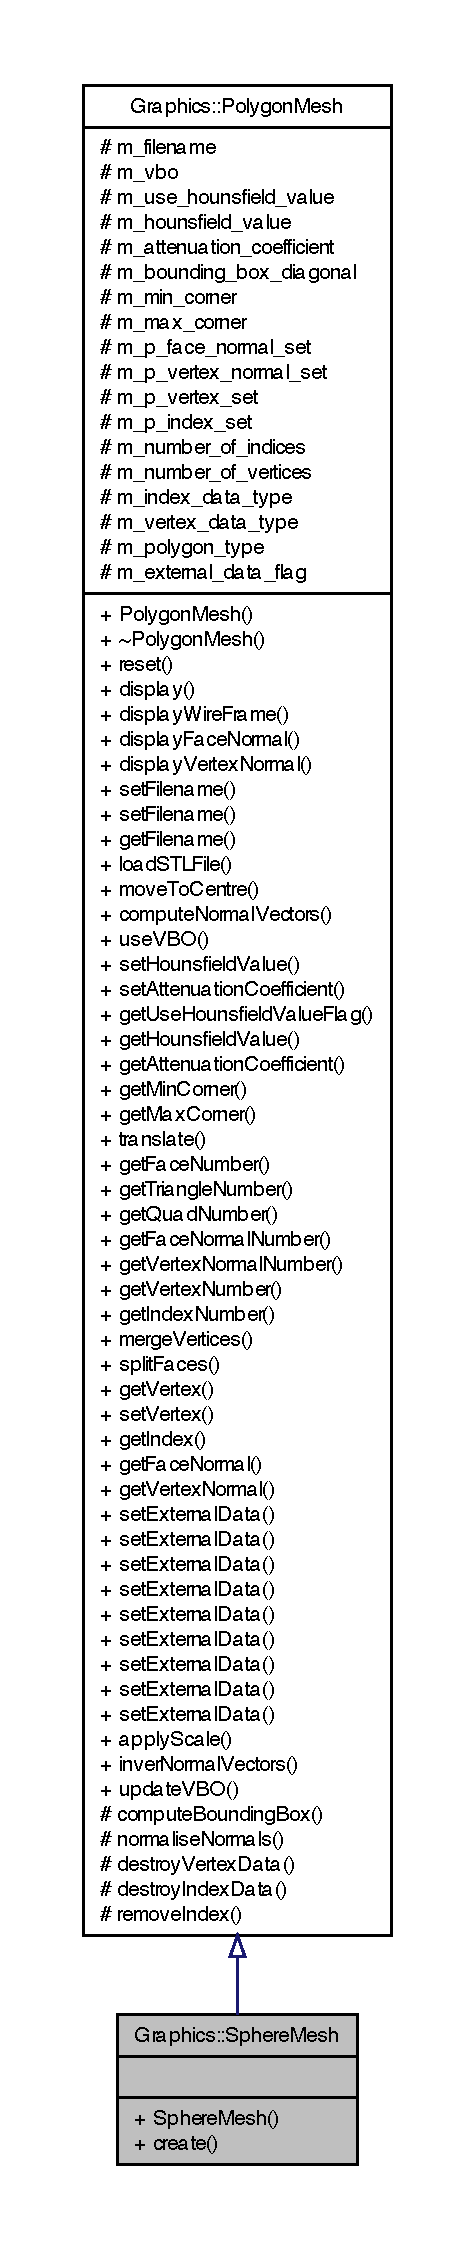
\includegraphics[height=600pt]{class_graphics_1_1_sphere_mesh__inherit__graph}
\end{center}
\end{figure}


Collaboration diagram for Graphics::SphereMesh:
\nopagebreak
\begin{figure}[H]
\begin{center}
\leavevmode
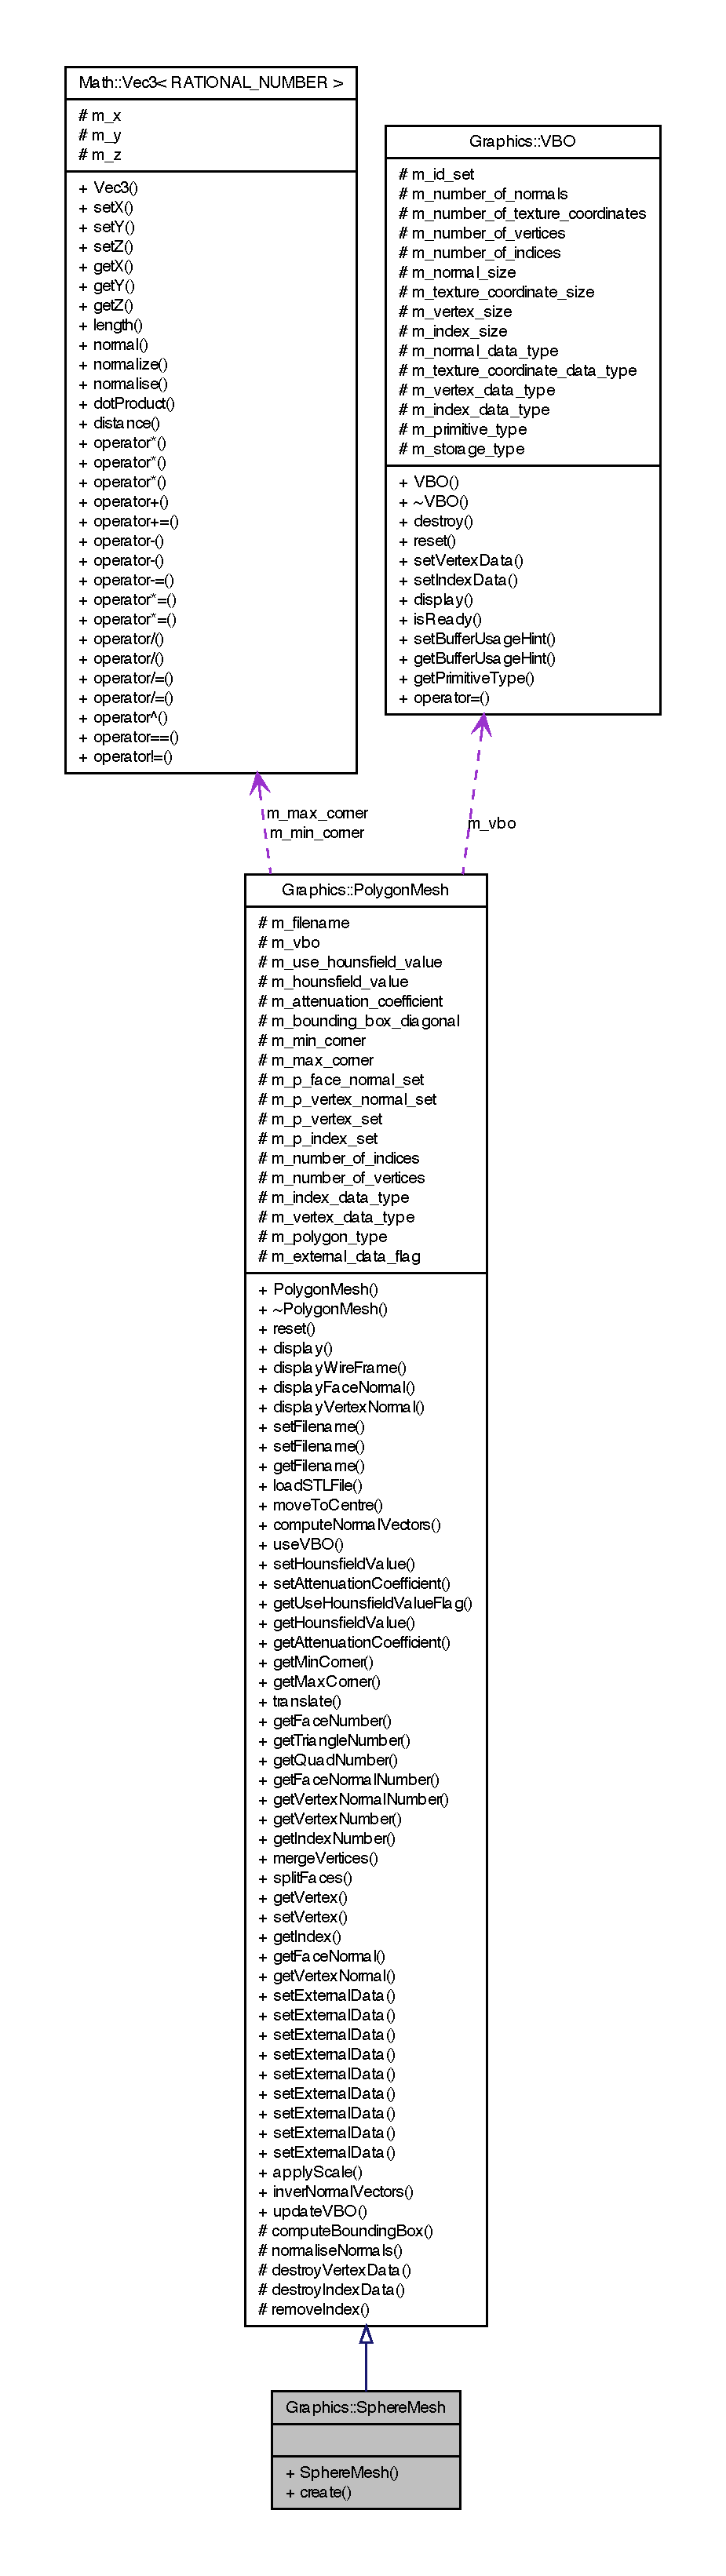
\includegraphics[height=600pt]{class_graphics_1_1_sphere_mesh__coll__graph}
\end{center}
\end{figure}
\subsection*{Public Member Functions}
\begin{DoxyCompactItemize}
\item 
\hyperlink{class_graphics_1_1_sphere_mesh_a9eb9e7ccc0805f33186c392dbc1d483c}{SphereMesh} (unsigned int aNumberOfRings=10, unsigned int aNumberOfSectors=10, float aRadius=0.5 $\ast$cm)
\begin{DoxyCompactList}\small\item\em Default constructor. \end{DoxyCompactList}\item 
void \hyperlink{class_graphics_1_1_sphere_mesh_a10cca63e76640befa47fe5aeb7665b8a}{create} (unsigned int aNumberOfRings=10, unsigned int aNumberOfSectors=10, float aRadius=0.5 $\ast$cm)
\begin{DoxyCompactList}\small\item\em Create a new sphere. \end{DoxyCompactList}\end{DoxyCompactItemize}


\subsection{Detailed Description}
\hyperlink{class_graphics_1_1_sphere_mesh}{SphereMesh} is a class to handle 3D meshes of spheres. 

Definition at line 63 of file SphereMesh.h.



\subsection{Constructor \& Destructor Documentation}
\hypertarget{class_graphics_1_1_sphere_mesh_a9eb9e7ccc0805f33186c392dbc1d483c}{
\index{Graphics::SphereMesh@{Graphics::SphereMesh}!SphereMesh@{SphereMesh}}
\index{SphereMesh@{SphereMesh}!Graphics::SphereMesh@{Graphics::SphereMesh}}
\subsubsection[{SphereMesh}]{\setlength{\rightskip}{0pt plus 5cm}Graphics::SphereMesh::SphereMesh (
\begin{DoxyParamCaption}
\item[{unsigned int}]{aNumberOfRings = {\ttfamily 10}, }
\item[{unsigned int}]{aNumberOfSectors = {\ttfamily 10}, }
\item[{float}]{aRadius = {\ttfamily 0.5~$\ast$~cm}}
\end{DoxyParamCaption}
)\hspace{0.3cm}{\ttfamily  \mbox{[}inline\mbox{]}}}}
\label{class_graphics_1_1_sphere_mesh_a9eb9e7ccc0805f33186c392dbc1d483c}


Default constructor. 



Definition at line 54 of file SphereMesh.inl.



\subsection{Member Function Documentation}
\hypertarget{class_graphics_1_1_sphere_mesh_a10cca63e76640befa47fe5aeb7665b8a}{
\index{Graphics::SphereMesh@{Graphics::SphereMesh}!create@{create}}
\index{create@{create}!Graphics::SphereMesh@{Graphics::SphereMesh}}
\subsubsection[{create}]{\setlength{\rightskip}{0pt plus 5cm}void Graphics::SphereMesh::create (
\begin{DoxyParamCaption}
\item[{unsigned int}]{aNumberOfRings = {\ttfamily 10}, }
\item[{unsigned int}]{aNumberOfSectors = {\ttfamily 10}, }
\item[{float}]{aRadius = {\ttfamily 0.5~$\ast$cm}}
\end{DoxyParamCaption}
)}}
\label{class_graphics_1_1_sphere_mesh_a10cca63e76640befa47fe5aeb7665b8a}


Create a new sphere. 



The documentation for this class was generated from the following files:\begin{DoxyCompactItemize}
\item 
/Users/fpvidal/Documents/gvirtualxray-\/code/trunk/include/gVirtualXRay/\hyperlink{_sphere_mesh_8h}{SphereMesh.h}\item 
/Users/fpvidal/Documents/gvirtualxray-\/code/trunk/include/gVirtualXRay/\hyperlink{_sphere_mesh_8inl}{SphereMesh.inl}\end{DoxyCompactItemize}

\hypertarget{class_graphics_1_1_stereo_helper}{
\section{Graphics::StereoHelper Class Reference}
\label{class_graphics_1_1_stereo_helper}\index{Graphics::StereoHelper@{Graphics::StereoHelper}}
}


\hyperlink{class_graphics_1_1_stereo_helper}{StereoHelper} is a class to handle stereo vision using OpenGL's quad buffer.  




{\ttfamily \#include $<$StereoHelper.h$>$}



Collaboration diagram for Graphics::StereoHelper:\nopagebreak
\begin{figure}[H]
\begin{center}
\leavevmode
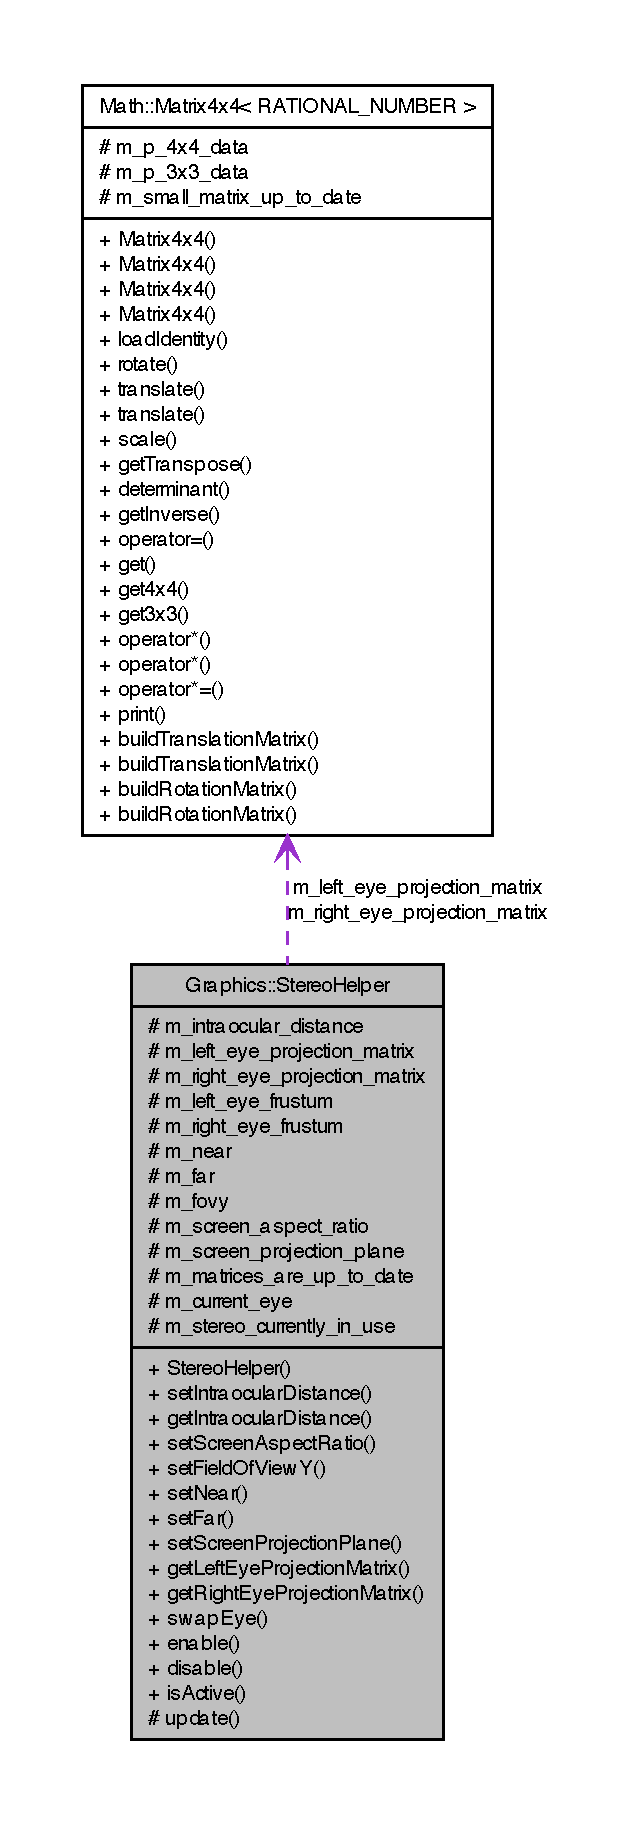
\includegraphics[height=600pt]{class_graphics_1_1_stereo_helper__coll__graph}
\end{center}
\end{figure}
\subsection*{Public Types}
\begin{DoxyCompactItemize}
\item 
enum \hyperlink{class_graphics_1_1_stereo_helper_a3878d00d8c9d23837a978e28f2602917}{EyeTypeTag} \{ \hyperlink{class_graphics_1_1_stereo_helper_a3878d00d8c9d23837a978e28f2602917a0b0e634652bf644fd9740646d8368b73}{LEFT\_\-EYE} =  0, 
\hyperlink{class_graphics_1_1_stereo_helper_a3878d00d8c9d23837a978e28f2602917ac3a76f087475575ac46057d4ad720886}{RIGHT\_\-EYE} =  1, 
\hyperlink{class_graphics_1_1_stereo_helper_a3878d00d8c9d23837a978e28f2602917aad680115cb2c639ff5955e22084de77b}{MONO} =  2
 \}
\begin{DoxyCompactList}\small\item\em Enum defining eyes. \end{DoxyCompactList}\item 
typedef enum \hyperlink{class_graphics_1_1_stereo_helper_a3878d00d8c9d23837a978e28f2602917}{Graphics::StereoHelper::EyeTypeTag} \hyperlink{class_graphics_1_1_stereo_helper_a29cdc9bdc1c46342adb6e0b06d6ee49a}{EyeType}
\begin{DoxyCompactList}\small\item\em Enum defining eyes. \end{DoxyCompactList}\end{DoxyCompactItemize}
\subsection*{Public Member Functions}
\begin{DoxyCompactItemize}
\item 
\hyperlink{class_graphics_1_1_stereo_helper_a4d75cf7dd224b52ea3b04d9b3f454ea5}{StereoHelper} ()
\begin{DoxyCompactList}\small\item\em Default constructor. \end{DoxyCompactList}\item 
void \hyperlink{class_graphics_1_1_stereo_helper_a618e05eb0080aba955bbbeea19956d32}{setIntraocularDistance} (double aDistance)
\begin{DoxyCompactList}\small\item\em Set the intraocular distance. \end{DoxyCompactList}\item 
double \hyperlink{class_graphics_1_1_stereo_helper_ae5b7d42db1fb2bd3123ded6e7afe1df6}{getIntraocularDistance} () const 
\begin{DoxyCompactList}\small\item\em Accessor on the intraocular distance. \end{DoxyCompactList}\item 
void \hyperlink{class_graphics_1_1_stereo_helper_a0a56378ca52792d45c3e2030fcdff313}{setScreenAspectRatio} (double aRatio)
\begin{DoxyCompactList}\small\item\em Set the screen aspect ratio. \end{DoxyCompactList}\item 
void \hyperlink{class_graphics_1_1_stereo_helper_ac46befc03c787da9275084cf7afed778}{setFieldOfViewY} (double aFOVY)
\begin{DoxyCompactList}\small\item\em Set the field of view along the y-\/axis. \end{DoxyCompactList}\item 
void \hyperlink{class_graphics_1_1_stereo_helper_aa67798ee18abb482b9fdd047e662c1ab}{setNear} (double aPlane)
\begin{DoxyCompactList}\small\item\em Set the near clipping plane. \end{DoxyCompactList}\item 
void \hyperlink{class_graphics_1_1_stereo_helper_a3e495bcd6b6d17d590973a732b9ed761}{setFar} (double aPlane)
\begin{DoxyCompactList}\small\item\em Set the far clipping plane. \end{DoxyCompactList}\item 
void \hyperlink{class_graphics_1_1_stereo_helper_a219235f12aa3391406fe63cd5576e0b6}{setScreenProjectionPlane} (double aPlane)
\begin{DoxyCompactList}\small\item\em Set the screen projection plane. \end{DoxyCompactList}\item 
const \hyperlink{class_math_1_1_matrix4x4}{MATRIX4} \& \hyperlink{class_graphics_1_1_stereo_helper_a83b299d08edc918b625f24389344518d}{getLeftEyeProjectionMatrix} ()
\begin{DoxyCompactList}\small\item\em Accessor on the projection matrix corresponding to the left eye. \end{DoxyCompactList}\item 
const \hyperlink{class_math_1_1_matrix4x4}{MATRIX4} \& \hyperlink{class_graphics_1_1_stereo_helper_a3f099ee2d19cf7dd794cdc52297b7e34}{getRightEyeProjectionMatrix} ()
\begin{DoxyCompactList}\small\item\em Accessor on the projection matrix corresponding to the right eye. \end{DoxyCompactList}\item 
void \hyperlink{class_graphics_1_1_stereo_helper_a3fd807eb117ce72ef569c2e5fb1dbfbe}{swapEye} ()
\begin{DoxyCompactList}\small\item\em Swap eye. \end{DoxyCompactList}\item 
bool \hyperlink{class_graphics_1_1_stereo_helper_ac4d54917c650bb098dd0247d1ec058fa}{enable} ()
\begin{DoxyCompactList}\small\item\em Enable the stereo if possible. \end{DoxyCompactList}\item 
void \hyperlink{class_graphics_1_1_stereo_helper_a64356f4ad22021f35ed9e0078adbd543}{disable} ()
\begin{DoxyCompactList}\small\item\em Disable the stereo. \end{DoxyCompactList}\item 
bool \hyperlink{class_graphics_1_1_stereo_helper_a1a822c8ed8db21db0805ab1ab622c6c2}{isActive} () const 
\begin{DoxyCompactList}\small\item\em Accessor on the stereo flag. \end{DoxyCompactList}\end{DoxyCompactItemize}
\subsection*{Protected Member Functions}
\begin{DoxyCompactItemize}
\item 
void \hyperlink{class_graphics_1_1_stereo_helper_ab355550a23d88f275eed384e3304a2df}{update} ()
\begin{DoxyCompactList}\small\item\em Compute the projection matrices. \end{DoxyCompactList}\end{DoxyCompactItemize}
\subsection*{Protected Attributes}
\begin{DoxyCompactItemize}
\item 
double \hyperlink{class_graphics_1_1_stereo_helper_a13736b824aee087d5a8bc948f8bc700d}{m\_\-intraocular\_\-distance}
\begin{DoxyCompactList}\small\item\em Intraocular distance. \end{DoxyCompactList}\item 
\hyperlink{class_math_1_1_matrix4x4}{MATRIX4} \hyperlink{class_graphics_1_1_stereo_helper_abe0f5805dd94b0d277b00c7d8ce89fd1}{m\_\-left\_\-eye\_\-projection\_\-matrix}
\begin{DoxyCompactList}\small\item\em The projection matrix corresponding to the left eye. \end{DoxyCompactList}\item 
\hyperlink{class_math_1_1_matrix4x4}{MATRIX4} \hyperlink{class_graphics_1_1_stereo_helper_aaf3d810febcca0e5c47bcc1924e8b576}{m\_\-right\_\-eye\_\-projection\_\-matrix}
\begin{DoxyCompactList}\small\item\em The projection matrix corresponding to the right eye. \end{DoxyCompactList}\item 
double \hyperlink{class_graphics_1_1_stereo_helper_a912a430f01899bb0e2ebeec941dc6801}{m\_\-left\_\-eye\_\-frustum} \mbox{[}4\mbox{]}
\item 
double \hyperlink{class_graphics_1_1_stereo_helper_a2542b4e8d37d72b4bb0ed2e7c3bc919f}{m\_\-right\_\-eye\_\-frustum} \mbox{[}4\mbox{]}
\item 
double \hyperlink{class_graphics_1_1_stereo_helper_ab6261035a7d4ed8d7de0a56a53efcaae}{m\_\-near}
\begin{DoxyCompactList}\small\item\em Near clipping plane. \end{DoxyCompactList}\item 
double \hyperlink{class_graphics_1_1_stereo_helper_adaf953e95e951648a78c1be3af5a7245}{m\_\-far}
\begin{DoxyCompactList}\small\item\em Far clipping plane. \end{DoxyCompactList}\item 
double \hyperlink{class_graphics_1_1_stereo_helper_a21f4b593c9629fe91c8f4aa3fdc3fde7}{m\_\-fovy}
\begin{DoxyCompactList}\small\item\em Field of view along the y-\/axis. \end{DoxyCompactList}\item 
double \hyperlink{class_graphics_1_1_stereo_helper_add543d27ae84db5cbcb664c7c7c08e3b}{m\_\-screen\_\-aspect\_\-ratio}
\begin{DoxyCompactList}\small\item\em Screen aspect ratio. \end{DoxyCompactList}\item 
double \hyperlink{class_graphics_1_1_stereo_helper_a0049a88c84fd0b377b69f6cb7cd4ab86}{m\_\-screen\_\-projection\_\-plane}
\begin{DoxyCompactList}\small\item\em Screen projection plane. \end{DoxyCompactList}\item 
bool \hyperlink{class_graphics_1_1_stereo_helper_a83274d674fe2f833ecab9dc67a32c64d}{m\_\-matrices\_\-are\_\-up\_\-to\_\-date}
\begin{DoxyCompactList}\small\item\em Flag set to true when the matrices are up-\/to-\/date. \end{DoxyCompactList}\item 
\hyperlink{class_graphics_1_1_stereo_helper_a29cdc9bdc1c46342adb6e0b06d6ee49a}{EyeType} \hyperlink{class_graphics_1_1_stereo_helper_aa32df0fd8c66f7fb8e3922f6413bb421}{m\_\-current\_\-eye}
\begin{DoxyCompactList}\small\item\em Current eye type. \end{DoxyCompactList}\item 
bool \hyperlink{class_graphics_1_1_stereo_helper_a01fb4aa644375cbdeb6fe98aa2c42452}{m\_\-stereo\_\-currently\_\-in\_\-use}
\begin{DoxyCompactList}\small\item\em Flag set to true when the stereo is in used. \end{DoxyCompactList}\end{DoxyCompactItemize}


\subsection{Detailed Description}
\hyperlink{class_graphics_1_1_stereo_helper}{StereoHelper} is a class to handle stereo vision using OpenGL's quad buffer. 

Definition at line 60 of file StereoHelper.h.



\subsection{Member Typedef Documentation}
\hypertarget{class_graphics_1_1_stereo_helper_a29cdc9bdc1c46342adb6e0b06d6ee49a}{
\index{Graphics::StereoHelper@{Graphics::StereoHelper}!EyeType@{EyeType}}
\index{EyeType@{EyeType}!Graphics::StereoHelper@{Graphics::StereoHelper}}
\subsubsection[{EyeType}]{\setlength{\rightskip}{0pt plus 5cm}typedef enum {\bf Graphics::StereoHelper::EyeTypeTag}  {\bf Graphics::StereoHelper::EyeType}}}
\label{class_graphics_1_1_stereo_helper_a29cdc9bdc1c46342adb6e0b06d6ee49a}


Enum defining eyes. 



\subsection{Member Enumeration Documentation}
\hypertarget{class_graphics_1_1_stereo_helper_a3878d00d8c9d23837a978e28f2602917}{
\index{Graphics::StereoHelper@{Graphics::StereoHelper}!EyeTypeTag@{EyeTypeTag}}
\index{EyeTypeTag@{EyeTypeTag}!Graphics::StereoHelper@{Graphics::StereoHelper}}
\subsubsection[{EyeTypeTag}]{\setlength{\rightskip}{0pt plus 5cm}enum {\bf Graphics::StereoHelper::EyeTypeTag}}}
\label{class_graphics_1_1_stereo_helper_a3878d00d8c9d23837a978e28f2602917}


Enum defining eyes. 

\begin{Desc}
\item[Enumerator: ]\par
\begin{description}
\index{LEFT\_\-EYE@{LEFT\_\-EYE}!Graphics::StereoHelper@{Graphics::StereoHelper}}\index{Graphics::StereoHelper@{Graphics::StereoHelper}!LEFT\_\-EYE@{LEFT\_\-EYE}}\item[{\em 
\hypertarget{class_graphics_1_1_stereo_helper_a3878d00d8c9d23837a978e28f2602917a0b0e634652bf644fd9740646d8368b73}{
LEFT\_\-EYE}
\label{class_graphics_1_1_stereo_helper_a3878d00d8c9d23837a978e28f2602917a0b0e634652bf644fd9740646d8368b73}
}]\index{RIGHT\_\-EYE@{RIGHT\_\-EYE}!Graphics::StereoHelper@{Graphics::StereoHelper}}\index{Graphics::StereoHelper@{Graphics::StereoHelper}!RIGHT\_\-EYE@{RIGHT\_\-EYE}}\item[{\em 
\hypertarget{class_graphics_1_1_stereo_helper_a3878d00d8c9d23837a978e28f2602917ac3a76f087475575ac46057d4ad720886}{
RIGHT\_\-EYE}
\label{class_graphics_1_1_stereo_helper_a3878d00d8c9d23837a978e28f2602917ac3a76f087475575ac46057d4ad720886}
}]\index{MONO@{MONO}!Graphics::StereoHelper@{Graphics::StereoHelper}}\index{Graphics::StereoHelper@{Graphics::StereoHelper}!MONO@{MONO}}\item[{\em 
\hypertarget{class_graphics_1_1_stereo_helper_a3878d00d8c9d23837a978e28f2602917aad680115cb2c639ff5955e22084de77b}{
MONO}
\label{class_graphics_1_1_stereo_helper_a3878d00d8c9d23837a978e28f2602917aad680115cb2c639ff5955e22084de77b}
}]\end{description}
\end{Desc}



Definition at line 68 of file StereoHelper.h.



\subsection{Constructor \& Destructor Documentation}
\hypertarget{class_graphics_1_1_stereo_helper_a4d75cf7dd224b52ea3b04d9b3f454ea5}{
\index{Graphics::StereoHelper@{Graphics::StereoHelper}!StereoHelper@{StereoHelper}}
\index{StereoHelper@{StereoHelper}!Graphics::StereoHelper@{Graphics::StereoHelper}}
\subsubsection[{StereoHelper}]{\setlength{\rightskip}{0pt plus 5cm}Graphics::StereoHelper::StereoHelper (
\begin{DoxyParamCaption}
{}
\end{DoxyParamCaption}
)}}
\label{class_graphics_1_1_stereo_helper_a4d75cf7dd224b52ea3b04d9b3f454ea5}


Default constructor. 



\subsection{Member Function Documentation}
\hypertarget{class_graphics_1_1_stereo_helper_a64356f4ad22021f35ed9e0078adbd543}{
\index{Graphics::StereoHelper@{Graphics::StereoHelper}!disable@{disable}}
\index{disable@{disable}!Graphics::StereoHelper@{Graphics::StereoHelper}}
\subsubsection[{disable}]{\setlength{\rightskip}{0pt plus 5cm}void Graphics::StereoHelper::disable (
\begin{DoxyParamCaption}
{}
\end{DoxyParamCaption}
)}}
\label{class_graphics_1_1_stereo_helper_a64356f4ad22021f35ed9e0078adbd543}


Disable the stereo. 

\hypertarget{class_graphics_1_1_stereo_helper_ac4d54917c650bb098dd0247d1ec058fa}{
\index{Graphics::StereoHelper@{Graphics::StereoHelper}!enable@{enable}}
\index{enable@{enable}!Graphics::StereoHelper@{Graphics::StereoHelper}}
\subsubsection[{enable}]{\setlength{\rightskip}{0pt plus 5cm}bool Graphics::StereoHelper::enable (
\begin{DoxyParamCaption}
{}
\end{DoxyParamCaption}
)}}
\label{class_graphics_1_1_stereo_helper_ac4d54917c650bb098dd0247d1ec058fa}


Enable the stereo if possible. 

\hypertarget{class_graphics_1_1_stereo_helper_ae5b7d42db1fb2bd3123ded6e7afe1df6}{
\index{Graphics::StereoHelper@{Graphics::StereoHelper}!getIntraocularDistance@{getIntraocularDistance}}
\index{getIntraocularDistance@{getIntraocularDistance}!Graphics::StereoHelper@{Graphics::StereoHelper}}
\subsubsection[{getIntraocularDistance}]{\setlength{\rightskip}{0pt plus 5cm}double Graphics::StereoHelper::getIntraocularDistance (
\begin{DoxyParamCaption}
{}
\end{DoxyParamCaption}
) const\hspace{0.3cm}{\ttfamily  \mbox{[}inline\mbox{]}}}}
\label{class_graphics_1_1_stereo_helper_ae5b7d42db1fb2bd3123ded6e7afe1df6}


Accessor on the intraocular distance. 

\begin{DoxyReturn}{Returns}
the intraocular distance 
\end{DoxyReturn}


Definition at line 47 of file StereoHelper.inl.

\hypertarget{class_graphics_1_1_stereo_helper_a83b299d08edc918b625f24389344518d}{
\index{Graphics::StereoHelper@{Graphics::StereoHelper}!getLeftEyeProjectionMatrix@{getLeftEyeProjectionMatrix}}
\index{getLeftEyeProjectionMatrix@{getLeftEyeProjectionMatrix}!Graphics::StereoHelper@{Graphics::StereoHelper}}
\subsubsection[{getLeftEyeProjectionMatrix}]{\setlength{\rightskip}{0pt plus 5cm}const {\bf MATRIX4} \& Graphics::StereoHelper::getLeftEyeProjectionMatrix (
\begin{DoxyParamCaption}
{}
\end{DoxyParamCaption}
)\hspace{0.3cm}{\ttfamily  \mbox{[}inline\mbox{]}}}}
\label{class_graphics_1_1_stereo_helper_a83b299d08edc918b625f24389344518d}


Accessor on the projection matrix corresponding to the left eye. 

\begin{DoxyReturn}{Returns}
the projection matrix 
\end{DoxyReturn}


Definition at line 100 of file StereoHelper.inl.

\hypertarget{class_graphics_1_1_stereo_helper_a3f099ee2d19cf7dd794cdc52297b7e34}{
\index{Graphics::StereoHelper@{Graphics::StereoHelper}!getRightEyeProjectionMatrix@{getRightEyeProjectionMatrix}}
\index{getRightEyeProjectionMatrix@{getRightEyeProjectionMatrix}!Graphics::StereoHelper@{Graphics::StereoHelper}}
\subsubsection[{getRightEyeProjectionMatrix}]{\setlength{\rightskip}{0pt plus 5cm}const {\bf MATRIX4} \& Graphics::StereoHelper::getRightEyeProjectionMatrix (
\begin{DoxyParamCaption}
{}
\end{DoxyParamCaption}
)\hspace{0.3cm}{\ttfamily  \mbox{[}inline\mbox{]}}}}
\label{class_graphics_1_1_stereo_helper_a3f099ee2d19cf7dd794cdc52297b7e34}


Accessor on the projection matrix corresponding to the right eye. 

\begin{DoxyReturn}{Returns}
the projection matrix 
\end{DoxyReturn}


Definition at line 113 of file StereoHelper.inl.

\hypertarget{class_graphics_1_1_stereo_helper_a1a822c8ed8db21db0805ab1ab622c6c2}{
\index{Graphics::StereoHelper@{Graphics::StereoHelper}!isActive@{isActive}}
\index{isActive@{isActive}!Graphics::StereoHelper@{Graphics::StereoHelper}}
\subsubsection[{isActive}]{\setlength{\rightskip}{0pt plus 5cm}bool Graphics::StereoHelper::isActive (
\begin{DoxyParamCaption}
{}
\end{DoxyParamCaption}
) const\hspace{0.3cm}{\ttfamily  \mbox{[}inline\mbox{]}}}}
\label{class_graphics_1_1_stereo_helper_a1a822c8ed8db21db0805ab1ab622c6c2}


Accessor on the stereo flag. 



Definition at line 126 of file StereoHelper.inl.

\hypertarget{class_graphics_1_1_stereo_helper_a3e495bcd6b6d17d590973a732b9ed761}{
\index{Graphics::StereoHelper@{Graphics::StereoHelper}!setFar@{setFar}}
\index{setFar@{setFar}!Graphics::StereoHelper@{Graphics::StereoHelper}}
\subsubsection[{setFar}]{\setlength{\rightskip}{0pt plus 5cm}void Graphics::StereoHelper::setFar (
\begin{DoxyParamCaption}
\item[{double}]{aPlane}
\end{DoxyParamCaption}
)\hspace{0.3cm}{\ttfamily  \mbox{[}inline\mbox{]}}}}
\label{class_graphics_1_1_stereo_helper_a3e495bcd6b6d17d590973a732b9ed761}


Set the far clipping plane. 


\begin{DoxyParams}{Parameters}
{\em aPlane,:} & the far clipping plane \\
\hline
\end{DoxyParams}


Definition at line 82 of file StereoHelper.inl.

\hypertarget{class_graphics_1_1_stereo_helper_ac46befc03c787da9275084cf7afed778}{
\index{Graphics::StereoHelper@{Graphics::StereoHelper}!setFieldOfViewY@{setFieldOfViewY}}
\index{setFieldOfViewY@{setFieldOfViewY}!Graphics::StereoHelper@{Graphics::StereoHelper}}
\subsubsection[{setFieldOfViewY}]{\setlength{\rightskip}{0pt plus 5cm}void Graphics::StereoHelper::setFieldOfViewY (
\begin{DoxyParamCaption}
\item[{double}]{aFOVY}
\end{DoxyParamCaption}
)\hspace{0.3cm}{\ttfamily  \mbox{[}inline\mbox{]}}}}
\label{class_graphics_1_1_stereo_helper_ac46befc03c787da9275084cf7afed778}


Set the field of view along the y-\/axis. 


\begin{DoxyParams}{Parameters}
{\em aFOVY,:} & the field of view along the y-\/axis \\
\hline
\end{DoxyParams}


Definition at line 64 of file StereoHelper.inl.

\hypertarget{class_graphics_1_1_stereo_helper_a618e05eb0080aba955bbbeea19956d32}{
\index{Graphics::StereoHelper@{Graphics::StereoHelper}!setIntraocularDistance@{setIntraocularDistance}}
\index{setIntraocularDistance@{setIntraocularDistance}!Graphics::StereoHelper@{Graphics::StereoHelper}}
\subsubsection[{setIntraocularDistance}]{\setlength{\rightskip}{0pt plus 5cm}void Graphics::StereoHelper::setIntraocularDistance (
\begin{DoxyParamCaption}
\item[{double}]{aDistance}
\end{DoxyParamCaption}
)\hspace{0.3cm}{\ttfamily  \mbox{[}inline\mbox{]}}}}
\label{class_graphics_1_1_stereo_helper_a618e05eb0080aba955bbbeea19956d32}


Set the intraocular distance. 


\begin{DoxyParams}{Parameters}
{\em aDistance,:} & the intraocular distance \\
\hline
\end{DoxyParams}


Definition at line 38 of file StereoHelper.inl.

\hypertarget{class_graphics_1_1_stereo_helper_aa67798ee18abb482b9fdd047e662c1ab}{
\index{Graphics::StereoHelper@{Graphics::StereoHelper}!setNear@{setNear}}
\index{setNear@{setNear}!Graphics::StereoHelper@{Graphics::StereoHelper}}
\subsubsection[{setNear}]{\setlength{\rightskip}{0pt plus 5cm}void Graphics::StereoHelper::setNear (
\begin{DoxyParamCaption}
\item[{double}]{aPlane}
\end{DoxyParamCaption}
)\hspace{0.3cm}{\ttfamily  \mbox{[}inline\mbox{]}}}}
\label{class_graphics_1_1_stereo_helper_aa67798ee18abb482b9fdd047e662c1ab}


Set the near clipping plane. 


\begin{DoxyParams}{Parameters}
{\em aPlane,:} & the near clipping plane \\
\hline
\end{DoxyParams}


Definition at line 73 of file StereoHelper.inl.

\hypertarget{class_graphics_1_1_stereo_helper_a0a56378ca52792d45c3e2030fcdff313}{
\index{Graphics::StereoHelper@{Graphics::StereoHelper}!setScreenAspectRatio@{setScreenAspectRatio}}
\index{setScreenAspectRatio@{setScreenAspectRatio}!Graphics::StereoHelper@{Graphics::StereoHelper}}
\subsubsection[{setScreenAspectRatio}]{\setlength{\rightskip}{0pt plus 5cm}void Graphics::StereoHelper::setScreenAspectRatio (
\begin{DoxyParamCaption}
\item[{double}]{aRatio}
\end{DoxyParamCaption}
)\hspace{0.3cm}{\ttfamily  \mbox{[}inline\mbox{]}}}}
\label{class_graphics_1_1_stereo_helper_a0a56378ca52792d45c3e2030fcdff313}


Set the screen aspect ratio. 


\begin{DoxyParams}{Parameters}
{\em aRatio,:} & the screen aspect ratio \\
\hline
\end{DoxyParams}


Definition at line 55 of file StereoHelper.inl.

\hypertarget{class_graphics_1_1_stereo_helper_a219235f12aa3391406fe63cd5576e0b6}{
\index{Graphics::StereoHelper@{Graphics::StereoHelper}!setScreenProjectionPlane@{setScreenProjectionPlane}}
\index{setScreenProjectionPlane@{setScreenProjectionPlane}!Graphics::StereoHelper@{Graphics::StereoHelper}}
\subsubsection[{setScreenProjectionPlane}]{\setlength{\rightskip}{0pt plus 5cm}void Graphics::StereoHelper::setScreenProjectionPlane (
\begin{DoxyParamCaption}
\item[{double}]{aPlane}
\end{DoxyParamCaption}
)\hspace{0.3cm}{\ttfamily  \mbox{[}inline\mbox{]}}}}
\label{class_graphics_1_1_stereo_helper_a219235f12aa3391406fe63cd5576e0b6}


Set the screen projection plane. 


\begin{DoxyParams}{Parameters}
{\em aPlane,:} & the screen projection plane \\
\hline
\end{DoxyParams}


Definition at line 91 of file StereoHelper.inl.

\hypertarget{class_graphics_1_1_stereo_helper_a3fd807eb117ce72ef569c2e5fb1dbfbe}{
\index{Graphics::StereoHelper@{Graphics::StereoHelper}!swapEye@{swapEye}}
\index{swapEye@{swapEye}!Graphics::StereoHelper@{Graphics::StereoHelper}}
\subsubsection[{swapEye}]{\setlength{\rightskip}{0pt plus 5cm}void Graphics::StereoHelper::swapEye (
\begin{DoxyParamCaption}
{}
\end{DoxyParamCaption}
)}}
\label{class_graphics_1_1_stereo_helper_a3fd807eb117ce72ef569c2e5fb1dbfbe}


Swap eye. 

\hypertarget{class_graphics_1_1_stereo_helper_ab355550a23d88f275eed384e3304a2df}{
\index{Graphics::StereoHelper@{Graphics::StereoHelper}!update@{update}}
\index{update@{update}!Graphics::StereoHelper@{Graphics::StereoHelper}}
\subsubsection[{update}]{\setlength{\rightskip}{0pt plus 5cm}void Graphics::StereoHelper::update (
\begin{DoxyParamCaption}
{}
\end{DoxyParamCaption}
)\hspace{0.3cm}{\ttfamily  \mbox{[}protected\mbox{]}}}}
\label{class_graphics_1_1_stereo_helper_ab355550a23d88f275eed384e3304a2df}


Compute the projection matrices. 



\subsection{Member Data Documentation}
\hypertarget{class_graphics_1_1_stereo_helper_aa32df0fd8c66f7fb8e3922f6413bb421}{
\index{Graphics::StereoHelper@{Graphics::StereoHelper}!m\_\-current\_\-eye@{m\_\-current\_\-eye}}
\index{m\_\-current\_\-eye@{m\_\-current\_\-eye}!Graphics::StereoHelper@{Graphics::StereoHelper}}
\subsubsection[{m\_\-current\_\-eye}]{\setlength{\rightskip}{0pt plus 5cm}{\bf EyeType} {\bf Graphics::StereoHelper::m\_\-current\_\-eye}\hspace{0.3cm}{\ttfamily  \mbox{[}protected\mbox{]}}}}
\label{class_graphics_1_1_stereo_helper_aa32df0fd8c66f7fb8e3922f6413bb421}


Current eye type. 



Definition at line 246 of file StereoHelper.h.

\hypertarget{class_graphics_1_1_stereo_helper_adaf953e95e951648a78c1be3af5a7245}{
\index{Graphics::StereoHelper@{Graphics::StereoHelper}!m\_\-far@{m\_\-far}}
\index{m\_\-far@{m\_\-far}!Graphics::StereoHelper@{Graphics::StereoHelper}}
\subsubsection[{m\_\-far}]{\setlength{\rightskip}{0pt plus 5cm}double {\bf Graphics::StereoHelper::m\_\-far}\hspace{0.3cm}{\ttfamily  \mbox{[}protected\mbox{]}}}}
\label{class_graphics_1_1_stereo_helper_adaf953e95e951648a78c1be3af5a7245}


Far clipping plane. 



Definition at line 226 of file StereoHelper.h.

\hypertarget{class_graphics_1_1_stereo_helper_a21f4b593c9629fe91c8f4aa3fdc3fde7}{
\index{Graphics::StereoHelper@{Graphics::StereoHelper}!m\_\-fovy@{m\_\-fovy}}
\index{m\_\-fovy@{m\_\-fovy}!Graphics::StereoHelper@{Graphics::StereoHelper}}
\subsubsection[{m\_\-fovy}]{\setlength{\rightskip}{0pt plus 5cm}double {\bf Graphics::StereoHelper::m\_\-fovy}\hspace{0.3cm}{\ttfamily  \mbox{[}protected\mbox{]}}}}
\label{class_graphics_1_1_stereo_helper_a21f4b593c9629fe91c8f4aa3fdc3fde7}


Field of view along the y-\/axis. 



Definition at line 230 of file StereoHelper.h.

\hypertarget{class_graphics_1_1_stereo_helper_a13736b824aee087d5a8bc948f8bc700d}{
\index{Graphics::StereoHelper@{Graphics::StereoHelper}!m\_\-intraocular\_\-distance@{m\_\-intraocular\_\-distance}}
\index{m\_\-intraocular\_\-distance@{m\_\-intraocular\_\-distance}!Graphics::StereoHelper@{Graphics::StereoHelper}}
\subsubsection[{m\_\-intraocular\_\-distance}]{\setlength{\rightskip}{0pt plus 5cm}double {\bf Graphics::StereoHelper::m\_\-intraocular\_\-distance}\hspace{0.3cm}{\ttfamily  \mbox{[}protected\mbox{]}}}}
\label{class_graphics_1_1_stereo_helper_a13736b824aee087d5a8bc948f8bc700d}


Intraocular distance. 



Definition at line 194 of file StereoHelper.h.

\hypertarget{class_graphics_1_1_stereo_helper_a912a430f01899bb0e2ebeec941dc6801}{
\index{Graphics::StereoHelper@{Graphics::StereoHelper}!m\_\-left\_\-eye\_\-frustum@{m\_\-left\_\-eye\_\-frustum}}
\index{m\_\-left\_\-eye\_\-frustum@{m\_\-left\_\-eye\_\-frustum}!Graphics::StereoHelper@{Graphics::StereoHelper}}
\subsubsection[{m\_\-left\_\-eye\_\-frustum}]{\setlength{\rightskip}{0pt plus 5cm}double {\bf Graphics::StereoHelper::m\_\-left\_\-eye\_\-frustum}\mbox{[}4\mbox{]}\hspace{0.3cm}{\ttfamily  \mbox{[}protected\mbox{]}}}}
\label{class_graphics_1_1_stereo_helper_a912a430f01899bb0e2ebeec941dc6801}
Frustum of the left eye m\_\-left\_\-eye\_\-frustum\mbox{[}0\mbox{]} corresponds to the left clipping plane m\_\-left\_\-eye\_\-frustum\mbox{[}1\mbox{]} corresponds to the right clipping plane m\_\-left\_\-eye\_\-frustum\mbox{[}2\mbox{]} corresponds to the bottom clipping plane m\_\-left\_\-eye\_\-frustum\mbox{[}3\mbox{]} corresponds to the top clipping plane 

Definition at line 210 of file StereoHelper.h.

\hypertarget{class_graphics_1_1_stereo_helper_abe0f5805dd94b0d277b00c7d8ce89fd1}{
\index{Graphics::StereoHelper@{Graphics::StereoHelper}!m\_\-left\_\-eye\_\-projection\_\-matrix@{m\_\-left\_\-eye\_\-projection\_\-matrix}}
\index{m\_\-left\_\-eye\_\-projection\_\-matrix@{m\_\-left\_\-eye\_\-projection\_\-matrix}!Graphics::StereoHelper@{Graphics::StereoHelper}}
\subsubsection[{m\_\-left\_\-eye\_\-projection\_\-matrix}]{\setlength{\rightskip}{0pt plus 5cm}{\bf MATRIX4} {\bf Graphics::StereoHelper::m\_\-left\_\-eye\_\-projection\_\-matrix}\hspace{0.3cm}{\ttfamily  \mbox{[}protected\mbox{]}}}}
\label{class_graphics_1_1_stereo_helper_abe0f5805dd94b0d277b00c7d8ce89fd1}


The projection matrix corresponding to the left eye. 



Definition at line 198 of file StereoHelper.h.

\hypertarget{class_graphics_1_1_stereo_helper_a83274d674fe2f833ecab9dc67a32c64d}{
\index{Graphics::StereoHelper@{Graphics::StereoHelper}!m\_\-matrices\_\-are\_\-up\_\-to\_\-date@{m\_\-matrices\_\-are\_\-up\_\-to\_\-date}}
\index{m\_\-matrices\_\-are\_\-up\_\-to\_\-date@{m\_\-matrices\_\-are\_\-up\_\-to\_\-date}!Graphics::StereoHelper@{Graphics::StereoHelper}}
\subsubsection[{m\_\-matrices\_\-are\_\-up\_\-to\_\-date}]{\setlength{\rightskip}{0pt plus 5cm}bool {\bf Graphics::StereoHelper::m\_\-matrices\_\-are\_\-up\_\-to\_\-date}\hspace{0.3cm}{\ttfamily  \mbox{[}protected\mbox{]}}}}
\label{class_graphics_1_1_stereo_helper_a83274d674fe2f833ecab9dc67a32c64d}


Flag set to true when the matrices are up-\/to-\/date. 



Definition at line 242 of file StereoHelper.h.

\hypertarget{class_graphics_1_1_stereo_helper_ab6261035a7d4ed8d7de0a56a53efcaae}{
\index{Graphics::StereoHelper@{Graphics::StereoHelper}!m\_\-near@{m\_\-near}}
\index{m\_\-near@{m\_\-near}!Graphics::StereoHelper@{Graphics::StereoHelper}}
\subsubsection[{m\_\-near}]{\setlength{\rightskip}{0pt plus 5cm}double {\bf Graphics::StereoHelper::m\_\-near}\hspace{0.3cm}{\ttfamily  \mbox{[}protected\mbox{]}}}}
\label{class_graphics_1_1_stereo_helper_ab6261035a7d4ed8d7de0a56a53efcaae}


Near clipping plane. 



Definition at line 222 of file StereoHelper.h.

\hypertarget{class_graphics_1_1_stereo_helper_a2542b4e8d37d72b4bb0ed2e7c3bc919f}{
\index{Graphics::StereoHelper@{Graphics::StereoHelper}!m\_\-right\_\-eye\_\-frustum@{m\_\-right\_\-eye\_\-frustum}}
\index{m\_\-right\_\-eye\_\-frustum@{m\_\-right\_\-eye\_\-frustum}!Graphics::StereoHelper@{Graphics::StereoHelper}}
\subsubsection[{m\_\-right\_\-eye\_\-frustum}]{\setlength{\rightskip}{0pt plus 5cm}double {\bf Graphics::StereoHelper::m\_\-right\_\-eye\_\-frustum}\mbox{[}4\mbox{]}\hspace{0.3cm}{\ttfamily  \mbox{[}protected\mbox{]}}}}
\label{class_graphics_1_1_stereo_helper_a2542b4e8d37d72b4bb0ed2e7c3bc919f}
Frustum of the right eye m\_\-right\_\-eye\_\-frustum\mbox{[}0\mbox{]} corresponds to the left clipping plane m\_\-right\_\-eye\_\-frustum\mbox{[}1\mbox{]} corresponds to the right clipping plane m\_\-right\_\-eye\_\-frustum\mbox{[}2\mbox{]} corresponds to the bottom clipping plane m\_\-right\_\-eye\_\-frustum\mbox{[}3\mbox{]} corresponds to the top clipping plane 

Definition at line 218 of file StereoHelper.h.

\hypertarget{class_graphics_1_1_stereo_helper_aaf3d810febcca0e5c47bcc1924e8b576}{
\index{Graphics::StereoHelper@{Graphics::StereoHelper}!m\_\-right\_\-eye\_\-projection\_\-matrix@{m\_\-right\_\-eye\_\-projection\_\-matrix}}
\index{m\_\-right\_\-eye\_\-projection\_\-matrix@{m\_\-right\_\-eye\_\-projection\_\-matrix}!Graphics::StereoHelper@{Graphics::StereoHelper}}
\subsubsection[{m\_\-right\_\-eye\_\-projection\_\-matrix}]{\setlength{\rightskip}{0pt plus 5cm}{\bf MATRIX4} {\bf Graphics::StereoHelper::m\_\-right\_\-eye\_\-projection\_\-matrix}\hspace{0.3cm}{\ttfamily  \mbox{[}protected\mbox{]}}}}
\label{class_graphics_1_1_stereo_helper_aaf3d810febcca0e5c47bcc1924e8b576}


The projection matrix corresponding to the right eye. 



Definition at line 202 of file StereoHelper.h.

\hypertarget{class_graphics_1_1_stereo_helper_add543d27ae84db5cbcb664c7c7c08e3b}{
\index{Graphics::StereoHelper@{Graphics::StereoHelper}!m\_\-screen\_\-aspect\_\-ratio@{m\_\-screen\_\-aspect\_\-ratio}}
\index{m\_\-screen\_\-aspect\_\-ratio@{m\_\-screen\_\-aspect\_\-ratio}!Graphics::StereoHelper@{Graphics::StereoHelper}}
\subsubsection[{m\_\-screen\_\-aspect\_\-ratio}]{\setlength{\rightskip}{0pt plus 5cm}double {\bf Graphics::StereoHelper::m\_\-screen\_\-aspect\_\-ratio}\hspace{0.3cm}{\ttfamily  \mbox{[}protected\mbox{]}}}}
\label{class_graphics_1_1_stereo_helper_add543d27ae84db5cbcb664c7c7c08e3b}


Screen aspect ratio. 



Definition at line 234 of file StereoHelper.h.

\hypertarget{class_graphics_1_1_stereo_helper_a0049a88c84fd0b377b69f6cb7cd4ab86}{
\index{Graphics::StereoHelper@{Graphics::StereoHelper}!m\_\-screen\_\-projection\_\-plane@{m\_\-screen\_\-projection\_\-plane}}
\index{m\_\-screen\_\-projection\_\-plane@{m\_\-screen\_\-projection\_\-plane}!Graphics::StereoHelper@{Graphics::StereoHelper}}
\subsubsection[{m\_\-screen\_\-projection\_\-plane}]{\setlength{\rightskip}{0pt plus 5cm}double {\bf Graphics::StereoHelper::m\_\-screen\_\-projection\_\-plane}\hspace{0.3cm}{\ttfamily  \mbox{[}protected\mbox{]}}}}
\label{class_graphics_1_1_stereo_helper_a0049a88c84fd0b377b69f6cb7cd4ab86}


Screen projection plane. 



Definition at line 238 of file StereoHelper.h.

\hypertarget{class_graphics_1_1_stereo_helper_a01fb4aa644375cbdeb6fe98aa2c42452}{
\index{Graphics::StereoHelper@{Graphics::StereoHelper}!m\_\-stereo\_\-currently\_\-in\_\-use@{m\_\-stereo\_\-currently\_\-in\_\-use}}
\index{m\_\-stereo\_\-currently\_\-in\_\-use@{m\_\-stereo\_\-currently\_\-in\_\-use}!Graphics::StereoHelper@{Graphics::StereoHelper}}
\subsubsection[{m\_\-stereo\_\-currently\_\-in\_\-use}]{\setlength{\rightskip}{0pt plus 5cm}bool {\bf Graphics::StereoHelper::m\_\-stereo\_\-currently\_\-in\_\-use}\hspace{0.3cm}{\ttfamily  \mbox{[}protected\mbox{]}}}}
\label{class_graphics_1_1_stereo_helper_a01fb4aa644375cbdeb6fe98aa2c42452}


Flag set to true when the stereo is in used. 



Definition at line 250 of file StereoHelper.h.



The documentation for this class was generated from the following files:\begin{DoxyCompactItemize}
\item 
/Users/fpvidal/Documents/gvirtualxray-\/code/trunk/include/gVirtualXRay/\hyperlink{_stereo_helper_8h}{StereoHelper.h}\item 
/Users/fpvidal/Documents/gvirtualxray-\/code/trunk/include/gVirtualXRay/\hyperlink{_stereo_helper_8inl}{StereoHelper.inl}\end{DoxyCompactItemize}

\hypertarget{class_graphics_1_1_v_b_o}{
\section{Graphics::VBO Class Reference}
\label{class_graphics_1_1_v_b_o}\index{Graphics::VBO@{Graphics::VBO}}
}


\hyperlink{class_graphics_1_1_v_b_o}{VBO} is a class to handle a vertex buffer object (\hyperlink{class_graphics_1_1_v_b_o}{VBO}).  




{\ttfamily \#include $<$VBO.h$>$}

\subsection*{Public Member Functions}
\begin{DoxyCompactItemize}
\item 
\hyperlink{class_graphics_1_1_v_b_o_a5fdd4892ea05b7d9609270183247feb1}{VBO} ()
\begin{DoxyCompactList}\small\item\em Default constructor. \end{DoxyCompactList}\item 
\hyperlink{class_graphics_1_1_v_b_o_a0f393478113752bf9baa4324497cdf63}{$\sim$VBO} ()
\begin{DoxyCompactList}\small\item\em Destructor. \end{DoxyCompactList}\item 
void \hyperlink{class_graphics_1_1_v_b_o_ae5b7f5a0ba9e52a80691d3239ed7ca76}{destroy} ()
\begin{DoxyCompactList}\small\item\em Release the data on the GPU. \end{DoxyCompactList}\item 
void \hyperlink{class_graphics_1_1_v_b_o_a499016a22e57972350cb4d79fb2fc683}{reset} ()
\begin{DoxyCompactList}\small\item\em Reset the data. \end{DoxyCompactList}\item 
void \hyperlink{class_graphics_1_1_v_b_o_a904d82132f6bc0151adbbfef15664b58}{setVertexData} (int aPrimitiveType, const unsigned int aNumberOfVertices, unsigned int aNumberOfCompontentsPerVertex, int aVertexDataType, const void $\ast$apVertices, const unsigned int aNumberOfNormals, unsigned int aNumberOfCompontentsPerNormal, int aNormalDataType, const void $\ast$apNormals, const unsigned int aNumberOfTextureCoordinates, unsigned int aNumberOfCompontentsPerCoord, int aCoordDataType, const void $\ast$apTextureCoordinates)
\begin{DoxyCompactList}\small\item\em Set the vertex data. \end{DoxyCompactList}\item 
void \hyperlink{class_graphics_1_1_v_b_o_ad898dedd6cfc1323666d0c92362b0cb6}{setIndexData} (const unsigned int aNumberOfIndexes, int anIndexDataType, const void $\ast$apIndexSet)
\begin{DoxyCompactList}\small\item\em Set the index. \end{DoxyCompactList}\item 
void \hyperlink{class_graphics_1_1_v_b_o_a317d5e66f907a1c4ce1c62fd13027e94}{display} () const 
\begin{DoxyCompactList}\small\item\em Display the triangular mesh using OpenGL. \end{DoxyCompactList}\item 
bool \hyperlink{class_graphics_1_1_v_b_o_a1d0a57f5c94120de14f5f7fc146a7e02}{isReady} () const 
\begin{DoxyCompactList}\small\item\em Check if the vertex buffer object is ready. \end{DoxyCompactList}\item 
void \hyperlink{class_graphics_1_1_v_b_o_ae62f61a5171472bbc4a4b009b8ab197c}{setBufferUsageHint} (int aFlag)
\item 
int \hyperlink{class_graphics_1_1_v_b_o_acb61a094b658fee807d4964cfbec3211}{getBufferUsageHint} () const 
\begin{DoxyCompactList}\small\item\em Accessor on the buffer usage hint. \end{DoxyCompactList}\item 
int \hyperlink{class_graphics_1_1_v_b_o_a3ae4a9302e98c599f2a7688c1417d083}{getPrimitiveType} () const 
\begin{DoxyCompactList}\small\item\em Accessor on the primitive type. \end{DoxyCompactList}\item 
\hyperlink{class_graphics_1_1_v_b_o}{VBO} \& \hyperlink{class_graphics_1_1_v_b_o_a9d3f17037047f1febb746cc0bdf65280}{operator=} (const \hyperlink{class_graphics_1_1_v_b_o}{VBO} \&aVbo)
\begin{DoxyCompactList}\small\item\em Copy operator. \end{DoxyCompactList}\end{DoxyCompactItemize}
\subsection*{Protected Attributes}
\begin{DoxyCompactItemize}
\item 
unsigned int \hyperlink{class_graphics_1_1_v_b_o_a2070c3221265c092f68f8c970f225ddb}{m\_\-id\_\-set} \mbox{[}4\mbox{]}
\begin{DoxyCompactList}\small\item\em ID of VBOs. \end{DoxyCompactList}\item 
unsigned int \hyperlink{class_graphics_1_1_v_b_o_a1c096f3f5c8df8c7688450b70cb0e6cd}{m\_\-number\_\-of\_\-normals}
\begin{DoxyCompactList}\small\item\em Number of normal vectors. \end{DoxyCompactList}\item 
unsigned int \hyperlink{class_graphics_1_1_v_b_o_a085a9d24e4c8b1278730362ea34504e5}{m\_\-number\_\-of\_\-texture\_\-coordinates}
\begin{DoxyCompactList}\small\item\em Number of vertices. \end{DoxyCompactList}\item 
unsigned int \hyperlink{class_graphics_1_1_v_b_o_ac9ab09212702f66a1941cbd83dc109a6}{m\_\-number\_\-of\_\-vertices}
\begin{DoxyCompactList}\small\item\em Number of vertices. \end{DoxyCompactList}\item 
unsigned int \hyperlink{class_graphics_1_1_v_b_o_a251b1299ea9eb738c398b0f0f61264c7}{m\_\-number\_\-of\_\-indices}
\begin{DoxyCompactList}\small\item\em Number of indices. \end{DoxyCompactList}\item 
unsigned int \hyperlink{class_graphics_1_1_v_b_o_a57b327ff027f5565d207a6c0d1127f9c}{m\_\-normal\_\-size}
\begin{DoxyCompactList}\small\item\em Size in bytes of the array of normal vectors. \end{DoxyCompactList}\item 
unsigned int \hyperlink{class_graphics_1_1_v_b_o_ad764a9816e96edc1ed1659bcd64e9796}{m\_\-texture\_\-coordinate\_\-size}
\begin{DoxyCompactList}\small\item\em Size in bytes of the array of texture coordinates. \end{DoxyCompactList}\item 
unsigned int \hyperlink{class_graphics_1_1_v_b_o_a22a4fa87cd40138f131e8dc3e604053c}{m\_\-vertex\_\-size}
\begin{DoxyCompactList}\small\item\em Size in bytes of the array of vertices. \end{DoxyCompactList}\item 
unsigned int \hyperlink{class_graphics_1_1_v_b_o_a6aee1be4b03097c901914f138cfb70d2}{m\_\-index\_\-size}
\begin{DoxyCompactList}\small\item\em Size in bytes of the array of indices. \end{DoxyCompactList}\item 
int \hyperlink{class_graphics_1_1_v_b_o_acc73a624adcb5819c83fdee509032dc8}{m\_\-normal\_\-data\_\-type}
\begin{DoxyCompactList}\small\item\em Data type of normal vectors; valid values are GL\_\-FLOAT and GL\_\-DOUBLE. \end{DoxyCompactList}\item 
int \hyperlink{class_graphics_1_1_v_b_o_a450479bb177f1b603baab9e809f8a3fe}{m\_\-texture\_\-coordinate\_\-data\_\-type}
\begin{DoxyCompactList}\small\item\em Data type of texture coordinates; valid values are GL\_\-FLOAT and GL\_\-DOUBLE. \end{DoxyCompactList}\item 
int \hyperlink{class_graphics_1_1_v_b_o_a5c41a622ac8a3b1a2798d8fa69d53db6}{m\_\-vertex\_\-data\_\-type}
\begin{DoxyCompactList}\small\item\em Data type of vertices; valid values are GL\_\-FLOAT and GL\_\-DOUBLE. \end{DoxyCompactList}\item 
int \hyperlink{class_graphics_1_1_v_b_o_a87e3330b9c688d6981c1b23fcfeab9a5}{m\_\-index\_\-data\_\-type}
\begin{DoxyCompactList}\small\item\em Data type of indices; valid values are GL\_\-UNSIGNED\_\-BYTE, GL\_\-UNSIGNED\_\-SHORT and GL\_\-UNSIGNED\_\-INT. \end{DoxyCompactList}\item 
int \hyperlink{class_graphics_1_1_v_b_o_ac19f07fa0f8258b35782d3feee846316}{m\_\-primitive\_\-type}
\begin{DoxyCompactList}\small\item\em Type of primitive to draw; valid values are GL\_\-POINTS, GL\_\-LINE\_\-STRIP, GL\_\-LINE\_\-LOOP, GL\_\-LINES, GL\_\-LINE\_\-STRIP\_\-ADJACENCY, GL\_\-LINES\_\-ADJACENCY, GL\_\-TRIANGLE\_\-STRIP, GL\_\-TRIANGLE\_\-FAN, GL\_\-TRIANGLES, GL\_\-TRIANGLE\_\-STRIP\_\-ADJACENCY, GL\_\-TRIANGLES\_\-ADJACENCY and GL\_\-PATCHES. \end{DoxyCompactList}\item 
int \hyperlink{class_graphics_1_1_v_b_o_a5f534f57456b712463a2c7cf7cf4f249}{m\_\-storage\_\-type}
\begin{DoxyCompactList}\small\item\em The buffer usage hint; valid values are GL\_\-DYNAMIC\_\-DRAW, GL\_\-STATIC\_\-DRAW and GL\_\-STREAM\_\-DRAW. \end{DoxyCompactList}\end{DoxyCompactItemize}


\subsection{Detailed Description}
\hyperlink{class_graphics_1_1_v_b_o}{VBO} is a class to handle a vertex buffer object (\hyperlink{class_graphics_1_1_v_b_o}{VBO}). 

Definition at line 45 of file VBO.h.



\subsection{Constructor \& Destructor Documentation}
\hypertarget{class_graphics_1_1_v_b_o_a5fdd4892ea05b7d9609270183247feb1}{
\index{Graphics::VBO@{Graphics::VBO}!VBO@{VBO}}
\index{VBO@{VBO}!Graphics::VBO@{Graphics::VBO}}
\subsubsection[{VBO}]{\setlength{\rightskip}{0pt plus 5cm}Graphics::VBO::VBO (
\begin{DoxyParamCaption}
{}
\end{DoxyParamCaption}
)}}
\label{class_graphics_1_1_v_b_o_a5fdd4892ea05b7d9609270183247feb1}


Default constructor. 

\hypertarget{class_graphics_1_1_v_b_o_a0f393478113752bf9baa4324497cdf63}{
\index{Graphics::VBO@{Graphics::VBO}!$\sim$VBO@{$\sim$VBO}}
\index{$\sim$VBO@{$\sim$VBO}!Graphics::VBO@{Graphics::VBO}}
\subsubsection[{$\sim$VBO}]{\setlength{\rightskip}{0pt plus 5cm}Graphics::VBO::$\sim$VBO (
\begin{DoxyParamCaption}
{}
\end{DoxyParamCaption}
)\hspace{0.3cm}{\ttfamily  \mbox{[}inline\mbox{]}}}}
\label{class_graphics_1_1_v_b_o_a0f393478113752bf9baa4324497cdf63}


Destructor. 



Definition at line 59 of file VBO.inl.



\subsection{Member Function Documentation}
\hypertarget{class_graphics_1_1_v_b_o_ae5b7f5a0ba9e52a80691d3239ed7ca76}{
\index{Graphics::VBO@{Graphics::VBO}!destroy@{destroy}}
\index{destroy@{destroy}!Graphics::VBO@{Graphics::VBO}}
\subsubsection[{destroy}]{\setlength{\rightskip}{0pt plus 5cm}void Graphics::VBO::destroy (
\begin{DoxyParamCaption}
{}
\end{DoxyParamCaption}
)}}
\label{class_graphics_1_1_v_b_o_ae5b7f5a0ba9e52a80691d3239ed7ca76}


Release the data on the GPU. 

\hypertarget{class_graphics_1_1_v_b_o_a317d5e66f907a1c4ce1c62fd13027e94}{
\index{Graphics::VBO@{Graphics::VBO}!display@{display}}
\index{display@{display}!Graphics::VBO@{Graphics::VBO}}
\subsubsection[{display}]{\setlength{\rightskip}{0pt plus 5cm}void Graphics::VBO::display (
\begin{DoxyParamCaption}
{}
\end{DoxyParamCaption}
) const}}
\label{class_graphics_1_1_v_b_o_a317d5e66f907a1c4ce1c62fd13027e94}


Display the triangular mesh using OpenGL. 

\hypertarget{class_graphics_1_1_v_b_o_acb61a094b658fee807d4964cfbec3211}{
\index{Graphics::VBO@{Graphics::VBO}!getBufferUsageHint@{getBufferUsageHint}}
\index{getBufferUsageHint@{getBufferUsageHint}!Graphics::VBO@{Graphics::VBO}}
\subsubsection[{getBufferUsageHint}]{\setlength{\rightskip}{0pt plus 5cm}int Graphics::VBO::getBufferUsageHint (
\begin{DoxyParamCaption}
{}
\end{DoxyParamCaption}
) const\hspace{0.3cm}{\ttfamily  \mbox{[}inline\mbox{]}}}}
\label{class_graphics_1_1_v_b_o_acb61a094b658fee807d4964cfbec3211}


Accessor on the buffer usage hint. 

\begin{DoxyReturn}{Returns}
the buffer usage hint 
\end{DoxyReturn}


Definition at line 83 of file VBO.inl.

\hypertarget{class_graphics_1_1_v_b_o_a3ae4a9302e98c599f2a7688c1417d083}{
\index{Graphics::VBO@{Graphics::VBO}!getPrimitiveType@{getPrimitiveType}}
\index{getPrimitiveType@{getPrimitiveType}!Graphics::VBO@{Graphics::VBO}}
\subsubsection[{getPrimitiveType}]{\setlength{\rightskip}{0pt plus 5cm}int Graphics::VBO::getPrimitiveType (
\begin{DoxyParamCaption}
{}
\end{DoxyParamCaption}
) const\hspace{0.3cm}{\ttfamily  \mbox{[}inline\mbox{]}}}}
\label{class_graphics_1_1_v_b_o_a3ae4a9302e98c599f2a7688c1417d083}


Accessor on the primitive type. 

\begin{DoxyReturn}{Returns}
the primitive type 
\end{DoxyReturn}


Definition at line 91 of file VBO.inl.

\hypertarget{class_graphics_1_1_v_b_o_a1d0a57f5c94120de14f5f7fc146a7e02}{
\index{Graphics::VBO@{Graphics::VBO}!isReady@{isReady}}
\index{isReady@{isReady}!Graphics::VBO@{Graphics::VBO}}
\subsubsection[{isReady}]{\setlength{\rightskip}{0pt plus 5cm}bool Graphics::VBO::isReady (
\begin{DoxyParamCaption}
{}
\end{DoxyParamCaption}
) const\hspace{0.3cm}{\ttfamily  \mbox{[}inline\mbox{]}}}}
\label{class_graphics_1_1_v_b_o_a1d0a57f5c94120de14f5f7fc146a7e02}


Check if the vertex buffer object is ready. 

\begin{DoxyReturn}{Returns}
true if the \hyperlink{class_graphics_1_1_v_b_o}{VBO} is ready to use, false if it is not 
\end{DoxyReturn}


Definition at line 67 of file VBO.inl.

\hypertarget{class_graphics_1_1_v_b_o_a9d3f17037047f1febb746cc0bdf65280}{
\index{Graphics::VBO@{Graphics::VBO}!operator=@{operator=}}
\index{operator=@{operator=}!Graphics::VBO@{Graphics::VBO}}
\subsubsection[{operator=}]{\setlength{\rightskip}{0pt plus 5cm}{\bf VBO} \& Graphics::VBO::operator= (
\begin{DoxyParamCaption}
\item[{const {\bf VBO} \&}]{aVbo}
\end{DoxyParamCaption}
)\hspace{0.3cm}{\ttfamily  \mbox{[}inline\mbox{]}}}}
\label{class_graphics_1_1_v_b_o_a9d3f17037047f1febb746cc0bdf65280}


Copy operator. 


\begin{DoxyParams}{Parameters}
{\em aVbo,:} & \hyperlink{class_graphics_1_1_v_b_o}{VBO} to copy \\
\hline
\end{DoxyParams}
\begin{DoxyReturn}{Returns}
the new \hyperlink{class_graphics_1_1_v_b_o}{VBO} 
\end{DoxyReturn}


Definition at line 99 of file VBO.inl.

\hypertarget{class_graphics_1_1_v_b_o_a499016a22e57972350cb4d79fb2fc683}{
\index{Graphics::VBO@{Graphics::VBO}!reset@{reset}}
\index{reset@{reset}!Graphics::VBO@{Graphics::VBO}}
\subsubsection[{reset}]{\setlength{\rightskip}{0pt plus 5cm}void Graphics::VBO::reset (
\begin{DoxyParamCaption}
{}
\end{DoxyParamCaption}
)}}
\label{class_graphics_1_1_v_b_o_a499016a22e57972350cb4d79fb2fc683}


Reset the data. 

\hypertarget{class_graphics_1_1_v_b_o_ae62f61a5171472bbc4a4b009b8ab197c}{
\index{Graphics::VBO@{Graphics::VBO}!setBufferUsageHint@{setBufferUsageHint}}
\index{setBufferUsageHint@{setBufferUsageHint}!Graphics::VBO@{Graphics::VBO}}
\subsubsection[{setBufferUsageHint}]{\setlength{\rightskip}{0pt plus 5cm}void Graphics::VBO::setBufferUsageHint (
\begin{DoxyParamCaption}
\item[{int}]{aFlag}
\end{DoxyParamCaption}
)\hspace{0.3cm}{\ttfamily  \mbox{[}inline\mbox{]}}}}
\label{class_graphics_1_1_v_b_o_ae62f61a5171472bbc4a4b009b8ab197c}
Set the buffer usage hint. Accepted values are: GL\_\-STATIC\_\-DRAW is for vertex buffers that are rendered many times, and whose contents are specified once and never change. GL\_\-DYNAMIC\_\-DRAW is for vertex buffers that are rendered many times, and whose contents change during the rendering loop. GL\_\-STREAM\_\-DRAW is for vertex buffers that are rendered a small number of times and then discarded. 
\begin{DoxyParams}{Parameters}
{\em aFlag,:} & the buffer usage hint to set \\
\hline
\end{DoxyParams}


Definition at line 75 of file VBO.inl.

\hypertarget{class_graphics_1_1_v_b_o_ad898dedd6cfc1323666d0c92362b0cb6}{
\index{Graphics::VBO@{Graphics::VBO}!setIndexData@{setIndexData}}
\index{setIndexData@{setIndexData}!Graphics::VBO@{Graphics::VBO}}
\subsubsection[{setIndexData}]{\setlength{\rightskip}{0pt plus 5cm}void Graphics::VBO::setIndexData (
\begin{DoxyParamCaption}
\item[{const unsigned int}]{aNumberOfIndexes, }
\item[{int}]{anIndexDataType, }
\item[{const void $\ast$}]{apIndexSet}
\end{DoxyParamCaption}
)}}
\label{class_graphics_1_1_v_b_o_ad898dedd6cfc1323666d0c92362b0cb6}


Set the index. 


\begin{DoxyParams}{Parameters}
{\em aNumberOfIndexes,:} & number of indices \\
\hline
{\em anIndexDataType,:} & the data type of indices; valid values are GL\_\-UNSGINED\_\-BYTE, GL\_\-UNSGINED\_\-SHORT and GL\_\-UNSGINED\_\-INT \\
\hline
{\em apIndexSet,:} & the index set \\
\hline
\end{DoxyParams}
\hypertarget{class_graphics_1_1_v_b_o_a904d82132f6bc0151adbbfef15664b58}{
\index{Graphics::VBO@{Graphics::VBO}!setVertexData@{setVertexData}}
\index{setVertexData@{setVertexData}!Graphics::VBO@{Graphics::VBO}}
\subsubsection[{setVertexData}]{\setlength{\rightskip}{0pt plus 5cm}void Graphics::VBO::setVertexData (
\begin{DoxyParamCaption}
\item[{int}]{aPrimitiveType, }
\item[{const unsigned int}]{aNumberOfVertices, }
\item[{unsigned int}]{aNumberOfCompontentsPerVertex, }
\item[{int}]{aVertexDataType, }
\item[{const void $\ast$}]{apVertices, }
\item[{const unsigned int}]{aNumberOfNormals, }
\item[{unsigned int}]{aNumberOfCompontentsPerNormal, }
\item[{int}]{aNormalDataType, }
\item[{const void $\ast$}]{apNormals, }
\item[{const unsigned int}]{aNumberOfTextureCoordinates, }
\item[{unsigned int}]{aNumberOfCompontentsPerCoord, }
\item[{int}]{aCoordDataType, }
\item[{const void $\ast$}]{apTextureCoordinates}
\end{DoxyParamCaption}
)}}
\label{class_graphics_1_1_v_b_o_a904d82132f6bc0151adbbfef15664b58}


Set the vertex data. 


\begin{DoxyParams}{Parameters}
{\em aPrimitiveType,:} & the primitive type; valid values are: GL\_\-POINTS, GL\_\-LINE\_\-STRIP, GL\_\-LINE\_\-LOOP, GL\_\-LINES, GL\_\-LINE\_\-STRIP\_\-ADJACENCY, GL\_\-LINES\_\-ADJACENCY, GL\_\-TRIANGLE\_\-STRIP, GL\_\-TRIANGLE\_\-FAN, GL\_\-TRIANGLES, GL\_\-TRIANGLE\_\-STRIP\_\-ADJACENCY, GL\_\-TRIANGLES\_\-ADJACENCY and GL\_\-PATCHES \\
\hline
{\em aNumberOfVertices,:} & number of vertices \\
\hline
{\em aNumberOfCompontentsPerVertex,:} & the number of component per vertex \\
\hline
{\em aVertexDataType,:} & the data type of vertices; valid values are GL\_\-FLOAT and GL\_\-DOUBLE \\
\hline
{\em apVertices,:} & address of the first component of the first vertex \\
\hline
{\em aNumberOfNormals,:} & number of normal vectors \\
\hline
{\em aNumberOfCompontentsPerNormal,:} & the number of component per normal vector \\
\hline
{\em aNormalDataType,:} & the data type of normal vectors; valid values are GL\_\-FLOAT and GL\_\-DOUBLE \\
\hline
{\em apNormals,:} & address of the first component of the firth normal vector \\
\hline
{\em aNumberOfTextureCoordinates,:} & number of texture coordinates \\
\hline
{\em aNumberOfCompontentsPerCoord,:} & the number of component per texture coordinate \\
\hline
{\em aCoordDataType,:} & the data type of texture coordinates; valid values are GL\_\-FLOAT and GL\_\-DOUBLE \\
\hline
{\em apTextureCoordinates,:} & address of the first component of the first texture coordinate \\
\hline
\end{DoxyParams}


\subsection{Member Data Documentation}
\hypertarget{class_graphics_1_1_v_b_o_a2070c3221265c092f68f8c970f225ddb}{
\index{Graphics::VBO@{Graphics::VBO}!m\_\-id\_\-set@{m\_\-id\_\-set}}
\index{m\_\-id\_\-set@{m\_\-id\_\-set}!Graphics::VBO@{Graphics::VBO}}
\subsubsection[{m\_\-id\_\-set}]{\setlength{\rightskip}{0pt plus 5cm}unsigned int {\bf Graphics::VBO::m\_\-id\_\-set}\mbox{[}4\mbox{]}\hspace{0.3cm}{\ttfamily  \mbox{[}protected\mbox{]}}}}
\label{class_graphics_1_1_v_b_o_a2070c3221265c092f68f8c970f225ddb}


ID of VBOs. 



Definition at line 169 of file VBO.h.

\hypertarget{class_graphics_1_1_v_b_o_a87e3330b9c688d6981c1b23fcfeab9a5}{
\index{Graphics::VBO@{Graphics::VBO}!m\_\-index\_\-data\_\-type@{m\_\-index\_\-data\_\-type}}
\index{m\_\-index\_\-data\_\-type@{m\_\-index\_\-data\_\-type}!Graphics::VBO@{Graphics::VBO}}
\subsubsection[{m\_\-index\_\-data\_\-type}]{\setlength{\rightskip}{0pt plus 5cm}int {\bf Graphics::VBO::m\_\-index\_\-data\_\-type}\hspace{0.3cm}{\ttfamily  \mbox{[}protected\mbox{]}}}}
\label{class_graphics_1_1_v_b_o_a87e3330b9c688d6981c1b23fcfeab9a5}


Data type of indices; valid values are GL\_\-UNSIGNED\_\-BYTE, GL\_\-UNSIGNED\_\-SHORT and GL\_\-UNSIGNED\_\-INT. 



Definition at line 217 of file VBO.h.

\hypertarget{class_graphics_1_1_v_b_o_a6aee1be4b03097c901914f138cfb70d2}{
\index{Graphics::VBO@{Graphics::VBO}!m\_\-index\_\-size@{m\_\-index\_\-size}}
\index{m\_\-index\_\-size@{m\_\-index\_\-size}!Graphics::VBO@{Graphics::VBO}}
\subsubsection[{m\_\-index\_\-size}]{\setlength{\rightskip}{0pt plus 5cm}unsigned int {\bf Graphics::VBO::m\_\-index\_\-size}\hspace{0.3cm}{\ttfamily  \mbox{[}protected\mbox{]}}}}
\label{class_graphics_1_1_v_b_o_a6aee1be4b03097c901914f138cfb70d2}


Size in bytes of the array of indices. 



Definition at line 201 of file VBO.h.

\hypertarget{class_graphics_1_1_v_b_o_acc73a624adcb5819c83fdee509032dc8}{
\index{Graphics::VBO@{Graphics::VBO}!m\_\-normal\_\-data\_\-type@{m\_\-normal\_\-data\_\-type}}
\index{m\_\-normal\_\-data\_\-type@{m\_\-normal\_\-data\_\-type}!Graphics::VBO@{Graphics::VBO}}
\subsubsection[{m\_\-normal\_\-data\_\-type}]{\setlength{\rightskip}{0pt plus 5cm}int {\bf Graphics::VBO::m\_\-normal\_\-data\_\-type}\hspace{0.3cm}{\ttfamily  \mbox{[}protected\mbox{]}}}}
\label{class_graphics_1_1_v_b_o_acc73a624adcb5819c83fdee509032dc8}


Data type of normal vectors; valid values are GL\_\-FLOAT and GL\_\-DOUBLE. 



Definition at line 205 of file VBO.h.

\hypertarget{class_graphics_1_1_v_b_o_a57b327ff027f5565d207a6c0d1127f9c}{
\index{Graphics::VBO@{Graphics::VBO}!m\_\-normal\_\-size@{m\_\-normal\_\-size}}
\index{m\_\-normal\_\-size@{m\_\-normal\_\-size}!Graphics::VBO@{Graphics::VBO}}
\subsubsection[{m\_\-normal\_\-size}]{\setlength{\rightskip}{0pt plus 5cm}unsigned int {\bf Graphics::VBO::m\_\-normal\_\-size}\hspace{0.3cm}{\ttfamily  \mbox{[}protected\mbox{]}}}}
\label{class_graphics_1_1_v_b_o_a57b327ff027f5565d207a6c0d1127f9c}


Size in bytes of the array of normal vectors. 



Definition at line 189 of file VBO.h.

\hypertarget{class_graphics_1_1_v_b_o_a251b1299ea9eb738c398b0f0f61264c7}{
\index{Graphics::VBO@{Graphics::VBO}!m\_\-number\_\-of\_\-indices@{m\_\-number\_\-of\_\-indices}}
\index{m\_\-number\_\-of\_\-indices@{m\_\-number\_\-of\_\-indices}!Graphics::VBO@{Graphics::VBO}}
\subsubsection[{m\_\-number\_\-of\_\-indices}]{\setlength{\rightskip}{0pt plus 5cm}unsigned int {\bf Graphics::VBO::m\_\-number\_\-of\_\-indices}\hspace{0.3cm}{\ttfamily  \mbox{[}protected\mbox{]}}}}
\label{class_graphics_1_1_v_b_o_a251b1299ea9eb738c398b0f0f61264c7}


Number of indices. 



Definition at line 185 of file VBO.h.

\hypertarget{class_graphics_1_1_v_b_o_a1c096f3f5c8df8c7688450b70cb0e6cd}{
\index{Graphics::VBO@{Graphics::VBO}!m\_\-number\_\-of\_\-normals@{m\_\-number\_\-of\_\-normals}}
\index{m\_\-number\_\-of\_\-normals@{m\_\-number\_\-of\_\-normals}!Graphics::VBO@{Graphics::VBO}}
\subsubsection[{m\_\-number\_\-of\_\-normals}]{\setlength{\rightskip}{0pt plus 5cm}unsigned int {\bf Graphics::VBO::m\_\-number\_\-of\_\-normals}\hspace{0.3cm}{\ttfamily  \mbox{[}protected\mbox{]}}}}
\label{class_graphics_1_1_v_b_o_a1c096f3f5c8df8c7688450b70cb0e6cd}


Number of normal vectors. 



Definition at line 173 of file VBO.h.

\hypertarget{class_graphics_1_1_v_b_o_a085a9d24e4c8b1278730362ea34504e5}{
\index{Graphics::VBO@{Graphics::VBO}!m\_\-number\_\-of\_\-texture\_\-coordinates@{m\_\-number\_\-of\_\-texture\_\-coordinates}}
\index{m\_\-number\_\-of\_\-texture\_\-coordinates@{m\_\-number\_\-of\_\-texture\_\-coordinates}!Graphics::VBO@{Graphics::VBO}}
\subsubsection[{m\_\-number\_\-of\_\-texture\_\-coordinates}]{\setlength{\rightskip}{0pt plus 5cm}unsigned int {\bf Graphics::VBO::m\_\-number\_\-of\_\-texture\_\-coordinates}\hspace{0.3cm}{\ttfamily  \mbox{[}protected\mbox{]}}}}
\label{class_graphics_1_1_v_b_o_a085a9d24e4c8b1278730362ea34504e5}


Number of vertices. 



Definition at line 177 of file VBO.h.

\hypertarget{class_graphics_1_1_v_b_o_ac9ab09212702f66a1941cbd83dc109a6}{
\index{Graphics::VBO@{Graphics::VBO}!m\_\-number\_\-of\_\-vertices@{m\_\-number\_\-of\_\-vertices}}
\index{m\_\-number\_\-of\_\-vertices@{m\_\-number\_\-of\_\-vertices}!Graphics::VBO@{Graphics::VBO}}
\subsubsection[{m\_\-number\_\-of\_\-vertices}]{\setlength{\rightskip}{0pt plus 5cm}unsigned int {\bf Graphics::VBO::m\_\-number\_\-of\_\-vertices}\hspace{0.3cm}{\ttfamily  \mbox{[}protected\mbox{]}}}}
\label{class_graphics_1_1_v_b_o_ac9ab09212702f66a1941cbd83dc109a6}


Number of vertices. 



Definition at line 181 of file VBO.h.

\hypertarget{class_graphics_1_1_v_b_o_ac19f07fa0f8258b35782d3feee846316}{
\index{Graphics::VBO@{Graphics::VBO}!m\_\-primitive\_\-type@{m\_\-primitive\_\-type}}
\index{m\_\-primitive\_\-type@{m\_\-primitive\_\-type}!Graphics::VBO@{Graphics::VBO}}
\subsubsection[{m\_\-primitive\_\-type}]{\setlength{\rightskip}{0pt plus 5cm}int {\bf Graphics::VBO::m\_\-primitive\_\-type}\hspace{0.3cm}{\ttfamily  \mbox{[}protected\mbox{]}}}}
\label{class_graphics_1_1_v_b_o_ac19f07fa0f8258b35782d3feee846316}


Type of primitive to draw; valid values are GL\_\-POINTS, GL\_\-LINE\_\-STRIP, GL\_\-LINE\_\-LOOP, GL\_\-LINES, GL\_\-LINE\_\-STRIP\_\-ADJACENCY, GL\_\-LINES\_\-ADJACENCY, GL\_\-TRIANGLE\_\-STRIP, GL\_\-TRIANGLE\_\-FAN, GL\_\-TRIANGLES, GL\_\-TRIANGLE\_\-STRIP\_\-ADJACENCY, GL\_\-TRIANGLES\_\-ADJACENCY and GL\_\-PATCHES. 



Definition at line 221 of file VBO.h.

\hypertarget{class_graphics_1_1_v_b_o_a5f534f57456b712463a2c7cf7cf4f249}{
\index{Graphics::VBO@{Graphics::VBO}!m\_\-storage\_\-type@{m\_\-storage\_\-type}}
\index{m\_\-storage\_\-type@{m\_\-storage\_\-type}!Graphics::VBO@{Graphics::VBO}}
\subsubsection[{m\_\-storage\_\-type}]{\setlength{\rightskip}{0pt plus 5cm}int {\bf Graphics::VBO::m\_\-storage\_\-type}\hspace{0.3cm}{\ttfamily  \mbox{[}protected\mbox{]}}}}
\label{class_graphics_1_1_v_b_o_a5f534f57456b712463a2c7cf7cf4f249}


The buffer usage hint; valid values are GL\_\-DYNAMIC\_\-DRAW, GL\_\-STATIC\_\-DRAW and GL\_\-STREAM\_\-DRAW. 



Definition at line 225 of file VBO.h.

\hypertarget{class_graphics_1_1_v_b_o_a450479bb177f1b603baab9e809f8a3fe}{
\index{Graphics::VBO@{Graphics::VBO}!m\_\-texture\_\-coordinate\_\-data\_\-type@{m\_\-texture\_\-coordinate\_\-data\_\-type}}
\index{m\_\-texture\_\-coordinate\_\-data\_\-type@{m\_\-texture\_\-coordinate\_\-data\_\-type}!Graphics::VBO@{Graphics::VBO}}
\subsubsection[{m\_\-texture\_\-coordinate\_\-data\_\-type}]{\setlength{\rightskip}{0pt plus 5cm}int {\bf Graphics::VBO::m\_\-texture\_\-coordinate\_\-data\_\-type}\hspace{0.3cm}{\ttfamily  \mbox{[}protected\mbox{]}}}}
\label{class_graphics_1_1_v_b_o_a450479bb177f1b603baab9e809f8a3fe}


Data type of texture coordinates; valid values are GL\_\-FLOAT and GL\_\-DOUBLE. 



Definition at line 209 of file VBO.h.

\hypertarget{class_graphics_1_1_v_b_o_ad764a9816e96edc1ed1659bcd64e9796}{
\index{Graphics::VBO@{Graphics::VBO}!m\_\-texture\_\-coordinate\_\-size@{m\_\-texture\_\-coordinate\_\-size}}
\index{m\_\-texture\_\-coordinate\_\-size@{m\_\-texture\_\-coordinate\_\-size}!Graphics::VBO@{Graphics::VBO}}
\subsubsection[{m\_\-texture\_\-coordinate\_\-size}]{\setlength{\rightskip}{0pt plus 5cm}unsigned int {\bf Graphics::VBO::m\_\-texture\_\-coordinate\_\-size}\hspace{0.3cm}{\ttfamily  \mbox{[}protected\mbox{]}}}}
\label{class_graphics_1_1_v_b_o_ad764a9816e96edc1ed1659bcd64e9796}


Size in bytes of the array of texture coordinates. 



Definition at line 193 of file VBO.h.

\hypertarget{class_graphics_1_1_v_b_o_a5c41a622ac8a3b1a2798d8fa69d53db6}{
\index{Graphics::VBO@{Graphics::VBO}!m\_\-vertex\_\-data\_\-type@{m\_\-vertex\_\-data\_\-type}}
\index{m\_\-vertex\_\-data\_\-type@{m\_\-vertex\_\-data\_\-type}!Graphics::VBO@{Graphics::VBO}}
\subsubsection[{m\_\-vertex\_\-data\_\-type}]{\setlength{\rightskip}{0pt plus 5cm}int {\bf Graphics::VBO::m\_\-vertex\_\-data\_\-type}\hspace{0.3cm}{\ttfamily  \mbox{[}protected\mbox{]}}}}
\label{class_graphics_1_1_v_b_o_a5c41a622ac8a3b1a2798d8fa69d53db6}


Data type of vertices; valid values are GL\_\-FLOAT and GL\_\-DOUBLE. 



Definition at line 213 of file VBO.h.

\hypertarget{class_graphics_1_1_v_b_o_a22a4fa87cd40138f131e8dc3e604053c}{
\index{Graphics::VBO@{Graphics::VBO}!m\_\-vertex\_\-size@{m\_\-vertex\_\-size}}
\index{m\_\-vertex\_\-size@{m\_\-vertex\_\-size}!Graphics::VBO@{Graphics::VBO}}
\subsubsection[{m\_\-vertex\_\-size}]{\setlength{\rightskip}{0pt plus 5cm}unsigned int {\bf Graphics::VBO::m\_\-vertex\_\-size}\hspace{0.3cm}{\ttfamily  \mbox{[}protected\mbox{]}}}}
\label{class_graphics_1_1_v_b_o_a22a4fa87cd40138f131e8dc3e604053c}


Size in bytes of the array of vertices. 



Definition at line 197 of file VBO.h.



The documentation for this class was generated from the following files:\begin{DoxyCompactItemize}
\item 
/Users/fpvidal/Documents/gvirtualxray-\/code/trunk/include/gVirtualXRay/\hyperlink{_v_b_o_8h}{VBO.h}\item 
/Users/fpvidal/Documents/gvirtualxray-\/code/trunk/include/gVirtualXRay/\hyperlink{_v_b_o_8inl}{VBO.inl}\end{DoxyCompactItemize}

\hypertarget{class_math_1_1_vec2}{
\section{Math::Vec2$<$ T $>$ Class Template Reference}
\label{class_math_1_1_vec2}\index{Math::Vec2@{Math::Vec2}}
}


\hyperlink{class_math_1_1_vec2}{Vec2} is a template class to handle a 2D vector.  




{\ttfamily \#include $<$Vec2.h$>$}



Collaboration diagram for Math::Vec2$<$ T $>$:\nopagebreak
\begin{figure}[H]
\begin{center}
\leavevmode
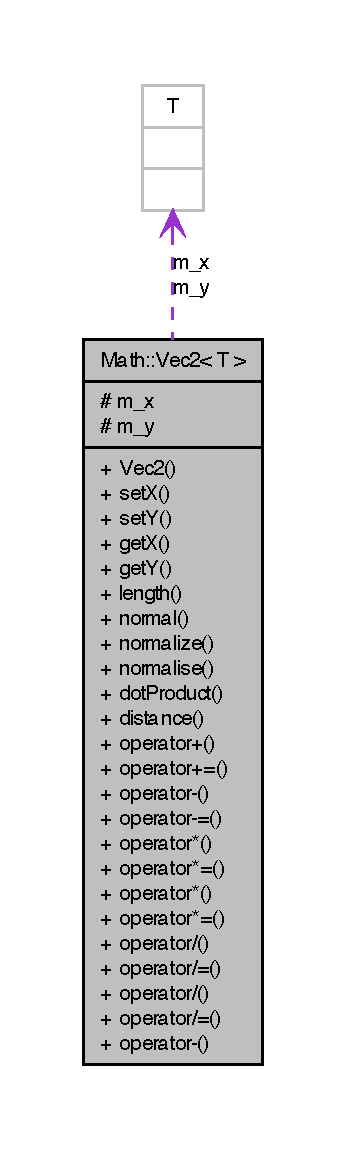
\includegraphics[width=166pt]{class_math_1_1_vec2__coll__graph}
\end{center}
\end{figure}
\subsection*{Public Member Functions}
\begin{DoxyCompactItemize}
\item 
\hyperlink{class_math_1_1_vec2_a150f8a5f9a8159902f4ec1e699c7f0e8}{Vec2} (const T \&aX=0.0f, const T \&aY=0.0f)
\begin{DoxyCompactList}\small\item\em Default Constructor. \end{DoxyCompactList}\item 
void \hyperlink{class_math_1_1_vec2_ae394c7d2d2c1330cb5fa210ec5149d0d}{setX} (const T \&aValue)
\begin{DoxyCompactList}\small\item\em Set the position along the x-\/axis. \end{DoxyCompactList}\item 
void \hyperlink{class_math_1_1_vec2_a7748fb246d30fc62d4df66644a6de50b}{setY} (const T \&aValue)
\begin{DoxyCompactList}\small\item\em Set the position along the y-\/axis. \end{DoxyCompactList}\item 
T \hyperlink{class_math_1_1_vec2_a0a655d0d8cea609614afd3915b06c48a}{getX} () const 
\begin{DoxyCompactList}\small\item\em Accessor on the position along the x-\/axis. \end{DoxyCompactList}\item 
T \hyperlink{class_math_1_1_vec2_a270be9de3e990f63e60ce5c77dfb9ce5}{getY} () const 
\begin{DoxyCompactList}\small\item\em Accessor on the position along the y-\/axis. \end{DoxyCompactList}\item 
double \hyperlink{class_math_1_1_vec2_a24a9732993bdeb320dafea6ba8acb7cb}{length} () const 
\begin{DoxyCompactList}\small\item\em Get the length of the vector. \end{DoxyCompactList}\item 
\hyperlink{class_math_1_1_vec2}{Vec2} \hyperlink{class_math_1_1_vec2_a8fc99f9aba2e1509fc87859d9ec91b5c}{normal} () const 
\begin{DoxyCompactList}\small\item\em Get the unit vector corresponding to the normed current vector. \end{DoxyCompactList}\item 
void \hyperlink{class_math_1_1_vec2_a4e0949be704200adfd16677920df5c22}{normalize} ()
\begin{DoxyCompactList}\small\item\em Normalize the current vector so that its length is 1. \end{DoxyCompactList}\item 
void \hyperlink{class_math_1_1_vec2_abab039ed4ac43257829ea970f6c3b84a}{normalise} ()
\begin{DoxyCompactList}\small\item\em Normalise the current vector so that its length is 1. \end{DoxyCompactList}\item 
double \hyperlink{class_math_1_1_vec2_aa33630fea634ace9966b11f492e7fae8}{dotProduct} (const \hyperlink{class_math_1_1_vec2}{Vec2} \&aVector) const 
\begin{DoxyCompactList}\small\item\em Get the dot product between the current vector and a given vector. \end{DoxyCompactList}\item 
double \hyperlink{class_math_1_1_vec2_af8269f91dba4f7282d280bb29a0be4dc}{distance} (const \hyperlink{class_math_1_1_vec2}{Vec2} \&aVector) const 
\item 
const \hyperlink{class_math_1_1_vec2}{Vec2} \hyperlink{class_math_1_1_vec2_a9586cbbfbdc0f921d31e7e895965133b}{operator+} (const \hyperlink{class_math_1_1_vec2}{Vec2} \&aVector) const 
\begin{DoxyCompactList}\small\item\em Operator +. \end{DoxyCompactList}\item 
\hyperlink{class_math_1_1_vec2}{Vec2} \& \hyperlink{class_math_1_1_vec2_a7e053d6826734b2a17a11daf0da4fe30}{operator+=} (const \hyperlink{class_math_1_1_vec2}{Vec2} \&aVector)
\begin{DoxyCompactList}\small\item\em Operator +=. \end{DoxyCompactList}\item 
const \hyperlink{class_math_1_1_vec2}{Vec2} \hyperlink{class_math_1_1_vec2_a38c9a2f75e8ef0b0ee54707c4a438a0a}{operator-\/} (const \hyperlink{class_math_1_1_vec2}{Vec2} \&aVector) const 
\begin{DoxyCompactList}\small\item\em Operator -\/. \end{DoxyCompactList}\item 
\hyperlink{class_math_1_1_vec2}{Vec2} \& \hyperlink{class_math_1_1_vec2_a06529205b9f170c9a03f0a56b0c17b91}{operator-\/=} (const \hyperlink{class_math_1_1_vec2}{Vec2} \&aVector)
\begin{DoxyCompactList}\small\item\em Operator -\/=. \end{DoxyCompactList}\item 
const \hyperlink{class_math_1_1_vec2}{Vec2} \hyperlink{class_math_1_1_vec2_ab5ae36da60e186bb77247905ca800bdf}{operator$\ast$} (const double \&aValue) const 
\begin{DoxyCompactList}\small\item\em Operator $\ast$ to multiply each component of the vector by a given value. \end{DoxyCompactList}\item 
\hyperlink{class_math_1_1_vec2}{Vec2} \& \hyperlink{class_math_1_1_vec2_ac4f9a930354c9ee46b949942edfe01bf}{operator$\ast$=} (const double \&aValue)
\item 
const \hyperlink{class_math_1_1_vec2}{Vec2} \hyperlink{class_math_1_1_vec2_a0f413eb407c1bc2dd12733e4f225ecfb}{operator$\ast$} (const float \&aValue) const 
\begin{DoxyCompactList}\small\item\em Operator $\ast$ to multiply each component of the vector by a given value. \end{DoxyCompactList}\item 
\hyperlink{class_math_1_1_vec2}{Vec2} \& \hyperlink{class_math_1_1_vec2_a039f22e0586253749be6a702b4a29e8b}{operator$\ast$=} (const float \&aValue)
\item 
const \hyperlink{class_math_1_1_vec2}{Vec2} \hyperlink{class_math_1_1_vec2_a813f08d209c531ab037bdf670f0f707f}{operator/} (const double \&aValue) const 
\begin{DoxyCompactList}\small\item\em Operator / to divide each component of the vector by a given value. \end{DoxyCompactList}\item 
\hyperlink{class_math_1_1_vec2}{Vec2} \& \hyperlink{class_math_1_1_vec2_aa24ccc980574f24b6b7e1adc5a44a4f4}{operator/=} (const double \&aValue)
\item 
const \hyperlink{class_math_1_1_vec2}{Vec2} \hyperlink{class_math_1_1_vec2_adfcc0849b27c2d7a16a5c8967f69c9f7}{operator/} (const float \&aValue) const 
\begin{DoxyCompactList}\small\item\em Operator / to divide each component of the vector by a given value. \end{DoxyCompactList}\item 
\hyperlink{class_math_1_1_vec2}{Vec2} \& \hyperlink{class_math_1_1_vec2_a38a63f1fc919b86e31b71b1abf2f13da}{operator/=} (const float \&aValue)
\item 
const \hyperlink{class_math_1_1_vec2}{Vec2} \hyperlink{class_math_1_1_vec2_a8a23d813b8a85704647f1a2ff63ca362}{operator-\/} () const 
\begin{DoxyCompactList}\small\item\em Operator -\/ to get the opposite vector. \end{DoxyCompactList}\end{DoxyCompactItemize}
\subsection*{Protected Attributes}
\begin{DoxyCompactItemize}
\item 
T \hyperlink{class_math_1_1_vec2_ae7e5f6fb13e2a5ef8e0e7aa5a373f18c}{m\_\-x}
\begin{DoxyCompactList}\small\item\em the position along the x-\/axis \end{DoxyCompactList}\item 
T \hyperlink{class_math_1_1_vec2_abd88545de9b57b06d6ebbdffa4824913}{m\_\-y}
\begin{DoxyCompactList}\small\item\em the position along the y-\/axi \end{DoxyCompactList}\end{DoxyCompactItemize}


\subsection{Detailed Description}
\subsubsection*{template$<$typename T$>$class Math::Vec2$<$ T $>$}

\hyperlink{class_math_1_1_vec2}{Vec2} is a template class to handle a 2D vector. 

Definition at line 58 of file Vec2.h.



\subsection{Constructor \& Destructor Documentation}
\hypertarget{class_math_1_1_vec2_a150f8a5f9a8159902f4ec1e699c7f0e8}{
\index{Math::Vec2@{Math::Vec2}!Vec2@{Vec2}}
\index{Vec2@{Vec2}!Math::Vec2@{Math::Vec2}}
\subsubsection[{Vec2}]{\setlength{\rightskip}{0pt plus 5cm}template$<$typename T$>$ {\bf Math::Vec2}$<$ T $>$::{\bf Vec2} (
\begin{DoxyParamCaption}
\item[{const T \&}]{aX = {\ttfamily 0.0f}, }
\item[{const T \&}]{aY = {\ttfamily 0.0f}}
\end{DoxyParamCaption}
)}}
\label{class_math_1_1_vec2_a150f8a5f9a8159902f4ec1e699c7f0e8}


Default Constructor. 


\begin{DoxyParams}{Parameters}
{\em aX,:} & the position along the x-\/axis \\
\hline
{\em aY,:} & the position along the y-\/axis \\
\hline
\end{DoxyParams}


Definition at line 36 of file Vec2.inl.



\subsection{Member Function Documentation}
\hypertarget{class_math_1_1_vec2_af8269f91dba4f7282d280bb29a0be4dc}{
\index{Math::Vec2@{Math::Vec2}!distance@{distance}}
\index{distance@{distance}!Math::Vec2@{Math::Vec2}}
\subsubsection[{distance}]{\setlength{\rightskip}{0pt plus 5cm}template$<$typename T $>$ double {\bf Math::Vec2}$<$ T $>$::distance (
\begin{DoxyParamCaption}
\item[{const {\bf Vec2}$<$ T $>$ \&}]{aVector}
\end{DoxyParamCaption}
) const}}
\label{class_math_1_1_vec2_af8269f91dba4f7282d280bb29a0be4dc}
Get the distance between the 2D position represented by the current vector and another position. 
\begin{DoxyParams}{Parameters}
{\em aVector,:} & the other vector \\
\hline
\end{DoxyParams}
\begin{DoxyReturn}{Returns}
the distance 
\end{DoxyReturn}


Definition at line 119 of file Vec2.inl.

\hypertarget{class_math_1_1_vec2_aa33630fea634ace9966b11f492e7fae8}{
\index{Math::Vec2@{Math::Vec2}!dotProduct@{dotProduct}}
\index{dotProduct@{dotProduct}!Math::Vec2@{Math::Vec2}}
\subsubsection[{dotProduct}]{\setlength{\rightskip}{0pt plus 5cm}template$<$typename T $>$ double {\bf Math::Vec2}$<$ T $>$::dotProduct (
\begin{DoxyParamCaption}
\item[{const {\bf Vec2}$<$ T $>$ \&}]{aVector}
\end{DoxyParamCaption}
) const}}
\label{class_math_1_1_vec2_aa33630fea634ace9966b11f492e7fae8}


Get the dot product between the current vector and a given vector. 


\begin{DoxyParams}{Parameters}
{\em aVector,:} & the other vector \\
\hline
\end{DoxyParams}
\begin{DoxyReturn}{Returns}
the dot product 
\end{DoxyReturn}


Definition at line 111 of file Vec2.inl.

\hypertarget{class_math_1_1_vec2_a0a655d0d8cea609614afd3915b06c48a}{
\index{Math::Vec2@{Math::Vec2}!getX@{getX}}
\index{getX@{getX}!Math::Vec2@{Math::Vec2}}
\subsubsection[{getX}]{\setlength{\rightskip}{0pt plus 5cm}template$<$typename T $>$ T {\bf Math::Vec2}$<$ T $>$::getX (
\begin{DoxyParamCaption}
{}
\end{DoxyParamCaption}
) const}}
\label{class_math_1_1_vec2_a0a655d0d8cea609614afd3915b06c48a}


Accessor on the position along the x-\/axis. 

\begin{DoxyReturn}{Returns}
the position along the x-\/axis 
\end{DoxyReturn}


Definition at line 61 of file Vec2.inl.

\hypertarget{class_math_1_1_vec2_a270be9de3e990f63e60ce5c77dfb9ce5}{
\index{Math::Vec2@{Math::Vec2}!getY@{getY}}
\index{getY@{getY}!Math::Vec2@{Math::Vec2}}
\subsubsection[{getY}]{\setlength{\rightskip}{0pt plus 5cm}template$<$typename T $>$ T {\bf Math::Vec2}$<$ T $>$::getY (
\begin{DoxyParamCaption}
{}
\end{DoxyParamCaption}
) const}}
\label{class_math_1_1_vec2_a270be9de3e990f63e60ce5c77dfb9ce5}


Accessor on the position along the y-\/axis. 

\begin{DoxyReturn}{Returns}
the position along the y-\/axis 
\end{DoxyReturn}


Definition at line 69 of file Vec2.inl.

\hypertarget{class_math_1_1_vec2_a24a9732993bdeb320dafea6ba8acb7cb}{
\index{Math::Vec2@{Math::Vec2}!length@{length}}
\index{length@{length}!Math::Vec2@{Math::Vec2}}
\subsubsection[{length}]{\setlength{\rightskip}{0pt plus 5cm}template$<$typename T $>$ double {\bf Math::Vec2}$<$ T $>$::length (
\begin{DoxyParamCaption}
{}
\end{DoxyParamCaption}
) const}}
\label{class_math_1_1_vec2_a24a9732993bdeb320dafea6ba8acb7cb}


Get the length of the vector. 

\begin{DoxyReturn}{Returns}
the length of the vector 
\end{DoxyReturn}


Definition at line 77 of file Vec2.inl.

\hypertarget{class_math_1_1_vec2_a8fc99f9aba2e1509fc87859d9ec91b5c}{
\index{Math::Vec2@{Math::Vec2}!normal@{normal}}
\index{normal@{normal}!Math::Vec2@{Math::Vec2}}
\subsubsection[{normal}]{\setlength{\rightskip}{0pt plus 5cm}template$<$typename T $>$ {\bf Vec2}$<$ T $>$ {\bf Math::Vec2}$<$ T $>$::normal (
\begin{DoxyParamCaption}
{}
\end{DoxyParamCaption}
) const}}
\label{class_math_1_1_vec2_a8fc99f9aba2e1509fc87859d9ec91b5c}


Get the unit vector corresponding to the normed current vector. 

\begin{DoxyReturn}{Returns}
the unit vector 
\end{DoxyReturn}


Definition at line 85 of file Vec2.inl.

\hypertarget{class_math_1_1_vec2_abab039ed4ac43257829ea970f6c3b84a}{
\index{Math::Vec2@{Math::Vec2}!normalise@{normalise}}
\index{normalise@{normalise}!Math::Vec2@{Math::Vec2}}
\subsubsection[{normalise}]{\setlength{\rightskip}{0pt plus 5cm}template$<$typename T $>$ void {\bf Math::Vec2}$<$ T $>$::normalise (
\begin{DoxyParamCaption}
{}
\end{DoxyParamCaption}
)}}
\label{class_math_1_1_vec2_abab039ed4ac43257829ea970f6c3b84a}


Normalise the current vector so that its length is 1. 



Definition at line 103 of file Vec2.inl.

\hypertarget{class_math_1_1_vec2_a4e0949be704200adfd16677920df5c22}{
\index{Math::Vec2@{Math::Vec2}!normalize@{normalize}}
\index{normalize@{normalize}!Math::Vec2@{Math::Vec2}}
\subsubsection[{normalize}]{\setlength{\rightskip}{0pt plus 5cm}template$<$typename T $>$ void {\bf Math::Vec2}$<$ T $>$::normalize (
\begin{DoxyParamCaption}
{}
\end{DoxyParamCaption}
)}}
\label{class_math_1_1_vec2_a4e0949be704200adfd16677920df5c22}


Normalize the current vector so that its length is 1. 



Definition at line 93 of file Vec2.inl.

\hypertarget{class_math_1_1_vec2_a0f413eb407c1bc2dd12733e4f225ecfb}{
\index{Math::Vec2@{Math::Vec2}!operator$\ast$@{operator$\ast$}}
\index{operator$\ast$@{operator$\ast$}!Math::Vec2@{Math::Vec2}}
\subsubsection[{operator$\ast$}]{\setlength{\rightskip}{0pt plus 5cm}template$<$typename T $>$ const {\bf Vec2}$<$ T $>$ {\bf Math::Vec2}$<$ T $>$::operator$\ast$ (
\begin{DoxyParamCaption}
\item[{const float \&}]{aValue}
\end{DoxyParamCaption}
) const}}
\label{class_math_1_1_vec2_a0f413eb407c1bc2dd12733e4f225ecfb}


Operator $\ast$ to multiply each component of the vector by a given value. 


\begin{DoxyParams}{Parameters}
{\em aValue,:} & the multiplicative value \\
\hline
\end{DoxyParams}
\begin{DoxyReturn}{Returns}
the modified vector 
\end{DoxyReturn}


Definition at line 188 of file Vec2.inl.

\hypertarget{class_math_1_1_vec2_ab5ae36da60e186bb77247905ca800bdf}{
\index{Math::Vec2@{Math::Vec2}!operator$\ast$@{operator$\ast$}}
\index{operator$\ast$@{operator$\ast$}!Math::Vec2@{Math::Vec2}}
\subsubsection[{operator$\ast$}]{\setlength{\rightskip}{0pt plus 5cm}template$<$typename T $>$ const {\bf Vec2}$<$ T $>$ {\bf Math::Vec2}$<$ T $>$::operator$\ast$ (
\begin{DoxyParamCaption}
\item[{const double \&}]{aValue}
\end{DoxyParamCaption}
) const}}
\label{class_math_1_1_vec2_ab5ae36da60e186bb77247905ca800bdf}


Operator $\ast$ to multiply each component of the vector by a given value. 


\begin{DoxyParams}{Parameters}
{\em aValue,:} & the multiplicative value \\
\hline
\end{DoxyParams}
\begin{DoxyReturn}{Returns}
the modified vector 
\end{DoxyReturn}


Definition at line 169 of file Vec2.inl.

\hypertarget{class_math_1_1_vec2_ac4f9a930354c9ee46b949942edfe01bf}{
\index{Math::Vec2@{Math::Vec2}!operator$\ast$=@{operator$\ast$=}}
\index{operator$\ast$=@{operator$\ast$=}!Math::Vec2@{Math::Vec2}}
\subsubsection[{operator$\ast$=}]{\setlength{\rightskip}{0pt plus 5cm}template$<$typename T $>$ {\bf Vec2}$<$ T $>$ \& {\bf Math::Vec2}$<$ T $>$::operator$\ast$= (
\begin{DoxyParamCaption}
\item[{const double \&}]{aValue}
\end{DoxyParamCaption}
)}}
\label{class_math_1_1_vec2_ac4f9a930354c9ee46b949942edfe01bf}
Operator $\ast$= to multiply each component of the vector by a given value, and modify the current vector. 
\begin{DoxyParams}{Parameters}
{\em aValue,:} & the multiplicative value \\
\hline
\end{DoxyParams}
\begin{DoxyReturn}{Returns}
the modified vector 
\end{DoxyReturn}


Definition at line 177 of file Vec2.inl.

\hypertarget{class_math_1_1_vec2_a039f22e0586253749be6a702b4a29e8b}{
\index{Math::Vec2@{Math::Vec2}!operator$\ast$=@{operator$\ast$=}}
\index{operator$\ast$=@{operator$\ast$=}!Math::Vec2@{Math::Vec2}}
\subsubsection[{operator$\ast$=}]{\setlength{\rightskip}{0pt plus 5cm}template$<$typename T $>$ {\bf Vec2}$<$ T $>$ \& {\bf Math::Vec2}$<$ T $>$::operator$\ast$= (
\begin{DoxyParamCaption}
\item[{const float \&}]{aValue}
\end{DoxyParamCaption}
)}}
\label{class_math_1_1_vec2_a039f22e0586253749be6a702b4a29e8b}
Operator $\ast$= to multiply each component of the vector by a given value, and modify the current vector. 
\begin{DoxyParams}{Parameters}
{\em aValue,:} & the multiplicative value \\
\hline
\end{DoxyParams}
\begin{DoxyReturn}{Returns}
the modified vector 
\end{DoxyReturn}


Definition at line 196 of file Vec2.inl.

\hypertarget{class_math_1_1_vec2_a9586cbbfbdc0f921d31e7e895965133b}{
\index{Math::Vec2@{Math::Vec2}!operator+@{operator+}}
\index{operator+@{operator+}!Math::Vec2@{Math::Vec2}}
\subsubsection[{operator+}]{\setlength{\rightskip}{0pt plus 5cm}template$<$typename T $>$ const {\bf Vec2}$<$ T $>$ {\bf Math::Vec2}$<$ T $>$::operator+ (
\begin{DoxyParamCaption}
\item[{const {\bf Vec2}$<$ T $>$ \&}]{aVector}
\end{DoxyParamCaption}
) const}}
\label{class_math_1_1_vec2_a9586cbbfbdc0f921d31e7e895965133b}


Operator +. 


\begin{DoxyParams}{Parameters}
{\em aVector,:} & the other vector \\
\hline
\end{DoxyParams}
\begin{DoxyReturn}{Returns}
the modified vector 
\end{DoxyReturn}


Definition at line 131 of file Vec2.inl.

\hypertarget{class_math_1_1_vec2_a7e053d6826734b2a17a11daf0da4fe30}{
\index{Math::Vec2@{Math::Vec2}!operator+=@{operator+=}}
\index{operator+=@{operator+=}!Math::Vec2@{Math::Vec2}}
\subsubsection[{operator+=}]{\setlength{\rightskip}{0pt plus 5cm}template$<$typename T $>$ {\bf Vec2}$<$ T $>$ \& {\bf Math::Vec2}$<$ T $>$::operator+= (
\begin{DoxyParamCaption}
\item[{const {\bf Vec2}$<$ T $>$ \&}]{aVector}
\end{DoxyParamCaption}
)}}
\label{class_math_1_1_vec2_a7e053d6826734b2a17a11daf0da4fe30}


Operator +=. 


\begin{DoxyParams}{Parameters}
{\em aVector,:} & the other vector \\
\hline
\end{DoxyParams}
\begin{DoxyReturn}{Returns}
the modified vector 
\end{DoxyReturn}


Definition at line 139 of file Vec2.inl.

\hypertarget{class_math_1_1_vec2_a8a23d813b8a85704647f1a2ff63ca362}{
\index{Math::Vec2@{Math::Vec2}!operator-\/@{operator-\/}}
\index{operator-\/@{operator-\/}!Math::Vec2@{Math::Vec2}}
\subsubsection[{operator-\/}]{\setlength{\rightskip}{0pt plus 5cm}template$<$typename T $>$ const {\bf Vec2}$<$ T $>$ {\bf Math::Vec2}$<$ T $>$::operator-\/ (
\begin{DoxyParamCaption}
{}
\end{DoxyParamCaption}
) const}}
\label{class_math_1_1_vec2_a8a23d813b8a85704647f1a2ff63ca362}


Operator -\/ to get the opposite vector. 

\begin{DoxyReturn}{Returns}
the opposite vector 
\end{DoxyReturn}


Definition at line 245 of file Vec2.inl.

\hypertarget{class_math_1_1_vec2_a38c9a2f75e8ef0b0ee54707c4a438a0a}{
\index{Math::Vec2@{Math::Vec2}!operator-\/@{operator-\/}}
\index{operator-\/@{operator-\/}!Math::Vec2@{Math::Vec2}}
\subsubsection[{operator-\/}]{\setlength{\rightskip}{0pt plus 5cm}template$<$typename T $>$ const {\bf Vec2}$<$ T $>$ {\bf Math::Vec2}$<$ T $>$::operator-\/ (
\begin{DoxyParamCaption}
\item[{const {\bf Vec2}$<$ T $>$ \&}]{aVector}
\end{DoxyParamCaption}
) const}}
\label{class_math_1_1_vec2_a38c9a2f75e8ef0b0ee54707c4a438a0a}


Operator -\/. 


\begin{DoxyParams}{Parameters}
{\em aVector,:} & the other vector \\
\hline
\end{DoxyParams}
\begin{DoxyReturn}{Returns}
the modified vector 
\end{DoxyReturn}


Definition at line 150 of file Vec2.inl.

\hypertarget{class_math_1_1_vec2_a06529205b9f170c9a03f0a56b0c17b91}{
\index{Math::Vec2@{Math::Vec2}!operator-\/=@{operator-\/=}}
\index{operator-\/=@{operator-\/=}!Math::Vec2@{Math::Vec2}}
\subsubsection[{operator-\/=}]{\setlength{\rightskip}{0pt plus 5cm}template$<$typename T $>$ {\bf Vec2}$<$ T $>$ \& {\bf Math::Vec2}$<$ T $>$::operator-\/= (
\begin{DoxyParamCaption}
\item[{const {\bf Vec2}$<$ T $>$ \&}]{aVector}
\end{DoxyParamCaption}
)}}
\label{class_math_1_1_vec2_a06529205b9f170c9a03f0a56b0c17b91}


Operator -\/=. 


\begin{DoxyParams}{Parameters}
{\em aVector,:} & the other vector \\
\hline
\end{DoxyParams}
\begin{DoxyReturn}{Returns}
the modified vector 
\end{DoxyReturn}


Definition at line 158 of file Vec2.inl.

\hypertarget{class_math_1_1_vec2_a813f08d209c531ab037bdf670f0f707f}{
\index{Math::Vec2@{Math::Vec2}!operator/@{operator/}}
\index{operator/@{operator/}!Math::Vec2@{Math::Vec2}}
\subsubsection[{operator/}]{\setlength{\rightskip}{0pt plus 5cm}template$<$typename T $>$ const {\bf Vec2}$<$ T $>$ {\bf Math::Vec2}$<$ T $>$::operator/ (
\begin{DoxyParamCaption}
\item[{const double \&}]{aValue}
\end{DoxyParamCaption}
) const}}
\label{class_math_1_1_vec2_a813f08d209c531ab037bdf670f0f707f}


Operator / to divide each component of the vector by a given value. 


\begin{DoxyParams}{Parameters}
{\em aValue,:} & the value \\
\hline
\end{DoxyParams}
\begin{DoxyReturn}{Returns}
the modified vector 
\end{DoxyReturn}


Definition at line 207 of file Vec2.inl.

\hypertarget{class_math_1_1_vec2_adfcc0849b27c2d7a16a5c8967f69c9f7}{
\index{Math::Vec2@{Math::Vec2}!operator/@{operator/}}
\index{operator/@{operator/}!Math::Vec2@{Math::Vec2}}
\subsubsection[{operator/}]{\setlength{\rightskip}{0pt plus 5cm}template$<$typename T $>$ const {\bf Vec2}$<$ T $>$ {\bf Math::Vec2}$<$ T $>$::operator/ (
\begin{DoxyParamCaption}
\item[{const float \&}]{aValue}
\end{DoxyParamCaption}
) const}}
\label{class_math_1_1_vec2_adfcc0849b27c2d7a16a5c8967f69c9f7}


Operator / to divide each component of the vector by a given value. 


\begin{DoxyParams}{Parameters}
{\em aValue,:} & the value \\
\hline
\end{DoxyParams}
\begin{DoxyReturn}{Returns}
the modified vector 
\end{DoxyReturn}


Definition at line 226 of file Vec2.inl.

\hypertarget{class_math_1_1_vec2_aa24ccc980574f24b6b7e1adc5a44a4f4}{
\index{Math::Vec2@{Math::Vec2}!operator/=@{operator/=}}
\index{operator/=@{operator/=}!Math::Vec2@{Math::Vec2}}
\subsubsection[{operator/=}]{\setlength{\rightskip}{0pt plus 5cm}template$<$typename T $>$ {\bf Vec2}$<$ T $>$ \& {\bf Math::Vec2}$<$ T $>$::operator/= (
\begin{DoxyParamCaption}
\item[{const double \&}]{aValue}
\end{DoxyParamCaption}
)}}
\label{class_math_1_1_vec2_aa24ccc980574f24b6b7e1adc5a44a4f4}
Operator /= to divide each component of the vector by a given value, and modify the current vector. 
\begin{DoxyParams}{Parameters}
{\em aValue,:} & the value \\
\hline
\end{DoxyParams}
\begin{DoxyReturn}{Returns}
the modified vector 
\end{DoxyReturn}


Definition at line 215 of file Vec2.inl.

\hypertarget{class_math_1_1_vec2_a38a63f1fc919b86e31b71b1abf2f13da}{
\index{Math::Vec2@{Math::Vec2}!operator/=@{operator/=}}
\index{operator/=@{operator/=}!Math::Vec2@{Math::Vec2}}
\subsubsection[{operator/=}]{\setlength{\rightskip}{0pt plus 5cm}template$<$typename T $>$ {\bf Vec2}$<$ T $>$ \& {\bf Math::Vec2}$<$ T $>$::operator/= (
\begin{DoxyParamCaption}
\item[{const float \&}]{aValue}
\end{DoxyParamCaption}
)}}
\label{class_math_1_1_vec2_a38a63f1fc919b86e31b71b1abf2f13da}
Operator /= to divide each component of the vector by a given value, and modify the current vector. 
\begin{DoxyParams}{Parameters}
{\em aValue,:} & the value \\
\hline
\end{DoxyParams}
\begin{DoxyReturn}{Returns}
the modified vector 
\end{DoxyReturn}


Definition at line 234 of file Vec2.inl.

\hypertarget{class_math_1_1_vec2_ae394c7d2d2c1330cb5fa210ec5149d0d}{
\index{Math::Vec2@{Math::Vec2}!setX@{setX}}
\index{setX@{setX}!Math::Vec2@{Math::Vec2}}
\subsubsection[{setX}]{\setlength{\rightskip}{0pt plus 5cm}template$<$typename T$>$ void {\bf Math::Vec2}$<$ T $>$::setX (
\begin{DoxyParamCaption}
\item[{const T \&}]{aValue}
\end{DoxyParamCaption}
)}}
\label{class_math_1_1_vec2_ae394c7d2d2c1330cb5fa210ec5149d0d}


Set the position along the x-\/axis. 


\begin{DoxyParams}{Parameters}
{\em aValue,:} & the position along the x-\/axis \\
\hline
\end{DoxyParams}


Definition at line 45 of file Vec2.inl.

\hypertarget{class_math_1_1_vec2_a7748fb246d30fc62d4df66644a6de50b}{
\index{Math::Vec2@{Math::Vec2}!setY@{setY}}
\index{setY@{setY}!Math::Vec2@{Math::Vec2}}
\subsubsection[{setY}]{\setlength{\rightskip}{0pt plus 5cm}template$<$typename T$>$ void {\bf Math::Vec2}$<$ T $>$::setY (
\begin{DoxyParamCaption}
\item[{const T \&}]{aValue}
\end{DoxyParamCaption}
)}}
\label{class_math_1_1_vec2_a7748fb246d30fc62d4df66644a6de50b}


Set the position along the y-\/axis. 


\begin{DoxyParams}{Parameters}
{\em aValue,:} & the position along the y-\/axis \\
\hline
\end{DoxyParams}


Definition at line 53 of file Vec2.inl.



\subsection{Member Data Documentation}
\hypertarget{class_math_1_1_vec2_ae7e5f6fb13e2a5ef8e0e7aa5a373f18c}{
\index{Math::Vec2@{Math::Vec2}!m\_\-x@{m\_\-x}}
\index{m\_\-x@{m\_\-x}!Math::Vec2@{Math::Vec2}}
\subsubsection[{m\_\-x}]{\setlength{\rightskip}{0pt plus 5cm}template$<$typename T$>$ T {\bf Math::Vec2}$<$ T $>$::{\bf m\_\-x}\hspace{0.3cm}{\ttfamily  \mbox{[}protected\mbox{]}}}}
\label{class_math_1_1_vec2_ae7e5f6fb13e2a5ef8e0e7aa5a373f18c}


the position along the x-\/axis 



Definition at line 296 of file Vec2.h.

\hypertarget{class_math_1_1_vec2_abd88545de9b57b06d6ebbdffa4824913}{
\index{Math::Vec2@{Math::Vec2}!m\_\-y@{m\_\-y}}
\index{m\_\-y@{m\_\-y}!Math::Vec2@{Math::Vec2}}
\subsubsection[{m\_\-y}]{\setlength{\rightskip}{0pt plus 5cm}template$<$typename T$>$ T {\bf Math::Vec2}$<$ T $>$::{\bf m\_\-y}\hspace{0.3cm}{\ttfamily  \mbox{[}protected\mbox{]}}}}
\label{class_math_1_1_vec2_abd88545de9b57b06d6ebbdffa4824913}


the position along the y-\/axi 



Definition at line 297 of file Vec2.h.



The documentation for this class was generated from the following files:\begin{DoxyCompactItemize}
\item 
/Users/fpvidal/Documents/gvirtualxray-\/code/trunk/include/gVirtualXRay/\hyperlink{_vec2_8h}{Vec2.h}\item 
/Users/fpvidal/Documents/gvirtualxray-\/code/trunk/include/gVirtualXRay/\hyperlink{_vec2_8inl}{Vec2.inl}\end{DoxyCompactItemize}

\hypertarget{class_math_1_1_vec3}{
\section{Math::Vec3$<$ T $>$ Class Template Reference}
\label{class_math_1_1_vec3}\index{Math::Vec3@{Math::Vec3}}
}


\hyperlink{class_math_1_1_vec3}{Vec3} is a template class to handle a 3D vector.  




{\ttfamily \#include $<$Vec3.h$>$}



Collaboration diagram for Math::Vec3$<$ T $>$:\nopagebreak
\begin{figure}[H]
\begin{center}
\leavevmode
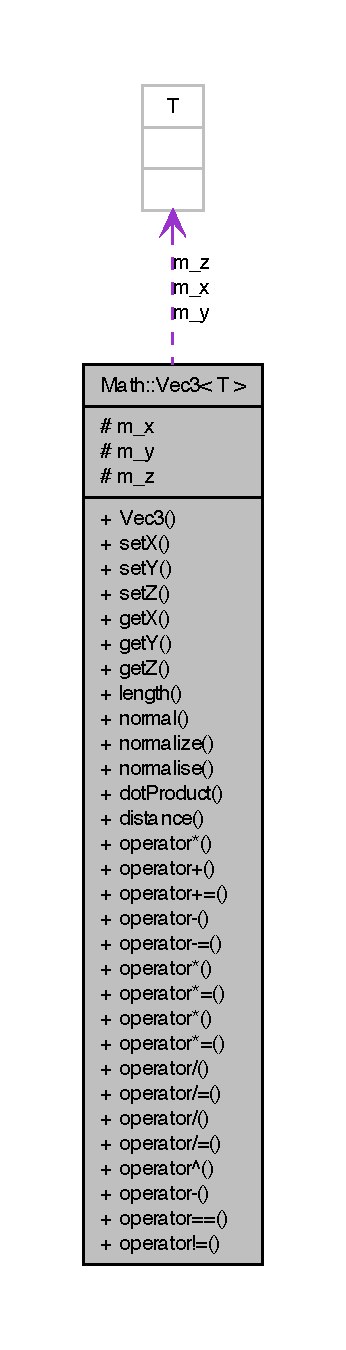
\includegraphics[height=600pt]{class_math_1_1_vec3__coll__graph}
\end{center}
\end{figure}
\subsection*{Public Member Functions}
\begin{DoxyCompactItemize}
\item 
\hyperlink{class_math_1_1_vec3_aecaea0693c6d31b1df4f4d2d75beb868}{Vec3} (const T \&aX=0, const T \&aY=0, const T \&aZ=0)
\begin{DoxyCompactList}\small\item\em Default Constructor. \end{DoxyCompactList}\item 
void \hyperlink{class_math_1_1_vec3_a5fc8f5b4eb732f0be26f7d90fc40488e}{setX} (const T \&aValue)
\begin{DoxyCompactList}\small\item\em Set the position along the x-\/axis. \end{DoxyCompactList}\item 
void \hyperlink{class_math_1_1_vec3_aa0aad7c28629148a5e9c587018f77dea}{setY} (const T \&aValue)
\begin{DoxyCompactList}\small\item\em Set the position along the y-\/axis. \end{DoxyCompactList}\item 
void \hyperlink{class_math_1_1_vec3_a567e7b6e9cd6bdf618b809c39f8103ef}{setZ} (const T \&aValue)
\begin{DoxyCompactList}\small\item\em Set the position along the z-\/axis. \end{DoxyCompactList}\item 
T \hyperlink{class_math_1_1_vec3_a0e6a0ae44f04152b422347026a0fd1de}{getX} () const 
\begin{DoxyCompactList}\small\item\em Accessor on the position along the x-\/axis. \end{DoxyCompactList}\item 
T \hyperlink{class_math_1_1_vec3_a80aed59b26dc66cc526a8b90d60243d3}{getY} () const 
\begin{DoxyCompactList}\small\item\em Accessor on the position along the y-\/axis. \end{DoxyCompactList}\item 
T \hyperlink{class_math_1_1_vec3_a644d7ca5de8c43849d192a47aebc1def}{getZ} () const 
\begin{DoxyCompactList}\small\item\em Accessor on the position along the z-\/axis. \end{DoxyCompactList}\item 
double \hyperlink{class_math_1_1_vec3_ac08670872d34c04db0643b20051aa2a6}{length} () const 
\begin{DoxyCompactList}\small\item\em Get the length of the vector. \end{DoxyCompactList}\item 
\hyperlink{class_math_1_1_vec3}{Vec3} \hyperlink{class_math_1_1_vec3_a7c297a2db8e2d2c8d96626e1f037c506}{normal} () const 
\begin{DoxyCompactList}\small\item\em Get the unit vector corresponding to the normed current vector. \end{DoxyCompactList}\item 
void \hyperlink{class_math_1_1_vec3_aac516bf8cf2b0abe1d96c32ae83644d0}{normalize} ()
\begin{DoxyCompactList}\small\item\em Normalize the current vector so that its length is 1. \end{DoxyCompactList}\item 
void \hyperlink{class_math_1_1_vec3_a6abaf3935a4507648c492d1fe90d4dc7}{normalise} ()
\begin{DoxyCompactList}\small\item\em Normalise the current vector so that its length is 1. \end{DoxyCompactList}\item 
double \hyperlink{class_math_1_1_vec3_ae4fa4fabd84a4711c9494872a6593495}{dotProduct} (const \hyperlink{class_math_1_1_vec3}{Vec3} \&aVector) const 
\begin{DoxyCompactList}\small\item\em Get the dot product between the current vector and a given vector. \end{DoxyCompactList}\item 
double \hyperlink{class_math_1_1_vec3_a5aab62e1729b0e27b544cfd5c89cc0f4}{distance} (const \hyperlink{class_math_1_1_vec3}{Vec3} \&aVector) const 
\item 
double \hyperlink{class_math_1_1_vec3_af4e46f39f829553745000a725f6b946a}{operator$\ast$} (const \hyperlink{class_math_1_1_vec3}{Vec3} \&aVector) const 
\item 
const \hyperlink{class_math_1_1_vec3}{Vec3} \hyperlink{class_math_1_1_vec3_a99eea813a1772346fbd86699eee96508}{operator+} (const \hyperlink{class_math_1_1_vec3}{Vec3} \&aVector) const 
\begin{DoxyCompactList}\small\item\em Operator +. \end{DoxyCompactList}\item 
\hyperlink{class_math_1_1_vec3}{Vec3} \& \hyperlink{class_math_1_1_vec3_a1c558bd3744c7f5184267d5b72e7b356}{operator+=} (const \hyperlink{class_math_1_1_vec3}{Vec3} \&aVector)
\begin{DoxyCompactList}\small\item\em Operator +=. \end{DoxyCompactList}\item 
const \hyperlink{class_math_1_1_vec3}{Vec3} \hyperlink{class_math_1_1_vec3_a5f3ea1c937cb3a920eb9c4052df155db}{operator-\/} (const \hyperlink{class_math_1_1_vec3}{Vec3} \&aVector) const 
\begin{DoxyCompactList}\small\item\em Operator -\/. \end{DoxyCompactList}\item 
\hyperlink{class_math_1_1_vec3}{Vec3} \& \hyperlink{class_math_1_1_vec3_adc2db7214b9e70e71b953abbcc8e202b}{operator-\/=} (const \hyperlink{class_math_1_1_vec3}{Vec3} \&aVector)
\begin{DoxyCompactList}\small\item\em Operator -\/=. \end{DoxyCompactList}\item 
const \hyperlink{class_math_1_1_vec3}{Vec3} \hyperlink{class_math_1_1_vec3_a95c1535c1a95edcaba9d09aa4131c5cb}{operator$\ast$} (const double \&aValue) const 
\begin{DoxyCompactList}\small\item\em Operator $\ast$ to multiply each component of the vector by a given value. \end{DoxyCompactList}\item 
\hyperlink{class_math_1_1_vec3}{Vec3} \& \hyperlink{class_math_1_1_vec3_a4c6c9c61419433e5b48aea9868daaa65}{operator$\ast$=} (const double \&aValue)
\item 
const \hyperlink{class_math_1_1_vec3}{Vec3} \hyperlink{class_math_1_1_vec3_a21d4315f14832a75c6c5234eb53d0018}{operator$\ast$} (const float \&aValue) const 
\begin{DoxyCompactList}\small\item\em Operator $\ast$ to multiply each component of the vector by a given value. \end{DoxyCompactList}\item 
\hyperlink{class_math_1_1_vec3}{Vec3} \& \hyperlink{class_math_1_1_vec3_a478a1fc0ef190230d112fde763a5aec5}{operator$\ast$=} (const float \&aValue)
\item 
const \hyperlink{class_math_1_1_vec3}{Vec3} \hyperlink{class_math_1_1_vec3_a6fefb99be30180f1ba0bf28650dab021}{operator/} (const double \&aValue) const 
\begin{DoxyCompactList}\small\item\em Operator / to divide each component of the vector by a given value. \end{DoxyCompactList}\item 
\hyperlink{class_math_1_1_vec3}{Vec3} \& \hyperlink{class_math_1_1_vec3_a94a0ad94c50a92e7df4ef2eaa80b646d}{operator/=} (const double \&aValue)
\begin{DoxyCompactList}\small\item\em Operator -\/=. \end{DoxyCompactList}\item 
const \hyperlink{class_math_1_1_vec3}{Vec3} \hyperlink{class_math_1_1_vec3_a7b6edfec60d0610b207468266cef5f62}{operator/} (const float \&aValue) const 
\begin{DoxyCompactList}\small\item\em Operator / to divide each component of the vector by a given value. \end{DoxyCompactList}\item 
\hyperlink{class_math_1_1_vec3}{Vec3} \& \hyperlink{class_math_1_1_vec3_a133821008073a67584bf7efe5996222a}{operator/=} (const float \&aValue)
\begin{DoxyCompactList}\small\item\em Operator -\/=. \end{DoxyCompactList}\item 
const \hyperlink{class_math_1_1_vec3}{Vec3} \hyperlink{class_math_1_1_vec3_a3d2915ed100ea1cb23835fc6face8463}{operator$^\wedge$} (const \hyperlink{class_math_1_1_vec3}{Vec3} \&aVector) const 
\item 
const \hyperlink{class_math_1_1_vec3}{Vec3} \hyperlink{class_math_1_1_vec3_ad28e2086bad77ee4d341b8afa1590ca5}{operator-\/} () const 
\begin{DoxyCompactList}\small\item\em Operator -\/ to get the opposite vector. \end{DoxyCompactList}\item 
bool \hyperlink{class_math_1_1_vec3_a59cf913584768084bc2a557b230f2832}{operator==} (const \hyperlink{class_math_1_1_vec3}{Vec3} \&aVector) const 
\begin{DoxyCompactList}\small\item\em Operator ==. \end{DoxyCompactList}\item 
bool \hyperlink{class_math_1_1_vec3_afeec0386f8d8c80c93476e317cf4442e}{operator!=} (const \hyperlink{class_math_1_1_vec3}{Vec3} \&aVector) const 
\begin{DoxyCompactList}\small\item\em Operator !=. \end{DoxyCompactList}\end{DoxyCompactItemize}
\subsection*{Protected Attributes}
\begin{DoxyCompactItemize}
\item 
T \hyperlink{class_math_1_1_vec3_ae5fc08da4fa89bade8c10a0d21458e3d}{m\_\-x}
\begin{DoxyCompactList}\small\item\em the position along the x-\/axis \end{DoxyCompactList}\item 
T \hyperlink{class_math_1_1_vec3_adf02f4fd76cc025b128490a011f50702}{m\_\-y}
\begin{DoxyCompactList}\small\item\em the position along the y-\/axi \end{DoxyCompactList}\item 
T \hyperlink{class_math_1_1_vec3_ae10650a6e5374095a3f35e53c9364c2b}{m\_\-z}
\begin{DoxyCompactList}\small\item\em the position along the z-\/axi \end{DoxyCompactList}\end{DoxyCompactItemize}


\subsection{Detailed Description}
\subsubsection*{template$<$typename T$>$class Math::Vec3$<$ T $>$}

\hyperlink{class_math_1_1_vec3}{Vec3} is a template class to handle a 3D vector. 

Definition at line 67 of file Vec3.h.



\subsection{Constructor \& Destructor Documentation}
\hypertarget{class_math_1_1_vec3_aecaea0693c6d31b1df4f4d2d75beb868}{
\index{Math::Vec3@{Math::Vec3}!Vec3@{Vec3}}
\index{Vec3@{Vec3}!Math::Vec3@{Math::Vec3}}
\subsubsection[{Vec3}]{\setlength{\rightskip}{0pt plus 5cm}template$<$typename T$>$ {\bf Math::Vec3}$<$ T $>$::{\bf Vec3} (
\begin{DoxyParamCaption}
\item[{const T \&}]{aX = {\ttfamily 0}, }
\item[{const T \&}]{aY = {\ttfamily 0}, }
\item[{const T \&}]{aZ = {\ttfamily 0}}
\end{DoxyParamCaption}
)}}
\label{class_math_1_1_vec3_aecaea0693c6d31b1df4f4d2d75beb868}


Default Constructor. 


\begin{DoxyParams}{Parameters}
{\em aX,:} & the position along the x-\/axis (default value is 0) \\
\hline
{\em aY,:} & the position along the y-\/axis (default value is 0) \\
\hline
{\em aZ,:} & the position along the z-\/axis (default value is 0) \\
\hline
\end{DoxyParams}


Definition at line 42 of file Vec3.inl.



\subsection{Member Function Documentation}
\hypertarget{class_math_1_1_vec3_a5aab62e1729b0e27b544cfd5c89cc0f4}{
\index{Math::Vec3@{Math::Vec3}!distance@{distance}}
\index{distance@{distance}!Math::Vec3@{Math::Vec3}}
\subsubsection[{distance}]{\setlength{\rightskip}{0pt plus 5cm}template$<$typename T $>$ double {\bf Math::Vec3}$<$ T $>$::distance (
\begin{DoxyParamCaption}
\item[{const {\bf Vec3}$<$ T $>$ \&}]{aVector}
\end{DoxyParamCaption}
) const}}
\label{class_math_1_1_vec3_a5aab62e1729b0e27b544cfd5c89cc0f4}
Get the distance between the 3D position represented by the current vector and another position. 
\begin{DoxyParams}{Parameters}
{\em aVector,:} & the other vector \\
\hline
\end{DoxyParams}
\begin{DoxyReturn}{Returns}
the distance 
\end{DoxyReturn}


Definition at line 151 of file Vec3.inl.

\hypertarget{class_math_1_1_vec3_ae4fa4fabd84a4711c9494872a6593495}{
\index{Math::Vec3@{Math::Vec3}!dotProduct@{dotProduct}}
\index{dotProduct@{dotProduct}!Math::Vec3@{Math::Vec3}}
\subsubsection[{dotProduct}]{\setlength{\rightskip}{0pt plus 5cm}template$<$typename T $>$ double {\bf Math::Vec3}$<$ T $>$::dotProduct (
\begin{DoxyParamCaption}
\item[{const {\bf Vec3}$<$ T $>$ \&}]{aVector}
\end{DoxyParamCaption}
) const}}
\label{class_math_1_1_vec3_ae4fa4fabd84a4711c9494872a6593495}


Get the dot product between the current vector and a given vector. 


\begin{DoxyParams}{Parameters}
{\em aVector,:} & the other vector \\
\hline
\end{DoxyParams}
\begin{DoxyReturn}{Returns}
the dot product 
\end{DoxyReturn}


Definition at line 135 of file Vec3.inl.

\hypertarget{class_math_1_1_vec3_a0e6a0ae44f04152b422347026a0fd1de}{
\index{Math::Vec3@{Math::Vec3}!getX@{getX}}
\index{getX@{getX}!Math::Vec3@{Math::Vec3}}
\subsubsection[{getX}]{\setlength{\rightskip}{0pt plus 5cm}template$<$typename T $>$ T {\bf Math::Vec3}$<$ T $>$::getX (
\begin{DoxyParamCaption}
{}
\end{DoxyParamCaption}
) const}}
\label{class_math_1_1_vec3_a0e6a0ae44f04152b422347026a0fd1de}


Accessor on the position along the x-\/axis. 

\begin{DoxyReturn}{Returns}
the position along the x-\/axis 
\end{DoxyReturn}


Definition at line 76 of file Vec3.inl.

\hypertarget{class_math_1_1_vec3_a80aed59b26dc66cc526a8b90d60243d3}{
\index{Math::Vec3@{Math::Vec3}!getY@{getY}}
\index{getY@{getY}!Math::Vec3@{Math::Vec3}}
\subsubsection[{getY}]{\setlength{\rightskip}{0pt plus 5cm}template$<$typename T $>$ T {\bf Math::Vec3}$<$ T $>$::getY (
\begin{DoxyParamCaption}
{}
\end{DoxyParamCaption}
) const}}
\label{class_math_1_1_vec3_a80aed59b26dc66cc526a8b90d60243d3}


Accessor on the position along the y-\/axis. 

\begin{DoxyReturn}{Returns}
the position along the y-\/axis 
\end{DoxyReturn}


Definition at line 84 of file Vec3.inl.

\hypertarget{class_math_1_1_vec3_a644d7ca5de8c43849d192a47aebc1def}{
\index{Math::Vec3@{Math::Vec3}!getZ@{getZ}}
\index{getZ@{getZ}!Math::Vec3@{Math::Vec3}}
\subsubsection[{getZ}]{\setlength{\rightskip}{0pt plus 5cm}template$<$typename T $>$ T {\bf Math::Vec3}$<$ T $>$::getZ (
\begin{DoxyParamCaption}
{}
\end{DoxyParamCaption}
) const}}
\label{class_math_1_1_vec3_a644d7ca5de8c43849d192a47aebc1def}


Accessor on the position along the z-\/axis. 

\begin{DoxyReturn}{Returns}
the position along the z-\/axis 
\end{DoxyReturn}


Definition at line 92 of file Vec3.inl.

\hypertarget{class_math_1_1_vec3_ac08670872d34c04db0643b20051aa2a6}{
\index{Math::Vec3@{Math::Vec3}!length@{length}}
\index{length@{length}!Math::Vec3@{Math::Vec3}}
\subsubsection[{length}]{\setlength{\rightskip}{0pt plus 5cm}template$<$typename T $>$ double {\bf Math::Vec3}$<$ T $>$::length (
\begin{DoxyParamCaption}
{}
\end{DoxyParamCaption}
) const}}
\label{class_math_1_1_vec3_ac08670872d34c04db0643b20051aa2a6}


Get the length of the vector. 

\begin{DoxyReturn}{Returns}
the length of the vector 
\end{DoxyReturn}


Definition at line 100 of file Vec3.inl.

\hypertarget{class_math_1_1_vec3_a7c297a2db8e2d2c8d96626e1f037c506}{
\index{Math::Vec3@{Math::Vec3}!normal@{normal}}
\index{normal@{normal}!Math::Vec3@{Math::Vec3}}
\subsubsection[{normal}]{\setlength{\rightskip}{0pt plus 5cm}template$<$typename T $>$ {\bf Vec3}$<$ T $>$ {\bf Math::Vec3}$<$ T $>$::normal (
\begin{DoxyParamCaption}
{}
\end{DoxyParamCaption}
) const}}
\label{class_math_1_1_vec3_a7c297a2db8e2d2c8d96626e1f037c506}


Get the unit vector corresponding to the normed current vector. 

\begin{DoxyReturn}{Returns}
the unit vector 
\end{DoxyReturn}


Definition at line 108 of file Vec3.inl.

\hypertarget{class_math_1_1_vec3_a6abaf3935a4507648c492d1fe90d4dc7}{
\index{Math::Vec3@{Math::Vec3}!normalise@{normalise}}
\index{normalise@{normalise}!Math::Vec3@{Math::Vec3}}
\subsubsection[{normalise}]{\setlength{\rightskip}{0pt plus 5cm}template$<$typename T $>$ void {\bf Math::Vec3}$<$ T $>$::normalise (
\begin{DoxyParamCaption}
{}
\end{DoxyParamCaption}
)}}
\label{class_math_1_1_vec3_a6abaf3935a4507648c492d1fe90d4dc7}


Normalise the current vector so that its length is 1. 



Definition at line 127 of file Vec3.inl.

\hypertarget{class_math_1_1_vec3_aac516bf8cf2b0abe1d96c32ae83644d0}{
\index{Math::Vec3@{Math::Vec3}!normalize@{normalize}}
\index{normalize@{normalize}!Math::Vec3@{Math::Vec3}}
\subsubsection[{normalize}]{\setlength{\rightskip}{0pt plus 5cm}template$<$typename T $>$ void {\bf Math::Vec3}$<$ T $>$::normalize (
\begin{DoxyParamCaption}
{}
\end{DoxyParamCaption}
)}}
\label{class_math_1_1_vec3_aac516bf8cf2b0abe1d96c32ae83644d0}


Normalize the current vector so that its length is 1. 



Definition at line 116 of file Vec3.inl.

\hypertarget{class_math_1_1_vec3_afeec0386f8d8c80c93476e317cf4442e}{
\index{Math::Vec3@{Math::Vec3}!operator!=@{operator!=}}
\index{operator!=@{operator!=}!Math::Vec3@{Math::Vec3}}
\subsubsection[{operator!=}]{\setlength{\rightskip}{0pt plus 5cm}template$<$typename T $>$ bool {\bf Math::Vec3}$<$ T $>$::operator!= (
\begin{DoxyParamCaption}
\item[{const {\bf Vec3}$<$ T $>$ \&}]{aVector}
\end{DoxyParamCaption}
) const}}
\label{class_math_1_1_vec3_afeec0386f8d8c80c93476e317cf4442e}


Operator !=. 


\begin{DoxyParams}{Parameters}
{\em aVector,:} & the vector to compare the current vector with \\
\hline
\end{DoxyParams}
\begin{DoxyReturn}{Returns}
true if the two vectors are different, false if the two vectors are the same 
\end{DoxyReturn}


Definition at line 313 of file Vec3.inl.

\hypertarget{class_math_1_1_vec3_a95c1535c1a95edcaba9d09aa4131c5cb}{
\index{Math::Vec3@{Math::Vec3}!operator$\ast$@{operator$\ast$}}
\index{operator$\ast$@{operator$\ast$}!Math::Vec3@{Math::Vec3}}
\subsubsection[{operator$\ast$}]{\setlength{\rightskip}{0pt plus 5cm}template$<$typename T $>$ const {\bf Vec3}$<$ T $>$ {\bf Math::Vec3}$<$ T $>$::operator$\ast$ (
\begin{DoxyParamCaption}
\item[{const double \&}]{aValue}
\end{DoxyParamCaption}
) const}}
\label{class_math_1_1_vec3_a95c1535c1a95edcaba9d09aa4131c5cb}


Operator $\ast$ to multiply each component of the vector by a given value. 


\begin{DoxyParams}{Parameters}
{\em aValue,:} & the multiplicative value \\
\hline
\end{DoxyParams}
\begin{DoxyReturn}{Returns}
the modified vector 
\end{DoxyReturn}


Definition at line 203 of file Vec3.inl.

\hypertarget{class_math_1_1_vec3_a21d4315f14832a75c6c5234eb53d0018}{
\index{Math::Vec3@{Math::Vec3}!operator$\ast$@{operator$\ast$}}
\index{operator$\ast$@{operator$\ast$}!Math::Vec3@{Math::Vec3}}
\subsubsection[{operator$\ast$}]{\setlength{\rightskip}{0pt plus 5cm}template$<$typename T $>$ const {\bf Vec3}$<$ T $>$ {\bf Math::Vec3}$<$ T $>$::operator$\ast$ (
\begin{DoxyParamCaption}
\item[{const float \&}]{aValue}
\end{DoxyParamCaption}
) const}}
\label{class_math_1_1_vec3_a21d4315f14832a75c6c5234eb53d0018}


Operator $\ast$ to multiply each component of the vector by a given value. 


\begin{DoxyParams}{Parameters}
{\em aValue,:} & the multiplicative value \\
\hline
\end{DoxyParams}
\begin{DoxyReturn}{Returns}
the modified vector 
\end{DoxyReturn}


Definition at line 223 of file Vec3.inl.

\hypertarget{class_math_1_1_vec3_af4e46f39f829553745000a725f6b946a}{
\index{Math::Vec3@{Math::Vec3}!operator$\ast$@{operator$\ast$}}
\index{operator$\ast$@{operator$\ast$}!Math::Vec3@{Math::Vec3}}
\subsubsection[{operator$\ast$}]{\setlength{\rightskip}{0pt plus 5cm}template$<$typename T $>$ double {\bf Math::Vec3}$<$ T $>$::operator$\ast$ (
\begin{DoxyParamCaption}
\item[{const {\bf Vec3}$<$ T $>$ \&}]{aVector}
\end{DoxyParamCaption}
) const}}
\label{class_math_1_1_vec3_af4e46f39f829553745000a725f6b946a}
Operator $\ast$ to compute the dot product between the current vector and a given vector. 
\begin{DoxyParams}{Parameters}
{\em aVector,:} & the other vector \\
\hline
\end{DoxyParams}
\begin{DoxyReturn}{Returns}
the dot product 
\end{DoxyReturn}


Definition at line 143 of file Vec3.inl.

\hypertarget{class_math_1_1_vec3_a4c6c9c61419433e5b48aea9868daaa65}{
\index{Math::Vec3@{Math::Vec3}!operator$\ast$=@{operator$\ast$=}}
\index{operator$\ast$=@{operator$\ast$=}!Math::Vec3@{Math::Vec3}}
\subsubsection[{operator$\ast$=}]{\setlength{\rightskip}{0pt plus 5cm}template$<$typename T $>$ {\bf Vec3}$<$ T $>$ \& {\bf Math::Vec3}$<$ T $>$::operator$\ast$= (
\begin{DoxyParamCaption}
\item[{const double \&}]{aValue}
\end{DoxyParamCaption}
)}}
\label{class_math_1_1_vec3_a4c6c9c61419433e5b48aea9868daaa65}
Operator $\ast$= to multiply each component of the vector by a given value, and modify the current vector. 
\begin{DoxyParams}{Parameters}
{\em aValue,:} & the multiplicative value \\
\hline
\end{DoxyParams}
\begin{DoxyReturn}{Returns}
the modified vector 
\end{DoxyReturn}


Definition at line 211 of file Vec3.inl.

\hypertarget{class_math_1_1_vec3_a478a1fc0ef190230d112fde763a5aec5}{
\index{Math::Vec3@{Math::Vec3}!operator$\ast$=@{operator$\ast$=}}
\index{operator$\ast$=@{operator$\ast$=}!Math::Vec3@{Math::Vec3}}
\subsubsection[{operator$\ast$=}]{\setlength{\rightskip}{0pt plus 5cm}template$<$typename T $>$ {\bf Vec3}$<$ T $>$ \& {\bf Math::Vec3}$<$ T $>$::operator$\ast$= (
\begin{DoxyParamCaption}
\item[{const float \&}]{aValue}
\end{DoxyParamCaption}
)}}
\label{class_math_1_1_vec3_a478a1fc0ef190230d112fde763a5aec5}
Operator $\ast$= to multiply each component of the vector by a given value, and modify the current vector. 
\begin{DoxyParams}{Parameters}
{\em aValue,:} & the multiplicative value \\
\hline
\end{DoxyParams}
\begin{DoxyReturn}{Returns}
the modified vector 
\end{DoxyReturn}


Definition at line 231 of file Vec3.inl.

\hypertarget{class_math_1_1_vec3_a99eea813a1772346fbd86699eee96508}{
\index{Math::Vec3@{Math::Vec3}!operator+@{operator+}}
\index{operator+@{operator+}!Math::Vec3@{Math::Vec3}}
\subsubsection[{operator+}]{\setlength{\rightskip}{0pt plus 5cm}template$<$typename T $>$ const {\bf Vec3}$<$ T $>$ {\bf Math::Vec3}$<$ T $>$::operator+ (
\begin{DoxyParamCaption}
\item[{const {\bf Vec3}$<$ T $>$ \&}]{aVector}
\end{DoxyParamCaption}
) const}}
\label{class_math_1_1_vec3_a99eea813a1772346fbd86699eee96508}


Operator +. 


\begin{DoxyParams}{Parameters}
{\em aVector,:} & the other vector \\
\hline
\end{DoxyParams}
\begin{DoxyReturn}{Returns}
the dot product 
\end{DoxyReturn}


Definition at line 163 of file Vec3.inl.

\hypertarget{class_math_1_1_vec3_a1c558bd3744c7f5184267d5b72e7b356}{
\index{Math::Vec3@{Math::Vec3}!operator+=@{operator+=}}
\index{operator+=@{operator+=}!Math::Vec3@{Math::Vec3}}
\subsubsection[{operator+=}]{\setlength{\rightskip}{0pt plus 5cm}template$<$typename T $>$ {\bf Vec3}$<$ T $>$ \& {\bf Math::Vec3}$<$ T $>$::operator+= (
\begin{DoxyParamCaption}
\item[{const {\bf Vec3}$<$ T $>$ \&}]{aVector}
\end{DoxyParamCaption}
)}}
\label{class_math_1_1_vec3_a1c558bd3744c7f5184267d5b72e7b356}


Operator +=. 


\begin{DoxyParams}{Parameters}
{\em aVector,:} & the other vector \\
\hline
\end{DoxyParams}
\begin{DoxyReturn}{Returns}
the modified vector 
\end{DoxyReturn}


Definition at line 171 of file Vec3.inl.

\hypertarget{class_math_1_1_vec3_a5f3ea1c937cb3a920eb9c4052df155db}{
\index{Math::Vec3@{Math::Vec3}!operator-\/@{operator-\/}}
\index{operator-\/@{operator-\/}!Math::Vec3@{Math::Vec3}}
\subsubsection[{operator-\/}]{\setlength{\rightskip}{0pt plus 5cm}template$<$typename T $>$ const {\bf Vec3}$<$ T $>$ {\bf Math::Vec3}$<$ T $>$::operator-\/ (
\begin{DoxyParamCaption}
\item[{const {\bf Vec3}$<$ T $>$ \&}]{aVector}
\end{DoxyParamCaption}
) const}}
\label{class_math_1_1_vec3_a5f3ea1c937cb3a920eb9c4052df155db}


Operator -\/. 


\begin{DoxyParams}{Parameters}
{\em aVector,:} & the other vector \\
\hline
\end{DoxyParams}
\begin{DoxyReturn}{Returns}
the modified vector 
\end{DoxyReturn}


Definition at line 183 of file Vec3.inl.

\hypertarget{class_math_1_1_vec3_ad28e2086bad77ee4d341b8afa1590ca5}{
\index{Math::Vec3@{Math::Vec3}!operator-\/@{operator-\/}}
\index{operator-\/@{operator-\/}!Math::Vec3@{Math::Vec3}}
\subsubsection[{operator-\/}]{\setlength{\rightskip}{0pt plus 5cm}template$<$typename T $>$ const {\bf Vec3}$<$ T $>$ {\bf Math::Vec3}$<$ T $>$::operator-\/ (
\begin{DoxyParamCaption}
{}
\end{DoxyParamCaption}
) const}}
\label{class_math_1_1_vec3_ad28e2086bad77ee4d341b8afa1590ca5}


Operator -\/ to get the opposite vector. 

\begin{DoxyReturn}{Returns}
the opposite vector 
\end{DoxyReturn}


Definition at line 293 of file Vec3.inl.

\hypertarget{class_math_1_1_vec3_adc2db7214b9e70e71b953abbcc8e202b}{
\index{Math::Vec3@{Math::Vec3}!operator-\/=@{operator-\/=}}
\index{operator-\/=@{operator-\/=}!Math::Vec3@{Math::Vec3}}
\subsubsection[{operator-\/=}]{\setlength{\rightskip}{0pt plus 5cm}template$<$typename T $>$ {\bf Vec3}$<$ T $>$ \& {\bf Math::Vec3}$<$ T $>$::operator-\/= (
\begin{DoxyParamCaption}
\item[{const {\bf Vec3}$<$ T $>$ \&}]{aVector}
\end{DoxyParamCaption}
)}}
\label{class_math_1_1_vec3_adc2db7214b9e70e71b953abbcc8e202b}


Operator -\/=. 


\begin{DoxyParams}{Parameters}
{\em aVector,:} & the other vector \\
\hline
\end{DoxyParams}
\begin{DoxyReturn}{Returns}
the modified vector 
\end{DoxyReturn}


Definition at line 191 of file Vec3.inl.

\hypertarget{class_math_1_1_vec3_a6fefb99be30180f1ba0bf28650dab021}{
\index{Math::Vec3@{Math::Vec3}!operator/@{operator/}}
\index{operator/@{operator/}!Math::Vec3@{Math::Vec3}}
\subsubsection[{operator/}]{\setlength{\rightskip}{0pt plus 5cm}template$<$typename T $>$ const {\bf Vec3}$<$ T $>$ {\bf Math::Vec3}$<$ T $>$::operator/ (
\begin{DoxyParamCaption}
\item[{const double \&}]{aValue}
\end{DoxyParamCaption}
) const}}
\label{class_math_1_1_vec3_a6fefb99be30180f1ba0bf28650dab021}


Operator / to divide each component of the vector by a given value. 


\begin{DoxyParams}{Parameters}
{\em aValue,:} & the value \\
\hline
\end{DoxyParams}
\begin{DoxyReturn}{Returns}
the modified vector 
\end{DoxyReturn}


Definition at line 243 of file Vec3.inl.

\hypertarget{class_math_1_1_vec3_a7b6edfec60d0610b207468266cef5f62}{
\index{Math::Vec3@{Math::Vec3}!operator/@{operator/}}
\index{operator/@{operator/}!Math::Vec3@{Math::Vec3}}
\subsubsection[{operator/}]{\setlength{\rightskip}{0pt plus 5cm}template$<$typename T $>$ const {\bf Vec3}$<$ T $>$ {\bf Math::Vec3}$<$ T $>$::operator/ (
\begin{DoxyParamCaption}
\item[{const float \&}]{aValue}
\end{DoxyParamCaption}
) const}}
\label{class_math_1_1_vec3_a7b6edfec60d0610b207468266cef5f62}


Operator / to divide each component of the vector by a given value. 


\begin{DoxyParams}{Parameters}
{\em aValue,:} & the value \\
\hline
\end{DoxyParams}
\begin{DoxyReturn}{Returns}
the modified vector 
\end{DoxyReturn}


Definition at line 263 of file Vec3.inl.

\hypertarget{class_math_1_1_vec3_a94a0ad94c50a92e7df4ef2eaa80b646d}{
\index{Math::Vec3@{Math::Vec3}!operator/=@{operator/=}}
\index{operator/=@{operator/=}!Math::Vec3@{Math::Vec3}}
\subsubsection[{operator/=}]{\setlength{\rightskip}{0pt plus 5cm}template$<$typename T $>$ {\bf Vec3}$<$ T $>$ \& {\bf Math::Vec3}$<$ T $>$::operator/= (
\begin{DoxyParamCaption}
\item[{const double \&}]{aValue}
\end{DoxyParamCaption}
)}}
\label{class_math_1_1_vec3_a94a0ad94c50a92e7df4ef2eaa80b646d}


Operator -\/=. 


\begin{DoxyParams}{Parameters}
{\em aValue,:} & the other vector \\
\hline
\end{DoxyParams}
\begin{DoxyReturn}{Returns}
the modified vector 
\end{DoxyReturn}


Definition at line 251 of file Vec3.inl.

\hypertarget{class_math_1_1_vec3_a133821008073a67584bf7efe5996222a}{
\index{Math::Vec3@{Math::Vec3}!operator/=@{operator/=}}
\index{operator/=@{operator/=}!Math::Vec3@{Math::Vec3}}
\subsubsection[{operator/=}]{\setlength{\rightskip}{0pt plus 5cm}template$<$typename T $>$ {\bf Vec3}$<$ T $>$ \& {\bf Math::Vec3}$<$ T $>$::operator/= (
\begin{DoxyParamCaption}
\item[{const float \&}]{aValue}
\end{DoxyParamCaption}
)}}
\label{class_math_1_1_vec3_a133821008073a67584bf7efe5996222a}


Operator -\/=. 


\begin{DoxyParams}{Parameters}
{\em aValue,:} & the other vector \\
\hline
\end{DoxyParams}
\begin{DoxyReturn}{Returns}
the modified vector 
\end{DoxyReturn}


Definition at line 271 of file Vec3.inl.

\hypertarget{class_math_1_1_vec3_a59cf913584768084bc2a557b230f2832}{
\index{Math::Vec3@{Math::Vec3}!operator==@{operator==}}
\index{operator==@{operator==}!Math::Vec3@{Math::Vec3}}
\subsubsection[{operator==}]{\setlength{\rightskip}{0pt plus 5cm}template$<$typename T $>$ bool {\bf Math::Vec3}$<$ T $>$::operator== (
\begin{DoxyParamCaption}
\item[{const {\bf Vec3}$<$ T $>$ \&}]{aVector}
\end{DoxyParamCaption}
) const}}
\label{class_math_1_1_vec3_a59cf913584768084bc2a557b230f2832}


Operator ==. 


\begin{DoxyParams}{Parameters}
{\em aVector,:} & the vector to compare the current vector with \\
\hline
\end{DoxyParams}
\begin{DoxyReturn}{Returns}
true if the two vectors are the same, false if the two vectors are different 
\end{DoxyReturn}


Definition at line 301 of file Vec3.inl.

\hypertarget{class_math_1_1_vec3_a3d2915ed100ea1cb23835fc6face8463}{
\index{Math::Vec3@{Math::Vec3}!operator$^\wedge$@{operator$^\wedge$}}
\index{operator$^\wedge$@{operator$^\wedge$}!Math::Vec3@{Math::Vec3}}
\subsubsection[{operator$^\wedge$}]{\setlength{\rightskip}{0pt plus 5cm}template$<$typename T $>$ const {\bf Vec3}$<$ T $>$ {\bf Math::Vec3}$<$ T $>$::operator$^\wedge$ (
\begin{DoxyParamCaption}
\item[{const {\bf Vec3}$<$ T $>$ \&}]{aVector}
\end{DoxyParamCaption}
) const}}
\label{class_math_1_1_vec3_a3d2915ed100ea1cb23835fc6face8463}
Operator $^\wedge$ to compute the cross product between the current vector and a given vector. 
\begin{DoxyParams}{Parameters}
{\em aVector,:} & the other vector \\
\hline
\end{DoxyParams}
\begin{DoxyReturn}{Returns}
the cross product 
\end{DoxyReturn}


Definition at line 283 of file Vec3.inl.

\hypertarget{class_math_1_1_vec3_a5fc8f5b4eb732f0be26f7d90fc40488e}{
\index{Math::Vec3@{Math::Vec3}!setX@{setX}}
\index{setX@{setX}!Math::Vec3@{Math::Vec3}}
\subsubsection[{setX}]{\setlength{\rightskip}{0pt plus 5cm}template$<$typename T$>$ void {\bf Math::Vec3}$<$ T $>$::setX (
\begin{DoxyParamCaption}
\item[{const T \&}]{aValue}
\end{DoxyParamCaption}
)}}
\label{class_math_1_1_vec3_a5fc8f5b4eb732f0be26f7d90fc40488e}


Set the position along the x-\/axis. 


\begin{DoxyParams}{Parameters}
{\em aValue,:} & the position along the x-\/axis \\
\hline
\end{DoxyParams}


Definition at line 52 of file Vec3.inl.

\hypertarget{class_math_1_1_vec3_aa0aad7c28629148a5e9c587018f77dea}{
\index{Math::Vec3@{Math::Vec3}!setY@{setY}}
\index{setY@{setY}!Math::Vec3@{Math::Vec3}}
\subsubsection[{setY}]{\setlength{\rightskip}{0pt plus 5cm}template$<$typename T$>$ void {\bf Math::Vec3}$<$ T $>$::setY (
\begin{DoxyParamCaption}
\item[{const T \&}]{aValue}
\end{DoxyParamCaption}
)}}
\label{class_math_1_1_vec3_aa0aad7c28629148a5e9c587018f77dea}


Set the position along the y-\/axis. 


\begin{DoxyParams}{Parameters}
{\em aValue,:} & the position along the y-\/axis \\
\hline
\end{DoxyParams}


Definition at line 60 of file Vec3.inl.

\hypertarget{class_math_1_1_vec3_a567e7b6e9cd6bdf618b809c39f8103ef}{
\index{Math::Vec3@{Math::Vec3}!setZ@{setZ}}
\index{setZ@{setZ}!Math::Vec3@{Math::Vec3}}
\subsubsection[{setZ}]{\setlength{\rightskip}{0pt plus 5cm}template$<$typename T$>$ void {\bf Math::Vec3}$<$ T $>$::setZ (
\begin{DoxyParamCaption}
\item[{const T \&}]{aValue}
\end{DoxyParamCaption}
)}}
\label{class_math_1_1_vec3_a567e7b6e9cd6bdf618b809c39f8103ef}


Set the position along the z-\/axis. 


\begin{DoxyParams}{Parameters}
{\em aValue,:} & the position along the z-\/axis \\
\hline
\end{DoxyParams}


Definition at line 68 of file Vec3.inl.



\subsection{Member Data Documentation}
\hypertarget{class_math_1_1_vec3_ae5fc08da4fa89bade8c10a0d21458e3d}{
\index{Math::Vec3@{Math::Vec3}!m\_\-x@{m\_\-x}}
\index{m\_\-x@{m\_\-x}!Math::Vec3@{Math::Vec3}}
\subsubsection[{m\_\-x}]{\setlength{\rightskip}{0pt plus 5cm}template$<$typename T$>$ T {\bf Math::Vec3}$<$ T $>$::{\bf m\_\-x}\hspace{0.3cm}{\ttfamily  \mbox{[}protected\mbox{]}}}}
\label{class_math_1_1_vec3_ae5fc08da4fa89bade8c10a0d21458e3d}


the position along the x-\/axis 



Definition at line 364 of file Vec3.h.

\hypertarget{class_math_1_1_vec3_adf02f4fd76cc025b128490a011f50702}{
\index{Math::Vec3@{Math::Vec3}!m\_\-y@{m\_\-y}}
\index{m\_\-y@{m\_\-y}!Math::Vec3@{Math::Vec3}}
\subsubsection[{m\_\-y}]{\setlength{\rightskip}{0pt plus 5cm}template$<$typename T$>$ T {\bf Math::Vec3}$<$ T $>$::{\bf m\_\-y}\hspace{0.3cm}{\ttfamily  \mbox{[}protected\mbox{]}}}}
\label{class_math_1_1_vec3_adf02f4fd76cc025b128490a011f50702}


the position along the y-\/axi 



Definition at line 365 of file Vec3.h.

\hypertarget{class_math_1_1_vec3_ae10650a6e5374095a3f35e53c9364c2b}{
\index{Math::Vec3@{Math::Vec3}!m\_\-z@{m\_\-z}}
\index{m\_\-z@{m\_\-z}!Math::Vec3@{Math::Vec3}}
\subsubsection[{m\_\-z}]{\setlength{\rightskip}{0pt plus 5cm}template$<$typename T$>$ T {\bf Math::Vec3}$<$ T $>$::{\bf m\_\-z}\hspace{0.3cm}{\ttfamily  \mbox{[}protected\mbox{]}}}}
\label{class_math_1_1_vec3_ae10650a6e5374095a3f35e53c9364c2b}


the position along the z-\/axi 



Definition at line 366 of file Vec3.h.



The documentation for this class was generated from the following files:\begin{DoxyCompactItemize}
\item 
/Users/fpvidal/Documents/gvirtualxray-\/code/trunk/include/gVirtualXRay/\hyperlink{_vec3_8h}{Vec3.h}\item 
/Users/fpvidal/Documents/gvirtualxray-\/code/trunk/include/gVirtualXRay/\hyperlink{_vec3_8inl}{Vec3.inl}\end{DoxyCompactItemize}

\hypertarget{classg_virtual_x_ray_1_1_x_ray_beam}{
\section{gVirtualXRay::XRayBeam Class Reference}
\label{classg_virtual_x_ray_1_1_x_ray_beam}\index{gVirtualXRay::XRayBeam@{gVirtualXRay::XRayBeam}}
}


\hyperlink{classg_virtual_x_ray_1_1_x_ray_beam}{XRayBeam} is a class to handle the X-\/Ray beam. The beam spectrum is discretised into energy channels.  




{\ttfamily \#include $<$XRayBeam.h$>$}

\subsection*{Public Member Functions}
\begin{DoxyCompactItemize}
\item 
\hyperlink{classg_virtual_x_ray_1_1_x_ray_beam_acc2516eafa024fd55c922fda31c05cf1}{XRayBeam} ()
\begin{DoxyCompactList}\small\item\em Default constructor. \end{DoxyCompactList}\item 
void \hyperlink{classg_virtual_x_ray_1_1_x_ray_beam_a8fca507a5d6a8e6c1c9607f0e9ddb1e4}{initialise} (const char $\ast$aFileName, const \hyperlink{namespace_utilities_a40969b96bd8d847b962e297cb79f08ce}{RATIONAL\_\-NUMBER} \&aUnit, unsigned int aMergeChannelFlag=1)
\begin{DoxyCompactList}\small\item\em Initialise the X-\/ray beam specturm with a polychromatic spectrum. \end{DoxyCompactList}\item 
void \hyperlink{classg_virtual_x_ray_1_1_x_ray_beam_a9098d87242fdedd548b87cc6fe1414f9}{initialise} (const \hyperlink{namespace_utilities_a40969b96bd8d847b962e297cb79f08ce}{RATIONAL\_\-NUMBER} \&anIncidentEnergy)
\begin{DoxyCompactList}\small\item\em Initialise the X-\/ray beam specturm with a monochromatic spectrum. \end{DoxyCompactList}\item 
void \hyperlink{classg_virtual_x_ray_1_1_x_ray_beam_a34219da39048ef19cdb984fc7df33ee0}{normalise} ()
\begin{DoxyCompactList}\small\item\em Normalise the number of photons so that the total incident energy is 1.0. \end{DoxyCompactList}\item 
void \hyperlink{classg_virtual_x_ray_1_1_x_ray_beam_a96b9f89afb0b7c5e52c35ad16544364f}{setNumberOfPhotonsLowerThreshold} (const \hyperlink{namespace_utilities_a40969b96bd8d847b962e297cb79f08ce}{RATIONAL\_\-NUMBER} \&aThreshold)
\begin{DoxyCompactList}\small\item\em Set a threshold to discard energy bins with a tiny number of photons. \end{DoxyCompactList}\item 
unsigned int \hyperlink{classg_virtual_x_ray_1_1_x_ray_beam_a80658e6d864130431b2eaed3a5ae9095}{getEnergyChannelNumber} () const 
\begin{DoxyCompactList}\small\item\em Accessor on the number of bins in the spectrum. \end{DoxyCompactList}\item 
const \hyperlink{classg_virtual_x_ray_1_1_spectrum_record}{SpectrumRecord} \& \hyperlink{classg_virtual_x_ray_1_1_x_ray_beam_a1cf7093fc484de7e727f0dd52c1c94f5}{getEnergyChannel} (unsigned int anID) const 
\begin{DoxyCompactList}\small\item\em Accessor on a given energy bin. \end{DoxyCompactList}\end{DoxyCompactItemize}
\subsection*{Protected Attributes}
\begin{DoxyCompactItemize}
\item 
std::vector$<$ \hyperlink{classg_virtual_x_ray_1_1_spectrum_record}{SpectrumRecord} $>$ \hyperlink{classg_virtual_x_ray_1_1_x_ray_beam_a15eeb7ae26c0d69c67d495055b6894ee}{m\_\-beam\_\-spectrum}
\begin{DoxyCompactList}\small\item\em Set of photon bins. \end{DoxyCompactList}\item 
\hyperlink{namespace_utilities_a40969b96bd8d847b962e297cb79f08ce}{RATIONAL\_\-NUMBER} \hyperlink{classg_virtual_x_ray_1_1_x_ray_beam_a700a497bc1f73a3b2e2fc2c3e83bde61}{m\_\-number\_\-of\_\-photons\_\-lower\_\-threshold}
\end{DoxyCompactItemize}


\subsection{Detailed Description}
\hyperlink{classg_virtual_x_ray_1_1_x_ray_beam}{XRayBeam} is a class to handle the X-\/Ray beam. The beam spectrum is discretised into energy channels. 

Definition at line 62 of file XRayBeam.h.



\subsection{Constructor \& Destructor Documentation}
\hypertarget{classg_virtual_x_ray_1_1_x_ray_beam_acc2516eafa024fd55c922fda31c05cf1}{
\index{gVirtualXRay::XRayBeam@{gVirtualXRay::XRayBeam}!XRayBeam@{XRayBeam}}
\index{XRayBeam@{XRayBeam}!gVirtualXRay::XRayBeam@{gVirtualXRay::XRayBeam}}
\subsubsection[{XRayBeam}]{\setlength{\rightskip}{0pt plus 5cm}gVirtualXRay::XRayBeam::XRayBeam (
\begin{DoxyParamCaption}
{}
\end{DoxyParamCaption}
)\hspace{0.3cm}{\ttfamily  \mbox{[}inline\mbox{]}}}}
\label{classg_virtual_x_ray_1_1_x_ray_beam_acc2516eafa024fd55c922fda31c05cf1}


Default constructor. 



Definition at line 53 of file XRayBeam.inl.



\subsection{Member Function Documentation}
\hypertarget{classg_virtual_x_ray_1_1_x_ray_beam_a1cf7093fc484de7e727f0dd52c1c94f5}{
\index{gVirtualXRay::XRayBeam@{gVirtualXRay::XRayBeam}!getEnergyChannel@{getEnergyChannel}}
\index{getEnergyChannel@{getEnergyChannel}!gVirtualXRay::XRayBeam@{gVirtualXRay::XRayBeam}}
\subsubsection[{getEnergyChannel}]{\setlength{\rightskip}{0pt plus 5cm}const {\bf SpectrumRecord} \& gVirtualXRay::XRayBeam::getEnergyChannel (
\begin{DoxyParamCaption}
\item[{unsigned int}]{anID}
\end{DoxyParamCaption}
) const\hspace{0.3cm}{\ttfamily  \mbox{[}inline\mbox{]}}}}
\label{classg_virtual_x_ray_1_1_x_ray_beam_a1cf7093fc484de7e727f0dd52c1c94f5}


Accessor on a given energy bin. 


\begin{DoxyParams}{Parameters}
{\em anID,:} & the ID of the bin \\
\hline
\end{DoxyParams}
\begin{DoxyReturn}{Returns}
the energy bin 
\end{DoxyReturn}


Definition at line 231 of file XRayBeam.inl.

\hypertarget{classg_virtual_x_ray_1_1_x_ray_beam_a80658e6d864130431b2eaed3a5ae9095}{
\index{gVirtualXRay::XRayBeam@{gVirtualXRay::XRayBeam}!getEnergyChannelNumber@{getEnergyChannelNumber}}
\index{getEnergyChannelNumber@{getEnergyChannelNumber}!gVirtualXRay::XRayBeam@{gVirtualXRay::XRayBeam}}
\subsubsection[{getEnergyChannelNumber}]{\setlength{\rightskip}{0pt plus 5cm}unsigned int gVirtualXRay::XRayBeam::getEnergyChannelNumber (
\begin{DoxyParamCaption}
{}
\end{DoxyParamCaption}
) const\hspace{0.3cm}{\ttfamily  \mbox{[}inline\mbox{]}}}}
\label{classg_virtual_x_ray_1_1_x_ray_beam_a80658e6d864130431b2eaed3a5ae9095}


Accessor on the number of bins in the spectrum. 

\begin{DoxyReturn}{Returns}
the number of energy bins in the spectrum 
\end{DoxyReturn}


Definition at line 223 of file XRayBeam.inl.

\hypertarget{classg_virtual_x_ray_1_1_x_ray_beam_a9098d87242fdedd548b87cc6fe1414f9}{
\index{gVirtualXRay::XRayBeam@{gVirtualXRay::XRayBeam}!initialise@{initialise}}
\index{initialise@{initialise}!gVirtualXRay::XRayBeam@{gVirtualXRay::XRayBeam}}
\subsubsection[{initialise}]{\setlength{\rightskip}{0pt plus 5cm}void gVirtualXRay::XRayBeam::initialise (
\begin{DoxyParamCaption}
\item[{const {\bf RATIONAL\_\-NUMBER} \&}]{anIncidentEnergy}
\end{DoxyParamCaption}
)\hspace{0.3cm}{\ttfamily  \mbox{[}inline\mbox{]}}}}
\label{classg_virtual_x_ray_1_1_x_ray_beam_a9098d87242fdedd548b87cc6fe1414f9}


Initialise the X-\/ray beam specturm with a monochromatic spectrum. 


\begin{DoxyParams}{Parameters}
{\em anIncidentEnergy,:} & the energy of these photons \\
\hline
\end{DoxyParams}


Definition at line 176 of file XRayBeam.inl.

\hypertarget{classg_virtual_x_ray_1_1_x_ray_beam_a8fca507a5d6a8e6c1c9607f0e9ddb1e4}{
\index{gVirtualXRay::XRayBeam@{gVirtualXRay::XRayBeam}!initialise@{initialise}}
\index{initialise@{initialise}!gVirtualXRay::XRayBeam@{gVirtualXRay::XRayBeam}}
\subsubsection[{initialise}]{\setlength{\rightskip}{0pt plus 5cm}void gVirtualXRay::XRayBeam::initialise (
\begin{DoxyParamCaption}
\item[{const char $\ast$}]{aFileName, }
\item[{const {\bf RATIONAL\_\-NUMBER} \&}]{aUnit, }
\item[{unsigned int}]{aMergeChannelFlag = {\ttfamily 1}}
\end{DoxyParamCaption}
)\hspace{0.3cm}{\ttfamily  \mbox{[}inline\mbox{]}}}}
\label{classg_virtual_x_ray_1_1_x_ray_beam_a8fca507a5d6a8e6c1c9607f0e9ddb1e4}


Initialise the X-\/ray beam specturm with a polychromatic spectrum. 


\begin{DoxyParams}{Parameters}
{\em aFileName,:} & name of the file that stores the spectrum \\
\hline
{\em aUnit,:} & unit in which the data is stored, e.g. meV, eV, keV, or MeV \\
\hline
{\em aMergeChannelFlag,:} & the number of records to store in a single bin (default value: 1) \\
\hline
\end{DoxyParams}


Definition at line 62 of file XRayBeam.inl.

\hypertarget{classg_virtual_x_ray_1_1_x_ray_beam_a34219da39048ef19cdb984fc7df33ee0}{
\index{gVirtualXRay::XRayBeam@{gVirtualXRay::XRayBeam}!normalise@{normalise}}
\index{normalise@{normalise}!gVirtualXRay::XRayBeam@{gVirtualXRay::XRayBeam}}
\subsubsection[{normalise}]{\setlength{\rightskip}{0pt plus 5cm}void gVirtualXRay::XRayBeam::normalise (
\begin{DoxyParamCaption}
{}
\end{DoxyParamCaption}
)\hspace{0.3cm}{\ttfamily  \mbox{[}inline\mbox{]}}}}
\label{classg_virtual_x_ray_1_1_x_ray_beam_a34219da39048ef19cdb984fc7df33ee0}


Normalise the number of photons so that the total incident energy is 1.0. 



Definition at line 188 of file XRayBeam.inl.

\hypertarget{classg_virtual_x_ray_1_1_x_ray_beam_a96b9f89afb0b7c5e52c35ad16544364f}{
\index{gVirtualXRay::XRayBeam@{gVirtualXRay::XRayBeam}!setNumberOfPhotonsLowerThreshold@{setNumberOfPhotonsLowerThreshold}}
\index{setNumberOfPhotonsLowerThreshold@{setNumberOfPhotonsLowerThreshold}!gVirtualXRay::XRayBeam@{gVirtualXRay::XRayBeam}}
\subsubsection[{setNumberOfPhotonsLowerThreshold}]{\setlength{\rightskip}{0pt plus 5cm}void gVirtualXRay::XRayBeam::setNumberOfPhotonsLowerThreshold (
\begin{DoxyParamCaption}
\item[{const {\bf RATIONAL\_\-NUMBER} \&}]{aThreshold}
\end{DoxyParamCaption}
)\hspace{0.3cm}{\ttfamily  \mbox{[}inline\mbox{]}}}}
\label{classg_virtual_x_ray_1_1_x_ray_beam_a96b9f89afb0b7c5e52c35ad16544364f}


Set a threshold to discard energy bins with a tiny number of photons. 


\begin{DoxyParams}{Parameters}
{\em aThreshold,:} & the threshold \\
\hline
\end{DoxyParams}


Definition at line 215 of file XRayBeam.inl.



\subsection{Member Data Documentation}
\hypertarget{classg_virtual_x_ray_1_1_x_ray_beam_a15eeb7ae26c0d69c67d495055b6894ee}{
\index{gVirtualXRay::XRayBeam@{gVirtualXRay::XRayBeam}!m\_\-beam\_\-spectrum@{m\_\-beam\_\-spectrum}}
\index{m\_\-beam\_\-spectrum@{m\_\-beam\_\-spectrum}!gVirtualXRay::XRayBeam@{gVirtualXRay::XRayBeam}}
\subsubsection[{m\_\-beam\_\-spectrum}]{\setlength{\rightskip}{0pt plus 5cm}std::vector$<${\bf SpectrumRecord}$>$ {\bf gVirtualXRay::XRayBeam::m\_\-beam\_\-spectrum}\hspace{0.3cm}{\ttfamily  \mbox{[}protected\mbox{]}}}}
\label{classg_virtual_x_ray_1_1_x_ray_beam_a15eeb7ae26c0d69c67d495055b6894ee}


Set of photon bins. 



Definition at line 132 of file XRayBeam.h.

\hypertarget{classg_virtual_x_ray_1_1_x_ray_beam_a700a497bc1f73a3b2e2fc2c3e83bde61}{
\index{gVirtualXRay::XRayBeam@{gVirtualXRay::XRayBeam}!m\_\-number\_\-of\_\-photons\_\-lower\_\-threshold@{m\_\-number\_\-of\_\-photons\_\-lower\_\-threshold}}
\index{m\_\-number\_\-of\_\-photons\_\-lower\_\-threshold@{m\_\-number\_\-of\_\-photons\_\-lower\_\-threshold}!gVirtualXRay::XRayBeam@{gVirtualXRay::XRayBeam}}
\subsubsection[{m\_\-number\_\-of\_\-photons\_\-lower\_\-threshold}]{\setlength{\rightskip}{0pt plus 5cm}{\bf RATIONAL\_\-NUMBER} {\bf gVirtualXRay::XRayBeam::m\_\-number\_\-of\_\-photons\_\-lower\_\-threshold}\hspace{0.3cm}{\ttfamily  \mbox{[}protected\mbox{]}}}}
\label{classg_virtual_x_ray_1_1_x_ray_beam_a700a497bc1f73a3b2e2fc2c3e83bde61}
All the photon bins with a number of photons lower than m\_\-epsilon\_\-number\_\-of\_\-photons will be ignored 

Definition at line 137 of file XRayBeam.h.



The documentation for this class was generated from the following files:\begin{DoxyCompactItemize}
\item 
/Users/fpvidal/Documents/gvirtualxray-\/code/trunk/include/gVirtualXRay/\hyperlink{_x_ray_beam_8h}{XRayBeam.h}\item 
/Users/fpvidal/Documents/gvirtualxray-\/code/trunk/include/gVirtualXRay/\hyperlink{_x_ray_beam_8inl}{XRayBeam.inl}\end{DoxyCompactItemize}

\hypertarget{classg_virtual_x_ray_1_1_x_ray_detector}{
\section{gVirtualXRay::XRayDetector Class Reference}
\label{classg_virtual_x_ray_1_1_x_ray_detector}\index{gVirtualXRay::XRayDetector@{gVirtualXRay::XRayDetector}}
}


\hyperlink{classg_virtual_x_ray_1_1_x_ray_detector}{XRayDetector} is a class to handle a X-\/ray detector.  




{\ttfamily \#include $<$XRayDetector.h$>$}



Collaboration diagram for gVirtualXRay::XRayDetector:
\nopagebreak
\begin{figure}[H]
\begin{center}
\leavevmode
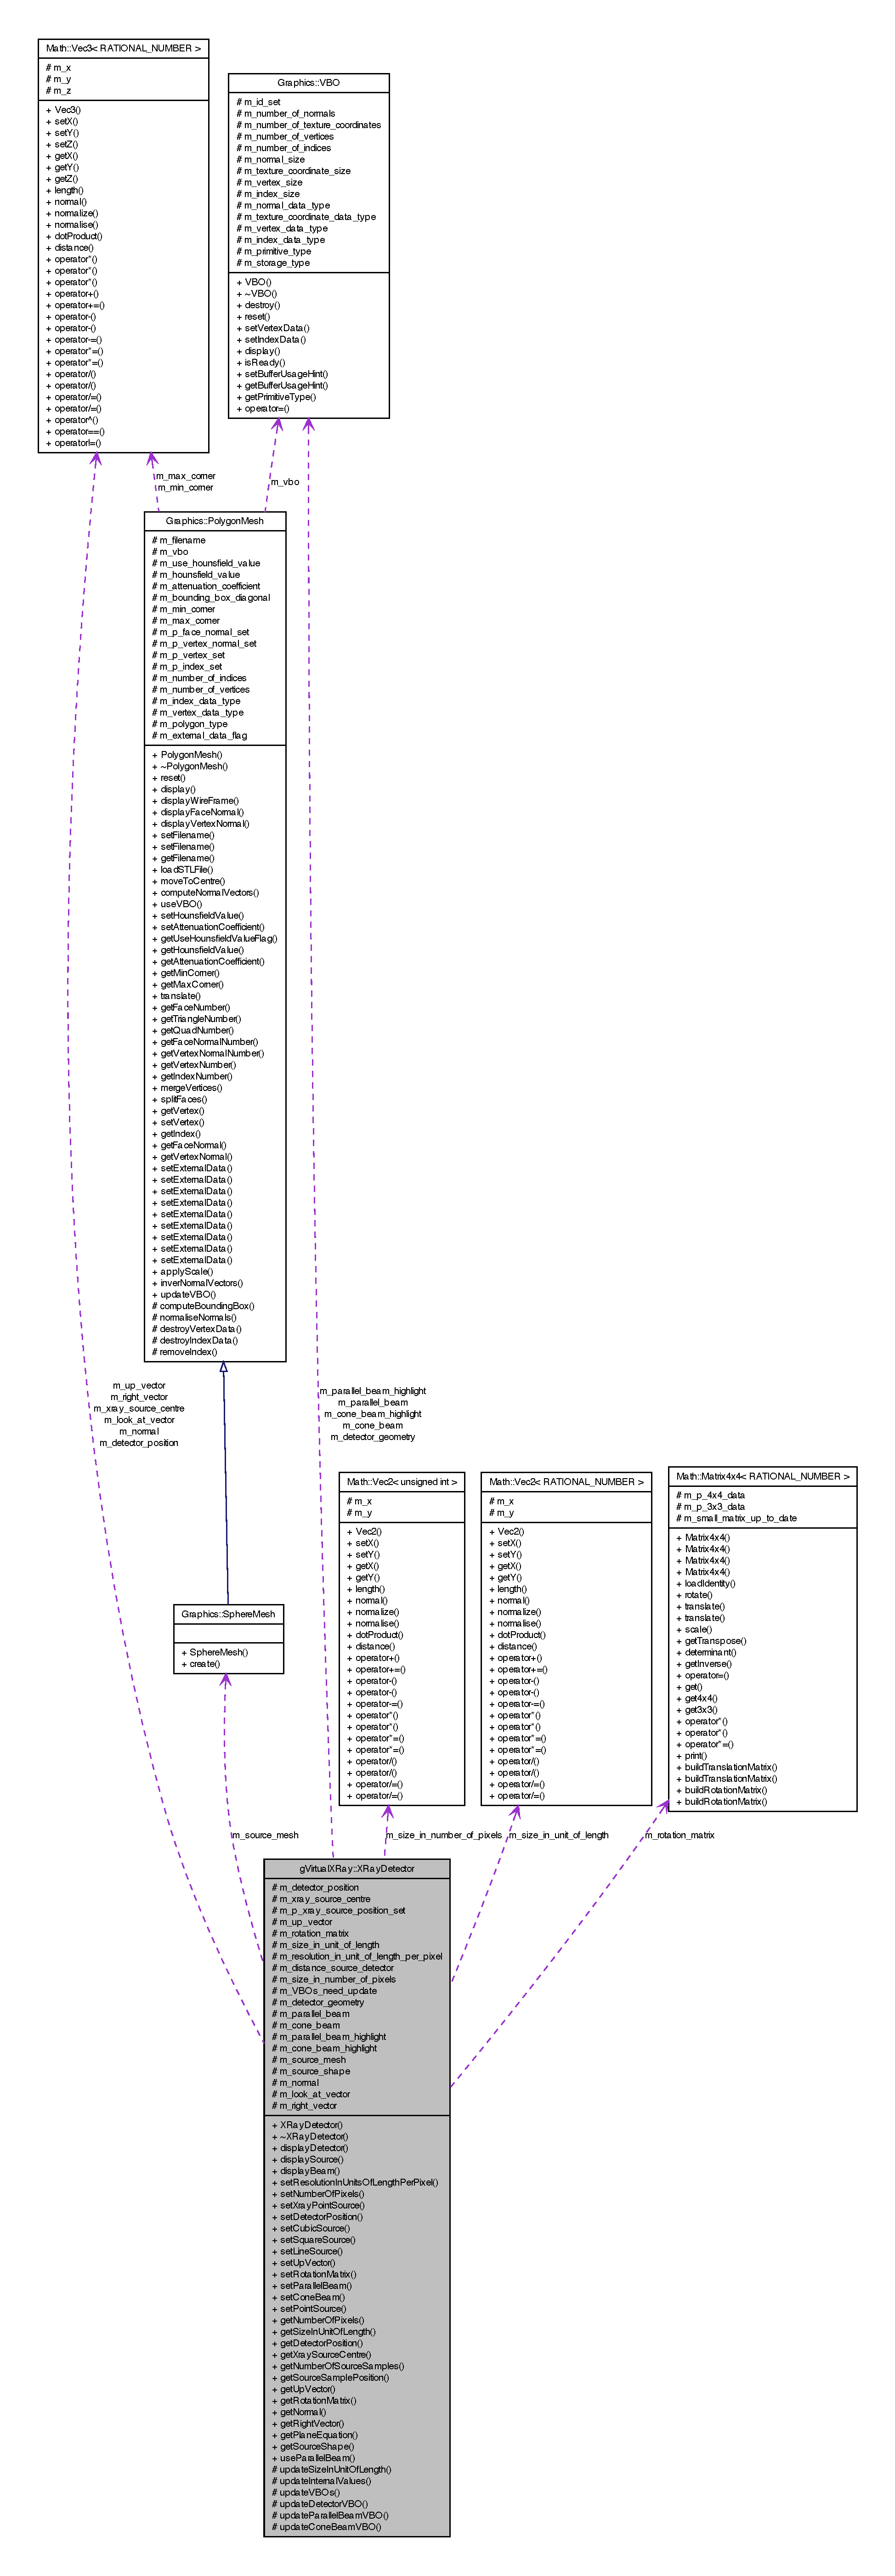
\includegraphics[height=600pt]{classg_virtual_x_ray_1_1_x_ray_detector__coll__graph}
\end{center}
\end{figure}
\subsection*{Public Types}
\begin{DoxyCompactItemize}
\item 
enum \hyperlink{classg_virtual_x_ray_1_1_x_ray_detector_af449ad932589ae761d9da74e4c211c79}{SourceShapeTag} \{ \par
\hyperlink{classg_virtual_x_ray_1_1_x_ray_detector_af449ad932589ae761d9da74e4c211c79a4882661dba7e23a6ff7110402da42ca8}{POINT}, 
\hyperlink{classg_virtual_x_ray_1_1_x_ray_detector_af449ad932589ae761d9da74e4c211c79ae13714fe3186a696083deb3e1e33c0ba}{SQUARE}, 
\hyperlink{classg_virtual_x_ray_1_1_x_ray_detector_af449ad932589ae761d9da74e4c211c79abd057f7d5135ab26e5eb454f09f8779a}{CUBE}, 
\hyperlink{classg_virtual_x_ray_1_1_x_ray_detector_af449ad932589ae761d9da74e4c211c79a18991f3a7905cf4901e17a1c47e78baa}{LINE}, 
\par
\hyperlink{classg_virtual_x_ray_1_1_x_ray_detector_af449ad932589ae761d9da74e4c211c79abd2cf25b675efca5ea2ec87b758857e5}{PARALLEL}, 
\hyperlink{classg_virtual_x_ray_1_1_x_ray_detector_af449ad932589ae761d9da74e4c211c79aaaf70d790c006bd643da4394550c678b}{UNKNOWN\_\-SHAPE}
 \}
\begin{DoxyCompactList}\small\item\em SourceShape is a type that defines the shape of X-\/ray sources. \end{DoxyCompactList}\item 
typedef enum \hyperlink{classg_virtual_x_ray_1_1_x_ray_detector_af449ad932589ae761d9da74e4c211c79}{gVirtualXRay::XRayDetector::SourceShapeTag} \hyperlink{classg_virtual_x_ray_1_1_x_ray_detector_a217628a4ed1ca8ed8031b288fb09d335}{SourceShape}
\begin{DoxyCompactList}\small\item\em SourceShape is a type that defines the shape of X-\/ray sources. \end{DoxyCompactList}\end{DoxyCompactItemize}
\subsection*{Public Member Functions}
\begin{DoxyCompactItemize}
\item 
\hyperlink{classg_virtual_x_ray_1_1_x_ray_detector_aa711b947ac963941891c1f8c61cc7ff8}{XRayDetector} ()
\begin{DoxyCompactList}\small\item\em Default constructor. \end{DoxyCompactList}\item 
\hyperlink{classg_virtual_x_ray_1_1_x_ray_detector_afcfac202d93f170ff1d8c8e92849ab3e}{$\sim$XRayDetector} ()
\begin{DoxyCompactList}\small\item\em Destructor. \end{DoxyCompactList}\item 
void \hyperlink{classg_virtual_x_ray_1_1_x_ray_detector_a0b33600bfa074ac167ea604ba38f664c}{displayDetector} ()
\begin{DoxyCompactList}\small\item\em Display the detector using OpenGL. \end{DoxyCompactList}\item 
void \hyperlink{classg_virtual_x_ray_1_1_x_ray_detector_a378f40f0e8d3a7798488f1ed21d44694}{displaySource} ()
\begin{DoxyCompactList}\small\item\em Display the source using OpenGL. \end{DoxyCompactList}\item 
void \hyperlink{classg_virtual_x_ray_1_1_x_ray_detector_aed46b4bae356dfdcfa5e73382f6fb4c5}{displayBeam} ()
\begin{DoxyCompactList}\small\item\em Display the beam using OpenGL. \end{DoxyCompactList}\item 
void \hyperlink{classg_virtual_x_ray_1_1_x_ray_detector_ab542086c90a3d96e45ebe8d965c25938}{setResolutionInUnitsOfLengthPerPixel} (const \hyperlink{namespace_utilities_a40969b96bd8d847b962e297cb79f08ce}{RATIONAL\_\-NUMBER} \&aResolution)
\item 
void \hyperlink{classg_virtual_x_ray_1_1_x_ray_detector_a6ed821d0fc9c41184d8745f5615caae0}{setNumberOfPixels} (const \hyperlink{class_math_1_1_vec2}{Vec2ui} \&aSizeInPixels)
\begin{DoxyCompactList}\small\item\em Set the number of pixels. \end{DoxyCompactList}\item 
void \hyperlink{classg_virtual_x_ray_1_1_x_ray_detector_a643cbb35e442638652c828710d722900}{setXrayPointSource} (const \hyperlink{class_math_1_1_vec3}{VEC3} \&aXraySourcePosition)
\begin{DoxyCompactList}\small\item\em Set the position of the X-\/ray source. \end{DoxyCompactList}\item 
void \hyperlink{classg_virtual_x_ray_1_1_x_ray_detector_a4eed3c71235a854b66fd5212316d3a73}{setDetectorPosition} (const \hyperlink{class_math_1_1_vec3}{VEC3} \&aDetectorPosition)
\begin{DoxyCompactList}\small\item\em Set the position of the X-\/ray detector. \end{DoxyCompactList}\item 
void \hyperlink{classg_virtual_x_ray_1_1_x_ray_detector_a346c280ce7648e4fcc7f42bbb06e6ab7}{setCubicSource} (const \hyperlink{class_math_1_1_vec3}{VEC3} \&aXraySourcePosition, unsigned int aNumberOfSamplesAlongOneDirection, \hyperlink{namespace_utilities_a40969b96bd8d847b962e297cb79f08ce}{RATIONAL\_\-NUMBER} aLength)
\begin{DoxyCompactList}\small\item\em Set the shape of the source as a cube. \end{DoxyCompactList}\item 
void \hyperlink{classg_virtual_x_ray_1_1_x_ray_detector_aa6f970bda1aa9ba777f6b4cc99102ea3}{setSquareSource} (const \hyperlink{class_math_1_1_vec3}{VEC3} \&aXraySourcePosition, unsigned int aNumberOfSamplesAlongOneDirection, \hyperlink{namespace_utilities_a40969b96bd8d847b962e297cb79f08ce}{RATIONAL\_\-NUMBER} aLength)
\begin{DoxyCompactList}\small\item\em Set the shape of the source as a square. \end{DoxyCompactList}\item 
void \hyperlink{classg_virtual_x_ray_1_1_x_ray_detector_a5bbcd6912a95907c1f4268f065146690}{setLineSource} (const \hyperlink{class_math_1_1_vec3}{VEC3} \&aXraySourcePosition, const \hyperlink{class_math_1_1_vec3}{VEC3} \&aDirection, unsigned int aNumberOfSamplesAlongOneDirection, \hyperlink{namespace_utilities_a40969b96bd8d847b962e297cb79f08ce}{RATIONAL\_\-NUMBER} aLength)
\begin{DoxyCompactList}\small\item\em Set the shape of the source as a line segment. \end{DoxyCompactList}\item 
void \hyperlink{classg_virtual_x_ray_1_1_x_ray_detector_aa314d10cf703d9bdeb990cfb48dd8b98}{setUpVector} (const \hyperlink{class_math_1_1_vec3}{VEC3} \&anUpVector)
\begin{DoxyCompactList}\small\item\em Set the up vector that defines the detector's orientation. \end{DoxyCompactList}\item 
void \hyperlink{classg_virtual_x_ray_1_1_x_ray_detector_a8ee8fd3a51eb1f69b17d8d3f9cf6abf5}{setRotationMatrix} (const \hyperlink{class_math_1_1_matrix4x4}{MATRIX4} \&aMatrix)
\begin{DoxyCompactList}\small\item\em Set the rotation matrix. \end{DoxyCompactList}\item 
void \hyperlink{classg_virtual_x_ray_1_1_x_ray_detector_a057d66f5441834356cfe12eec8a07f3f}{setParallelBeam} ()
\begin{DoxyCompactList}\small\item\em Set the projection mode to parallel beam. \end{DoxyCompactList}\item 
void \hyperlink{classg_virtual_x_ray_1_1_x_ray_detector_aa14a5b6d79649f4f9dd02aa502cee45a}{setConeBeam} ()
\begin{DoxyCompactList}\small\item\em Set the projection mode to cone beam (same as point source). \end{DoxyCompactList}\item 
void \hyperlink{classg_virtual_x_ray_1_1_x_ray_detector_a815ce2cb19adb38f11a9e2572aa9095c}{setPointSource} ()
\begin{DoxyCompactList}\small\item\em Set the projection mode to point source (same as cone beam). \end{DoxyCompactList}\item 
const \hyperlink{class_math_1_1_vec2}{Vec2ui} \& \hyperlink{classg_virtual_x_ray_1_1_x_ray_detector_a159d091558da004b17a4d5cccea0e672}{getNumberOfPixels} () const 
\begin{DoxyCompactList}\small\item\em Accessor on the number of pixels. \end{DoxyCompactList}\item 
const \hyperlink{class_math_1_1_vec2}{VEC2} \& \hyperlink{classg_virtual_x_ray_1_1_x_ray_detector_ab1889277924050412fdddc6716e5bc0c}{getSizeInUnitOfLength} () const 
\begin{DoxyCompactList}\small\item\em Accessor on the size of the detector (in unit of length). \end{DoxyCompactList}\item 
const \hyperlink{class_math_1_1_vec3}{VEC3} \& \hyperlink{classg_virtual_x_ray_1_1_x_ray_detector_a602b3799826827286d9fa9a155c4f33b}{getDetectorPosition} () const 
\begin{DoxyCompactList}\small\item\em Accessor on the detector position. \end{DoxyCompactList}\item 
const \hyperlink{class_math_1_1_vec3}{VEC3} \& \hyperlink{classg_virtual_x_ray_1_1_x_ray_detector_a04653d1dbe55f256889fe90207a46cf7}{getXraySourceCentre} () const 
\begin{DoxyCompactList}\small\item\em Accessor on the centre of the source. \end{DoxyCompactList}\item 
unsigned int \hyperlink{classg_virtual_x_ray_1_1_x_ray_detector_a518e95dda16004376bfdc624ff3495e0}{getNumberOfSourceSamples} () const 
\item 
const \hyperlink{class_math_1_1_vec3}{VEC3} \& \hyperlink{classg_virtual_x_ray_1_1_x_ray_detector_ae041d6539cd7b225dc224401d4d3a209}{getSourceSamplePosition} (unsigned int aSampleID) const 
\item 
const \hyperlink{class_math_1_1_vec3}{VEC3} \& \hyperlink{classg_virtual_x_ray_1_1_x_ray_detector_a355b93b5a269841c03aa4ef8c5786f92}{getUpVector} () const 
\begin{DoxyCompactList}\small\item\em Accessor on the up vector, which defines the orientation of the detector. \end{DoxyCompactList}\item 
const \hyperlink{class_math_1_1_matrix4x4}{MATRIX4} \& \hyperlink{classg_virtual_x_ray_1_1_x_ray_detector_aac6ab2cb0ea5c20211d0783bd6a8cfcc}{getRotationMatrix} () const 
\begin{DoxyCompactList}\small\item\em Accessor on the rotation matrix. \end{DoxyCompactList}\item 
const \hyperlink{class_math_1_1_vec3}{VEC3} \& \hyperlink{classg_virtual_x_ray_1_1_x_ray_detector_adfa24796ba538502309367546c0aca48}{getNormal} () const 
\begin{DoxyCompactList}\small\item\em Accessor on the vector normal to the detector. \end{DoxyCompactList}\item 
const \hyperlink{class_math_1_1_vec3}{VEC3} \& \hyperlink{classg_virtual_x_ray_1_1_x_ray_detector_ad0d1e7a338d175c1194c7be9c15f5453}{getRightVector} () const 
\begin{DoxyCompactList}\small\item\em Accessor on the cross product between m\_\-look\_\-at\_\-vector and m\_\-up\_\-vector. \end{DoxyCompactList}\item 
const void \hyperlink{classg_virtual_x_ray_1_1_x_ray_detector_abd408fcf45d19386de9c0ef749b9d66e}{getPlaneEquation} (\hyperlink{namespace_utilities_a40969b96bd8d847b962e297cb79f08ce}{RATIONAL\_\-NUMBER} \&A, \hyperlink{namespace_utilities_a40969b96bd8d847b962e297cb79f08ce}{RATIONAL\_\-NUMBER} \&B, \hyperlink{namespace_utilities_a40969b96bd8d847b962e297cb79f08ce}{RATIONAL\_\-NUMBER} \&C, \hyperlink{namespace_utilities_a40969b96bd8d847b962e297cb79f08ce}{RATIONAL\_\-NUMBER} \&D)
\begin{DoxyCompactList}\small\item\em Accessor on the plane equation (Ax + By + Cz + D = 0). \end{DoxyCompactList}\item 
\hyperlink{classg_virtual_x_ray_1_1_x_ray_detector_a217628a4ed1ca8ed8031b288fb09d335}{SourceShape} \hyperlink{classg_virtual_x_ray_1_1_x_ray_detector_a8d9cd9cbe4dde868a076a1ec1aa30716}{getSourceShape} () const 
\begin{DoxyCompactList}\small\item\em Accessor on the shape of the source. \end{DoxyCompactList}\item 
bool \hyperlink{classg_virtual_x_ray_1_1_x_ray_detector_a00d1e230285e636afdb7a0321f2514de}{useParallelBeam} () const 
\begin{DoxyCompactList}\small\item\em Accessor on the flag about projection. \end{DoxyCompactList}\end{DoxyCompactItemize}
\subsection*{Protected Member Functions}
\begin{DoxyCompactItemize}
\item 
void \hyperlink{classg_virtual_x_ray_1_1_x_ray_detector_a0af3ef3845b74a97c343b104b4b8b3de}{updateSizeInUnitOfLength} ()
\begin{DoxyCompactList}\small\item\em Compute the size of the detector. \end{DoxyCompactList}\item 
void \hyperlink{classg_virtual_x_ray_1_1_x_ray_detector_a5e1c0c7e3bc3de8d7b53fb7a39449531}{updateInternalValues} ()
\begin{DoxyCompactList}\small\item\em Compute the distance between the source and the detector, etc. \end{DoxyCompactList}\item 
void \hyperlink{classg_virtual_x_ray_1_1_x_ray_detector_a80b7e44aebf23505d0bbefb5001eb42b}{updateVBOs} ()
\begin{DoxyCompactList}\small\item\em Update the VBOs. \end{DoxyCompactList}\item 
void \hyperlink{classg_virtual_x_ray_1_1_x_ray_detector_a8b88ed5684d2baa3434cb6435fe60307}{updateDetectorVBO} ()
\begin{DoxyCompactList}\small\item\em Update the VBO of the detector. \end{DoxyCompactList}\item 
void \hyperlink{classg_virtual_x_ray_1_1_x_ray_detector_a9680618cf54382c498233104faede526}{updateParallelBeamVBO} ()
\begin{DoxyCompactList}\small\item\em Update the VBO of the parallel beam. \end{DoxyCompactList}\item 
void \hyperlink{classg_virtual_x_ray_1_1_x_ray_detector_a672cdc396edb08fac9e33a95d17baa7d}{updateConeBeamVBO} ()
\begin{DoxyCompactList}\small\item\em Update the VBO of the cone beam. \end{DoxyCompactList}\end{DoxyCompactItemize}
\subsection*{Protected Attributes}
\begin{DoxyCompactItemize}
\item 
\hyperlink{class_math_1_1_vec3}{VEC3} \hyperlink{classg_virtual_x_ray_1_1_x_ray_detector_af60ca47a7687066d3c474146a4a9f85a}{m\_\-detector\_\-position}
\begin{DoxyCompactList}\small\item\em The position of the detector centre. \end{DoxyCompactList}\item 
\hyperlink{class_math_1_1_vec3}{VEC3} \hyperlink{classg_virtual_x_ray_1_1_x_ray_detector_abc32b66cca7b4e14d3ddce4fcd31c497}{m\_\-xray\_\-source\_\-centre}
\begin{DoxyCompactList}\small\item\em The position of the source centre. \end{DoxyCompactList}\item 
std::vector$<$ \hyperlink{class_math_1_1_vec3}{VEC3} $>$ \hyperlink{classg_virtual_x_ray_1_1_x_ray_detector_a2669db81b788d9bf9e3f91ffc7a385d5}{m\_\-p\_\-xray\_\-source\_\-position\_\-set}
\begin{DoxyCompactList}\small\item\em The sample positions of the source. \end{DoxyCompactList}\item 
\hyperlink{class_math_1_1_vec3}{VEC3} \hyperlink{classg_virtual_x_ray_1_1_x_ray_detector_ac03caffd75f0386f2dda388c2c38b782}{m\_\-up\_\-vector}
\begin{DoxyCompactList}\small\item\em The \char`\"{}up\char`\"{} vector the the detector. \end{DoxyCompactList}\item 
\hyperlink{class_math_1_1_matrix4x4}{MATRIX4} \hyperlink{classg_virtual_x_ray_1_1_x_ray_detector_a939ddb2d6fb51e831236ee0ccffc7ec8}{m\_\-rotation\_\-matrix}
\begin{DoxyCompactList}\small\item\em The rotation matrix. \end{DoxyCompactList}\item 
\hyperlink{class_math_1_1_vec2}{VEC2} \hyperlink{classg_virtual_x_ray_1_1_x_ray_detector_a742613089e3a523792c5b253020d7d98}{m\_\-size\_\-in\_\-unit\_\-of\_\-length}
\begin{DoxyCompactList}\small\item\em The size of the detector. \end{DoxyCompactList}\item 
\hyperlink{namespace_utilities_a40969b96bd8d847b962e297cb79f08ce}{RATIONAL\_\-NUMBER} \hyperlink{classg_virtual_x_ray_1_1_x_ray_detector_a437004cdae0f0b03840c0dce2a0018d0}{m\_\-resolution\_\-in\_\-unit\_\-of\_\-length\_\-per\_\-pixel}
\begin{DoxyCompactList}\small\item\em Resolution (in unit of length per pixel) \end{DoxyCompactList}\item 
\hyperlink{namespace_utilities_a40969b96bd8d847b962e297cb79f08ce}{RATIONAL\_\-NUMBER} \hyperlink{classg_virtual_x_ray_1_1_x_ray_detector_a3b6ebd87b12d0fb434671309d252a00c}{m\_\-distance\_\-source\_\-detector}
\begin{DoxyCompactList}\small\item\em Distance between the source and the detector. \end{DoxyCompactList}\item 
\hyperlink{class_math_1_1_vec2}{Vec2ui} \hyperlink{classg_virtual_x_ray_1_1_x_ray_detector_a07c8671a6c02fb8b99e4b7c5d23cb8cf}{m\_\-size\_\-in\_\-number\_\-of\_\-pixels}
\begin{DoxyCompactList}\small\item\em Size of the detector (in number of pixels) \end{DoxyCompactList}\item 
bool \hyperlink{classg_virtual_x_ray_1_1_x_ray_detector_a69d92de8630dfb70270b914a4b3459a9}{m\_\-VBOs\_\-need\_\-update}
\begin{DoxyCompactList}\small\item\em A flag set to true when the VBOs need to be updated. \end{DoxyCompactList}\item 
\hyperlink{class_graphics_1_1_v_b_o}{VBO} \hyperlink{classg_virtual_x_ray_1_1_x_ray_detector_a2090842d641ea37cc03fd7da384c8c67}{m\_\-detector\_\-geometry}
\begin{DoxyCompactList}\small\item\em The triangle mesh corresponding to the detector. \end{DoxyCompactList}\item 
\hyperlink{class_graphics_1_1_v_b_o}{VBO} \hyperlink{classg_virtual_x_ray_1_1_x_ray_detector_af532ddbb920e88e98976704e56a103bb}{m\_\-parallel\_\-beam}
\begin{DoxyCompactList}\small\item\em The triangle mesh corresponding to the parallel beam. \end{DoxyCompactList}\item 
\hyperlink{class_graphics_1_1_v_b_o}{VBO} \hyperlink{classg_virtual_x_ray_1_1_x_ray_detector_a60e4ff579d75738cc9f91236b5dde9cc}{m\_\-cone\_\-beam}
\begin{DoxyCompactList}\small\item\em The triangle mesh corresponding to the cone beam. \end{DoxyCompactList}\item 
\hyperlink{class_graphics_1_1_v_b_o}{VBO} \hyperlink{classg_virtual_x_ray_1_1_x_ray_detector_a10c10c59b7b73a7b7ab2d78ee03520c9}{m\_\-parallel\_\-beam\_\-highlight}
\begin{DoxyCompactList}\small\item\em The triangle mesh corresponding to the parallel beam highlight. \end{DoxyCompactList}\item 
\hyperlink{class_graphics_1_1_v_b_o}{VBO} \hyperlink{classg_virtual_x_ray_1_1_x_ray_detector_a8b5bc9482b244b0b1fe309df2d4300e7}{m\_\-cone\_\-beam\_\-highlight}
\begin{DoxyCompactList}\small\item\em The triangle mesh corresponding to the cone beam highlight. \end{DoxyCompactList}\item 
\hyperlink{class_graphics_1_1_sphere_mesh}{SphereMesh} \hyperlink{classg_virtual_x_ray_1_1_x_ray_detector_a3c61d804f04b81a2aeab9afa09a2644d}{m\_\-source\_\-mesh}
\begin{DoxyCompactList}\small\item\em Polygon mesh of the source. \end{DoxyCompactList}\item 
\hyperlink{classg_virtual_x_ray_1_1_x_ray_detector_a217628a4ed1ca8ed8031b288fb09d335}{SourceShape} \hyperlink{classg_virtual_x_ray_1_1_x_ray_detector_a58ee142a64962d69bb203fcae40a8c6f}{m\_\-source\_\-shape}
\begin{DoxyCompactList}\small\item\em Source type. \end{DoxyCompactList}\item 
\hyperlink{class_math_1_1_vec3}{VEC3} \hyperlink{classg_virtual_x_ray_1_1_x_ray_detector_a4e6928c0c2347c9371f320c72d334411}{m\_\-normal}
\begin{DoxyCompactList}\small\item\em The vector normal to the detector. \end{DoxyCompactList}\item 
\hyperlink{class_math_1_1_vec3}{VEC3} \hyperlink{classg_virtual_x_ray_1_1_x_ray_detector_a68163c9f1a543baef07c24388476b85f}{m\_\-look\_\-at\_\-vector}
\begin{DoxyCompactList}\small\item\em The viewing direction (i.e. the unit vector from the X-\/ray source to the centre of the detector) \end{DoxyCompactList}\item 
\hyperlink{class_math_1_1_vec3}{VEC3} \hyperlink{classg_virtual_x_ray_1_1_x_ray_detector_a43c90e61c73da70e02f73929873b443c}{m\_\-right\_\-vector}
\begin{DoxyCompactList}\small\item\em The cross product between m\_\-look\_\-at\_\-vector and m\_\-up\_\-vector. \end{DoxyCompactList}\end{DoxyCompactItemize}


\subsection{Detailed Description}
\hyperlink{classg_virtual_x_ray_1_1_x_ray_detector}{XRayDetector} is a class to handle a X-\/ray detector. 

Definition at line 74 of file XRayDetector.h.



\subsection{Member Typedef Documentation}
\hypertarget{classg_virtual_x_ray_1_1_x_ray_detector_a217628a4ed1ca8ed8031b288fb09d335}{
\index{gVirtualXRay::XRayDetector@{gVirtualXRay::XRayDetector}!SourceShape@{SourceShape}}
\index{SourceShape@{SourceShape}!gVirtualXRay::XRayDetector@{gVirtualXRay::XRayDetector}}
\subsubsection[{SourceShape}]{\setlength{\rightskip}{0pt plus 5cm}typedef enum {\bf gVirtualXRay::XRayDetector::SourceShapeTag}  {\bf gVirtualXRay::XRayDetector::SourceShape}}}
\label{classg_virtual_x_ray_1_1_x_ray_detector_a217628a4ed1ca8ed8031b288fb09d335}


SourceShape is a type that defines the shape of X-\/ray sources. 



\subsection{Member Enumeration Documentation}
\hypertarget{classg_virtual_x_ray_1_1_x_ray_detector_af449ad932589ae761d9da74e4c211c79}{
\index{gVirtualXRay::XRayDetector@{gVirtualXRay::XRayDetector}!SourceShapeTag@{SourceShapeTag}}
\index{SourceShapeTag@{SourceShapeTag}!gVirtualXRay::XRayDetector@{gVirtualXRay::XRayDetector}}
\subsubsection[{SourceShapeTag}]{\setlength{\rightskip}{0pt plus 5cm}enum {\bf gVirtualXRay::XRayDetector::SourceShapeTag}}}
\label{classg_virtual_x_ray_1_1_x_ray_detector_af449ad932589ae761d9da74e4c211c79}


SourceShape is a type that defines the shape of X-\/ray sources. 

\begin{Desc}
\item[Enumerator: ]\par
\begin{description}
\index{POINT@{POINT}!gVirtualXRay::XRayDetector@{gVirtualXRay::XRayDetector}}\index{gVirtualXRay::XRayDetector@{gVirtualXRay::XRayDetector}!POINT@{POINT}}\item[{\em 
\hypertarget{classg_virtual_x_ray_1_1_x_ray_detector_af449ad932589ae761d9da74e4c211c79a4882661dba7e23a6ff7110402da42ca8}{
POINT}
\label{classg_virtual_x_ray_1_1_x_ray_detector_af449ad932589ae761d9da74e4c211c79a4882661dba7e23a6ff7110402da42ca8}
}]Infinitively small point source. \index{SQUARE@{SQUARE}!gVirtualXRay::XRayDetector@{gVirtualXRay::XRayDetector}}\index{gVirtualXRay::XRayDetector@{gVirtualXRay::XRayDetector}!SQUARE@{SQUARE}}\item[{\em 
\hypertarget{classg_virtual_x_ray_1_1_x_ray_detector_af449ad932589ae761d9da74e4c211c79ae13714fe3186a696083deb3e1e33c0ba}{
SQUARE}
\label{classg_virtual_x_ray_1_1_x_ray_detector_af449ad932589ae761d9da74e4c211c79ae13714fe3186a696083deb3e1e33c0ba}
}]Source whose shape corresponds to a square. \index{CUBE@{CUBE}!gVirtualXRay::XRayDetector@{gVirtualXRay::XRayDetector}}\index{gVirtualXRay::XRayDetector@{gVirtualXRay::XRayDetector}!CUBE@{CUBE}}\item[{\em 
\hypertarget{classg_virtual_x_ray_1_1_x_ray_detector_af449ad932589ae761d9da74e4c211c79abd057f7d5135ab26e5eb454f09f8779a}{
CUBE}
\label{classg_virtual_x_ray_1_1_x_ray_detector_af449ad932589ae761d9da74e4c211c79abd057f7d5135ab26e5eb454f09f8779a}
}]Source whose shape corresponds to a cube. \index{LINE@{LINE}!gVirtualXRay::XRayDetector@{gVirtualXRay::XRayDetector}}\index{gVirtualXRay::XRayDetector@{gVirtualXRay::XRayDetector}!LINE@{LINE}}\item[{\em 
\hypertarget{classg_virtual_x_ray_1_1_x_ray_detector_af449ad932589ae761d9da74e4c211c79a18991f3a7905cf4901e17a1c47e78baa}{
LINE}
\label{classg_virtual_x_ray_1_1_x_ray_detector_af449ad932589ae761d9da74e4c211c79a18991f3a7905cf4901e17a1c47e78baa}
}]Source whose shape corresponds to a line segment. \index{PARALLEL@{PARALLEL}!gVirtualXRay::XRayDetector@{gVirtualXRay::XRayDetector}}\index{gVirtualXRay::XRayDetector@{gVirtualXRay::XRayDetector}!PARALLEL@{PARALLEL}}\item[{\em 
\hypertarget{classg_virtual_x_ray_1_1_x_ray_detector_af449ad932589ae761d9da74e4c211c79abd2cf25b675efca5ea2ec87b758857e5}{
PARALLEL}
\label{classg_virtual_x_ray_1_1_x_ray_detector_af449ad932589ae761d9da74e4c211c79abd2cf25b675efca5ea2ec87b758857e5}
}]Parallel source, i.e. a point source infinitely far away. \index{UNKNOWN\_\-SHAPE@{UNKNOWN\_\-SHAPE}!gVirtualXRay::XRayDetector@{gVirtualXRay::XRayDetector}}\index{gVirtualXRay::XRayDetector@{gVirtualXRay::XRayDetector}!UNKNOWN\_\-SHAPE@{UNKNOWN\_\-SHAPE}}\item[{\em 
\hypertarget{classg_virtual_x_ray_1_1_x_ray_detector_af449ad932589ae761d9da74e4c211c79aaaf70d790c006bd643da4394550c678b}{
UNKNOWN\_\-SHAPE}
\label{classg_virtual_x_ray_1_1_x_ray_detector_af449ad932589ae761d9da74e4c211c79aaaf70d790c006bd643da4394550c678b}
}]Unknown type. \end{description}
\end{Desc}



Definition at line 80 of file XRayDetector.h.



\subsection{Constructor \& Destructor Documentation}
\hypertarget{classg_virtual_x_ray_1_1_x_ray_detector_aa711b947ac963941891c1f8c61cc7ff8}{
\index{gVirtualXRay::XRayDetector@{gVirtualXRay::XRayDetector}!XRayDetector@{XRayDetector}}
\index{XRayDetector@{XRayDetector}!gVirtualXRay::XRayDetector@{gVirtualXRay::XRayDetector}}
\subsubsection[{XRayDetector}]{\setlength{\rightskip}{0pt plus 5cm}gVirtualXRay::XRayDetector::XRayDetector (
\begin{DoxyParamCaption}
{}
\end{DoxyParamCaption}
)\hspace{0.3cm}{\ttfamily  \mbox{[}inline\mbox{]}}}}
\label{classg_virtual_x_ray_1_1_x_ray_detector_aa711b947ac963941891c1f8c61cc7ff8}


Default constructor. 



Definition at line 47 of file XRayDetector.inl.

\hypertarget{classg_virtual_x_ray_1_1_x_ray_detector_afcfac202d93f170ff1d8c8e92849ab3e}{
\index{gVirtualXRay::XRayDetector@{gVirtualXRay::XRayDetector}!$\sim$XRayDetector@{$\sim$XRayDetector}}
\index{$\sim$XRayDetector@{$\sim$XRayDetector}!gVirtualXRay::XRayDetector@{gVirtualXRay::XRayDetector}}
\subsubsection[{$\sim$XRayDetector}]{\setlength{\rightskip}{0pt plus 5cm}gVirtualXRay::XRayDetector::$\sim$XRayDetector (
\begin{DoxyParamCaption}
{}
\end{DoxyParamCaption}
)\hspace{0.3cm}{\ttfamily  \mbox{[}inline\mbox{]}}}}
\label{classg_virtual_x_ray_1_1_x_ray_detector_afcfac202d93f170ff1d8c8e92849ab3e}


Destructor. 



Definition at line 60 of file XRayDetector.inl.



\subsection{Member Function Documentation}
\hypertarget{classg_virtual_x_ray_1_1_x_ray_detector_aed46b4bae356dfdcfa5e73382f6fb4c5}{
\index{gVirtualXRay::XRayDetector@{gVirtualXRay::XRayDetector}!displayBeam@{displayBeam}}
\index{displayBeam@{displayBeam}!gVirtualXRay::XRayDetector@{gVirtualXRay::XRayDetector}}
\subsubsection[{displayBeam}]{\setlength{\rightskip}{0pt plus 5cm}void gVirtualXRay::XRayDetector::displayBeam (
\begin{DoxyParamCaption}
{}
\end{DoxyParamCaption}
)}}
\label{classg_virtual_x_ray_1_1_x_ray_detector_aed46b4bae356dfdcfa5e73382f6fb4c5}


Display the beam using OpenGL. 

\hypertarget{classg_virtual_x_ray_1_1_x_ray_detector_a0b33600bfa074ac167ea604ba38f664c}{
\index{gVirtualXRay::XRayDetector@{gVirtualXRay::XRayDetector}!displayDetector@{displayDetector}}
\index{displayDetector@{displayDetector}!gVirtualXRay::XRayDetector@{gVirtualXRay::XRayDetector}}
\subsubsection[{displayDetector}]{\setlength{\rightskip}{0pt plus 5cm}void gVirtualXRay::XRayDetector::displayDetector (
\begin{DoxyParamCaption}
{}
\end{DoxyParamCaption}
)}}
\label{classg_virtual_x_ray_1_1_x_ray_detector_a0b33600bfa074ac167ea604ba38f664c}


Display the detector using OpenGL. 

\hypertarget{classg_virtual_x_ray_1_1_x_ray_detector_a378f40f0e8d3a7798488f1ed21d44694}{
\index{gVirtualXRay::XRayDetector@{gVirtualXRay::XRayDetector}!displaySource@{displaySource}}
\index{displaySource@{displaySource}!gVirtualXRay::XRayDetector@{gVirtualXRay::XRayDetector}}
\subsubsection[{displaySource}]{\setlength{\rightskip}{0pt plus 5cm}void gVirtualXRay::XRayDetector::displaySource (
\begin{DoxyParamCaption}
{}
\end{DoxyParamCaption}
)\hspace{0.3cm}{\ttfamily  \mbox{[}inline\mbox{]}}}}
\label{classg_virtual_x_ray_1_1_x_ray_detector_a378f40f0e8d3a7798488f1ed21d44694}


Display the source using OpenGL. 



Definition at line 67 of file XRayDetector.inl.

\hypertarget{classg_virtual_x_ray_1_1_x_ray_detector_a602b3799826827286d9fa9a155c4f33b}{
\index{gVirtualXRay::XRayDetector@{gVirtualXRay::XRayDetector}!getDetectorPosition@{getDetectorPosition}}
\index{getDetectorPosition@{getDetectorPosition}!gVirtualXRay::XRayDetector@{gVirtualXRay::XRayDetector}}
\subsubsection[{getDetectorPosition}]{\setlength{\rightskip}{0pt plus 5cm}const {\bf VEC3} \& gVirtualXRay::XRayDetector::getDetectorPosition (
\begin{DoxyParamCaption}
{}
\end{DoxyParamCaption}
) const\hspace{0.3cm}{\ttfamily  \mbox{[}inline\mbox{]}}}}
\label{classg_virtual_x_ray_1_1_x_ray_detector_a602b3799826827286d9fa9a155c4f33b}


Accessor on the detector position. 

\begin{DoxyReturn}{Returns}
the detector position 
\end{DoxyReturn}


Definition at line 236 of file XRayDetector.inl.

\hypertarget{classg_virtual_x_ray_1_1_x_ray_detector_adfa24796ba538502309367546c0aca48}{
\index{gVirtualXRay::XRayDetector@{gVirtualXRay::XRayDetector}!getNormal@{getNormal}}
\index{getNormal@{getNormal}!gVirtualXRay::XRayDetector@{gVirtualXRay::XRayDetector}}
\subsubsection[{getNormal}]{\setlength{\rightskip}{0pt plus 5cm}const {\bf VEC3}\& gVirtualXRay::XRayDetector::getNormal (
\begin{DoxyParamCaption}
{}
\end{DoxyParamCaption}
) const}}
\label{classg_virtual_x_ray_1_1_x_ray_detector_adfa24796ba538502309367546c0aca48}


Accessor on the vector normal to the detector. 

\hypertarget{classg_virtual_x_ray_1_1_x_ray_detector_a159d091558da004b17a4d5cccea0e672}{
\index{gVirtualXRay::XRayDetector@{gVirtualXRay::XRayDetector}!getNumberOfPixels@{getNumberOfPixels}}
\index{getNumberOfPixels@{getNumberOfPixels}!gVirtualXRay::XRayDetector@{gVirtualXRay::XRayDetector}}
\subsubsection[{getNumberOfPixels}]{\setlength{\rightskip}{0pt plus 5cm}const {\bf Vec2ui} \& gVirtualXRay::XRayDetector::getNumberOfPixels (
\begin{DoxyParamCaption}
{}
\end{DoxyParamCaption}
) const\hspace{0.3cm}{\ttfamily  \mbox{[}inline\mbox{]}}}}
\label{classg_virtual_x_ray_1_1_x_ray_detector_a159d091558da004b17a4d5cccea0e672}


Accessor on the number of pixels. 

\begin{DoxyReturn}{Returns}
the number of pixels 
\end{DoxyReturn}


Definition at line 220 of file XRayDetector.inl.

\hypertarget{classg_virtual_x_ray_1_1_x_ray_detector_a518e95dda16004376bfdc624ff3495e0}{
\index{gVirtualXRay::XRayDetector@{gVirtualXRay::XRayDetector}!getNumberOfSourceSamples@{getNumberOfSourceSamples}}
\index{getNumberOfSourceSamples@{getNumberOfSourceSamples}!gVirtualXRay::XRayDetector@{gVirtualXRay::XRayDetector}}
\subsubsection[{getNumberOfSourceSamples}]{\setlength{\rightskip}{0pt plus 5cm}unsigned int gVirtualXRay::XRayDetector::getNumberOfSourceSamples (
\begin{DoxyParamCaption}
{}
\end{DoxyParamCaption}
) const\hspace{0.3cm}{\ttfamily  \mbox{[}inline\mbox{]}}}}
\label{classg_virtual_x_ray_1_1_x_ray_detector_a518e95dda16004376bfdc624ff3495e0}


Definition at line 252 of file XRayDetector.inl.

\hypertarget{classg_virtual_x_ray_1_1_x_ray_detector_abd408fcf45d19386de9c0ef749b9d66e}{
\index{gVirtualXRay::XRayDetector@{gVirtualXRay::XRayDetector}!getPlaneEquation@{getPlaneEquation}}
\index{getPlaneEquation@{getPlaneEquation}!gVirtualXRay::XRayDetector@{gVirtualXRay::XRayDetector}}
\subsubsection[{getPlaneEquation}]{\setlength{\rightskip}{0pt plus 5cm}const void gVirtualXRay::XRayDetector::getPlaneEquation (
\begin{DoxyParamCaption}
\item[{{\bf RATIONAL\_\-NUMBER} \&}]{A, }
\item[{{\bf RATIONAL\_\-NUMBER} \&}]{B, }
\item[{{\bf RATIONAL\_\-NUMBER} \&}]{C, }
\item[{{\bf RATIONAL\_\-NUMBER} \&}]{D}
\end{DoxyParamCaption}
)\hspace{0.3cm}{\ttfamily  \mbox{[}inline\mbox{]}}}}
\label{classg_virtual_x_ray_1_1_x_ray_detector_abd408fcf45d19386de9c0ef749b9d66e}


Accessor on the plane equation (Ax + By + Cz + D = 0). 


\begin{DoxyParams}{Parameters}
{\em A,:} & the 1st component of the plane equation \\
\hline
{\em B,:} & the 2nd component of the plane equation \\
\hline
{\em C,:} & the 3rd component of the plane equation \\
\hline
{\em D,:} & the 4th component of the plane equation \\
\hline
\end{DoxyParams}


Definition at line 332 of file XRayDetector.inl.

\hypertarget{classg_virtual_x_ray_1_1_x_ray_detector_ad0d1e7a338d175c1194c7be9c15f5453}{
\index{gVirtualXRay::XRayDetector@{gVirtualXRay::XRayDetector}!getRightVector@{getRightVector}}
\index{getRightVector@{getRightVector}!gVirtualXRay::XRayDetector@{gVirtualXRay::XRayDetector}}
\subsubsection[{getRightVector}]{\setlength{\rightskip}{0pt plus 5cm}const {\bf VEC3} \& gVirtualXRay::XRayDetector::getRightVector (
\begin{DoxyParamCaption}
{}
\end{DoxyParamCaption}
) const\hspace{0.3cm}{\ttfamily  \mbox{[}inline\mbox{]}}}}
\label{classg_virtual_x_ray_1_1_x_ray_detector_ad0d1e7a338d175c1194c7be9c15f5453}


Accessor on the cross product between m\_\-look\_\-at\_\-vector and m\_\-up\_\-vector. 

\begin{DoxyReturn}{Returns}
the cross product 
\end{DoxyReturn}


Definition at line 276 of file XRayDetector.inl.

\hypertarget{classg_virtual_x_ray_1_1_x_ray_detector_aac6ab2cb0ea5c20211d0783bd6a8cfcc}{
\index{gVirtualXRay::XRayDetector@{gVirtualXRay::XRayDetector}!getRotationMatrix@{getRotationMatrix}}
\index{getRotationMatrix@{getRotationMatrix}!gVirtualXRay::XRayDetector@{gVirtualXRay::XRayDetector}}
\subsubsection[{getRotationMatrix}]{\setlength{\rightskip}{0pt plus 5cm}const {\bf MATRIX4} \& gVirtualXRay::XRayDetector::getRotationMatrix (
\begin{DoxyParamCaption}
{}
\end{DoxyParamCaption}
) const\hspace{0.3cm}{\ttfamily  \mbox{[}inline\mbox{]}}}}
\label{classg_virtual_x_ray_1_1_x_ray_detector_aac6ab2cb0ea5c20211d0783bd6a8cfcc}


Accessor on the rotation matrix. 

\begin{DoxyReturn}{Returns}
the rotation matrix 
\end{DoxyReturn}


Definition at line 284 of file XRayDetector.inl.

\hypertarget{classg_virtual_x_ray_1_1_x_ray_detector_ab1889277924050412fdddc6716e5bc0c}{
\index{gVirtualXRay::XRayDetector@{gVirtualXRay::XRayDetector}!getSizeInUnitOfLength@{getSizeInUnitOfLength}}
\index{getSizeInUnitOfLength@{getSizeInUnitOfLength}!gVirtualXRay::XRayDetector@{gVirtualXRay::XRayDetector}}
\subsubsection[{getSizeInUnitOfLength}]{\setlength{\rightskip}{0pt plus 5cm}const {\bf VEC2} \& gVirtualXRay::XRayDetector::getSizeInUnitOfLength (
\begin{DoxyParamCaption}
{}
\end{DoxyParamCaption}
) const\hspace{0.3cm}{\ttfamily  \mbox{[}inline\mbox{]}}}}
\label{classg_virtual_x_ray_1_1_x_ray_detector_ab1889277924050412fdddc6716e5bc0c}


Accessor on the size of the detector (in unit of length). 

\begin{DoxyReturn}{Returns}
the size of the detector 
\end{DoxyReturn}


Definition at line 228 of file XRayDetector.inl.

\hypertarget{classg_virtual_x_ray_1_1_x_ray_detector_ae041d6539cd7b225dc224401d4d3a209}{
\index{gVirtualXRay::XRayDetector@{gVirtualXRay::XRayDetector}!getSourceSamplePosition@{getSourceSamplePosition}}
\index{getSourceSamplePosition@{getSourceSamplePosition}!gVirtualXRay::XRayDetector@{gVirtualXRay::XRayDetector}}
\subsubsection[{getSourceSamplePosition}]{\setlength{\rightskip}{0pt plus 5cm}const {\bf VEC3} \& gVirtualXRay::XRayDetector::getSourceSamplePosition (
\begin{DoxyParamCaption}
\item[{unsigned int}]{aSampleID}
\end{DoxyParamCaption}
) const\hspace{0.3cm}{\ttfamily  \mbox{[}inline\mbox{]}}}}
\label{classg_virtual_x_ray_1_1_x_ray_detector_ae041d6539cd7b225dc224401d4d3a209}


Definition at line 260 of file XRayDetector.inl.

\hypertarget{classg_virtual_x_ray_1_1_x_ray_detector_a8d9cd9cbe4dde868a076a1ec1aa30716}{
\index{gVirtualXRay::XRayDetector@{gVirtualXRay::XRayDetector}!getSourceShape@{getSourceShape}}
\index{getSourceShape@{getSourceShape}!gVirtualXRay::XRayDetector@{gVirtualXRay::XRayDetector}}
\subsubsection[{getSourceShape}]{\setlength{\rightskip}{0pt plus 5cm}{\bf XRayDetector::SourceShape} gVirtualXRay::XRayDetector::getSourceShape (
\begin{DoxyParamCaption}
{}
\end{DoxyParamCaption}
) const\hspace{0.3cm}{\ttfamily  \mbox{[}inline\mbox{]}}}}
\label{classg_virtual_x_ray_1_1_x_ray_detector_a8d9cd9cbe4dde868a076a1ec1aa30716}


Accessor on the shape of the source. 

\begin{DoxyReturn}{Returns}
true if a parallel beam is used (e.g. orthographic projection), false if perspective projection is used 
\end{DoxyReturn}


Definition at line 292 of file XRayDetector.inl.

\hypertarget{classg_virtual_x_ray_1_1_x_ray_detector_a355b93b5a269841c03aa4ef8c5786f92}{
\index{gVirtualXRay::XRayDetector@{gVirtualXRay::XRayDetector}!getUpVector@{getUpVector}}
\index{getUpVector@{getUpVector}!gVirtualXRay::XRayDetector@{gVirtualXRay::XRayDetector}}
\subsubsection[{getUpVector}]{\setlength{\rightskip}{0pt plus 5cm}const {\bf VEC3} \& gVirtualXRay::XRayDetector::getUpVector (
\begin{DoxyParamCaption}
{}
\end{DoxyParamCaption}
) const\hspace{0.3cm}{\ttfamily  \mbox{[}inline\mbox{]}}}}
\label{classg_virtual_x_ray_1_1_x_ray_detector_a355b93b5a269841c03aa4ef8c5786f92}


Accessor on the up vector, which defines the orientation of the detector. 

\begin{DoxyReturn}{Returns}
the up vector 
\end{DoxyReturn}


Definition at line 268 of file XRayDetector.inl.

\hypertarget{classg_virtual_x_ray_1_1_x_ray_detector_a04653d1dbe55f256889fe90207a46cf7}{
\index{gVirtualXRay::XRayDetector@{gVirtualXRay::XRayDetector}!getXraySourceCentre@{getXraySourceCentre}}
\index{getXraySourceCentre@{getXraySourceCentre}!gVirtualXRay::XRayDetector@{gVirtualXRay::XRayDetector}}
\subsubsection[{getXraySourceCentre}]{\setlength{\rightskip}{0pt plus 5cm}const {\bf VEC3} \& gVirtualXRay::XRayDetector::getXraySourceCentre (
\begin{DoxyParamCaption}
{}
\end{DoxyParamCaption}
) const\hspace{0.3cm}{\ttfamily  \mbox{[}inline\mbox{]}}}}
\label{classg_virtual_x_ray_1_1_x_ray_detector_a04653d1dbe55f256889fe90207a46cf7}


Accessor on the centre of the source. 

\begin{DoxyReturn}{Returns}
the source position 
\end{DoxyReturn}


Definition at line 244 of file XRayDetector.inl.

\hypertarget{classg_virtual_x_ray_1_1_x_ray_detector_aa14a5b6d79649f4f9dd02aa502cee45a}{
\index{gVirtualXRay::XRayDetector@{gVirtualXRay::XRayDetector}!setConeBeam@{setConeBeam}}
\index{setConeBeam@{setConeBeam}!gVirtualXRay::XRayDetector@{gVirtualXRay::XRayDetector}}
\subsubsection[{setConeBeam}]{\setlength{\rightskip}{0pt plus 5cm}void gVirtualXRay::XRayDetector::setConeBeam (
\begin{DoxyParamCaption}
{}
\end{DoxyParamCaption}
)\hspace{0.3cm}{\ttfamily  \mbox{[}inline\mbox{]}}}}
\label{classg_virtual_x_ray_1_1_x_ray_detector_aa14a5b6d79649f4f9dd02aa502cee45a}


Set the projection mode to cone beam (same as point source). 



Definition at line 197 of file XRayDetector.inl.

\hypertarget{classg_virtual_x_ray_1_1_x_ray_detector_a346c280ce7648e4fcc7f42bbb06e6ab7}{
\index{gVirtualXRay::XRayDetector@{gVirtualXRay::XRayDetector}!setCubicSource@{setCubicSource}}
\index{setCubicSource@{setCubicSource}!gVirtualXRay::XRayDetector@{gVirtualXRay::XRayDetector}}
\subsubsection[{setCubicSource}]{\setlength{\rightskip}{0pt plus 5cm}void gVirtualXRay::XRayDetector::setCubicSource (
\begin{DoxyParamCaption}
\item[{const {\bf VEC3} \&}]{aXraySourcePosition, }
\item[{unsigned int}]{aNumberOfSamplesAlongOneDirection, }
\item[{{\bf RATIONAL\_\-NUMBER}}]{aLength}
\end{DoxyParamCaption}
)}}
\label{classg_virtual_x_ray_1_1_x_ray_detector_a346c280ce7648e4fcc7f42bbb06e6ab7}


Set the shape of the source as a cube. 


\begin{DoxyParams}{Parameters}
{\em aXraySourcePosition,:} & the position of the centre of the source \\
\hline
{\em aNumberOfSamplesAlongOneDirection,:} & the number of point sources along one axis (in total there will be aNumberOfSamplesAlongOneDirection$^\wedge$3 point sources in the cube) \\
\hline
{\em aLength,:} & the length of the cube \\
\hline
\end{DoxyParams}
\hypertarget{classg_virtual_x_ray_1_1_x_ray_detector_a4eed3c71235a854b66fd5212316d3a73}{
\index{gVirtualXRay::XRayDetector@{gVirtualXRay::XRayDetector}!setDetectorPosition@{setDetectorPosition}}
\index{setDetectorPosition@{setDetectorPosition}!gVirtualXRay::XRayDetector@{gVirtualXRay::XRayDetector}}
\subsubsection[{setDetectorPosition}]{\setlength{\rightskip}{0pt plus 5cm}void gVirtualXRay::XRayDetector::setDetectorPosition (
\begin{DoxyParamCaption}
\item[{const {\bf VEC3} \&}]{aDetectorPosition}
\end{DoxyParamCaption}
)\hspace{0.3cm}{\ttfamily  \mbox{[}inline\mbox{]}}}}
\label{classg_virtual_x_ray_1_1_x_ray_detector_a4eed3c71235a854b66fd5212316d3a73}


Set the position of the X-\/ray detector. 


\begin{DoxyParams}{Parameters}
{\em aDetectorPosition,:} & the position of the X-\/ray detector \\
\hline
\end{DoxyParams}


Definition at line 145 of file XRayDetector.inl.

\hypertarget{classg_virtual_x_ray_1_1_x_ray_detector_a5bbcd6912a95907c1f4268f065146690}{
\index{gVirtualXRay::XRayDetector@{gVirtualXRay::XRayDetector}!setLineSource@{setLineSource}}
\index{setLineSource@{setLineSource}!gVirtualXRay::XRayDetector@{gVirtualXRay::XRayDetector}}
\subsubsection[{setLineSource}]{\setlength{\rightskip}{0pt plus 5cm}void gVirtualXRay::XRayDetector::setLineSource (
\begin{DoxyParamCaption}
\item[{const {\bf VEC3} \&}]{aXraySourcePosition, }
\item[{const {\bf VEC3} \&}]{aDirection, }
\item[{unsigned int}]{aNumberOfSamplesAlongOneDirection, }
\item[{{\bf RATIONAL\_\-NUMBER}}]{aLength}
\end{DoxyParamCaption}
)}}
\label{classg_virtual_x_ray_1_1_x_ray_detector_a5bbcd6912a95907c1f4268f065146690}


Set the shape of the source as a line segment. 


\begin{DoxyParams}{Parameters}
{\em aXraySourcePosition,:} & the position of the centre of the source \\
\hline
{\em aDirection,:} & the direction vector of the line \\
\hline
{\em aNumberOfSamplesAlongOneDirection,:} & the number of point sources \\
\hline
{\em aLength,:} & the length of the line \\
\hline
\end{DoxyParams}
\hypertarget{classg_virtual_x_ray_1_1_x_ray_detector_a6ed821d0fc9c41184d8745f5615caae0}{
\index{gVirtualXRay::XRayDetector@{gVirtualXRay::XRayDetector}!setNumberOfPixels@{setNumberOfPixels}}
\index{setNumberOfPixels@{setNumberOfPixels}!gVirtualXRay::XRayDetector@{gVirtualXRay::XRayDetector}}
\subsubsection[{setNumberOfPixels}]{\setlength{\rightskip}{0pt plus 5cm}void gVirtualXRay::XRayDetector::setNumberOfPixels (
\begin{DoxyParamCaption}
\item[{const {\bf Vec2ui} \&}]{aSizeInPixels}
\end{DoxyParamCaption}
)\hspace{0.3cm}{\ttfamily  \mbox{[}inline\mbox{]}}}}
\label{classg_virtual_x_ray_1_1_x_ray_detector_a6ed821d0fc9c41184d8745f5615caae0}


Set the number of pixels. 


\begin{DoxyParams}{Parameters}
{\em aSizeInPixels,:} & the number of pixels \\
\hline
\end{DoxyParams}


Definition at line 106 of file XRayDetector.inl.

\hypertarget{classg_virtual_x_ray_1_1_x_ray_detector_a057d66f5441834356cfe12eec8a07f3f}{
\index{gVirtualXRay::XRayDetector@{gVirtualXRay::XRayDetector}!setParallelBeam@{setParallelBeam}}
\index{setParallelBeam@{setParallelBeam}!gVirtualXRay::XRayDetector@{gVirtualXRay::XRayDetector}}
\subsubsection[{setParallelBeam}]{\setlength{\rightskip}{0pt plus 5cm}void gVirtualXRay::XRayDetector::setParallelBeam (
\begin{DoxyParamCaption}
{}
\end{DoxyParamCaption}
)\hspace{0.3cm}{\ttfamily  \mbox{[}inline\mbox{]}}}}
\label{classg_virtual_x_ray_1_1_x_ray_detector_a057d66f5441834356cfe12eec8a07f3f}


Set the projection mode to parallel beam. 



Definition at line 182 of file XRayDetector.inl.

\hypertarget{classg_virtual_x_ray_1_1_x_ray_detector_a815ce2cb19adb38f11a9e2572aa9095c}{
\index{gVirtualXRay::XRayDetector@{gVirtualXRay::XRayDetector}!setPointSource@{setPointSource}}
\index{setPointSource@{setPointSource}!gVirtualXRay::XRayDetector@{gVirtualXRay::XRayDetector}}
\subsubsection[{setPointSource}]{\setlength{\rightskip}{0pt plus 5cm}void gVirtualXRay::XRayDetector::setPointSource (
\begin{DoxyParamCaption}
{}
\end{DoxyParamCaption}
)\hspace{0.3cm}{\ttfamily  \mbox{[}inline\mbox{]}}}}
\label{classg_virtual_x_ray_1_1_x_ray_detector_a815ce2cb19adb38f11a9e2572aa9095c}


Set the projection mode to point source (same as cone beam). 



Definition at line 212 of file XRayDetector.inl.

\hypertarget{classg_virtual_x_ray_1_1_x_ray_detector_ab542086c90a3d96e45ebe8d965c25938}{
\index{gVirtualXRay::XRayDetector@{gVirtualXRay::XRayDetector}!setResolutionInUnitsOfLengthPerPixel@{setResolutionInUnitsOfLengthPerPixel}}
\index{setResolutionInUnitsOfLengthPerPixel@{setResolutionInUnitsOfLengthPerPixel}!gVirtualXRay::XRayDetector@{gVirtualXRay::XRayDetector}}
\subsubsection[{setResolutionInUnitsOfLengthPerPixel}]{\setlength{\rightskip}{0pt plus 5cm}void gVirtualXRay::XRayDetector::setResolutionInUnitsOfLengthPerPixel (
\begin{DoxyParamCaption}
\item[{const {\bf RATIONAL\_\-NUMBER} \&}]{aResolution}
\end{DoxyParamCaption}
)\hspace{0.3cm}{\ttfamily  \mbox{[}inline\mbox{]}}}}
\label{classg_virtual_x_ray_1_1_x_ray_detector_ab542086c90a3d96e45ebe8d965c25938}
Set the pixel resolution (in units of length per pixel, i.e. the inverse of the pixel size) 
\begin{DoxyParams}{Parameters}
{\em aResolution,:} & the pixel resolution \\
\hline
\end{DoxyParams}


Definition at line 91 of file XRayDetector.inl.

\hypertarget{classg_virtual_x_ray_1_1_x_ray_detector_a8ee8fd3a51eb1f69b17d8d3f9cf6abf5}{
\index{gVirtualXRay::XRayDetector@{gVirtualXRay::XRayDetector}!setRotationMatrix@{setRotationMatrix}}
\index{setRotationMatrix@{setRotationMatrix}!gVirtualXRay::XRayDetector@{gVirtualXRay::XRayDetector}}
\subsubsection[{setRotationMatrix}]{\setlength{\rightskip}{0pt plus 5cm}void gVirtualXRay::XRayDetector::setRotationMatrix (
\begin{DoxyParamCaption}
\item[{const {\bf MATRIX4} \&}]{aMatrix}
\end{DoxyParamCaption}
)\hspace{0.3cm}{\ttfamily  \mbox{[}inline\mbox{]}}}}
\label{classg_virtual_x_ray_1_1_x_ray_detector_a8ee8fd3a51eb1f69b17d8d3f9cf6abf5}


Set the rotation matrix. 


\begin{DoxyParams}{Parameters}
{\em aMatrix,:} & the rotation matrix \\
\hline
\end{DoxyParams}


Definition at line 171 of file XRayDetector.inl.

\hypertarget{classg_virtual_x_ray_1_1_x_ray_detector_aa6f970bda1aa9ba777f6b4cc99102ea3}{
\index{gVirtualXRay::XRayDetector@{gVirtualXRay::XRayDetector}!setSquareSource@{setSquareSource}}
\index{setSquareSource@{setSquareSource}!gVirtualXRay::XRayDetector@{gVirtualXRay::XRayDetector}}
\subsubsection[{setSquareSource}]{\setlength{\rightskip}{0pt plus 5cm}void gVirtualXRay::XRayDetector::setSquareSource (
\begin{DoxyParamCaption}
\item[{const {\bf VEC3} \&}]{aXraySourcePosition, }
\item[{unsigned int}]{aNumberOfSamplesAlongOneDirection, }
\item[{{\bf RATIONAL\_\-NUMBER}}]{aLength}
\end{DoxyParamCaption}
)}}
\label{classg_virtual_x_ray_1_1_x_ray_detector_aa6f970bda1aa9ba777f6b4cc99102ea3}


Set the shape of the source as a square. 


\begin{DoxyParams}{Parameters}
{\em aXraySourcePosition,:} & the position of the centre of the source \\
\hline
{\em aNumberOfSamplesAlongOneDirection,:} & the number of point sources along one axis (in total there will be aNumberOfSamplesAlongOneDirection$^\wedge$2 point sources in the square) \\
\hline
{\em aLength,:} & the length of the square \\
\hline
\end{DoxyParams}
\hypertarget{classg_virtual_x_ray_1_1_x_ray_detector_aa314d10cf703d9bdeb990cfb48dd8b98}{
\index{gVirtualXRay::XRayDetector@{gVirtualXRay::XRayDetector}!setUpVector@{setUpVector}}
\index{setUpVector@{setUpVector}!gVirtualXRay::XRayDetector@{gVirtualXRay::XRayDetector}}
\subsubsection[{setUpVector}]{\setlength{\rightskip}{0pt plus 5cm}void gVirtualXRay::XRayDetector::setUpVector (
\begin{DoxyParamCaption}
\item[{const {\bf VEC3} \&}]{anUpVector}
\end{DoxyParamCaption}
)\hspace{0.3cm}{\ttfamily  \mbox{[}inline\mbox{]}}}}
\label{classg_virtual_x_ray_1_1_x_ray_detector_aa314d10cf703d9bdeb990cfb48dd8b98}


Set the up vector that defines the detector's orientation. 


\begin{DoxyParams}{Parameters}
{\em anUpVector,:} & the up vector \\
\hline
\end{DoxyParams}


Definition at line 160 of file XRayDetector.inl.

\hypertarget{classg_virtual_x_ray_1_1_x_ray_detector_a643cbb35e442638652c828710d722900}{
\index{gVirtualXRay::XRayDetector@{gVirtualXRay::XRayDetector}!setXrayPointSource@{setXrayPointSource}}
\index{setXrayPointSource@{setXrayPointSource}!gVirtualXRay::XRayDetector@{gVirtualXRay::XRayDetector}}
\subsubsection[{setXrayPointSource}]{\setlength{\rightskip}{0pt plus 5cm}void gVirtualXRay::XRayDetector::setXrayPointSource (
\begin{DoxyParamCaption}
\item[{const {\bf VEC3} \&}]{aXraySourcePosition}
\end{DoxyParamCaption}
)\hspace{0.3cm}{\ttfamily  \mbox{[}inline\mbox{]}}}}
\label{classg_virtual_x_ray_1_1_x_ray_detector_a643cbb35e442638652c828710d722900}


Set the position of the X-\/ray source. 


\begin{DoxyParams}{Parameters}
{\em aXraySourcePosition,:} & the position of the X-\/ray source \\
\hline
\end{DoxyParams}


Definition at line 121 of file XRayDetector.inl.

\hypertarget{classg_virtual_x_ray_1_1_x_ray_detector_a672cdc396edb08fac9e33a95d17baa7d}{
\index{gVirtualXRay::XRayDetector@{gVirtualXRay::XRayDetector}!updateConeBeamVBO@{updateConeBeamVBO}}
\index{updateConeBeamVBO@{updateConeBeamVBO}!gVirtualXRay::XRayDetector@{gVirtualXRay::XRayDetector}}
\subsubsection[{updateConeBeamVBO}]{\setlength{\rightskip}{0pt plus 5cm}void gVirtualXRay::XRayDetector::updateConeBeamVBO (
\begin{DoxyParamCaption}
{}
\end{DoxyParamCaption}
)\hspace{0.3cm}{\ttfamily  \mbox{[}protected\mbox{]}}}}
\label{classg_virtual_x_ray_1_1_x_ray_detector_a672cdc396edb08fac9e33a95d17baa7d}


Update the VBO of the cone beam. 

\hypertarget{classg_virtual_x_ray_1_1_x_ray_detector_a8b88ed5684d2baa3434cb6435fe60307}{
\index{gVirtualXRay::XRayDetector@{gVirtualXRay::XRayDetector}!updateDetectorVBO@{updateDetectorVBO}}
\index{updateDetectorVBO@{updateDetectorVBO}!gVirtualXRay::XRayDetector@{gVirtualXRay::XRayDetector}}
\subsubsection[{updateDetectorVBO}]{\setlength{\rightskip}{0pt plus 5cm}void gVirtualXRay::XRayDetector::updateDetectorVBO (
\begin{DoxyParamCaption}
{}
\end{DoxyParamCaption}
)\hspace{0.3cm}{\ttfamily  \mbox{[}protected\mbox{]}}}}
\label{classg_virtual_x_ray_1_1_x_ray_detector_a8b88ed5684d2baa3434cb6435fe60307}


Update the VBO of the detector. 

\hypertarget{classg_virtual_x_ray_1_1_x_ray_detector_a5e1c0c7e3bc3de8d7b53fb7a39449531}{
\index{gVirtualXRay::XRayDetector@{gVirtualXRay::XRayDetector}!updateInternalValues@{updateInternalValues}}
\index{updateInternalValues@{updateInternalValues}!gVirtualXRay::XRayDetector@{gVirtualXRay::XRayDetector}}
\subsubsection[{updateInternalValues}]{\setlength{\rightskip}{0pt plus 5cm}void gVirtualXRay::XRayDetector::updateInternalValues (
\begin{DoxyParamCaption}
{}
\end{DoxyParamCaption}
)\hspace{0.3cm}{\ttfamily  \mbox{[}inline, protected\mbox{]}}}}
\label{classg_virtual_x_ray_1_1_x_ray_detector_a5e1c0c7e3bc3de8d7b53fb7a39449531}


Compute the distance between the source and the detector, etc. 



Definition at line 317 of file XRayDetector.inl.

\hypertarget{classg_virtual_x_ray_1_1_x_ray_detector_a9680618cf54382c498233104faede526}{
\index{gVirtualXRay::XRayDetector@{gVirtualXRay::XRayDetector}!updateParallelBeamVBO@{updateParallelBeamVBO}}
\index{updateParallelBeamVBO@{updateParallelBeamVBO}!gVirtualXRay::XRayDetector@{gVirtualXRay::XRayDetector}}
\subsubsection[{updateParallelBeamVBO}]{\setlength{\rightskip}{0pt plus 5cm}void gVirtualXRay::XRayDetector::updateParallelBeamVBO (
\begin{DoxyParamCaption}
{}
\end{DoxyParamCaption}
)\hspace{0.3cm}{\ttfamily  \mbox{[}protected\mbox{]}}}}
\label{classg_virtual_x_ray_1_1_x_ray_detector_a9680618cf54382c498233104faede526}


Update the VBO of the parallel beam. 

\hypertarget{classg_virtual_x_ray_1_1_x_ray_detector_a0af3ef3845b74a97c343b104b4b8b3de}{
\index{gVirtualXRay::XRayDetector@{gVirtualXRay::XRayDetector}!updateSizeInUnitOfLength@{updateSizeInUnitOfLength}}
\index{updateSizeInUnitOfLength@{updateSizeInUnitOfLength}!gVirtualXRay::XRayDetector@{gVirtualXRay::XRayDetector}}
\subsubsection[{updateSizeInUnitOfLength}]{\setlength{\rightskip}{0pt plus 5cm}void gVirtualXRay::XRayDetector::updateSizeInUnitOfLength (
\begin{DoxyParamCaption}
{}
\end{DoxyParamCaption}
)\hspace{0.3cm}{\ttfamily  \mbox{[}inline, protected\mbox{]}}}}
\label{classg_virtual_x_ray_1_1_x_ray_detector_a0af3ef3845b74a97c343b104b4b8b3de}


Compute the size of the detector. 



Definition at line 308 of file XRayDetector.inl.

\hypertarget{classg_virtual_x_ray_1_1_x_ray_detector_a80b7e44aebf23505d0bbefb5001eb42b}{
\index{gVirtualXRay::XRayDetector@{gVirtualXRay::XRayDetector}!updateVBOs@{updateVBOs}}
\index{updateVBOs@{updateVBOs}!gVirtualXRay::XRayDetector@{gVirtualXRay::XRayDetector}}
\subsubsection[{updateVBOs}]{\setlength{\rightskip}{0pt plus 5cm}void gVirtualXRay::XRayDetector::updateVBOs (
\begin{DoxyParamCaption}
{}
\end{DoxyParamCaption}
)\hspace{0.3cm}{\ttfamily  \mbox{[}protected\mbox{]}}}}
\label{classg_virtual_x_ray_1_1_x_ray_detector_a80b7e44aebf23505d0bbefb5001eb42b}


Update the VBOs. 

\hypertarget{classg_virtual_x_ray_1_1_x_ray_detector_a00d1e230285e636afdb7a0321f2514de}{
\index{gVirtualXRay::XRayDetector@{gVirtualXRay::XRayDetector}!useParallelBeam@{useParallelBeam}}
\index{useParallelBeam@{useParallelBeam}!gVirtualXRay::XRayDetector@{gVirtualXRay::XRayDetector}}
\subsubsection[{useParallelBeam}]{\setlength{\rightskip}{0pt plus 5cm}bool gVirtualXRay::XRayDetector::useParallelBeam (
\begin{DoxyParamCaption}
{}
\end{DoxyParamCaption}
) const\hspace{0.3cm}{\ttfamily  \mbox{[}inline\mbox{]}}}}
\label{classg_virtual_x_ray_1_1_x_ray_detector_a00d1e230285e636afdb7a0321f2514de}


Accessor on the flag about projection. 

\begin{DoxyReturn}{Returns}
true if a parallel beam is used (e.g. orthographic projection), false if perspective projection is used 
\end{DoxyReturn}


Definition at line 300 of file XRayDetector.inl.



\subsection{Member Data Documentation}
\hypertarget{classg_virtual_x_ray_1_1_x_ray_detector_a60e4ff579d75738cc9f91236b5dde9cc}{
\index{gVirtualXRay::XRayDetector@{gVirtualXRay::XRayDetector}!m\_\-cone\_\-beam@{m\_\-cone\_\-beam}}
\index{m\_\-cone\_\-beam@{m\_\-cone\_\-beam}!gVirtualXRay::XRayDetector@{gVirtualXRay::XRayDetector}}
\subsubsection[{m\_\-cone\_\-beam}]{\setlength{\rightskip}{0pt plus 5cm}{\bf VBO} {\bf gVirtualXRay::XRayDetector::m\_\-cone\_\-beam}\hspace{0.3cm}{\ttfamily  \mbox{[}protected\mbox{]}}}}
\label{classg_virtual_x_ray_1_1_x_ray_detector_a60e4ff579d75738cc9f91236b5dde9cc}


The triangle mesh corresponding to the cone beam. 



Definition at line 430 of file XRayDetector.h.

\hypertarget{classg_virtual_x_ray_1_1_x_ray_detector_a8b5bc9482b244b0b1fe309df2d4300e7}{
\index{gVirtualXRay::XRayDetector@{gVirtualXRay::XRayDetector}!m\_\-cone\_\-beam\_\-highlight@{m\_\-cone\_\-beam\_\-highlight}}
\index{m\_\-cone\_\-beam\_\-highlight@{m\_\-cone\_\-beam\_\-highlight}!gVirtualXRay::XRayDetector@{gVirtualXRay::XRayDetector}}
\subsubsection[{m\_\-cone\_\-beam\_\-highlight}]{\setlength{\rightskip}{0pt plus 5cm}{\bf VBO} {\bf gVirtualXRay::XRayDetector::m\_\-cone\_\-beam\_\-highlight}\hspace{0.3cm}{\ttfamily  \mbox{[}protected\mbox{]}}}}
\label{classg_virtual_x_ray_1_1_x_ray_detector_a8b5bc9482b244b0b1fe309df2d4300e7}


The triangle mesh corresponding to the cone beam highlight. 



Definition at line 438 of file XRayDetector.h.

\hypertarget{classg_virtual_x_ray_1_1_x_ray_detector_a2090842d641ea37cc03fd7da384c8c67}{
\index{gVirtualXRay::XRayDetector@{gVirtualXRay::XRayDetector}!m\_\-detector\_\-geometry@{m\_\-detector\_\-geometry}}
\index{m\_\-detector\_\-geometry@{m\_\-detector\_\-geometry}!gVirtualXRay::XRayDetector@{gVirtualXRay::XRayDetector}}
\subsubsection[{m\_\-detector\_\-geometry}]{\setlength{\rightskip}{0pt plus 5cm}{\bf VBO} {\bf gVirtualXRay::XRayDetector::m\_\-detector\_\-geometry}\hspace{0.3cm}{\ttfamily  \mbox{[}protected\mbox{]}}}}
\label{classg_virtual_x_ray_1_1_x_ray_detector_a2090842d641ea37cc03fd7da384c8c67}


The triangle mesh corresponding to the detector. 



Definition at line 422 of file XRayDetector.h.

\hypertarget{classg_virtual_x_ray_1_1_x_ray_detector_af60ca47a7687066d3c474146a4a9f85a}{
\index{gVirtualXRay::XRayDetector@{gVirtualXRay::XRayDetector}!m\_\-detector\_\-position@{m\_\-detector\_\-position}}
\index{m\_\-detector\_\-position@{m\_\-detector\_\-position}!gVirtualXRay::XRayDetector@{gVirtualXRay::XRayDetector}}
\subsubsection[{m\_\-detector\_\-position}]{\setlength{\rightskip}{0pt plus 5cm}{\bf VEC3} {\bf gVirtualXRay::XRayDetector::m\_\-detector\_\-position}\hspace{0.3cm}{\ttfamily  \mbox{[}protected\mbox{]}}}}
\label{classg_virtual_x_ray_1_1_x_ray_detector_af60ca47a7687066d3c474146a4a9f85a}


The position of the detector centre. 



Definition at line 382 of file XRayDetector.h.

\hypertarget{classg_virtual_x_ray_1_1_x_ray_detector_a3b6ebd87b12d0fb434671309d252a00c}{
\index{gVirtualXRay::XRayDetector@{gVirtualXRay::XRayDetector}!m\_\-distance\_\-source\_\-detector@{m\_\-distance\_\-source\_\-detector}}
\index{m\_\-distance\_\-source\_\-detector@{m\_\-distance\_\-source\_\-detector}!gVirtualXRay::XRayDetector@{gVirtualXRay::XRayDetector}}
\subsubsection[{m\_\-distance\_\-source\_\-detector}]{\setlength{\rightskip}{0pt plus 5cm}{\bf RATIONAL\_\-NUMBER} {\bf gVirtualXRay::XRayDetector::m\_\-distance\_\-source\_\-detector}\hspace{0.3cm}{\ttfamily  \mbox{[}protected\mbox{]}}}}
\label{classg_virtual_x_ray_1_1_x_ray_detector_a3b6ebd87b12d0fb434671309d252a00c}


Distance between the source and the detector. 



Definition at line 410 of file XRayDetector.h.

\hypertarget{classg_virtual_x_ray_1_1_x_ray_detector_a68163c9f1a543baef07c24388476b85f}{
\index{gVirtualXRay::XRayDetector@{gVirtualXRay::XRayDetector}!m\_\-look\_\-at\_\-vector@{m\_\-look\_\-at\_\-vector}}
\index{m\_\-look\_\-at\_\-vector@{m\_\-look\_\-at\_\-vector}!gVirtualXRay::XRayDetector@{gVirtualXRay::XRayDetector}}
\subsubsection[{m\_\-look\_\-at\_\-vector}]{\setlength{\rightskip}{0pt plus 5cm}{\bf VEC3} {\bf gVirtualXRay::XRayDetector::m\_\-look\_\-at\_\-vector}\hspace{0.3cm}{\ttfamily  \mbox{[}protected\mbox{]}}}}
\label{classg_virtual_x_ray_1_1_x_ray_detector_a68163c9f1a543baef07c24388476b85f}


The viewing direction (i.e. the unit vector from the X-\/ray source to the centre of the detector) 



Definition at line 454 of file XRayDetector.h.

\hypertarget{classg_virtual_x_ray_1_1_x_ray_detector_a4e6928c0c2347c9371f320c72d334411}{
\index{gVirtualXRay::XRayDetector@{gVirtualXRay::XRayDetector}!m\_\-normal@{m\_\-normal}}
\index{m\_\-normal@{m\_\-normal}!gVirtualXRay::XRayDetector@{gVirtualXRay::XRayDetector}}
\subsubsection[{m\_\-normal}]{\setlength{\rightskip}{0pt plus 5cm}{\bf VEC3} {\bf gVirtualXRay::XRayDetector::m\_\-normal}\hspace{0.3cm}{\ttfamily  \mbox{[}protected\mbox{]}}}}
\label{classg_virtual_x_ray_1_1_x_ray_detector_a4e6928c0c2347c9371f320c72d334411}


The vector normal to the detector. 



Definition at line 450 of file XRayDetector.h.

\hypertarget{classg_virtual_x_ray_1_1_x_ray_detector_a2669db81b788d9bf9e3f91ffc7a385d5}{
\index{gVirtualXRay::XRayDetector@{gVirtualXRay::XRayDetector}!m\_\-p\_\-xray\_\-source\_\-position\_\-set@{m\_\-p\_\-xray\_\-source\_\-position\_\-set}}
\index{m\_\-p\_\-xray\_\-source\_\-position\_\-set@{m\_\-p\_\-xray\_\-source\_\-position\_\-set}!gVirtualXRay::XRayDetector@{gVirtualXRay::XRayDetector}}
\subsubsection[{m\_\-p\_\-xray\_\-source\_\-position\_\-set}]{\setlength{\rightskip}{0pt plus 5cm}std::vector$<${\bf VEC3}$>$ {\bf gVirtualXRay::XRayDetector::m\_\-p\_\-xray\_\-source\_\-position\_\-set}\hspace{0.3cm}{\ttfamily  \mbox{[}protected\mbox{]}}}}
\label{classg_virtual_x_ray_1_1_x_ray_detector_a2669db81b788d9bf9e3f91ffc7a385d5}


The sample positions of the source. 



Definition at line 390 of file XRayDetector.h.

\hypertarget{classg_virtual_x_ray_1_1_x_ray_detector_af532ddbb920e88e98976704e56a103bb}{
\index{gVirtualXRay::XRayDetector@{gVirtualXRay::XRayDetector}!m\_\-parallel\_\-beam@{m\_\-parallel\_\-beam}}
\index{m\_\-parallel\_\-beam@{m\_\-parallel\_\-beam}!gVirtualXRay::XRayDetector@{gVirtualXRay::XRayDetector}}
\subsubsection[{m\_\-parallel\_\-beam}]{\setlength{\rightskip}{0pt plus 5cm}{\bf VBO} {\bf gVirtualXRay::XRayDetector::m\_\-parallel\_\-beam}\hspace{0.3cm}{\ttfamily  \mbox{[}protected\mbox{]}}}}
\label{classg_virtual_x_ray_1_1_x_ray_detector_af532ddbb920e88e98976704e56a103bb}


The triangle mesh corresponding to the parallel beam. 



Definition at line 426 of file XRayDetector.h.

\hypertarget{classg_virtual_x_ray_1_1_x_ray_detector_a10c10c59b7b73a7b7ab2d78ee03520c9}{
\index{gVirtualXRay::XRayDetector@{gVirtualXRay::XRayDetector}!m\_\-parallel\_\-beam\_\-highlight@{m\_\-parallel\_\-beam\_\-highlight}}
\index{m\_\-parallel\_\-beam\_\-highlight@{m\_\-parallel\_\-beam\_\-highlight}!gVirtualXRay::XRayDetector@{gVirtualXRay::XRayDetector}}
\subsubsection[{m\_\-parallel\_\-beam\_\-highlight}]{\setlength{\rightskip}{0pt plus 5cm}{\bf VBO} {\bf gVirtualXRay::XRayDetector::m\_\-parallel\_\-beam\_\-highlight}\hspace{0.3cm}{\ttfamily  \mbox{[}protected\mbox{]}}}}
\label{classg_virtual_x_ray_1_1_x_ray_detector_a10c10c59b7b73a7b7ab2d78ee03520c9}


The triangle mesh corresponding to the parallel beam highlight. 



Definition at line 434 of file XRayDetector.h.

\hypertarget{classg_virtual_x_ray_1_1_x_ray_detector_a437004cdae0f0b03840c0dce2a0018d0}{
\index{gVirtualXRay::XRayDetector@{gVirtualXRay::XRayDetector}!m\_\-resolution\_\-in\_\-unit\_\-of\_\-length\_\-per\_\-pixel@{m\_\-resolution\_\-in\_\-unit\_\-of\_\-length\_\-per\_\-pixel}}
\index{m\_\-resolution\_\-in\_\-unit\_\-of\_\-length\_\-per\_\-pixel@{m\_\-resolution\_\-in\_\-unit\_\-of\_\-length\_\-per\_\-pixel}!gVirtualXRay::XRayDetector@{gVirtualXRay::XRayDetector}}
\subsubsection[{m\_\-resolution\_\-in\_\-unit\_\-of\_\-length\_\-per\_\-pixel}]{\setlength{\rightskip}{0pt plus 5cm}{\bf RATIONAL\_\-NUMBER} {\bf gVirtualXRay::XRayDetector::m\_\-resolution\_\-in\_\-unit\_\-of\_\-length\_\-per\_\-pixel}\hspace{0.3cm}{\ttfamily  \mbox{[}protected\mbox{]}}}}
\label{classg_virtual_x_ray_1_1_x_ray_detector_a437004cdae0f0b03840c0dce2a0018d0}


Resolution (in unit of length per pixel) 



Definition at line 406 of file XRayDetector.h.

\hypertarget{classg_virtual_x_ray_1_1_x_ray_detector_a43c90e61c73da70e02f73929873b443c}{
\index{gVirtualXRay::XRayDetector@{gVirtualXRay::XRayDetector}!m\_\-right\_\-vector@{m\_\-right\_\-vector}}
\index{m\_\-right\_\-vector@{m\_\-right\_\-vector}!gVirtualXRay::XRayDetector@{gVirtualXRay::XRayDetector}}
\subsubsection[{m\_\-right\_\-vector}]{\setlength{\rightskip}{0pt plus 5cm}{\bf VEC3} {\bf gVirtualXRay::XRayDetector::m\_\-right\_\-vector}\hspace{0.3cm}{\ttfamily  \mbox{[}protected\mbox{]}}}}
\label{classg_virtual_x_ray_1_1_x_ray_detector_a43c90e61c73da70e02f73929873b443c}


The cross product between m\_\-look\_\-at\_\-vector and m\_\-up\_\-vector. 



Definition at line 458 of file XRayDetector.h.

\hypertarget{classg_virtual_x_ray_1_1_x_ray_detector_a939ddb2d6fb51e831236ee0ccffc7ec8}{
\index{gVirtualXRay::XRayDetector@{gVirtualXRay::XRayDetector}!m\_\-rotation\_\-matrix@{m\_\-rotation\_\-matrix}}
\index{m\_\-rotation\_\-matrix@{m\_\-rotation\_\-matrix}!gVirtualXRay::XRayDetector@{gVirtualXRay::XRayDetector}}
\subsubsection[{m\_\-rotation\_\-matrix}]{\setlength{\rightskip}{0pt plus 5cm}{\bf MATRIX4} {\bf gVirtualXRay::XRayDetector::m\_\-rotation\_\-matrix}\hspace{0.3cm}{\ttfamily  \mbox{[}protected\mbox{]}}}}
\label{classg_virtual_x_ray_1_1_x_ray_detector_a939ddb2d6fb51e831236ee0ccffc7ec8}


The rotation matrix. 



Definition at line 398 of file XRayDetector.h.

\hypertarget{classg_virtual_x_ray_1_1_x_ray_detector_a07c8671a6c02fb8b99e4b7c5d23cb8cf}{
\index{gVirtualXRay::XRayDetector@{gVirtualXRay::XRayDetector}!m\_\-size\_\-in\_\-number\_\-of\_\-pixels@{m\_\-size\_\-in\_\-number\_\-of\_\-pixels}}
\index{m\_\-size\_\-in\_\-number\_\-of\_\-pixels@{m\_\-size\_\-in\_\-number\_\-of\_\-pixels}!gVirtualXRay::XRayDetector@{gVirtualXRay::XRayDetector}}
\subsubsection[{m\_\-size\_\-in\_\-number\_\-of\_\-pixels}]{\setlength{\rightskip}{0pt plus 5cm}{\bf Vec2ui} {\bf gVirtualXRay::XRayDetector::m\_\-size\_\-in\_\-number\_\-of\_\-pixels}\hspace{0.3cm}{\ttfamily  \mbox{[}protected\mbox{]}}}}
\label{classg_virtual_x_ray_1_1_x_ray_detector_a07c8671a6c02fb8b99e4b7c5d23cb8cf}


Size of the detector (in number of pixels) 



Definition at line 414 of file XRayDetector.h.

\hypertarget{classg_virtual_x_ray_1_1_x_ray_detector_a742613089e3a523792c5b253020d7d98}{
\index{gVirtualXRay::XRayDetector@{gVirtualXRay::XRayDetector}!m\_\-size\_\-in\_\-unit\_\-of\_\-length@{m\_\-size\_\-in\_\-unit\_\-of\_\-length}}
\index{m\_\-size\_\-in\_\-unit\_\-of\_\-length@{m\_\-size\_\-in\_\-unit\_\-of\_\-length}!gVirtualXRay::XRayDetector@{gVirtualXRay::XRayDetector}}
\subsubsection[{m\_\-size\_\-in\_\-unit\_\-of\_\-length}]{\setlength{\rightskip}{0pt plus 5cm}{\bf VEC2} {\bf gVirtualXRay::XRayDetector::m\_\-size\_\-in\_\-unit\_\-of\_\-length}\hspace{0.3cm}{\ttfamily  \mbox{[}protected\mbox{]}}}}
\label{classg_virtual_x_ray_1_1_x_ray_detector_a742613089e3a523792c5b253020d7d98}


The size of the detector. 



Definition at line 402 of file XRayDetector.h.

\hypertarget{classg_virtual_x_ray_1_1_x_ray_detector_a3c61d804f04b81a2aeab9afa09a2644d}{
\index{gVirtualXRay::XRayDetector@{gVirtualXRay::XRayDetector}!m\_\-source\_\-mesh@{m\_\-source\_\-mesh}}
\index{m\_\-source\_\-mesh@{m\_\-source\_\-mesh}!gVirtualXRay::XRayDetector@{gVirtualXRay::XRayDetector}}
\subsubsection[{m\_\-source\_\-mesh}]{\setlength{\rightskip}{0pt plus 5cm}{\bf SphereMesh} {\bf gVirtualXRay::XRayDetector::m\_\-source\_\-mesh}\hspace{0.3cm}{\ttfamily  \mbox{[}protected\mbox{]}}}}
\label{classg_virtual_x_ray_1_1_x_ray_detector_a3c61d804f04b81a2aeab9afa09a2644d}


Polygon mesh of the source. 



Definition at line 442 of file XRayDetector.h.

\hypertarget{classg_virtual_x_ray_1_1_x_ray_detector_a58ee142a64962d69bb203fcae40a8c6f}{
\index{gVirtualXRay::XRayDetector@{gVirtualXRay::XRayDetector}!m\_\-source\_\-shape@{m\_\-source\_\-shape}}
\index{m\_\-source\_\-shape@{m\_\-source\_\-shape}!gVirtualXRay::XRayDetector@{gVirtualXRay::XRayDetector}}
\subsubsection[{m\_\-source\_\-shape}]{\setlength{\rightskip}{0pt plus 5cm}{\bf SourceShape} {\bf gVirtualXRay::XRayDetector::m\_\-source\_\-shape}\hspace{0.3cm}{\ttfamily  \mbox{[}protected\mbox{]}}}}
\label{classg_virtual_x_ray_1_1_x_ray_detector_a58ee142a64962d69bb203fcae40a8c6f}


Source type. 



Definition at line 446 of file XRayDetector.h.

\hypertarget{classg_virtual_x_ray_1_1_x_ray_detector_ac03caffd75f0386f2dda388c2c38b782}{
\index{gVirtualXRay::XRayDetector@{gVirtualXRay::XRayDetector}!m\_\-up\_\-vector@{m\_\-up\_\-vector}}
\index{m\_\-up\_\-vector@{m\_\-up\_\-vector}!gVirtualXRay::XRayDetector@{gVirtualXRay::XRayDetector}}
\subsubsection[{m\_\-up\_\-vector}]{\setlength{\rightskip}{0pt plus 5cm}{\bf VEC3} {\bf gVirtualXRay::XRayDetector::m\_\-up\_\-vector}\hspace{0.3cm}{\ttfamily  \mbox{[}protected\mbox{]}}}}
\label{classg_virtual_x_ray_1_1_x_ray_detector_ac03caffd75f0386f2dda388c2c38b782}


The \char`\"{}up\char`\"{} vector the the detector. 



Definition at line 394 of file XRayDetector.h.

\hypertarget{classg_virtual_x_ray_1_1_x_ray_detector_a69d92de8630dfb70270b914a4b3459a9}{
\index{gVirtualXRay::XRayDetector@{gVirtualXRay::XRayDetector}!m\_\-VBOs\_\-need\_\-update@{m\_\-VBOs\_\-need\_\-update}}
\index{m\_\-VBOs\_\-need\_\-update@{m\_\-VBOs\_\-need\_\-update}!gVirtualXRay::XRayDetector@{gVirtualXRay::XRayDetector}}
\subsubsection[{m\_\-VBOs\_\-need\_\-update}]{\setlength{\rightskip}{0pt plus 5cm}bool {\bf gVirtualXRay::XRayDetector::m\_\-VBOs\_\-need\_\-update}\hspace{0.3cm}{\ttfamily  \mbox{[}protected\mbox{]}}}}
\label{classg_virtual_x_ray_1_1_x_ray_detector_a69d92de8630dfb70270b914a4b3459a9}


A flag set to true when the VBOs need to be updated. 



Definition at line 418 of file XRayDetector.h.

\hypertarget{classg_virtual_x_ray_1_1_x_ray_detector_abc32b66cca7b4e14d3ddce4fcd31c497}{
\index{gVirtualXRay::XRayDetector@{gVirtualXRay::XRayDetector}!m\_\-xray\_\-source\_\-centre@{m\_\-xray\_\-source\_\-centre}}
\index{m\_\-xray\_\-source\_\-centre@{m\_\-xray\_\-source\_\-centre}!gVirtualXRay::XRayDetector@{gVirtualXRay::XRayDetector}}
\subsubsection[{m\_\-xray\_\-source\_\-centre}]{\setlength{\rightskip}{0pt plus 5cm}{\bf VEC3} {\bf gVirtualXRay::XRayDetector::m\_\-xray\_\-source\_\-centre}\hspace{0.3cm}{\ttfamily  \mbox{[}protected\mbox{]}}}}
\label{classg_virtual_x_ray_1_1_x_ray_detector_abc32b66cca7b4e14d3ddce4fcd31c497}


The position of the source centre. 



Definition at line 386 of file XRayDetector.h.



The documentation for this class was generated from the following files:\begin{DoxyCompactItemize}
\item 
/Users/fpvidal/Documents/gvirtualxray-\/code/trunk/include/gVirtualXRay/\hyperlink{_x_ray_detector_8h}{XRayDetector.h}\item 
/Users/fpvidal/Documents/gvirtualxray-\/code/trunk/include/gVirtualXRay/\hyperlink{_x_ray_detector_8inl}{XRayDetector.inl}\end{DoxyCompactItemize}

\hypertarget{classg_virtual_x_ray_1_1_x_ray_renderer}{
\section{gVirtualXRay::XRayRenderer Class Reference}
\label{classg_virtual_x_ray_1_1_x_ray_renderer}\index{gVirtualXRay::XRayRenderer@{gVirtualXRay::XRayRenderer}}
}


\hyperlink{classg_virtual_x_ray_1_1_x_ray_renderer}{XRayRenderer} is a class to compute and renderer X-\/ray images on GPU.  




{\ttfamily \#include $<$XRayRenderer.h$>$}



Collaboration diagram for gVirtualXRay::XRayRenderer:
\nopagebreak
\begin{figure}[H]
\begin{center}
\leavevmode
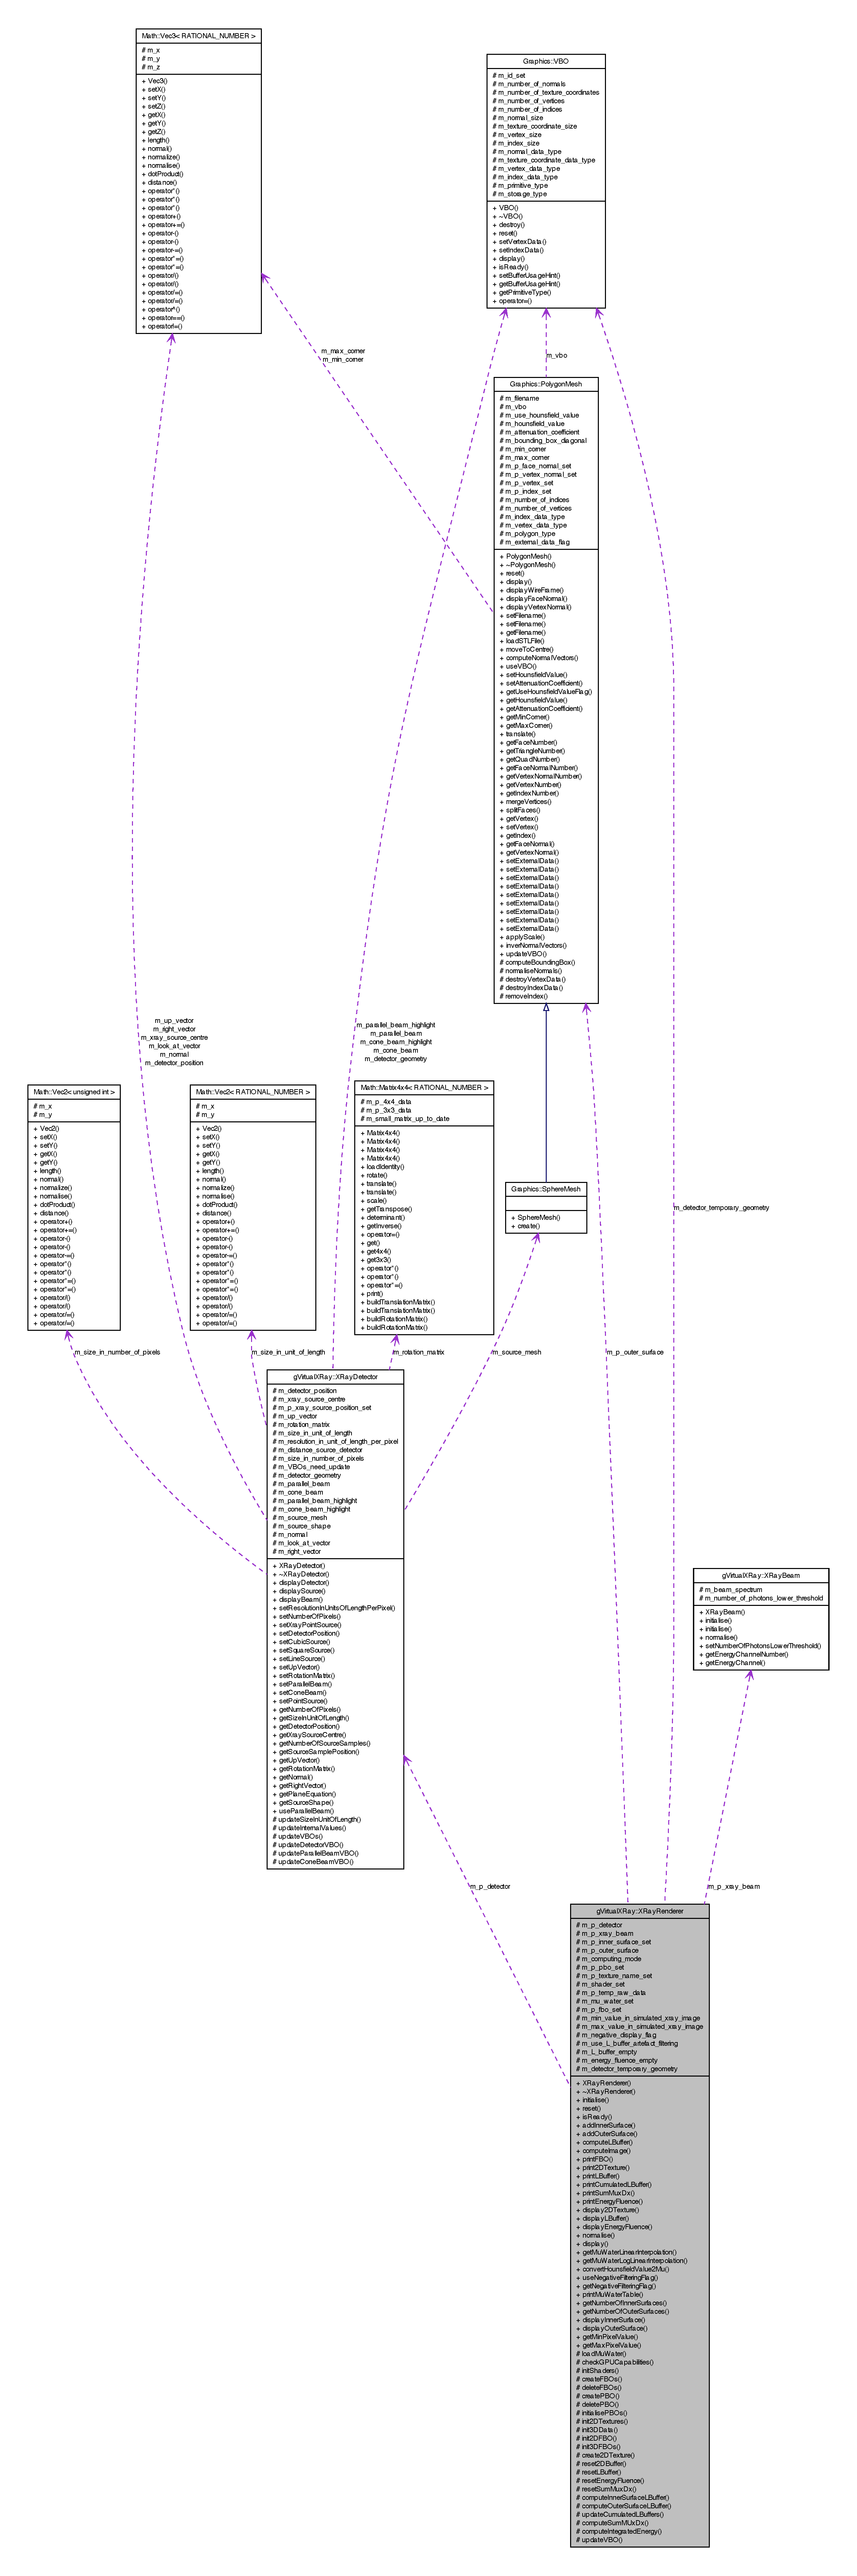
\includegraphics[height=600pt]{classg_virtual_x_ray_1_1_x_ray_renderer__coll__graph}
\end{center}
\end{figure}
\subsection*{Public Types}
\begin{DoxyCompactItemize}
\item 
enum \hyperlink{classg_virtual_x_ray_1_1_x_ray_renderer_add8cc810f7a8132fceaf3b8d32a4d558}{ComputingModeTag} \{ \hyperlink{classg_virtual_x_ray_1_1_x_ray_renderer_add8cc810f7a8132fceaf3b8d32a4d558a7348b3681da412266fd6dd21cea6d285}{OPENGL}, 
\hyperlink{classg_virtual_x_ray_1_1_x_ray_renderer_add8cc810f7a8132fceaf3b8d32a4d558a4e110903ce0c33feb2921b6729c8ea2f}{CUDA}, 
\hyperlink{classg_virtual_x_ray_1_1_x_ray_renderer_add8cc810f7a8132fceaf3b8d32a4d558a14ce0ad1224e557c26f2faf8ef9a2529}{OPENCL}
 \}
\begin{DoxyCompactList}\small\item\em Type to store the computation engine (OpenGL, CUDA, OpenCL, etc.). \end{DoxyCompactList}\item 
typedef enum \hyperlink{classg_virtual_x_ray_1_1_x_ray_renderer_add8cc810f7a8132fceaf3b8d32a4d558}{gVirtualXRay::XRayRenderer::ComputingModeTag} \hyperlink{classg_virtual_x_ray_1_1_x_ray_renderer_af306d3bab294f730af5a692f716c9f81}{ComputingMode}
\begin{DoxyCompactList}\small\item\em Type to store the computation engine (OpenGL, CUDA, OpenCL, etc.). \end{DoxyCompactList}\end{DoxyCompactItemize}
\subsection*{Public Member Functions}
\begin{DoxyCompactItemize}
\item 
\hyperlink{classg_virtual_x_ray_1_1_x_ray_renderer_af946192494b2ccfbfa2cf0e5c4c04b30}{XRayRenderer} ()
\begin{DoxyCompactList}\small\item\em Default constructor. \end{DoxyCompactList}\item 
\hyperlink{classg_virtual_x_ray_1_1_x_ray_renderer_a713b38707c30dfcb0a60f7b0e9d22ba0}{$\sim$XRayRenderer} ()
\begin{DoxyCompactList}\small\item\em Destructor. \end{DoxyCompactList}\item 
void \hyperlink{classg_virtual_x_ray_1_1_x_ray_renderer_ad9bacedb45b8f2c89eb9ed25ca82e9fa}{initialise} (\hyperlink{classg_virtual_x_ray_1_1_x_ray_renderer_af306d3bab294f730af5a692f716c9f81}{ComputingMode} aComputingMode, int anInternalTextureFormat, const \hyperlink{classg_virtual_x_ray_1_1_x_ray_detector}{XRayDetector} $\ast$apDetector, const \hyperlink{classg_virtual_x_ray_1_1_x_ray_beam}{XRayBeam} $\ast$apBeamSpectrum)
\begin{DoxyCompactList}\small\item\em Initialise the renderer. \end{DoxyCompactList}\item 
void \hyperlink{classg_virtual_x_ray_1_1_x_ray_renderer_a4653f81b7f5fd198d82d9037caf132e5}{reset} ()
\item 
bool \hyperlink{classg_virtual_x_ray_1_1_x_ray_renderer_a5b8756ac0174d619b2c7daff536b846f}{isReady} () const 
\begin{DoxyCompactList}\small\item\em Check if the renderer is ready to simulate X-\/ray images. \end{DoxyCompactList}\item 
void \hyperlink{classg_virtual_x_ray_1_1_x_ray_renderer_a65a11e213cc087fbbf83b232901ca443}{addInnerSurface} (const \hyperlink{class_graphics_1_1_polygon_mesh}{PolygonMesh} $\ast$apSurface)
\begin{DoxyCompactList}\small\item\em Add a 3D object to be rendered. It will be used as an internal surface. \end{DoxyCompactList}\item 
void \hyperlink{classg_virtual_x_ray_1_1_x_ray_renderer_aa92db653d03526432b6531f27cd54034}{addOuterSurface} (const \hyperlink{class_graphics_1_1_polygon_mesh}{PolygonMesh} $\ast$apSurface)
\begin{DoxyCompactList}\small\item\em Add a 3D object to be rendered. It will be used as an external surface. \end{DoxyCompactList}\item 
void \hyperlink{classg_virtual_x_ray_1_1_x_ray_renderer_ab0dac046f1b64af44862b6cee9e46484}{computeLBuffer} (\hyperlink{class_graphics_1_1_polygon_mesh}{PolygonMesh} \&anObject, const \hyperlink{class_math_1_1_vec3}{VEC3} \&aXRaySourceDetectorTranslation, const \hyperlink{class_math_1_1_matrix4x4}{MATRIX4} \&aModellingTransformationMatrix)
\begin{DoxyCompactList}\small\item\em Compute the L-\/buffer of a 3D object. \end{DoxyCompactList}\item 
void \hyperlink{classg_virtual_x_ray_1_1_x_ray_renderer_a99cdb12e0b645163abfa53bafc2f74a2}{computeImage} (const \hyperlink{class_math_1_1_matrix4x4}{MATRIX4} \&aModellingTransformationMatrix=\hyperlink{class_math_1_1_matrix4x4}{MATRIX4}())
\begin{DoxyCompactList}\small\item\em Compute the X-\/ray image. \end{DoxyCompactList}\item 
void \hyperlink{classg_virtual_x_ray_1_1_x_ray_renderer_a7a8fbfaab41c0cbc382c53c91a2c2a31}{printFBO} (unsigned int aFBOID, const char $\ast$aFileName)
\begin{DoxyCompactList}\small\item\em Save a FBO into a file. \end{DoxyCompactList}\item 
void \hyperlink{classg_virtual_x_ray_1_1_x_ray_renderer_a7dd8b89283ff68084488b4a8b9022c89}{print2DTexture} (unsigned int aTextureID, const char $\ast$aFileName)
\begin{DoxyCompactList}\small\item\em Save a texture into a file. \end{DoxyCompactList}\item 
void \hyperlink{classg_virtual_x_ray_1_1_x_ray_renderer_a7d3ba3f88b17419c51b7b3c7c34dc19c}{printLBuffer} (const char $\ast$aFileName)
\begin{DoxyCompactList}\small\item\em Save the current L-\/buffer into a file. \end{DoxyCompactList}\item 
void \hyperlink{classg_virtual_x_ray_1_1_x_ray_renderer_abdf17ddb1dfb9f96c6577d8aa7a6c6d8}{printCumulatedLBuffer} (const char $\ast$aFileName)
\begin{DoxyCompactList}\small\item\em Save the current cumulated L-\/buffer into a file. \end{DoxyCompactList}\item 
void \hyperlink{classg_virtual_x_ray_1_1_x_ray_renderer_a3e110bcab5cfa58ac074ba54a3549dcc}{printSumMuxDx} (const char $\ast$aFileName)
\begin{DoxyCompactList}\small\item\em Save the current Mux Dx into a file. \end{DoxyCompactList}\item 
void \hyperlink{classg_virtual_x_ray_1_1_x_ray_renderer_a5ed67ac0091620328f9e0ca11b3725d5}{printEnergyFluence} (const char $\ast$aFileName)
\begin{DoxyCompactList}\small\item\em Save the current energy fluence into a file. \end{DoxyCompactList}\item 
void \hyperlink{classg_virtual_x_ray_1_1_x_ray_renderer_a204c83d6cce239e173f2fa3679ac8820}{display2DTexture} (unsigned int aTexutreID)
\begin{DoxyCompactList}\small\item\em Display a 2D texture using OpenGL. \end{DoxyCompactList}\item 
void \hyperlink{classg_virtual_x_ray_1_1_x_ray_renderer_a34ee8ba527acf9da3199d54181521f2e}{displayLBuffer} ()
\begin{DoxyCompactList}\small\item\em Display the L-\/buffer using OpenGL. \end{DoxyCompactList}\item 
void \hyperlink{classg_virtual_x_ray_1_1_x_ray_renderer_adece8b06fc47cad618596a378361c273}{displayEnergyFluence} ()
\begin{DoxyCompactList}\small\item\em Display the energy fluence using OpenGL. \end{DoxyCompactList}\item 
void \hyperlink{classg_virtual_x_ray_1_1_x_ray_renderer_abbd6c87260c167ca3b58874114cb89ac}{normalise} ()
\begin{DoxyCompactList}\small\item\em Normalise the final result to display in OpenGL. \end{DoxyCompactList}\item 
void \hyperlink{classg_virtual_x_ray_1_1_x_ray_renderer_a3e9ed824d8c1b773fc3222abdf70c948}{display} ()
\begin{DoxyCompactList}\small\item\em Display the X-\/ray image using OpenGL. \end{DoxyCompactList}\item 
\hyperlink{namespace_utilities_a40969b96bd8d847b962e297cb79f08ce}{RATIONAL\_\-NUMBER} \hyperlink{classg_virtual_x_ray_1_1_x_ray_renderer_a834e6523f215a725d20cfc6b093e93a9}{getMuWaterLinearInterpolation} (const \hyperlink{namespace_utilities_a40969b96bd8d847b962e297cb79f08ce}{RATIONAL\_\-NUMBER} \&anIncidentEnergy)
\item 
\hyperlink{namespace_utilities_a40969b96bd8d847b962e297cb79f08ce}{RATIONAL\_\-NUMBER} \hyperlink{classg_virtual_x_ray_1_1_x_ray_renderer_ae2a99079450fe70d5c0070445296200e}{getMuWaterLogLinearInterpolation} (const \hyperlink{namespace_utilities_a40969b96bd8d847b962e297cb79f08ce}{RATIONAL\_\-NUMBER} \&anIncidentEnergy)
\item 
\hyperlink{namespace_utilities_a40969b96bd8d847b962e297cb79f08ce}{RATIONAL\_\-NUMBER} \hyperlink{classg_virtual_x_ray_1_1_x_ray_renderer_a14b80bab07a5b51b2069da606677f7ed}{convertHounsfieldValue2Mu} (const \hyperlink{namespace_utilities_a40969b96bd8d847b962e297cb79f08ce}{RATIONAL\_\-NUMBER} \&HU, const \hyperlink{namespace_utilities_a40969b96bd8d847b962e297cb79f08ce}{RATIONAL\_\-NUMBER} \&mu\_\-water) const 
\begin{DoxyCompactList}\small\item\em Convert a Hounsfield value into an attenuation coefficient. \end{DoxyCompactList}\item 
void \hyperlink{classg_virtual_x_ray_1_1_x_ray_renderer_ac2969e479dce456def60e7b88e2184a9}{useNegativeFilteringFlag} (bool aFlag=true)
\begin{DoxyCompactList}\small\item\em Display the final image in negative or not. \end{DoxyCompactList}\item 
bool \hyperlink{classg_virtual_x_ray_1_1_x_ray_renderer_a945c565e34cf7b754adbad3ed4d96191}{getNegativeFilteringFlag} () const 
\begin{DoxyCompactList}\small\item\em Accessor on the flag control the display of the final in negative. \end{DoxyCompactList}\item 
void \hyperlink{classg_virtual_x_ray_1_1_x_ray_renderer_a850046acb9a509e18766fd14ee07e035}{printMuWaterTable} (std::ostream \&anOutputStream)
\begin{DoxyCompactList}\small\item\em Output the talbe of attenuation coefficients of water into a data stream. \end{DoxyCompactList}\item 
unsigned int \hyperlink{classg_virtual_x_ray_1_1_x_ray_renderer_a490556bca3d3b345081dd6c4b51a73c0}{getNumberOfInnerSurfaces} () const 
\begin{DoxyCompactList}\small\item\em Accessor on the number of inner surfaces (e.g. an internal organ in case of a medical application). \end{DoxyCompactList}\item 
unsigned int \hyperlink{classg_virtual_x_ray_1_1_x_ray_renderer_a4db9e64934d2753e9b7eff591dc88124}{getNumberOfOuterSurfaces} () const 
\item 
void \hyperlink{classg_virtual_x_ray_1_1_x_ray_renderer_a8c6675449f169cdd75f224b03d9510d0}{displayInnerSurface} (unsigned int anIndex) const 
\begin{DoxyCompactList}\small\item\em Display a given inner surface (e.g. an internal organ in case of a medical application). \end{DoxyCompactList}\item 
void \hyperlink{classg_virtual_x_ray_1_1_x_ray_renderer_a5318d429f1d2d8fda215227228c418bb}{displayOuterSurface} () const 
\begin{DoxyCompactList}\small\item\em Display the outer surface (e.g. the skin surface in case of a medical application). \end{DoxyCompactList}\item 
\hyperlink{namespace_utilities_a40969b96bd8d847b962e297cb79f08ce}{RATIONAL\_\-NUMBER} \hyperlink{classg_virtual_x_ray_1_1_x_ray_renderer_a303d0c055e4b5841aaf9c96c6822b5e4}{getMinPixelValue} () const 
\begin{DoxyCompactList}\small\item\em Accessor on the smallest pixel intensity in the latest simulated X-\/ray image. \end{DoxyCompactList}\item 
\hyperlink{namespace_utilities_a40969b96bd8d847b962e297cb79f08ce}{RATIONAL\_\-NUMBER} \hyperlink{classg_virtual_x_ray_1_1_x_ray_renderer_aaf76470c76161d0fa6afdd4fd0324d69}{getMaxPixelValue} () const 
\begin{DoxyCompactList}\small\item\em Accessor on the greatest pixel intensity in the latest simulated X-\/ray image. \end{DoxyCompactList}\end{DoxyCompactItemize}
\subsection*{Protected Types}
\begin{DoxyCompactItemize}
\item 
typedef \hyperlink{namespace_utilities_a40969b96bd8d847b962e297cb79f08ce}{RATIONAL\_\-NUMBER} \hyperlink{classg_virtual_x_ray_1_1_x_ray_renderer_a1337efbad4ecdc7ea0054b187590596d}{PixelType}
\begin{DoxyCompactList}\small\item\em Pixel type. \end{DoxyCompactList}\end{DoxyCompactItemize}
\subsection*{Protected Member Functions}
\begin{DoxyCompactItemize}
\item 
void \hyperlink{classg_virtual_x_ray_1_1_x_ray_renderer_a1a5573eb584f679e9c1128ce500e943e}{loadMuWater} ()
\begin{DoxyCompactList}\small\item\em Load the table of water attenuation coefficients. \end{DoxyCompactList}\item 
void \hyperlink{classg_virtual_x_ray_1_1_x_ray_renderer_a5bbcfdeb612308a24c2c357fe64b1503}{checkGPUCapabilities} ()
\item 
void \hyperlink{classg_virtual_x_ray_1_1_x_ray_renderer_ae991fabec12a82228e5f678ef4c85305}{initShaders} ()
\begin{DoxyCompactList}\small\item\em Initialise the shaders. \end{DoxyCompactList}\item 
void \hyperlink{classg_virtual_x_ray_1_1_x_ray_renderer_a08f781173c61d93a46a5b3f1b76cf87b}{createFBOs} ()
\begin{DoxyCompactList}\small\item\em Create the FBOs. \end{DoxyCompactList}\item 
void \hyperlink{classg_virtual_x_ray_1_1_x_ray_renderer_a16ab1d2c97a7ac98a9f8a9e5c161d18b}{deleteFBOs} ()
\begin{DoxyCompactList}\small\item\em Delete the FBOs. \end{DoxyCompactList}\item 
void \hyperlink{classg_virtual_x_ray_1_1_x_ray_renderer_a3e578c0b4e93b04a5cb495b23ca4ec29}{createPBO} (unsigned int \&aPBO)
\begin{DoxyCompactList}\small\item\em Create a PBO. \end{DoxyCompactList}\item 
void \hyperlink{classg_virtual_x_ray_1_1_x_ray_renderer_ace71e81ac4d981e1c3474e5afabbb2d2}{deletePBO} (unsigned int \&aPBO)
\begin{DoxyCompactList}\small\item\em Delete a PBO. \end{DoxyCompactList}\item 
void \hyperlink{classg_virtual_x_ray_1_1_x_ray_renderer_ab3dbe6cad45ae0cfedbc49050433bc23}{initialisePBOs} ()
\begin{DoxyCompactList}\small\item\em Initialise the PBOs. \end{DoxyCompactList}\item 
void \hyperlink{classg_virtual_x_ray_1_1_x_ray_renderer_a7426f1da160716ac5a07ce77bef11d88}{init2DTextures} (int anInternalTextureFormat)
\begin{DoxyCompactList}\small\item\em Initialise the 2D textures. \end{DoxyCompactList}\item 
void \hyperlink{classg_virtual_x_ray_1_1_x_ray_renderer_ae19e22db29248abc1697891358ddf4ef}{init3DData} (int anInternalTextureFormat)
\begin{DoxyCompactList}\small\item\em Initialise the 3D textures. \end{DoxyCompactList}\item 
void \hyperlink{classg_virtual_x_ray_1_1_x_ray_renderer_ad0c1f3e117c0a473f7a27b760be8406b}{init2DFBO} (unsigned int aFBOIndex, unsigned int aTextureIndex)
\begin{DoxyCompactList}\small\item\em Initialise a FBO (e.g. attach textures, etc.). \end{DoxyCompactList}\item 
void \hyperlink{classg_virtual_x_ray_1_1_x_ray_renderer_a1e858d82bd7df2f02f98ce1fa700b352}{init3DFBOs} ()
\begin{DoxyCompactList}\small\item\em Initialise a FBO with a 3D texture. \end{DoxyCompactList}\item 
void \hyperlink{classg_virtual_x_ray_1_1_x_ray_renderer_ae3a251145da088ff95dd299eb5394405}{create2DTexture} (unsigned int $\ast$apTextureID, int anInternalTextureFormat)
\begin{DoxyCompactList}\small\item\em Create a 2D texture. \end{DoxyCompactList}\item 
void \hyperlink{classg_virtual_x_ray_1_1_x_ray_renderer_a9aceef4f519760a2694b0b19fe634996}{reset2DBuffer} (unsigned int aFrameBuffer)
\begin{DoxyCompactList}\small\item\em Reset the value of a FBO to 0. \end{DoxyCompactList}\item 
void \hyperlink{classg_virtual_x_ray_1_1_x_ray_renderer_a6c875c895dc36457d367b7553a2c8e9c}{resetLBuffer} ()
\begin{DoxyCompactList}\small\item\em Reset the L-\/buffer FBO to 0. \end{DoxyCompactList}\item 
void \hyperlink{classg_virtual_x_ray_1_1_x_ray_renderer_aed59e8c837471d013e5b5ea006881465}{resetEnergyFluence} ()
\begin{DoxyCompactList}\small\item\em Reset the energy fluence FBO to 0. \end{DoxyCompactList}\item 
void \hyperlink{classg_virtual_x_ray_1_1_x_ray_renderer_a9687410867e38b6d5140678b0a16c146}{resetSumMuxDx} ()
\begin{DoxyCompactList}\small\item\em Reset the Mu\_\-x $\ast$ D\_\-x FBO to 0. \end{DoxyCompactList}\item 
void \hyperlink{classg_virtual_x_ray_1_1_x_ray_renderer_aa9d6223020b229b98ba7a57eb15ec306}{computeInnerSurfaceLBuffer} (\hyperlink{class_graphics_1_1_polygon_mesh}{PolygonMesh} \&anObject, const \hyperlink{class_math_1_1_vec3}{VEC3} \&aXRaySourceSampleOffset, const \hyperlink{class_math_1_1_matrix4x4}{MATRIX4} \&aModellingTransformationMatrix)
\begin{DoxyCompactList}\small\item\em Compute the L-\/buffer of an internal object. \end{DoxyCompactList}\item 
void \hyperlink{classg_virtual_x_ray_1_1_x_ray_renderer_acb29e82c18bd5e87359301e4557aefb8}{computeOuterSurfaceLBuffer} (\hyperlink{class_graphics_1_1_polygon_mesh}{PolygonMesh} \&anObject, const \hyperlink{class_math_1_1_vec3}{VEC3} \&aXRaySourceSampleOffset, const \hyperlink{class_math_1_1_matrix4x4}{MATRIX4} \&aModellingTransformationMatrix)
\begin{DoxyCompactList}\small\item\em Compute the L-\/buffer of an external object. \end{DoxyCompactList}\item 
void \hyperlink{classg_virtual_x_ray_1_1_x_ray_renderer_a30af82b3a10279690ab2b395e6c812a6}{updateCumulatedLBuffers} (unsigned int anObjectID)
\item 
void \hyperlink{classg_virtual_x_ray_1_1_x_ray_renderer_a3190cdb7948bd2e446e44da82c39d7b1}{computeSumMUxDx} (\hyperlink{namespace_utilities_a40969b96bd8d847b962e297cb79f08ce}{RATIONAL\_\-NUMBER} HU, unsigned int anObjectID)
\begin{DoxyCompactList}\small\item\em Compute t. \end{DoxyCompactList}\item 
void \hyperlink{classg_virtual_x_ray_1_1_x_ray_renderer_a117022f350fe6b0ab342edd804f44fb8}{computeIntegratedEnergy} ()
\begin{DoxyCompactList}\small\item\em Compute the energy fluence. \end{DoxyCompactList}\item 
void \hyperlink{classg_virtual_x_ray_1_1_x_ray_renderer_ae800750bd503f2e18251c266d8e528e3}{updateVBO} ()
\begin{DoxyCompactList}\small\item\em Update the VBO of the geometry. \end{DoxyCompactList}\end{DoxyCompactItemize}
\subsection*{Protected Attributes}
\begin{DoxyCompactItemize}
\item 
\hyperlink{classg_virtual_x_ray_1_1_x_ray_detector}{XRayDetector} $\ast$ \hyperlink{classg_virtual_x_ray_1_1_x_ray_renderer_abe635fe1136fa3936fd5439cf888aad9}{m\_\-p\_\-detector}
\begin{DoxyCompactList}\small\item\em The X-\/ray detector. \end{DoxyCompactList}\item 
\hyperlink{classg_virtual_x_ray_1_1_x_ray_beam}{XRayBeam} $\ast$ \hyperlink{classg_virtual_x_ray_1_1_x_ray_renderer_a10326c78ad5b1ff35d529efa4212aa78}{m\_\-p\_\-xray\_\-beam}
\begin{DoxyCompactList}\small\item\em The X-\/ray beam. \end{DoxyCompactList}\item 
std::vector$<$ \hyperlink{class_graphics_1_1_polygon_mesh}{PolygonMesh} $\ast$ $>$ \hyperlink{classg_virtual_x_ray_1_1_x_ray_renderer_a18d3b60ab79b39221526a490935e955f}{m\_\-p\_\-inner\_\-surface\_\-set}
\begin{DoxyCompactList}\small\item\em Set of 3D geometries. \end{DoxyCompactList}\item 
\hyperlink{class_graphics_1_1_polygon_mesh}{PolygonMesh} $\ast$ \hyperlink{classg_virtual_x_ray_1_1_x_ray_renderer_a4d31028c769154394e7815f39c164bc7}{m\_\-p\_\-outer\_\-surface}
\begin{DoxyCompactList}\small\item\em The 3D geometry that will wrap the ones in m\_\-p\_\-inner\_\-surface\_\-set. \end{DoxyCompactList}\item 
\hyperlink{classg_virtual_x_ray_1_1_x_ray_renderer_af306d3bab294f730af5a692f716c9f81}{ComputingMode} \hyperlink{classg_virtual_x_ray_1_1_x_ray_renderer_acd744ca8277894c4e33c580c64e809b0}{m\_\-computing\_\-mode}
\begin{DoxyCompactList}\small\item\em The computing mode (OPENGL, CUDA, or OPENCL) \end{DoxyCompactList}\item 
std::vector$<$ unsigned int $>$ \hyperlink{classg_virtual_x_ray_1_1_x_ray_renderer_a3c98784b4ffd06d7dac0c43e20713b14}{m\_\-p\_\-pbo\_\-set}
\begin{DoxyCompactList}\small\item\em Set of PBOs. \end{DoxyCompactList}\item 
std::vector$<$ unsigned int $>$ \hyperlink{classg_virtual_x_ray_1_1_x_ray_renderer_a1075d6644118669ee6948eab5ee82f85}{m\_\-p\_\-texture\_\-name\_\-set}
\begin{DoxyCompactList}\small\item\em Set of textures. \end{DoxyCompactList}\item 
std::vector$<$ \hyperlink{class_graphics_1_1_shader}{Shader} $>$ \hyperlink{classg_virtual_x_ray_1_1_x_ray_renderer_a737acc3cdfe28c3db90dfd69dce0a203}{m\_\-shader\_\-set}
\begin{DoxyCompactList}\small\item\em Set of shaders. \end{DoxyCompactList}\item 
\hyperlink{classg_virtual_x_ray_1_1_x_ray_renderer_a1337efbad4ecdc7ea0054b187590596d}{PixelType} $\ast$ \hyperlink{classg_virtual_x_ray_1_1_x_ray_renderer_ad6c887c8da3342dffaa237115e9b933d}{m\_\-p\_\-temp\_\-raw\_\-data}
\begin{DoxyCompactList}\small\item\em The raw data of the last FBO that was loaded in the main memory. \end{DoxyCompactList}\item 
std::vector$<$ \hyperlink{classg_virtual_x_ray_1_1_attenuation_coefficient}{AttenuationCoefficient} $>$ \hyperlink{classg_virtual_x_ray_1_1_x_ray_renderer_a26aff3c3fd71edffc1559635eae312f3}{m\_\-mu\_\-water\_\-set}
\begin{DoxyCompactList}\small\item\em The table of water energy fluence coefficients. \end{DoxyCompactList}\item 
std::vector$<$ \hyperlink{class_framebuffer_object}{FramebufferObject} $\ast$ $>$ \hyperlink{classg_virtual_x_ray_1_1_x_ray_renderer_ac3df573e0519dd9809dbf5e7e762f796}{m\_\-p\_\-fbo\_\-set}
\begin{DoxyCompactList}\small\item\em The set of FBOs. \end{DoxyCompactList}\item 
\hyperlink{namespace_utilities_a40969b96bd8d847b962e297cb79f08ce}{RATIONAL\_\-NUMBER} \hyperlink{classg_virtual_x_ray_1_1_x_ray_renderer_a350d7524f24139e16a4beebf16551d52}{m\_\-min\_\-value\_\-in\_\-simulated\_\-xray\_\-image}
\begin{DoxyCompactList}\small\item\em Min value in simulated X-\/ray image. \end{DoxyCompactList}\item 
\hyperlink{namespace_utilities_a40969b96bd8d847b962e297cb79f08ce}{RATIONAL\_\-NUMBER} \hyperlink{classg_virtual_x_ray_1_1_x_ray_renderer_a5e6f1a20a2356390150648719106d4bb}{m\_\-max\_\-value\_\-in\_\-simulated\_\-xray\_\-image}
\begin{DoxyCompactList}\small\item\em Max value in simulated X-\/ray image. \end{DoxyCompactList}\item 
unsigned int \hyperlink{classg_virtual_x_ray_1_1_x_ray_renderer_a8ae2b2b8eb0fe41316fcebcb7cfcd814}{m\_\-negative\_\-display\_\-flag}
\begin{DoxyCompactList}\small\item\em Flag to display the result in negative or not. \end{DoxyCompactList}\item 
bool \hyperlink{classg_virtual_x_ray_1_1_x_ray_renderer_ade779286f936cbe987f62796e2222916}{m\_\-use\_\-L\_\-buffer\_\-artefact\_\-filtering}
\begin{DoxyCompactList}\small\item\em Flag set to true to use L-\/buffer artefact filtering. \end{DoxyCompactList}\item 
bool \hyperlink{classg_virtual_x_ray_1_1_x_ray_renderer_aca5aa1801c0c56d9c2129d53a81aa2d1}{m\_\-L\_\-buffer\_\-empty}
\begin{DoxyCompactList}\small\item\em Flag use for lazy evaluation of the L-\/Buffer. \end{DoxyCompactList}\item 
bool \hyperlink{classg_virtual_x_ray_1_1_x_ray_renderer_aab1918fd34945b6afc1d1105e946001e}{m\_\-energy\_\-fluence\_\-empty}
\begin{DoxyCompactList}\small\item\em Flag use for lazy evaluation and blending of the energy fluence. \end{DoxyCompactList}\item 
\hyperlink{class_graphics_1_1_v_b_o}{VBO} \hyperlink{classg_virtual_x_ray_1_1_x_ray_renderer_ad17a5ac822d9095a14d361a41dd2827c}{m\_\-detector\_\-temporary\_\-geometry}
\begin{DoxyCompactList}\small\item\em The VBO used to display a rectangle corresponding to the detector. \end{DoxyCompactList}\end{DoxyCompactItemize}


\subsection{Detailed Description}
\hyperlink{classg_virtual_x_ray_1_1_x_ray_renderer}{XRayRenderer} is a class to compute and renderer X-\/ray images on GPU. 

Definition at line 93 of file XRayRenderer.h.



\subsection{Member Typedef Documentation}
\hypertarget{classg_virtual_x_ray_1_1_x_ray_renderer_af306d3bab294f730af5a692f716c9f81}{
\index{gVirtualXRay::XRayRenderer@{gVirtualXRay::XRayRenderer}!ComputingMode@{ComputingMode}}
\index{ComputingMode@{ComputingMode}!gVirtualXRay::XRayRenderer@{gVirtualXRay::XRayRenderer}}
\subsubsection[{ComputingMode}]{\setlength{\rightskip}{0pt plus 5cm}typedef enum {\bf gVirtualXRay::XRayRenderer::ComputingModeTag}  {\bf gVirtualXRay::XRayRenderer::ComputingMode}}}
\label{classg_virtual_x_ray_1_1_x_ray_renderer_af306d3bab294f730af5a692f716c9f81}


Type to store the computation engine (OpenGL, CUDA, OpenCL, etc.). 

\hypertarget{classg_virtual_x_ray_1_1_x_ray_renderer_a1337efbad4ecdc7ea0054b187590596d}{
\index{gVirtualXRay::XRayRenderer@{gVirtualXRay::XRayRenderer}!PixelType@{PixelType}}
\index{PixelType@{PixelType}!gVirtualXRay::XRayRenderer@{gVirtualXRay::XRayRenderer}}
\subsubsection[{PixelType}]{\setlength{\rightskip}{0pt plus 5cm}typedef {\bf RATIONAL\_\-NUMBER} {\bf gVirtualXRay::XRayRenderer::PixelType}\hspace{0.3cm}{\ttfamily  \mbox{[}protected\mbox{]}}}}
\label{classg_virtual_x_ray_1_1_x_ray_renderer_a1337efbad4ecdc7ea0054b187590596d}


Pixel type. 



Definition at line 98 of file XRayRenderer.h.



\subsection{Member Enumeration Documentation}
\hypertarget{classg_virtual_x_ray_1_1_x_ray_renderer_add8cc810f7a8132fceaf3b8d32a4d558}{
\index{gVirtualXRay::XRayRenderer@{gVirtualXRay::XRayRenderer}!ComputingModeTag@{ComputingModeTag}}
\index{ComputingModeTag@{ComputingModeTag}!gVirtualXRay::XRayRenderer@{gVirtualXRay::XRayRenderer}}
\subsubsection[{ComputingModeTag}]{\setlength{\rightskip}{0pt plus 5cm}enum {\bf gVirtualXRay::XRayRenderer::ComputingModeTag}}}
\label{classg_virtual_x_ray_1_1_x_ray_renderer_add8cc810f7a8132fceaf3b8d32a4d558}


Type to store the computation engine (OpenGL, CUDA, OpenCL, etc.). 

\begin{Desc}
\item[Enumerator: ]\par
\begin{description}
\index{OPENGL@{OPENGL}!gVirtualXRay::XRayRenderer@{gVirtualXRay::XRayRenderer}}\index{gVirtualXRay::XRayRenderer@{gVirtualXRay::XRayRenderer}!OPENGL@{OPENGL}}\item[{\em 
\hypertarget{classg_virtual_x_ray_1_1_x_ray_renderer_add8cc810f7a8132fceaf3b8d32a4d558a7348b3681da412266fd6dd21cea6d285}{
OPENGL}
\label{classg_virtual_x_ray_1_1_x_ray_renderer_add8cc810f7a8132fceaf3b8d32a4d558a7348b3681da412266fd6dd21cea6d285}
}]Computation using OpenGL. \index{CUDA@{CUDA}!gVirtualXRay::XRayRenderer@{gVirtualXRay::XRayRenderer}}\index{gVirtualXRay::XRayRenderer@{gVirtualXRay::XRayRenderer}!CUDA@{CUDA}}\item[{\em 
\hypertarget{classg_virtual_x_ray_1_1_x_ray_renderer_add8cc810f7a8132fceaf3b8d32a4d558a4e110903ce0c33feb2921b6729c8ea2f}{
CUDA}
\label{classg_virtual_x_ray_1_1_x_ray_renderer_add8cc810f7a8132fceaf3b8d32a4d558a4e110903ce0c33feb2921b6729c8ea2f}
}]Computation using CUDA. \index{OPENCL@{OPENCL}!gVirtualXRay::XRayRenderer@{gVirtualXRay::XRayRenderer}}\index{gVirtualXRay::XRayRenderer@{gVirtualXRay::XRayRenderer}!OPENCL@{OPENCL}}\item[{\em 
\hypertarget{classg_virtual_x_ray_1_1_x_ray_renderer_add8cc810f7a8132fceaf3b8d32a4d558a14ce0ad1224e557c26f2faf8ef9a2529}{
OPENCL}
\label{classg_virtual_x_ray_1_1_x_ray_renderer_add8cc810f7a8132fceaf3b8d32a4d558a14ce0ad1224e557c26f2faf8ef9a2529}
}]Computation using OpenCL. \end{description}
\end{Desc}



Definition at line 109 of file XRayRenderer.h.



\subsection{Constructor \& Destructor Documentation}
\hypertarget{classg_virtual_x_ray_1_1_x_ray_renderer_af946192494b2ccfbfa2cf0e5c4c04b30}{
\index{gVirtualXRay::XRayRenderer@{gVirtualXRay::XRayRenderer}!XRayRenderer@{XRayRenderer}}
\index{XRayRenderer@{XRayRenderer}!gVirtualXRay::XRayRenderer@{gVirtualXRay::XRayRenderer}}
\subsubsection[{XRayRenderer}]{\setlength{\rightskip}{0pt plus 5cm}gVirtualXRay::XRayRenderer::XRayRenderer (
\begin{DoxyParamCaption}
{}
\end{DoxyParamCaption}
)}}
\label{classg_virtual_x_ray_1_1_x_ray_renderer_af946192494b2ccfbfa2cf0e5c4c04b30}


Default constructor. 

\hypertarget{classg_virtual_x_ray_1_1_x_ray_renderer_a713b38707c30dfcb0a60f7b0e9d22ba0}{
\index{gVirtualXRay::XRayRenderer@{gVirtualXRay::XRayRenderer}!$\sim$XRayRenderer@{$\sim$XRayRenderer}}
\index{$\sim$XRayRenderer@{$\sim$XRayRenderer}!gVirtualXRay::XRayRenderer@{gVirtualXRay::XRayRenderer}}
\subsubsection[{$\sim$XRayRenderer}]{\setlength{\rightskip}{0pt plus 5cm}gVirtualXRay::XRayRenderer::$\sim$XRayRenderer (
\begin{DoxyParamCaption}
{}
\end{DoxyParamCaption}
)}}
\label{classg_virtual_x_ray_1_1_x_ray_renderer_a713b38707c30dfcb0a60f7b0e9d22ba0}


Destructor. 



\subsection{Member Function Documentation}
\hypertarget{classg_virtual_x_ray_1_1_x_ray_renderer_a65a11e213cc087fbbf83b232901ca443}{
\index{gVirtualXRay::XRayRenderer@{gVirtualXRay::XRayRenderer}!addInnerSurface@{addInnerSurface}}
\index{addInnerSurface@{addInnerSurface}!gVirtualXRay::XRayRenderer@{gVirtualXRay::XRayRenderer}}
\subsubsection[{addInnerSurface}]{\setlength{\rightskip}{0pt plus 5cm}void gVirtualXRay::XRayRenderer::addInnerSurface (
\begin{DoxyParamCaption}
\item[{const {\bf PolygonMesh} $\ast$}]{apSurface}
\end{DoxyParamCaption}
)\hspace{0.3cm}{\ttfamily  \mbox{[}inline\mbox{]}}}}
\label{classg_virtual_x_ray_1_1_x_ray_renderer_a65a11e213cc087fbbf83b232901ca443}


Add a 3D object to be rendered. It will be used as an internal surface. 


\begin{DoxyParams}{Parameters}
{\em apSurface,:} & the 3D object \\
\hline
\end{DoxyParams}


Definition at line 62 of file XRayRenderer.inl.

\hypertarget{classg_virtual_x_ray_1_1_x_ray_renderer_aa92db653d03526432b6531f27cd54034}{
\index{gVirtualXRay::XRayRenderer@{gVirtualXRay::XRayRenderer}!addOuterSurface@{addOuterSurface}}
\index{addOuterSurface@{addOuterSurface}!gVirtualXRay::XRayRenderer@{gVirtualXRay::XRayRenderer}}
\subsubsection[{addOuterSurface}]{\setlength{\rightskip}{0pt plus 5cm}void gVirtualXRay::XRayRenderer::addOuterSurface (
\begin{DoxyParamCaption}
\item[{const {\bf PolygonMesh} $\ast$}]{apSurface}
\end{DoxyParamCaption}
)\hspace{0.3cm}{\ttfamily  \mbox{[}inline\mbox{]}}}}
\label{classg_virtual_x_ray_1_1_x_ray_renderer_aa92db653d03526432b6531f27cd54034}


Add a 3D object to be rendered. It will be used as an external surface. 


\begin{DoxyParams}{Parameters}
{\em apSurface,:} & the 3D object \\
\hline
\end{DoxyParams}


Definition at line 70 of file XRayRenderer.inl.

\hypertarget{classg_virtual_x_ray_1_1_x_ray_renderer_a5bbcfdeb612308a24c2c357fe64b1503}{
\index{gVirtualXRay::XRayRenderer@{gVirtualXRay::XRayRenderer}!checkGPUCapabilities@{checkGPUCapabilities}}
\index{checkGPUCapabilities@{checkGPUCapabilities}!gVirtualXRay::XRayRenderer@{gVirtualXRay::XRayRenderer}}
\subsubsection[{checkGPUCapabilities}]{\setlength{\rightskip}{0pt plus 5cm}void gVirtualXRay::XRayRenderer::checkGPUCapabilities (
\begin{DoxyParamCaption}
{}
\end{DoxyParamCaption}
)\hspace{0.3cm}{\ttfamily  \mbox{[}protected\mbox{]}}}}
\label{classg_virtual_x_ray_1_1_x_ray_renderer_a5bbcfdeb612308a24c2c357fe64b1503}
Check that the device supports all the required OpenGL extensions that are needed. \hypertarget{classg_virtual_x_ray_1_1_x_ray_renderer_a99cdb12e0b645163abfa53bafc2f74a2}{
\index{gVirtualXRay::XRayRenderer@{gVirtualXRay::XRayRenderer}!computeImage@{computeImage}}
\index{computeImage@{computeImage}!gVirtualXRay::XRayRenderer@{gVirtualXRay::XRayRenderer}}
\subsubsection[{computeImage}]{\setlength{\rightskip}{0pt plus 5cm}void gVirtualXRay::XRayRenderer::computeImage (
\begin{DoxyParamCaption}
\item[{const {\bf MATRIX4} \&}]{aModellingTransformationMatrix = {\ttfamily {\bf MATRIX4}()}}
\end{DoxyParamCaption}
)}}
\label{classg_virtual_x_ray_1_1_x_ray_renderer_a99cdb12e0b645163abfa53bafc2f74a2}


Compute the X-\/ray image. 


\begin{DoxyParams}{Parameters}
{\em aModellingTransformationMatrix,:} & a modelling transformation matrix that will be used on all the 3D objects \\
\hline
\end{DoxyParams}
\hypertarget{classg_virtual_x_ray_1_1_x_ray_renderer_aa9d6223020b229b98ba7a57eb15ec306}{
\index{gVirtualXRay::XRayRenderer@{gVirtualXRay::XRayRenderer}!computeInnerSurfaceLBuffer@{computeInnerSurfaceLBuffer}}
\index{computeInnerSurfaceLBuffer@{computeInnerSurfaceLBuffer}!gVirtualXRay::XRayRenderer@{gVirtualXRay::XRayRenderer}}
\subsubsection[{computeInnerSurfaceLBuffer}]{\setlength{\rightskip}{0pt plus 5cm}void gVirtualXRay::XRayRenderer::computeInnerSurfaceLBuffer (
\begin{DoxyParamCaption}
\item[{{\bf PolygonMesh} \&}]{anObject, }
\item[{const {\bf VEC3} \&}]{aXRaySourceSampleOffset, }
\item[{const {\bf MATRIX4} \&}]{aModellingTransformationMatrix}
\end{DoxyParamCaption}
)\hspace{0.3cm}{\ttfamily  \mbox{[}protected\mbox{]}}}}
\label{classg_virtual_x_ray_1_1_x_ray_renderer_aa9d6223020b229b98ba7a57eb15ec306}


Compute the L-\/buffer of an internal object. 


\begin{DoxyParams}{Parameters}
{\em anObject,:} & the 3D object to process \\
\hline
{\em aXRaySourceSampleOffset,:} & the translation vector to use when the source is not aligned with the detector \\
\hline
{\em aModellingTransformationMatrix,:} & the transformation matrix of the 3D object \\
\hline
\end{DoxyParams}
\hypertarget{classg_virtual_x_ray_1_1_x_ray_renderer_a117022f350fe6b0ab342edd804f44fb8}{
\index{gVirtualXRay::XRayRenderer@{gVirtualXRay::XRayRenderer}!computeIntegratedEnergy@{computeIntegratedEnergy}}
\index{computeIntegratedEnergy@{computeIntegratedEnergy}!gVirtualXRay::XRayRenderer@{gVirtualXRay::XRayRenderer}}
\subsubsection[{computeIntegratedEnergy}]{\setlength{\rightskip}{0pt plus 5cm}void gVirtualXRay::XRayRenderer::computeIntegratedEnergy (
\begin{DoxyParamCaption}
{}
\end{DoxyParamCaption}
)\hspace{0.3cm}{\ttfamily  \mbox{[}protected\mbox{]}}}}
\label{classg_virtual_x_ray_1_1_x_ray_renderer_a117022f350fe6b0ab342edd804f44fb8}


Compute the energy fluence. 

\hypertarget{classg_virtual_x_ray_1_1_x_ray_renderer_ab0dac046f1b64af44862b6cee9e46484}{
\index{gVirtualXRay::XRayRenderer@{gVirtualXRay::XRayRenderer}!computeLBuffer@{computeLBuffer}}
\index{computeLBuffer@{computeLBuffer}!gVirtualXRay::XRayRenderer@{gVirtualXRay::XRayRenderer}}
\subsubsection[{computeLBuffer}]{\setlength{\rightskip}{0pt plus 5cm}void gVirtualXRay::XRayRenderer::computeLBuffer (
\begin{DoxyParamCaption}
\item[{{\bf PolygonMesh} \&}]{anObject, }
\item[{const {\bf VEC3} \&}]{aXRaySourceDetectorTranslation, }
\item[{const {\bf MATRIX4} \&}]{aModellingTransformationMatrix}
\end{DoxyParamCaption}
)}}
\label{classg_virtual_x_ray_1_1_x_ray_renderer_ab0dac046f1b64af44862b6cee9e46484}


Compute the L-\/buffer of a 3D object. 


\begin{DoxyParams}{Parameters}
{\em anObject,:} & the 3D object to process \\
\hline
{\em aXRaySourceDetectorTranslation,:} & the translation vector to use when the source is not aligned with the detector \\
\hline
{\em aModellingTransformationMatrix,:} & the transformation matrix of the 3D object \\
\hline
\end{DoxyParams}
\hypertarget{classg_virtual_x_ray_1_1_x_ray_renderer_acb29e82c18bd5e87359301e4557aefb8}{
\index{gVirtualXRay::XRayRenderer@{gVirtualXRay::XRayRenderer}!computeOuterSurfaceLBuffer@{computeOuterSurfaceLBuffer}}
\index{computeOuterSurfaceLBuffer@{computeOuterSurfaceLBuffer}!gVirtualXRay::XRayRenderer@{gVirtualXRay::XRayRenderer}}
\subsubsection[{computeOuterSurfaceLBuffer}]{\setlength{\rightskip}{0pt plus 5cm}void gVirtualXRay::XRayRenderer::computeOuterSurfaceLBuffer (
\begin{DoxyParamCaption}
\item[{{\bf PolygonMesh} \&}]{anObject, }
\item[{const {\bf VEC3} \&}]{aXRaySourceSampleOffset, }
\item[{const {\bf MATRIX4} \&}]{aModellingTransformationMatrix}
\end{DoxyParamCaption}
)\hspace{0.3cm}{\ttfamily  \mbox{[}protected\mbox{]}}}}
\label{classg_virtual_x_ray_1_1_x_ray_renderer_acb29e82c18bd5e87359301e4557aefb8}


Compute the L-\/buffer of an external object. 


\begin{DoxyParams}{Parameters}
{\em anObject,:} & the 3D object to process \\
\hline
{\em aXRaySourceSampleOffset,:} & the translation vector to use when the source is not aligned with the detector \\
\hline
{\em aModellingTransformationMatrix,:} & the transformation matrix of the 3D object \\
\hline
\end{DoxyParams}
\hypertarget{classg_virtual_x_ray_1_1_x_ray_renderer_a3190cdb7948bd2e446e44da82c39d7b1}{
\index{gVirtualXRay::XRayRenderer@{gVirtualXRay::XRayRenderer}!computeSumMUxDx@{computeSumMUxDx}}
\index{computeSumMUxDx@{computeSumMUxDx}!gVirtualXRay::XRayRenderer@{gVirtualXRay::XRayRenderer}}
\subsubsection[{computeSumMUxDx}]{\setlength{\rightskip}{0pt plus 5cm}void gVirtualXRay::XRayRenderer::computeSumMUxDx (
\begin{DoxyParamCaption}
\item[{{\bf RATIONAL\_\-NUMBER}}]{HU, }
\item[{unsigned int}]{anObjectID}
\end{DoxyParamCaption}
)\hspace{0.3cm}{\ttfamily  \mbox{[}protected\mbox{]}}}}
\label{classg_virtual_x_ray_1_1_x_ray_renderer_a3190cdb7948bd2e446e44da82c39d7b1}


Compute t. 


\begin{DoxyParams}{Parameters}
{\em HU,:} & \\
\hline
{\em anObjectID,:} & \\
\hline
\end{DoxyParams}
\hypertarget{classg_virtual_x_ray_1_1_x_ray_renderer_a14b80bab07a5b51b2069da606677f7ed}{
\index{gVirtualXRay::XRayRenderer@{gVirtualXRay::XRayRenderer}!convertHounsfieldValue2Mu@{convertHounsfieldValue2Mu}}
\index{convertHounsfieldValue2Mu@{convertHounsfieldValue2Mu}!gVirtualXRay::XRayRenderer@{gVirtualXRay::XRayRenderer}}
\subsubsection[{convertHounsfieldValue2Mu}]{\setlength{\rightskip}{0pt plus 5cm}{\bf RATIONAL\_\-NUMBER} gVirtualXRay::XRayRenderer::convertHounsfieldValue2Mu (
\begin{DoxyParamCaption}
\item[{const {\bf RATIONAL\_\-NUMBER} \&}]{HU, }
\item[{const {\bf RATIONAL\_\-NUMBER} \&}]{mu\_\-water}
\end{DoxyParamCaption}
) const\hspace{0.3cm}{\ttfamily  \mbox{[}inline\mbox{]}}}}
\label{classg_virtual_x_ray_1_1_x_ray_renderer_a14b80bab07a5b51b2069da606677f7ed}


Convert a Hounsfield value into an attenuation coefficient. 


\begin{DoxyParams}{Parameters}
{\em HU,:} & the Hounsfield value to convert \\
\hline
{\em mu\_\-water,:} & the attenuation coefficient of water at a given energy \\
\hline
\end{DoxyParams}
\begin{DoxyReturn}{Returns}
the corresponding attenuation coefficient 
\end{DoxyReturn}


Definition at line 139 of file XRayRenderer.inl.

\hypertarget{classg_virtual_x_ray_1_1_x_ray_renderer_ae3a251145da088ff95dd299eb5394405}{
\index{gVirtualXRay::XRayRenderer@{gVirtualXRay::XRayRenderer}!create2DTexture@{create2DTexture}}
\index{create2DTexture@{create2DTexture}!gVirtualXRay::XRayRenderer@{gVirtualXRay::XRayRenderer}}
\subsubsection[{create2DTexture}]{\setlength{\rightskip}{0pt plus 5cm}void gVirtualXRay::XRayRenderer::create2DTexture (
\begin{DoxyParamCaption}
\item[{unsigned int $\ast$}]{apTextureID, }
\item[{int}]{anInternalTextureFormat}
\end{DoxyParamCaption}
)\hspace{0.3cm}{\ttfamily  \mbox{[}protected\mbox{]}}}}
\label{classg_virtual_x_ray_1_1_x_ray_renderer_ae3a251145da088ff95dd299eb5394405}


Create a 2D texture. 


\begin{DoxyParams}{Parameters}
{\em apTextureID,:} & the address on the ID of the texture \\
\hline
{\em anInternalTextureFormat,:} & the internal format in which the texture will be stored in the device \\
\hline
\end{DoxyParams}
\hypertarget{classg_virtual_x_ray_1_1_x_ray_renderer_a08f781173c61d93a46a5b3f1b76cf87b}{
\index{gVirtualXRay::XRayRenderer@{gVirtualXRay::XRayRenderer}!createFBOs@{createFBOs}}
\index{createFBOs@{createFBOs}!gVirtualXRay::XRayRenderer@{gVirtualXRay::XRayRenderer}}
\subsubsection[{createFBOs}]{\setlength{\rightskip}{0pt plus 5cm}void gVirtualXRay::XRayRenderer::createFBOs (
\begin{DoxyParamCaption}
{}
\end{DoxyParamCaption}
)\hspace{0.3cm}{\ttfamily  \mbox{[}protected\mbox{]}}}}
\label{classg_virtual_x_ray_1_1_x_ray_renderer_a08f781173c61d93a46a5b3f1b76cf87b}


Create the FBOs. 

\hypertarget{classg_virtual_x_ray_1_1_x_ray_renderer_a3e578c0b4e93b04a5cb495b23ca4ec29}{
\index{gVirtualXRay::XRayRenderer@{gVirtualXRay::XRayRenderer}!createPBO@{createPBO}}
\index{createPBO@{createPBO}!gVirtualXRay::XRayRenderer@{gVirtualXRay::XRayRenderer}}
\subsubsection[{createPBO}]{\setlength{\rightskip}{0pt plus 5cm}void gVirtualXRay::XRayRenderer::createPBO (
\begin{DoxyParamCaption}
\item[{unsigned int \&}]{aPBO}
\end{DoxyParamCaption}
)\hspace{0.3cm}{\ttfamily  \mbox{[}protected\mbox{]}}}}
\label{classg_virtual_x_ray_1_1_x_ray_renderer_a3e578c0b4e93b04a5cb495b23ca4ec29}


Create a PBO. 


\begin{DoxyParams}{Parameters}
{\em aPBO,:} & ID of the PBO to create \\
\hline
\end{DoxyParams}
\hypertarget{classg_virtual_x_ray_1_1_x_ray_renderer_a16ab1d2c97a7ac98a9f8a9e5c161d18b}{
\index{gVirtualXRay::XRayRenderer@{gVirtualXRay::XRayRenderer}!deleteFBOs@{deleteFBOs}}
\index{deleteFBOs@{deleteFBOs}!gVirtualXRay::XRayRenderer@{gVirtualXRay::XRayRenderer}}
\subsubsection[{deleteFBOs}]{\setlength{\rightskip}{0pt plus 5cm}void gVirtualXRay::XRayRenderer::deleteFBOs (
\begin{DoxyParamCaption}
{}
\end{DoxyParamCaption}
)\hspace{0.3cm}{\ttfamily  \mbox{[}protected\mbox{]}}}}
\label{classg_virtual_x_ray_1_1_x_ray_renderer_a16ab1d2c97a7ac98a9f8a9e5c161d18b}


Delete the FBOs. 

\hypertarget{classg_virtual_x_ray_1_1_x_ray_renderer_ace71e81ac4d981e1c3474e5afabbb2d2}{
\index{gVirtualXRay::XRayRenderer@{gVirtualXRay::XRayRenderer}!deletePBO@{deletePBO}}
\index{deletePBO@{deletePBO}!gVirtualXRay::XRayRenderer@{gVirtualXRay::XRayRenderer}}
\subsubsection[{deletePBO}]{\setlength{\rightskip}{0pt plus 5cm}void gVirtualXRay::XRayRenderer::deletePBO (
\begin{DoxyParamCaption}
\item[{unsigned int \&}]{aPBO}
\end{DoxyParamCaption}
)\hspace{0.3cm}{\ttfamily  \mbox{[}protected\mbox{]}}}}
\label{classg_virtual_x_ray_1_1_x_ray_renderer_ace71e81ac4d981e1c3474e5afabbb2d2}


Delete a PBO. 


\begin{DoxyParams}{Parameters}
{\em aPBO,:} & ID of the PBO to delete \\
\hline
\end{DoxyParams}
\hypertarget{classg_virtual_x_ray_1_1_x_ray_renderer_a3e9ed824d8c1b773fc3222abdf70c948}{
\index{gVirtualXRay::XRayRenderer@{gVirtualXRay::XRayRenderer}!display@{display}}
\index{display@{display}!gVirtualXRay::XRayRenderer@{gVirtualXRay::XRayRenderer}}
\subsubsection[{display}]{\setlength{\rightskip}{0pt plus 5cm}void gVirtualXRay::XRayRenderer::display (
\begin{DoxyParamCaption}
{}
\end{DoxyParamCaption}
)}}
\label{classg_virtual_x_ray_1_1_x_ray_renderer_a3e9ed824d8c1b773fc3222abdf70c948}


Display the X-\/ray image using OpenGL. 

\hypertarget{classg_virtual_x_ray_1_1_x_ray_renderer_a204c83d6cce239e173f2fa3679ac8820}{
\index{gVirtualXRay::XRayRenderer@{gVirtualXRay::XRayRenderer}!display2DTexture@{display2DTexture}}
\index{display2DTexture@{display2DTexture}!gVirtualXRay::XRayRenderer@{gVirtualXRay::XRayRenderer}}
\subsubsection[{display2DTexture}]{\setlength{\rightskip}{0pt plus 5cm}void gVirtualXRay::XRayRenderer::display2DTexture (
\begin{DoxyParamCaption}
\item[{unsigned int}]{aTexutreID}
\end{DoxyParamCaption}
)}}
\label{classg_virtual_x_ray_1_1_x_ray_renderer_a204c83d6cce239e173f2fa3679ac8820}


Display a 2D texture using OpenGL. 

\hypertarget{classg_virtual_x_ray_1_1_x_ray_renderer_adece8b06fc47cad618596a378361c273}{
\index{gVirtualXRay::XRayRenderer@{gVirtualXRay::XRayRenderer}!displayEnergyFluence@{displayEnergyFluence}}
\index{displayEnergyFluence@{displayEnergyFluence}!gVirtualXRay::XRayRenderer@{gVirtualXRay::XRayRenderer}}
\subsubsection[{displayEnergyFluence}]{\setlength{\rightskip}{0pt plus 5cm}void gVirtualXRay::XRayRenderer::displayEnergyFluence (
\begin{DoxyParamCaption}
{}
\end{DoxyParamCaption}
)}}
\label{classg_virtual_x_ray_1_1_x_ray_renderer_adece8b06fc47cad618596a378361c273}


Display the energy fluence using OpenGL. 

\hypertarget{classg_virtual_x_ray_1_1_x_ray_renderer_a8c6675449f169cdd75f224b03d9510d0}{
\index{gVirtualXRay::XRayRenderer@{gVirtualXRay::XRayRenderer}!displayInnerSurface@{displayInnerSurface}}
\index{displayInnerSurface@{displayInnerSurface}!gVirtualXRay::XRayRenderer@{gVirtualXRay::XRayRenderer}}
\subsubsection[{displayInnerSurface}]{\setlength{\rightskip}{0pt plus 5cm}void gVirtualXRay::XRayRenderer::displayInnerSurface (
\begin{DoxyParamCaption}
\item[{unsigned int}]{anIndex}
\end{DoxyParamCaption}
) const\hspace{0.3cm}{\ttfamily  \mbox{[}inline\mbox{]}}}}
\label{classg_virtual_x_ray_1_1_x_ray_renderer_a8c6675449f169cdd75f224b03d9510d0}


Display a given inner surface (e.g. an internal organ in case of a medical application). 


\begin{DoxyParams}{Parameters}
{\em anIndex,:} & the index of the inner surface to display \\
\hline
\end{DoxyParams}


Definition at line 171 of file XRayRenderer.inl.

\hypertarget{classg_virtual_x_ray_1_1_x_ray_renderer_a34ee8ba527acf9da3199d54181521f2e}{
\index{gVirtualXRay::XRayRenderer@{gVirtualXRay::XRayRenderer}!displayLBuffer@{displayLBuffer}}
\index{displayLBuffer@{displayLBuffer}!gVirtualXRay::XRayRenderer@{gVirtualXRay::XRayRenderer}}
\subsubsection[{displayLBuffer}]{\setlength{\rightskip}{0pt plus 5cm}void gVirtualXRay::XRayRenderer::displayLBuffer (
\begin{DoxyParamCaption}
{}
\end{DoxyParamCaption}
)}}
\label{classg_virtual_x_ray_1_1_x_ray_renderer_a34ee8ba527acf9da3199d54181521f2e}


Display the L-\/buffer using OpenGL. 

\hypertarget{classg_virtual_x_ray_1_1_x_ray_renderer_a5318d429f1d2d8fda215227228c418bb}{
\index{gVirtualXRay::XRayRenderer@{gVirtualXRay::XRayRenderer}!displayOuterSurface@{displayOuterSurface}}
\index{displayOuterSurface@{displayOuterSurface}!gVirtualXRay::XRayRenderer@{gVirtualXRay::XRayRenderer}}
\subsubsection[{displayOuterSurface}]{\setlength{\rightskip}{0pt plus 5cm}void gVirtualXRay::XRayRenderer::displayOuterSurface (
\begin{DoxyParamCaption}
{}
\end{DoxyParamCaption}
) const\hspace{0.3cm}{\ttfamily  \mbox{[}inline\mbox{]}}}}
\label{classg_virtual_x_ray_1_1_x_ray_renderer_a5318d429f1d2d8fda215227228c418bb}


Display the outer surface (e.g. the skin surface in case of a medical application). 



Definition at line 184 of file XRayRenderer.inl.

\hypertarget{classg_virtual_x_ray_1_1_x_ray_renderer_aaf76470c76161d0fa6afdd4fd0324d69}{
\index{gVirtualXRay::XRayRenderer@{gVirtualXRay::XRayRenderer}!getMaxPixelValue@{getMaxPixelValue}}
\index{getMaxPixelValue@{getMaxPixelValue}!gVirtualXRay::XRayRenderer@{gVirtualXRay::XRayRenderer}}
\subsubsection[{getMaxPixelValue}]{\setlength{\rightskip}{0pt plus 5cm}{\bf RATIONAL\_\-NUMBER} gVirtualXRay::XRayRenderer::getMaxPixelValue (
\begin{DoxyParamCaption}
{}
\end{DoxyParamCaption}
) const\hspace{0.3cm}{\ttfamily  \mbox{[}inline\mbox{]}}}}
\label{classg_virtual_x_ray_1_1_x_ray_renderer_aaf76470c76161d0fa6afdd4fd0324d69}


Accessor on the greatest pixel intensity in the latest simulated X-\/ray image. 

\begin{DoxyReturn}{Returns}
the max value in simulated X-\/ray image 
\end{DoxyReturn}


Definition at line 205 of file XRayRenderer.inl.

\hypertarget{classg_virtual_x_ray_1_1_x_ray_renderer_a303d0c055e4b5841aaf9c96c6822b5e4}{
\index{gVirtualXRay::XRayRenderer@{gVirtualXRay::XRayRenderer}!getMinPixelValue@{getMinPixelValue}}
\index{getMinPixelValue@{getMinPixelValue}!gVirtualXRay::XRayRenderer@{gVirtualXRay::XRayRenderer}}
\subsubsection[{getMinPixelValue}]{\setlength{\rightskip}{0pt plus 5cm}{\bf RATIONAL\_\-NUMBER} gVirtualXRay::XRayRenderer::getMinPixelValue (
\begin{DoxyParamCaption}
{}
\end{DoxyParamCaption}
) const\hspace{0.3cm}{\ttfamily  \mbox{[}inline\mbox{]}}}}
\label{classg_virtual_x_ray_1_1_x_ray_renderer_a303d0c055e4b5841aaf9c96c6822b5e4}


Accessor on the smallest pixel intensity in the latest simulated X-\/ray image. 

\begin{DoxyReturn}{Returns}
the min value in simulated X-\/ray image 
\end{DoxyReturn}


Definition at line 197 of file XRayRenderer.inl.

\hypertarget{classg_virtual_x_ray_1_1_x_ray_renderer_a834e6523f215a725d20cfc6b093e93a9}{
\index{gVirtualXRay::XRayRenderer@{gVirtualXRay::XRayRenderer}!getMuWaterLinearInterpolation@{getMuWaterLinearInterpolation}}
\index{getMuWaterLinearInterpolation@{getMuWaterLinearInterpolation}!gVirtualXRay::XRayRenderer@{gVirtualXRay::XRayRenderer}}
\subsubsection[{getMuWaterLinearInterpolation}]{\setlength{\rightskip}{0pt plus 5cm}{\bf RATIONAL\_\-NUMBER} gVirtualXRay::XRayRenderer::getMuWaterLinearInterpolation (
\begin{DoxyParamCaption}
\item[{const {\bf RATIONAL\_\-NUMBER} \&}]{anIncidentEnergy}
\end{DoxyParamCaption}
)}}
\label{classg_virtual_x_ray_1_1_x_ray_renderer_a834e6523f215a725d20cfc6b093e93a9}
Get the attenuation coefficient of water for a given energy. The value is computed using linear interpolation. 
\begin{DoxyParams}{Parameters}
{\em anIncidentEnergy,:} & the energy \\
\hline
\end{DoxyParams}
\begin{DoxyReturn}{Returns}
the corresponding attenuation coefficient of water 
\end{DoxyReturn}
\hypertarget{classg_virtual_x_ray_1_1_x_ray_renderer_ae2a99079450fe70d5c0070445296200e}{
\index{gVirtualXRay::XRayRenderer@{gVirtualXRay::XRayRenderer}!getMuWaterLogLinearInterpolation@{getMuWaterLogLinearInterpolation}}
\index{getMuWaterLogLinearInterpolation@{getMuWaterLogLinearInterpolation}!gVirtualXRay::XRayRenderer@{gVirtualXRay::XRayRenderer}}
\subsubsection[{getMuWaterLogLinearInterpolation}]{\setlength{\rightskip}{0pt plus 5cm}{\bf RATIONAL\_\-NUMBER} gVirtualXRay::XRayRenderer::getMuWaterLogLinearInterpolation (
\begin{DoxyParamCaption}
\item[{const {\bf RATIONAL\_\-NUMBER} \&}]{anIncidentEnergy}
\end{DoxyParamCaption}
)}}
\label{classg_virtual_x_ray_1_1_x_ray_renderer_ae2a99079450fe70d5c0070445296200e}
Get the attenuation coefficient of water for a given energy. The value is computed using linear interpolation on a logarithmic scale. 
\begin{DoxyParams}{Parameters}
{\em anIncidentEnergy,:} & the energy \\
\hline
\end{DoxyParams}
\begin{DoxyReturn}{Returns}
the corresponding attenuation coefficient of water 
\end{DoxyReturn}
\hypertarget{classg_virtual_x_ray_1_1_x_ray_renderer_a945c565e34cf7b754adbad3ed4d96191}{
\index{gVirtualXRay::XRayRenderer@{gVirtualXRay::XRayRenderer}!getNegativeFilteringFlag@{getNegativeFilteringFlag}}
\index{getNegativeFilteringFlag@{getNegativeFilteringFlag}!gVirtualXRay::XRayRenderer@{gVirtualXRay::XRayRenderer}}
\subsubsection[{getNegativeFilteringFlag}]{\setlength{\rightskip}{0pt plus 5cm}bool gVirtualXRay::XRayRenderer::getNegativeFilteringFlag (
\begin{DoxyParamCaption}
{}
\end{DoxyParamCaption}
) const\hspace{0.3cm}{\ttfamily  \mbox{[}inline\mbox{]}}}}
\label{classg_virtual_x_ray_1_1_x_ray_renderer_a945c565e34cf7b754adbad3ed4d96191}


Accessor on the flag control the display of the final in negative. 

\begin{DoxyReturn}{Returns}
true if the final image is displayed in negative, false it is not 
\end{DoxyReturn}


Definition at line 54 of file XRayRenderer.inl.

\hypertarget{classg_virtual_x_ray_1_1_x_ray_renderer_a490556bca3d3b345081dd6c4b51a73c0}{
\index{gVirtualXRay::XRayRenderer@{gVirtualXRay::XRayRenderer}!getNumberOfInnerSurfaces@{getNumberOfInnerSurfaces}}
\index{getNumberOfInnerSurfaces@{getNumberOfInnerSurfaces}!gVirtualXRay::XRayRenderer@{gVirtualXRay::XRayRenderer}}
\subsubsection[{getNumberOfInnerSurfaces}]{\setlength{\rightskip}{0pt plus 5cm}unsigned int gVirtualXRay::XRayRenderer::getNumberOfInnerSurfaces (
\begin{DoxyParamCaption}
{}
\end{DoxyParamCaption}
) const\hspace{0.3cm}{\ttfamily  \mbox{[}inline\mbox{]}}}}
\label{classg_virtual_x_ray_1_1_x_ray_renderer_a490556bca3d3b345081dd6c4b51a73c0}


Accessor on the number of inner surfaces (e.g. an internal organ in case of a medical application). 

\begin{DoxyReturn}{Returns}
the number of inner surfaces 
\end{DoxyReturn}


Definition at line 148 of file XRayRenderer.inl.

\hypertarget{classg_virtual_x_ray_1_1_x_ray_renderer_a4db9e64934d2753e9b7eff591dc88124}{
\index{gVirtualXRay::XRayRenderer@{gVirtualXRay::XRayRenderer}!getNumberOfOuterSurfaces@{getNumberOfOuterSurfaces}}
\index{getNumberOfOuterSurfaces@{getNumberOfOuterSurfaces}!gVirtualXRay::XRayRenderer@{gVirtualXRay::XRayRenderer}}
\subsubsection[{getNumberOfOuterSurfaces}]{\setlength{\rightskip}{0pt plus 5cm}unsigned int gVirtualXRay::XRayRenderer::getNumberOfOuterSurfaces (
\begin{DoxyParamCaption}
{}
\end{DoxyParamCaption}
) const\hspace{0.3cm}{\ttfamily  \mbox{[}inline\mbox{]}}}}
\label{classg_virtual_x_ray_1_1_x_ray_renderer_a4db9e64934d2753e9b7eff591dc88124}
Accessor on the number of outer surfaces (e.g. the skin surface in case of a medical application). This value is either equal to 0 or 1. \begin{DoxyReturn}{Returns}
the number of outer surfaces 
\end{DoxyReturn}


Definition at line 156 of file XRayRenderer.inl.

\hypertarget{classg_virtual_x_ray_1_1_x_ray_renderer_ad0c1f3e117c0a473f7a27b760be8406b}{
\index{gVirtualXRay::XRayRenderer@{gVirtualXRay::XRayRenderer}!init2DFBO@{init2DFBO}}
\index{init2DFBO@{init2DFBO}!gVirtualXRay::XRayRenderer@{gVirtualXRay::XRayRenderer}}
\subsubsection[{init2DFBO}]{\setlength{\rightskip}{0pt plus 5cm}void gVirtualXRay::XRayRenderer::init2DFBO (
\begin{DoxyParamCaption}
\item[{unsigned int}]{aFBOIndex, }
\item[{unsigned int}]{aTextureIndex}
\end{DoxyParamCaption}
)\hspace{0.3cm}{\ttfamily  \mbox{[}protected\mbox{]}}}}
\label{classg_virtual_x_ray_1_1_x_ray_renderer_ad0c1f3e117c0a473f7a27b760be8406b}


Initialise a FBO (e.g. attach textures, etc.). 


\begin{DoxyParams}{Parameters}
{\em aFBOIndex,:} & the FBO to initialise \\
\hline
{\em aTextureIndex,:} & the texture to attach \\
\hline
\end{DoxyParams}
\hypertarget{classg_virtual_x_ray_1_1_x_ray_renderer_a7426f1da160716ac5a07ce77bef11d88}{
\index{gVirtualXRay::XRayRenderer@{gVirtualXRay::XRayRenderer}!init2DTextures@{init2DTextures}}
\index{init2DTextures@{init2DTextures}!gVirtualXRay::XRayRenderer@{gVirtualXRay::XRayRenderer}}
\subsubsection[{init2DTextures}]{\setlength{\rightskip}{0pt plus 5cm}void gVirtualXRay::XRayRenderer::init2DTextures (
\begin{DoxyParamCaption}
\item[{int}]{anInternalTextureFormat}
\end{DoxyParamCaption}
)\hspace{0.3cm}{\ttfamily  \mbox{[}inline, protected\mbox{]}}}}
\label{classg_virtual_x_ray_1_1_x_ray_renderer_a7426f1da160716ac5a07ce77bef11d88}


Initialise the 2D textures. 


\begin{DoxyParams}{Parameters}
{\em anInternalTextureFormat,:} & the internal format in which OpenGL textures will be stored (GL\_\-RGB16F\_\-ARB, or GL\_\-RGB32F\_\-ARB) \\
\hline
\end{DoxyParams}


Definition at line 121 of file XRayRenderer.inl.

\hypertarget{classg_virtual_x_ray_1_1_x_ray_renderer_ae19e22db29248abc1697891358ddf4ef}{
\index{gVirtualXRay::XRayRenderer@{gVirtualXRay::XRayRenderer}!init3DData@{init3DData}}
\index{init3DData@{init3DData}!gVirtualXRay::XRayRenderer@{gVirtualXRay::XRayRenderer}}
\subsubsection[{init3DData}]{\setlength{\rightskip}{0pt plus 5cm}void gVirtualXRay::XRayRenderer::init3DData (
\begin{DoxyParamCaption}
\item[{int}]{anInternalTextureFormat}
\end{DoxyParamCaption}
)\hspace{0.3cm}{\ttfamily  \mbox{[}protected\mbox{]}}}}
\label{classg_virtual_x_ray_1_1_x_ray_renderer_ae19e22db29248abc1697891358ddf4ef}


Initialise the 3D textures. 


\begin{DoxyParams}{Parameters}
{\em anInternalTextureFormat,:} & the internal format in which OpenGL textures will be stored (GL\_\-RGB16F\_\-ARB, or GL\_\-RGB32F\_\-ARB) \\
\hline
\end{DoxyParams}
\hypertarget{classg_virtual_x_ray_1_1_x_ray_renderer_a1e858d82bd7df2f02f98ce1fa700b352}{
\index{gVirtualXRay::XRayRenderer@{gVirtualXRay::XRayRenderer}!init3DFBOs@{init3DFBOs}}
\index{init3DFBOs@{init3DFBOs}!gVirtualXRay::XRayRenderer@{gVirtualXRay::XRayRenderer}}
\subsubsection[{init3DFBOs}]{\setlength{\rightskip}{0pt plus 5cm}void gVirtualXRay::XRayRenderer::init3DFBOs (
\begin{DoxyParamCaption}
{}
\end{DoxyParamCaption}
)\hspace{0.3cm}{\ttfamily  \mbox{[}protected\mbox{]}}}}
\label{classg_virtual_x_ray_1_1_x_ray_renderer_a1e858d82bd7df2f02f98ce1fa700b352}


Initialise a FBO with a 3D texture. 

\hypertarget{classg_virtual_x_ray_1_1_x_ray_renderer_ad9bacedb45b8f2c89eb9ed25ca82e9fa}{
\index{gVirtualXRay::XRayRenderer@{gVirtualXRay::XRayRenderer}!initialise@{initialise}}
\index{initialise@{initialise}!gVirtualXRay::XRayRenderer@{gVirtualXRay::XRayRenderer}}
\subsubsection[{initialise}]{\setlength{\rightskip}{0pt plus 5cm}void gVirtualXRay::XRayRenderer::initialise (
\begin{DoxyParamCaption}
\item[{{\bf ComputingMode}}]{aComputingMode, }
\item[{int}]{anInternalTextureFormat, }
\item[{const {\bf XRayDetector} $\ast$}]{apDetector, }
\item[{const {\bf XRayBeam} $\ast$}]{apBeamSpectrum}
\end{DoxyParamCaption}
)}}
\label{classg_virtual_x_ray_1_1_x_ray_renderer_ad9bacedb45b8f2c89eb9ed25ca82e9fa}


Initialise the renderer. 


\begin{DoxyParams}{Parameters}
{\em aComputingMode,:} & the computing mode (OPENGL, CUDA, or OPENCL) \\
\hline
{\em anInternalTextureFormat,:} & the internal format in which OpenGL textures will be stored (GL\_\-RGB16F\_\-ARB, or GL\_\-RGB32F\_\-ARB) \\
\hline
{\em apDetector,:} & the X-\/ray detector that will be used \\
\hline
{\em apBeamSpectrum,:} & the X-\/ray beam spectrum \\
\hline
\end{DoxyParams}
\hypertarget{classg_virtual_x_ray_1_1_x_ray_renderer_ab3dbe6cad45ae0cfedbc49050433bc23}{
\index{gVirtualXRay::XRayRenderer@{gVirtualXRay::XRayRenderer}!initialisePBOs@{initialisePBOs}}
\index{initialisePBOs@{initialisePBOs}!gVirtualXRay::XRayRenderer@{gVirtualXRay::XRayRenderer}}
\subsubsection[{initialisePBOs}]{\setlength{\rightskip}{0pt plus 5cm}void gVirtualXRay::XRayRenderer::initialisePBOs (
\begin{DoxyParamCaption}
{}
\end{DoxyParamCaption}
)\hspace{0.3cm}{\ttfamily  \mbox{[}inline, protected\mbox{]}}}}
\label{classg_virtual_x_ray_1_1_x_ray_renderer_ab3dbe6cad45ae0cfedbc49050433bc23}


Initialise the PBOs. 



Definition at line 91 of file XRayRenderer.inl.

\hypertarget{classg_virtual_x_ray_1_1_x_ray_renderer_ae991fabec12a82228e5f678ef4c85305}{
\index{gVirtualXRay::XRayRenderer@{gVirtualXRay::XRayRenderer}!initShaders@{initShaders}}
\index{initShaders@{initShaders}!gVirtualXRay::XRayRenderer@{gVirtualXRay::XRayRenderer}}
\subsubsection[{initShaders}]{\setlength{\rightskip}{0pt plus 5cm}void gVirtualXRay::XRayRenderer::initShaders (
\begin{DoxyParamCaption}
{}
\end{DoxyParamCaption}
)\hspace{0.3cm}{\ttfamily  \mbox{[}protected\mbox{]}}}}
\label{classg_virtual_x_ray_1_1_x_ray_renderer_ae991fabec12a82228e5f678ef4c85305}


Initialise the shaders. 

\hypertarget{classg_virtual_x_ray_1_1_x_ray_renderer_a5b8756ac0174d619b2c7daff536b846f}{
\index{gVirtualXRay::XRayRenderer@{gVirtualXRay::XRayRenderer}!isReady@{isReady}}
\index{isReady@{isReady}!gVirtualXRay::XRayRenderer@{gVirtualXRay::XRayRenderer}}
\subsubsection[{isReady}]{\setlength{\rightskip}{0pt plus 5cm}bool gVirtualXRay::XRayRenderer::isReady (
\begin{DoxyParamCaption}
{}
\end{DoxyParamCaption}
) const}}
\label{classg_virtual_x_ray_1_1_x_ray_renderer_a5b8756ac0174d619b2c7daff536b846f}


Check if the renderer is ready to simulate X-\/ray images. 

\begin{DoxyReturn}{Returns}
true if the renderer is ready, false if it is not 
\end{DoxyReturn}
\hypertarget{classg_virtual_x_ray_1_1_x_ray_renderer_a1a5573eb584f679e9c1128ce500e943e}{
\index{gVirtualXRay::XRayRenderer@{gVirtualXRay::XRayRenderer}!loadMuWater@{loadMuWater}}
\index{loadMuWater@{loadMuWater}!gVirtualXRay::XRayRenderer@{gVirtualXRay::XRayRenderer}}
\subsubsection[{loadMuWater}]{\setlength{\rightskip}{0pt plus 5cm}void gVirtualXRay::XRayRenderer::loadMuWater (
\begin{DoxyParamCaption}
{}
\end{DoxyParamCaption}
)\hspace{0.3cm}{\ttfamily  \mbox{[}protected\mbox{]}}}}
\label{classg_virtual_x_ray_1_1_x_ray_renderer_a1a5573eb584f679e9c1128ce500e943e}


Load the table of water attenuation coefficients. 

\hypertarget{classg_virtual_x_ray_1_1_x_ray_renderer_abbd6c87260c167ca3b58874114cb89ac}{
\index{gVirtualXRay::XRayRenderer@{gVirtualXRay::XRayRenderer}!normalise@{normalise}}
\index{normalise@{normalise}!gVirtualXRay::XRayRenderer@{gVirtualXRay::XRayRenderer}}
\subsubsection[{normalise}]{\setlength{\rightskip}{0pt plus 5cm}void gVirtualXRay::XRayRenderer::normalise (
\begin{DoxyParamCaption}
{}
\end{DoxyParamCaption}
)}}
\label{classg_virtual_x_ray_1_1_x_ray_renderer_abbd6c87260c167ca3b58874114cb89ac}


Normalise the final result to display in OpenGL. 

\hypertarget{classg_virtual_x_ray_1_1_x_ray_renderer_a7dd8b89283ff68084488b4a8b9022c89}{
\index{gVirtualXRay::XRayRenderer@{gVirtualXRay::XRayRenderer}!print2DTexture@{print2DTexture}}
\index{print2DTexture@{print2DTexture}!gVirtualXRay::XRayRenderer@{gVirtualXRay::XRayRenderer}}
\subsubsection[{print2DTexture}]{\setlength{\rightskip}{0pt plus 5cm}void gVirtualXRay::XRayRenderer::print2DTexture (
\begin{DoxyParamCaption}
\item[{unsigned int}]{aTextureID, }
\item[{const char $\ast$}]{aFileName}
\end{DoxyParamCaption}
)}}
\label{classg_virtual_x_ray_1_1_x_ray_renderer_a7dd8b89283ff68084488b4a8b9022c89}


Save a texture into a file. 


\begin{DoxyParams}{Parameters}
{\em aTextureID,:} & the ID of the texture \\
\hline
{\em aFileName,:} & the file name \\
\hline
\end{DoxyParams}
\hypertarget{classg_virtual_x_ray_1_1_x_ray_renderer_abdf17ddb1dfb9f96c6577d8aa7a6c6d8}{
\index{gVirtualXRay::XRayRenderer@{gVirtualXRay::XRayRenderer}!printCumulatedLBuffer@{printCumulatedLBuffer}}
\index{printCumulatedLBuffer@{printCumulatedLBuffer}!gVirtualXRay::XRayRenderer@{gVirtualXRay::XRayRenderer}}
\subsubsection[{printCumulatedLBuffer}]{\setlength{\rightskip}{0pt plus 5cm}void gVirtualXRay::XRayRenderer::printCumulatedLBuffer (
\begin{DoxyParamCaption}
\item[{const char $\ast$}]{aFileName}
\end{DoxyParamCaption}
)}}
\label{classg_virtual_x_ray_1_1_x_ray_renderer_abdf17ddb1dfb9f96c6577d8aa7a6c6d8}


Save the current cumulated L-\/buffer into a file. 


\begin{DoxyParams}{Parameters}
{\em aFileName,:} & the file name \\
\hline
\end{DoxyParams}
\hypertarget{classg_virtual_x_ray_1_1_x_ray_renderer_a5ed67ac0091620328f9e0ca11b3725d5}{
\index{gVirtualXRay::XRayRenderer@{gVirtualXRay::XRayRenderer}!printEnergyFluence@{printEnergyFluence}}
\index{printEnergyFluence@{printEnergyFluence}!gVirtualXRay::XRayRenderer@{gVirtualXRay::XRayRenderer}}
\subsubsection[{printEnergyFluence}]{\setlength{\rightskip}{0pt plus 5cm}void gVirtualXRay::XRayRenderer::printEnergyFluence (
\begin{DoxyParamCaption}
\item[{const char $\ast$}]{aFileName}
\end{DoxyParamCaption}
)}}
\label{classg_virtual_x_ray_1_1_x_ray_renderer_a5ed67ac0091620328f9e0ca11b3725d5}


Save the current energy fluence into a file. 


\begin{DoxyParams}{Parameters}
{\em aFileName,:} & the file name \\
\hline
\end{DoxyParams}
\hypertarget{classg_virtual_x_ray_1_1_x_ray_renderer_a7a8fbfaab41c0cbc382c53c91a2c2a31}{
\index{gVirtualXRay::XRayRenderer@{gVirtualXRay::XRayRenderer}!printFBO@{printFBO}}
\index{printFBO@{printFBO}!gVirtualXRay::XRayRenderer@{gVirtualXRay::XRayRenderer}}
\subsubsection[{printFBO}]{\setlength{\rightskip}{0pt plus 5cm}void gVirtualXRay::XRayRenderer::printFBO (
\begin{DoxyParamCaption}
\item[{unsigned int}]{aFBOID, }
\item[{const char $\ast$}]{aFileName}
\end{DoxyParamCaption}
)}}
\label{classg_virtual_x_ray_1_1_x_ray_renderer_a7a8fbfaab41c0cbc382c53c91a2c2a31}


Save a FBO into a file. 


\begin{DoxyParams}{Parameters}
{\em aFBOID,:} & the ID of the FBO \\
\hline
{\em aFileName,:} & the file name \\
\hline
\end{DoxyParams}
\hypertarget{classg_virtual_x_ray_1_1_x_ray_renderer_a7d3ba3f88b17419c51b7b3c7c34dc19c}{
\index{gVirtualXRay::XRayRenderer@{gVirtualXRay::XRayRenderer}!printLBuffer@{printLBuffer}}
\index{printLBuffer@{printLBuffer}!gVirtualXRay::XRayRenderer@{gVirtualXRay::XRayRenderer}}
\subsubsection[{printLBuffer}]{\setlength{\rightskip}{0pt plus 5cm}void gVirtualXRay::XRayRenderer::printLBuffer (
\begin{DoxyParamCaption}
\item[{const char $\ast$}]{aFileName}
\end{DoxyParamCaption}
)}}
\label{classg_virtual_x_ray_1_1_x_ray_renderer_a7d3ba3f88b17419c51b7b3c7c34dc19c}


Save the current L-\/buffer into a file. 


\begin{DoxyParams}{Parameters}
{\em aFileName,:} & the file name \\
\hline
\end{DoxyParams}
\hypertarget{classg_virtual_x_ray_1_1_x_ray_renderer_a850046acb9a509e18766fd14ee07e035}{
\index{gVirtualXRay::XRayRenderer@{gVirtualXRay::XRayRenderer}!printMuWaterTable@{printMuWaterTable}}
\index{printMuWaterTable@{printMuWaterTable}!gVirtualXRay::XRayRenderer@{gVirtualXRay::XRayRenderer}}
\subsubsection[{printMuWaterTable}]{\setlength{\rightskip}{0pt plus 5cm}void gVirtualXRay::XRayRenderer::printMuWaterTable (
\begin{DoxyParamCaption}
\item[{std::ostream \&}]{anOutputStream}
\end{DoxyParamCaption}
)\hspace{0.3cm}{\ttfamily  \mbox{[}inline\mbox{]}}}}
\label{classg_virtual_x_ray_1_1_x_ray_renderer_a850046acb9a509e18766fd14ee07e035}


Output the talbe of attenuation coefficients of water into a data stream. 


\begin{DoxyParams}{Parameters}
{\em anOutputStream,:} & the output data stream \\
\hline
\end{DoxyParams}


Definition at line 78 of file XRayRenderer.inl.

\hypertarget{classg_virtual_x_ray_1_1_x_ray_renderer_a3e110bcab5cfa58ac074ba54a3549dcc}{
\index{gVirtualXRay::XRayRenderer@{gVirtualXRay::XRayRenderer}!printSumMuxDx@{printSumMuxDx}}
\index{printSumMuxDx@{printSumMuxDx}!gVirtualXRay::XRayRenderer@{gVirtualXRay::XRayRenderer}}
\subsubsection[{printSumMuxDx}]{\setlength{\rightskip}{0pt plus 5cm}void gVirtualXRay::XRayRenderer::printSumMuxDx (
\begin{DoxyParamCaption}
\item[{const char $\ast$}]{aFileName}
\end{DoxyParamCaption}
)}}
\label{classg_virtual_x_ray_1_1_x_ray_renderer_a3e110bcab5cfa58ac074ba54a3549dcc}


Save the current Mux Dx into a file. 


\begin{DoxyParams}{Parameters}
{\em aFileName,:} & the file name \\
\hline
\end{DoxyParams}
\hypertarget{classg_virtual_x_ray_1_1_x_ray_renderer_a4653f81b7f5fd198d82d9037caf132e5}{
\index{gVirtualXRay::XRayRenderer@{gVirtualXRay::XRayRenderer}!reset@{reset}}
\index{reset@{reset}!gVirtualXRay::XRayRenderer@{gVirtualXRay::XRayRenderer}}
\subsubsection[{reset}]{\setlength{\rightskip}{0pt plus 5cm}void gVirtualXRay::XRayRenderer::reset (
\begin{DoxyParamCaption}
{}
\end{DoxyParamCaption}
)}}
\label{classg_virtual_x_ray_1_1_x_ray_renderer_a4653f81b7f5fd198d82d9037caf132e5}
Reset the renderer (release memory on the host and the device, and restore default values). \hypertarget{classg_virtual_x_ray_1_1_x_ray_renderer_a9aceef4f519760a2694b0b19fe634996}{
\index{gVirtualXRay::XRayRenderer@{gVirtualXRay::XRayRenderer}!reset2DBuffer@{reset2DBuffer}}
\index{reset2DBuffer@{reset2DBuffer}!gVirtualXRay::XRayRenderer@{gVirtualXRay::XRayRenderer}}
\subsubsection[{reset2DBuffer}]{\setlength{\rightskip}{0pt plus 5cm}void gVirtualXRay::XRayRenderer::reset2DBuffer (
\begin{DoxyParamCaption}
\item[{unsigned int}]{aFrameBuffer}
\end{DoxyParamCaption}
)\hspace{0.3cm}{\ttfamily  \mbox{[}protected\mbox{]}}}}
\label{classg_virtual_x_ray_1_1_x_ray_renderer_a9aceef4f519760a2694b0b19fe634996}


Reset the value of a FBO to 0. 


\begin{DoxyParams}{Parameters}
{\em aFrameBuffer,:} & the FBO to reset \\
\hline
\end{DoxyParams}
\hypertarget{classg_virtual_x_ray_1_1_x_ray_renderer_aed59e8c837471d013e5b5ea006881465}{
\index{gVirtualXRay::XRayRenderer@{gVirtualXRay::XRayRenderer}!resetEnergyFluence@{resetEnergyFluence}}
\index{resetEnergyFluence@{resetEnergyFluence}!gVirtualXRay::XRayRenderer@{gVirtualXRay::XRayRenderer}}
\subsubsection[{resetEnergyFluence}]{\setlength{\rightskip}{0pt plus 5cm}void gVirtualXRay::XRayRenderer::resetEnergyFluence (
\begin{DoxyParamCaption}
{}
\end{DoxyParamCaption}
)\hspace{0.3cm}{\ttfamily  \mbox{[}protected\mbox{]}}}}
\label{classg_virtual_x_ray_1_1_x_ray_renderer_aed59e8c837471d013e5b5ea006881465}


Reset the energy fluence FBO to 0. 

\hypertarget{classg_virtual_x_ray_1_1_x_ray_renderer_a6c875c895dc36457d367b7553a2c8e9c}{
\index{gVirtualXRay::XRayRenderer@{gVirtualXRay::XRayRenderer}!resetLBuffer@{resetLBuffer}}
\index{resetLBuffer@{resetLBuffer}!gVirtualXRay::XRayRenderer@{gVirtualXRay::XRayRenderer}}
\subsubsection[{resetLBuffer}]{\setlength{\rightskip}{0pt plus 5cm}void gVirtualXRay::XRayRenderer::resetLBuffer (
\begin{DoxyParamCaption}
{}
\end{DoxyParamCaption}
)\hspace{0.3cm}{\ttfamily  \mbox{[}protected\mbox{]}}}}
\label{classg_virtual_x_ray_1_1_x_ray_renderer_a6c875c895dc36457d367b7553a2c8e9c}


Reset the L-\/buffer FBO to 0. 

\hypertarget{classg_virtual_x_ray_1_1_x_ray_renderer_a9687410867e38b6d5140678b0a16c146}{
\index{gVirtualXRay::XRayRenderer@{gVirtualXRay::XRayRenderer}!resetSumMuxDx@{resetSumMuxDx}}
\index{resetSumMuxDx@{resetSumMuxDx}!gVirtualXRay::XRayRenderer@{gVirtualXRay::XRayRenderer}}
\subsubsection[{resetSumMuxDx}]{\setlength{\rightskip}{0pt plus 5cm}void gVirtualXRay::XRayRenderer::resetSumMuxDx (
\begin{DoxyParamCaption}
{}
\end{DoxyParamCaption}
)\hspace{0.3cm}{\ttfamily  \mbox{[}protected\mbox{]}}}}
\label{classg_virtual_x_ray_1_1_x_ray_renderer_a9687410867e38b6d5140678b0a16c146}


Reset the Mu\_\-x $\ast$ D\_\-x FBO to 0. 

\hypertarget{classg_virtual_x_ray_1_1_x_ray_renderer_a30af82b3a10279690ab2b395e6c812a6}{
\index{gVirtualXRay::XRayRenderer@{gVirtualXRay::XRayRenderer}!updateCumulatedLBuffers@{updateCumulatedLBuffers}}
\index{updateCumulatedLBuffers@{updateCumulatedLBuffers}!gVirtualXRay::XRayRenderer@{gVirtualXRay::XRayRenderer}}
\subsubsection[{updateCumulatedLBuffers}]{\setlength{\rightskip}{0pt plus 5cm}void gVirtualXRay::XRayRenderer::updateCumulatedLBuffers (
\begin{DoxyParamCaption}
\item[{unsigned int}]{anObjectID}
\end{DoxyParamCaption}
)\hspace{0.3cm}{\ttfamily  \mbox{[}protected\mbox{]}}}}
\label{classg_virtual_x_ray_1_1_x_ray_renderer_a30af82b3a10279690ab2b395e6c812a6}
Update the L-\/buffer of inner surfaces. It integrates the L-\/buffers of all the inner surfaces. 
\begin{DoxyParams}{Parameters}
{\em anObjectID,:} & the ID of the surface to integrate. If anObjectID is equal to zero, the cumulated L-\/buffer is re-\/initialsed with the L-\/buffer of this surface. If anObjectID is greater than zero, L-\/buffer of this surface is integrated into the cumulated L-\/buffer. \\
\hline
\end{DoxyParams}
\hypertarget{classg_virtual_x_ray_1_1_x_ray_renderer_ae800750bd503f2e18251c266d8e528e3}{
\index{gVirtualXRay::XRayRenderer@{gVirtualXRay::XRayRenderer}!updateVBO@{updateVBO}}
\index{updateVBO@{updateVBO}!gVirtualXRay::XRayRenderer@{gVirtualXRay::XRayRenderer}}
\subsubsection[{updateVBO}]{\setlength{\rightskip}{0pt plus 5cm}void gVirtualXRay::XRayRenderer::updateVBO (
\begin{DoxyParamCaption}
{}
\end{DoxyParamCaption}
)\hspace{0.3cm}{\ttfamily  \mbox{[}protected\mbox{]}}}}
\label{classg_virtual_x_ray_1_1_x_ray_renderer_ae800750bd503f2e18251c266d8e528e3}


Update the VBO of the geometry. 

\hypertarget{classg_virtual_x_ray_1_1_x_ray_renderer_ac2969e479dce456def60e7b88e2184a9}{
\index{gVirtualXRay::XRayRenderer@{gVirtualXRay::XRayRenderer}!useNegativeFilteringFlag@{useNegativeFilteringFlag}}
\index{useNegativeFilteringFlag@{useNegativeFilteringFlag}!gVirtualXRay::XRayRenderer@{gVirtualXRay::XRayRenderer}}
\subsubsection[{useNegativeFilteringFlag}]{\setlength{\rightskip}{0pt plus 5cm}void gVirtualXRay::XRayRenderer::useNegativeFilteringFlag (
\begin{DoxyParamCaption}
\item[{bool}]{aFlag = {\ttfamily true}}
\end{DoxyParamCaption}
)\hspace{0.3cm}{\ttfamily  \mbox{[}inline\mbox{]}}}}
\label{classg_virtual_x_ray_1_1_x_ray_renderer_ac2969e479dce456def60e7b88e2184a9}


Display the final image in negative or not. 


\begin{DoxyParams}{Parameters}
{\em aFlag,:} & true is the final image is displayed in negative, false it is not (default value: true) \\
\hline
\end{DoxyParams}


Definition at line 46 of file XRayRenderer.inl.



\subsection{Member Data Documentation}
\hypertarget{classg_virtual_x_ray_1_1_x_ray_renderer_acd744ca8277894c4e33c580c64e809b0}{
\index{gVirtualXRay::XRayRenderer@{gVirtualXRay::XRayRenderer}!m\_\-computing\_\-mode@{m\_\-computing\_\-mode}}
\index{m\_\-computing\_\-mode@{m\_\-computing\_\-mode}!gVirtualXRay::XRayRenderer@{gVirtualXRay::XRayRenderer}}
\subsubsection[{m\_\-computing\_\-mode}]{\setlength{\rightskip}{0pt plus 5cm}{\bf ComputingMode} {\bf gVirtualXRay::XRayRenderer::m\_\-computing\_\-mode}\hspace{0.3cm}{\ttfamily  \mbox{[}protected\mbox{]}}}}
\label{classg_virtual_x_ray_1_1_x_ray_renderer_acd744ca8277894c4e33c580c64e809b0}


The computing mode (OPENGL, CUDA, or OPENCL) 



Definition at line 609 of file XRayRenderer.h.

\hypertarget{classg_virtual_x_ray_1_1_x_ray_renderer_ad17a5ac822d9095a14d361a41dd2827c}{
\index{gVirtualXRay::XRayRenderer@{gVirtualXRay::XRayRenderer}!m\_\-detector\_\-temporary\_\-geometry@{m\_\-detector\_\-temporary\_\-geometry}}
\index{m\_\-detector\_\-temporary\_\-geometry@{m\_\-detector\_\-temporary\_\-geometry}!gVirtualXRay::XRayRenderer@{gVirtualXRay::XRayRenderer}}
\subsubsection[{m\_\-detector\_\-temporary\_\-geometry}]{\setlength{\rightskip}{0pt plus 5cm}{\bf VBO} {\bf gVirtualXRay::XRayRenderer::m\_\-detector\_\-temporary\_\-geometry}\hspace{0.3cm}{\ttfamily  \mbox{[}protected\mbox{]}}}}
\label{classg_virtual_x_ray_1_1_x_ray_renderer_ad17a5ac822d9095a14d361a41dd2827c}


The VBO used to display a rectangle corresponding to the detector. 



Definition at line 675 of file XRayRenderer.h.

\hypertarget{classg_virtual_x_ray_1_1_x_ray_renderer_aab1918fd34945b6afc1d1105e946001e}{
\index{gVirtualXRay::XRayRenderer@{gVirtualXRay::XRayRenderer}!m\_\-energy\_\-fluence\_\-empty@{m\_\-energy\_\-fluence\_\-empty}}
\index{m\_\-energy\_\-fluence\_\-empty@{m\_\-energy\_\-fluence\_\-empty}!gVirtualXRay::XRayRenderer@{gVirtualXRay::XRayRenderer}}
\subsubsection[{m\_\-energy\_\-fluence\_\-empty}]{\setlength{\rightskip}{0pt plus 5cm}bool {\bf gVirtualXRay::XRayRenderer::m\_\-energy\_\-fluence\_\-empty}\hspace{0.3cm}{\ttfamily  \mbox{[}protected\mbox{]}}}}
\label{classg_virtual_x_ray_1_1_x_ray_renderer_aab1918fd34945b6afc1d1105e946001e}


Flag use for lazy evaluation and blending of the energy fluence. 



Definition at line 671 of file XRayRenderer.h.

\hypertarget{classg_virtual_x_ray_1_1_x_ray_renderer_aca5aa1801c0c56d9c2129d53a81aa2d1}{
\index{gVirtualXRay::XRayRenderer@{gVirtualXRay::XRayRenderer}!m\_\-L\_\-buffer\_\-empty@{m\_\-L\_\-buffer\_\-empty}}
\index{m\_\-L\_\-buffer\_\-empty@{m\_\-L\_\-buffer\_\-empty}!gVirtualXRay::XRayRenderer@{gVirtualXRay::XRayRenderer}}
\subsubsection[{m\_\-L\_\-buffer\_\-empty}]{\setlength{\rightskip}{0pt plus 5cm}bool {\bf gVirtualXRay::XRayRenderer::m\_\-L\_\-buffer\_\-empty}\hspace{0.3cm}{\ttfamily  \mbox{[}protected\mbox{]}}}}
\label{classg_virtual_x_ray_1_1_x_ray_renderer_aca5aa1801c0c56d9c2129d53a81aa2d1}


Flag use for lazy evaluation of the L-\/Buffer. 



Definition at line 667 of file XRayRenderer.h.

\hypertarget{classg_virtual_x_ray_1_1_x_ray_renderer_a5e6f1a20a2356390150648719106d4bb}{
\index{gVirtualXRay::XRayRenderer@{gVirtualXRay::XRayRenderer}!m\_\-max\_\-value\_\-in\_\-simulated\_\-xray\_\-image@{m\_\-max\_\-value\_\-in\_\-simulated\_\-xray\_\-image}}
\index{m\_\-max\_\-value\_\-in\_\-simulated\_\-xray\_\-image@{m\_\-max\_\-value\_\-in\_\-simulated\_\-xray\_\-image}!gVirtualXRay::XRayRenderer@{gVirtualXRay::XRayRenderer}}
\subsubsection[{m\_\-max\_\-value\_\-in\_\-simulated\_\-xray\_\-image}]{\setlength{\rightskip}{0pt plus 5cm}{\bf RATIONAL\_\-NUMBER} {\bf gVirtualXRay::XRayRenderer::m\_\-max\_\-value\_\-in\_\-simulated\_\-xray\_\-image}\hspace{0.3cm}{\ttfamily  \mbox{[}protected\mbox{]}}}}
\label{classg_virtual_x_ray_1_1_x_ray_renderer_a5e6f1a20a2356390150648719106d4bb}


Max value in simulated X-\/ray image. 



Definition at line 655 of file XRayRenderer.h.

\hypertarget{classg_virtual_x_ray_1_1_x_ray_renderer_a350d7524f24139e16a4beebf16551d52}{
\index{gVirtualXRay::XRayRenderer@{gVirtualXRay::XRayRenderer}!m\_\-min\_\-value\_\-in\_\-simulated\_\-xray\_\-image@{m\_\-min\_\-value\_\-in\_\-simulated\_\-xray\_\-image}}
\index{m\_\-min\_\-value\_\-in\_\-simulated\_\-xray\_\-image@{m\_\-min\_\-value\_\-in\_\-simulated\_\-xray\_\-image}!gVirtualXRay::XRayRenderer@{gVirtualXRay::XRayRenderer}}
\subsubsection[{m\_\-min\_\-value\_\-in\_\-simulated\_\-xray\_\-image}]{\setlength{\rightskip}{0pt plus 5cm}{\bf RATIONAL\_\-NUMBER} {\bf gVirtualXRay::XRayRenderer::m\_\-min\_\-value\_\-in\_\-simulated\_\-xray\_\-image}\hspace{0.3cm}{\ttfamily  \mbox{[}protected\mbox{]}}}}
\label{classg_virtual_x_ray_1_1_x_ray_renderer_a350d7524f24139e16a4beebf16551d52}


Min value in simulated X-\/ray image. 



Definition at line 651 of file XRayRenderer.h.

\hypertarget{classg_virtual_x_ray_1_1_x_ray_renderer_a26aff3c3fd71edffc1559635eae312f3}{
\index{gVirtualXRay::XRayRenderer@{gVirtualXRay::XRayRenderer}!m\_\-mu\_\-water\_\-set@{m\_\-mu\_\-water\_\-set}}
\index{m\_\-mu\_\-water\_\-set@{m\_\-mu\_\-water\_\-set}!gVirtualXRay::XRayRenderer@{gVirtualXRay::XRayRenderer}}
\subsubsection[{m\_\-mu\_\-water\_\-set}]{\setlength{\rightskip}{0pt plus 5cm}std::vector$<${\bf AttenuationCoefficient}$>$ {\bf gVirtualXRay::XRayRenderer::m\_\-mu\_\-water\_\-set}\hspace{0.3cm}{\ttfamily  \mbox{[}protected\mbox{]}}}}
\label{classg_virtual_x_ray_1_1_x_ray_renderer_a26aff3c3fd71edffc1559635eae312f3}


The table of water energy fluence coefficients. 



Definition at line 629 of file XRayRenderer.h.

\hypertarget{classg_virtual_x_ray_1_1_x_ray_renderer_a8ae2b2b8eb0fe41316fcebcb7cfcd814}{
\index{gVirtualXRay::XRayRenderer@{gVirtualXRay::XRayRenderer}!m\_\-negative\_\-display\_\-flag@{m\_\-negative\_\-display\_\-flag}}
\index{m\_\-negative\_\-display\_\-flag@{m\_\-negative\_\-display\_\-flag}!gVirtualXRay::XRayRenderer@{gVirtualXRay::XRayRenderer}}
\subsubsection[{m\_\-negative\_\-display\_\-flag}]{\setlength{\rightskip}{0pt plus 5cm}unsigned int {\bf gVirtualXRay::XRayRenderer::m\_\-negative\_\-display\_\-flag}\hspace{0.3cm}{\ttfamily  \mbox{[}protected\mbox{]}}}}
\label{classg_virtual_x_ray_1_1_x_ray_renderer_a8ae2b2b8eb0fe41316fcebcb7cfcd814}


Flag to display the result in negative or not. 



Definition at line 659 of file XRayRenderer.h.

\hypertarget{classg_virtual_x_ray_1_1_x_ray_renderer_abe635fe1136fa3936fd5439cf888aad9}{
\index{gVirtualXRay::XRayRenderer@{gVirtualXRay::XRayRenderer}!m\_\-p\_\-detector@{m\_\-p\_\-detector}}
\index{m\_\-p\_\-detector@{m\_\-p\_\-detector}!gVirtualXRay::XRayRenderer@{gVirtualXRay::XRayRenderer}}
\subsubsection[{m\_\-p\_\-detector}]{\setlength{\rightskip}{0pt plus 5cm}{\bf XRayDetector}$\ast$ {\bf gVirtualXRay::XRayRenderer::m\_\-p\_\-detector}\hspace{0.3cm}{\ttfamily  \mbox{[}protected\mbox{]}}}}
\label{classg_virtual_x_ray_1_1_x_ray_renderer_abe635fe1136fa3936fd5439cf888aad9}


The X-\/ray detector. 



Definition at line 593 of file XRayRenderer.h.

\hypertarget{classg_virtual_x_ray_1_1_x_ray_renderer_ac3df573e0519dd9809dbf5e7e762f796}{
\index{gVirtualXRay::XRayRenderer@{gVirtualXRay::XRayRenderer}!m\_\-p\_\-fbo\_\-set@{m\_\-p\_\-fbo\_\-set}}
\index{m\_\-p\_\-fbo\_\-set@{m\_\-p\_\-fbo\_\-set}!gVirtualXRay::XRayRenderer@{gVirtualXRay::XRayRenderer}}
\subsubsection[{m\_\-p\_\-fbo\_\-set}]{\setlength{\rightskip}{0pt plus 5cm}std::vector$<${\bf FramebufferObject}$\ast$$>$ {\bf gVirtualXRay::XRayRenderer::m\_\-p\_\-fbo\_\-set}\hspace{0.3cm}{\ttfamily  \mbox{[}protected\mbox{]}}}}
\label{classg_virtual_x_ray_1_1_x_ray_renderer_ac3df573e0519dd9809dbf5e7e762f796}


The set of FBOs. 



Definition at line 633 of file XRayRenderer.h.

\hypertarget{classg_virtual_x_ray_1_1_x_ray_renderer_a18d3b60ab79b39221526a490935e955f}{
\index{gVirtualXRay::XRayRenderer@{gVirtualXRay::XRayRenderer}!m\_\-p\_\-inner\_\-surface\_\-set@{m\_\-p\_\-inner\_\-surface\_\-set}}
\index{m\_\-p\_\-inner\_\-surface\_\-set@{m\_\-p\_\-inner\_\-surface\_\-set}!gVirtualXRay::XRayRenderer@{gVirtualXRay::XRayRenderer}}
\subsubsection[{m\_\-p\_\-inner\_\-surface\_\-set}]{\setlength{\rightskip}{0pt plus 5cm}std::vector$<${\bf PolygonMesh}$\ast$$>$ {\bf gVirtualXRay::XRayRenderer::m\_\-p\_\-inner\_\-surface\_\-set}\hspace{0.3cm}{\ttfamily  \mbox{[}protected\mbox{]}}}}
\label{classg_virtual_x_ray_1_1_x_ray_renderer_a18d3b60ab79b39221526a490935e955f}


Set of 3D geometries. 



Definition at line 601 of file XRayRenderer.h.

\hypertarget{classg_virtual_x_ray_1_1_x_ray_renderer_a4d31028c769154394e7815f39c164bc7}{
\index{gVirtualXRay::XRayRenderer@{gVirtualXRay::XRayRenderer}!m\_\-p\_\-outer\_\-surface@{m\_\-p\_\-outer\_\-surface}}
\index{m\_\-p\_\-outer\_\-surface@{m\_\-p\_\-outer\_\-surface}!gVirtualXRay::XRayRenderer@{gVirtualXRay::XRayRenderer}}
\subsubsection[{m\_\-p\_\-outer\_\-surface}]{\setlength{\rightskip}{0pt plus 5cm}{\bf PolygonMesh}$\ast$ {\bf gVirtualXRay::XRayRenderer::m\_\-p\_\-outer\_\-surface}\hspace{0.3cm}{\ttfamily  \mbox{[}protected\mbox{]}}}}
\label{classg_virtual_x_ray_1_1_x_ray_renderer_a4d31028c769154394e7815f39c164bc7}


The 3D geometry that will wrap the ones in m\_\-p\_\-inner\_\-surface\_\-set. 



Definition at line 605 of file XRayRenderer.h.

\hypertarget{classg_virtual_x_ray_1_1_x_ray_renderer_a3c98784b4ffd06d7dac0c43e20713b14}{
\index{gVirtualXRay::XRayRenderer@{gVirtualXRay::XRayRenderer}!m\_\-p\_\-pbo\_\-set@{m\_\-p\_\-pbo\_\-set}}
\index{m\_\-p\_\-pbo\_\-set@{m\_\-p\_\-pbo\_\-set}!gVirtualXRay::XRayRenderer@{gVirtualXRay::XRayRenderer}}
\subsubsection[{m\_\-p\_\-pbo\_\-set}]{\setlength{\rightskip}{0pt plus 5cm}std::vector$<$unsigned int$>$ {\bf gVirtualXRay::XRayRenderer::m\_\-p\_\-pbo\_\-set}\hspace{0.3cm}{\ttfamily  \mbox{[}protected\mbox{]}}}}
\label{classg_virtual_x_ray_1_1_x_ray_renderer_a3c98784b4ffd06d7dac0c43e20713b14}


Set of PBOs. 



Definition at line 613 of file XRayRenderer.h.

\hypertarget{classg_virtual_x_ray_1_1_x_ray_renderer_ad6c887c8da3342dffaa237115e9b933d}{
\index{gVirtualXRay::XRayRenderer@{gVirtualXRay::XRayRenderer}!m\_\-p\_\-temp\_\-raw\_\-data@{m\_\-p\_\-temp\_\-raw\_\-data}}
\index{m\_\-p\_\-temp\_\-raw\_\-data@{m\_\-p\_\-temp\_\-raw\_\-data}!gVirtualXRay::XRayRenderer@{gVirtualXRay::XRayRenderer}}
\subsubsection[{m\_\-p\_\-temp\_\-raw\_\-data}]{\setlength{\rightskip}{0pt plus 5cm}{\bf PixelType}$\ast$ {\bf gVirtualXRay::XRayRenderer::m\_\-p\_\-temp\_\-raw\_\-data}\hspace{0.3cm}{\ttfamily  \mbox{[}protected\mbox{]}}}}
\label{classg_virtual_x_ray_1_1_x_ray_renderer_ad6c887c8da3342dffaa237115e9b933d}


The raw data of the last FBO that was loaded in the main memory. 



Definition at line 625 of file XRayRenderer.h.

\hypertarget{classg_virtual_x_ray_1_1_x_ray_renderer_a1075d6644118669ee6948eab5ee82f85}{
\index{gVirtualXRay::XRayRenderer@{gVirtualXRay::XRayRenderer}!m\_\-p\_\-texture\_\-name\_\-set@{m\_\-p\_\-texture\_\-name\_\-set}}
\index{m\_\-p\_\-texture\_\-name\_\-set@{m\_\-p\_\-texture\_\-name\_\-set}!gVirtualXRay::XRayRenderer@{gVirtualXRay::XRayRenderer}}
\subsubsection[{m\_\-p\_\-texture\_\-name\_\-set}]{\setlength{\rightskip}{0pt plus 5cm}std::vector$<$unsigned int$>$ {\bf gVirtualXRay::XRayRenderer::m\_\-p\_\-texture\_\-name\_\-set}\hspace{0.3cm}{\ttfamily  \mbox{[}protected\mbox{]}}}}
\label{classg_virtual_x_ray_1_1_x_ray_renderer_a1075d6644118669ee6948eab5ee82f85}


Set of textures. 



Definition at line 617 of file XRayRenderer.h.

\hypertarget{classg_virtual_x_ray_1_1_x_ray_renderer_a10326c78ad5b1ff35d529efa4212aa78}{
\index{gVirtualXRay::XRayRenderer@{gVirtualXRay::XRayRenderer}!m\_\-p\_\-xray\_\-beam@{m\_\-p\_\-xray\_\-beam}}
\index{m\_\-p\_\-xray\_\-beam@{m\_\-p\_\-xray\_\-beam}!gVirtualXRay::XRayRenderer@{gVirtualXRay::XRayRenderer}}
\subsubsection[{m\_\-p\_\-xray\_\-beam}]{\setlength{\rightskip}{0pt plus 5cm}{\bf XRayBeam}$\ast$ {\bf gVirtualXRay::XRayRenderer::m\_\-p\_\-xray\_\-beam}\hspace{0.3cm}{\ttfamily  \mbox{[}protected\mbox{]}}}}
\label{classg_virtual_x_ray_1_1_x_ray_renderer_a10326c78ad5b1ff35d529efa4212aa78}


The X-\/ray beam. 



Definition at line 597 of file XRayRenderer.h.

\hypertarget{classg_virtual_x_ray_1_1_x_ray_renderer_a737acc3cdfe28c3db90dfd69dce0a203}{
\index{gVirtualXRay::XRayRenderer@{gVirtualXRay::XRayRenderer}!m\_\-shader\_\-set@{m\_\-shader\_\-set}}
\index{m\_\-shader\_\-set@{m\_\-shader\_\-set}!gVirtualXRay::XRayRenderer@{gVirtualXRay::XRayRenderer}}
\subsubsection[{m\_\-shader\_\-set}]{\setlength{\rightskip}{0pt plus 5cm}std::vector$<${\bf Shader}$>$ {\bf gVirtualXRay::XRayRenderer::m\_\-shader\_\-set}\hspace{0.3cm}{\ttfamily  \mbox{[}protected\mbox{]}}}}
\label{classg_virtual_x_ray_1_1_x_ray_renderer_a737acc3cdfe28c3db90dfd69dce0a203}


Set of shaders. 



Definition at line 621 of file XRayRenderer.h.

\hypertarget{classg_virtual_x_ray_1_1_x_ray_renderer_ade779286f936cbe987f62796e2222916}{
\index{gVirtualXRay::XRayRenderer@{gVirtualXRay::XRayRenderer}!m\_\-use\_\-L\_\-buffer\_\-artefact\_\-filtering@{m\_\-use\_\-L\_\-buffer\_\-artefact\_\-filtering}}
\index{m\_\-use\_\-L\_\-buffer\_\-artefact\_\-filtering@{m\_\-use\_\-L\_\-buffer\_\-artefact\_\-filtering}!gVirtualXRay::XRayRenderer@{gVirtualXRay::XRayRenderer}}
\subsubsection[{m\_\-use\_\-L\_\-buffer\_\-artefact\_\-filtering}]{\setlength{\rightskip}{0pt plus 5cm}bool {\bf gVirtualXRay::XRayRenderer::m\_\-use\_\-L\_\-buffer\_\-artefact\_\-filtering}\hspace{0.3cm}{\ttfamily  \mbox{[}protected\mbox{]}}}}
\label{classg_virtual_x_ray_1_1_x_ray_renderer_ade779286f936cbe987f62796e2222916}


Flag set to true to use L-\/buffer artefact filtering. 



Definition at line 663 of file XRayRenderer.h.



The documentation for this class was generated from the following files:\begin{DoxyCompactItemize}
\item 
/Users/fpvidal/Documents/gvirtualxray-\/code/trunk/include/gVirtualXRay/\hyperlink{_x_ray_renderer_8h}{XRayRenderer.h}\item 
/Users/fpvidal/Documents/gvirtualxray-\/code/trunk/include/gVirtualXRay/\hyperlink{_x_ray_renderer_8inl}{XRayRenderer.inl}\end{DoxyCompactItemize}

\chapter{File Documentation}
\hypertarget{_attenuation_coefficient_8h}{
\section{/Users/fpvidal/Documents/gvirtualxray-\/code/trunk/include/gVirtualXRay/AttenuationCoefficient.h File Reference}
\label{_attenuation_coefficient_8h}\index{/Users/fpvidal/Documents/gvirtualxray-\/code/trunk/include/gVirtualXRay/AttenuationCoefficient.h@{/Users/fpvidal/Documents/gvirtualxray-\/code/trunk/include/gVirtualXRay/AttenuationCoefficient.h}}
}


Class to manage an attenuation coefficient.  


{\ttfamily \#include $<$iostream$>$}\par
{\ttfamily \#include \char`\"{}gVirtualXRay/Types.h\char`\"{}}\par
{\ttfamily \#include \char`\"{}AttenuationCoefficient.inl\char`\"{}}\par
Include dependency graph for AttenuationCoefficient.h:\nopagebreak
\begin{figure}[H]
\begin{center}
\leavevmode
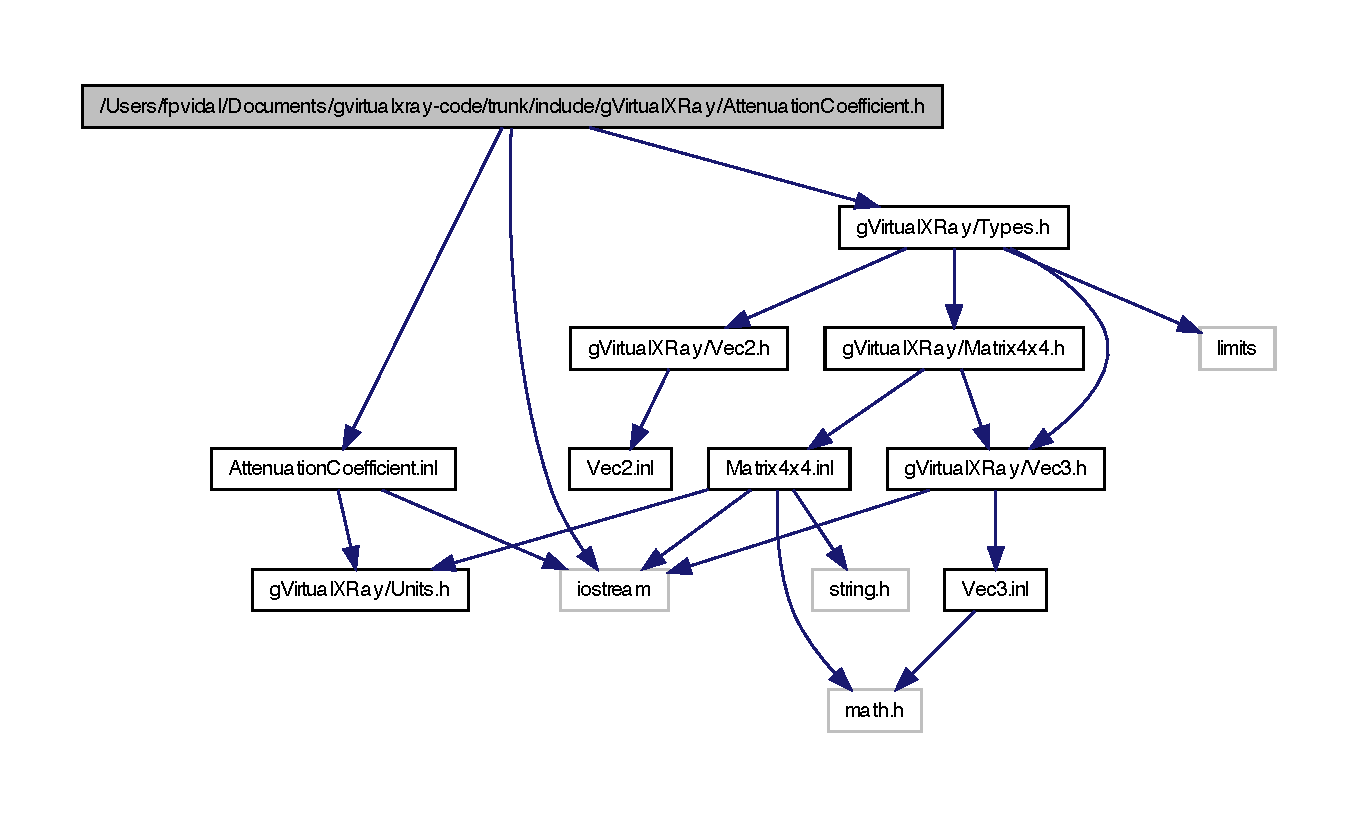
\includegraphics[width=400pt]{_attenuation_coefficient_8h__incl}
\end{center}
\end{figure}
This graph shows which files directly or indirectly include this file:\nopagebreak
\begin{figure}[H]
\begin{center}
\leavevmode
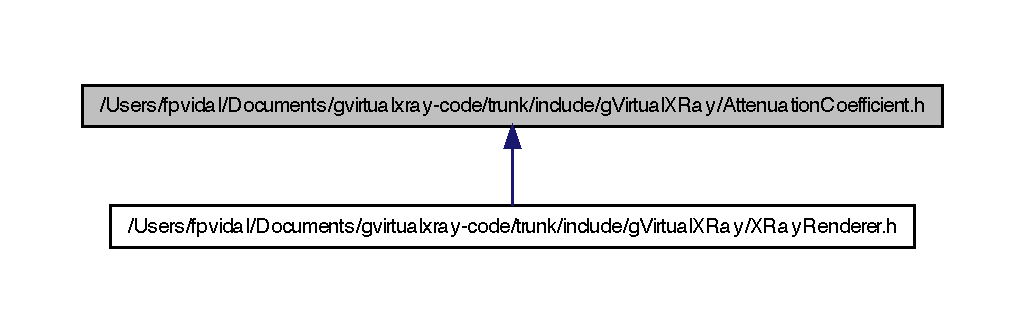
\includegraphics[width=400pt]{_attenuation_coefficient_8h__dep__incl}
\end{center}
\end{figure}
\subsection*{Classes}
\begin{DoxyCompactItemize}
\item 
class \hyperlink{classg_virtual_x_ray_1_1_attenuation_coefficient}{gVirtualXRay::AttenuationCoefficient}
\begin{DoxyCompactList}\small\item\em \hyperlink{classg_virtual_x_ray_1_1_attenuation_coefficient}{AttenuationCoefficient} is a class to handle an attenuation coefficient. \end{DoxyCompactList}\end{DoxyCompactItemize}
\subsection*{Namespaces}
\begin{DoxyCompactItemize}
\item 
namespace \hyperlink{namespaceg_virtual_x_ray}{gVirtualXRay}
\end{DoxyCompactItemize}
\subsection*{Functions}
\begin{DoxyCompactItemize}
\item 
std::istream \& \hyperlink{namespaceg_virtual_x_ray_a2546ba9b44c83b1c24d0f04c66a0bb44}{gVirtualXRay::operator$>$$>$} (std::istream \&is, AttenuationCoefficient \&obj)
\begin{DoxyCompactList}\small\item\em operator$>$$>$ \end{DoxyCompactList}\item 
std::ostream \& \hyperlink{namespaceg_virtual_x_ray_a8f1be85e5a75666c8b56213fc4e35990}{gVirtualXRay::operator$<$$<$} (std::ostream \&os, const AttenuationCoefficient \&obj)
\begin{DoxyCompactList}\small\item\em operator$<$$<$ \end{DoxyCompactList}\end{DoxyCompactItemize}


\subsection{Detailed Description}
Class to manage an attenuation coefficient. \begin{DoxyVersion}{Version}
1.0
\end{DoxyVersion}
\begin{DoxyDate}{Date}
30/11/2013
\end{DoxyDate}
\begin{DoxyAuthor}{Author}
Dr Franck P. Vidal
\end{DoxyAuthor}
\hypertarget{_x_ray_renderer_8inl_License}{}\subsection{License}\label{_x_ray_renderer_8inl_License}
BSD 3-\/Clause License.

For details on use and redistribution please refer to \href{http://opensource.org/licenses/BSD-3-Clause}{\tt http://opensource.org/licenses/BSD-\/3-\/Clause}\hypertarget{_x_ray_renderer_8inl_Copyright}{}\subsection{Copyright}\label{_x_ray_renderer_8inl_Copyright}
(c) by Dr Franck P. Vidal (\href{mailto:franck.p.vidal@fpvidal.net}{\tt franck.p.vidal@fpvidal.net}), \href{http://www.fpvidal.net/,}{\tt http://www.fpvidal.net/,} Dec 2013, 2013, version 1.0, BSD 3-\/Clause License 

Definition in file \hyperlink{_attenuation_coefficient_8h_source}{AttenuationCoefficient.h}.


\hypertarget{_attenuation_coefficient_8inl}{
\section{/Users/fpvidal/Documents/gvirtualxray-\/code/trunk/include/gVirtualXRay/AttenuationCoefficient.inl File Reference}
\label{_attenuation_coefficient_8inl}\index{/Users/fpvidal/Documents/gvirtualxray-\/code/trunk/include/gVirtualXRay/AttenuationCoefficient.inl@{/Users/fpvidal/Documents/gvirtualxray-\/code/trunk/include/gVirtualXRay/AttenuationCoefficient.inl}}
}


Class to manage an attenuation coefficient.  


{\ttfamily \#include $<$iostream$>$}\par
{\ttfamily \#include \char`\"{}gVirtualXRay/Units.h\char`\"{}}\par
Include dependency graph for AttenuationCoefficient.inl:\nopagebreak
\begin{figure}[H]
\begin{center}
\leavevmode
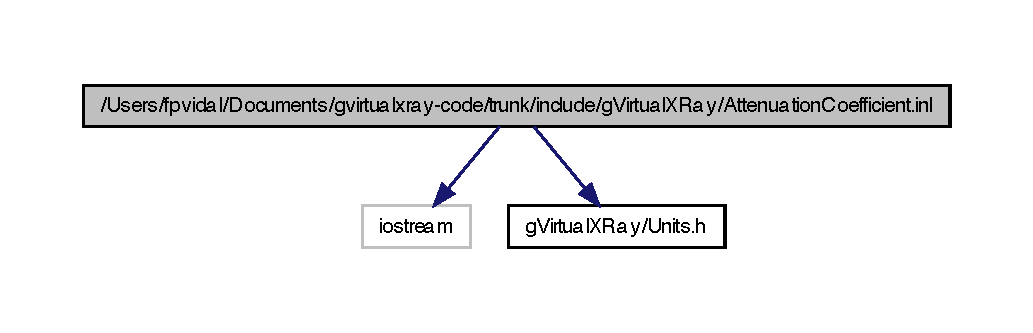
\includegraphics[width=400pt]{_attenuation_coefficient_8inl__incl}
\end{center}
\end{figure}
This graph shows which files directly or indirectly include this file:\nopagebreak
\begin{figure}[H]
\begin{center}
\leavevmode
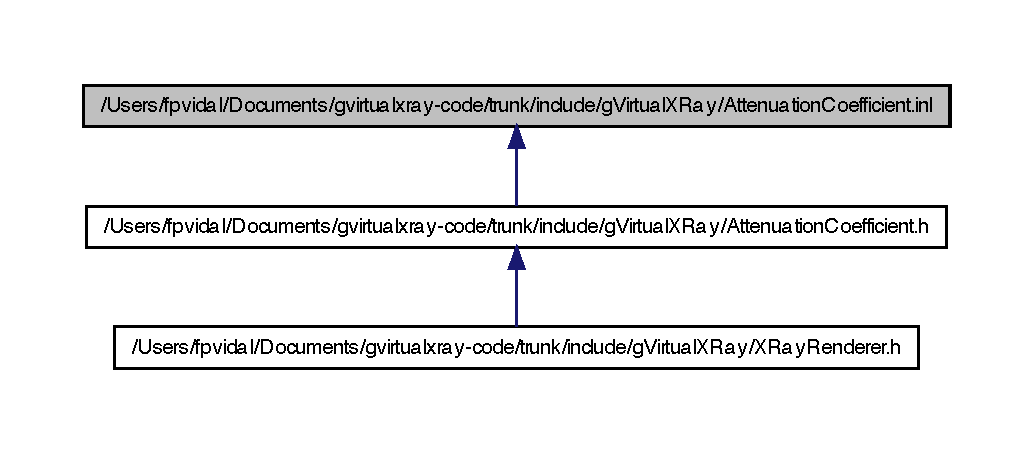
\includegraphics[width=400pt]{_attenuation_coefficient_8inl__dep__incl}
\end{center}
\end{figure}
\subsection*{Namespaces}
\begin{DoxyCompactItemize}
\item 
namespace \hyperlink{namespaceg_virtual_x_ray}{gVirtualXRay}
\end{DoxyCompactItemize}
\subsection*{Functions}
\begin{DoxyCompactItemize}
\item 
std::istream \& \hyperlink{namespaceg_virtual_x_ray_a2546ba9b44c83b1c24d0f04c66a0bb44}{gVirtualXRay::operator$>$$>$} (std::istream \&is, AttenuationCoefficient \&obj)
\begin{DoxyCompactList}\small\item\em operator$>$$>$ \end{DoxyCompactList}\item 
std::ostream \& \hyperlink{namespaceg_virtual_x_ray_a8f1be85e5a75666c8b56213fc4e35990}{gVirtualXRay::operator$<$$<$} (std::ostream \&os, const AttenuationCoefficient \&obj)
\begin{DoxyCompactList}\small\item\em operator$<$$<$ \end{DoxyCompactList}\end{DoxyCompactItemize}


\subsection{Detailed Description}
Class to manage an attenuation coefficient. \begin{DoxyVersion}{Version}
1.0
\end{DoxyVersion}
\begin{DoxyDate}{Date}
30/11/2013
\end{DoxyDate}
\begin{DoxyAuthor}{Author}
Dr Franck P. Vidal
\end{DoxyAuthor}
\hypertarget{_x_ray_renderer_8inl_License}{}\subsection{License}\label{_x_ray_renderer_8inl_License}
BSD 3-\/Clause License.

For details on use and redistribution please refer to \href{http://opensource.org/licenses/BSD-3-Clause}{\tt http://opensource.org/licenses/BSD-\/3-\/Clause}\hypertarget{_x_ray_renderer_8inl_Copyright}{}\subsection{Copyright}\label{_x_ray_renderer_8inl_Copyright}
(c) by Dr Franck P. Vidal (\href{mailto:franck.p.vidal@fpvidal.net}{\tt franck.p.vidal@fpvidal.net}), \href{http://www.fpvidal.net/,}{\tt http://www.fpvidal.net/,} Dec 2013, 2013, version 1.0, BSD 3-\/Clause License 

Definition in file \hyperlink{_attenuation_coefficient_8inl_source}{AttenuationCoefficient.inl}.


\hypertarget{_cube_mesh_8h}{
\section{/Users/fpvidal/Documents/gvirtualxray-\/code/trunk/include/gVirtualXRay/CubeMesh.h File Reference}
\label{_cube_mesh_8h}\index{/Users/fpvidal/Documents/gvirtualxray-\/code/trunk/include/gVirtualXRay/CubeMesh.h@{/Users/fpvidal/Documents/gvirtualxray-\/code/trunk/include/gVirtualXRay/CubeMesh.h}}
}


Class to handle 3D meshes of cubes.  


{\ttfamily \#include $<$string$>$}\par
{\ttfamily \#include $<$vector$>$}\par
{\ttfamily \#include \char`\"{}gVirtualXRay/PolygonMesh.h\char`\"{}}\par
{\ttfamily \#include \char`\"{}gVirtualXRay/Types.h\char`\"{}}\par
{\ttfamily \#include \char`\"{}CubeMesh.inl\char`\"{}}\par
Include dependency graph for CubeMesh.h:
\nopagebreak
\begin{figure}[H]
\begin{center}
\leavevmode
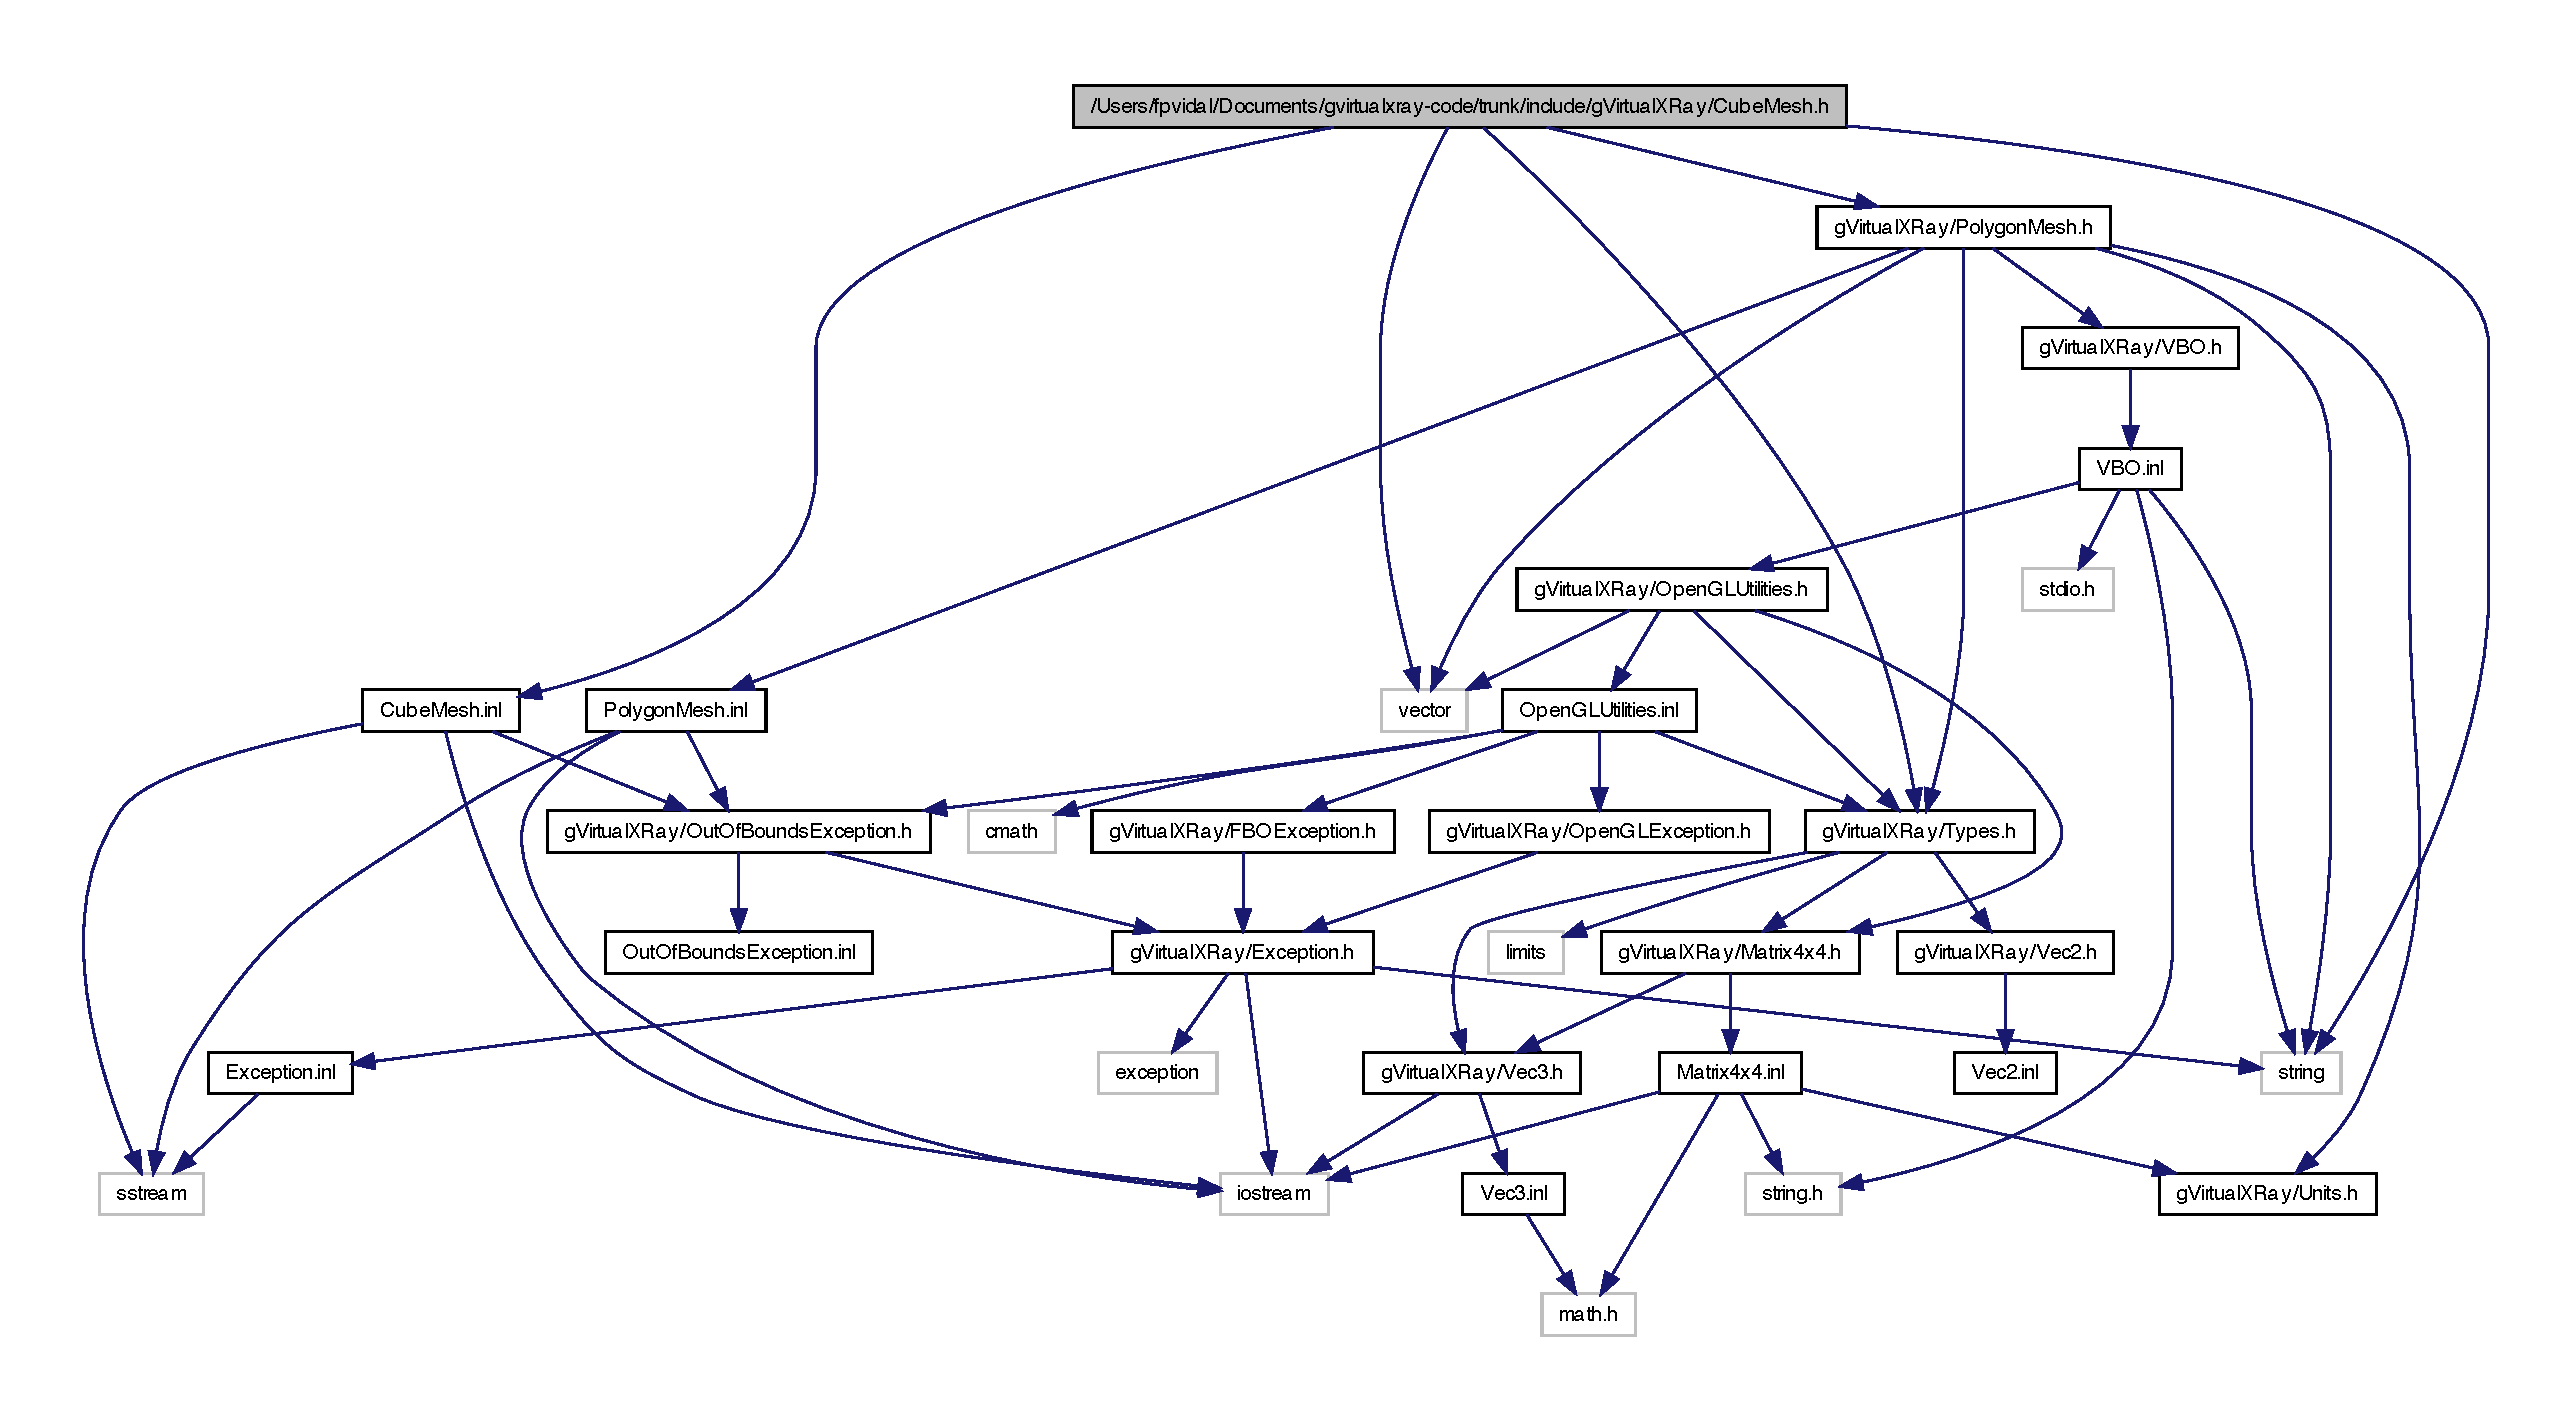
\includegraphics[width=400pt]{_cube_mesh_8h__incl}
\end{center}
\end{figure}
This graph shows which files directly or indirectly include this file:\nopagebreak
\begin{figure}[H]
\begin{center}
\leavevmode
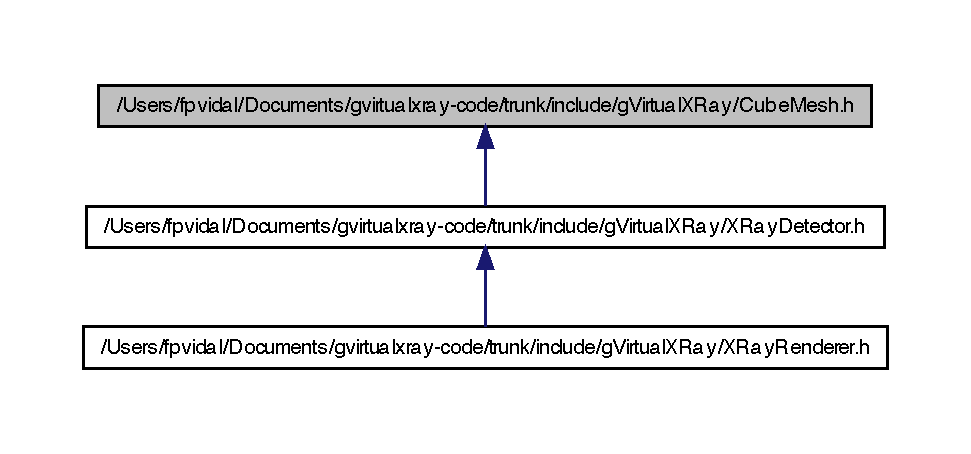
\includegraphics[width=400pt]{_cube_mesh_8h__dep__incl}
\end{center}
\end{figure}
\subsection*{Classes}
\begin{DoxyCompactItemize}
\item 
class \hyperlink{class_graphics_1_1_cube_mesh}{Graphics::CubeMesh}
\begin{DoxyCompactList}\small\item\em \hyperlink{class_graphics_1_1_cube_mesh}{CubeMesh} is a class to handle 3D meshes of cubes. \end{DoxyCompactList}\end{DoxyCompactItemize}
\subsection*{Namespaces}
\begin{DoxyCompactItemize}
\item 
namespace \hyperlink{namespace_graphics}{Graphics}
\end{DoxyCompactItemize}


\subsection{Detailed Description}
Class to handle 3D meshes of cubes. \begin{DoxyVersion}{Version}
1.0
\end{DoxyVersion}
\begin{DoxyDate}{Date}
23/03/2014
\end{DoxyDate}
\begin{DoxyAuthor}{Author}
Dr Franck P. Vidal
\end{DoxyAuthor}
\begin{Desc}
\item[\hyperlink{todo__todo000001}{Todo}]Make it possible to merge vertices if an array of indices exists\end{Desc}
\hypertarget{_x_ray_renderer_8inl_License}{}\subsection{License}\label{_x_ray_renderer_8inl_License}
BSD 3-\/Clause License.

For details on use and redistribution please refer to \href{http://opensource.org/licenses/BSD-3-Clause}{\tt http://opensource.org/licenses/BSD-\/3-\/Clause}\hypertarget{_x_ray_renderer_8inl_Copyright}{}\subsection{Copyright}\label{_x_ray_renderer_8inl_Copyright}
(c) by Dr Franck P. Vidal (\href{mailto:franck.p.vidal@fpvidal.net}{\tt franck.p.vidal@fpvidal.net}), \href{http://www.fpvidal.net/,}{\tt http://www.fpvidal.net/,} Dec 2013, 2013, version 1.0, BSD 3-\/Clause License 

Definition in file \hyperlink{_cube_mesh_8h_source}{CubeMesh.h}.


\hypertarget{_cube_mesh_8inl}{
\section{/Users/fpvidal/Documents/gvirtualxray-\/code/trunk/include/gVirtualXRay/CubeMesh.inl File Reference}
\label{_cube_mesh_8inl}\index{/Users/fpvidal/Documents/gvirtualxray-\/code/trunk/include/gVirtualXRay/CubeMesh.inl@{/Users/fpvidal/Documents/gvirtualxray-\/code/trunk/include/gVirtualXRay/CubeMesh.inl}}
}


Class to handle 3D meshes of cubes.  


{\ttfamily \#include $<$iostream$>$}\par
{\ttfamily \#include $<$sstream$>$}\par
{\ttfamily \#include \char`\"{}gVirtualXRay/OutOfBoundsException.h\char`\"{}}\par
Include dependency graph for CubeMesh.inl:\nopagebreak
\begin{figure}[H]
\begin{center}
\leavevmode
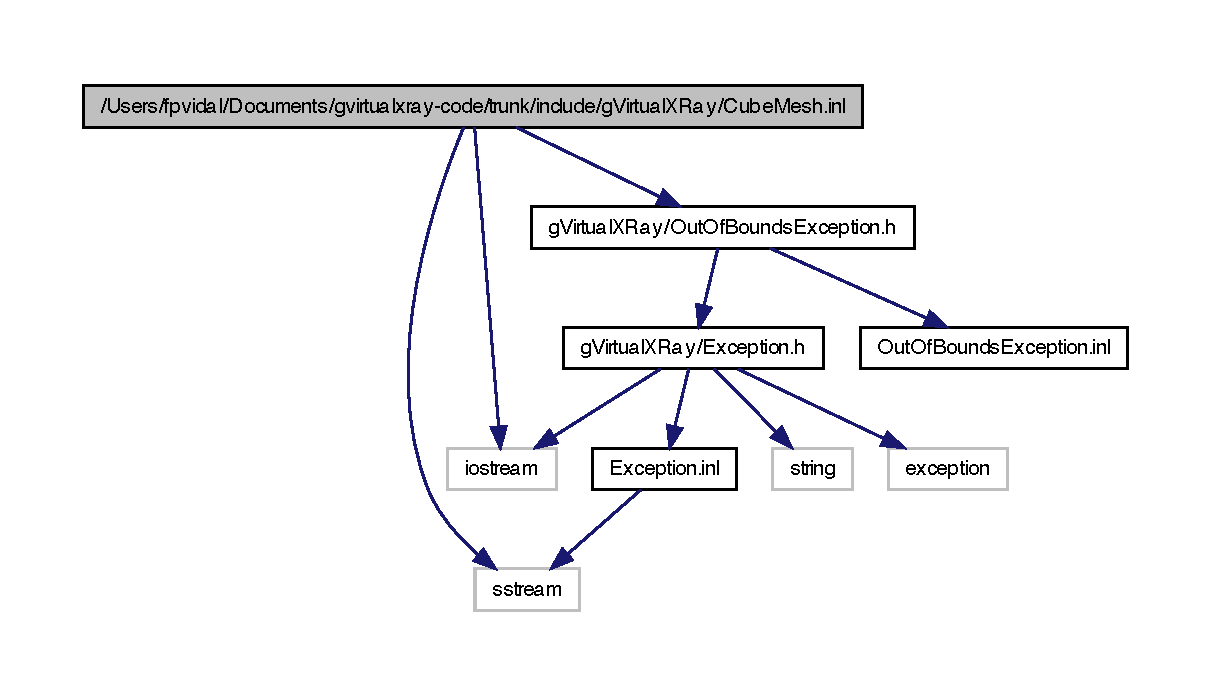
\includegraphics[width=400pt]{_cube_mesh_8inl__incl}
\end{center}
\end{figure}
This graph shows which files directly or indirectly include this file:\nopagebreak
\begin{figure}[H]
\begin{center}
\leavevmode
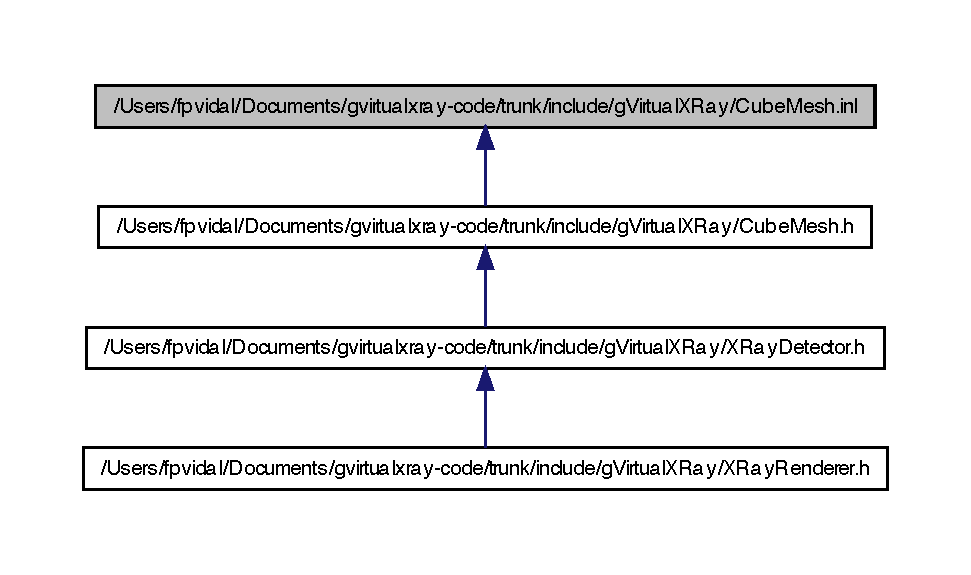
\includegraphics[width=400pt]{_cube_mesh_8inl__dep__incl}
\end{center}
\end{figure}
\subsection*{Namespaces}
\begin{DoxyCompactItemize}
\item 
namespace \hyperlink{namespace_graphics}{Graphics}
\end{DoxyCompactItemize}


\subsection{Detailed Description}
Class to handle 3D meshes of cubes. \begin{DoxyVersion}{Version}
1.0
\end{DoxyVersion}
\begin{DoxyDate}{Date}
23/03/2014
\end{DoxyDate}
\begin{DoxyAuthor}{Author}
Dr Franck P. Vidal
\end{DoxyAuthor}
\begin{Desc}
\item[\hyperlink{todo__todo000002}{Todo}]Make it possible to merge vertices if an array of indices exists\end{Desc}
\hypertarget{_x_ray_renderer_8inl_License}{}\subsection{License}\label{_x_ray_renderer_8inl_License}
BSD 3-\/Clause License.

For details on use and redistribution please refer to \href{http://opensource.org/licenses/BSD-3-Clause}{\tt http://opensource.org/licenses/BSD-\/3-\/Clause}\hypertarget{_x_ray_renderer_8inl_Copyright}{}\subsection{Copyright}\label{_x_ray_renderer_8inl_Copyright}
(c) by Dr Franck P. Vidal (\href{mailto:franck.p.vidal@fpvidal.net}{\tt franck.p.vidal@fpvidal.net}), \href{http://www.fpvidal.net/,}{\tt http://www.fpvidal.net/,} Dec 2013, 2013, version 1.0, BSD 3-\/Clause License 

Definition in file \hyperlink{_cube_mesh_8inl_source}{CubeMesh.inl}.


\hypertarget{_exception_8h}{
\section{/Users/fpvidal/Documents/gvirtualxray-\/code/trunk/include/gVirtualXRay/Exception.h File Reference}
\label{_exception_8h}\index{/Users/fpvidal/Documents/gvirtualxray-\/code/trunk/include/gVirtualXRay/Exception.h@{/Users/fpvidal/Documents/gvirtualxray-\/code/trunk/include/gVirtualXRay/Exception.h}}
}


Generic class to handle exceptions.  


{\ttfamily \#include $<$string$>$}\par
{\ttfamily \#include $<$exception$>$}\par
{\ttfamily \#include $<$iostream$>$}\par
{\ttfamily \#include \char`\"{}Exception.inl\char`\"{}}\par
Include dependency graph for Exception.h:\nopagebreak
\begin{figure}[H]
\begin{center}
\leavevmode
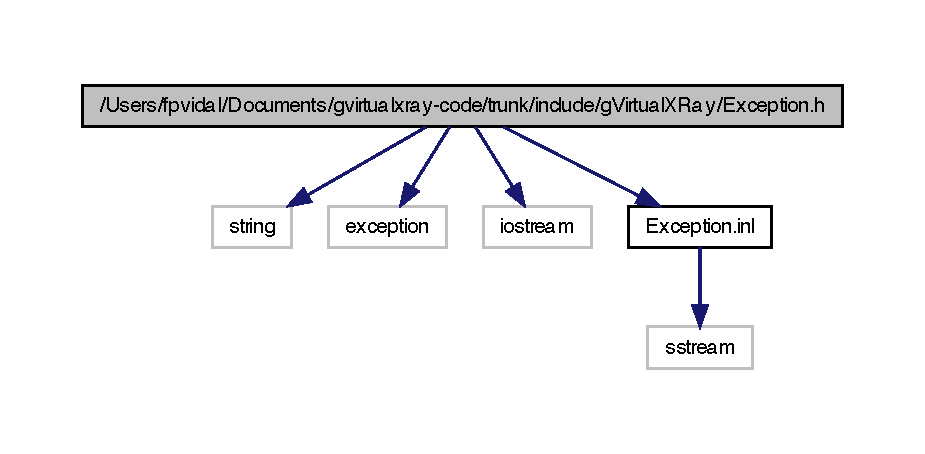
\includegraphics[width=400pt]{_exception_8h__incl}
\end{center}
\end{figure}
This graph shows which files directly or indirectly include this file:
\nopagebreak
\begin{figure}[H]
\begin{center}
\leavevmode
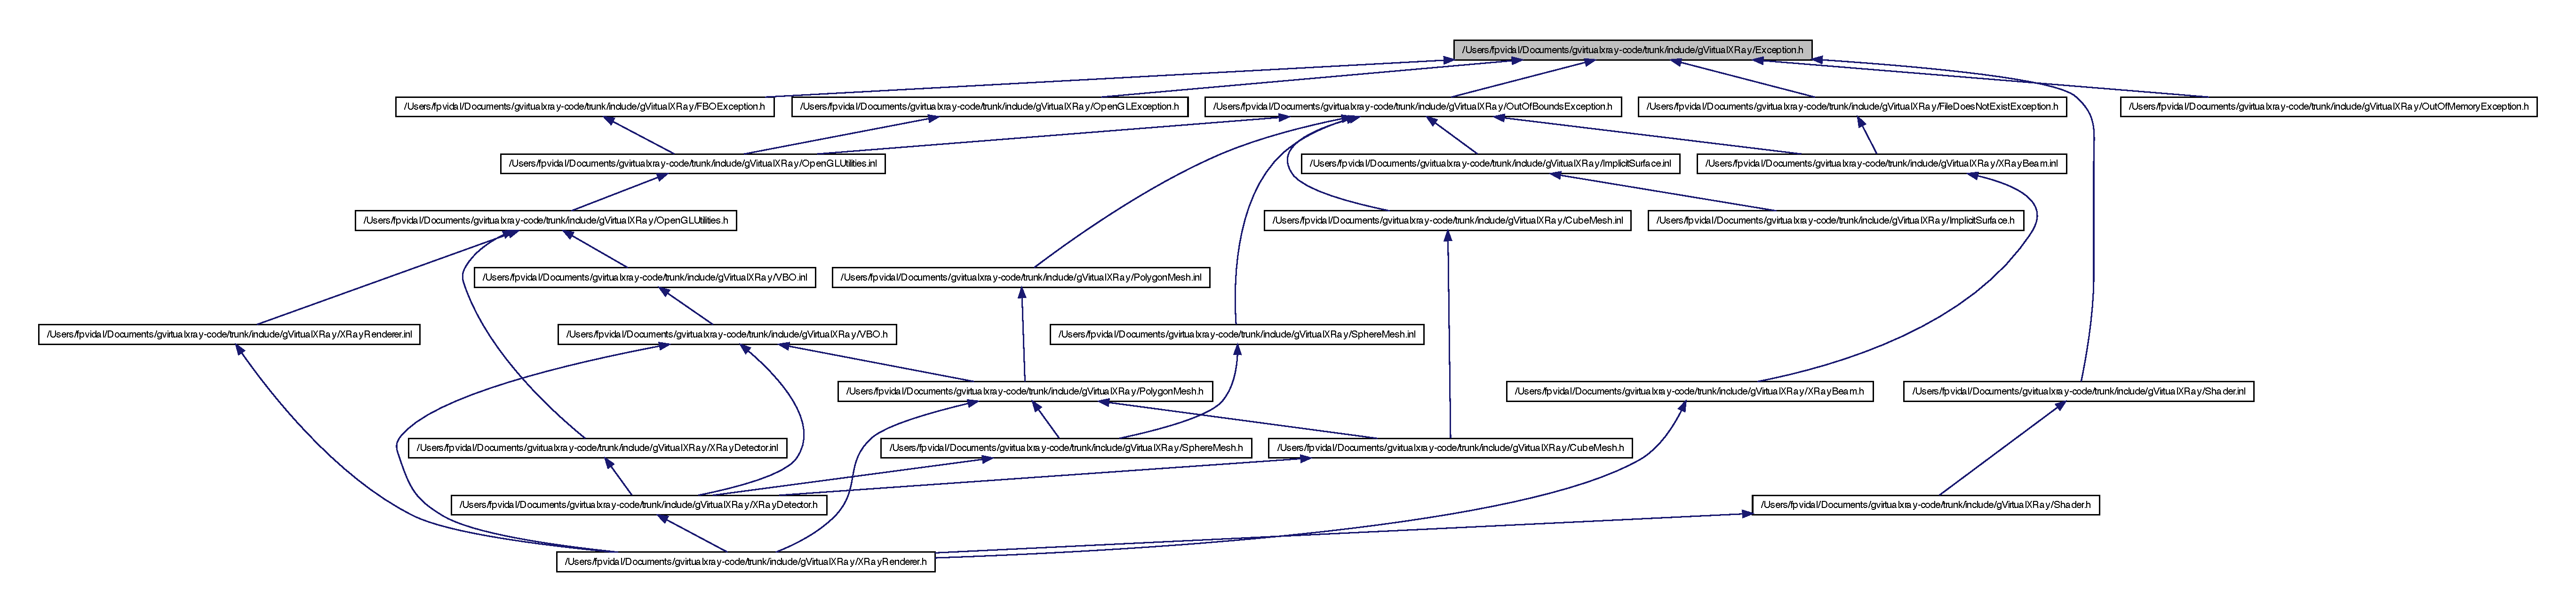
\includegraphics[width=400pt]{_exception_8h__dep__incl}
\end{center}
\end{figure}
\subsection*{Classes}
\begin{DoxyCompactItemize}
\item 
class \hyperlink{class_utilities_1_1_exception}{Utilities::Exception}
\begin{DoxyCompactList}\small\item\em \hyperlink{class_utilities_1_1_exception}{Exception} is a class to handle exceptions. \end{DoxyCompactList}\end{DoxyCompactItemize}
\subsection*{Namespaces}
\begin{DoxyCompactItemize}
\item 
namespace \hyperlink{namespace_utilities}{Utilities}
\end{DoxyCompactItemize}
\subsection*{Functions}
\begin{DoxyCompactItemize}
\item 
std::ostream \& \hyperlink{namespace_utilities_a1b36a6b137d8abe02a7f79072473e3b4}{Utilities::operator$<$$<$} (std::ostream \&anOutputStream, const Exception \&anException)
\begin{DoxyCompactList}\small\item\em operator$<$$<$ \end{DoxyCompactList}\end{DoxyCompactItemize}


\subsection{Detailed Description}
Generic class to handle exceptions. \begin{DoxyVersion}{Version}
1.0
\end{DoxyVersion}
\begin{DoxyDate}{Date}
07/11/2013
\end{DoxyDate}
\begin{DoxyAuthor}{Author}
Dr Franck P. Vidal
\end{DoxyAuthor}
\hypertarget{_x_ray_renderer_8inl_License}{}\subsection{License}\label{_x_ray_renderer_8inl_License}
BSD 3-\/Clause License.

For details on use and redistribution please refer to \href{http://opensource.org/licenses/BSD-3-Clause}{\tt http://opensource.org/licenses/BSD-\/3-\/Clause}\hypertarget{_x_ray_renderer_8inl_Copyright}{}\subsection{Copyright}\label{_x_ray_renderer_8inl_Copyright}
(c) by Dr Franck P. Vidal (\href{mailto:franck.p.vidal@fpvidal.net}{\tt franck.p.vidal@fpvidal.net}), \href{http://www.fpvidal.net/,}{\tt http://www.fpvidal.net/,} Dec 2013, 2013, version 1.0, BSD 3-\/Clause License 

Definition in file \hyperlink{_exception_8h_source}{Exception.h}.


\hypertarget{_exception_8inl}{
\section{/Users/fpvidal/Documents/gvirtualxray-\/code/trunk/include/gVirtualXRay/Exception.inl File Reference}
\label{_exception_8inl}\index{/Users/fpvidal/Documents/gvirtualxray-\/code/trunk/include/gVirtualXRay/Exception.inl@{/Users/fpvidal/Documents/gvirtualxray-\/code/trunk/include/gVirtualXRay/Exception.inl}}
}


Generic class to handle exceptions.  


{\ttfamily \#include $<$sstream$>$}\par
Include dependency graph for Exception.inl:\nopagebreak
\begin{figure}[H]
\begin{center}
\leavevmode
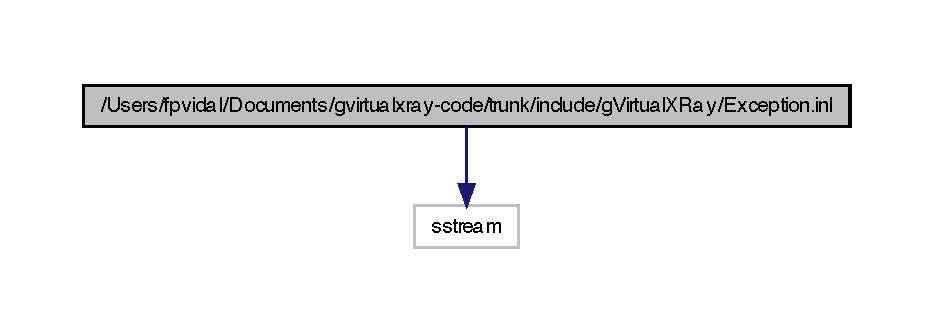
\includegraphics[width=400pt]{_exception_8inl__incl}
\end{center}
\end{figure}
This graph shows which files directly or indirectly include this file:
\nopagebreak
\begin{figure}[H]
\begin{center}
\leavevmode
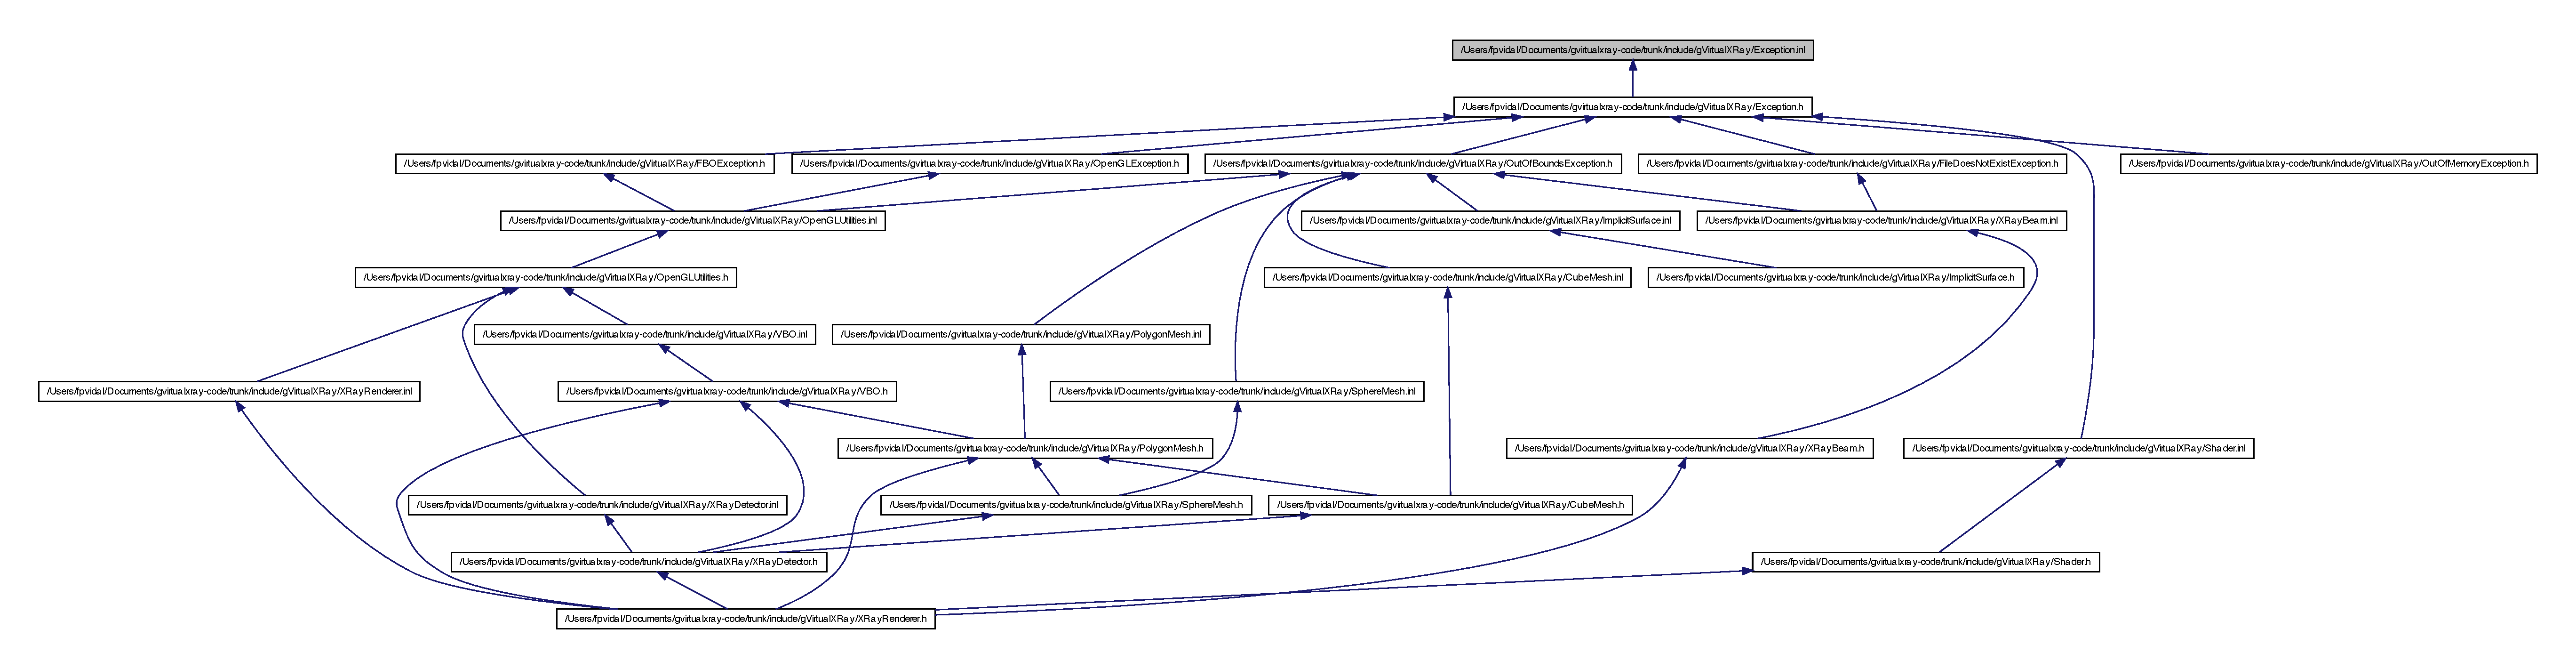
\includegraphics[width=400pt]{_exception_8inl__dep__incl}
\end{center}
\end{figure}
\subsection*{Namespaces}
\begin{DoxyCompactItemize}
\item 
namespace \hyperlink{namespace_utilities}{Utilities}
\end{DoxyCompactItemize}
\subsection*{Functions}
\begin{DoxyCompactItemize}
\item 
std::ostream \& \hyperlink{namespace_utilities_a1b36a6b137d8abe02a7f79072473e3b4}{Utilities::operator$<$$<$} (std::ostream \&anOutputStream, const Exception \&anException)
\begin{DoxyCompactList}\small\item\em operator$<$$<$ \end{DoxyCompactList}\end{DoxyCompactItemize}


\subsection{Detailed Description}
Generic class to handle exceptions. \begin{DoxyVersion}{Version}
1.0
\end{DoxyVersion}
\begin{DoxyDate}{Date}
07/11/2013
\end{DoxyDate}
\begin{DoxyAuthor}{Author}
Dr Franck P. Vidal
\end{DoxyAuthor}
\hypertarget{_x_ray_renderer_8inl_License}{}\subsection{License}\label{_x_ray_renderer_8inl_License}
BSD 3-\/Clause License.

For details on use and redistribution please refer to \href{http://opensource.org/licenses/BSD-3-Clause}{\tt http://opensource.org/licenses/BSD-\/3-\/Clause}\hypertarget{_x_ray_renderer_8inl_Copyright}{}\subsection{Copyright}\label{_x_ray_renderer_8inl_Copyright}
(c) by Dr Franck P. Vidal (\href{mailto:franck.p.vidal@fpvidal.net}{\tt franck.p.vidal@fpvidal.net}), \href{http://www.fpvidal.net/,}{\tt http://www.fpvidal.net/,} Dec 2013, 2013, version 1.0, BSD 3-\/Clause License 

Definition in file \hyperlink{_exception_8inl_source}{Exception.inl}.


\hypertarget{_f_b_o_exception_8h}{
\section{/Users/fpvidal/Documents/gvirtualxray-\/code/trunk/include/gVirtualXRay/FBOException.h File Reference}
\label{_f_b_o_exception_8h}\index{/Users/fpvidal/Documents/gvirtualxray-\/code/trunk/include/gVirtualXRay/FBOException.h@{/Users/fpvidal/Documents/gvirtualxray-\/code/trunk/include/gVirtualXRay/FBOException.h}}
}
{\ttfamily \#include \char`\"{}gVirtualXRay/Exception.h\char`\"{}}\par
Include dependency graph for FBOException.h:\nopagebreak
\begin{figure}[H]
\begin{center}
\leavevmode
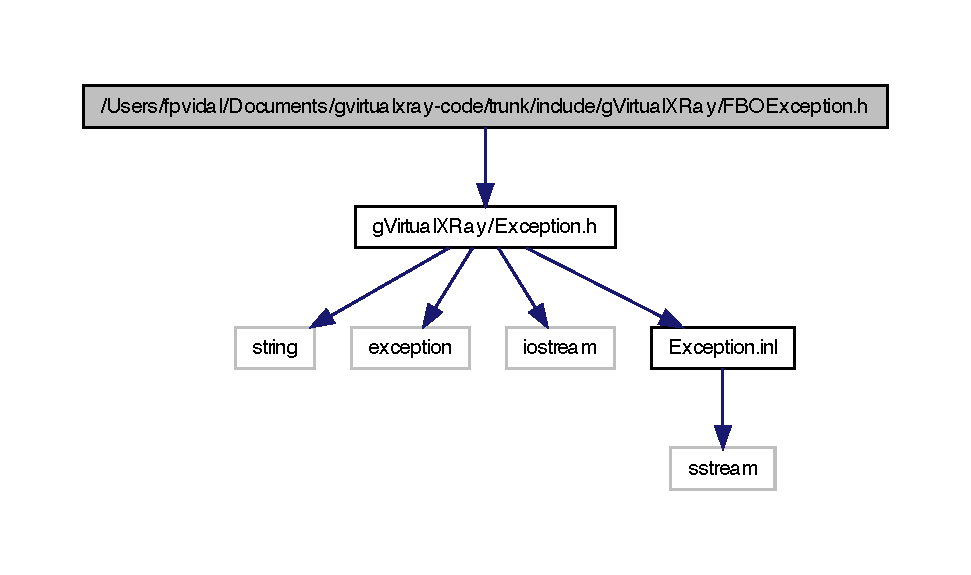
\includegraphics[width=400pt]{_f_b_o_exception_8h__incl}
\end{center}
\end{figure}
This graph shows which files directly or indirectly include this file:
\nopagebreak
\begin{figure}[H]
\begin{center}
\leavevmode
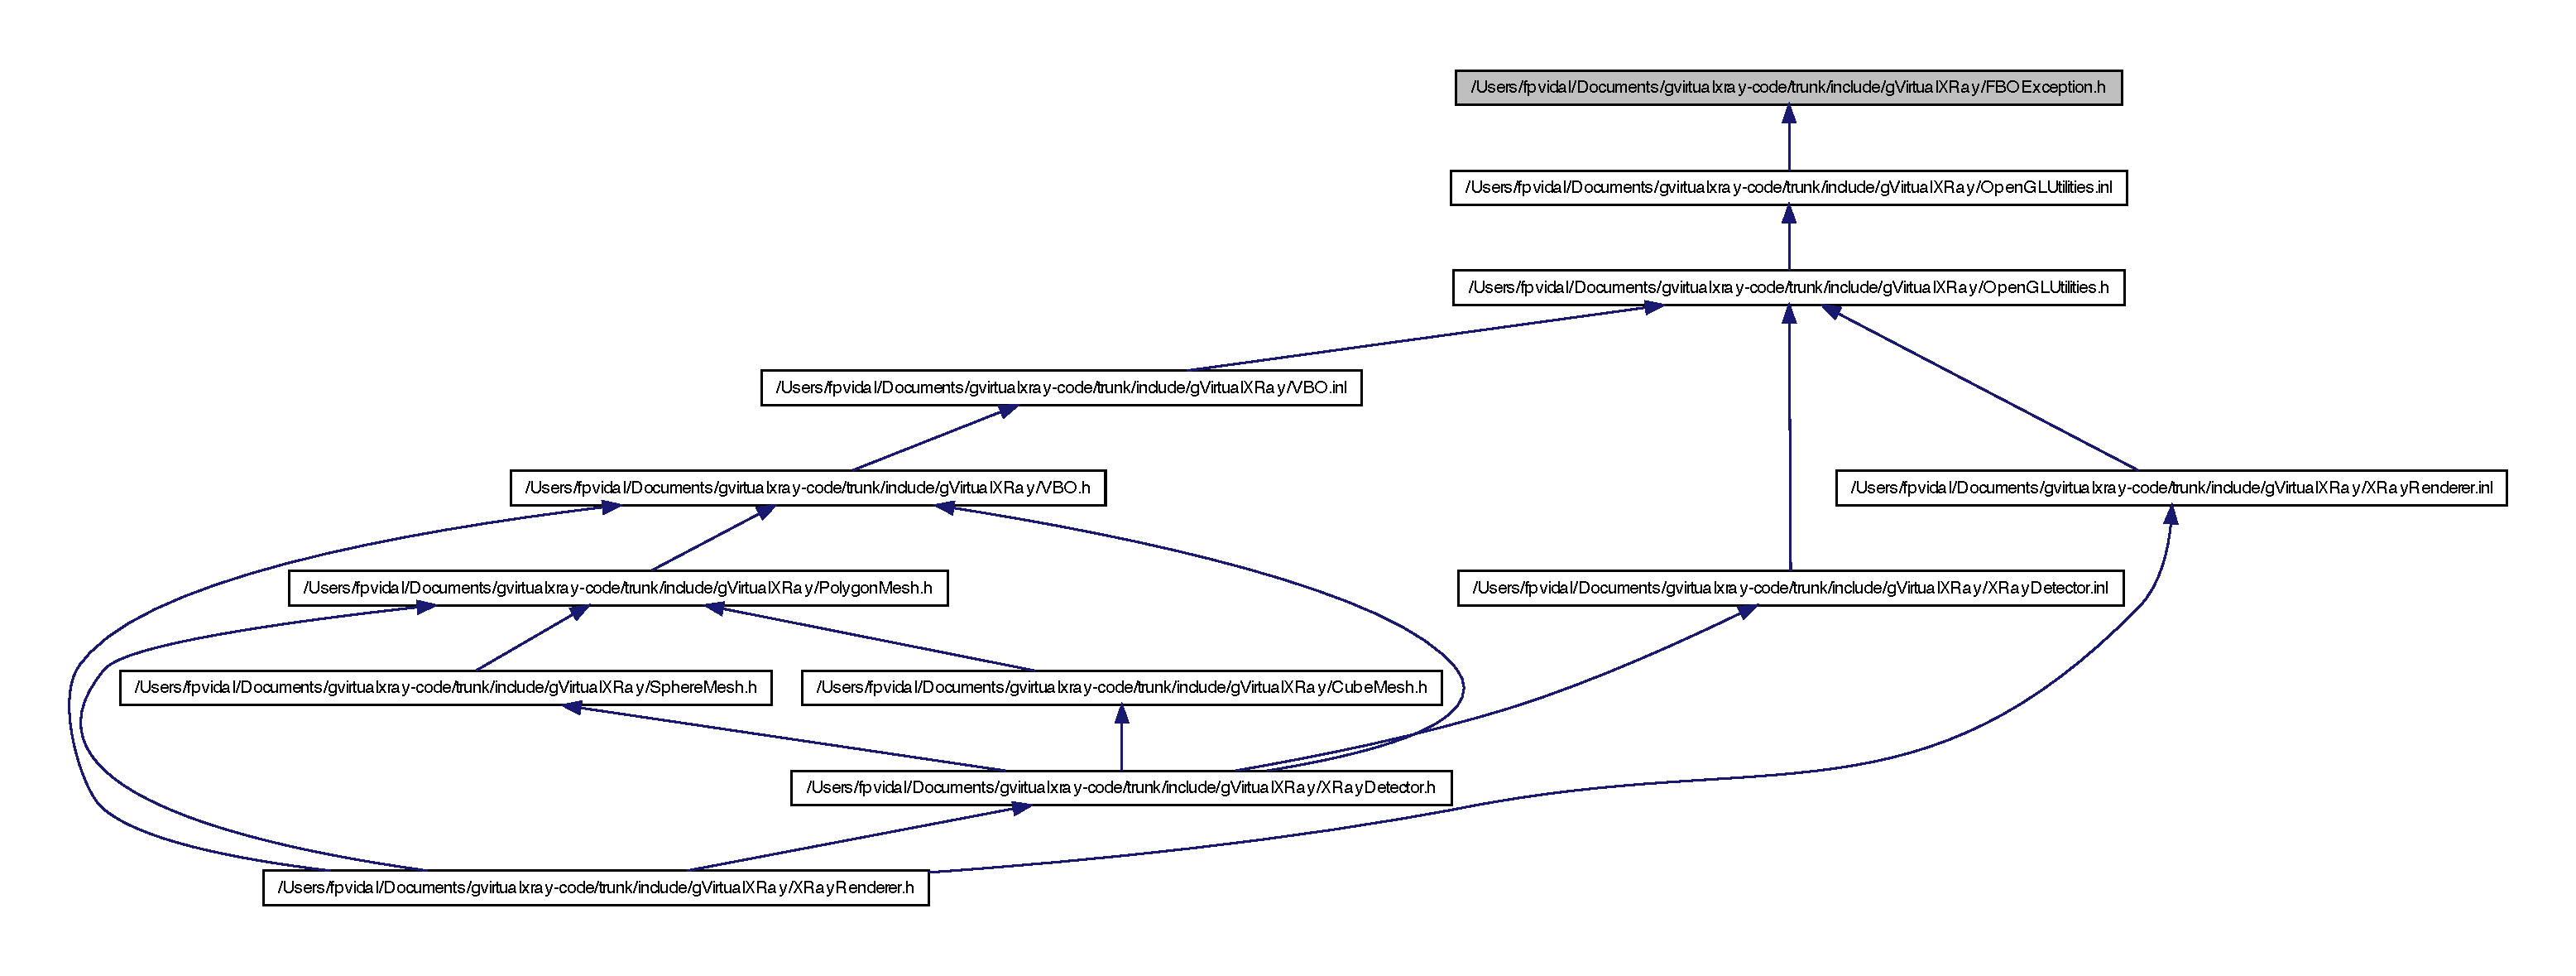
\includegraphics[width=400pt]{_f_b_o_exception_8h__dep__incl}
\end{center}
\end{figure}
\subsection*{Classes}
\begin{DoxyCompactItemize}
\item 
class \hyperlink{class_utilities_1_1_f_b_o_exception}{Utilities::FBOException}
\begin{DoxyCompactList}\small\item\em \hyperlink{class_utilities_1_1_f_b_o_exception}{FBOException} is a class to handle exceptions related to FBOs. \end{DoxyCompactList}\end{DoxyCompactItemize}
\subsection*{Namespaces}
\begin{DoxyCompactItemize}
\item 
namespace \hyperlink{namespace_utilities}{Utilities}
\end{DoxyCompactItemize}

\hypertarget{_file_does_not_exist_exception_8h}{
\section{/Users/fpvidal/Documents/gvirtualxray-\/code/trunk/include/gVirtualXRay/FileDoesNotExistException.h File Reference}
\label{_file_does_not_exist_exception_8h}\index{/Users/fpvidal/Documents/gvirtualxray-\/code/trunk/include/gVirtualXRay/FileDoesNotExistException.h@{/Users/fpvidal/Documents/gvirtualxray-\/code/trunk/include/gVirtualXRay/FileDoesNotExistException.h}}
}
{\ttfamily \#include $<$string$>$}\par
{\ttfamily \#include \char`\"{}gVirtualXRay/Exception.h\char`\"{}}\par
{\ttfamily \#include \char`\"{}FileDoesNotExistException.inl\char`\"{}}\par
Include dependency graph for FileDoesNotExistException.h:\nopagebreak
\begin{figure}[H]
\begin{center}
\leavevmode
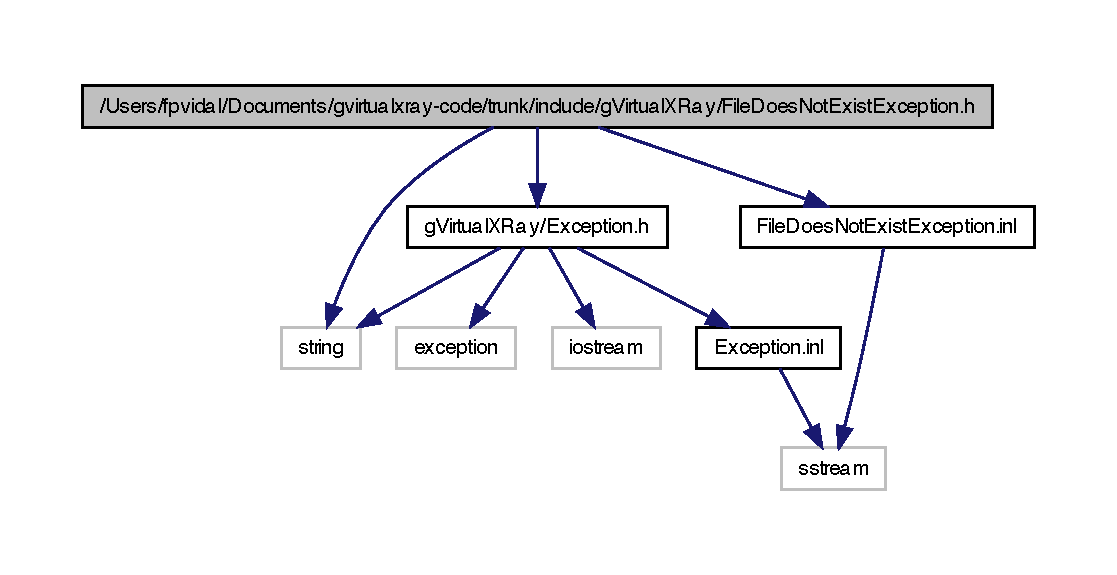
\includegraphics[width=400pt]{_file_does_not_exist_exception_8h__incl}
\end{center}
\end{figure}
This graph shows which files directly or indirectly include this file:\nopagebreak
\begin{figure}[H]
\begin{center}
\leavevmode
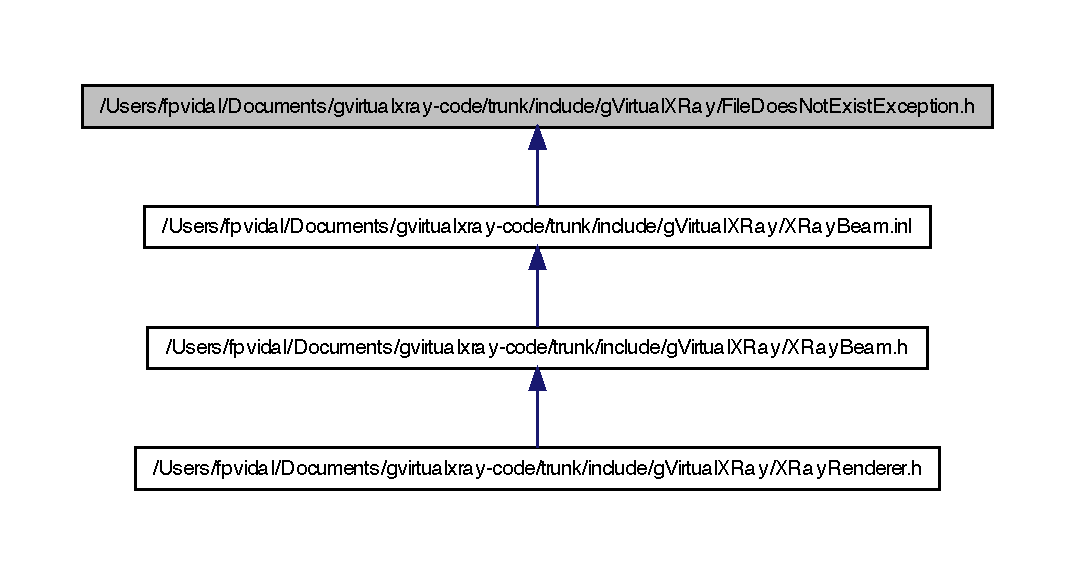
\includegraphics[width=400pt]{_file_does_not_exist_exception_8h__dep__incl}
\end{center}
\end{figure}
\subsection*{Classes}
\begin{DoxyCompactItemize}
\item 
class \hyperlink{class_utilities_1_1_file_does_not_exist_exception}{Utilities::FileDoesNotExistException}
\begin{DoxyCompactList}\small\item\em \hyperlink{class_utilities_1_1_file_does_not_exist_exception}{FileDoesNotExistException} is a class to handle exceptions when trying to open a read-\/only file that is not accessible. \end{DoxyCompactList}\end{DoxyCompactItemize}
\subsection*{Namespaces}
\begin{DoxyCompactItemize}
\item 
namespace \hyperlink{namespace_utilities}{Utilities}
\end{DoxyCompactItemize}

\hypertarget{_file_does_not_exist_exception_8inl}{
\section{/Users/fpvidal/Documents/gvirtualxray-\/code/trunk/include/gVirtualXRay/FileDoesNotExistException.inl File Reference}
\label{_file_does_not_exist_exception_8inl}\index{/Users/fpvidal/Documents/gvirtualxray-\/code/trunk/include/gVirtualXRay/FileDoesNotExistException.inl@{/Users/fpvidal/Documents/gvirtualxray-\/code/trunk/include/gVirtualXRay/FileDoesNotExistException.inl}}
}


Class to handle exceptions when trying to open a read-\/only file that is not accessible.  


{\ttfamily \#include $<$sstream$>$}\par
Include dependency graph for FileDoesNotExistException.inl:\nopagebreak
\begin{figure}[H]
\begin{center}
\leavevmode
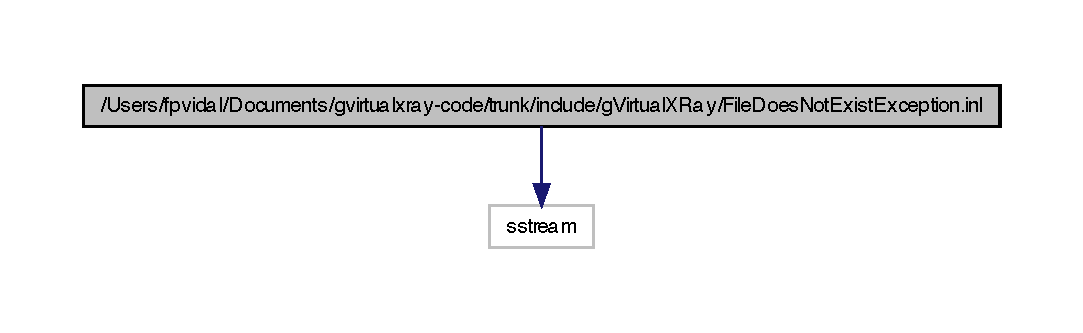
\includegraphics[width=400pt]{_file_does_not_exist_exception_8inl__incl}
\end{center}
\end{figure}
This graph shows which files directly or indirectly include this file:\nopagebreak
\begin{figure}[H]
\begin{center}
\leavevmode
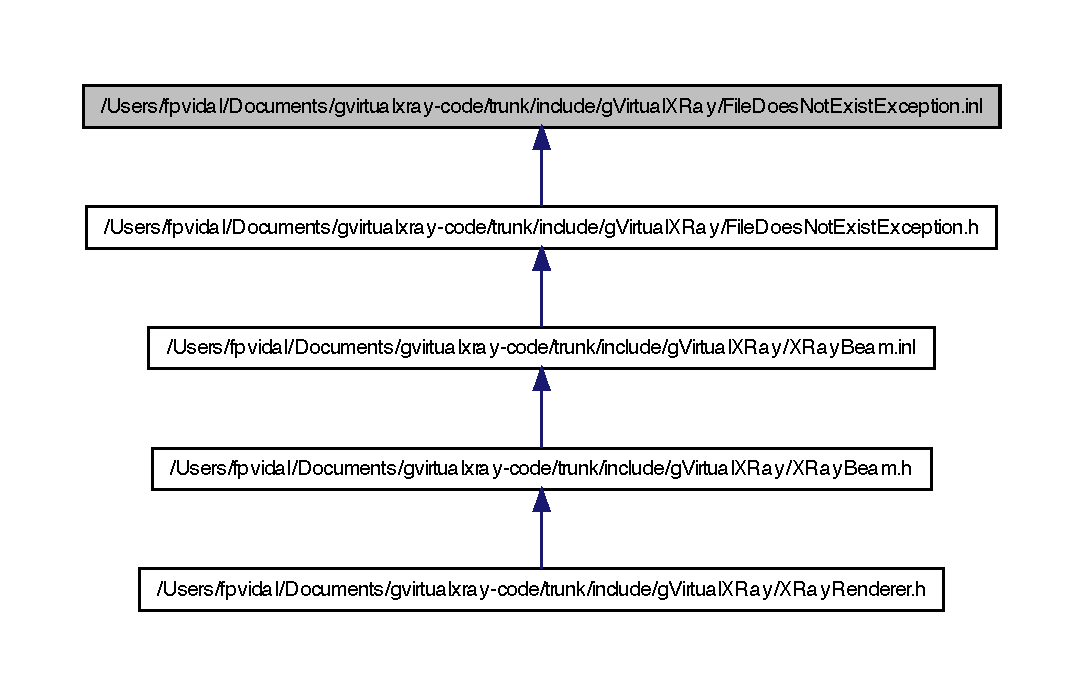
\includegraphics[width=400pt]{_file_does_not_exist_exception_8inl__dep__incl}
\end{center}
\end{figure}
\subsection*{Namespaces}
\begin{DoxyCompactItemize}
\item 
namespace \hyperlink{namespace_utilities}{Utilities}
\end{DoxyCompactItemize}


\subsection{Detailed Description}
Class to handle exceptions when trying to open a read-\/only file that is not accessible. \begin{DoxyVersion}{Version}
1.0
\end{DoxyVersion}
\begin{DoxyDate}{Date}
30/11/2013
\end{DoxyDate}
\begin{DoxyAuthor}{Author}
Dr Franck P. Vidal
\end{DoxyAuthor}
\hypertarget{_x_ray_renderer_8inl_License}{}\subsection{License}\label{_x_ray_renderer_8inl_License}
BSD 3-\/Clause License.

For details on use and redistribution please refer to \href{http://opensource.org/licenses/BSD-3-Clause}{\tt http://opensource.org/licenses/BSD-\/3-\/Clause}\hypertarget{_x_ray_renderer_8inl_Copyright}{}\subsection{Copyright}\label{_x_ray_renderer_8inl_Copyright}
(c) by Dr Franck P. Vidal (\href{mailto:franck.p.vidal@fpvidal.net}{\tt franck.p.vidal@fpvidal.net}), \href{http://www.fpvidal.net/,}{\tt http://www.fpvidal.net/,} Dec 2013, 2013, version 1.0, BSD 3-\/Clause License 

Definition in file \hyperlink{_file_does_not_exist_exception_8inl_source}{FileDoesNotExistException.inl}.


\hypertarget{framebuffer_object_8h}{
\section{/Users/fpvidal/Documents/gvirtualxray-\/code/trunk/include/gVirtualXRay/framebufferObject.h File Reference}
\label{framebuffer_object_8h}\index{/Users/fpvidal/Documents/gvirtualxray-\/code/trunk/include/gVirtualXRay/framebufferObject.h@{/Users/fpvidal/Documents/gvirtualxray-\/code/trunk/include/gVirtualXRay/framebufferObject.h}}
}
{\ttfamily \#include $<$GL/glew.h$>$}\par
{\ttfamily \#include $<$iostream$>$}\par
Include dependency graph for framebufferObject.h:\nopagebreak
\begin{figure}[H]
\begin{center}
\leavevmode
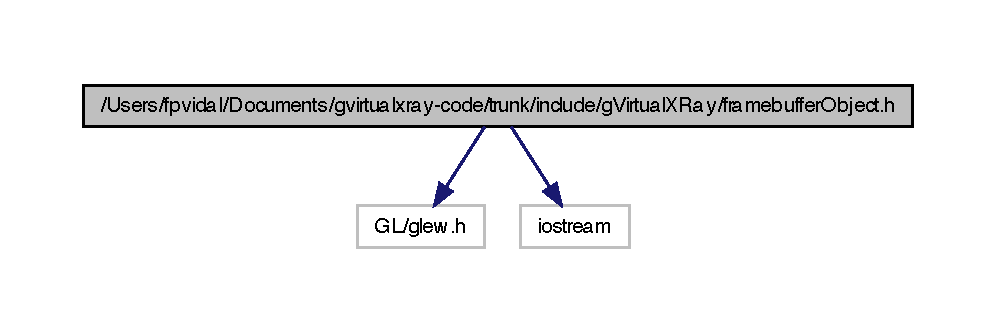
\includegraphics[width=400pt]{framebuffer_object_8h__incl}
\end{center}
\end{figure}
\subsection*{Classes}
\begin{DoxyCompactItemize}
\item 
class \hyperlink{class_framebuffer_object}{FramebufferObject}
\end{DoxyCompactItemize}

\hypertarget{_implicit_surface_8h}{
\section{/Users/fpvidal/Documents/gvirtualxray-\/code/trunk/include/gVirtualXRay/ImplicitSurface.h File Reference}
\label{_implicit_surface_8h}\index{/Users/fpvidal/Documents/gvirtualxray-\/code/trunk/include/gVirtualXRay/ImplicitSurface.h@{/Users/fpvidal/Documents/gvirtualxray-\/code/trunk/include/gVirtualXRay/ImplicitSurface.h}}
}


Class to build 3D implicit surfaces. To know what implicit surfaces are, please visit Paul Bourke's tutorial available at \href{http://paulbourke.net/geometry/implicitsurf/.}{\tt http://paulbourke.net/geometry/implicitsurf/.}  


{\ttfamily \#include $<$vector$>$}\par
{\ttfamily \#include \char`\"{}gVirtualXRay/Types.h\char`\"{}}\par
{\ttfamily \#include \char`\"{}ImplicitSurface.inl\char`\"{}}\par
Include dependency graph for ImplicitSurface.h:\nopagebreak
\begin{figure}[H]
\begin{center}
\leavevmode
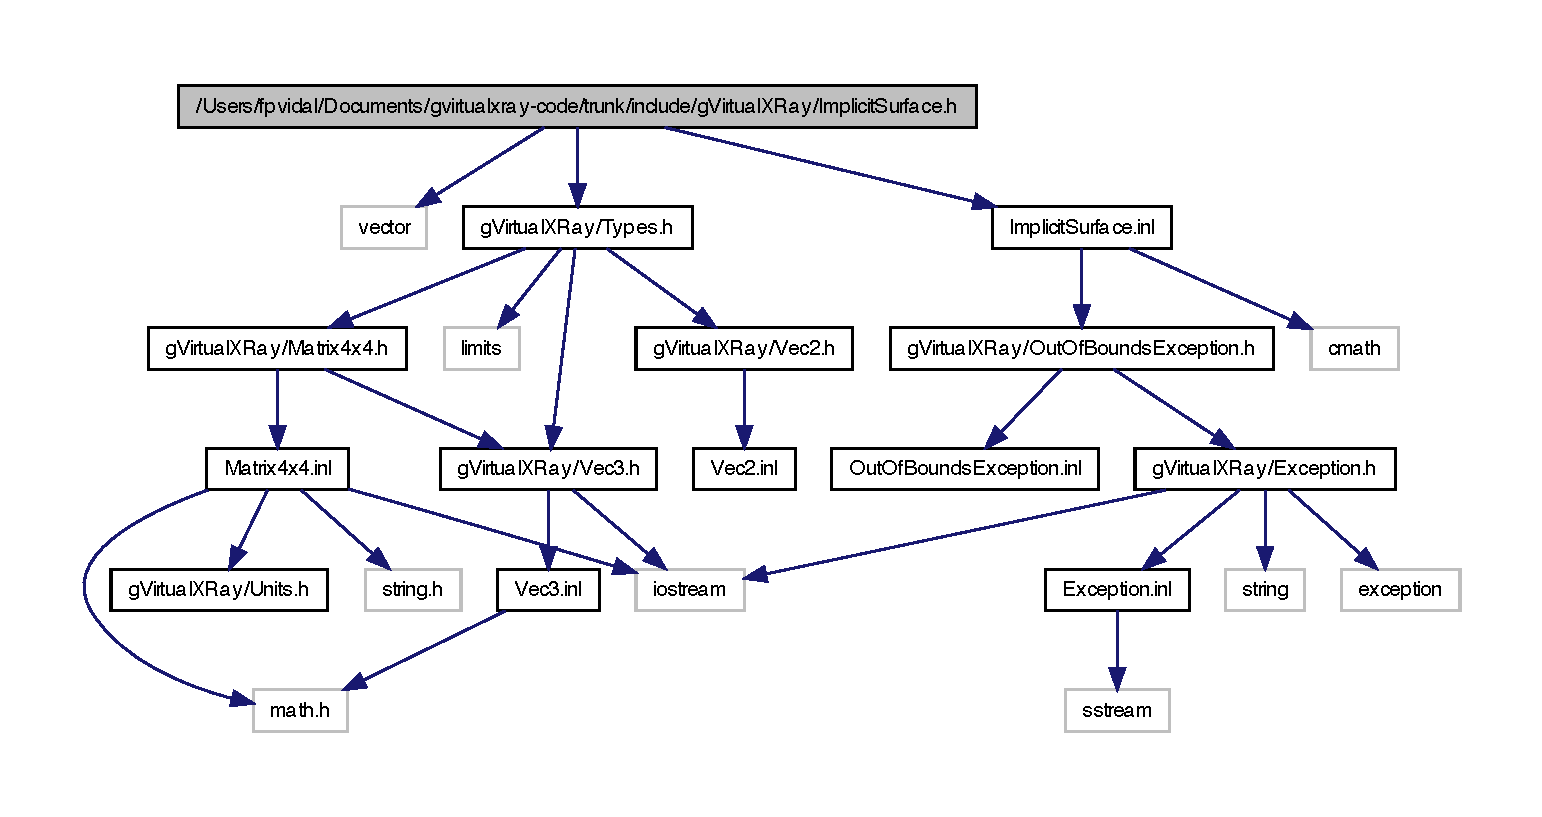
\includegraphics[width=400pt]{_implicit_surface_8h__incl}
\end{center}
\end{figure}
\subsection*{Classes}
\begin{DoxyCompactItemize}
\item 
class \hyperlink{class_graphics_1_1_implicit_surface}{Graphics::ImplicitSurface}
\begin{DoxyCompactList}\small\item\em \hyperlink{class_graphics_1_1_implicit_surface}{ImplicitSurface} is a class to build 3D implicit surfaces. \end{DoxyCompactList}\item 
class \hyperlink{class_graphics_1_1_implicit_surface_1_1_density_function_parameter_type}{Graphics::ImplicitSurface::DensityFunctionParameterType}
\begin{DoxyCompactList}\small\item\em Type of density function parameter. \end{DoxyCompactList}\end{DoxyCompactItemize}
\subsection*{Namespaces}
\begin{DoxyCompactItemize}
\item 
namespace \hyperlink{namespace_graphics}{Graphics}
\end{DoxyCompactItemize}


\subsection{Detailed Description}
Class to build 3D implicit surfaces. To know what implicit surfaces are, please visit Paul Bourke's tutorial available at \href{http://paulbourke.net/geometry/implicitsurf/.}{\tt http://paulbourke.net/geometry/implicitsurf/.} \begin{DoxyVersion}{Version}
1.0
\end{DoxyVersion}
\begin{DoxyDate}{Date}
08/03/2014
\end{DoxyDate}
\begin{DoxyAuthor}{Author}
Dr Franck P. Vidal
\end{DoxyAuthor}
\hypertarget{_x_ray_renderer_8inl_License}{}\subsection{License}\label{_x_ray_renderer_8inl_License}
BSD 3-\/Clause License.

For details on use and redistribution please refer to \href{http://opensource.org/licenses/BSD-3-Clause}{\tt http://opensource.org/licenses/BSD-\/3-\/Clause}\hypertarget{_x_ray_renderer_8inl_Copyright}{}\subsection{Copyright}\label{_x_ray_renderer_8inl_Copyright}
(c) by Dr Franck P. Vidal (\href{mailto:franck.p.vidal@fpvidal.net}{\tt franck.p.vidal@fpvidal.net}), \href{http://www.fpvidal.net/,}{\tt http://www.fpvidal.net/,} Dec 2013, 2013, version 1.0, BSD 3-\/Clause License 

Definition in file \hyperlink{_implicit_surface_8h_source}{ImplicitSurface.h}.


\hypertarget{_implicit_surface_8inl}{
\section{/Users/fpvidal/Documents/gvirtualxray-\/code/trunk/include/gVirtualXRay/ImplicitSurface.inl File Reference}
\label{_implicit_surface_8inl}\index{/Users/fpvidal/Documents/gvirtualxray-\/code/trunk/include/gVirtualXRay/ImplicitSurface.inl@{/Users/fpvidal/Documents/gvirtualxray-\/code/trunk/include/gVirtualXRay/ImplicitSurface.inl}}
}


Class to build 3D implicit surfaces. To know what implicit surfaces are, please visit Paul Bourke's tutorial available at \href{http://paulbourke.net/geometry/implicitsurf/.}{\tt http://paulbourke.net/geometry/implicitsurf/.}  


{\ttfamily \#include $<$cmath$>$}\par
{\ttfamily \#include \char`\"{}gVirtualXRay/OutOfBoundsException.h\char`\"{}}\par
Include dependency graph for ImplicitSurface.inl:\nopagebreak
\begin{figure}[H]
\begin{center}
\leavevmode
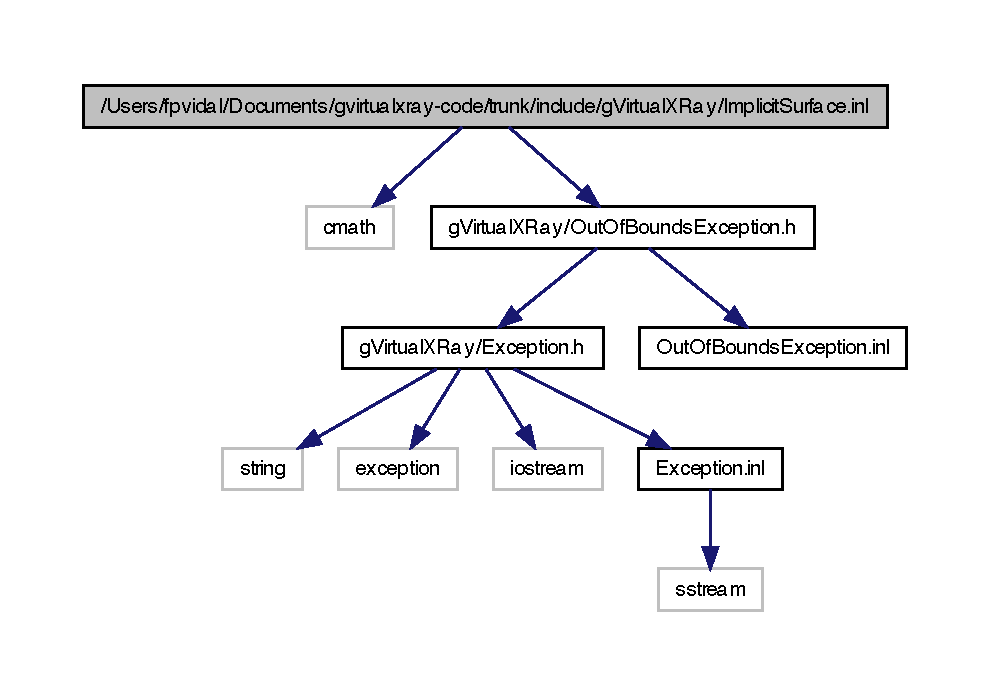
\includegraphics[width=400pt]{_implicit_surface_8inl__incl}
\end{center}
\end{figure}
This graph shows which files directly or indirectly include this file:\nopagebreak
\begin{figure}[H]
\begin{center}
\leavevmode
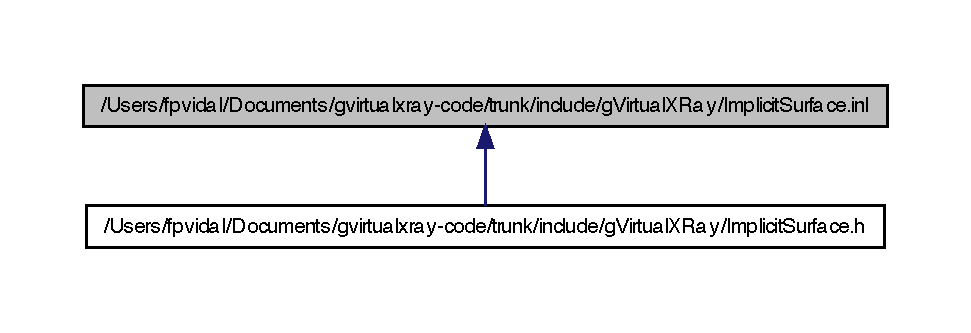
\includegraphics[width=400pt]{_implicit_surface_8inl__dep__incl}
\end{center}
\end{figure}
\subsection*{Namespaces}
\begin{DoxyCompactItemize}
\item 
namespace \hyperlink{namespace_graphics}{Graphics}
\end{DoxyCompactItemize}


\subsection{Detailed Description}
Class to build 3D implicit surfaces. To know what implicit surfaces are, please visit Paul Bourke's tutorial available at \href{http://paulbourke.net/geometry/implicitsurf/.}{\tt http://paulbourke.net/geometry/implicitsurf/.} \begin{DoxyVersion}{Version}
1.0
\end{DoxyVersion}
\begin{DoxyDate}{Date}
08/03/2014
\end{DoxyDate}
\begin{DoxyAuthor}{Author}
Dr Franck P. Vidal

Dr Franck P. Vidal
\end{DoxyAuthor}
\hypertarget{_x_ray_renderer_8inl_License}{}\subsection{License}\label{_x_ray_renderer_8inl_License}
BSD 3-\/Clause License.

For details on use and redistribution please refer to \href{http://opensource.org/licenses/BSD-3-Clause}{\tt http://opensource.org/licenses/BSD-\/3-\/Clause}\hypertarget{_x_ray_renderer_8inl_Copyright}{}\subsection{Copyright}\label{_x_ray_renderer_8inl_Copyright}
(c) by Dr Franck P. Vidal (\href{mailto:franck.p.vidal@fpvidal.net}{\tt franck.p.vidal@fpvidal.net}), \href{http://www.fpvidal.net/,}{\tt http://www.fpvidal.net/,} Dec 2013, 2013, version 1.0, BSD 3-\/Clause License 

Definition in file \hyperlink{_implicit_surface_8inl_source}{ImplicitSurface.inl}.


\hypertarget{_matrix4x4_8h}{
\section{/Users/fpvidal/Documents/gvirtualxray-\/code/trunk/include/gVirtualXRay/Matrix4x4.h File Reference}
\label{_matrix4x4_8h}\index{/Users/fpvidal/Documents/gvirtualxray-\/code/trunk/include/gVirtualXRay/Matrix4x4.h@{/Users/fpvidal/Documents/gvirtualxray-\/code/trunk/include/gVirtualXRay/Matrix4x4.h}}
}


Template class to handle a 4x4 matrixs.  


{\ttfamily \#include \char`\"{}gVirtualXRay/Vec3.h\char`\"{}}\par
{\ttfamily \#include \char`\"{}Matrix4x4.inl\char`\"{}}\par
Include dependency graph for Matrix4x4.h:\nopagebreak
\begin{figure}[H]
\begin{center}
\leavevmode
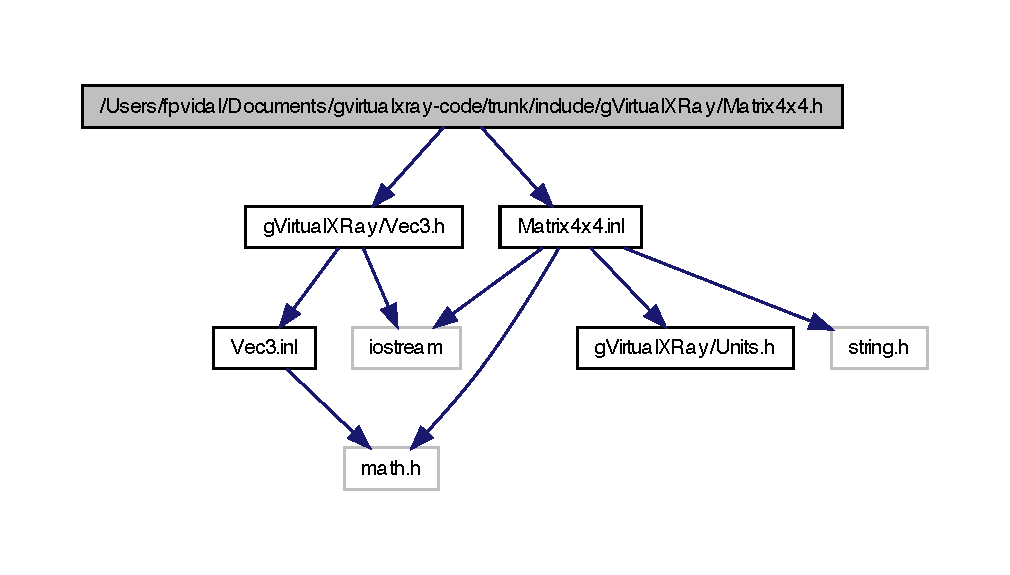
\includegraphics[width=400pt]{_matrix4x4_8h__incl}
\end{center}
\end{figure}
This graph shows which files directly or indirectly include this file:
\nopagebreak
\begin{figure}[H]
\begin{center}
\leavevmode
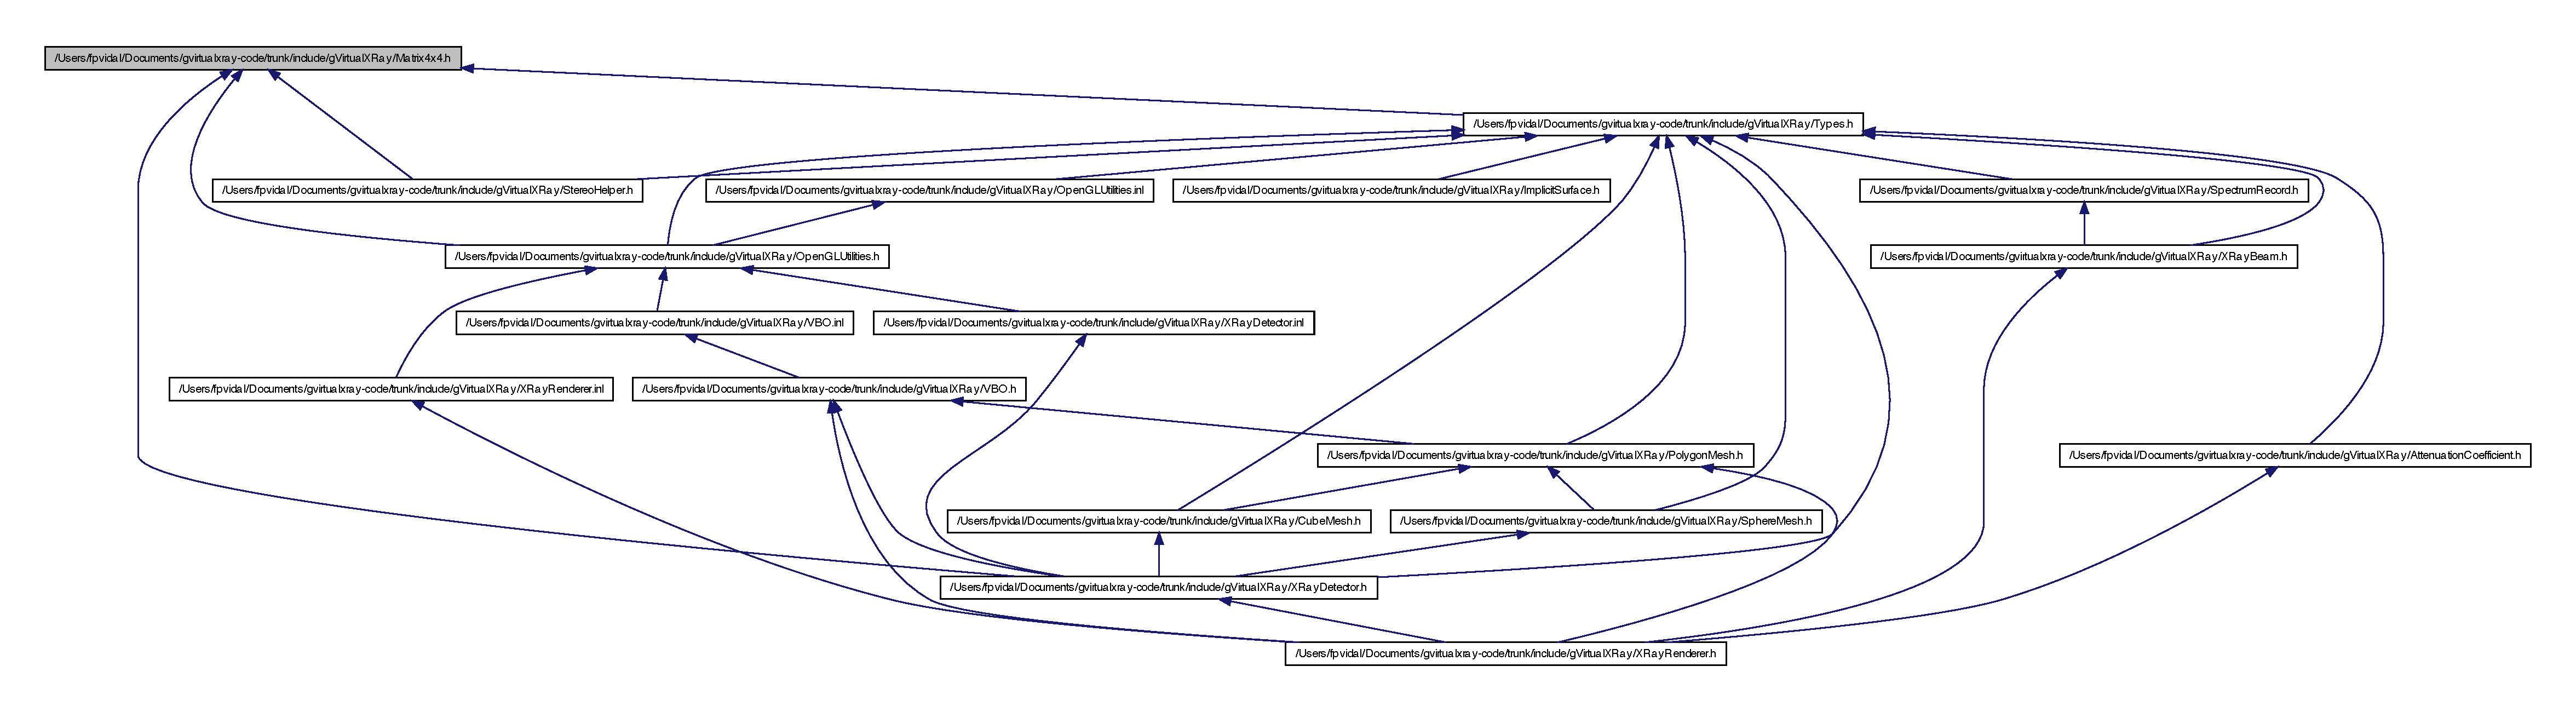
\includegraphics[width=400pt]{_matrix4x4_8h__dep__incl}
\end{center}
\end{figure}
\subsection*{Classes}
\begin{DoxyCompactItemize}
\item 
class \hyperlink{class_math_1_1_matrix4x4}{Math::Matrix4x4$<$ T $>$}
\begin{DoxyCompactList}\small\item\em \hyperlink{class_math_1_1_matrix4x4}{Matrix4x4} is a template class to handle a 4 by 4 matrix. \end{DoxyCompactList}\end{DoxyCompactItemize}
\subsection*{Namespaces}
\begin{DoxyCompactItemize}
\item 
namespace \hyperlink{namespace_math}{Math}
\end{DoxyCompactItemize}


\subsection{Detailed Description}
Template class to handle a 4x4 matrixs. \begin{DoxyVersion}{Version}
1.0
\end{DoxyVersion}
\begin{DoxyDate}{Date}
11/11/2013
\end{DoxyDate}
\begin{DoxyAuthor}{Author}
Dr Franck P. Vidal
\end{DoxyAuthor}
\hypertarget{_x_ray_renderer_8inl_License}{}\subsection{License}\label{_x_ray_renderer_8inl_License}
BSD 3-\/Clause License.

For details on use and redistribution please refer to \href{http://opensource.org/licenses/BSD-3-Clause}{\tt http://opensource.org/licenses/BSD-\/3-\/Clause}\hypertarget{_x_ray_renderer_8inl_Copyright}{}\subsection{Copyright}\label{_x_ray_renderer_8inl_Copyright}
(c) by Dr Franck P. Vidal (\href{mailto:franck.p.vidal@fpvidal.net}{\tt franck.p.vidal@fpvidal.net}), \href{http://www.fpvidal.net/,}{\tt http://www.fpvidal.net/,} Dec 2013, 2013, version 1.0, BSD 3-\/Clause License 

Definition in file \hyperlink{_matrix4x4_8h_source}{Matrix4x4.h}.


\hypertarget{_matrix4x4_8inl}{
\section{/Users/fpvidal/Documents/gvirtualxray-\/code/trunk/include/gVirtualXRay/Matrix4x4.inl File Reference}
\label{_matrix4x4_8inl}\index{/Users/fpvidal/Documents/gvirtualxray-\/code/trunk/include/gVirtualXRay/Matrix4x4.inl@{/Users/fpvidal/Documents/gvirtualxray-\/code/trunk/include/gVirtualXRay/Matrix4x4.inl}}
}


Template class to handle 4x4 matrices.  


{\ttfamily \#include \char`\"{}gVirtualXRay/Units.h\char`\"{}}\par
{\ttfamily \#include $<$iostream$>$}\par
{\ttfamily \#include $<$math.h$>$}\par
{\ttfamily \#include $<$string.h$>$}\par
Include dependency graph for Matrix4x4.inl:\nopagebreak
\begin{figure}[H]
\begin{center}
\leavevmode
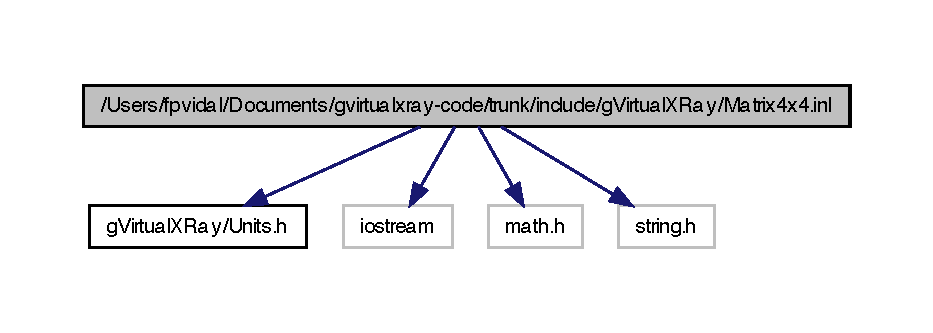
\includegraphics[width=400pt]{_matrix4x4_8inl__incl}
\end{center}
\end{figure}
This graph shows which files directly or indirectly include this file:
\nopagebreak
\begin{figure}[H]
\begin{center}
\leavevmode
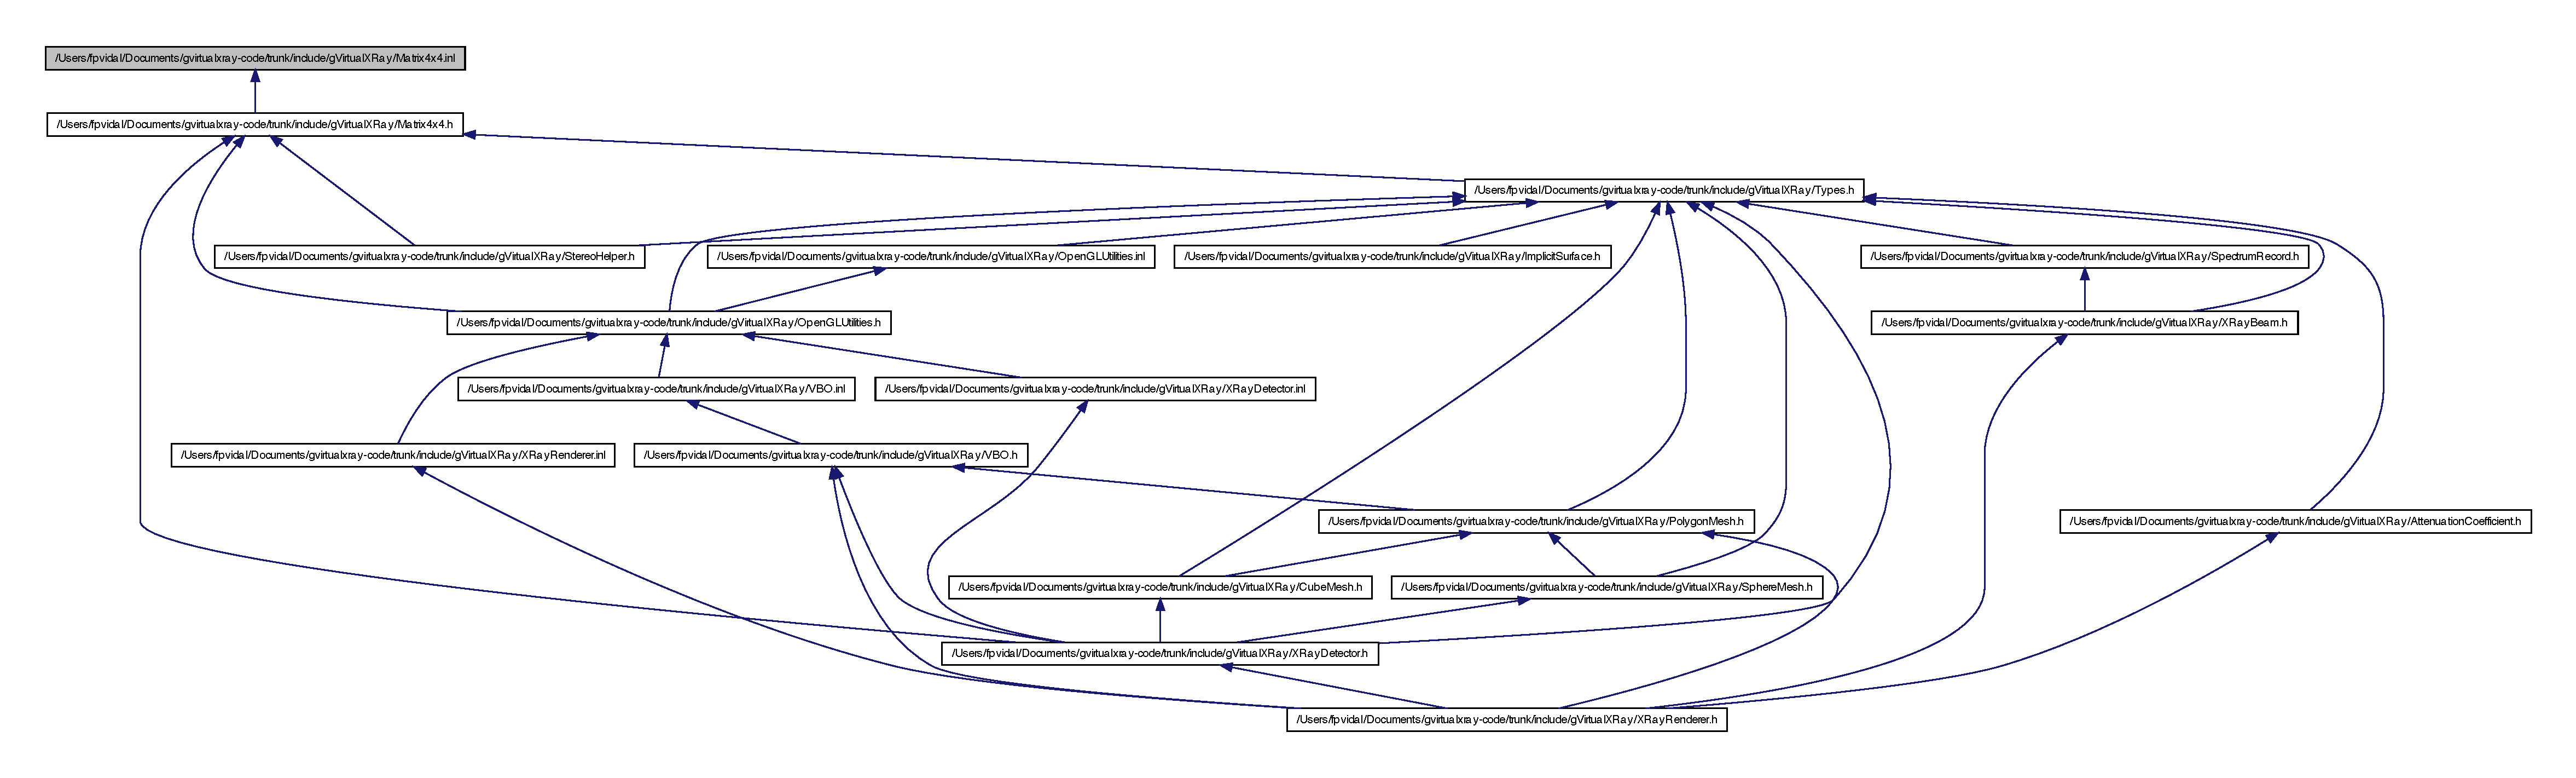
\includegraphics[width=400pt]{_matrix4x4_8inl__dep__incl}
\end{center}
\end{figure}
\subsection*{Namespaces}
\begin{DoxyCompactItemize}
\item 
namespace \hyperlink{namespace_math}{Math}
\end{DoxyCompactItemize}


\subsection{Detailed Description}
Template class to handle 4x4 matrices. \begin{DoxyVersion}{Version}
1.0
\end{DoxyVersion}
\begin{DoxyDate}{Date}
11/11/2013
\end{DoxyDate}
\begin{DoxyAuthor}{Author}
Dr Franck P. Vidal
\end{DoxyAuthor}
\hypertarget{_x_ray_renderer_8inl_License}{}\subsection{License}\label{_x_ray_renderer_8inl_License}
BSD 3-\/Clause License.

For details on use and redistribution please refer to \href{http://opensource.org/licenses/BSD-3-Clause}{\tt http://opensource.org/licenses/BSD-\/3-\/Clause}\hypertarget{_x_ray_renderer_8inl_Copyright}{}\subsection{Copyright}\label{_x_ray_renderer_8inl_Copyright}
(c) by Dr Franck P. Vidal (\href{mailto:franck.p.vidal@fpvidal.net}{\tt franck.p.vidal@fpvidal.net}), \href{http://www.fpvidal.net/,}{\tt http://www.fpvidal.net/,} Dec 2013, 2013, version 1.0, BSD 3-\/Clause License 

Definition in file \hyperlink{_matrix4x4_8inl_source}{Matrix4x4.inl}.


\hypertarget{_open_g_l_exception_8h}{
\section{/Users/fpvidal/Documents/gvirtualxray-\/code/trunk/include/gVirtualXRay/OpenGLException.h File Reference}
\label{_open_g_l_exception_8h}\index{/Users/fpvidal/Documents/gvirtualxray-\/code/trunk/include/gVirtualXRay/OpenGLException.h@{/Users/fpvidal/Documents/gvirtualxray-\/code/trunk/include/gVirtualXRay/OpenGLException.h}}
}


Class to handle exceptions related to frame buffer objects (FBOs).  


{\ttfamily \#include \char`\"{}gVirtualXRay/Exception.h\char`\"{}}\par
Include dependency graph for OpenGLException.h:\nopagebreak
\begin{figure}[H]
\begin{center}
\leavevmode
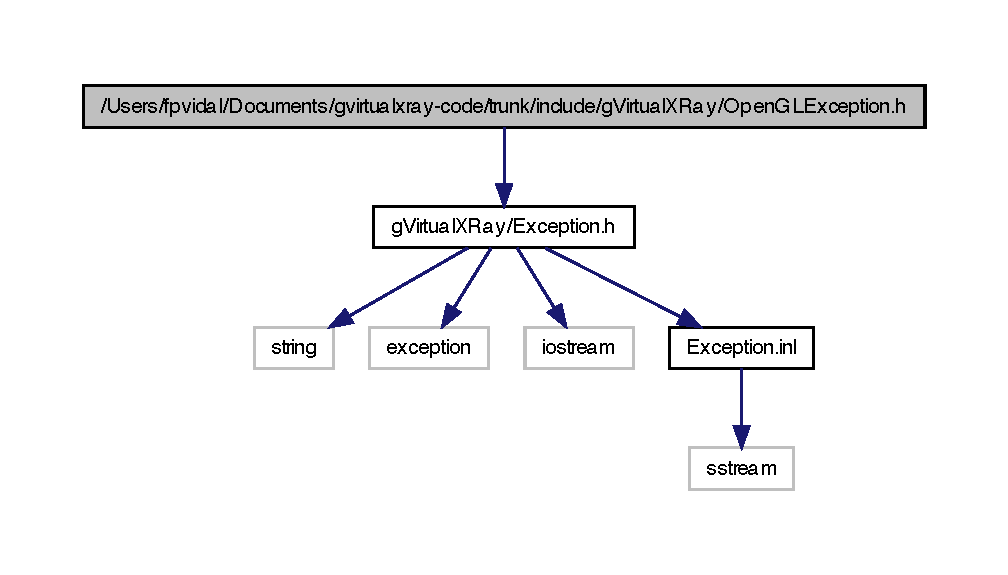
\includegraphics[width=400pt]{_open_g_l_exception_8h__incl}
\end{center}
\end{figure}
This graph shows which files directly or indirectly include this file:
\nopagebreak
\begin{figure}[H]
\begin{center}
\leavevmode
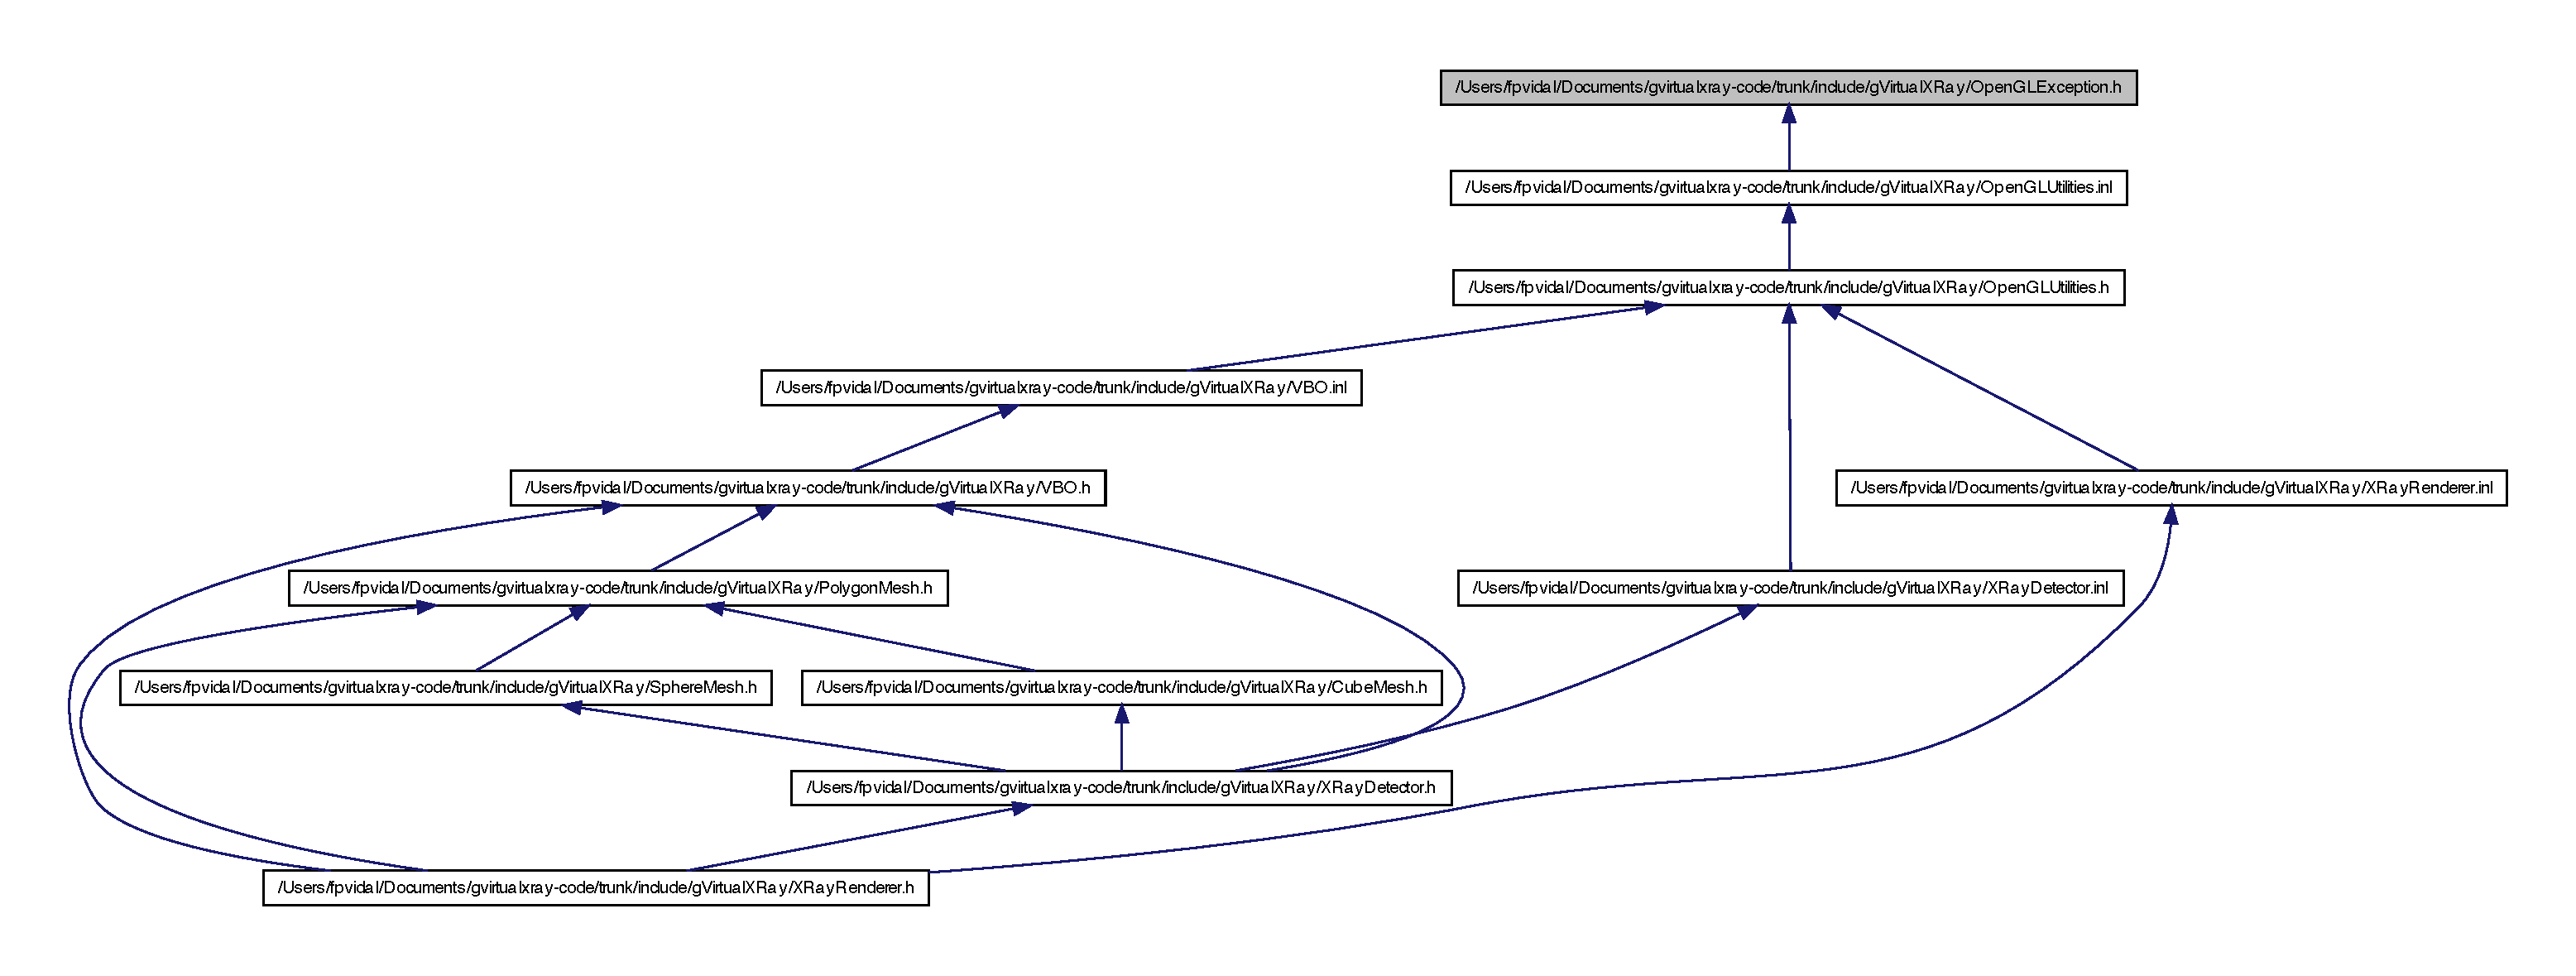
\includegraphics[width=400pt]{_open_g_l_exception_8h__dep__incl}
\end{center}
\end{figure}
\subsection*{Classes}
\begin{DoxyCompactItemize}
\item 
class \hyperlink{class_utilities_1_1_open_g_l_exception}{Utilities::OpenGLException}
\begin{DoxyCompactList}\small\item\em \hyperlink{class_utilities_1_1_open_g_l_exception}{OpenGLException} is a class to handle exceptions related to OpenGL. \end{DoxyCompactList}\end{DoxyCompactItemize}
\subsection*{Namespaces}
\begin{DoxyCompactItemize}
\item 
namespace \hyperlink{namespace_utilities}{Utilities}
\end{DoxyCompactItemize}


\subsection{Detailed Description}
Class to handle exceptions related to frame buffer objects (FBOs). Class to handle exceptions related to OpenGL.

\begin{DoxyVersion}{Version}
1.0
\end{DoxyVersion}
\begin{DoxyDate}{Date}
07/11/2013
\end{DoxyDate}
\begin{DoxyAuthor}{Author}
Dr Franck P. Vidal
\end{DoxyAuthor}
\hypertarget{_x_ray_renderer_8inl_License}{}\subsection{License}\label{_x_ray_renderer_8inl_License}
BSD 3-\/Clause License.

For details on use and redistribution please refer to \href{http://opensource.org/licenses/BSD-3-Clause}{\tt http://opensource.org/licenses/BSD-\/3-\/Clause}\hypertarget{_x_ray_renderer_8inl_Copyright}{}\subsection{Copyright}\label{_x_ray_renderer_8inl_Copyright}
(c) by Dr Franck P. Vidal (\href{mailto:franck.p.vidal@fpvidal.net}{\tt franck.p.vidal@fpvidal.net}), \href{http://www.fpvidal.net/,}{\tt http://www.fpvidal.net/,} Dec 2013, 2013, version 1.0, BSD 3-\/Clause License 

Definition in file \hyperlink{_open_g_l_exception_8h_source}{OpenGLException.h}.


\hypertarget{_open_g_l_utilities_8h}{
\section{/Users/fpvidal/Documents/gvirtualxray-\/code/trunk/include/gVirtualXRay/OpenGLUtilities.h File Reference}
\label{_open_g_l_utilities_8h}\index{/Users/fpvidal/Documents/gvirtualxray-\/code/trunk/include/gVirtualXRay/OpenGLUtilities.h@{/Users/fpvidal/Documents/gvirtualxray-\/code/trunk/include/gVirtualXRay/OpenGLUtilities.h}}
}


Some utility functions about OpenGL.  


{\ttfamily \#include $<$vector$>$}\par
{\ttfamily \#include \char`\"{}gVirtualXRay/Matrix4x4.h\char`\"{}}\par
{\ttfamily \#include \char`\"{}gVirtualXRay/Types.h\char`\"{}}\par
{\ttfamily \#include \char`\"{}OpenGLUtilities.inl\char`\"{}}\par
Include dependency graph for OpenGLUtilities.h:\nopagebreak
\begin{figure}[H]
\begin{center}
\leavevmode
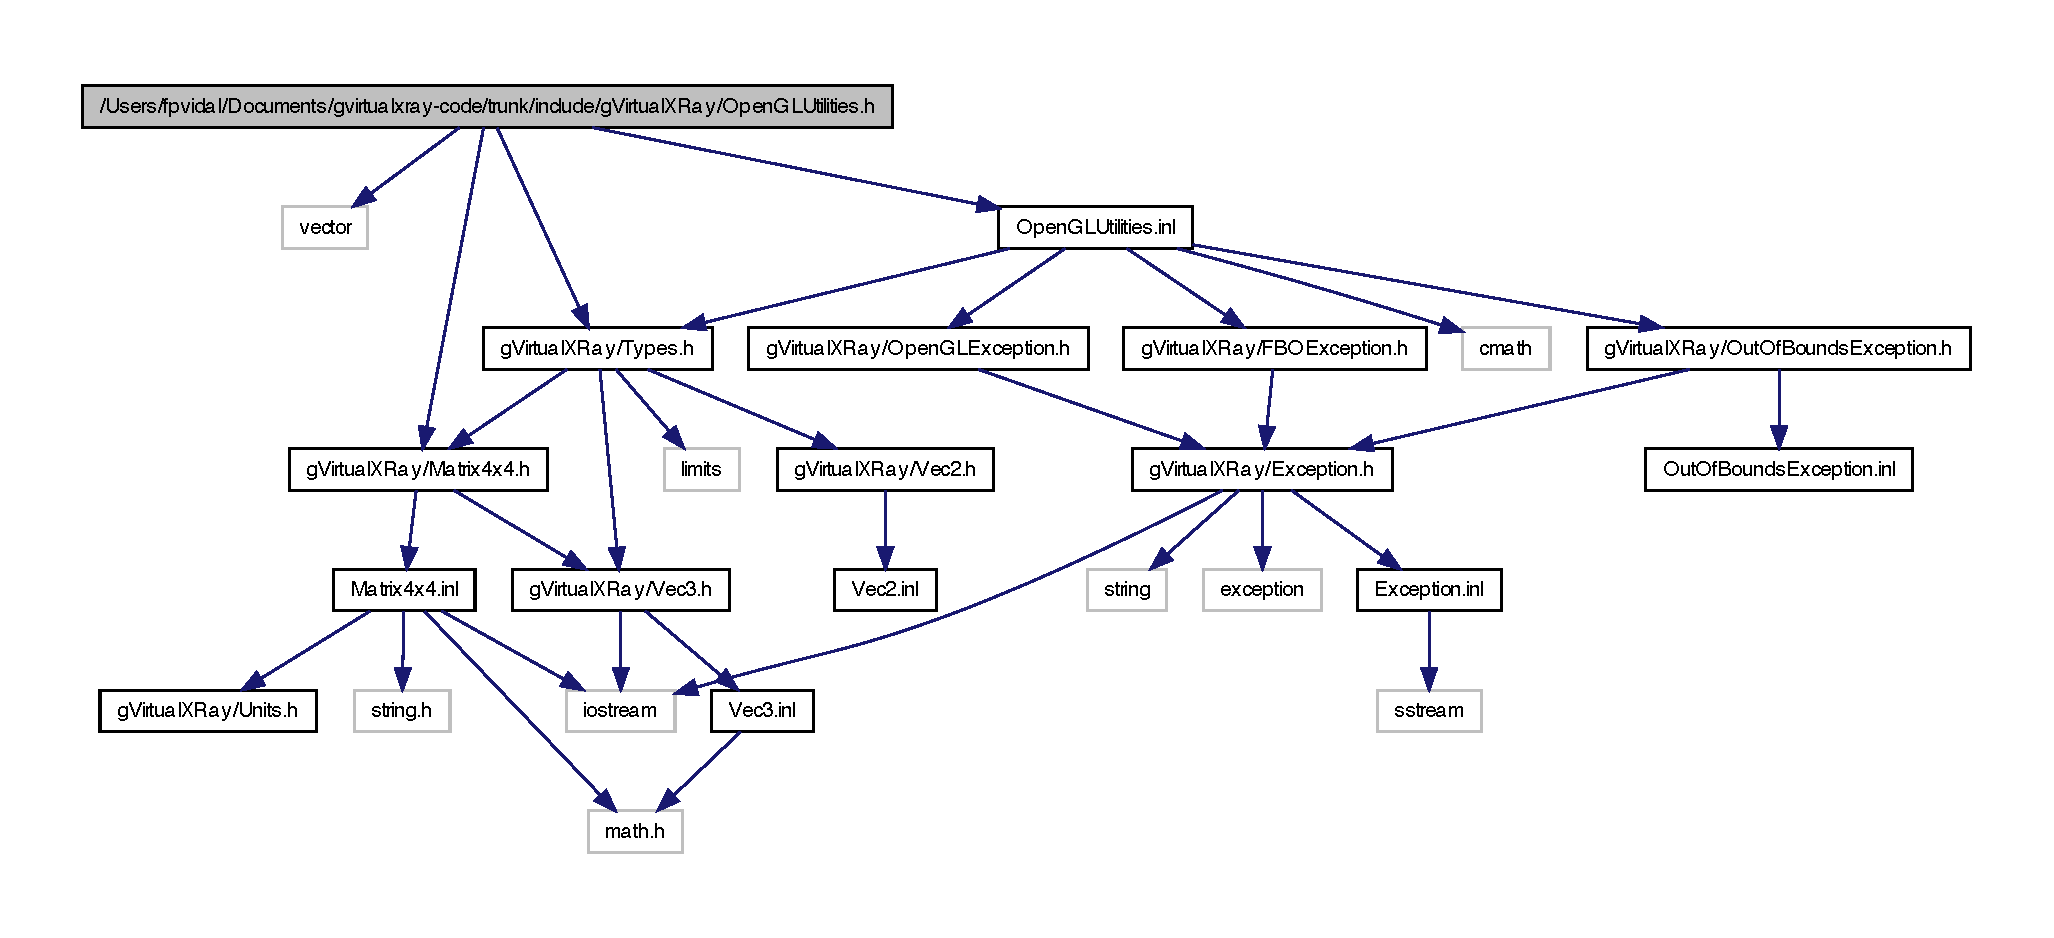
\includegraphics[width=400pt]{_open_g_l_utilities_8h__incl}
\end{center}
\end{figure}
This graph shows which files directly or indirectly include this file:
\nopagebreak
\begin{figure}[H]
\begin{center}
\leavevmode
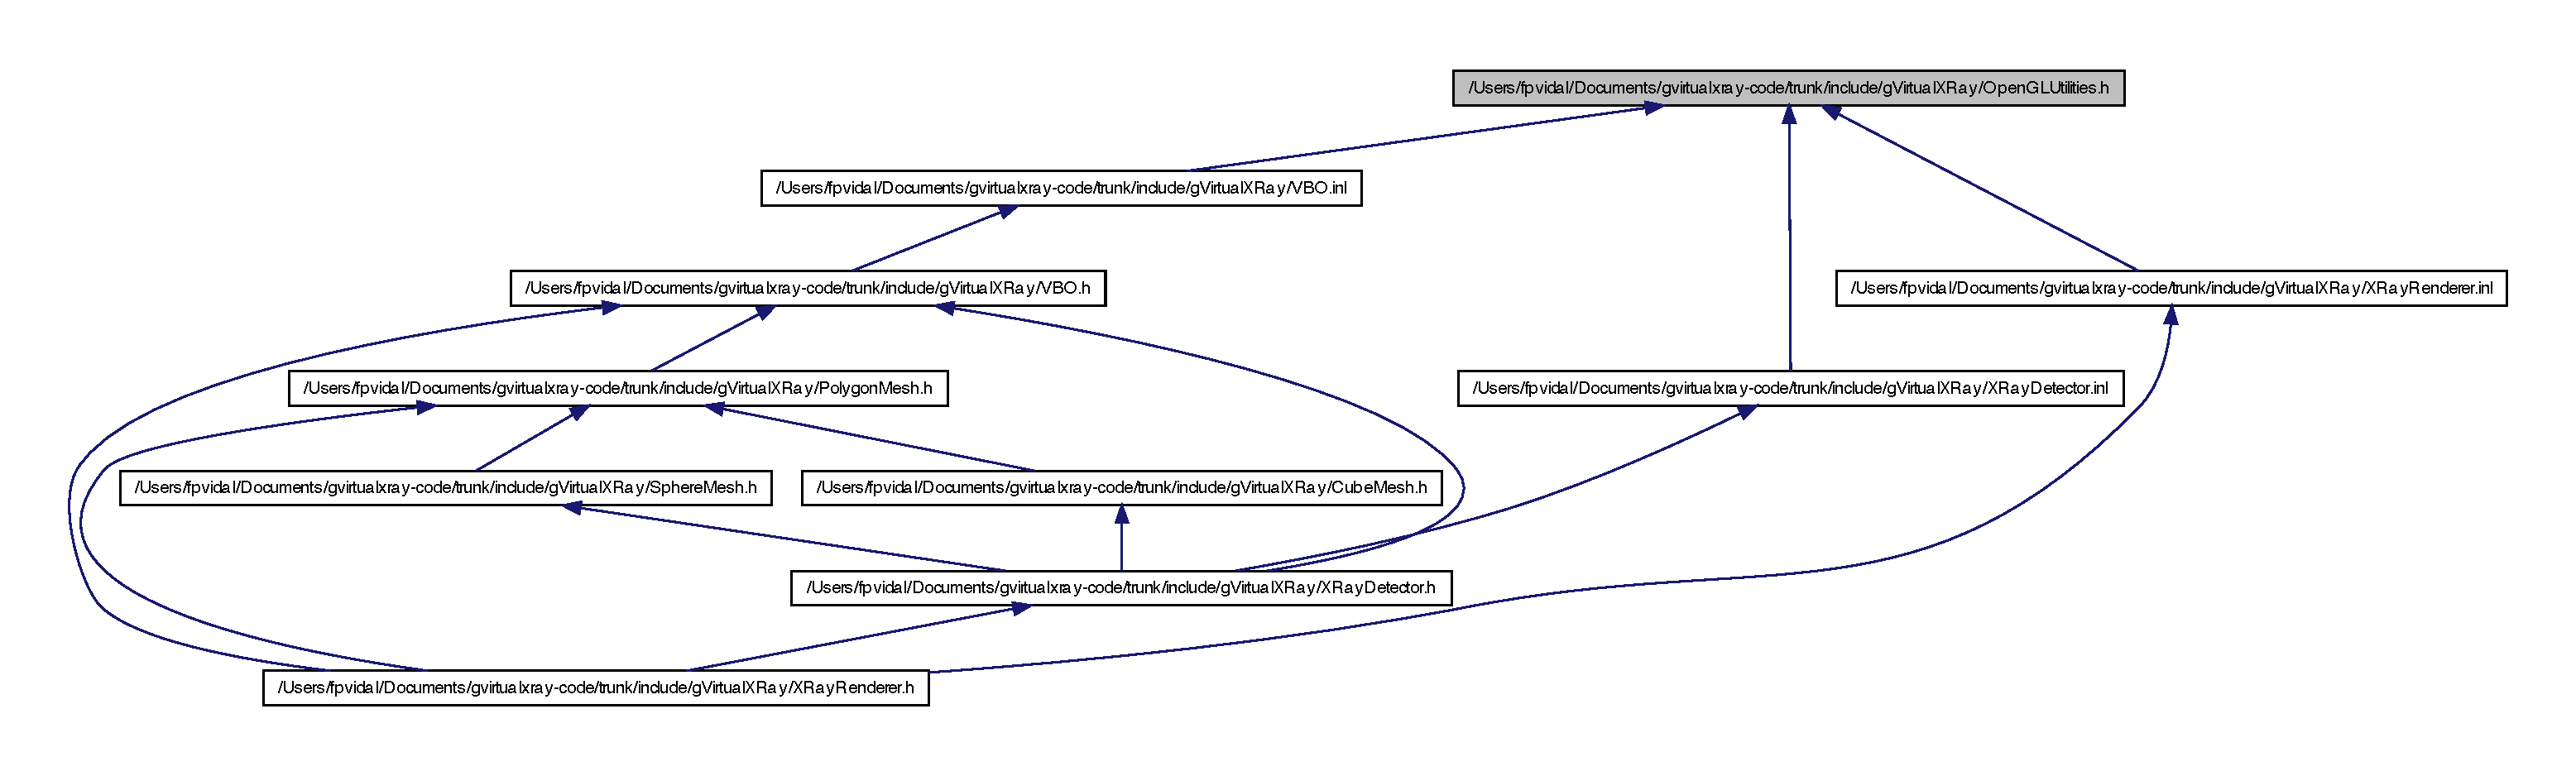
\includegraphics[width=400pt]{_open_g_l_utilities_8h__dep__incl}
\end{center}
\end{figure}
\subsection*{Namespaces}
\begin{DoxyCompactItemize}
\item 
namespace \hyperlink{namespace_utilities}{Utilities}
\end{DoxyCompactItemize}
\subsection*{Functions}
\begin{DoxyCompactItemize}
\item 
void \hyperlink{namespace_utilities_ac80bf2d2d0e6f362b9fa305c6329d4dd}{Utilities::checkOpenGLErrorStatus} (const char $\ast$aFileName, const char $\ast$aFunctionName, int aLineNumber)
\begin{DoxyCompactList}\small\item\em Check OpenGL's error status. \end{DoxyCompactList}\item 
void \hyperlink{namespace_utilities_aa6d370633a054fc0d3867e172c410b8f}{Utilities::checkFBOErrorStatus} (const char $\ast$aFileName, const char $\ast$aFunctionName, int aLineNumber)
\begin{DoxyCompactList}\small\item\em Check the current FBO's error status. \end{DoxyCompactList}\item 
void \hyperlink{namespace_utilities_a4ff1a91f49f45940ef3fe39374d6fad3}{Utilities::pushProjectionMatrix} ()
\begin{DoxyCompactList}\small\item\em Add the current matrix to the projection matrix stack. \end{DoxyCompactList}\item 
void \hyperlink{namespace_utilities_a759523b332a302b032d7e1dbe3d70589}{Utilities::pushModelViewMatrix} ()
\begin{DoxyCompactList}\small\item\em Add the current matrix to the model/view matrix stack. \end{DoxyCompactList}\item 
void \hyperlink{namespace_utilities_a4d73d1a6deada0aace5a5fb250971aa1}{Utilities::pushFBO} ()
\begin{DoxyCompactList}\small\item\em Add the current FBO binding to the FBO stack. \end{DoxyCompactList}\item 
void \hyperlink{namespace_utilities_acc7a477a449c637b37acf6e409ffda9a}{Utilities::pushTexture1D} ()
\begin{DoxyCompactList}\small\item\em Add the current 1D texture binding to the texture stack. \end{DoxyCompactList}\item 
void \hyperlink{namespace_utilities_ac3f7c9af73fc18c8e905ec33e423e62a}{Utilities::pushTexture2D} ()
\begin{DoxyCompactList}\small\item\em Add the current 2D texture binding to the texture stack. \end{DoxyCompactList}\item 
void \hyperlink{namespace_utilities_ade797d2da463a1e1774e46fb1519a3a6}{Utilities::pushTextureRectangle} ()
\begin{DoxyCompactList}\small\item\em Add the current rectangle texture binding to the texture stack. \end{DoxyCompactList}\item 
void \hyperlink{namespace_utilities_a6c5b0b068baed228d72a5ab5bc171a27}{Utilities::pushTexture3D} ()
\begin{DoxyCompactList}\small\item\em Add the current 3D texture binding to the texture stack. \end{DoxyCompactList}\item 
void \hyperlink{namespace_utilities_a397b32b08d50b0f86540e20ec9d9a8a6}{Utilities::pushEnableDisableState} (int aParameter)
\begin{DoxyCompactList}\small\item\em Add the enable/disable state to the corresponding stack. \end{DoxyCompactList}\item 
void \hyperlink{namespace_utilities_af3def433e5459d13617b1f3ac1f80bd4}{Utilities::pushShaderProgram} ()
\begin{DoxyCompactList}\small\item\em Add the current shader program to the corresponding stack. \end{DoxyCompactList}\item 
void \hyperlink{namespace_utilities_a34e5aecb15bd70f3d358b1df30ad2b1e}{Utilities::popProjectionMatrix} ()
\item 
void \hyperlink{namespace_utilities_afa855d36de0ce9d6d52e2157da5063b9}{Utilities::popModelViewMatrix} ()
\item 
void \hyperlink{namespace_utilities_a155eb0147d0e117e1d34467ce4bf8495}{Utilities::popFBO} ()
\item 
void \hyperlink{namespace_utilities_a399fdac28547b4cab45f640befd6350a}{Utilities::popTexture} ()
\item 
void \hyperlink{namespace_utilities_a74d082f280da485386fb80a2a65cf36a}{Utilities::popEnableDisableState} ()
\item 
void \hyperlink{namespace_utilities_adbc5643c5d6336e174b6bea3a22bdb29}{Utilities::popShaderProgram} ()
\item 
\hyperlink{class_math_1_1_matrix4x4}{Math::Matrix4x4}$<$ float $>$ \hyperlink{namespace_utilities_a27ecbb568ab30c335d210de98b739757}{Utilities::getCurrentOpenGLMatrix} ()
\begin{DoxyCompactList}\small\item\em Load the current OpenGL matrix. \end{DoxyCompactList}\item 
void \hyperlink{namespace_utilities_af4402f472bd1945b6792f547cd498f95}{Utilities::loadIdentityProjectionMatrix} ()
\begin{DoxyCompactList}\small\item\em Replace the projection matrix by the identity matrix. \end{DoxyCompactList}\item 
void \hyperlink{namespace_utilities_a80dad624c31abf68e2e44997020210a5}{Utilities::loadIdentityModelViewMatrix} ()
\begin{DoxyCompactList}\small\item\em Replace the model/view matrix by the identity matrix. \end{DoxyCompactList}\item 
void \hyperlink{namespace_utilities_ad6cddf27e1b4769a998710f48a74026d}{Utilities::loadFrustumProjectionMatrix} (double left, double right, double bottom, double top, double near, double far)
\begin{DoxyCompactList}\small\item\em Replace the projection matrix by a perspective projection matrix. \end{DoxyCompactList}\item 
void \hyperlink{namespace_utilities_a72a4f2b2d67dc75de5b6ebbf25248521}{Utilities::loadPerspectiveProjectionMatrix} (double fovy, double aspect, double zNear, double zFar)
\begin{DoxyCompactList}\small\item\em Replace the projection matrix by a perspective projection matrix. \end{DoxyCompactList}\item 
void \hyperlink{namespace_utilities_ae239a07fe9373e6a079a8c1465cab662}{Utilities::loadOrthoProjectionMatrix} (double left, double right, double bottom, double top, double near, double far)
\begin{DoxyCompactList}\small\item\em Replace the projection matrix by a orthographic projection matrix. \end{DoxyCompactList}\item 
MATRIX4 \hyperlink{namespace_utilities_a7ffbee866eb154b2a032141c04d43021}{Utilities::buildOrthoProjectionMatrix} (double left, double right, double bottom, double top, double near, double far)
\begin{DoxyCompactList}\small\item\em Create a orthographic projection matrix. \end{DoxyCompactList}\item 
MATRIX4 \hyperlink{namespace_utilities_aaa85ac0797b49093c4344ce75c4a3265}{Utilities::buildFrustumProjectionMatrix} (double left, double right, double bottom, double top, double near, double far)
\begin{DoxyCompactList}\small\item\em Create a perspective projection matrix. \end{DoxyCompactList}\item 
MATRIX4 \hyperlink{namespace_utilities_ae473d6bd8d417fc07465944092a92938}{Utilities::buildPerspectiveProjectionMatrix} (double fovy, double aspect, double zNear, double zFar)
\begin{DoxyCompactList}\small\item\em Create a perspective projection matrix. \end{DoxyCompactList}\item 
void \hyperlink{namespace_utilities_adcb191e43b838d267bd659167503a528}{Utilities::loadLookAtModelViewMatrix} (const VEC3 \&eye, const VEC3 \&centre, const VEC3 \&up)
\begin{DoxyCompactList}\small\item\em Replace the modelling-\/viewing matrix by a viewing transformation matrix. \end{DoxyCompactList}\item 
void \hyperlink{namespace_utilities_a8dfe8f9df9a5280d2b19e278b6c455eb}{Utilities::loadLookAtModelViewMatrix} (double eyeX, double eyeY, double eyeZ, double centreX, double centreY, double centreZ, double upX, double upY, double upZ)
\begin{DoxyCompactList}\small\item\em Replace the modelling-\/viewing matrix by a viewing transformation matrix. \end{DoxyCompactList}\item 
MATRIX4 \hyperlink{namespace_utilities_a84ad75173a3da5e4e8b355d03d100c59}{Utilities::buildLookAtModelViewMatrix} (const VEC3 \&eye, const VEC3 \&centre, const VEC3 \&up)
\begin{DoxyCompactList}\small\item\em Create a modelling-\/viewing matrix. \end{DoxyCompactList}\item 
MATRIX4 \hyperlink{namespace_utilities_a0dfa7bb57b5c491451a43d8b4d7dd983}{Utilities::buildLookAtModelViewMatrix} (double eyeX, double eyeY, double eyeZ, double centreX, double centreY, double centreZ, double upX, double upY, double upZ)
\begin{DoxyCompactList}\small\item\em Create a modelling-\/viewing matrix. \end{DoxyCompactList}\item 
void \hyperlink{namespace_utilities_a1787b9d17f79b46cd3fc546bfd9ee196}{Utilities::loadProjectionMatrixFromOpenGL} ()
\begin{DoxyCompactList}\small\item\em Replace the projection matrix by OpenGL's projection matrix. \end{DoxyCompactList}\item 
void \hyperlink{namespace_utilities_a8cc5454fb226411756900e06f3b121b2}{Utilities::loadModelViewMatrixFromOpenGL} ()
\begin{DoxyCompactList}\small\item\em Replace the modelling-\/viewing matrix by OpenGL's modelling-\/viewing matrix. \end{DoxyCompactList}\item 
void \hyperlink{namespace_utilities_a3fdfd69b196f894ae78f35a055d8683e}{Utilities::applyModelViewMatrix} ()
\end{DoxyCompactItemize}
\subsection*{Variables}
\begin{DoxyCompactItemize}
\item 
std::vector$<$ MATRIX4 $>$ \hyperlink{namespace_utilities_af9f46e572978db79176b61edb1780b3c}{Utilities::g\_\-p\_\-modelview\_\-matrix\_\-stack}
\begin{DoxyCompactList}\small\item\em The stack of model/view matrices. \end{DoxyCompactList}\item 
std::vector$<$ MATRIX4 $>$ \hyperlink{namespace_utilities_a3e2a3a6c251bba50ffe4c069d085e0b7}{Utilities::g\_\-p\_\-projection\_\-matrix\_\-stack}
\begin{DoxyCompactList}\small\item\em The stack of projection matrix. \end{DoxyCompactList}\item 
MATRIX4 \hyperlink{namespace_utilities_accdb6ed1387ebfbb3458b12fc5104fc0}{Utilities::g\_\-current\_\-modelview\_\-matrix}
\begin{DoxyCompactList}\small\item\em The model/view matrices. \end{DoxyCompactList}\item 
MATRIX4 \hyperlink{namespace_utilities_a8c2454e701dfbb5ec835d7d3a36869c5}{Utilities::g\_\-current\_\-projection\_\-matrix}
\begin{DoxyCompactList}\small\item\em The projection matrix. \end{DoxyCompactList}\item 
std::vector$<$ int $>$ \hyperlink{namespace_utilities_a0c685e4387f8e43c77ef5931a213cfaf}{Utilities::g\_\-frame\_\-buffer\_\-object\_\-stack}
\begin{DoxyCompactList}\small\item\em The stack of FBO binding. \end{DoxyCompactList}\item 
std::vector$<$ std::pair$<$ int, int $>$ $>$ \hyperlink{namespace_utilities_a0f11bcfd46f3b7d0bdf66bc2127ba85f}{Utilities::g\_\-texture\_\-stack}
\begin{DoxyCompactList}\small\item\em The stack of texture binding. \end{DoxyCompactList}\item 
std::vector$<$ std::pair$<$ int, bool $>$ $>$ \hyperlink{namespace_utilities_a12dfa64d0c2f8186e94336a73defa7a8}{Utilities::g\_\-enable\_\-disable\_\-state\_\-stack}
\begin{DoxyCompactList}\small\item\em The stack of enable/disable states. \end{DoxyCompactList}\item 
std::vector$<$ int $>$ \hyperlink{namespace_utilities_adf21242b77777527da1f9e6d8f72a1e5}{Utilities::g\_\-shader\_\-program\_\-stack}
\begin{DoxyCompactList}\small\item\em The stack of shader programs. \end{DoxyCompactList}\end{DoxyCompactItemize}


\subsection{Detailed Description}
Some utility functions about OpenGL. \begin{DoxyVersion}{Version}
1.0
\end{DoxyVersion}
\begin{DoxyDate}{Date}
07/11/2013
\end{DoxyDate}
\begin{DoxyAuthor}{Author}
Dr Franck P. Vidal
\end{DoxyAuthor}
\hypertarget{_x_ray_renderer_8inl_License}{}\subsection{License}\label{_x_ray_renderer_8inl_License}
BSD 3-\/Clause License.

For details on use and redistribution please refer to \href{http://opensource.org/licenses/BSD-3-Clause}{\tt http://opensource.org/licenses/BSD-\/3-\/Clause}\hypertarget{_x_ray_renderer_8inl_Copyright}{}\subsection{Copyright}\label{_x_ray_renderer_8inl_Copyright}
(c) by Dr Franck P. Vidal (\href{mailto:franck.p.vidal@fpvidal.net}{\tt franck.p.vidal@fpvidal.net}), \href{http://www.fpvidal.net/,}{\tt http://www.fpvidal.net/,} Dec 2013, 2013, version 1.0, BSD 3-\/Clause License 

Definition in file \hyperlink{_open_g_l_utilities_8h_source}{OpenGLUtilities.h}.


\hypertarget{_open_g_l_utilities_8inl}{
\section{/Users/fpvidal/Documents/gvirtualxray-\/code/trunk/include/gVirtualXRay/OpenGLUtilities.inl File Reference}
\label{_open_g_l_utilities_8inl}\index{/Users/fpvidal/Documents/gvirtualxray-\/code/trunk/include/gVirtualXRay/OpenGLUtilities.inl@{/Users/fpvidal/Documents/gvirtualxray-\/code/trunk/include/gVirtualXRay/OpenGLUtilities.inl}}
}


Some utility functions about OpenGL.  


{\ttfamily \#include $<$cmath$>$}\par
{\ttfamily \#include \char`\"{}gVirtualXRay/OpenGLException.h\char`\"{}}\par
{\ttfamily \#include \char`\"{}gVirtualXRay/OutOfBoundsException.h\char`\"{}}\par
{\ttfamily \#include \char`\"{}gVirtualXRay/FBOException.h\char`\"{}}\par
{\ttfamily \#include \char`\"{}gVirtualXRay/Types.h\char`\"{}}\par
Include dependency graph for OpenGLUtilities.inl:\nopagebreak
\begin{figure}[H]
\begin{center}
\leavevmode
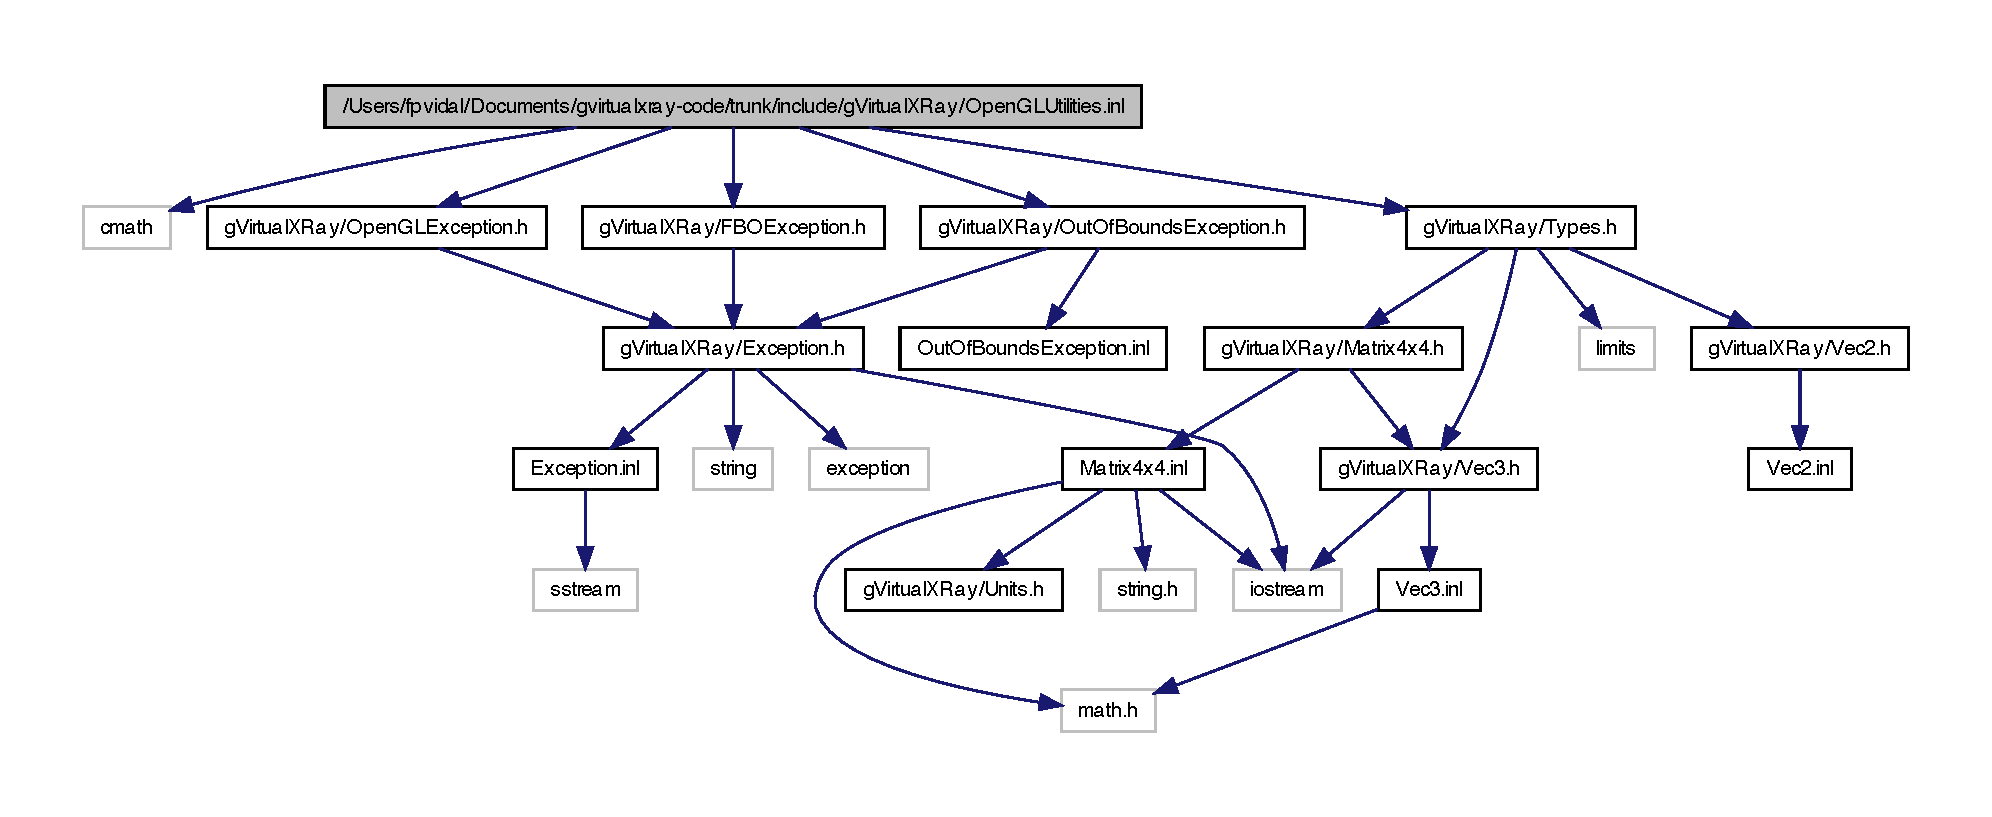
\includegraphics[width=400pt]{_open_g_l_utilities_8inl__incl}
\end{center}
\end{figure}
This graph shows which files directly or indirectly include this file:
\nopagebreak
\begin{figure}[H]
\begin{center}
\leavevmode
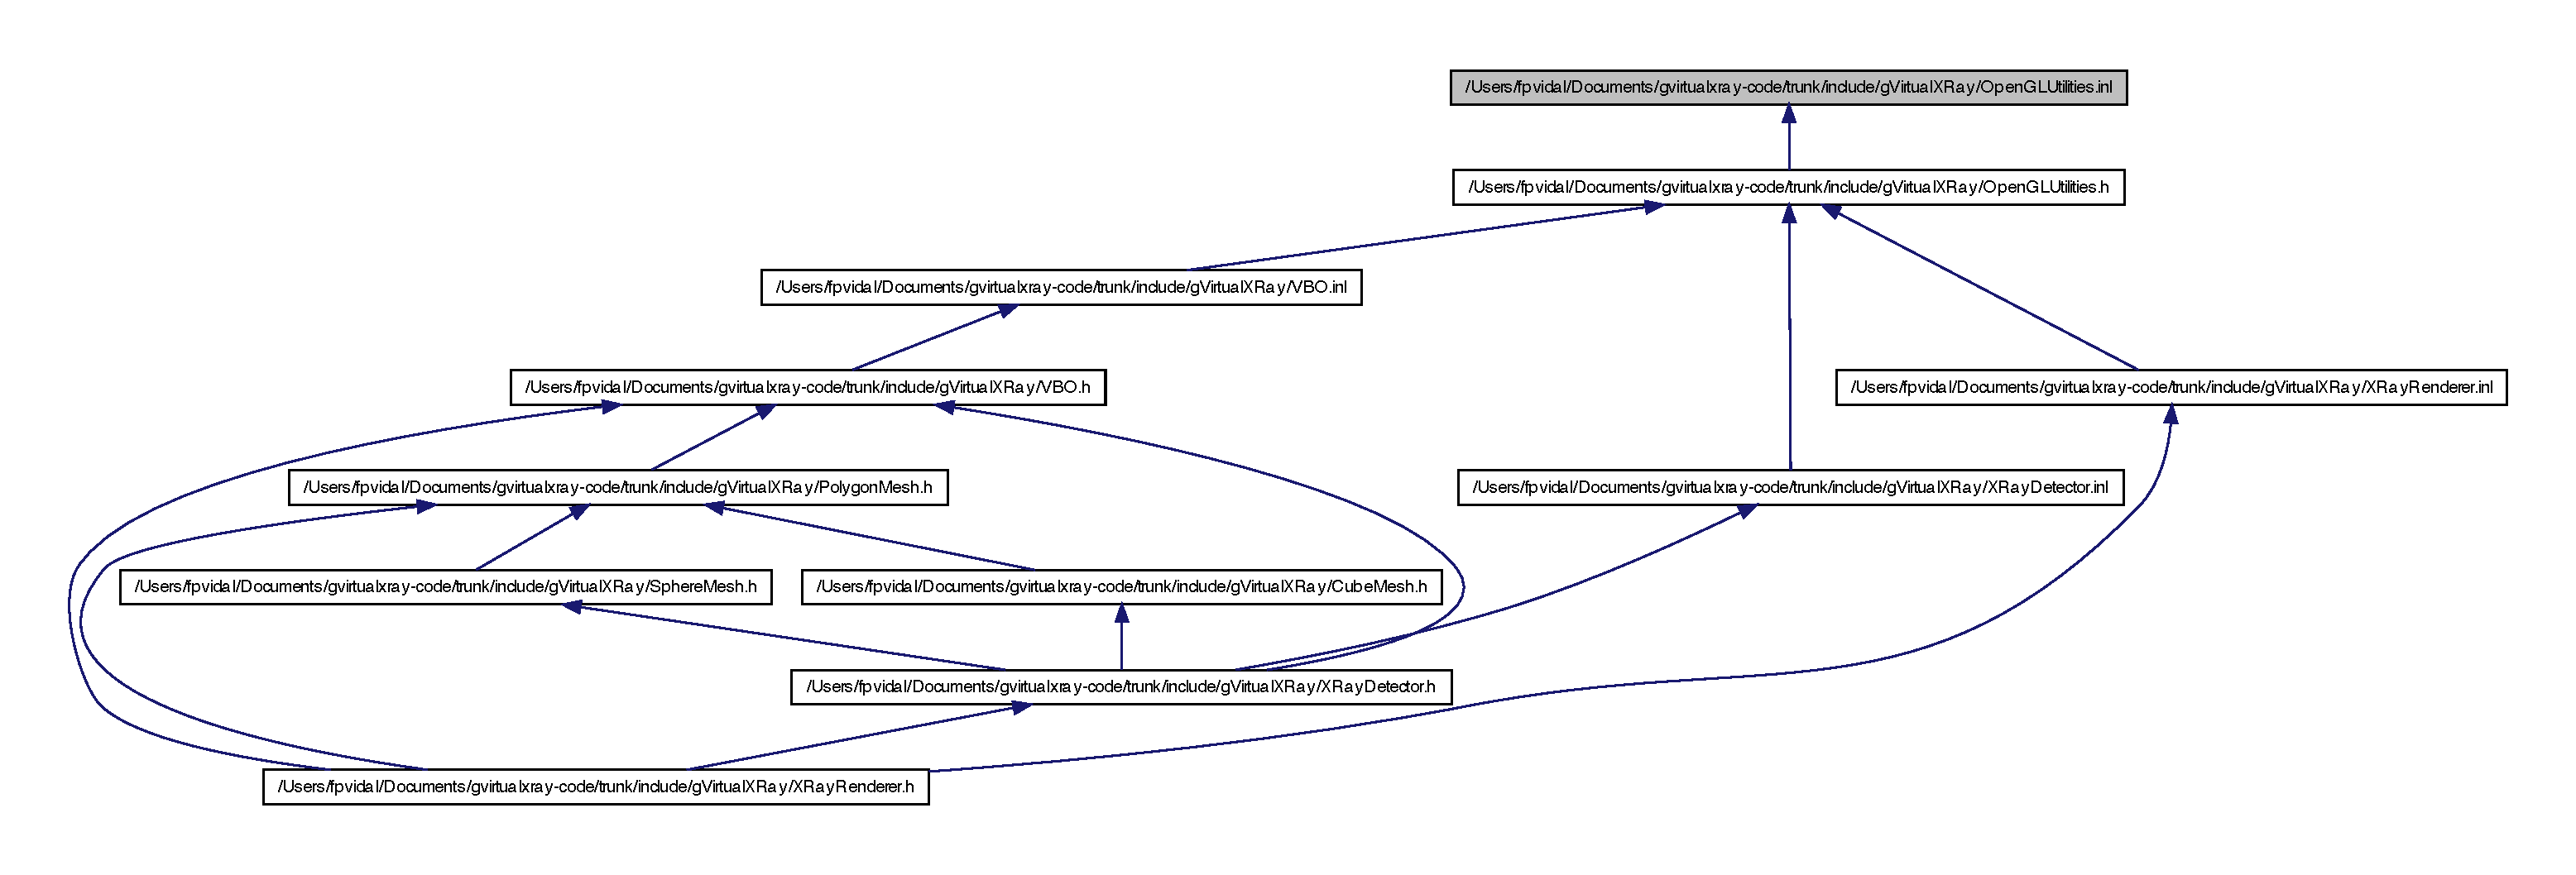
\includegraphics[width=400pt]{_open_g_l_utilities_8inl__dep__incl}
\end{center}
\end{figure}
\subsection*{Namespaces}
\begin{DoxyCompactItemize}
\item 
namespace \hyperlink{namespace_utilities}{Utilities}
\end{DoxyCompactItemize}
\subsection*{Functions}
\begin{DoxyCompactItemize}
\item 
void \hyperlink{namespace_utilities_a4ff1a91f49f45940ef3fe39374d6fad3}{Utilities::pushProjectionMatrix} ()
\begin{DoxyCompactList}\small\item\em Add the current matrix to the projection matrix stack. \end{DoxyCompactList}\item 
void \hyperlink{namespace_utilities_a759523b332a302b032d7e1dbe3d70589}{Utilities::pushModelViewMatrix} ()
\begin{DoxyCompactList}\small\item\em Add the current matrix to the model/view matrix stack. \end{DoxyCompactList}\item 
void \hyperlink{namespace_utilities_a34e5aecb15bd70f3d358b1df30ad2b1e}{Utilities::popProjectionMatrix} ()
\item 
void \hyperlink{namespace_utilities_afa855d36de0ce9d6d52e2157da5063b9}{Utilities::popModelViewMatrix} ()
\item 
void \hyperlink{namespace_utilities_af4402f472bd1945b6792f547cd498f95}{Utilities::loadIdentityProjectionMatrix} ()
\begin{DoxyCompactList}\small\item\em Replace the projection matrix by the identity matrix. \end{DoxyCompactList}\item 
void \hyperlink{namespace_utilities_a80dad624c31abf68e2e44997020210a5}{Utilities::loadIdentityModelViewMatrix} ()
\begin{DoxyCompactList}\small\item\em Replace the model/view matrix by the identity matrix. \end{DoxyCompactList}\item 
MATRIX4 \hyperlink{namespace_utilities_a7ffbee866eb154b2a032141c04d43021}{Utilities::buildOrthoProjectionMatrix} (double left, double right, double bottom, double top, double near, double far)
\begin{DoxyCompactList}\small\item\em Create a orthographic projection matrix. \end{DoxyCompactList}\item 
void \hyperlink{namespace_utilities_ae239a07fe9373e6a079a8c1465cab662}{Utilities::loadOrthoProjectionMatrix} (double left, double right, double bottom, double top, double near, double far)
\begin{DoxyCompactList}\small\item\em Replace the projection matrix by a orthographic projection matrix. \end{DoxyCompactList}\item 
void \hyperlink{namespace_utilities_ad6cddf27e1b4769a998710f48a74026d}{Utilities::loadFrustumProjectionMatrix} (double left, double right, double bottom, double top, double near, double far)
\begin{DoxyCompactList}\small\item\em Replace the projection matrix by a perspective projection matrix. \end{DoxyCompactList}\item 
MATRIX4 \hyperlink{namespace_utilities_aaa85ac0797b49093c4344ce75c4a3265}{Utilities::buildFrustumProjectionMatrix} (double left, double right, double bottom, double top, double near, double far)
\begin{DoxyCompactList}\small\item\em Create a perspective projection matrix. \end{DoxyCompactList}\item 
void \hyperlink{namespace_utilities_ab6a11c99ddae551a4d7bc64d18d63046}{Utilities::multiplyOrthoProjectionMatrix} (double left, double right, double bottom, double top, double nearPlane, double farPlane)
\item 
MATRIX4 \hyperlink{namespace_utilities_ae473d6bd8d417fc07465944092a92938}{Utilities::buildPerspectiveProjectionMatrix} (double fovy, double aspect, double zNear, double zFar)
\begin{DoxyCompactList}\small\item\em Create a perspective projection matrix. \end{DoxyCompactList}\item 
void \hyperlink{namespace_utilities_a72a4f2b2d67dc75de5b6ebbf25248521}{Utilities::loadPerspectiveProjectionMatrix} (double fovy, double aspect, double zNear, double zFar)
\begin{DoxyCompactList}\small\item\em Replace the projection matrix by a perspective projection matrix. \end{DoxyCompactList}\item 
void \hyperlink{namespace_utilities_aaf402e609cb9931c8534ac08968fb49b}{Utilities::multiplyPerspectiveProjectionMatrix} (double fovy, double aspect, double zNear, double zFar)
\item 
MATRIX4 \hyperlink{namespace_utilities_a84ad75173a3da5e4e8b355d03d100c59}{Utilities::buildLookAtModelViewMatrix} (const VEC3 \&eye, const VEC3 \&centre, const VEC3 \&up)
\begin{DoxyCompactList}\small\item\em Create a modelling-\/viewing matrix. \end{DoxyCompactList}\item 
MATRIX4 \hyperlink{namespace_utilities_a0dfa7bb57b5c491451a43d8b4d7dd983}{Utilities::buildLookAtModelViewMatrix} (double eyeX, double eyeY, double eyeZ, double centreX, double centreY, double centreZ, double upX, double upY, double upZ)
\begin{DoxyCompactList}\small\item\em Create a modelling-\/viewing matrix. \end{DoxyCompactList}\item 
void \hyperlink{namespace_utilities_adcb191e43b838d267bd659167503a528}{Utilities::loadLookAtModelViewMatrix} (const VEC3 \&eye, const VEC3 \&centre, const VEC3 \&up)
\begin{DoxyCompactList}\small\item\em Replace the modelling-\/viewing matrix by a viewing transformation matrix. \end{DoxyCompactList}\item 
void \hyperlink{namespace_utilities_a8dfe8f9df9a5280d2b19e278b6c455eb}{Utilities::loadLookAtModelViewMatrix} (double eyeX, double eyeY, double eyeZ, double centreX, double centreY, double centreZ, double upX, double upY, double upZ)
\begin{DoxyCompactList}\small\item\em Replace the modelling-\/viewing matrix by a viewing transformation matrix. \end{DoxyCompactList}\end{DoxyCompactItemize}


\subsection{Detailed Description}
Some utility functions about OpenGL. \begin{DoxyVersion}{Version}
1.0
\end{DoxyVersion}
\begin{DoxyDate}{Date}
07/11/2013
\end{DoxyDate}
\begin{DoxyAuthor}{Author}
Dr Franck P. Vidal
\end{DoxyAuthor}
\hypertarget{_x_ray_renderer_8inl_License}{}\subsection{License}\label{_x_ray_renderer_8inl_License}
BSD 3-\/Clause License.

For details on use and redistribution please refer to \href{http://opensource.org/licenses/BSD-3-Clause}{\tt http://opensource.org/licenses/BSD-\/3-\/Clause}\hypertarget{_x_ray_renderer_8inl_Copyright}{}\subsection{Copyright}\label{_x_ray_renderer_8inl_Copyright}
(c) by Dr Franck P. Vidal (\href{mailto:franck.p.vidal@fpvidal.net}{\tt franck.p.vidal@fpvidal.net}), \href{http://www.fpvidal.net/,}{\tt http://www.fpvidal.net/,} Dec 2013, 2013, version 1.0, BSD 3-\/Clause License 

Definition in file \hyperlink{_open_g_l_utilities_8inl_source}{OpenGLUtilities.inl}.


\hypertarget{_out_of_bounds_exception_8h}{
\section{/Users/fpvidal/Documents/gvirtualxray-\/code/trunk/include/gVirtualXRay/OutOfBoundsException.h File Reference}
\label{_out_of_bounds_exception_8h}\index{/Users/fpvidal/Documents/gvirtualxray-\/code/trunk/include/gVirtualXRay/OutOfBoundsException.h@{/Users/fpvidal/Documents/gvirtualxray-\/code/trunk/include/gVirtualXRay/OutOfBoundsException.h}}
}


Class to handle exceptions when accessing an array cell that is not accessible, i.e. out of bounds memory access.  


{\ttfamily \#include \char`\"{}gVirtualXRay/Exception.h\char`\"{}}\par
{\ttfamily \#include \char`\"{}OutOfBoundsException.inl\char`\"{}}\par
Include dependency graph for OutOfBoundsException.h:\nopagebreak
\begin{figure}[H]
\begin{center}
\leavevmode
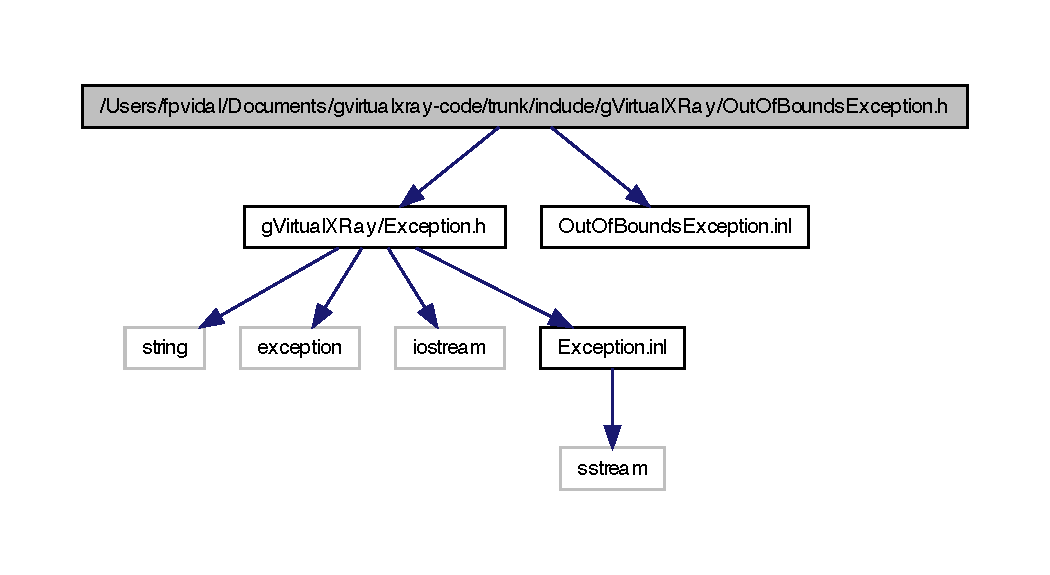
\includegraphics[width=400pt]{_out_of_bounds_exception_8h__incl}
\end{center}
\end{figure}
This graph shows which files directly or indirectly include this file:
\nopagebreak
\begin{figure}[H]
\begin{center}
\leavevmode
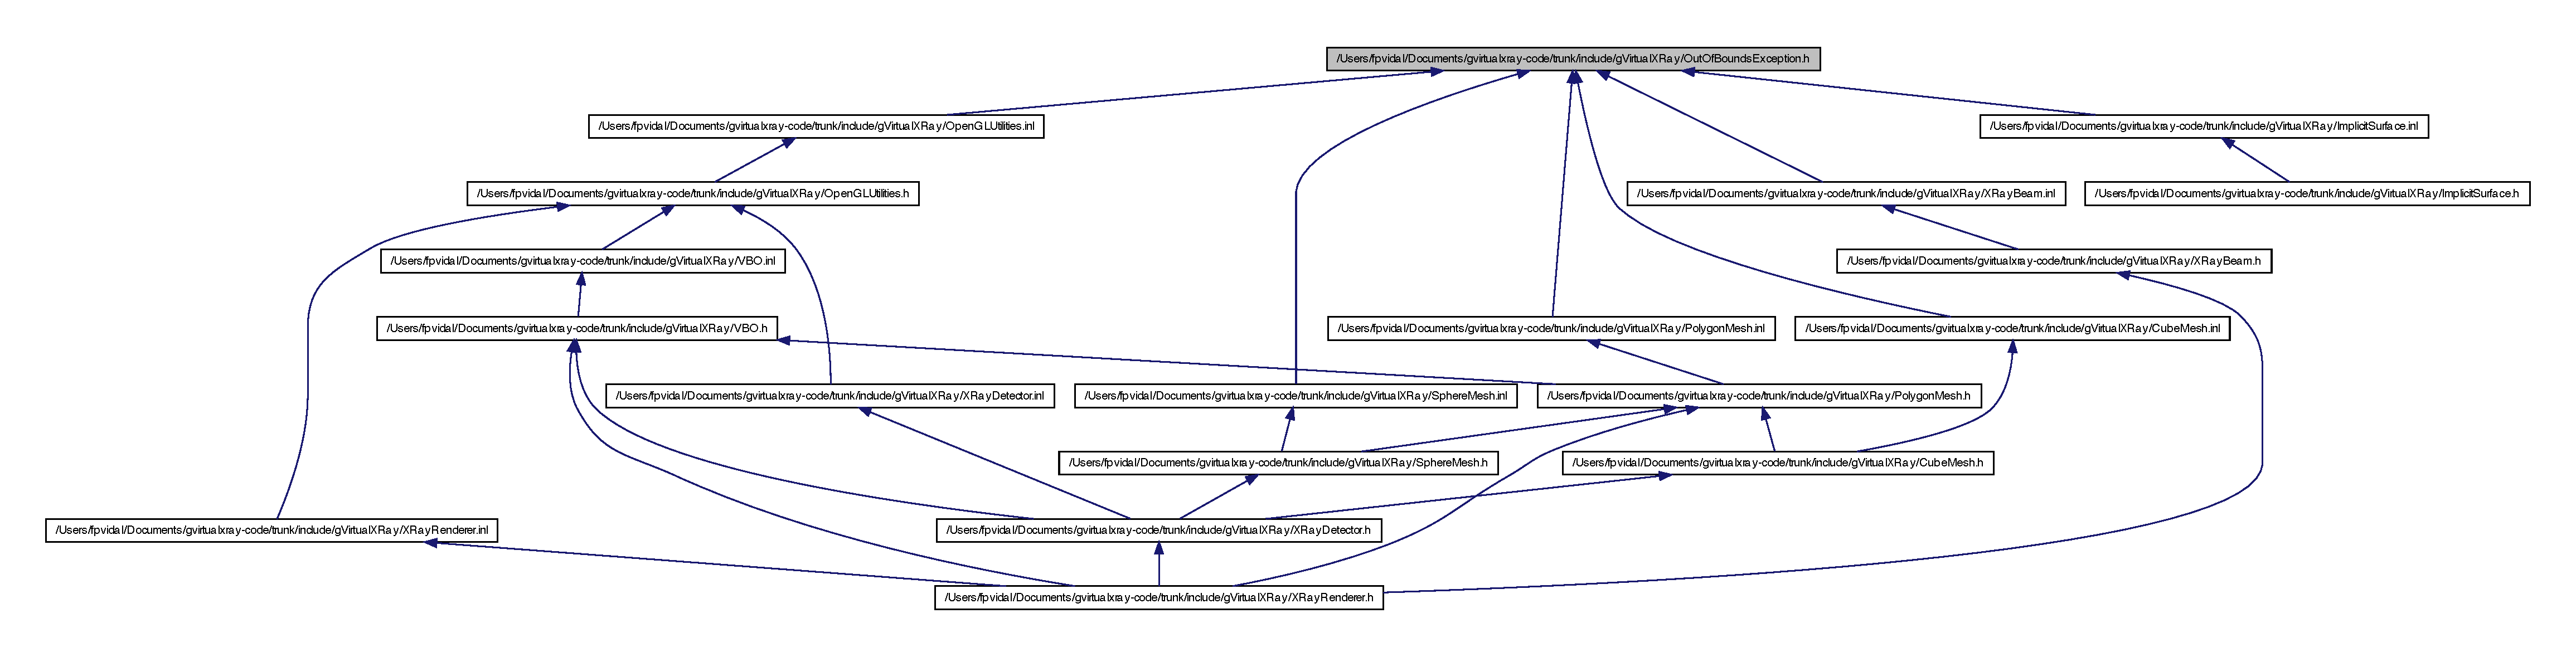
\includegraphics[width=400pt]{_out_of_bounds_exception_8h__dep__incl}
\end{center}
\end{figure}
\subsection*{Classes}
\begin{DoxyCompactItemize}
\item 
class \hyperlink{class_utilities_1_1_out_of_bounds_exception}{Utilities::OutOfBoundsException}
\end{DoxyCompactItemize}
\subsection*{Namespaces}
\begin{DoxyCompactItemize}
\item 
namespace \hyperlink{namespace_utilities}{Utilities}
\end{DoxyCompactItemize}


\subsection{Detailed Description}
Class to handle exceptions when accessing an array cell that is not accessible, i.e. out of bounds memory access. \begin{DoxyVersion}{Version}
1.0
\end{DoxyVersion}
\begin{DoxyDate}{Date}
30/11/2013
\end{DoxyDate}
\begin{DoxyAuthor}{Author}
Dr Franck P. Vidal
\end{DoxyAuthor}
\hypertarget{_x_ray_renderer_8inl_License}{}\subsection{License}\label{_x_ray_renderer_8inl_License}
BSD 3-\/Clause License.

For details on use and redistribution please refer to \href{http://opensource.org/licenses/BSD-3-Clause}{\tt http://opensource.org/licenses/BSD-\/3-\/Clause}\hypertarget{_x_ray_renderer_8inl_Copyright}{}\subsection{Copyright}\label{_x_ray_renderer_8inl_Copyright}
(c) by Dr Franck P. Vidal (\href{mailto:franck.p.vidal@fpvidal.net}{\tt franck.p.vidal@fpvidal.net}), \href{http://www.fpvidal.net/,}{\tt http://www.fpvidal.net/,} Dec 2013, 2013, version 1.0, BSD 3-\/Clause License 

Definition in file \hyperlink{_out_of_bounds_exception_8h_source}{OutOfBoundsException.h}.


\hypertarget{_out_of_bounds_exception_8inl}{
\section{/Users/fpvidal/Documents/gvirtualxray-\/code/trunk/include/gVirtualXRay/OutOfBoundsException.inl File Reference}
\label{_out_of_bounds_exception_8inl}\index{/Users/fpvidal/Documents/gvirtualxray-\/code/trunk/include/gVirtualXRay/OutOfBoundsException.inl@{/Users/fpvidal/Documents/gvirtualxray-\/code/trunk/include/gVirtualXRay/OutOfBoundsException.inl}}
}


Class to handle exceptions when accessing an array cell that is not accessible, i.e. out of bounds memory access.  


This graph shows which files directly or indirectly include this file:
\nopagebreak
\begin{figure}[H]
\begin{center}
\leavevmode
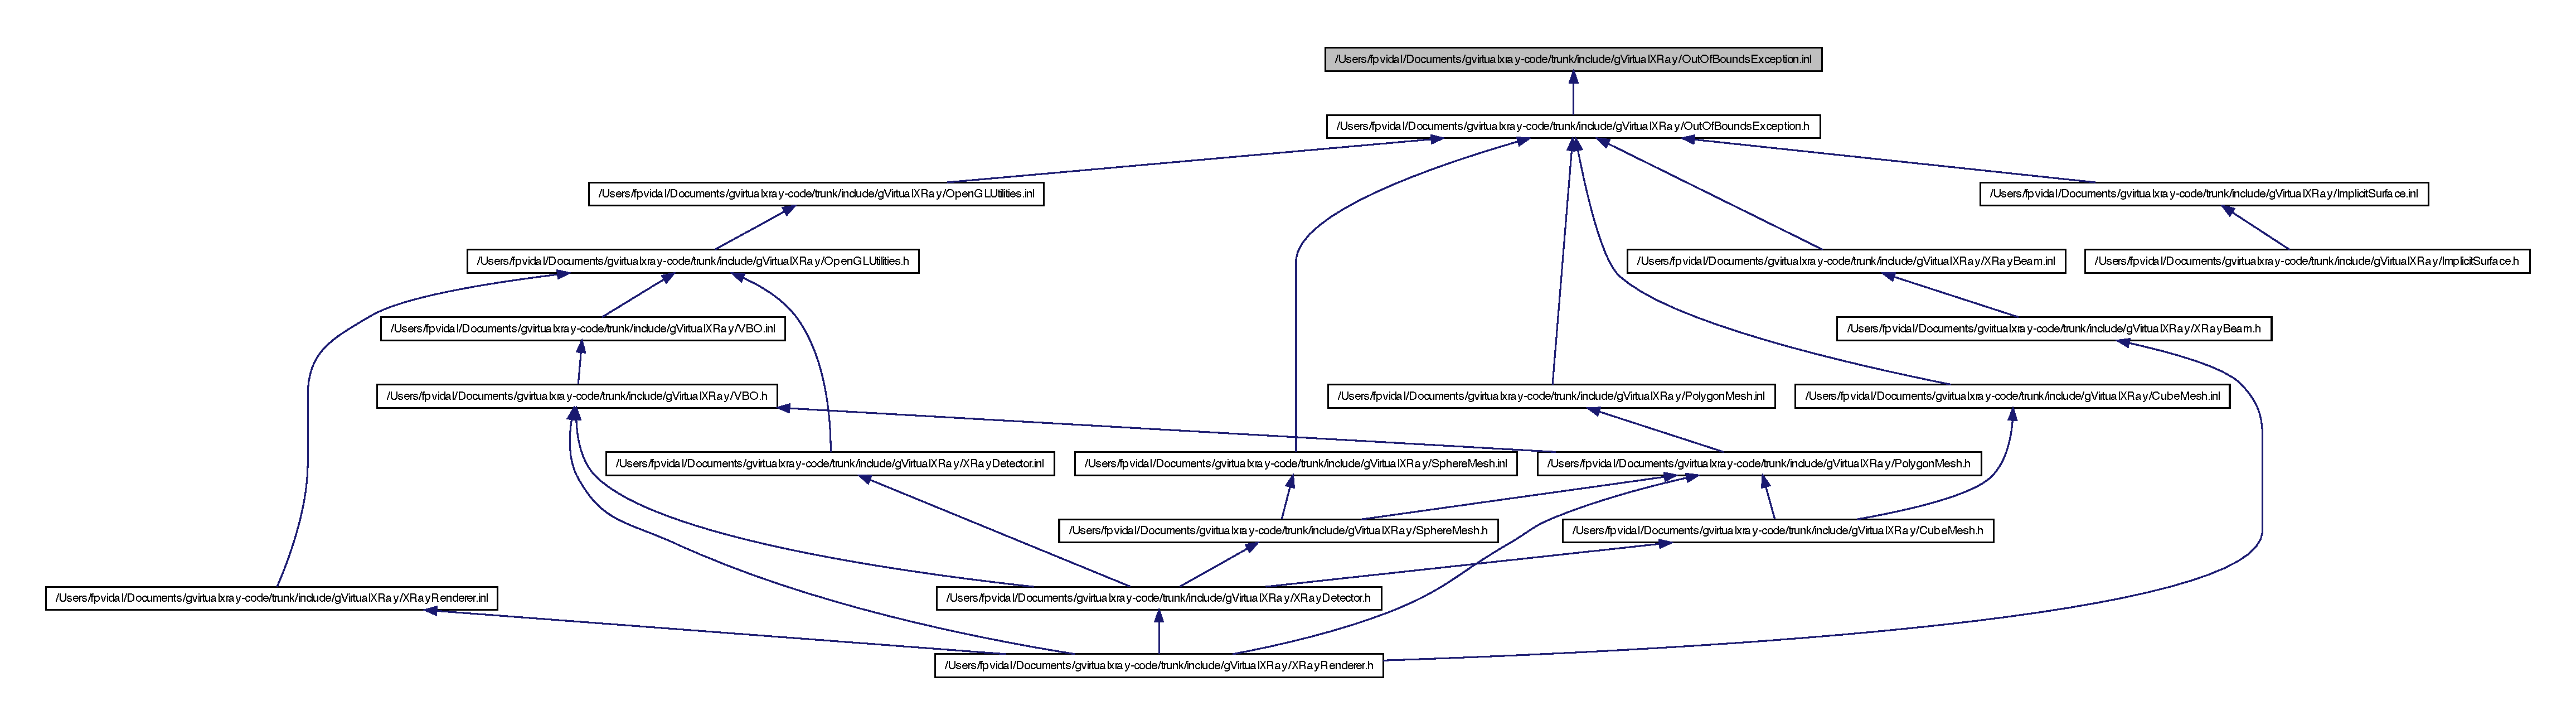
\includegraphics[width=400pt]{_out_of_bounds_exception_8inl__dep__incl}
\end{center}
\end{figure}
\subsection*{Namespaces}
\begin{DoxyCompactItemize}
\item 
namespace \hyperlink{namespace_utilities}{Utilities}
\end{DoxyCompactItemize}


\subsection{Detailed Description}
Class to handle exceptions when accessing an array cell that is not accessible, i.e. out of bounds memory access. \begin{DoxyVersion}{Version}
1.0
\end{DoxyVersion}
\begin{DoxyDate}{Date}
30/11/2013
\end{DoxyDate}
\begin{DoxyAuthor}{Author}
Dr Franck P. Vidal
\end{DoxyAuthor}
\hypertarget{_x_ray_renderer_8inl_License}{}\subsection{License}\label{_x_ray_renderer_8inl_License}
BSD 3-\/Clause License.

For details on use and redistribution please refer to \href{http://opensource.org/licenses/BSD-3-Clause}{\tt http://opensource.org/licenses/BSD-\/3-\/Clause}\hypertarget{_x_ray_renderer_8inl_Copyright}{}\subsection{Copyright}\label{_x_ray_renderer_8inl_Copyright}
(c) by Dr Franck P. Vidal (\href{mailto:franck.p.vidal@fpvidal.net}{\tt franck.p.vidal@fpvidal.net}), \href{http://www.fpvidal.net/,}{\tt http://www.fpvidal.net/,} Dec 2013, 2013, version 1.0, BSD 3-\/Clause License 

Definition in file \hyperlink{_out_of_bounds_exception_8inl_source}{OutOfBoundsException.inl}.


\hypertarget{_out_of_memory_exception_8h}{
\section{/Users/fpvidal/Documents/gvirtualxray-\/code/trunk/include/gVirtualXRay/OutOfMemoryException.h File Reference}
\label{_out_of_memory_exception_8h}\index{/Users/fpvidal/Documents/gvirtualxray-\/code/trunk/include/gVirtualXRay/OutOfMemoryException.h@{/Users/fpvidal/Documents/gvirtualxray-\/code/trunk/include/gVirtualXRay/OutOfMemoryException.h}}
}


Class to handle exceptions when memory cannot be allocated dynamically.  


{\ttfamily \#include \char`\"{}gVirtualXRay/Exception.h\char`\"{}}\par
{\ttfamily \#include \char`\"{}OutOfMemoryException.inl\char`\"{}}\par
Include dependency graph for OutOfMemoryException.h:\nopagebreak
\begin{figure}[H]
\begin{center}
\leavevmode
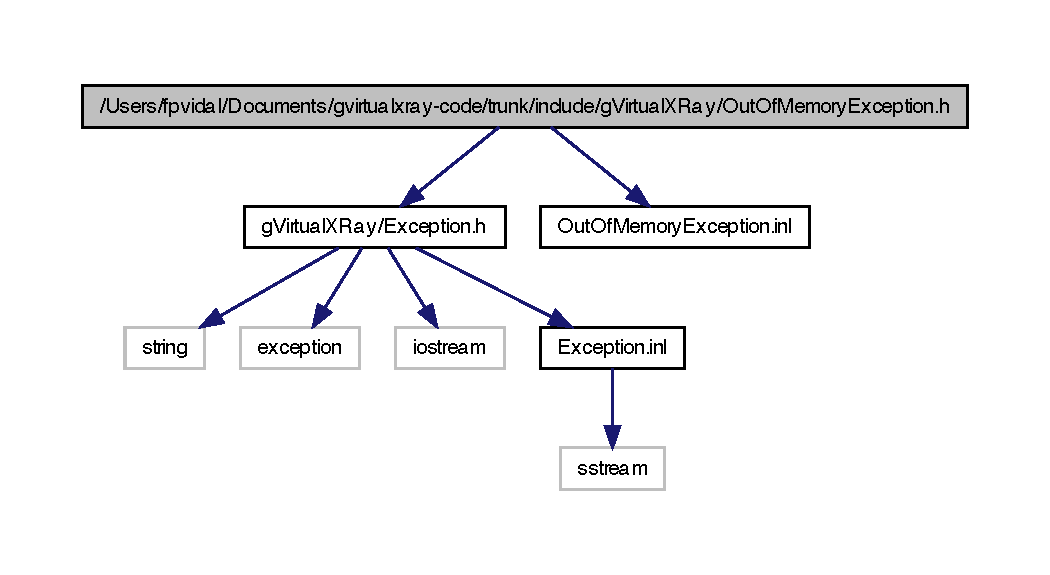
\includegraphics[width=400pt]{_out_of_memory_exception_8h__incl}
\end{center}
\end{figure}
\subsection*{Classes}
\begin{DoxyCompactItemize}
\item 
class \hyperlink{class_utilities_1_1_out_of_memory_exception}{Utilities::OutOfMemoryException}
\begin{DoxyCompactList}\small\item\em \hyperlink{class_utilities_1_1_out_of_memory_exception}{OutOfMemoryException} is a class to handle exceptions when accessing an array cell that is not accessible, i.e. out of bounds memory access. \end{DoxyCompactList}\end{DoxyCompactItemize}
\subsection*{Namespaces}
\begin{DoxyCompactItemize}
\item 
namespace \hyperlink{namespace_utilities}{Utilities}
\end{DoxyCompactItemize}


\subsection{Detailed Description}
Class to handle exceptions when memory cannot be allocated dynamically. \begin{DoxyVersion}{Version}
1.0
\end{DoxyVersion}
\begin{DoxyDate}{Date}
30/11/2013
\end{DoxyDate}
\begin{DoxyAuthor}{Author}
Dr Franck P. Vidal
\end{DoxyAuthor}
\hypertarget{_x_ray_renderer_8inl_License}{}\subsection{License}\label{_x_ray_renderer_8inl_License}
BSD 3-\/Clause License.

For details on use and redistribution please refer to \href{http://opensource.org/licenses/BSD-3-Clause}{\tt http://opensource.org/licenses/BSD-\/3-\/Clause}\hypertarget{_x_ray_renderer_8inl_Copyright}{}\subsection{Copyright}\label{_x_ray_renderer_8inl_Copyright}
(c) by Dr Franck P. Vidal (\href{mailto:franck.p.vidal@fpvidal.net}{\tt franck.p.vidal@fpvidal.net}), \href{http://www.fpvidal.net/,}{\tt http://www.fpvidal.net/,} Dec 2013, 2013, version 1.0, BSD 3-\/Clause License 

Definition in file \hyperlink{_out_of_memory_exception_8h_source}{OutOfMemoryException.h}.


\hypertarget{_out_of_memory_exception_8inl}{
\section{/Users/fpvidal/Documents/gvirtualxray-\/code/trunk/include/gVirtualXRay/OutOfMemoryException.inl File Reference}
\label{_out_of_memory_exception_8inl}\index{/Users/fpvidal/Documents/gvirtualxray-\/code/trunk/include/gVirtualXRay/OutOfMemoryException.inl@{/Users/fpvidal/Documents/gvirtualxray-\/code/trunk/include/gVirtualXRay/OutOfMemoryException.inl}}
}


Class to handle exceptions when memory cannot be allocated dynamically.  


This graph shows which files directly or indirectly include this file:\nopagebreak
\begin{figure}[H]
\begin{center}
\leavevmode
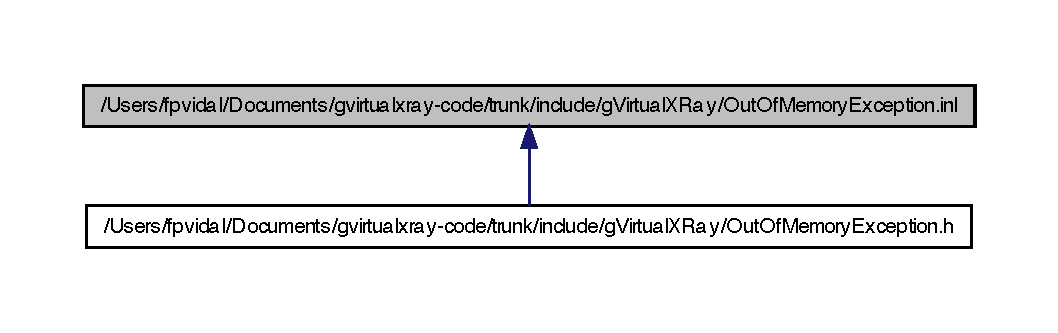
\includegraphics[width=400pt]{_out_of_memory_exception_8inl__dep__incl}
\end{center}
\end{figure}
\subsection*{Namespaces}
\begin{DoxyCompactItemize}
\item 
namespace \hyperlink{namespace_utilities}{Utilities}
\end{DoxyCompactItemize}


\subsection{Detailed Description}
Class to handle exceptions when memory cannot be allocated dynamically. \begin{DoxyVersion}{Version}
1.0
\end{DoxyVersion}
\begin{DoxyDate}{Date}
30/11/2013
\end{DoxyDate}
\begin{DoxyAuthor}{Author}
Dr Franck P. Vidal
\end{DoxyAuthor}
\hypertarget{_x_ray_renderer_8inl_License}{}\subsection{License}\label{_x_ray_renderer_8inl_License}
BSD 3-\/Clause License.

For details on use and redistribution please refer to \href{http://opensource.org/licenses/BSD-3-Clause}{\tt http://opensource.org/licenses/BSD-\/3-\/Clause}\hypertarget{_x_ray_renderer_8inl_Copyright}{}\subsection{Copyright}\label{_x_ray_renderer_8inl_Copyright}
(c) by Dr Franck P. Vidal (\href{mailto:franck.p.vidal@fpvidal.net}{\tt franck.p.vidal@fpvidal.net}), \href{http://www.fpvidal.net/,}{\tt http://www.fpvidal.net/,} Dec 2013, 2013, version 1.0, BSD 3-\/Clause License 

Definition in file \hyperlink{_out_of_memory_exception_8inl_source}{OutOfMemoryException.inl}.


\hypertarget{_polygon_mesh_8h}{
\section{/Users/fpvidal/Documents/gvirtualxray-\/code/trunk/include/gVirtualXRay/PolygonMesh.h File Reference}
\label{_polygon_mesh_8h}\index{/Users/fpvidal/Documents/gvirtualxray-\/code/trunk/include/gVirtualXRay/PolygonMesh.h@{/Users/fpvidal/Documents/gvirtualxray-\/code/trunk/include/gVirtualXRay/PolygonMesh.h}}
}


Class to handle polygon (triangles or quads) meshes.  


{\ttfamily \#include $<$string$>$}\par
{\ttfamily \#include $<$vector$>$}\par
{\ttfamily \#include \char`\"{}gVirtualXRay/VBO.h\char`\"{}}\par
{\ttfamily \#include \char`\"{}gVirtualXRay/Types.h\char`\"{}}\par
{\ttfamily \#include \char`\"{}gVirtualXRay/Units.h\char`\"{}}\par
{\ttfamily \#include \char`\"{}PolygonMesh.inl\char`\"{}}\par
Include dependency graph for PolygonMesh.h:
\nopagebreak
\begin{figure}[H]
\begin{center}
\leavevmode
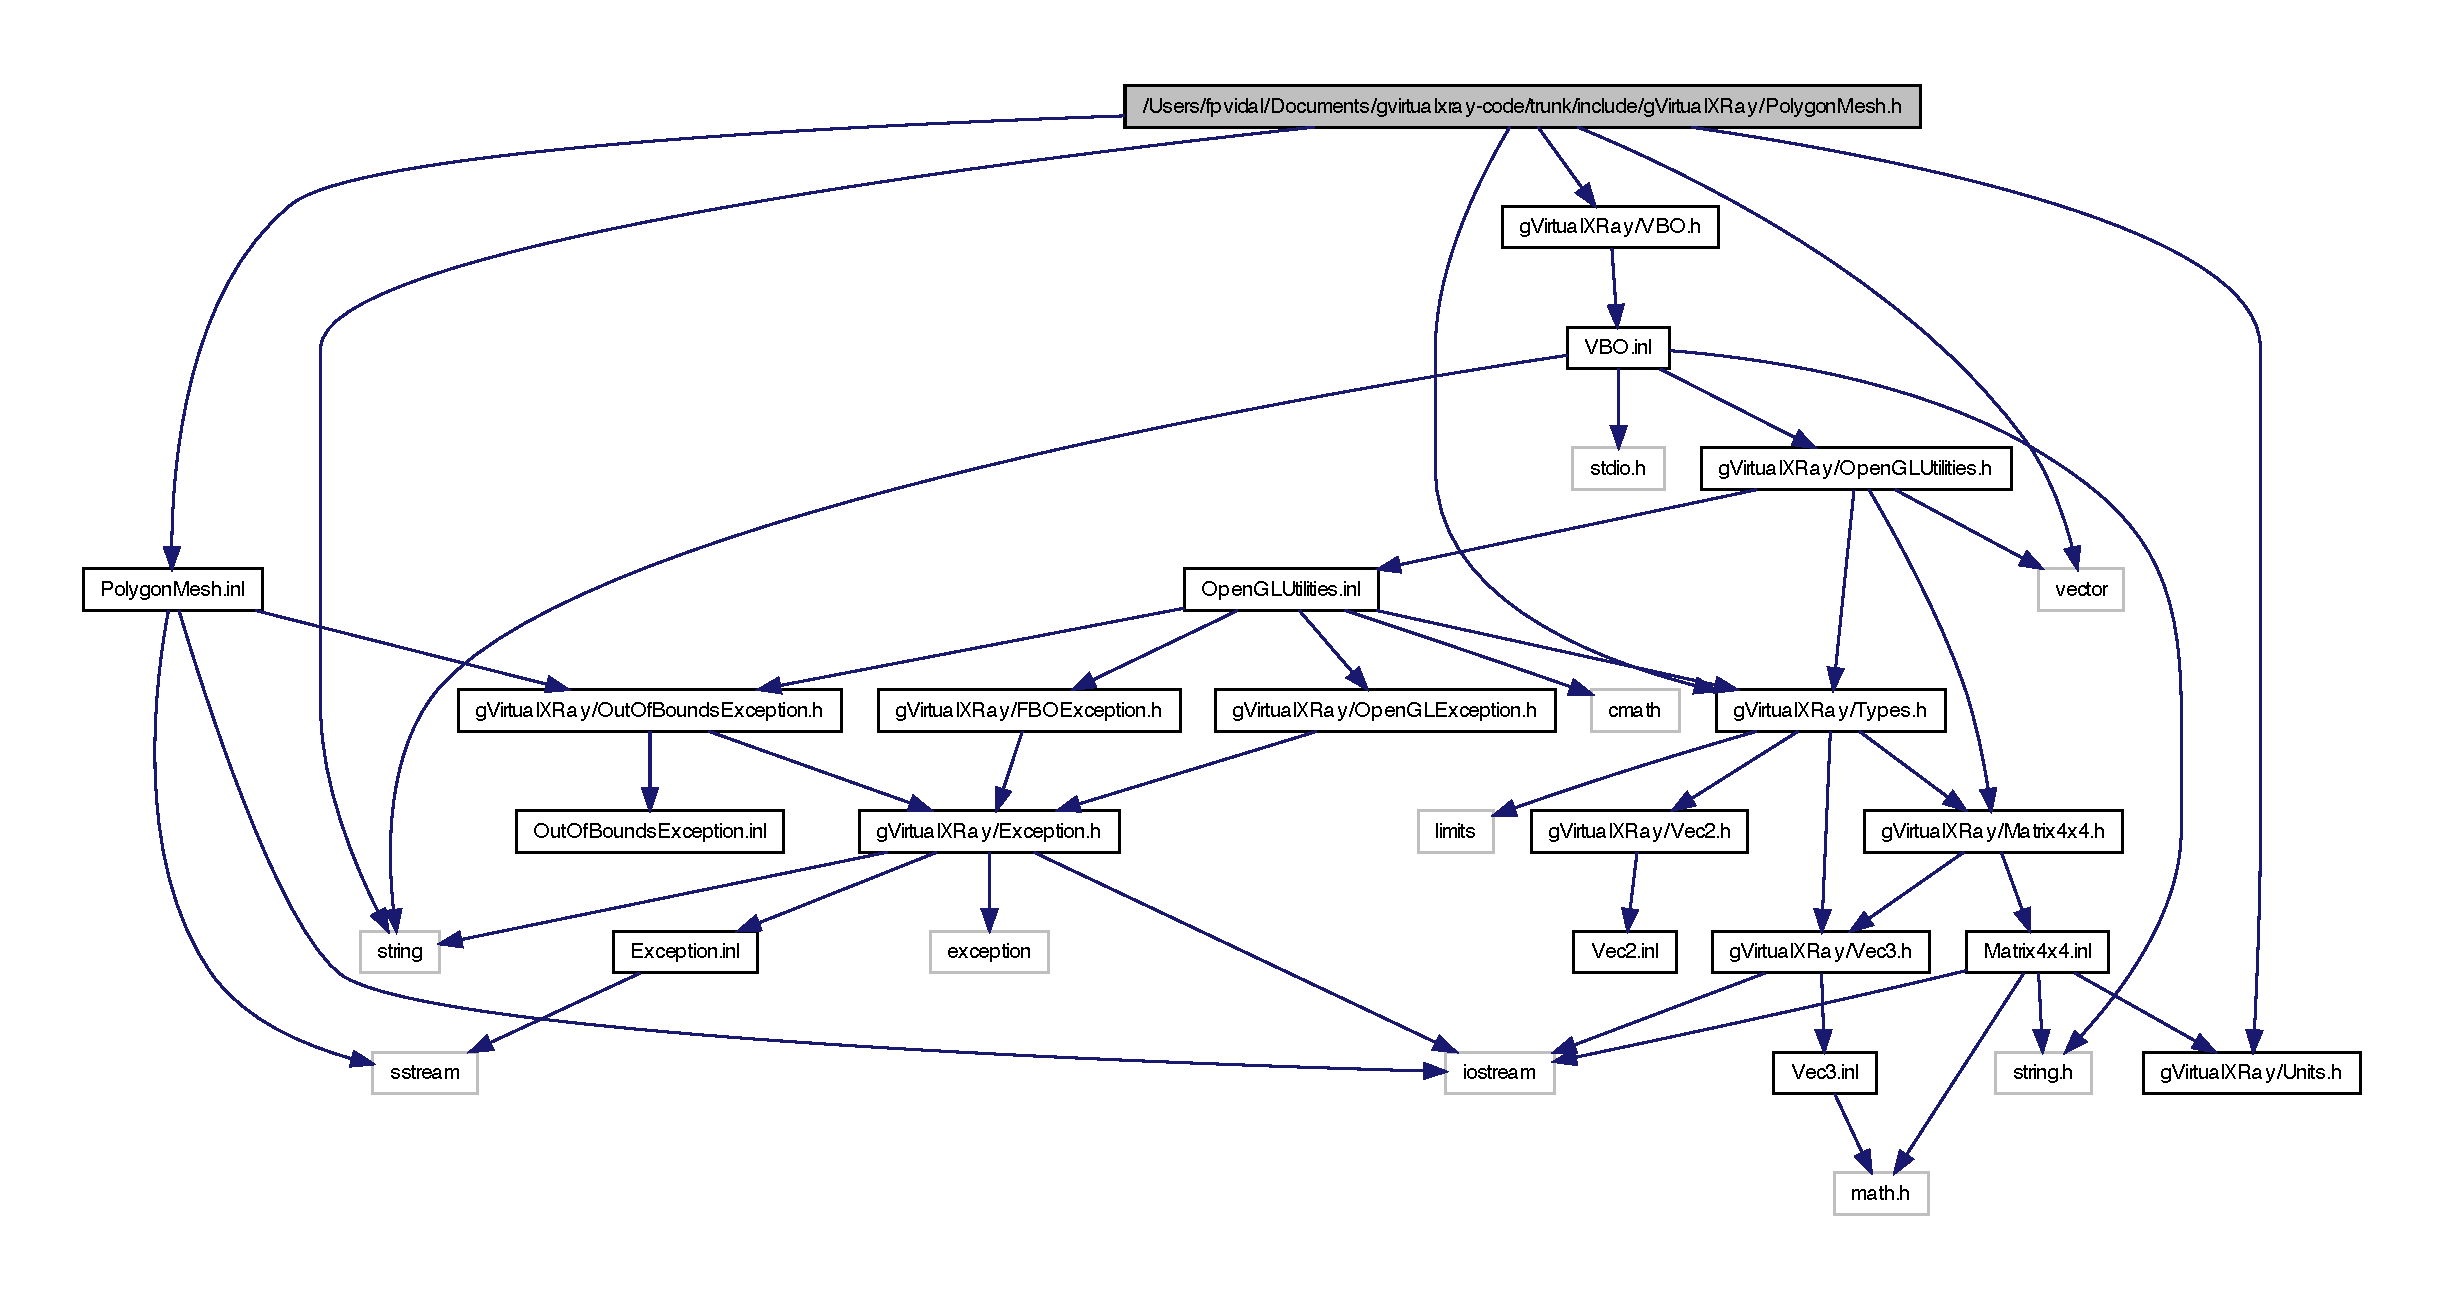
\includegraphics[width=400pt]{_polygon_mesh_8h__incl}
\end{center}
\end{figure}
This graph shows which files directly or indirectly include this file:
\nopagebreak
\begin{figure}[H]
\begin{center}
\leavevmode
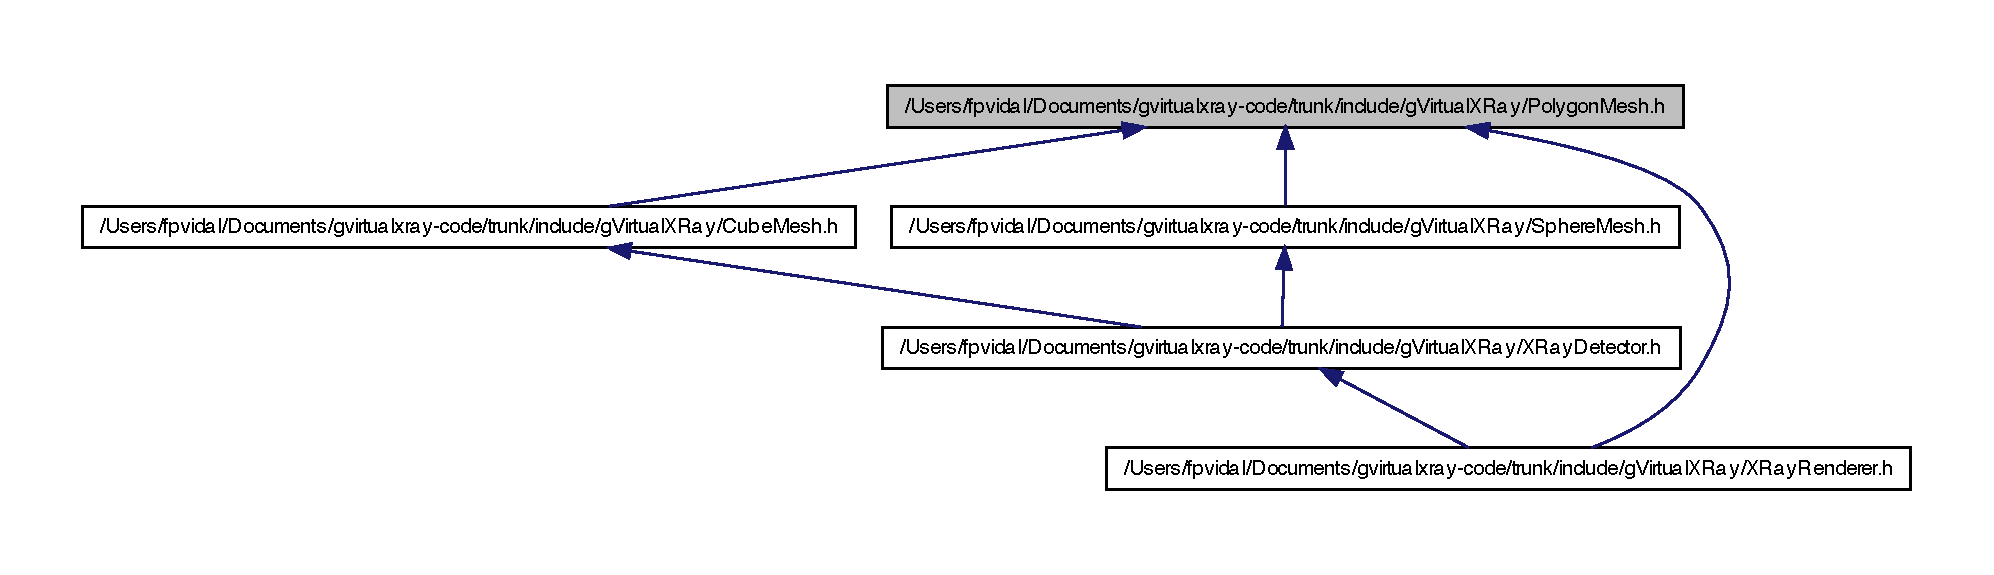
\includegraphics[width=400pt]{_polygon_mesh_8h__dep__incl}
\end{center}
\end{figure}
\subsection*{Classes}
\begin{DoxyCompactItemize}
\item 
class \hyperlink{class_graphics_1_1_polygon_mesh}{Graphics::PolygonMesh}
\begin{DoxyCompactList}\small\item\em \hyperlink{class_graphics_1_1_polygon_mesh}{PolygonMesh} is a class to handle polygon (triangles or quads) meshes. \end{DoxyCompactList}\end{DoxyCompactItemize}
\subsection*{Namespaces}
\begin{DoxyCompactItemize}
\item 
namespace \hyperlink{namespace_graphics}{Graphics}
\end{DoxyCompactItemize}


\subsection{Detailed Description}
Class to handle polygon (triangles or quads) meshes. \begin{DoxyVersion}{Version}
1.0
\end{DoxyVersion}
\begin{DoxyDate}{Date}
07/11/2013
\end{DoxyDate}
\begin{DoxyAuthor}{Author}
Dr Franck P. Vidal
\end{DoxyAuthor}
\begin{Desc}
\item[\hyperlink{todo__todo000003}{Todo}]Make it possible to merge vertices if an array of indices exists Convert triangle mesh into arbitrary polygon mesh\end{Desc}
\hypertarget{_x_ray_renderer_8inl_License}{}\subsection{License}\label{_x_ray_renderer_8inl_License}
BSD 3-\/Clause License.

For details on use and redistribution please refer to \href{http://opensource.org/licenses/BSD-3-Clause}{\tt http://opensource.org/licenses/BSD-\/3-\/Clause}\hypertarget{_x_ray_renderer_8inl_Copyright}{}\subsection{Copyright}\label{_x_ray_renderer_8inl_Copyright}
(c) by Dr Franck P. Vidal (\href{mailto:franck.p.vidal@fpvidal.net}{\tt franck.p.vidal@fpvidal.net}), \href{http://www.fpvidal.net/,}{\tt http://www.fpvidal.net/,} Dec 2013, 2013, version 1.0, BSD 3-\/Clause License 

Definition in file \hyperlink{_polygon_mesh_8h_source}{PolygonMesh.h}.


\hypertarget{_polygon_mesh_8inl}{
\section{/Users/fpvidal/Documents/gvirtualxray-\/code/trunk/include/gVirtualXRay/PolygonMesh.inl File Reference}
\label{_polygon_mesh_8inl}\index{/Users/fpvidal/Documents/gvirtualxray-\/code/trunk/include/gVirtualXRay/PolygonMesh.inl@{/Users/fpvidal/Documents/gvirtualxray-\/code/trunk/include/gVirtualXRay/PolygonMesh.inl}}
}


Class to handle polygon (triangles or quads) meshes.  


{\ttfamily \#include $<$iostream$>$}\par
{\ttfamily \#include $<$sstream$>$}\par
{\ttfamily \#include \char`\"{}gVirtualXRay/OutOfBoundsException.h\char`\"{}}\par
Include dependency graph for PolygonMesh.inl:
\nopagebreak
\begin{figure}[H]
\begin{center}
\leavevmode
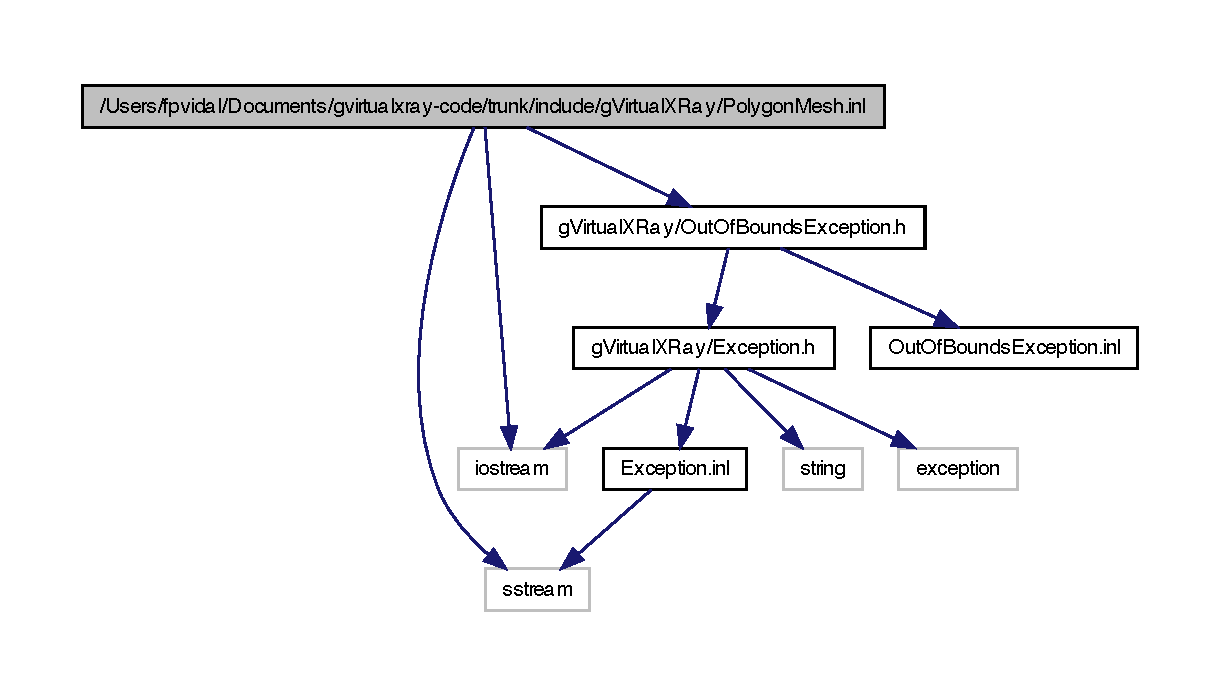
\includegraphics[width=400pt]{_polygon_mesh_8inl__incl}
\end{center}
\end{figure}
This graph shows which files directly or indirectly include this file:
\nopagebreak
\begin{figure}[H]
\begin{center}
\leavevmode
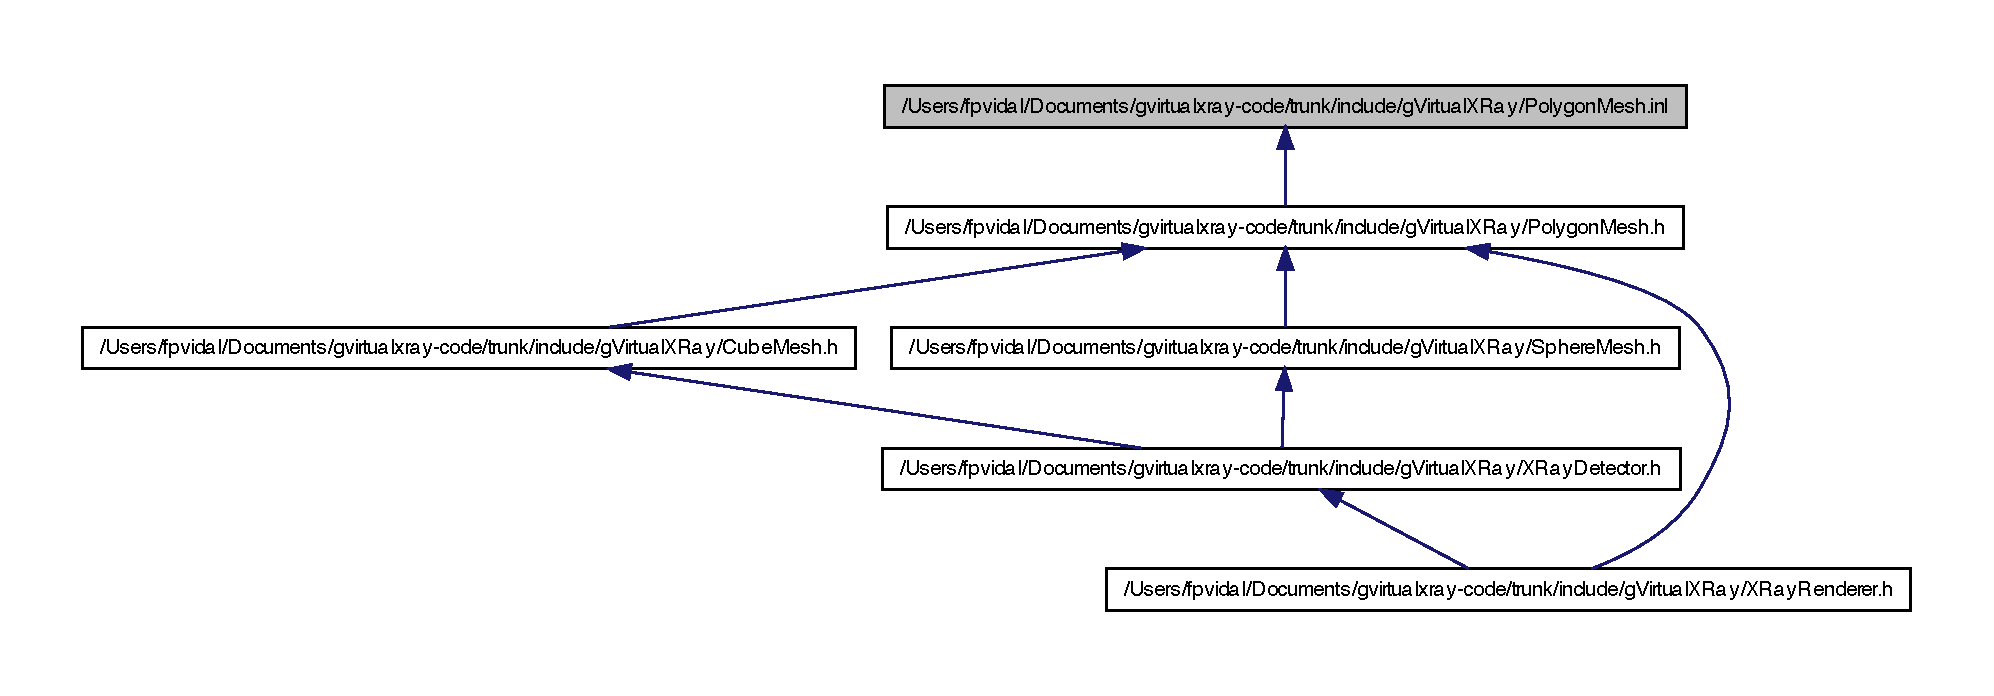
\includegraphics[width=400pt]{_polygon_mesh_8inl__dep__incl}
\end{center}
\end{figure}
\subsection*{Namespaces}
\begin{DoxyCompactItemize}
\item 
namespace \hyperlink{namespace_graphics}{Graphics}
\end{DoxyCompactItemize}


\subsection{Detailed Description}
Class to handle polygon (triangles or quads) meshes. \begin{DoxyVersion}{Version}
1.0
\end{DoxyVersion}
\begin{DoxyDate}{Date}
07/11/2013
\end{DoxyDate}
\begin{DoxyAuthor}{Author}
Dr Franck P. Vidal
\end{DoxyAuthor}
\hypertarget{_x_ray_renderer_8inl_License}{}\subsection{License}\label{_x_ray_renderer_8inl_License}
BSD 3-\/Clause License.

For details on use and redistribution please refer to \href{http://opensource.org/licenses/BSD-3-Clause}{\tt http://opensource.org/licenses/BSD-\/3-\/Clause}\hypertarget{_x_ray_renderer_8inl_Copyright}{}\subsection{Copyright}\label{_x_ray_renderer_8inl_Copyright}
(c) by Dr Franck P. Vidal (\href{mailto:franck.p.vidal@fpvidal.net}{\tt franck.p.vidal@fpvidal.net}), \href{http://www.fpvidal.net/,}{\tt http://www.fpvidal.net/,} Dec 2013, 2013, version 1.0, BSD 3-\/Clause License 

Definition in file \hyperlink{_polygon_mesh_8inl_source}{PolygonMesh.inl}.


\hypertarget{_shader_8h}{
\section{/Users/fpvidal/Documents/gvirtualxray-\/code/trunk/include/gVirtualXRay/Shader.h File Reference}
\label{_shader_8h}\index{/Users/fpvidal/Documents/gvirtualxray-\/code/trunk/include/gVirtualXRay/Shader.h@{/Users/fpvidal/Documents/gvirtualxray-\/code/trunk/include/gVirtualXRay/Shader.h}}
}


Class to handle GLSL shaders.  


{\ttfamily \#include $<$string$>$}\par
{\ttfamily \#include \char`\"{}Shader.inl\char`\"{}}\par
Include dependency graph for Shader.h:\nopagebreak
\begin{figure}[H]
\begin{center}
\leavevmode
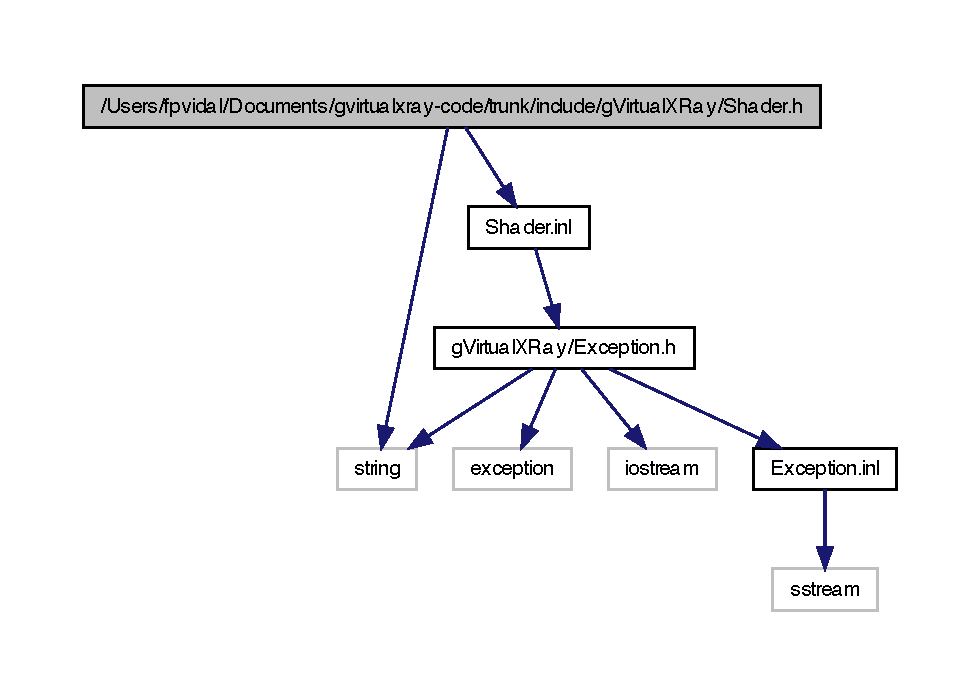
\includegraphics[width=400pt]{_shader_8h__incl}
\end{center}
\end{figure}
This graph shows which files directly or indirectly include this file:\nopagebreak
\begin{figure}[H]
\begin{center}
\leavevmode
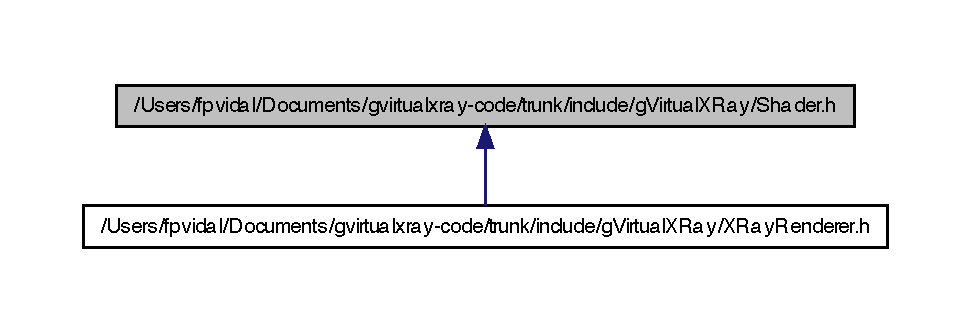
\includegraphics[width=400pt]{_shader_8h__dep__incl}
\end{center}
\end{figure}
\subsection*{Classes}
\begin{DoxyCompactItemize}
\item 
class \hyperlink{class_graphics_1_1_shader}{Graphics::Shader}
\begin{DoxyCompactList}\small\item\em \hyperlink{class_graphics_1_1_shader}{Shader} is a class to handle shaders written in GLSL. \end{DoxyCompactList}\end{DoxyCompactItemize}
\subsection*{Namespaces}
\begin{DoxyCompactItemize}
\item 
namespace \hyperlink{namespace_graphics}{Graphics}
\end{DoxyCompactItemize}


\subsection{Detailed Description}
Class to handle GLSL shaders. \begin{DoxyVersion}{Version}
1.0
\end{DoxyVersion}
\begin{DoxyDate}{Date}
29/11/2013
\end{DoxyDate}
\begin{DoxyAuthor}{Author}
Dr Franck P. Vidal
\end{DoxyAuthor}
\hypertarget{_x_ray_renderer_8inl_License}{}\subsection{License}\label{_x_ray_renderer_8inl_License}
BSD 3-\/Clause License.

For details on use and redistribution please refer to \href{http://opensource.org/licenses/BSD-3-Clause}{\tt http://opensource.org/licenses/BSD-\/3-\/Clause}\hypertarget{_x_ray_renderer_8inl_Copyright}{}\subsection{Copyright}\label{_x_ray_renderer_8inl_Copyright}
(c) by Dr Franck P. Vidal (\href{mailto:franck.p.vidal@fpvidal.net}{\tt franck.p.vidal@fpvidal.net}), \href{http://www.fpvidal.net/,}{\tt http://www.fpvidal.net/,} Dec 2013, 2013, version 1.0, BSD 3-\/Clause License 

Definition in file \hyperlink{_shader_8h_source}{Shader.h}.


\hypertarget{_shader_8inl}{
\section{/Users/fpvidal/Documents/gvirtualxray-\/code/trunk/include/gVirtualXRay/Shader.inl File Reference}
\label{_shader_8inl}\index{/Users/fpvidal/Documents/gvirtualxray-\/code/trunk/include/gVirtualXRay/Shader.inl@{/Users/fpvidal/Documents/gvirtualxray-\/code/trunk/include/gVirtualXRay/Shader.inl}}
}


Class to handle GLSL shaders.  


{\ttfamily \#include \char`\"{}gVirtualXRay/Exception.h\char`\"{}}\par
Include dependency graph for Shader.inl:\nopagebreak
\begin{figure}[H]
\begin{center}
\leavevmode
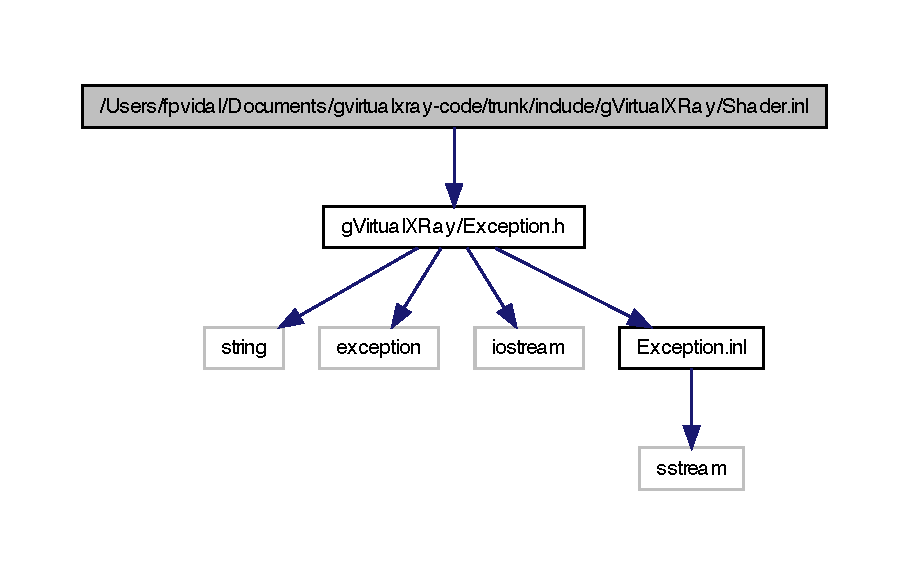
\includegraphics[width=400pt]{_shader_8inl__incl}
\end{center}
\end{figure}
This graph shows which files directly or indirectly include this file:\nopagebreak
\begin{figure}[H]
\begin{center}
\leavevmode
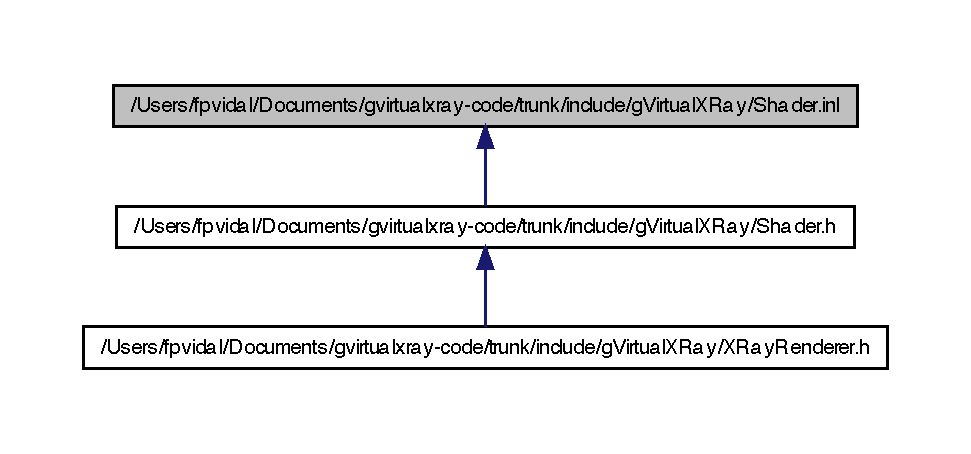
\includegraphics[width=400pt]{_shader_8inl__dep__incl}
\end{center}
\end{figure}
\subsection*{Namespaces}
\begin{DoxyCompactItemize}
\item 
namespace \hyperlink{namespace_graphics}{Graphics}
\end{DoxyCompactItemize}


\subsection{Detailed Description}
Class to handle GLSL shaders. \begin{DoxyVersion}{Version}
1.0
\end{DoxyVersion}
\begin{DoxyDate}{Date}
29/11/2013
\end{DoxyDate}
\begin{DoxyAuthor}{Author}
Dr Franck P. Vidal
\end{DoxyAuthor}
\hypertarget{_x_ray_renderer_8inl_License}{}\subsection{License}\label{_x_ray_renderer_8inl_License}
BSD 3-\/Clause License.

For details on use and redistribution please refer to \href{http://opensource.org/licenses/BSD-3-Clause}{\tt http://opensource.org/licenses/BSD-\/3-\/Clause}\hypertarget{_x_ray_renderer_8inl_Copyright}{}\subsection{Copyright}\label{_x_ray_renderer_8inl_Copyright}
(c) by Dr Franck P. Vidal (\href{mailto:franck.p.vidal@fpvidal.net}{\tt franck.p.vidal@fpvidal.net}), \href{http://www.fpvidal.net/,}{\tt http://www.fpvidal.net/,} Dec 2013, 2013, version 1.0, BSD 3-\/Clause License 

Definition in file \hyperlink{_shader_8inl_source}{Shader.inl}.


\hypertarget{_spectrum_record_8h}{
\section{/Users/fpvidal/Documents/gvirtualxray-\/code/trunk/include/gVirtualXRay/SpectrumRecord.h File Reference}
\label{_spectrum_record_8h}\index{/Users/fpvidal/Documents/gvirtualxray-\/code/trunk/include/gVirtualXRay/SpectrumRecord.h@{/Users/fpvidal/Documents/gvirtualxray-\/code/trunk/include/gVirtualXRay/SpectrumRecord.h}}
}


Class to manage a record of the X-\/Ray beam, i.e. an energy bin (number of photons, energy of the photons in the bin).  


{\ttfamily \#include $<$iostream$>$}\par
{\ttfamily \#include \char`\"{}gVirtualXRay/Types.h\char`\"{}}\par
{\ttfamily \#include \char`\"{}SpectrumRecord.inl\char`\"{}}\par
Include dependency graph for SpectrumRecord.h:\nopagebreak
\begin{figure}[H]
\begin{center}
\leavevmode
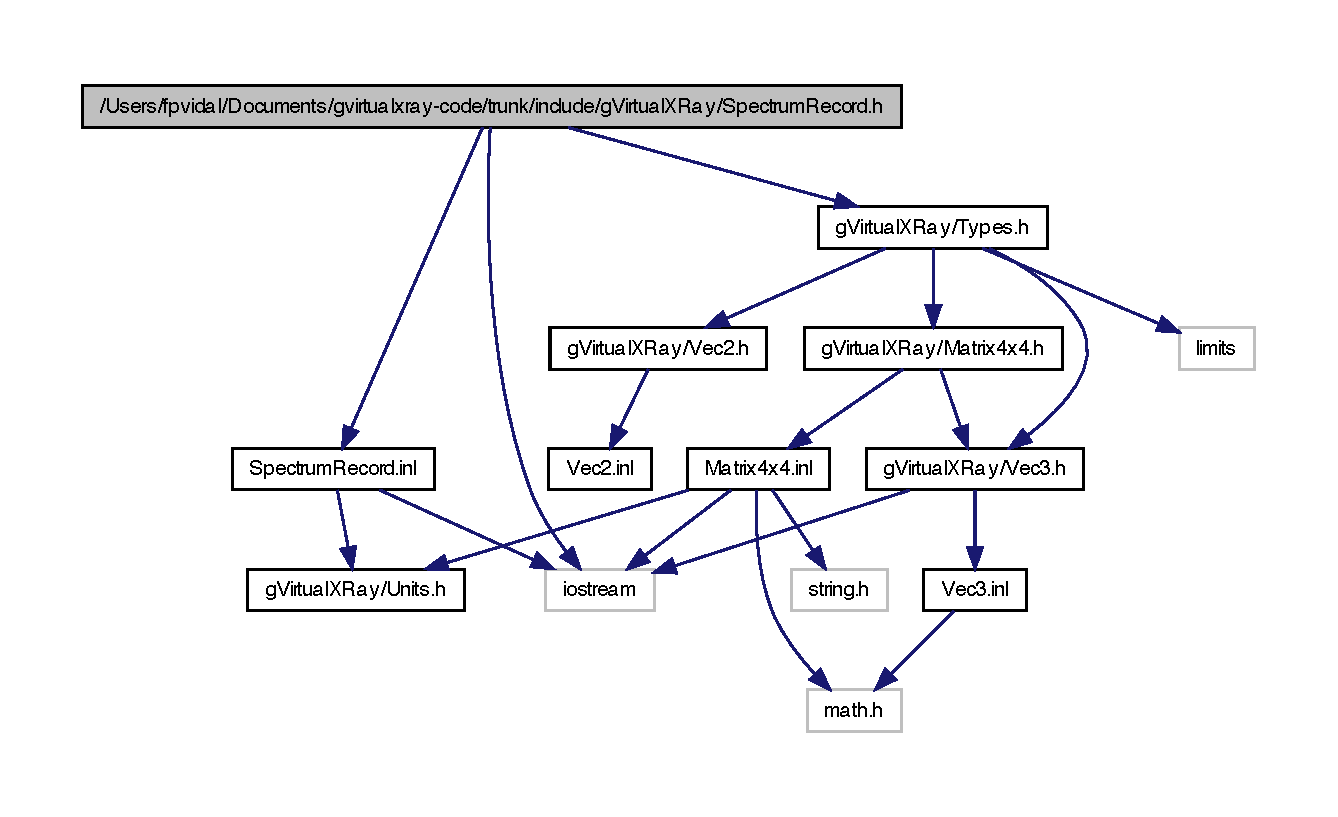
\includegraphics[width=400pt]{_spectrum_record_8h__incl}
\end{center}
\end{figure}
This graph shows which files directly or indirectly include this file:\nopagebreak
\begin{figure}[H]
\begin{center}
\leavevmode
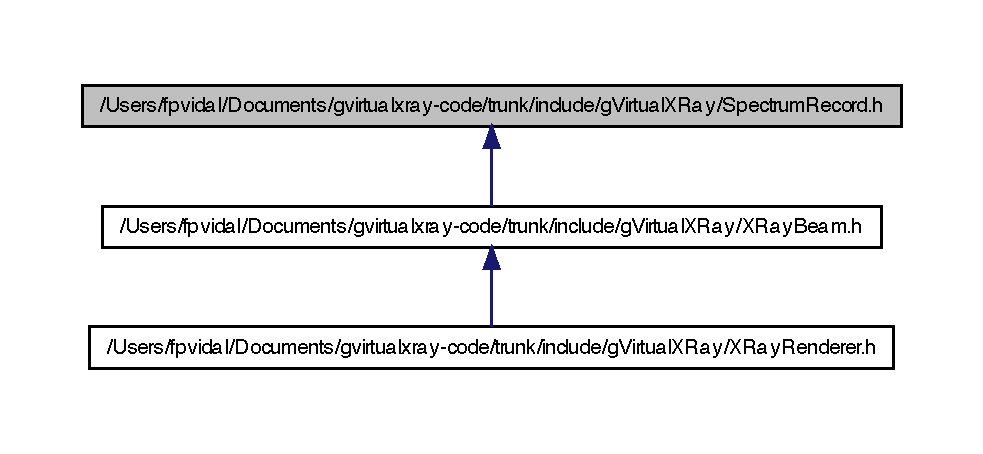
\includegraphics[width=400pt]{_spectrum_record_8h__dep__incl}
\end{center}
\end{figure}
\subsection*{Classes}
\begin{DoxyCompactItemize}
\item 
class \hyperlink{classg_virtual_x_ray_1_1_spectrum_record}{gVirtualXRay::SpectrumRecord}
\begin{DoxyCompactList}\small\item\em \hyperlink{classg_virtual_x_ray_1_1_spectrum_record}{SpectrumRecord} is a class to handle a record of the X-\/Ray beam, i.e. an energy bin (number of photons, energy of the photons in the bin). \end{DoxyCompactList}\end{DoxyCompactItemize}
\subsection*{Namespaces}
\begin{DoxyCompactItemize}
\item 
namespace \hyperlink{namespaceg_virtual_x_ray}{gVirtualXRay}
\end{DoxyCompactItemize}
\subsection*{Functions}
\begin{DoxyCompactItemize}
\item 
std::istream \& \hyperlink{namespaceg_virtual_x_ray_a46753e0c9aaf9a9a041dc0a5d3e946b2}{gVirtualXRay::operator$>$$>$} (std::istream \&is, SpectrumRecord \&obj)
\begin{DoxyCompactList}\small\item\em operator$>$$>$ \end{DoxyCompactList}\item 
std::ostream \& \hyperlink{namespaceg_virtual_x_ray_ae67e9f780e259aa1a6af681661155020}{gVirtualXRay::operator$<$$<$} (std::ostream \&os, const SpectrumRecord \&obj)
\begin{DoxyCompactList}\small\item\em operator$<$$<$ \end{DoxyCompactList}\end{DoxyCompactItemize}


\subsection{Detailed Description}
Class to manage a record of the X-\/Ray beam, i.e. an energy bin (number of photons, energy of the photons in the bin). \begin{DoxyVersion}{Version}
1.0
\end{DoxyVersion}
\begin{DoxyDate}{Date}
30/11/2013
\end{DoxyDate}
\begin{DoxyAuthor}{Author}
Dr Franck P. Vidal
\end{DoxyAuthor}
\hypertarget{_x_ray_renderer_8inl_License}{}\subsection{License}\label{_x_ray_renderer_8inl_License}
BSD 3-\/Clause License.

For details on use and redistribution please refer to \href{http://opensource.org/licenses/BSD-3-Clause}{\tt http://opensource.org/licenses/BSD-\/3-\/Clause}\hypertarget{_x_ray_renderer_8inl_Copyright}{}\subsection{Copyright}\label{_x_ray_renderer_8inl_Copyright}
(c) by Dr Franck P. Vidal (\href{mailto:franck.p.vidal@fpvidal.net}{\tt franck.p.vidal@fpvidal.net}), \href{http://www.fpvidal.net/,}{\tt http://www.fpvidal.net/,} Dec 2013, 2013, version 1.0, BSD 3-\/Clause License 

Definition in file \hyperlink{_spectrum_record_8h_source}{SpectrumRecord.h}.


\hypertarget{_spectrum_record_8inl}{
\section{/Users/fpvidal/Documents/gvirtualxray-\/code/trunk/include/gVirtualXRay/SpectrumRecord.inl File Reference}
\label{_spectrum_record_8inl}\index{/Users/fpvidal/Documents/gvirtualxray-\/code/trunk/include/gVirtualXRay/SpectrumRecord.inl@{/Users/fpvidal/Documents/gvirtualxray-\/code/trunk/include/gVirtualXRay/SpectrumRecord.inl}}
}


Class to manage a record of the X-\/Ray beam, i.e. an energy bin (number of photons, energy of the photons in the bin).  


{\ttfamily \#include $<$iostream$>$}\par
{\ttfamily \#include \char`\"{}gVirtualXRay/Units.h\char`\"{}}\par
Include dependency graph for SpectrumRecord.inl:\nopagebreak
\begin{figure}[H]
\begin{center}
\leavevmode
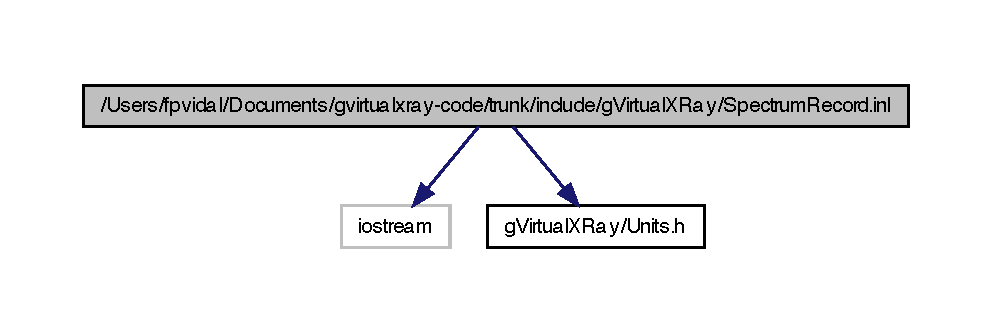
\includegraphics[width=400pt]{_spectrum_record_8inl__incl}
\end{center}
\end{figure}
This graph shows which files directly or indirectly include this file:\nopagebreak
\begin{figure}[H]
\begin{center}
\leavevmode
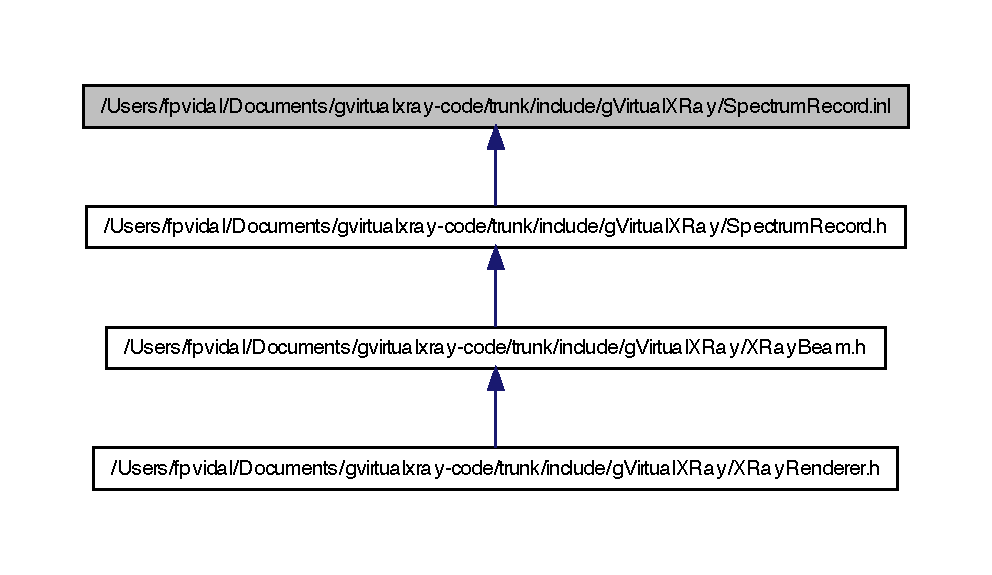
\includegraphics[width=400pt]{_spectrum_record_8inl__dep__incl}
\end{center}
\end{figure}
\subsection*{Namespaces}
\begin{DoxyCompactItemize}
\item 
namespace \hyperlink{namespaceg_virtual_x_ray}{gVirtualXRay}
\end{DoxyCompactItemize}
\subsection*{Functions}
\begin{DoxyCompactItemize}
\item 
std::istream \& \hyperlink{namespaceg_virtual_x_ray_a46753e0c9aaf9a9a041dc0a5d3e946b2}{gVirtualXRay::operator$>$$>$} (std::istream \&is, SpectrumRecord \&obj)
\begin{DoxyCompactList}\small\item\em operator$>$$>$ \end{DoxyCompactList}\item 
std::ostream \& \hyperlink{namespaceg_virtual_x_ray_ae67e9f780e259aa1a6af681661155020}{gVirtualXRay::operator$<$$<$} (std::ostream \&os, const SpectrumRecord \&obj)
\begin{DoxyCompactList}\small\item\em operator$<$$<$ \end{DoxyCompactList}\end{DoxyCompactItemize}


\subsection{Detailed Description}
Class to manage a record of the X-\/Ray beam, i.e. an energy bin (number of photons, energy of the photons in the bin). \begin{DoxyVersion}{Version}
1.0
\end{DoxyVersion}
\begin{DoxyDate}{Date}
30/11/2013
\end{DoxyDate}
\begin{DoxyAuthor}{Author}
Dr Franck P. Vidal
\end{DoxyAuthor}
\hypertarget{_x_ray_renderer_8inl_License}{}\subsection{License}\label{_x_ray_renderer_8inl_License}
BSD 3-\/Clause License.

For details on use and redistribution please refer to \href{http://opensource.org/licenses/BSD-3-Clause}{\tt http://opensource.org/licenses/BSD-\/3-\/Clause}\hypertarget{_x_ray_renderer_8inl_Copyright}{}\subsection{Copyright}\label{_x_ray_renderer_8inl_Copyright}
(c) by Dr Franck P. Vidal (\href{mailto:franck.p.vidal@fpvidal.net}{\tt franck.p.vidal@fpvidal.net}), \href{http://www.fpvidal.net/,}{\tt http://www.fpvidal.net/,} Dec 2013, 2013, version 1.0, BSD 3-\/Clause License 

Definition in file \hyperlink{_spectrum_record_8inl_source}{SpectrumRecord.inl}.


\hypertarget{_sphere_mesh_8h}{
\section{/Users/fpvidal/Documents/gvirtualxray-\/code/trunk/include/gVirtualXRay/SphereMesh.h File Reference}
\label{_sphere_mesh_8h}\index{/Users/fpvidal/Documents/gvirtualxray-\/code/trunk/include/gVirtualXRay/SphereMesh.h@{/Users/fpvidal/Documents/gvirtualxray-\/code/trunk/include/gVirtualXRay/SphereMesh.h}}
}


Class to handle 3D meshes of spheres.  


{\ttfamily \#include $<$string$>$}\par
{\ttfamily \#include $<$vector$>$}\par
{\ttfamily \#include \char`\"{}gVirtualXRay/PolygonMesh.h\char`\"{}}\par
{\ttfamily \#include \char`\"{}gVirtualXRay/Types.h\char`\"{}}\par
{\ttfamily \#include \char`\"{}SphereMesh.inl\char`\"{}}\par
Include dependency graph for SphereMesh.h:
\nopagebreak
\begin{figure}[H]
\begin{center}
\leavevmode
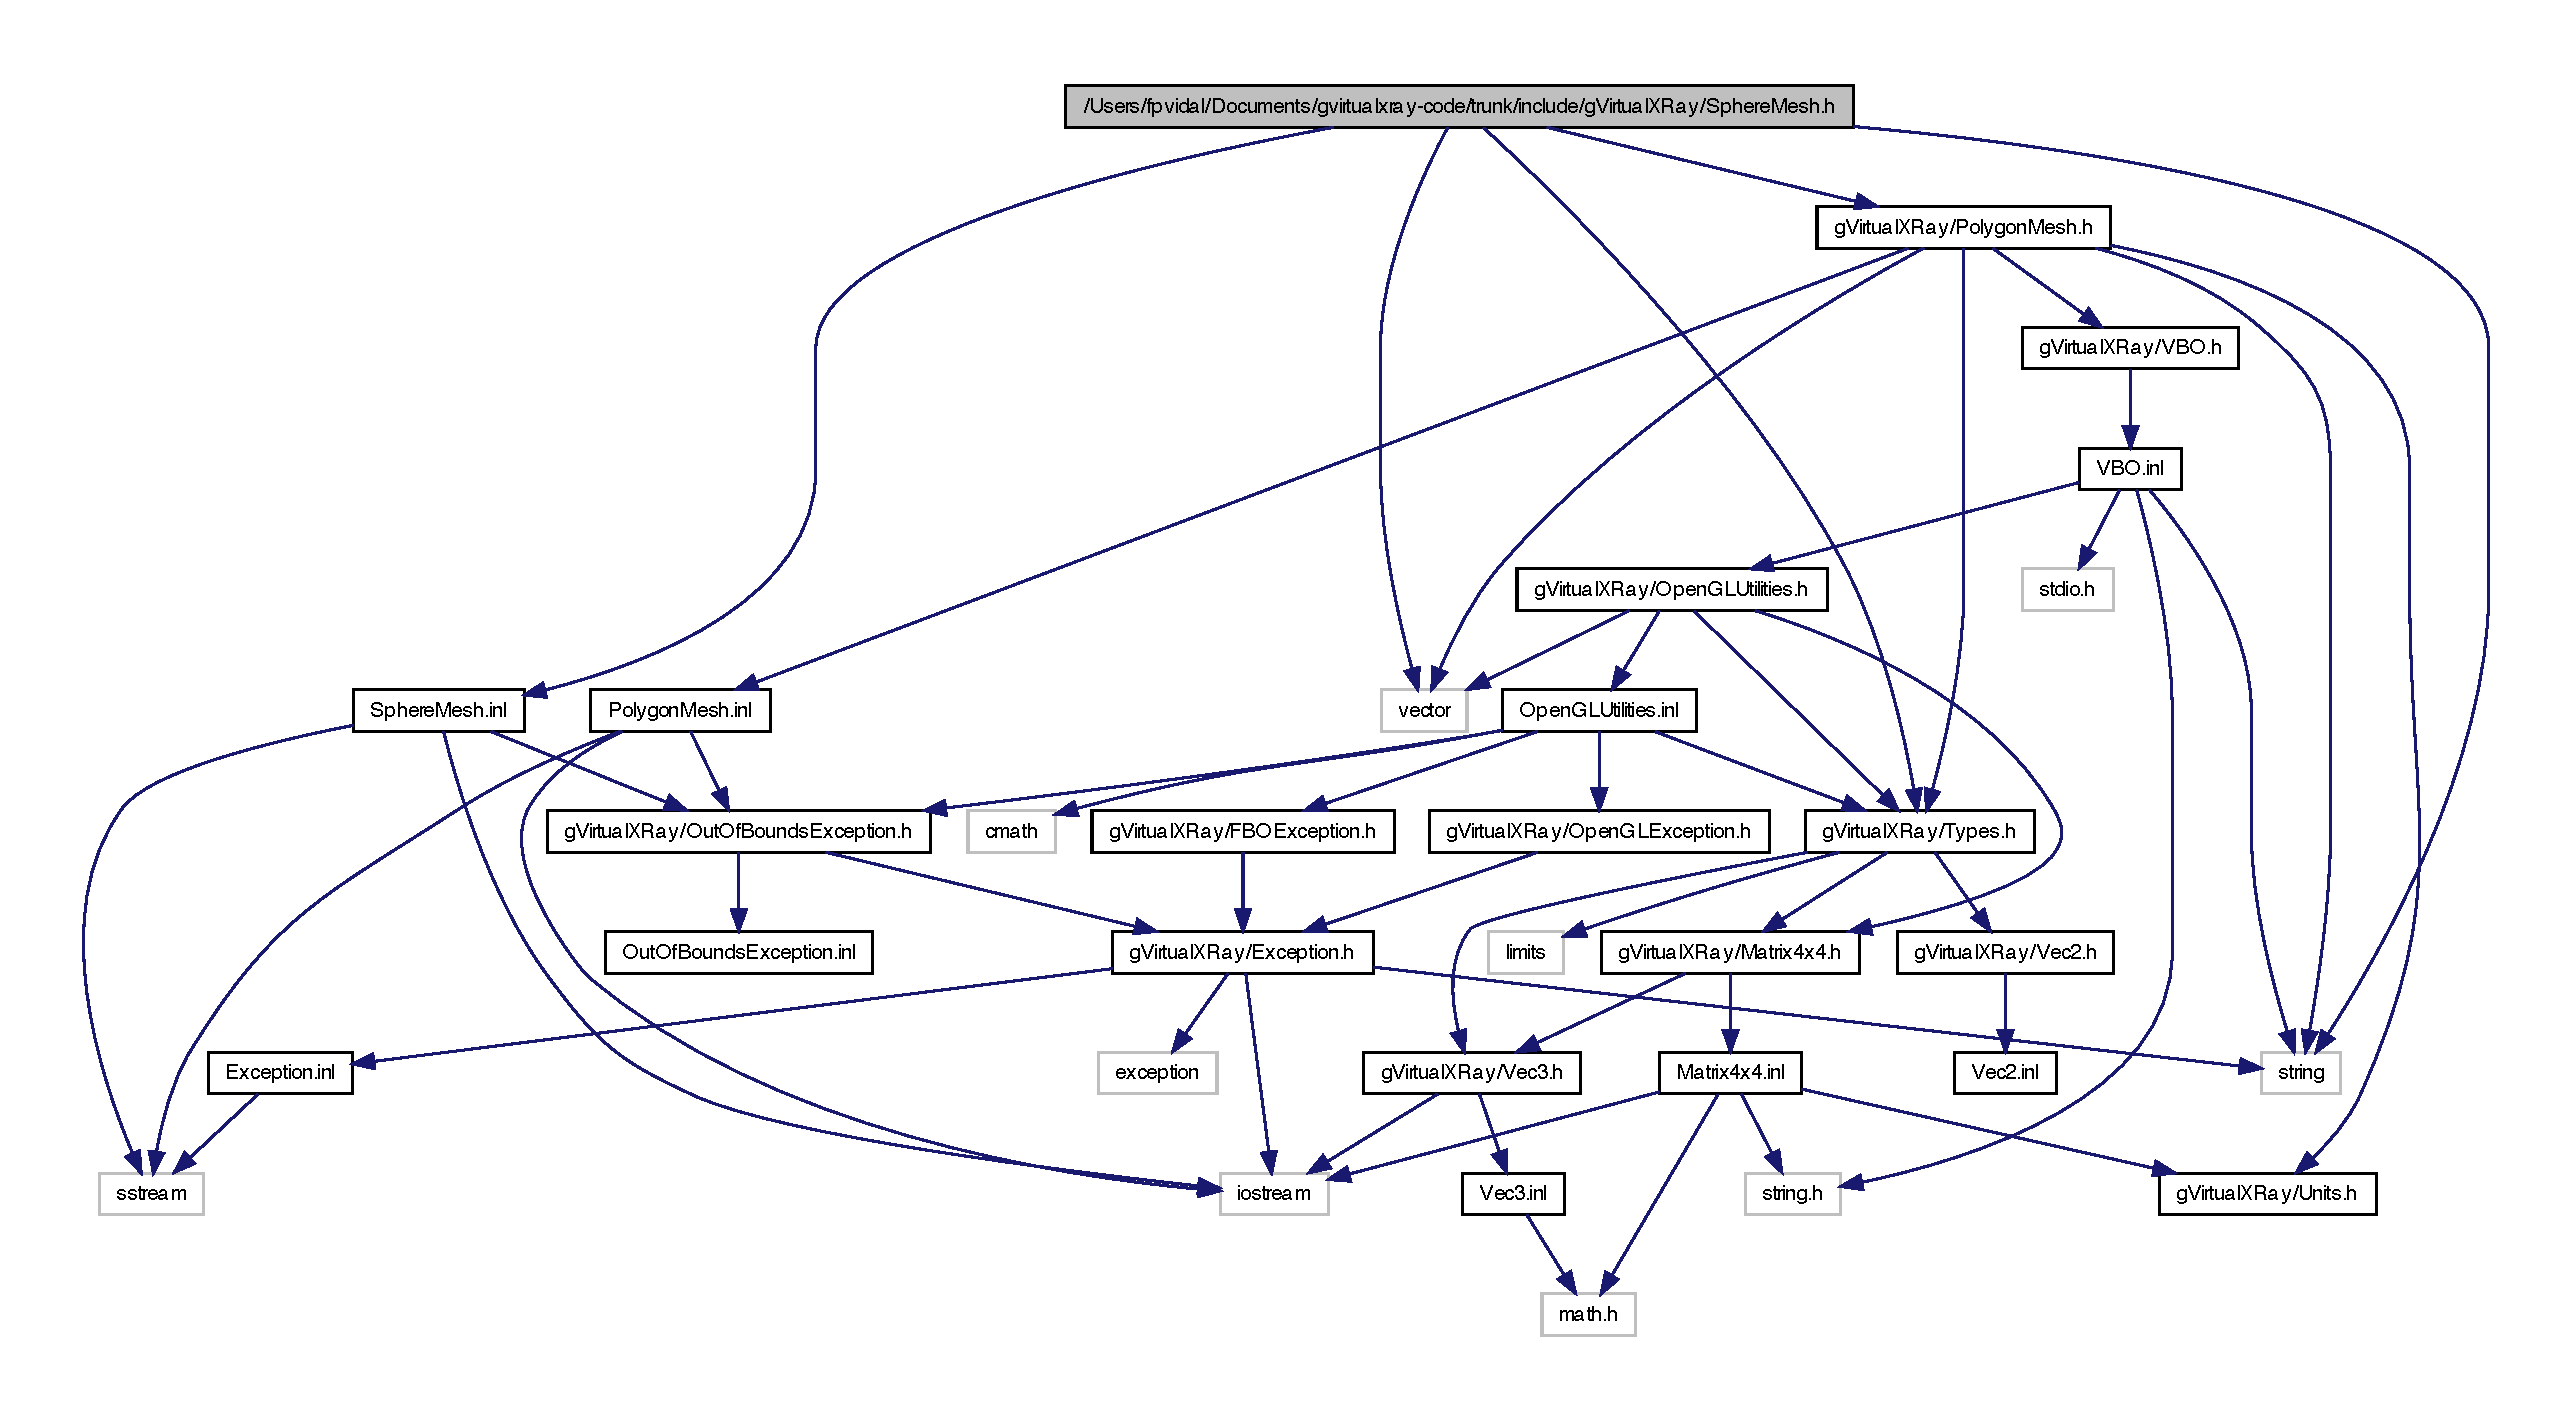
\includegraphics[width=400pt]{_sphere_mesh_8h__incl}
\end{center}
\end{figure}
This graph shows which files directly or indirectly include this file:\nopagebreak
\begin{figure}[H]
\begin{center}
\leavevmode
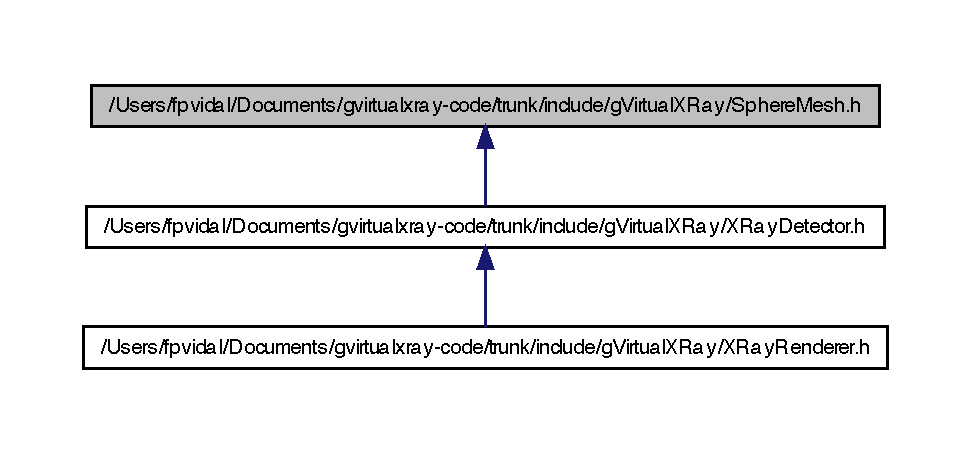
\includegraphics[width=400pt]{_sphere_mesh_8h__dep__incl}
\end{center}
\end{figure}
\subsection*{Classes}
\begin{DoxyCompactItemize}
\item 
class \hyperlink{class_graphics_1_1_sphere_mesh}{Graphics::SphereMesh}
\begin{DoxyCompactList}\small\item\em \hyperlink{class_graphics_1_1_sphere_mesh}{SphereMesh} is a class to handle 3D meshes of spheres. \end{DoxyCompactList}\end{DoxyCompactItemize}
\subsection*{Namespaces}
\begin{DoxyCompactItemize}
\item 
namespace \hyperlink{namespace_graphics}{Graphics}
\end{DoxyCompactItemize}


\subsection{Detailed Description}
Class to handle 3D meshes of spheres. \begin{DoxyVersion}{Version}
1.0
\end{DoxyVersion}
\begin{DoxyDate}{Date}
22/03/2014
\end{DoxyDate}
\begin{DoxyAuthor}{Author}
Dr Franck P. Vidal
\end{DoxyAuthor}
\begin{Desc}
\item[\hyperlink{todo__todo000004}{Todo}]Make it possible to merge vertices if an array of indices exists\end{Desc}
\hypertarget{_x_ray_renderer_8inl_License}{}\subsection{License}\label{_x_ray_renderer_8inl_License}
BSD 3-\/Clause License.

For details on use and redistribution please refer to \href{http://opensource.org/licenses/BSD-3-Clause}{\tt http://opensource.org/licenses/BSD-\/3-\/Clause}\hypertarget{_x_ray_renderer_8inl_Copyright}{}\subsection{Copyright}\label{_x_ray_renderer_8inl_Copyright}
(c) by Dr Franck P. Vidal (\href{mailto:franck.p.vidal@fpvidal.net}{\tt franck.p.vidal@fpvidal.net}), \href{http://www.fpvidal.net/,}{\tt http://www.fpvidal.net/,} Dec 2013, 2013, version 1.0, BSD 3-\/Clause License 

Definition in file \hyperlink{_sphere_mesh_8h_source}{SphereMesh.h}.


\hypertarget{_sphere_mesh_8inl}{
\section{/Users/fpvidal/Documents/gvirtualxray-\/code/trunk/include/gVirtualXRay/SphereMesh.inl File Reference}
\label{_sphere_mesh_8inl}\index{/Users/fpvidal/Documents/gvirtualxray-\/code/trunk/include/gVirtualXRay/SphereMesh.inl@{/Users/fpvidal/Documents/gvirtualxray-\/code/trunk/include/gVirtualXRay/SphereMesh.inl}}
}


Class to handle 3D meshes of spheres.  


{\ttfamily \#include $<$iostream$>$}\par
{\ttfamily \#include $<$sstream$>$}\par
{\ttfamily \#include \char`\"{}gVirtualXRay/OutOfBoundsException.h\char`\"{}}\par
Include dependency graph for SphereMesh.inl:\nopagebreak
\begin{figure}[H]
\begin{center}
\leavevmode
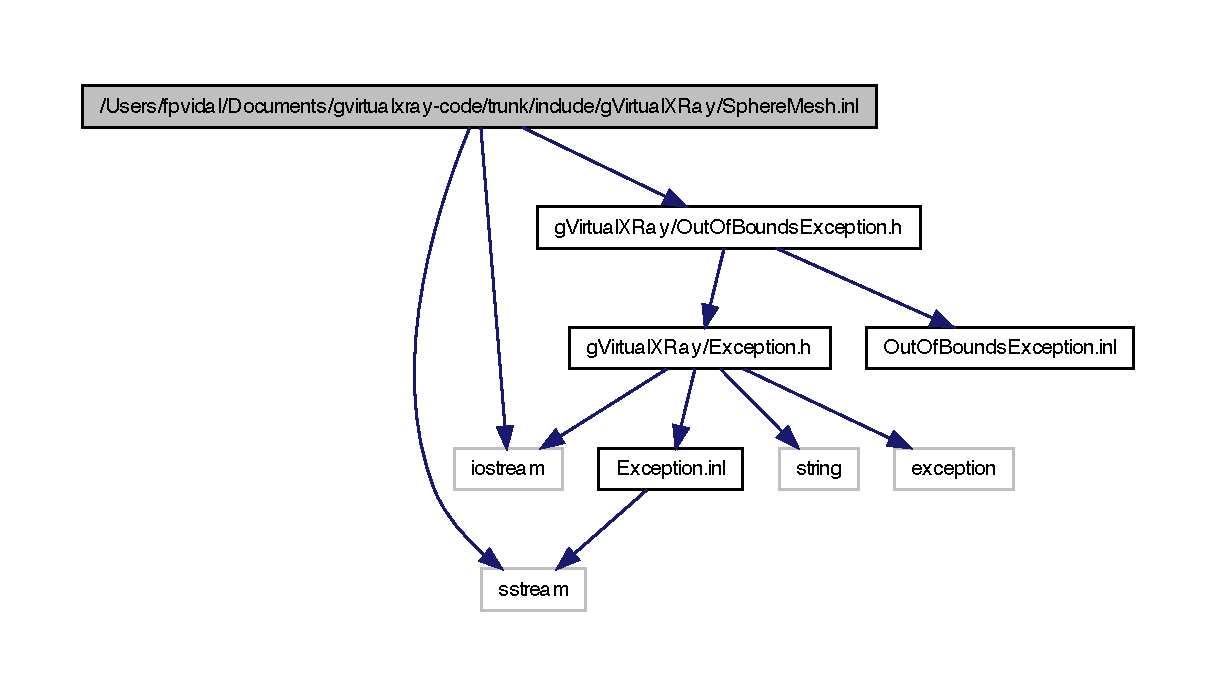
\includegraphics[width=400pt]{_sphere_mesh_8inl__incl}
\end{center}
\end{figure}
This graph shows which files directly or indirectly include this file:\nopagebreak
\begin{figure}[H]
\begin{center}
\leavevmode
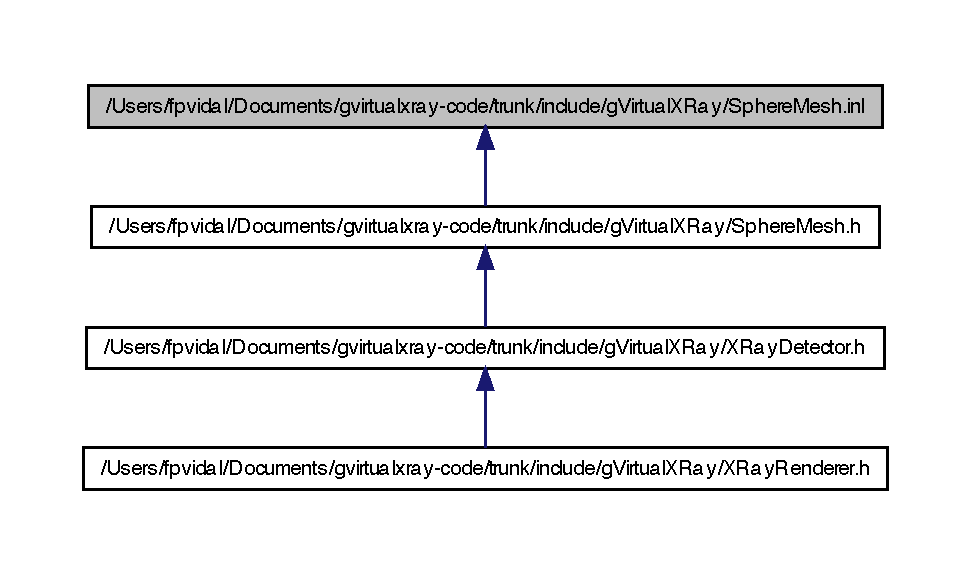
\includegraphics[width=400pt]{_sphere_mesh_8inl__dep__incl}
\end{center}
\end{figure}
\subsection*{Namespaces}
\begin{DoxyCompactItemize}
\item 
namespace \hyperlink{namespace_graphics}{Graphics}
\end{DoxyCompactItemize}


\subsection{Detailed Description}
Class to handle 3D meshes of spheres. \begin{DoxyVersion}{Version}
1.0
\end{DoxyVersion}
\begin{DoxyDate}{Date}
22/03/2014
\end{DoxyDate}
\begin{DoxyAuthor}{Author}
Dr Franck P. Vidal
\end{DoxyAuthor}
\begin{Desc}
\item[\hyperlink{todo__todo000005}{Todo}]Make it possible to merge vertices if an array of indices exists\end{Desc}
\hypertarget{_x_ray_renderer_8inl_License}{}\subsection{License}\label{_x_ray_renderer_8inl_License}
BSD 3-\/Clause License.

For details on use and redistribution please refer to \href{http://opensource.org/licenses/BSD-3-Clause}{\tt http://opensource.org/licenses/BSD-\/3-\/Clause}\hypertarget{_x_ray_renderer_8inl_Copyright}{}\subsection{Copyright}\label{_x_ray_renderer_8inl_Copyright}
(c) by Dr Franck P. Vidal (\href{mailto:franck.p.vidal@fpvidal.net}{\tt franck.p.vidal@fpvidal.net}), \href{http://www.fpvidal.net/,}{\tt http://www.fpvidal.net/,} Dec 2013, 2013, version 1.0, BSD 3-\/Clause License 

Definition in file \hyperlink{_sphere_mesh_8inl_source}{SphereMesh.inl}.


\hypertarget{_stereo_helper_8h}{
\section{/Users/fpvidal/Documents/gvirtualxray-\/code/trunk/include/gVirtualXRay/StereoHelper.h File Reference}
\label{_stereo_helper_8h}\index{/Users/fpvidal/Documents/gvirtualxray-\/code/trunk/include/gVirtualXRay/StereoHelper.h@{/Users/fpvidal/Documents/gvirtualxray-\/code/trunk/include/gVirtualXRay/StereoHelper.h}}
}


Class to handle stereo vision using OpenGL's quad buffer. The code is relying on // \href{http://www.orthostereo.com/geometryopengl.html.}{\tt http://www.orthostereo.com/geometryopengl.html.}  


{\ttfamily \#include \char`\"{}gVirtualXRay/Matrix4x4.h\char`\"{}}\par
{\ttfamily \#include \char`\"{}gVirtualXRay/Types.h\char`\"{}}\par
{\ttfamily \#include \char`\"{}StereoHelper.inl\char`\"{}}\par
Include dependency graph for StereoHelper.h:\nopagebreak
\begin{figure}[H]
\begin{center}
\leavevmode
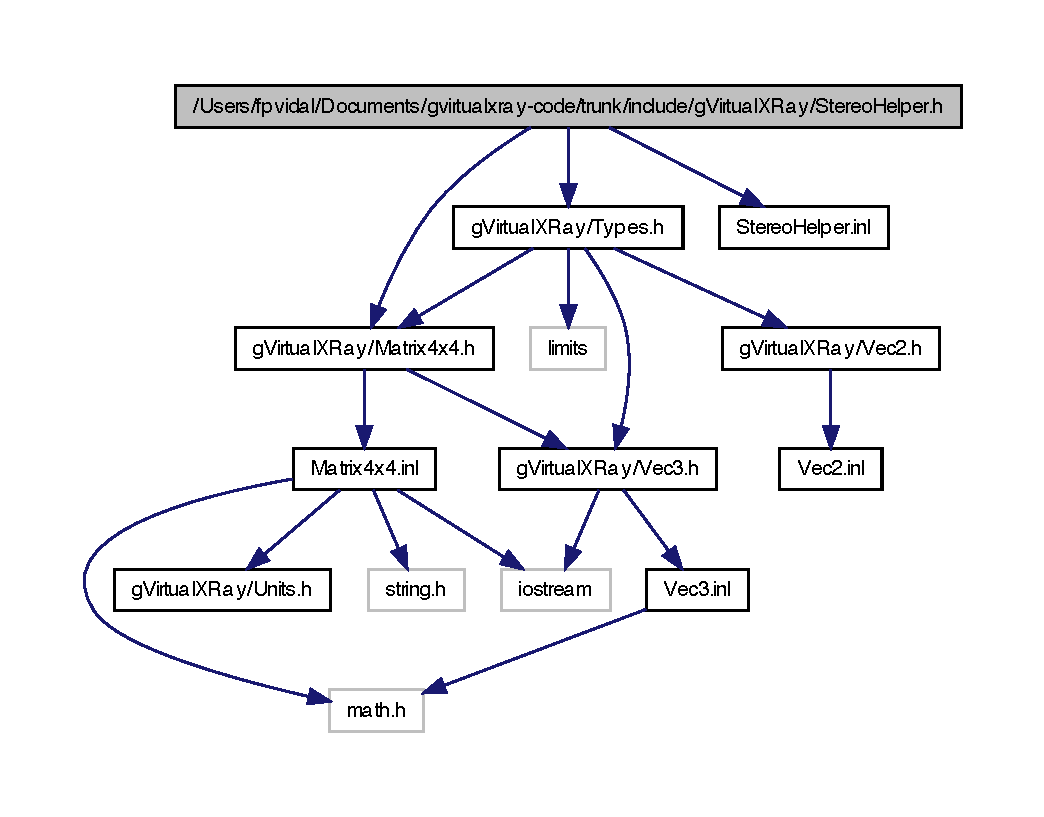
\includegraphics[width=400pt]{_stereo_helper_8h__incl}
\end{center}
\end{figure}
\subsection*{Classes}
\begin{DoxyCompactItemize}
\item 
class \hyperlink{class_graphics_1_1_stereo_helper}{Graphics::StereoHelper}
\begin{DoxyCompactList}\small\item\em \hyperlink{class_graphics_1_1_stereo_helper}{StereoHelper} is a class to handle stereo vision using OpenGL's quad buffer. \end{DoxyCompactList}\end{DoxyCompactItemize}
\subsection*{Namespaces}
\begin{DoxyCompactItemize}
\item 
namespace \hyperlink{namespace_graphics}{Graphics}
\end{DoxyCompactItemize}


\subsection{Detailed Description}
Class to handle stereo vision using OpenGL's quad buffer. The code is relying on // \href{http://www.orthostereo.com/geometryopengl.html.}{\tt http://www.orthostereo.com/geometryopengl.html.} \begin{DoxyVersion}{Version}
1.0
\end{DoxyVersion}
\begin{DoxyDate}{Date}
14/02/2014
\end{DoxyDate}
\begin{DoxyAuthor}{Author}
Dr Franck P. Vidal
\end{DoxyAuthor}
\hypertarget{_x_ray_renderer_8inl_License}{}\subsection{License}\label{_x_ray_renderer_8inl_License}
BSD 3-\/Clause License.

For details on use and redistribution please refer to \href{http://opensource.org/licenses/BSD-3-Clause}{\tt http://opensource.org/licenses/BSD-\/3-\/Clause}\hypertarget{_x_ray_renderer_8inl_Copyright}{}\subsection{Copyright}\label{_x_ray_renderer_8inl_Copyright}
(c) by Dr Franck P. Vidal (\href{mailto:franck.p.vidal@fpvidal.net}{\tt franck.p.vidal@fpvidal.net}), \href{http://www.fpvidal.net/,}{\tt http://www.fpvidal.net/,} Dec 2013, 2013, version 1.0, BSD 3-\/Clause License 

Definition in file \hyperlink{_stereo_helper_8h_source}{StereoHelper.h}.


\hypertarget{_stereo_helper_8inl}{
\section{/Users/fpvidal/Documents/gvirtualxray-\/code/trunk/include/gVirtualXRay/StereoHelper.inl File Reference}
\label{_stereo_helper_8inl}\index{/Users/fpvidal/Documents/gvirtualxray-\/code/trunk/include/gVirtualXRay/StereoHelper.inl@{/Users/fpvidal/Documents/gvirtualxray-\/code/trunk/include/gVirtualXRay/StereoHelper.inl}}
}


Class to handle stereo vision using OpenGL's quad buffer. The code is relying on // \href{http://www.orthostereo.com/geometryopengl.html.}{\tt http://www.orthostereo.com/geometryopengl.html.}  


This graph shows which files directly or indirectly include this file:\nopagebreak
\begin{figure}[H]
\begin{center}
\leavevmode
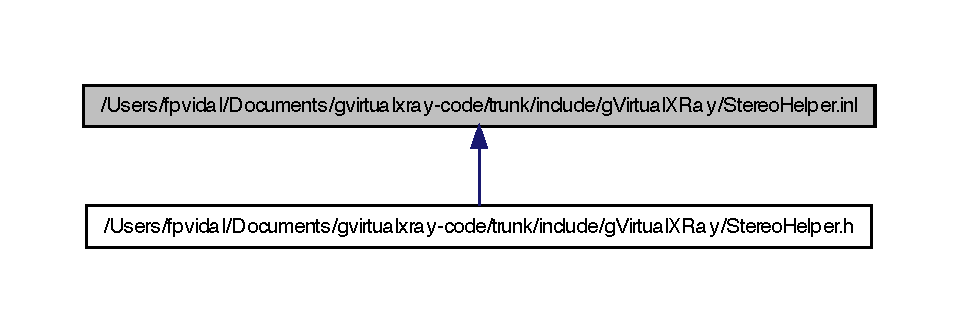
\includegraphics[width=400pt]{_stereo_helper_8inl__dep__incl}
\end{center}
\end{figure}
\subsection*{Namespaces}
\begin{DoxyCompactItemize}
\item 
namespace \hyperlink{namespace_graphics}{Graphics}
\end{DoxyCompactItemize}


\subsection{Detailed Description}
Class to handle stereo vision using OpenGL's quad buffer. The code is relying on // \href{http://www.orthostereo.com/geometryopengl.html.}{\tt http://www.orthostereo.com/geometryopengl.html.} \begin{DoxyVersion}{Version}
1.0
\end{DoxyVersion}
\begin{DoxyDate}{Date}
14/02/2014
\end{DoxyDate}
\begin{DoxyAuthor}{Author}
Dr Franck P. Vidal
\end{DoxyAuthor}
\hypertarget{_x_ray_renderer_8inl_License}{}\subsection{License}\label{_x_ray_renderer_8inl_License}
BSD 3-\/Clause License.

For details on use and redistribution please refer to \href{http://opensource.org/licenses/BSD-3-Clause}{\tt http://opensource.org/licenses/BSD-\/3-\/Clause}\hypertarget{_x_ray_renderer_8inl_Copyright}{}\subsection{Copyright}\label{_x_ray_renderer_8inl_Copyright}
(c) by Dr Franck P. Vidal (\href{mailto:franck.p.vidal@fpvidal.net}{\tt franck.p.vidal@fpvidal.net}), \href{http://www.fpvidal.net/,}{\tt http://www.fpvidal.net/,} Dec 2013, 2013, version 1.0, BSD 3-\/Clause License 

Definition in file \hyperlink{_stereo_helper_8inl_source}{StereoHelper.inl}.


\hypertarget{_types_8h}{
\section{/Users/fpvidal/Documents/gvirtualxray-\/code/trunk/include/gVirtualXRay/Types.h File Reference}
\label{_types_8h}\index{/Users/fpvidal/Documents/gvirtualxray-\/code/trunk/include/gVirtualXRay/Types.h@{/Users/fpvidal/Documents/gvirtualxray-\/code/trunk/include/gVirtualXRay/Types.h}}
}


Type declarations.  


{\ttfamily \#include $<$limits$>$}\par
{\ttfamily \#include \char`\"{}gVirtualXRay/Vec3.h\char`\"{}}\par
{\ttfamily \#include \char`\"{}gVirtualXRay/Vec2.h\char`\"{}}\par
{\ttfamily \#include \char`\"{}gVirtualXRay/Matrix4x4.h\char`\"{}}\par
Include dependency graph for Types.h:\nopagebreak
\begin{figure}[H]
\begin{center}
\leavevmode
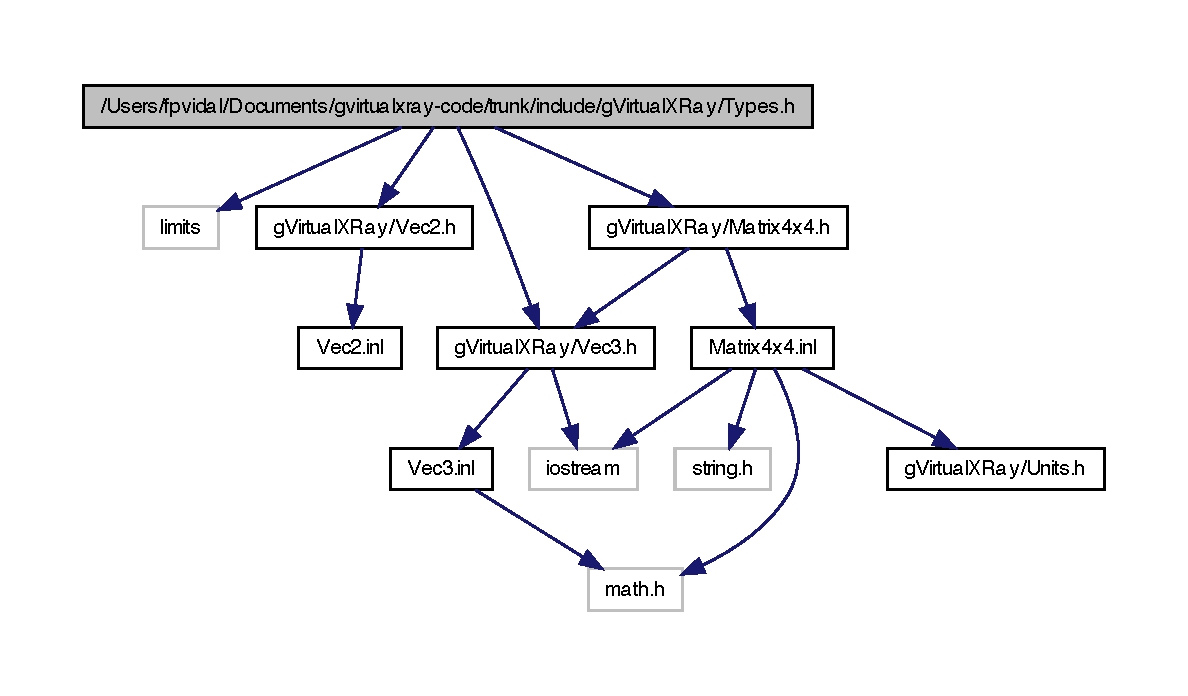
\includegraphics[width=400pt]{_types_8h__incl}
\end{center}
\end{figure}
This graph shows which files directly or indirectly include this file:
\nopagebreak
\begin{figure}[H]
\begin{center}
\leavevmode
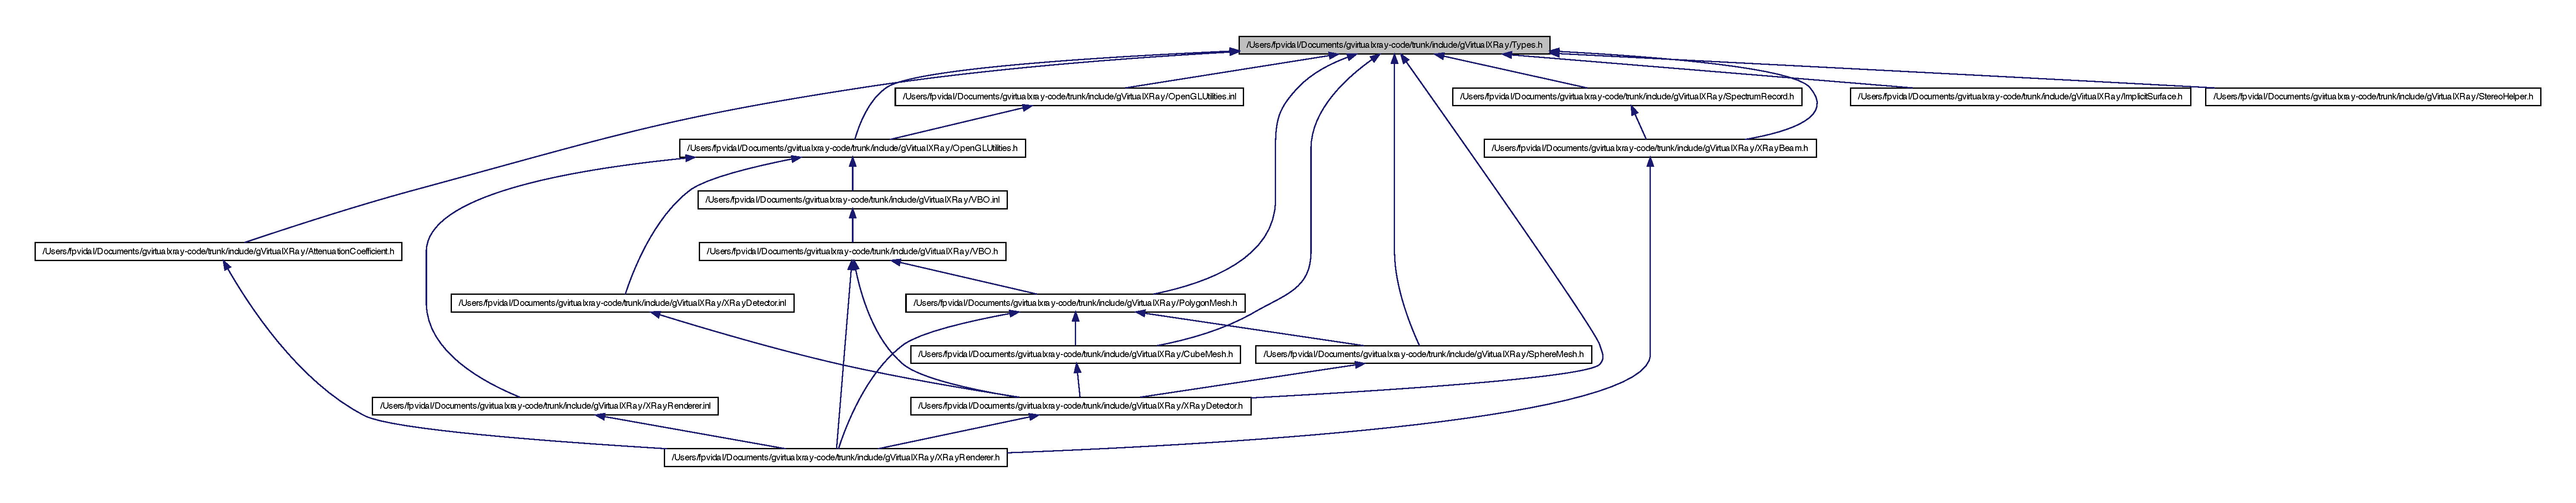
\includegraphics[width=400pt]{_types_8h__dep__incl}
\end{center}
\end{figure}
\subsection*{Namespaces}
\begin{DoxyCompactItemize}
\item 
namespace \hyperlink{namespace_utilities}{Utilities}
\end{DoxyCompactItemize}
\subsection*{Defines}
\begin{DoxyCompactItemize}
\item 
\#define \hyperlink{_types_8h_a253860d26dc1103520d36b81ac615da8}{RATIONAL\_\-NUMBER\_\-MAX}~FLT\_\-MAX
\begin{DoxyCompactList}\small\item\em Biggest value that can be stored with a real number. \end{DoxyCompactList}\item 
\#define \hyperlink{_types_8h_a002b2f4894492820fe708b1b7e7c5e70}{EPSILON}~0.0000001
\begin{DoxyCompactList}\small\item\em Smallest value that can be stored with a real number. \end{DoxyCompactList}\end{DoxyCompactItemize}
\subsection*{Typedefs}
\begin{DoxyCompactItemize}
\item 
typedef float \hyperlink{namespace_utilities_aec83622a80513f15f2bdee483a6af7a0}{Utilities::SinogramType}
\begin{DoxyCompactList}\small\item\em Type of data used to store sinograms. \end{DoxyCompactList}\item 
typedef float \hyperlink{namespace_utilities_a40969b96bd8d847b962e297cb79f08ce}{Utilities::RATIONAL\_\-NUMBER}
\begin{DoxyCompactList}\small\item\em Type of data used to store real numbers. \end{DoxyCompactList}\item 
typedef \hyperlink{class_math_1_1_vec2}{Vec2}$<$ RATIONAL\_\-NUMBER $>$ \hyperlink{namespace_utilities_a077a697d578c30ddec5ec97382be0a92}{Utilities::VEC2}
\begin{DoxyCompactList}\small\item\em Type of data used to store 2D vectors. \end{DoxyCompactList}\item 
typedef \hyperlink{class_math_1_1_vec3}{Vec3}$<$ RATIONAL\_\-NUMBER $>$ \hyperlink{namespace_utilities_af627ed108a4935196373499e157d3937}{Utilities::VEC3}
\begin{DoxyCompactList}\small\item\em Type of data used to store 3D vectors. \end{DoxyCompactList}\item 
typedef \hyperlink{class_math_1_1_matrix4x4}{Matrix4x4}$<$ RATIONAL\_\-NUMBER $>$ \hyperlink{namespace_utilities_a1e64fcb5d60661c7b2a3a5e7c96cc09f}{Utilities::MATRIX4}
\begin{DoxyCompactList}\small\item\em Type of data used to store 4x4 matrices. \end{DoxyCompactList}\item 
typedef \hyperlink{class_math_1_1_vec2}{Vec2}$<$ double $>$ \hyperlink{namespace_utilities_aaa021d29b05a070e411503f3a16dfcf7}{Utilities::Vec2d}
\begin{DoxyCompactList}\small\item\em Vec2d is a class to handle a 2D vector using double precision floating point numbers. \end{DoxyCompactList}\item 
typedef \hyperlink{class_math_1_1_vec2}{Vec2}$<$ float $>$ \hyperlink{namespace_utilities_ab79b80d506ad1b46bfb4f7979293d5d9}{Utilities::Vec2f}
\begin{DoxyCompactList}\small\item\em Vec2f is a class to handle a 2D vector using double precision floating point numbers. \end{DoxyCompactList}\item 
typedef \hyperlink{class_math_1_1_vec2}{Vec2}$<$ int $>$ \hyperlink{namespace_utilities_a491fc17b2e433b915d450c5fd8bcb459}{Utilities::Vec2i}
\begin{DoxyCompactList}\small\item\em Vec2i is a class to handle a 2D vector using 32 bits integers. \end{DoxyCompactList}\item 
typedef \hyperlink{class_math_1_1_vec2}{Vec2}$<$ unsigned int $>$ \hyperlink{namespace_utilities_a4a3a98a70cd4c9af9c3e49584516902f}{Utilities::Vec2ui}
\begin{DoxyCompactList}\small\item\em Vec2ui is a class to handle a 2D vector using unsigned 32 bits integers. \end{DoxyCompactList}\item 
typedef \hyperlink{class_math_1_1_vec3}{Vec3}$<$ double $>$ \hyperlink{namespace_utilities_ab28ebcaa8d9272ab9f9375205bded517}{Utilities::Vec3d}
\begin{DoxyCompactList}\small\item\em Vec3d is a class to handle a 3D vector using double precision floating point numbers. \end{DoxyCompactList}\item 
typedef \hyperlink{class_math_1_1_vec3}{Vec3}$<$ float $>$ \hyperlink{namespace_utilities_a39dfee93d59fd420ecf496f66606cbdd}{Utilities::Vec3f}
\begin{DoxyCompactList}\small\item\em Vec3f is a class to handle a 3D vector using double precision floating point numbers. \end{DoxyCompactList}\item 
typedef \hyperlink{class_math_1_1_vec3}{Vec3}$<$ int $>$ \hyperlink{namespace_utilities_a49caf0d054fbd5f9eb148ed40ad97dcc}{Utilities::Vec3i}
\begin{DoxyCompactList}\small\item\em Vec3i is a class to handle a 3D vector using signed 32 bits integers. \end{DoxyCompactList}\item 
typedef \hyperlink{class_math_1_1_vec3}{Vec3}$<$ unsigned int $>$ \hyperlink{namespace_utilities_ad931f5df25ecb686d1b3aea12bdc9d06}{Utilities::Vec3ui}
\begin{DoxyCompactList}\small\item\em Vec3ui is a class to handle a 3D vector using unsigned 32 bits integers. \end{DoxyCompactList}\item 
typedef \hyperlink{class_math_1_1_matrix4x4}{Matrix4x4}$<$ double $>$ \hyperlink{namespace_utilities_a1f0db90cea8d87567b4dd719ffd7d274}{Utilities::Matrix4x4d}
\begin{DoxyCompactList}\small\item\em Matrix4x4d is a class to handle a 4x4 matrix using double precision floating point numbers. \end{DoxyCompactList}\item 
typedef \hyperlink{class_math_1_1_matrix4x4}{Matrix4x4}$<$ float $>$ \hyperlink{namespace_utilities_a468a3c0ce8ea13f2b50bbc872a7a4bb7}{Utilities::Matrix4x4f}
\begin{DoxyCompactList}\small\item\em Matrix4x4f is a class to handle a 4x4 matrix using single precision floating point numbers. \end{DoxyCompactList}\end{DoxyCompactItemize}


\subsection{Detailed Description}
Type declarations. \begin{DoxyVersion}{Version}
1.0
\end{DoxyVersion}
\begin{DoxyDate}{Date}
08/11/2013
\end{DoxyDate}
\begin{DoxyAuthor}{Author}
Dr Franck P. Vidal
\end{DoxyAuthor}
\hypertarget{_x_ray_renderer_8inl_License}{}\subsection{License}\label{_x_ray_renderer_8inl_License}
BSD 3-\/Clause License.

For details on use and redistribution please refer to \href{http://opensource.org/licenses/BSD-3-Clause}{\tt http://opensource.org/licenses/BSD-\/3-\/Clause}\hypertarget{_x_ray_renderer_8inl_Copyright}{}\subsection{Copyright}\label{_x_ray_renderer_8inl_Copyright}
(c) by Dr Franck P. Vidal (\href{mailto:franck.p.vidal@fpvidal.net}{\tt franck.p.vidal@fpvidal.net}), \href{http://www.fpvidal.net/,}{\tt http://www.fpvidal.net/,} Dec 2013, 2013, version 1.0, BSD 3-\/Clause License 

Definition in file \hyperlink{_types_8h_source}{Types.h}.



\subsection{Define Documentation}
\hypertarget{_types_8h_a002b2f4894492820fe708b1b7e7c5e70}{
\index{Types.h@{Types.h}!EPSILON@{EPSILON}}
\index{EPSILON@{EPSILON}!Types.h@{Types.h}}
\subsubsection[{EPSILON}]{\setlength{\rightskip}{0pt plus 5cm}\#define EPSILON~0.0000001}}
\label{_types_8h_a002b2f4894492820fe708b1b7e7c5e70}


Smallest value that can be stored with a real number. 



Definition at line 71 of file Types.h.

\hypertarget{_types_8h_a253860d26dc1103520d36b81ac615da8}{
\index{Types.h@{Types.h}!RATIONAL\_\-NUMBER\_\-MAX@{RATIONAL\_\-NUMBER\_\-MAX}}
\index{RATIONAL\_\-NUMBER\_\-MAX@{RATIONAL\_\-NUMBER\_\-MAX}!Types.h@{Types.h}}
\subsubsection[{RATIONAL\_\-NUMBER\_\-MAX}]{\setlength{\rightskip}{0pt plus 5cm}\#define RATIONAL\_\-NUMBER\_\-MAX~FLT\_\-MAX}}
\label{_types_8h_a253860d26dc1103520d36b81ac615da8}


Biggest value that can be stored with a real number. 



Definition at line 67 of file Types.h.


\hypertarget{_units_8h}{
\section{/Users/fpvidal/Documents/gvirtualxray-\/code/trunk/include/gVirtualXRay/Units.h File Reference}
\label{_units_8h}\index{/Users/fpvidal/Documents/gvirtualxray-\/code/trunk/include/gVirtualXRay/Units.h@{/Users/fpvidal/Documents/gvirtualxray-\/code/trunk/include/gVirtualXRay/Units.h}}
}


Units, such as meters, etc.  


This graph shows which files directly or indirectly include this file:
\nopagebreak
\begin{figure}[H]
\begin{center}
\leavevmode
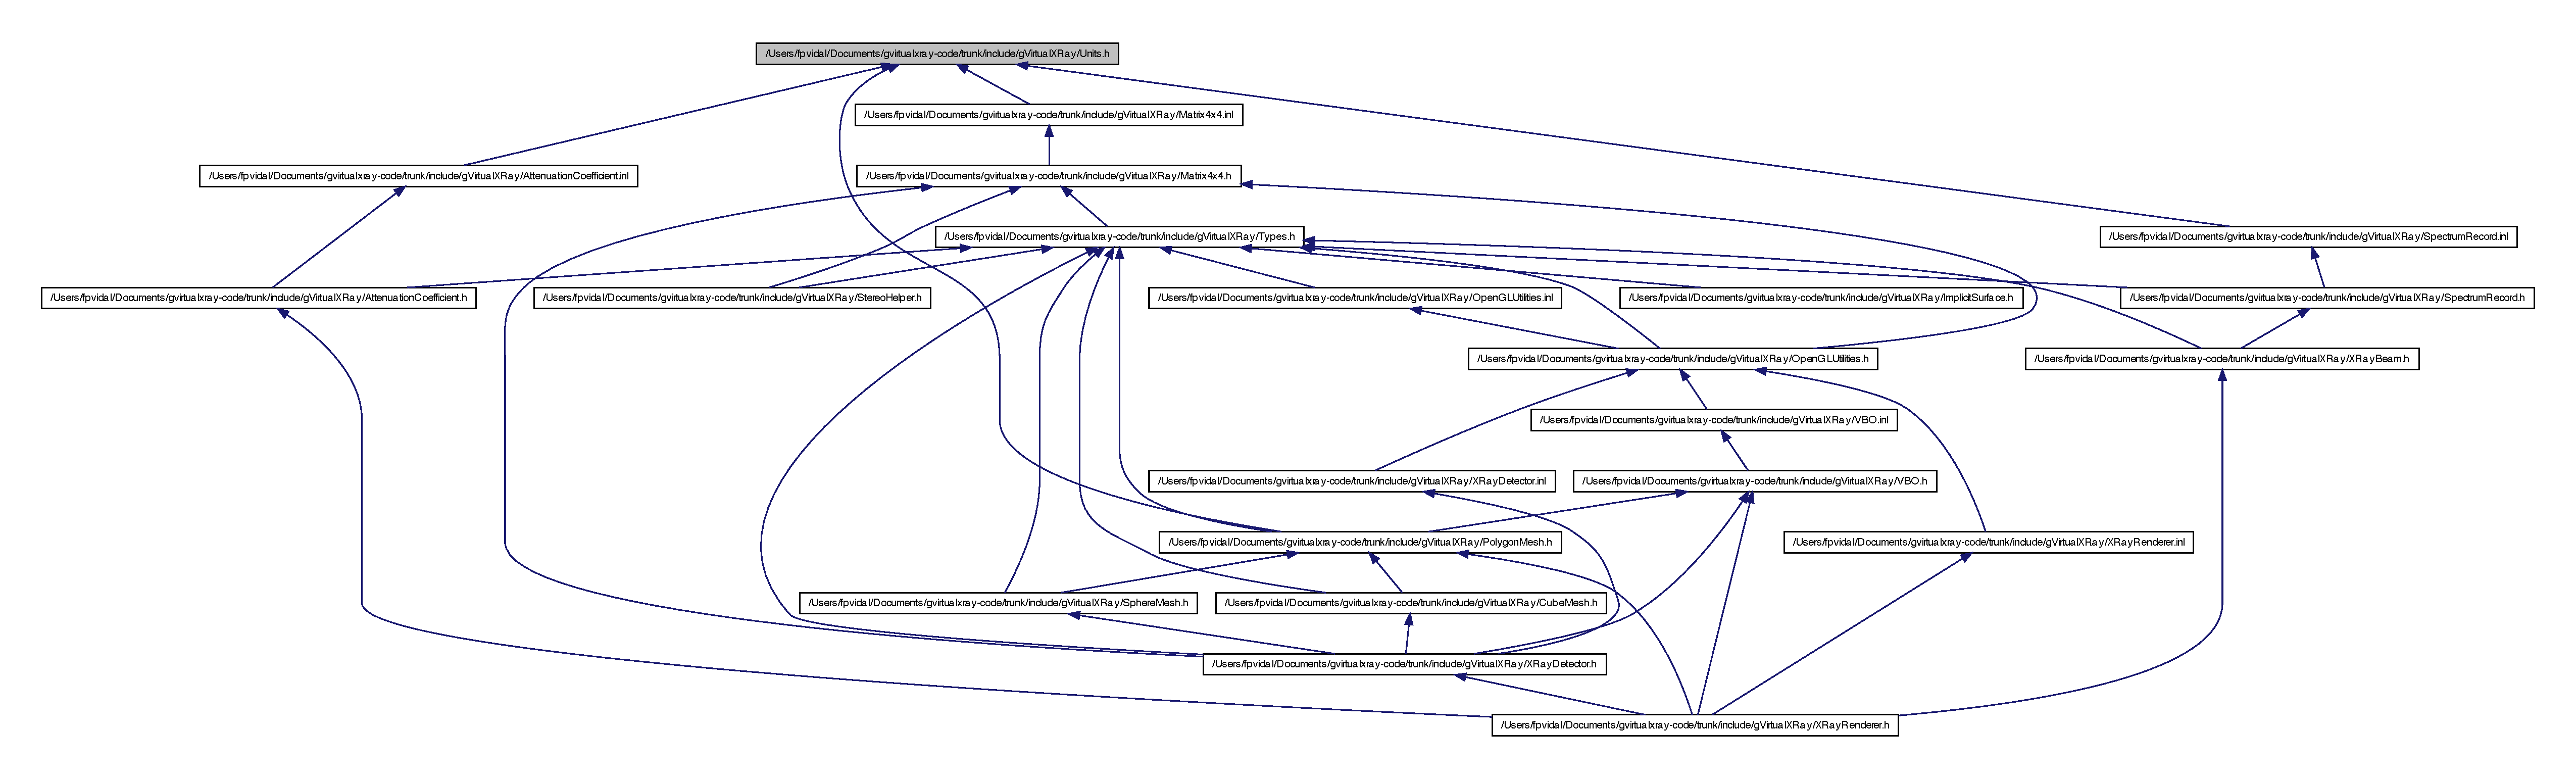
\includegraphics[width=400pt]{_units_8h__dep__incl}
\end{center}
\end{figure}
\subsection*{Namespaces}
\begin{DoxyCompactItemize}
\item 
namespace \hyperlink{namespace_utilities}{Utilities}
\end{DoxyCompactItemize}
\subsection*{Variables}
\begin{DoxyCompactItemize}
\item 
const double \hyperlink{namespace_utilities_a119d98992bec0bd0923f88ebf77ed86f}{Utilities::PI} = 3.14159265358979323846
\item 
const double \hyperlink{namespace_utilities_a3d5b18587a483b13232097d2ac93341f}{Utilities::PI\_\-2} = PI / 2.0
\item 
const double \hyperlink{namespace_utilities_a06654149ce3cba96084c785b079a7a31}{Utilities::kilometer} = 1000.0 / 0.001
\begin{DoxyCompactList}\small\item\em kilometre \end{DoxyCompactList}\item 
const double \hyperlink{namespace_utilities_a3fb2d462bd1e7dc8fe4dbc1ad4f28ff3}{Utilities::hectometer} = 100.0 / 0.001
\begin{DoxyCompactList}\small\item\em hectometre \end{DoxyCompactList}\item 
const double \hyperlink{namespace_utilities_a66e92dbad293594bf063d31aa9305983}{Utilities::decameter} = 10.0 / 0.001
\begin{DoxyCompactList}\small\item\em decametre \end{DoxyCompactList}\item 
const double \hyperlink{namespace_utilities_a2b626049c35729f994e12d5f4f950d6b}{Utilities::meter} = 1.0 / 0.001
\begin{DoxyCompactList}\small\item\em metre \end{DoxyCompactList}\item 
const double \hyperlink{namespace_utilities_a66145380051759756714059815f45e18}{Utilities::decimeter} = 0.1 / 0.001
\begin{DoxyCompactList}\small\item\em decimetre \end{DoxyCompactList}\item 
const double \hyperlink{namespace_utilities_a17483d8b3688f5a3786b48f4ed70588c}{Utilities::centimeter} = 0.01 / 0.001
\begin{DoxyCompactList}\small\item\em centimetre \end{DoxyCompactList}\item 
const double \hyperlink{namespace_utilities_ae8c7101098fba61f862817a083c422ca}{Utilities::millimeter} = 0.001 / 0.001
\begin{DoxyCompactList}\small\item\em millimetre \end{DoxyCompactList}\item 
const double \hyperlink{namespace_utilities_a99dfe40c94af0523293210aaf01a0435}{Utilities::micrometer} = 0.0001 / 0.001
\begin{DoxyCompactList}\small\item\em micrometre \end{DoxyCompactList}\item 
const double \hyperlink{namespace_utilities_ae059df9243c641262f7a72694479ab09}{Utilities::kilometre} = kilometer
\begin{DoxyCompactList}\small\item\em kilometre \end{DoxyCompactList}\item 
const double \hyperlink{namespace_utilities_ac838a64f1022b1f9cb88f0f641ee26b1}{Utilities::hectometre} = hectometer
\begin{DoxyCompactList}\small\item\em hectometre \end{DoxyCompactList}\item 
const double \hyperlink{namespace_utilities_ae6f96b1086168f4287845866c4a8a546}{Utilities::decametre} = decameter
\begin{DoxyCompactList}\small\item\em decametre \end{DoxyCompactList}\item 
const double \hyperlink{namespace_utilities_abf8ec967be8032f9546e417808f17cec}{Utilities::metre} = meter
\begin{DoxyCompactList}\small\item\em metre \end{DoxyCompactList}\item 
const double \hyperlink{namespace_utilities_acd1e513cc56efd8a5f237271a46afcfe}{Utilities::decimetre} = decimeter
\begin{DoxyCompactList}\small\item\em decimetre \end{DoxyCompactList}\item 
const double \hyperlink{namespace_utilities_a8f332608b463f7e22df3b1120be2cba2}{Utilities::centimetre} = centimeter
\begin{DoxyCompactList}\small\item\em centimetre \end{DoxyCompactList}\item 
const double \hyperlink{namespace_utilities_a8a754864202e3b90c9f70df567799d24}{Utilities::millimetre} = millimeter
\begin{DoxyCompactList}\small\item\em millimetre \end{DoxyCompactList}\item 
const double \hyperlink{namespace_utilities_a6d2f4eead5bcae530f7c08291bf86931}{Utilities::micrometre} = micrometer
\begin{DoxyCompactList}\small\item\em micrometre \end{DoxyCompactList}\item 
const double \hyperlink{namespace_utilities_a4e01876aaa4c4d98bcbf9526e980d996}{Utilities::km} = kilometer
\begin{DoxyCompactList}\small\item\em kilometre \end{DoxyCompactList}\item 
const double \hyperlink{namespace_utilities_aacdd5d6ef494c74b5292a3966a1bd5e7}{Utilities::hm} = hectometer
\begin{DoxyCompactList}\small\item\em hectometre \end{DoxyCompactList}\item 
const double \hyperlink{namespace_utilities_ad242ea541744880484ba811bc49fb881}{Utilities::dam} = decameter
\begin{DoxyCompactList}\small\item\em decametre \end{DoxyCompactList}\item 
const double \hyperlink{namespace_utilities_a205e9c8c24630292f2d0213f433503e9}{Utilities::m} = meter
\begin{DoxyCompactList}\small\item\em meter \end{DoxyCompactList}\item 
const double \hyperlink{namespace_utilities_a811d072b0676c0e47666a99c20fb5eee}{Utilities::dm} = decimeter
\begin{DoxyCompactList}\small\item\em decimeter \end{DoxyCompactList}\item 
const double \hyperlink{namespace_utilities_a43701408f4de13788368dce37066801f}{Utilities::cm} = centimeter
\begin{DoxyCompactList}\small\item\em centimeter \end{DoxyCompactList}\item 
const double \hyperlink{namespace_utilities_ada68d4ec8f02c2ffc43db9220cbdcba8}{Utilities::mm} = millimeter
\begin{DoxyCompactList}\small\item\em millimeter \end{DoxyCompactList}\item 
const double \hyperlink{namespace_utilities_a79bb1876d9d2416239e3ca0b57582018}{Utilities::um} = micrometer
\begin{DoxyCompactList}\small\item\em micrometre \end{DoxyCompactList}\item 
const double \hyperlink{namespace_utilities_a61a790dbfa282940ea38347f86885324}{Utilities::km2} = km $\ast$ km
\begin{DoxyCompactList}\small\item\em square kilometre \end{DoxyCompactList}\item 
const double \hyperlink{namespace_utilities_a437509ab345193dd1d6d41934f7ff284}{Utilities::hm2} = hm $\ast$ hm
\begin{DoxyCompactList}\small\item\em square hectometre \end{DoxyCompactList}\item 
const double \hyperlink{namespace_utilities_ab44794b92b08edcb68141cc381801bfc}{Utilities::dam2} = dam $\ast$ dam
\begin{DoxyCompactList}\small\item\em square decametre \end{DoxyCompactList}\item 
const double \hyperlink{namespace_utilities_aa5d500d1242875d68aabe2a7ca84dee6}{Utilities::m2} = m $\ast$ m
\begin{DoxyCompactList}\small\item\em square meter \end{DoxyCompactList}\item 
const double \hyperlink{namespace_utilities_a4221fcd40efde1b0ac518ca98c9b8371}{Utilities::dm2} = dm $\ast$ dm
\begin{DoxyCompactList}\small\item\em square decimeter \end{DoxyCompactList}\item 
const double \hyperlink{namespace_utilities_af8cd4e9cca8050523bb9ef0cc0519250}{Utilities::cm2} = cm $\ast$ cm
\begin{DoxyCompactList}\small\item\em square centimeter \end{DoxyCompactList}\item 
const double \hyperlink{namespace_utilities_a1bfe965c55c47b8f84c53b95d527da39}{Utilities::mm2} = mm $\ast$ mm
\begin{DoxyCompactList}\small\item\em square millimeter \end{DoxyCompactList}\item 
const double \hyperlink{namespace_utilities_a89e97d06d21d5752d28b987caca1164e}{Utilities::um2} = um $\ast$ um
\begin{DoxyCompactList}\small\item\em square micrometre \end{DoxyCompactList}\item 
const double \hyperlink{namespace_utilities_a9ae5f215b36e4775746428f61852bff9}{Utilities::megaelectronvolt} = 1.0
\begin{DoxyCompactList}\small\item\em megaelectron volt \end{DoxyCompactList}\item 
const double \hyperlink{namespace_utilities_adf9960a6afad6c0ee02c6a8104fe0bac}{Utilities::kiloelectronvolt} = megaelectronvolt $\ast$ 1.0e-\/3
\begin{DoxyCompactList}\small\item\em kiloelectron volt \end{DoxyCompactList}\item 
const double \hyperlink{namespace_utilities_a0045e627e65f14bccdf9ba29f46f4b39}{Utilities::electronvolt} = megaelectronvolt $\ast$ 1.0e-\/6
\begin{DoxyCompactList}\small\item\em electronvolt \end{DoxyCompactList}\item 
const double \hyperlink{namespace_utilities_a26374683c027fd82866b27124597f903}{Utilities::MeV} = megaelectronvolt
\begin{DoxyCompactList}\small\item\em megaelectron volt \end{DoxyCompactList}\item 
const double \hyperlink{namespace_utilities_a767ae2d5cc9d3f6e952a73c396d6a76b}{Utilities::keV} = kiloelectronvolt
\begin{DoxyCompactList}\small\item\em kiloelectron volt \end{DoxyCompactList}\item 
const double \hyperlink{namespace_utilities_a373e9baeec7c88baef6b6ba4f782097b}{Utilities::eV} = electronvolt
\begin{DoxyCompactList}\small\item\em electronvolt \end{DoxyCompactList}\item 
const double \hyperlink{namespace_utilities_a53892b9a331b44b7edb02383d2d3cc74}{Utilities::kilogram} = 1000.0
\begin{DoxyCompactList}\small\item\em kilogram \end{DoxyCompactList}\item 
const double \hyperlink{namespace_utilities_a06ccbbfaf687e7c9567fe53a74a815a4}{Utilities::hectogram} = 100.0
\begin{DoxyCompactList}\small\item\em hectogram \end{DoxyCompactList}\item 
const double \hyperlink{namespace_utilities_a0768cb48610ba03979360e95959f44d9}{Utilities::decagram} = 10.0
\begin{DoxyCompactList}\small\item\em decagram \end{DoxyCompactList}\item 
const double \hyperlink{namespace_utilities_a31f2c5ded8f5f13007b4704e0509ce8c}{Utilities::gram} = 1.0
\begin{DoxyCompactList}\small\item\em gram \end{DoxyCompactList}\item 
const double \hyperlink{namespace_utilities_a19cffac32ac7c8d1d469398620265431}{Utilities::decigram} = 0.1
\begin{DoxyCompactList}\small\item\em decigram \end{DoxyCompactList}\item 
const double \hyperlink{namespace_utilities_ae4b25dba2b30ec640f00b47acb80ff34}{Utilities::centigram} = 0.01
\begin{DoxyCompactList}\small\item\em centigram \end{DoxyCompactList}\item 
const double \hyperlink{namespace_utilities_acad791e8ae3f5eb81fa1aeb7abf90f9f}{Utilities::milligram} = 0.001
\begin{DoxyCompactList}\small\item\em milligram \end{DoxyCompactList}\item 
const double \hyperlink{namespace_utilities_ab9752f0a0b8174ed273a2a505c2a83e4}{Utilities::microgram} = 0.0001
\begin{DoxyCompactList}\small\item\em microgram \end{DoxyCompactList}\item 
const double \hyperlink{namespace_utilities_ade5640692129a688db6afa41d15d8778}{Utilities::kg} = kilogram
\begin{DoxyCompactList}\small\item\em kilogram \end{DoxyCompactList}\item 
const double \hyperlink{namespace_utilities_afce1fbb55c72d2f7670158b228e6be92}{Utilities::hg} = hectogram
\begin{DoxyCompactList}\small\item\em hectogram \end{DoxyCompactList}\item 
const double \hyperlink{namespace_utilities_a1a052c7a7614fc92834c71bc8029e0b3}{Utilities::dag} = decagram
\begin{DoxyCompactList}\small\item\em decagram \end{DoxyCompactList}\item 
const double \hyperlink{namespace_utilities_afa66a78e61dc36f0bf8236522c1d0495}{Utilities::g} = gram
\begin{DoxyCompactList}\small\item\em gram \end{DoxyCompactList}\item 
const double \hyperlink{namespace_utilities_a0560b0dea05b99f76fe3209784c11a14}{Utilities::dg} = decigram
\begin{DoxyCompactList}\small\item\em decigram \end{DoxyCompactList}\item 
const double \hyperlink{namespace_utilities_a8657e04ecc892b1e9a3b84db62bf94df}{Utilities::cg} = centigram
\begin{DoxyCompactList}\small\item\em centigram \end{DoxyCompactList}\item 
const double \hyperlink{namespace_utilities_a644a781a973f0febf71abf06c267c8f3}{Utilities::mg} = milligram
\begin{DoxyCompactList}\small\item\em milligram \end{DoxyCompactList}\item 
const double \hyperlink{namespace_utilities_ab7041baaaea73a172ddc834aaea10ec1}{Utilities::ug} = microgram
\begin{DoxyCompactList}\small\item\em microgram \end{DoxyCompactList}\end{DoxyCompactItemize}


\subsection{Detailed Description}
Units, such as meters, etc. \begin{DoxyVersion}{Version}
1.0
\end{DoxyVersion}
\begin{DoxyDate}{Date}
17/11/2013
\end{DoxyDate}
\begin{DoxyAuthor}{Author}
Dr Franck P. Vidal
\end{DoxyAuthor}
\hypertarget{_x_ray_renderer_8inl_License}{}\subsection{License}\label{_x_ray_renderer_8inl_License}
BSD 3-\/Clause License.

For details on use and redistribution please refer to \href{http://opensource.org/licenses/BSD-3-Clause}{\tt http://opensource.org/licenses/BSD-\/3-\/Clause}\hypertarget{_x_ray_renderer_8inl_Copyright}{}\subsection{Copyright}\label{_x_ray_renderer_8inl_Copyright}
(c) by Dr Franck P. Vidal (\href{mailto:franck.p.vidal@fpvidal.net}{\tt franck.p.vidal@fpvidal.net}), \href{http://www.fpvidal.net/,}{\tt http://www.fpvidal.net/,} Dec 2013, 2013, version 1.0, BSD 3-\/Clause License 

Definition in file \hyperlink{_units_8h_source}{Units.h}.


\hypertarget{_utilities_8h}{
\section{/Users/fpvidal/Documents/gvirtualxray-\/code/trunk/include/gVirtualXRay/Utilities.h File Reference}
\label{_utilities_8h}\index{/Users/fpvidal/Documents/gvirtualxray-\/code/trunk/include/gVirtualXRay/Utilities.h@{/Users/fpvidal/Documents/gvirtualxray-\/code/trunk/include/gVirtualXRay/Utilities.h}}
}


Some utility functions that do not fit anywhere else.  


\subsection*{Namespaces}
\begin{DoxyCompactItemize}
\item 
namespace \hyperlink{namespace_utilities}{Utilities}
\end{DoxyCompactItemize}
\subsection*{Functions}
\begin{DoxyCompactItemize}
\item 
int \hyperlink{namespace_utilities_aaa3b1ecb143bfae45b704d5a35bd8269}{Utilities::inflate} (const void $\ast$src, int srcLen, char $\ast$$\ast$apDst)
\begin{DoxyCompactList}\small\item\em Uncompress data using the Zlib. \end{DoxyCompactList}\end{DoxyCompactItemize}


\subsection{Detailed Description}
Some utility functions that do not fit anywhere else. \begin{DoxyVersion}{Version}
1.0
\end{DoxyVersion}
\begin{DoxyDate}{Date}
12/02/2014
\end{DoxyDate}
\begin{DoxyAuthor}{Author}
Dr Franck P. Vidal
\end{DoxyAuthor}
\hypertarget{_x_ray_renderer_8inl_License}{}\subsection{License}\label{_x_ray_renderer_8inl_License}
BSD 3-\/Clause License.

For details on use and redistribution please refer to \href{http://opensource.org/licenses/BSD-3-Clause}{\tt http://opensource.org/licenses/BSD-\/3-\/Clause}\hypertarget{_x_ray_renderer_8inl_Copyright}{}\subsection{Copyright}\label{_x_ray_renderer_8inl_Copyright}
(c) by Dr Franck P. Vidal (\href{mailto:franck.p.vidal@fpvidal.net}{\tt franck.p.vidal@fpvidal.net}), \href{http://www.fpvidal.net/,}{\tt http://www.fpvidal.net/,} Dec 2013, 2013, version 1.0, BSD 3-\/Clause License 

Definition in file \hyperlink{_utilities_8h_source}{Utilities.h}.


\hypertarget{_v_b_o_8h}{
\section{/Users/fpvidal/Documents/gvirtualxray-\/code/trunk/include/gVirtualXRay/VBO.h File Reference}
\label{_v_b_o_8h}\index{/Users/fpvidal/Documents/gvirtualxray-\/code/trunk/include/gVirtualXRay/VBO.h@{/Users/fpvidal/Documents/gvirtualxray-\/code/trunk/include/gVirtualXRay/VBO.h}}
}


Class to handle vertex buffer objects (VBOs).  


{\ttfamily \#include \char`\"{}VBO.inl\char`\"{}}\par
Include dependency graph for VBO.h:\nopagebreak
\begin{figure}[H]
\begin{center}
\leavevmode
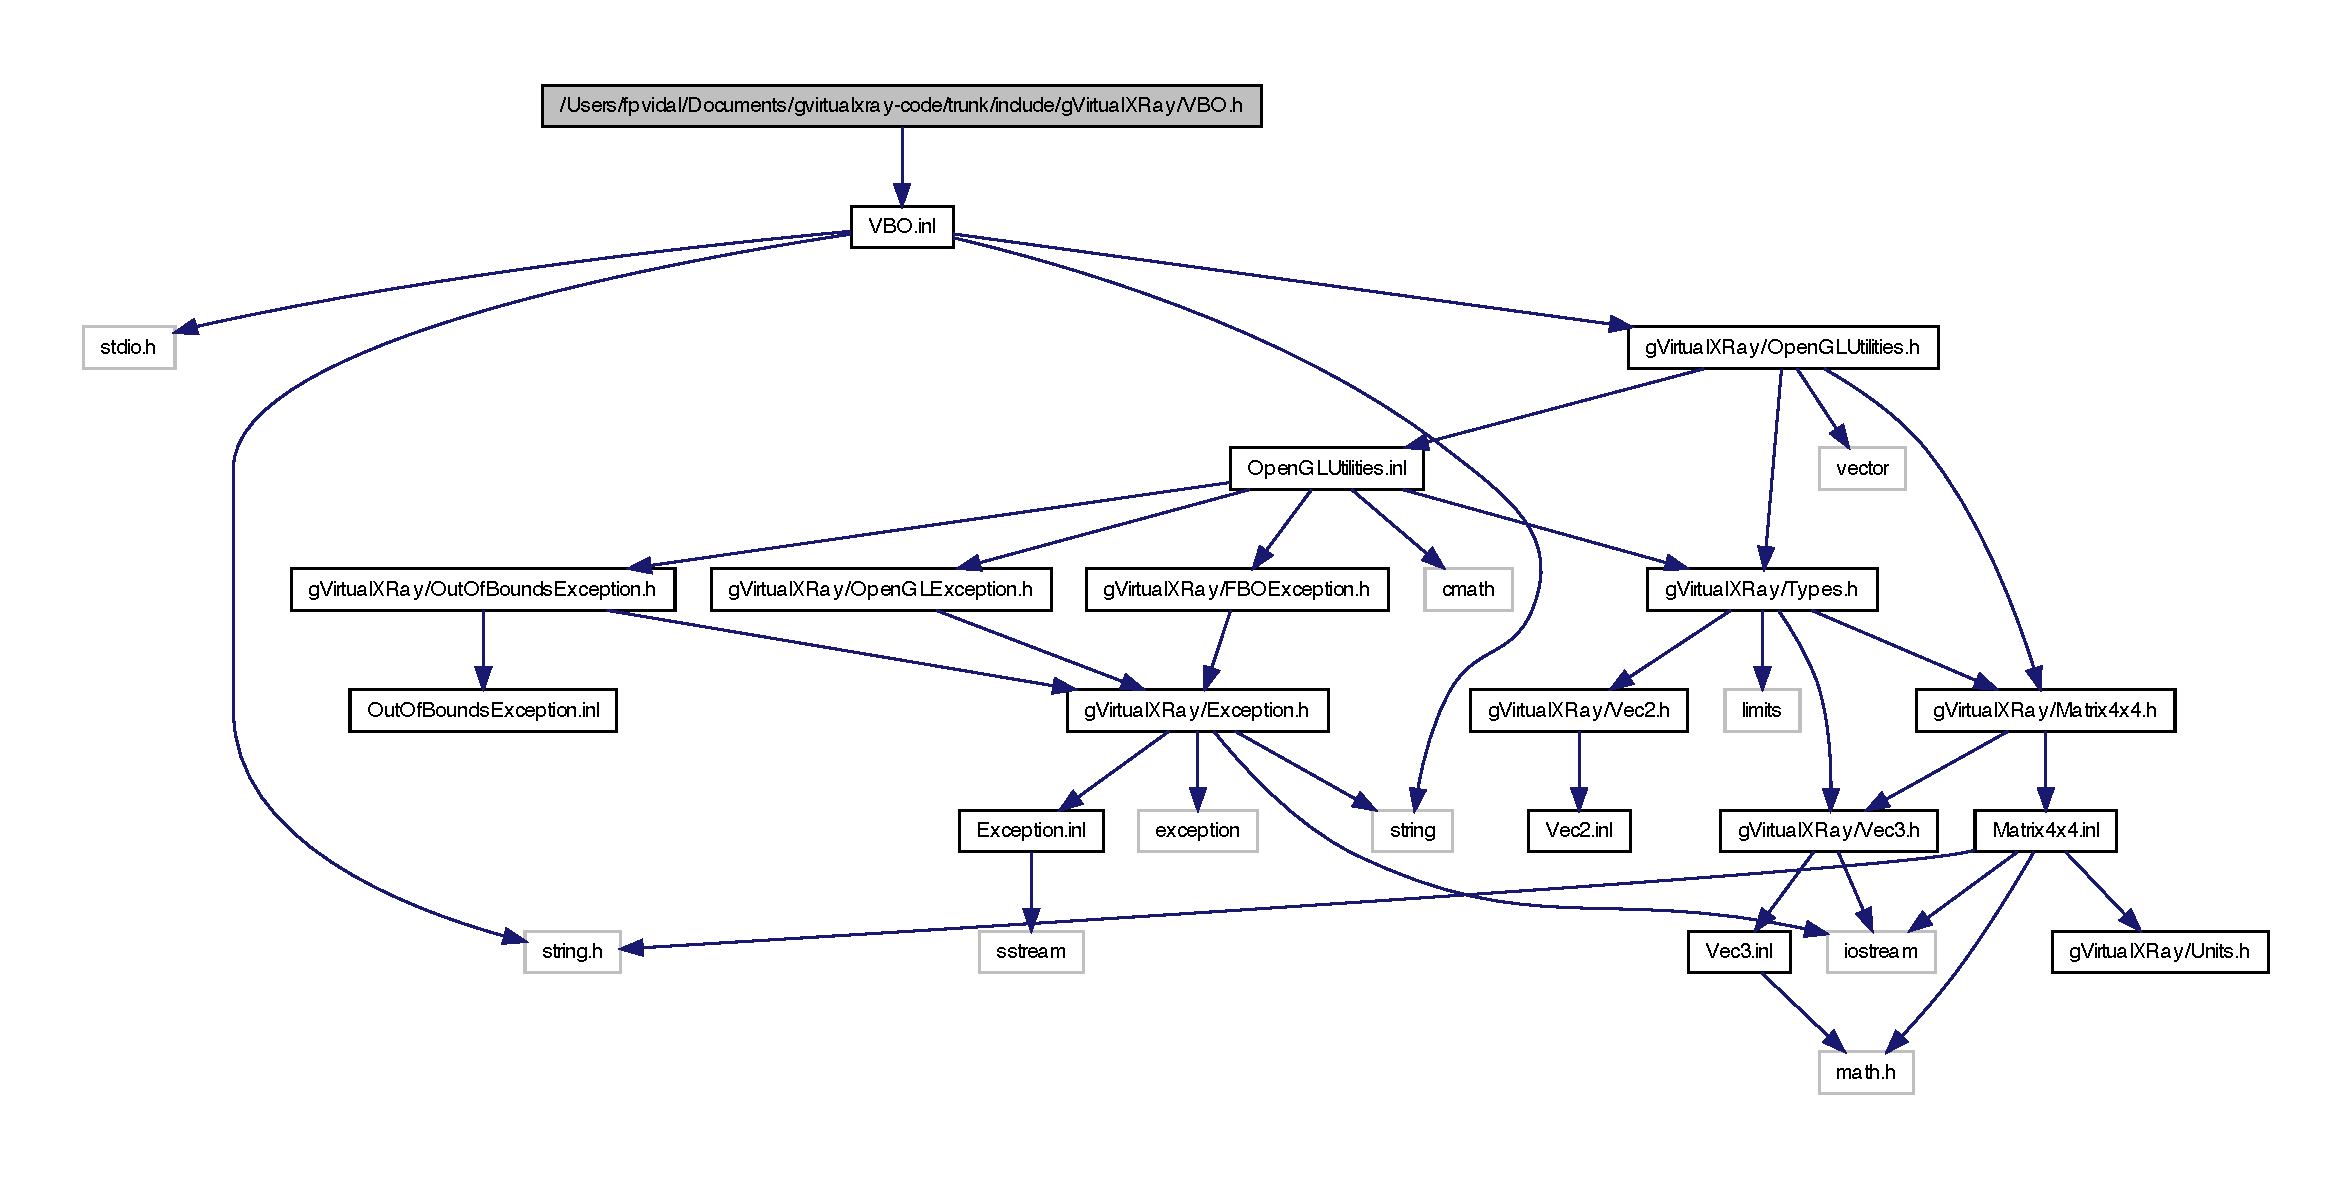
\includegraphics[width=400pt]{_v_b_o_8h__incl}
\end{center}
\end{figure}
This graph shows which files directly or indirectly include this file:
\nopagebreak
\begin{figure}[H]
\begin{center}
\leavevmode
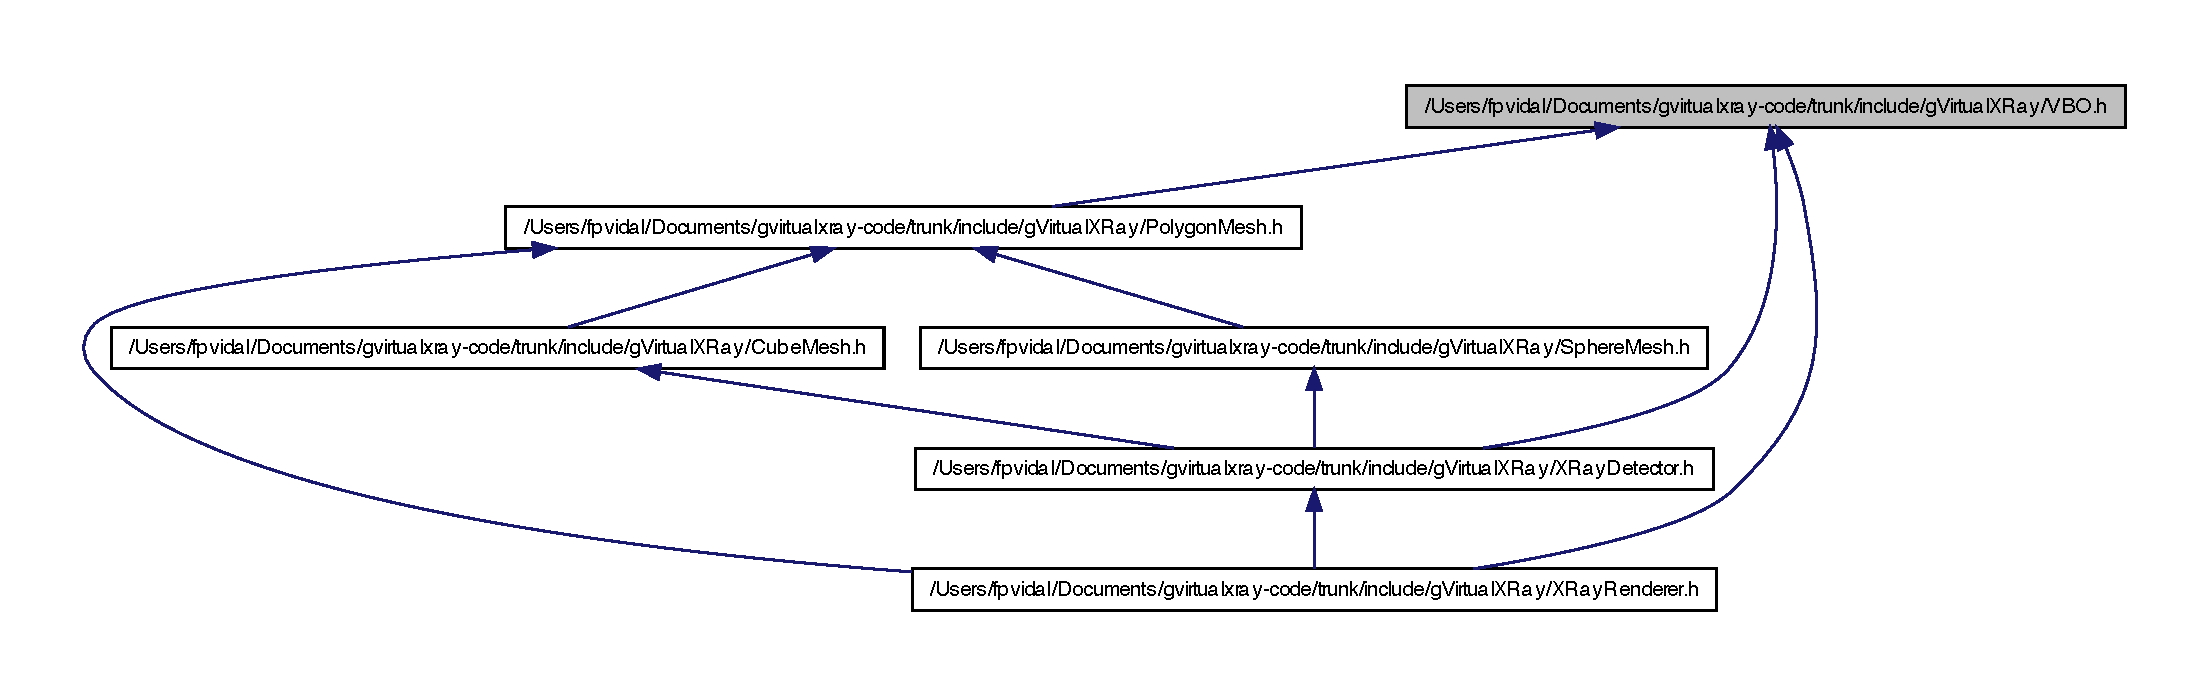
\includegraphics[width=400pt]{_v_b_o_8h__dep__incl}
\end{center}
\end{figure}
\subsection*{Classes}
\begin{DoxyCompactItemize}
\item 
class \hyperlink{class_graphics_1_1_v_b_o}{Graphics::VBO}
\begin{DoxyCompactList}\small\item\em \hyperlink{class_graphics_1_1_v_b_o}{VBO} is a class to handle a vertex buffer object (\hyperlink{class_graphics_1_1_v_b_o}{VBO}). \end{DoxyCompactList}\end{DoxyCompactItemize}
\subsection*{Namespaces}
\begin{DoxyCompactItemize}
\item 
namespace \hyperlink{namespace_graphics}{Graphics}
\end{DoxyCompactItemize}


\subsection{Detailed Description}
Class to handle vertex buffer objects (VBOs). \begin{DoxyVersion}{Version}
1.0
\end{DoxyVersion}
\begin{DoxyDate}{Date}
07/11/2013
\end{DoxyDate}
\begin{DoxyAuthor}{Author}
Dr Franck P. Vidal
\end{DoxyAuthor}
\hypertarget{_x_ray_renderer_8inl_License}{}\subsection{License}\label{_x_ray_renderer_8inl_License}
BSD 3-\/Clause License.

For details on use and redistribution please refer to \href{http://opensource.org/licenses/BSD-3-Clause}{\tt http://opensource.org/licenses/BSD-\/3-\/Clause}\hypertarget{_x_ray_renderer_8inl_Copyright}{}\subsection{Copyright}\label{_x_ray_renderer_8inl_Copyright}
(c) by Dr Franck P. Vidal (\href{mailto:franck.p.vidal@fpvidal.net}{\tt franck.p.vidal@fpvidal.net}), \href{http://www.fpvidal.net/,}{\tt http://www.fpvidal.net/,} Dec 2013, 2013, version 1.0, BSD 3-\/Clause License 

Definition in file \hyperlink{_v_b_o_8h_source}{VBO.h}.


\hypertarget{_v_b_o_8inl}{
\section{/Users/fpvidal/Documents/gvirtualxray-\/code/trunk/include/gVirtualXRay/VBO.inl File Reference}
\label{_v_b_o_8inl}\index{/Users/fpvidal/Documents/gvirtualxray-\/code/trunk/include/gVirtualXRay/VBO.inl@{/Users/fpvidal/Documents/gvirtualxray-\/code/trunk/include/gVirtualXRay/VBO.inl}}
}


Class to handle vertex buffer objects (VBOs).  


{\ttfamily \#include $<$stdio.h$>$}\par
{\ttfamily \#include $<$string$>$}\par
{\ttfamily \#include $<$string.h$>$}\par
{\ttfamily \#include \char`\"{}gVirtualXRay/OpenGLUtilities.h\char`\"{}}\par
Include dependency graph for VBO.inl:\nopagebreak
\begin{figure}[H]
\begin{center}
\leavevmode
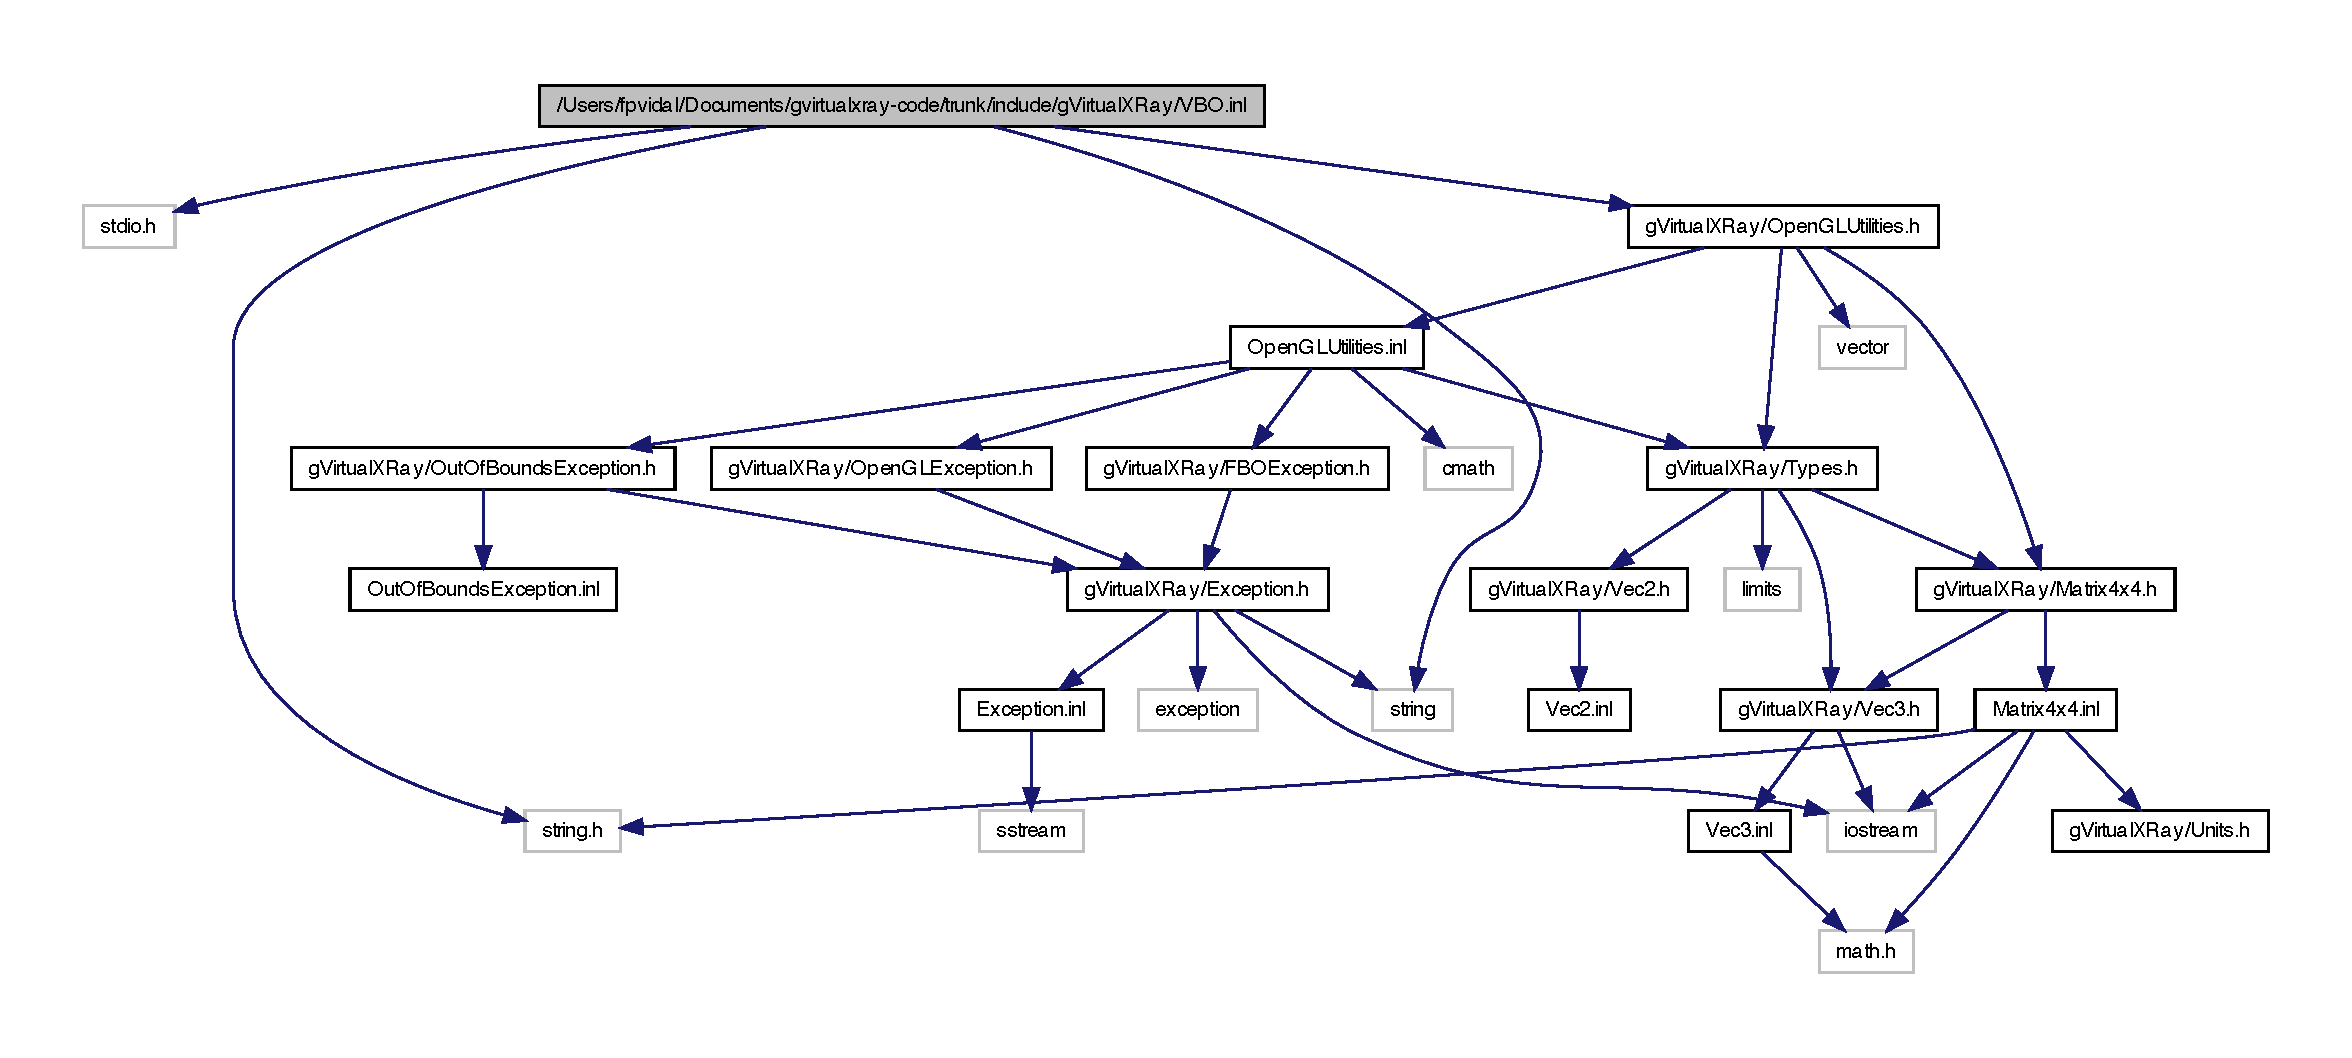
\includegraphics[width=400pt]{_v_b_o_8inl__incl}
\end{center}
\end{figure}
This graph shows which files directly or indirectly include this file:
\nopagebreak
\begin{figure}[H]
\begin{center}
\leavevmode
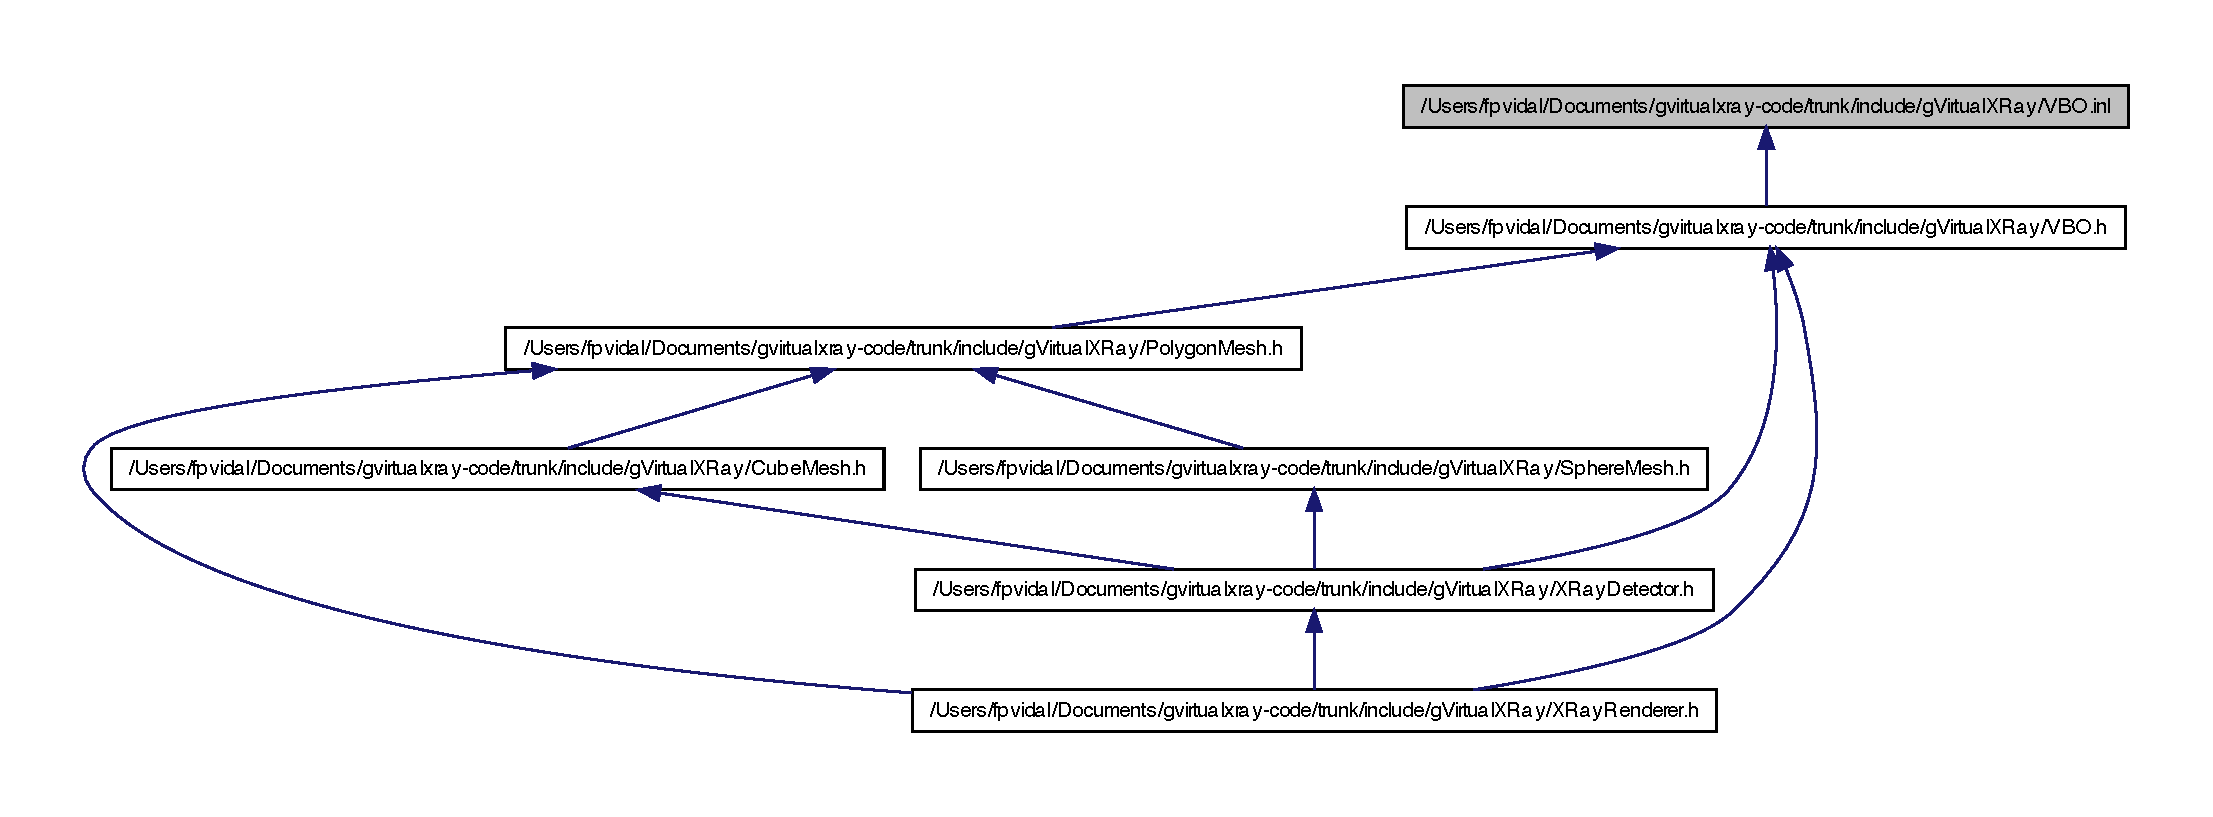
\includegraphics[width=400pt]{_v_b_o_8inl__dep__incl}
\end{center}
\end{figure}
\subsection*{Namespaces}
\begin{DoxyCompactItemize}
\item 
namespace \hyperlink{namespace_graphics}{Graphics}
\end{DoxyCompactItemize}
\subsection*{Defines}
\begin{DoxyCompactItemize}
\item 
\#define \hyperlink{_v_b_o_8inl_a3166a9728b4bb994b2efa80375301e81}{VBO\_\-BUFFER\_\-OFFSET}(a)~((char$\ast$)NULL + (a))
\item 
\#define \hyperlink{_v_b_o_8inl_a51866ad5778631c316d6cf5ac0d72396}{VERTEX\_\-SET\_\-ID}~0
\item 
\#define \hyperlink{_v_b_o_8inl_ac981e1349645a7ca16ba9b1a674783d5}{TEXT\_\-COORD\_\-SET\_\-ID}~1
\item 
\#define \hyperlink{_v_b_o_8inl_a9ba486f297d904dd1558d225e64923ed}{NORMAL\_\-SET\_\-ID}~2
\item 
\#define \hyperlink{_v_b_o_8inl_a3abfde2238b90851090b81855ff71070}{INDEX\_\-SET\_\-ID}~3
\end{DoxyCompactItemize}


\subsection{Detailed Description}
Class to handle vertex buffer objects (VBOs). \begin{DoxyVersion}{Version}
1.0
\end{DoxyVersion}
\begin{DoxyDate}{Date}
07/11/2013
\end{DoxyDate}
\begin{DoxyAuthor}{Author}
Dr Franck P. Vidal
\end{DoxyAuthor}
\hypertarget{_x_ray_renderer_8inl_License}{}\subsection{License}\label{_x_ray_renderer_8inl_License}
BSD 3-\/Clause License.

For details on use and redistribution please refer to \href{http://opensource.org/licenses/BSD-3-Clause}{\tt http://opensource.org/licenses/BSD-\/3-\/Clause}\hypertarget{_x_ray_renderer_8inl_Copyright}{}\subsection{Copyright}\label{_x_ray_renderer_8inl_Copyright}
(c) by Dr Franck P. Vidal (\href{mailto:franck.p.vidal@fpvidal.net}{\tt franck.p.vidal@fpvidal.net}), \href{http://www.fpvidal.net/,}{\tt http://www.fpvidal.net/,} Dec 2013, 2013, version 1.0, BSD 3-\/Clause License 

Definition in file \hyperlink{_v_b_o_8inl_source}{VBO.inl}.



\subsection{Define Documentation}
\hypertarget{_v_b_o_8inl_a3abfde2238b90851090b81855ff71070}{
\index{VBO.inl@{VBO.inl}!INDEX\_\-SET\_\-ID@{INDEX\_\-SET\_\-ID}}
\index{INDEX\_\-SET\_\-ID@{INDEX\_\-SET\_\-ID}!VBO.inl@{VBO.inl}}
\subsubsection[{INDEX\_\-SET\_\-ID}]{\setlength{\rightskip}{0pt plus 5cm}\#define INDEX\_\-SET\_\-ID~3}}
\label{_v_b_o_8inl_a3abfde2238b90851090b81855ff71070}


Definition at line 48 of file VBO.inl.

\hypertarget{_v_b_o_8inl_a9ba486f297d904dd1558d225e64923ed}{
\index{VBO.inl@{VBO.inl}!NORMAL\_\-SET\_\-ID@{NORMAL\_\-SET\_\-ID}}
\index{NORMAL\_\-SET\_\-ID@{NORMAL\_\-SET\_\-ID}!VBO.inl@{VBO.inl}}
\subsubsection[{NORMAL\_\-SET\_\-ID}]{\setlength{\rightskip}{0pt plus 5cm}\#define NORMAL\_\-SET\_\-ID~2}}
\label{_v_b_o_8inl_a9ba486f297d904dd1558d225e64923ed}


Definition at line 47 of file VBO.inl.

\hypertarget{_v_b_o_8inl_ac981e1349645a7ca16ba9b1a674783d5}{
\index{VBO.inl@{VBO.inl}!TEXT\_\-COORD\_\-SET\_\-ID@{TEXT\_\-COORD\_\-SET\_\-ID}}
\index{TEXT\_\-COORD\_\-SET\_\-ID@{TEXT\_\-COORD\_\-SET\_\-ID}!VBO.inl@{VBO.inl}}
\subsubsection[{TEXT\_\-COORD\_\-SET\_\-ID}]{\setlength{\rightskip}{0pt plus 5cm}\#define TEXT\_\-COORD\_\-SET\_\-ID~1}}
\label{_v_b_o_8inl_ac981e1349645a7ca16ba9b1a674783d5}


Definition at line 46 of file VBO.inl.

\hypertarget{_v_b_o_8inl_a3166a9728b4bb994b2efa80375301e81}{
\index{VBO.inl@{VBO.inl}!VBO\_\-BUFFER\_\-OFFSET@{VBO\_\-BUFFER\_\-OFFSET}}
\index{VBO\_\-BUFFER\_\-OFFSET@{VBO\_\-BUFFER\_\-OFFSET}!VBO.inl@{VBO.inl}}
\subsubsection[{VBO\_\-BUFFER\_\-OFFSET}]{\setlength{\rightskip}{0pt plus 5cm}\#define VBO\_\-BUFFER\_\-OFFSET(
\begin{DoxyParamCaption}
\item[{}]{a}
\end{DoxyParamCaption}
)~((char$\ast$)NULL + (a))}}
\label{_v_b_o_8inl_a3166a9728b4bb994b2efa80375301e81}


Definition at line 44 of file VBO.inl.

\hypertarget{_v_b_o_8inl_a51866ad5778631c316d6cf5ac0d72396}{
\index{VBO.inl@{VBO.inl}!VERTEX\_\-SET\_\-ID@{VERTEX\_\-SET\_\-ID}}
\index{VERTEX\_\-SET\_\-ID@{VERTEX\_\-SET\_\-ID}!VBO.inl@{VBO.inl}}
\subsubsection[{VERTEX\_\-SET\_\-ID}]{\setlength{\rightskip}{0pt plus 5cm}\#define VERTEX\_\-SET\_\-ID~0}}
\label{_v_b_o_8inl_a51866ad5778631c316d6cf5ac0d72396}


Definition at line 45 of file VBO.inl.


\hypertarget{_vec2_8h}{
\section{/Users/fpvidal/Documents/gvirtualxray-\/code/trunk/include/gVirtualXRay/Vec2.h File Reference}
\label{_vec2_8h}\index{/Users/fpvidal/Documents/gvirtualxray-\/code/trunk/include/gVirtualXRay/Vec2.h@{/Users/fpvidal/Documents/gvirtualxray-\/code/trunk/include/gVirtualXRay/Vec2.h}}
}


Template class to handle 2D vectors.  


{\ttfamily \#include \char`\"{}Vec2.inl\char`\"{}}\par
Include dependency graph for Vec2.h:\nopagebreak
\begin{figure}[H]
\begin{center}
\leavevmode
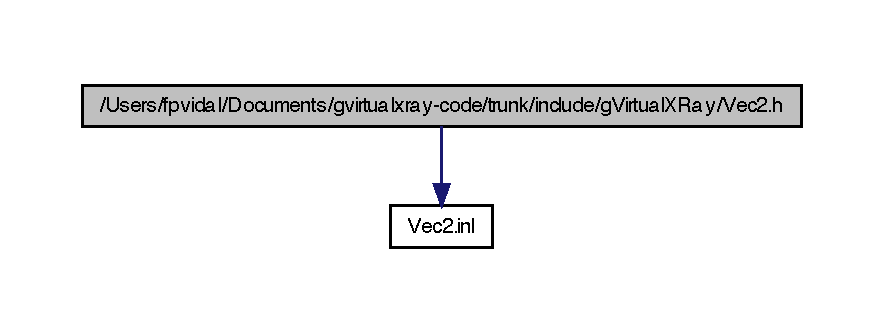
\includegraphics[width=400pt]{_vec2_8h__incl}
\end{center}
\end{figure}
This graph shows which files directly or indirectly include this file:
\nopagebreak
\begin{figure}[H]
\begin{center}
\leavevmode
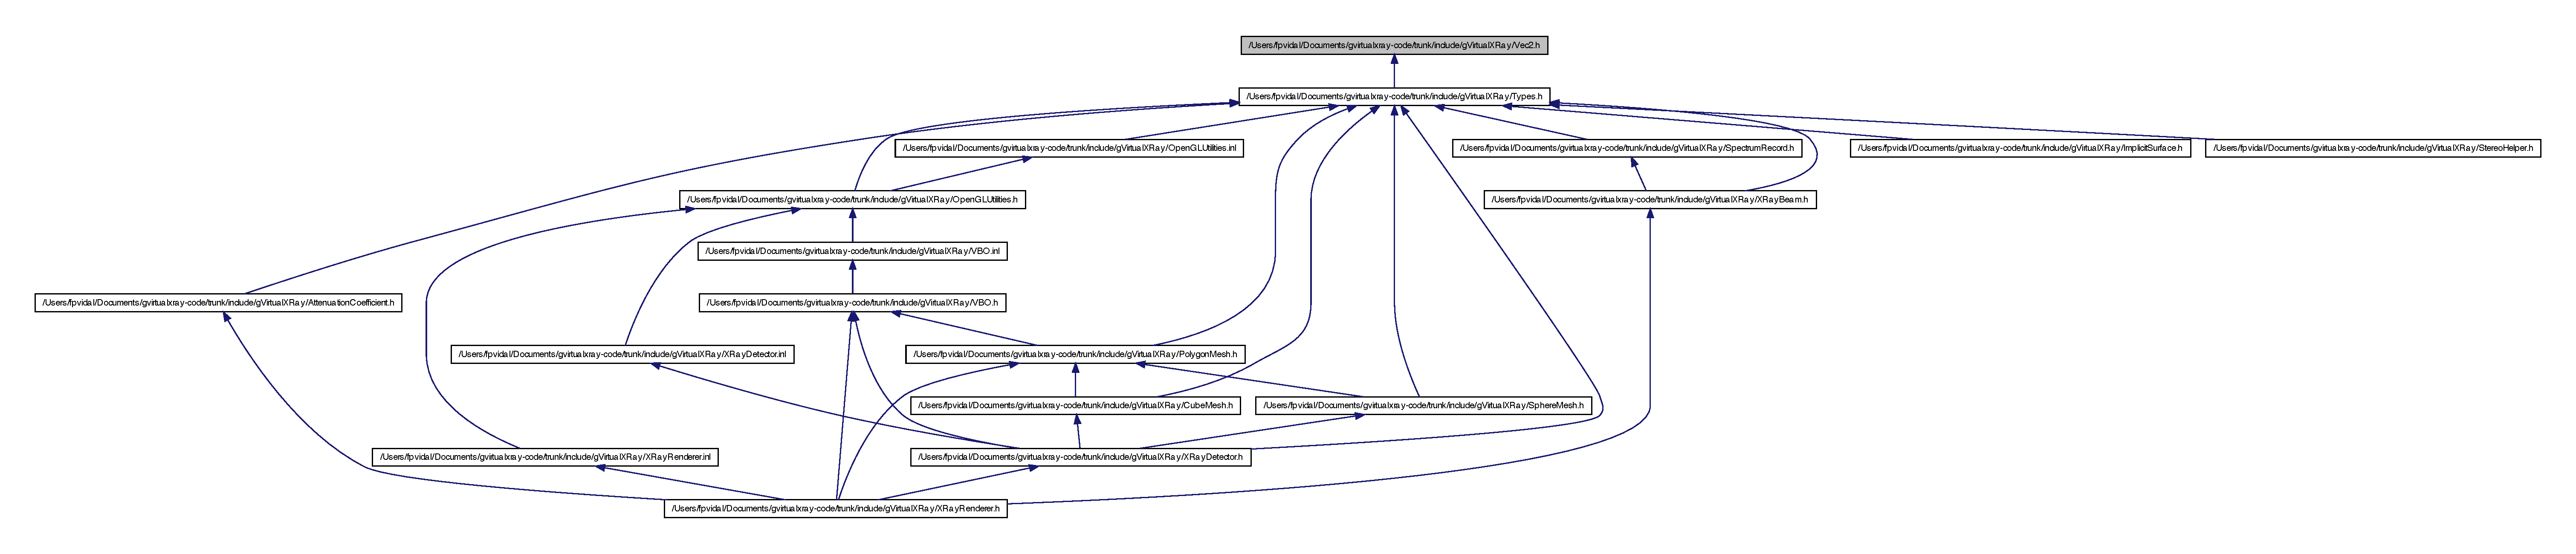
\includegraphics[width=400pt]{_vec2_8h__dep__incl}
\end{center}
\end{figure}
\subsection*{Classes}
\begin{DoxyCompactItemize}
\item 
class \hyperlink{class_math_1_1_vec2}{Math::Vec2$<$ T $>$}
\begin{DoxyCompactList}\small\item\em \hyperlink{class_math_1_1_vec2}{Vec2} is a template class to handle a 2D vector. \end{DoxyCompactList}\end{DoxyCompactItemize}
\subsection*{Namespaces}
\begin{DoxyCompactItemize}
\item 
namespace \hyperlink{namespace_math}{Math}
\end{DoxyCompactItemize}
\subsection*{Functions}
\begin{DoxyCompactItemize}
\item 
{\footnotesize template$<$typename T $>$ }\\std::ostream \& \hyperlink{namespace_math_ae50cf02c21b5ac0d5823b4c241a78e4a}{Math::operator$<$$<$} (std::ostream \&anOutputStream, const Vec2$<$ T $>$ \&aVector)
\end{DoxyCompactItemize}


\subsection{Detailed Description}
Template class to handle 2D vectors. \begin{DoxyVersion}{Version}
1.0
\end{DoxyVersion}
\begin{DoxyDate}{Date}
11/11/2013
\end{DoxyDate}
\begin{DoxyAuthor}{Author}
Dr Franck P. Vidal
\end{DoxyAuthor}
\hypertarget{_x_ray_renderer_8inl_License}{}\subsection{License}\label{_x_ray_renderer_8inl_License}
BSD 3-\/Clause License.

For details on use and redistribution please refer to \href{http://opensource.org/licenses/BSD-3-Clause}{\tt http://opensource.org/licenses/BSD-\/3-\/Clause}\hypertarget{_x_ray_renderer_8inl_Copyright}{}\subsection{Copyright}\label{_x_ray_renderer_8inl_Copyright}
(c) by Dr Franck P. Vidal (\href{mailto:franck.p.vidal@fpvidal.net}{\tt franck.p.vidal@fpvidal.net}), \href{http://www.fpvidal.net/,}{\tt http://www.fpvidal.net/,} Dec 2013, 2013, version 1.0, BSD 3-\/Clause License 

Definition in file \hyperlink{_vec2_8h_source}{Vec2.h}.


\hypertarget{_vec2_8inl}{
\section{/Users/fpvidal/Documents/gvirtualxray-\/code/trunk/include/gVirtualXRay/Vec2.inl File Reference}
\label{_vec2_8inl}\index{/Users/fpvidal/Documents/gvirtualxray-\/code/trunk/include/gVirtualXRay/Vec2.inl@{/Users/fpvidal/Documents/gvirtualxray-\/code/trunk/include/gVirtualXRay/Vec2.inl}}
}


Template class to handle 2D vectors.  


This graph shows which files directly or indirectly include this file:
\nopagebreak
\begin{figure}[H]
\begin{center}
\leavevmode
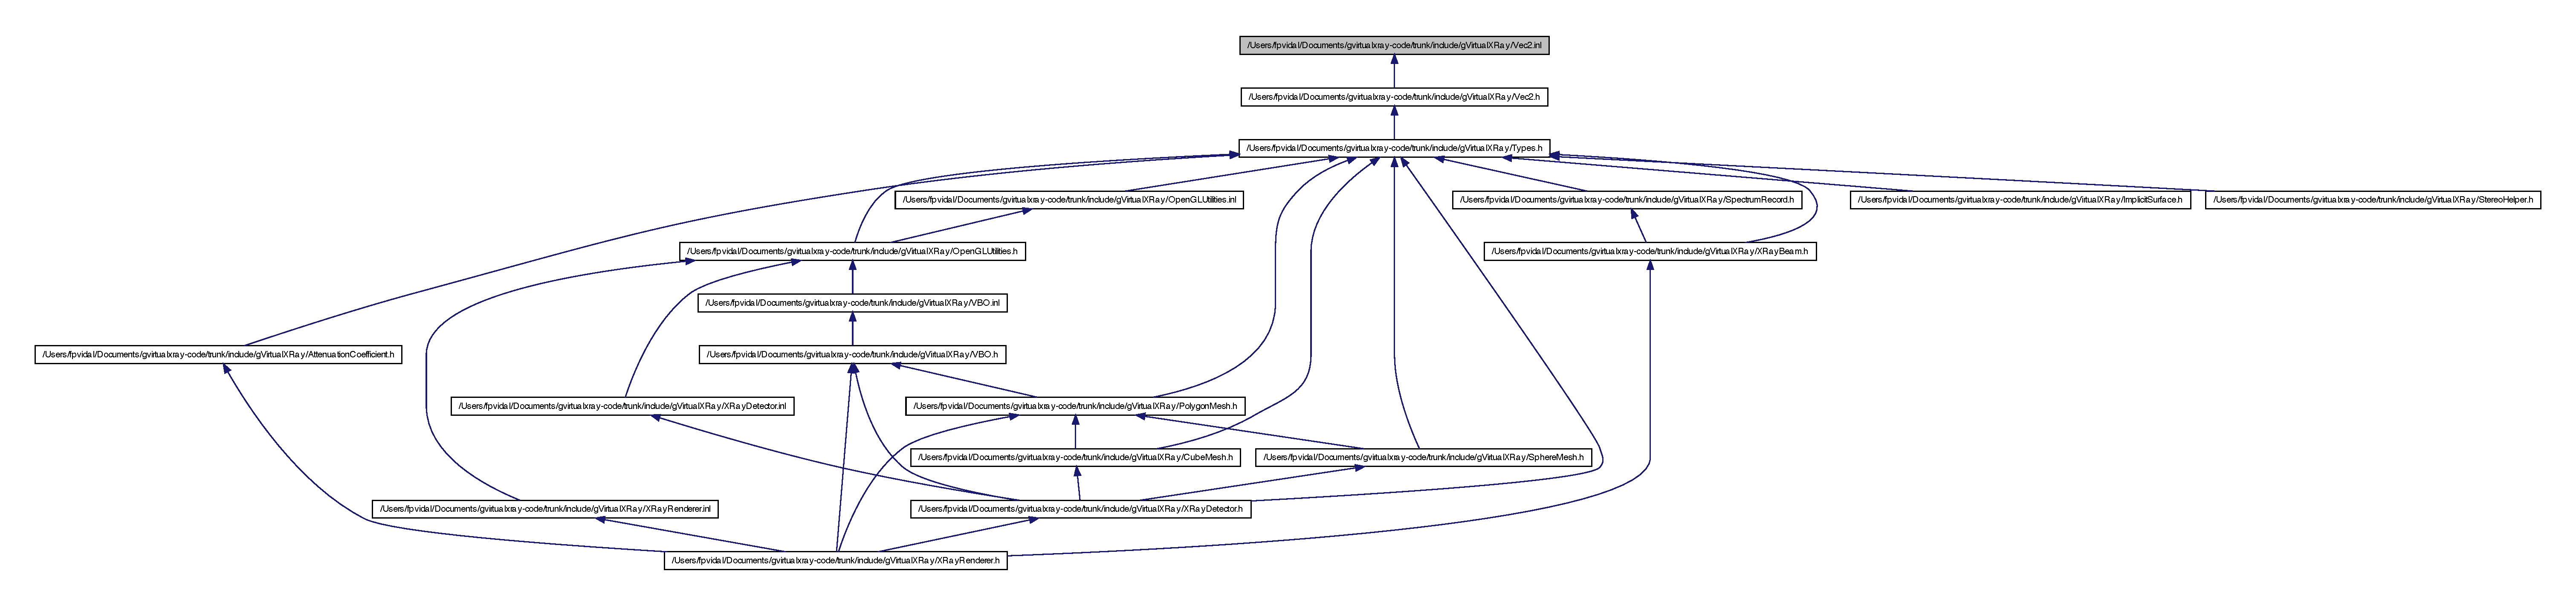
\includegraphics[width=400pt]{_vec2_8inl__dep__incl}
\end{center}
\end{figure}
\subsection*{Namespaces}
\begin{DoxyCompactItemize}
\item 
namespace \hyperlink{namespace_math}{Math}
\end{DoxyCompactItemize}
\subsection*{Functions}
\begin{DoxyCompactItemize}
\item 
{\footnotesize template$<$typename T $>$ }\\std::ostream \& \hyperlink{namespace_math_ae50cf02c21b5ac0d5823b4c241a78e4a}{Math::operator$<$$<$} (std::ostream \&anOutputStream, const Vec2$<$ T $>$ \&aVector)
\end{DoxyCompactItemize}


\subsection{Detailed Description}
Template class to handle 2D vectors. \begin{DoxyVersion}{Version}
1.0
\end{DoxyVersion}
\begin{DoxyDate}{Date}
11/11/2013
\end{DoxyDate}
\begin{DoxyAuthor}{Author}
Dr Franck P. Vidal
\end{DoxyAuthor}
\hypertarget{_x_ray_renderer_8inl_License}{}\subsection{License}\label{_x_ray_renderer_8inl_License}
BSD 3-\/Clause License.

For details on use and redistribution please refer to \href{http://opensource.org/licenses/BSD-3-Clause}{\tt http://opensource.org/licenses/BSD-\/3-\/Clause}\hypertarget{_x_ray_renderer_8inl_Copyright}{}\subsection{Copyright}\label{_x_ray_renderer_8inl_Copyright}
(c) by Dr Franck P. Vidal (\href{mailto:franck.p.vidal@fpvidal.net}{\tt franck.p.vidal@fpvidal.net}), \href{http://www.fpvidal.net/,}{\tt http://www.fpvidal.net/,} Dec 2013, 2013, version 1.0, BSD 3-\/Clause License 

Definition in file \hyperlink{_vec2_8inl_source}{Vec2.inl}.


\hypertarget{_vec3_8h}{
\section{/Users/fpvidal/Documents/gvirtualxray-\/code/trunk/include/gVirtualXRay/Vec3.h File Reference}
\label{_vec3_8h}\index{/Users/fpvidal/Documents/gvirtualxray-\/code/trunk/include/gVirtualXRay/Vec3.h@{/Users/fpvidal/Documents/gvirtualxray-\/code/trunk/include/gVirtualXRay/Vec3.h}}
}


Template class to handle 3D vectors.  


{\ttfamily \#include $<$iostream$>$}\par
{\ttfamily \#include \char`\"{}Vec3.inl\char`\"{}}\par
Include dependency graph for Vec3.h:\nopagebreak
\begin{figure}[H]
\begin{center}
\leavevmode
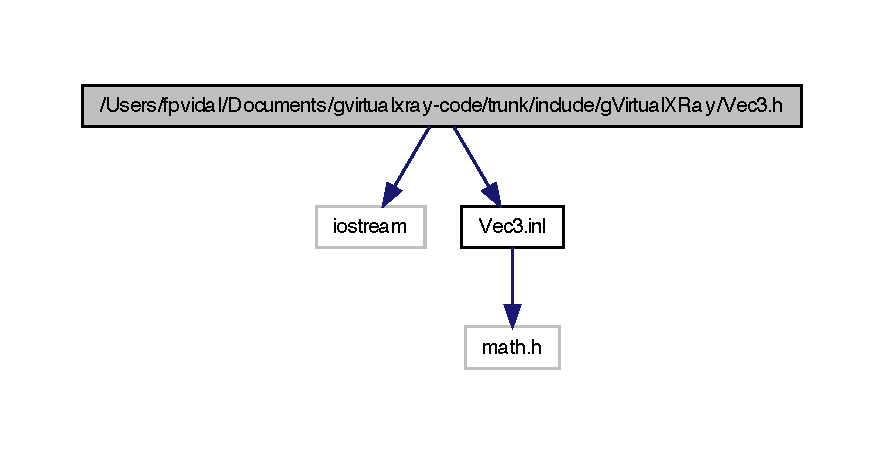
\includegraphics[width=400pt]{_vec3_8h__incl}
\end{center}
\end{figure}
This graph shows which files directly or indirectly include this file:
\nopagebreak
\begin{figure}[H]
\begin{center}
\leavevmode
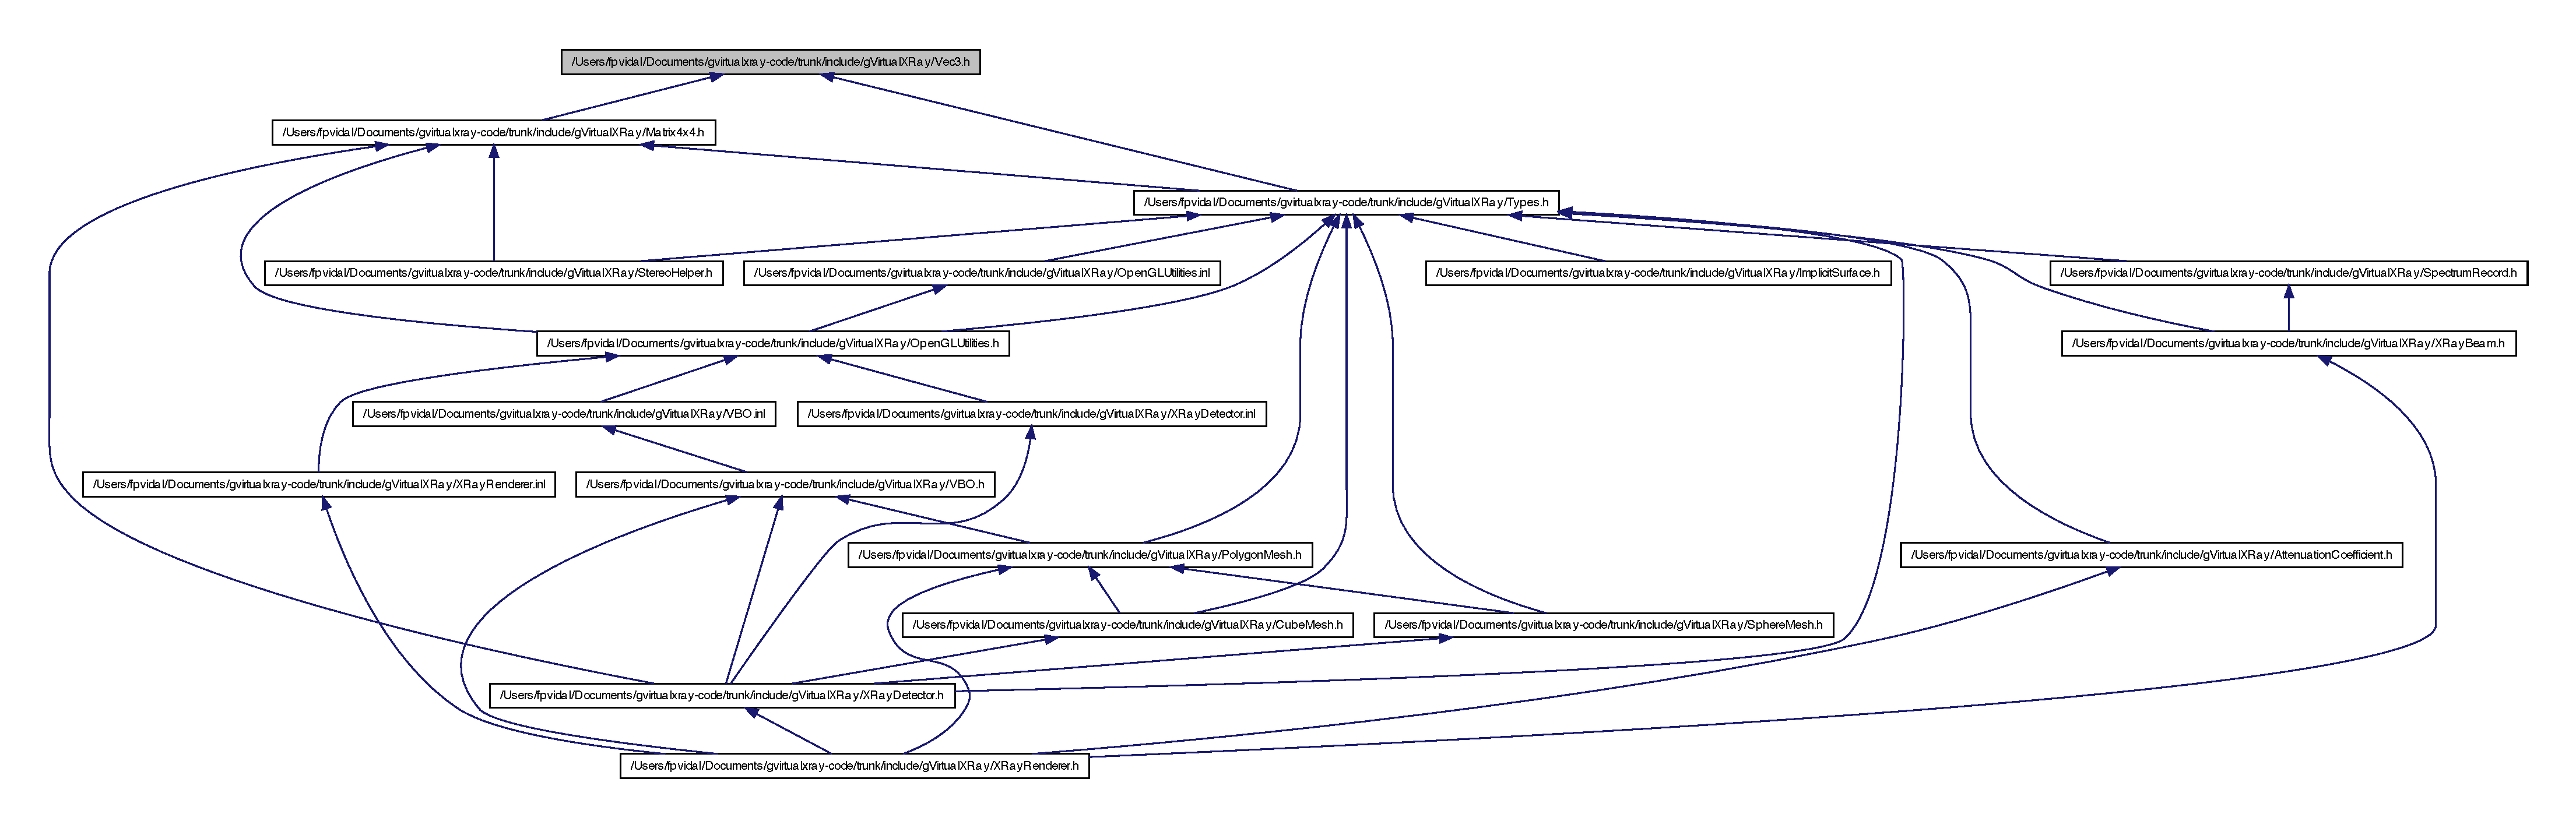
\includegraphics[width=400pt]{_vec3_8h__dep__incl}
\end{center}
\end{figure}
\subsection*{Classes}
\begin{DoxyCompactItemize}
\item 
class \hyperlink{class_math_1_1_vec3}{Math::Vec3$<$ T $>$}
\begin{DoxyCompactList}\small\item\em \hyperlink{class_math_1_1_vec3}{Vec3} is a template class to handle a 3D vector. \end{DoxyCompactList}\end{DoxyCompactItemize}
\subsection*{Namespaces}
\begin{DoxyCompactItemize}
\item 
namespace \hyperlink{namespace_math}{Math}
\end{DoxyCompactItemize}
\subsection*{Functions}
\begin{DoxyCompactItemize}
\item 
{\footnotesize template$<$typename T $>$ }\\std::ostream \& \hyperlink{namespace_math_acc900aa9a1fb3f647f5376f3ef9fd394}{Math::operator$<$$<$} (std::ostream \&anOutputStream, const Vec3$<$ T $>$ \&aVector)
\item 
{\footnotesize template$<$typename T $>$ }\\Vec3$<$ T $>$ \hyperlink{namespace_math_a70ac0d0292ad4baeaf81e8a0bfe92173}{Math::operator$\ast$} (const double \&aValue, const Vec3$<$ T $>$ \&aVector)
\begin{DoxyCompactList}\small\item\em Operator $\ast$ to multiply each component of the vector by a given value. \end{DoxyCompactList}\end{DoxyCompactItemize}


\subsection{Detailed Description}
Template class to handle 3D vectors. \begin{Desc}
\item[\hyperlink{todo__todo000006}{Todo}]Add an exception in Length(). Add a header for constants, use EPSILON instead of 0.0000001\end{Desc}


\begin{DoxyVersion}{Version}
1.0
\end{DoxyVersion}
\begin{DoxyDate}{Date}
11/11/2013
\end{DoxyDate}
\begin{DoxyAuthor}{Author}
Dr Franck P. Vidal
\end{DoxyAuthor}
\hypertarget{_x_ray_renderer_8inl_License}{}\subsection{License}\label{_x_ray_renderer_8inl_License}
BSD 3-\/Clause License.

For details on use and redistribution please refer to \href{http://opensource.org/licenses/BSD-3-Clause}{\tt http://opensource.org/licenses/BSD-\/3-\/Clause}\hypertarget{_x_ray_renderer_8inl_Copyright}{}\subsection{Copyright}\label{_x_ray_renderer_8inl_Copyright}
(c) by Dr Franck P. Vidal (\href{mailto:franck.p.vidal@fpvidal.net}{\tt franck.p.vidal@fpvidal.net}), \href{http://www.fpvidal.net/,}{\tt http://www.fpvidal.net/,} Dec 2013, 2013, version 1.0, BSD 3-\/Clause License 

Definition in file \hyperlink{_vec3_8h_source}{Vec3.h}.


\hypertarget{_vec3_8inl}{
\section{/Users/fpvidal/Documents/gvirtualxray-\/code/trunk/include/gVirtualXRay/Vec3.inl File Reference}
\label{_vec3_8inl}\index{/Users/fpvidal/Documents/gvirtualxray-\/code/trunk/include/gVirtualXRay/Vec3.inl@{/Users/fpvidal/Documents/gvirtualxray-\/code/trunk/include/gVirtualXRay/Vec3.inl}}
}


Template class to handle 3D vectors.  


{\ttfamily \#include $<$math.h$>$}\par
Include dependency graph for Vec3.inl:\nopagebreak
\begin{figure}[H]
\begin{center}
\leavevmode
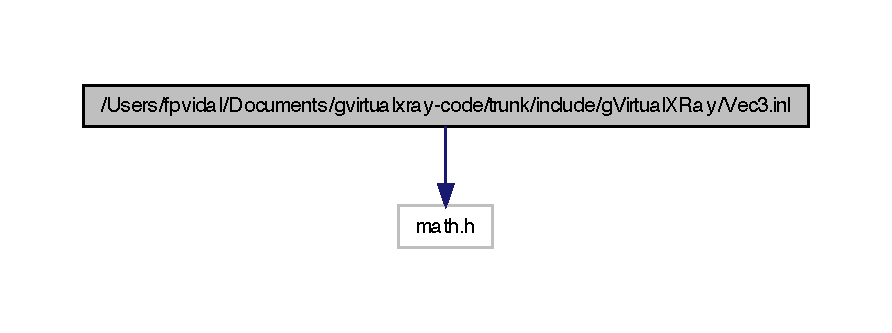
\includegraphics[width=400pt]{_vec3_8inl__incl}
\end{center}
\end{figure}
This graph shows which files directly or indirectly include this file:
\nopagebreak
\begin{figure}[H]
\begin{center}
\leavevmode
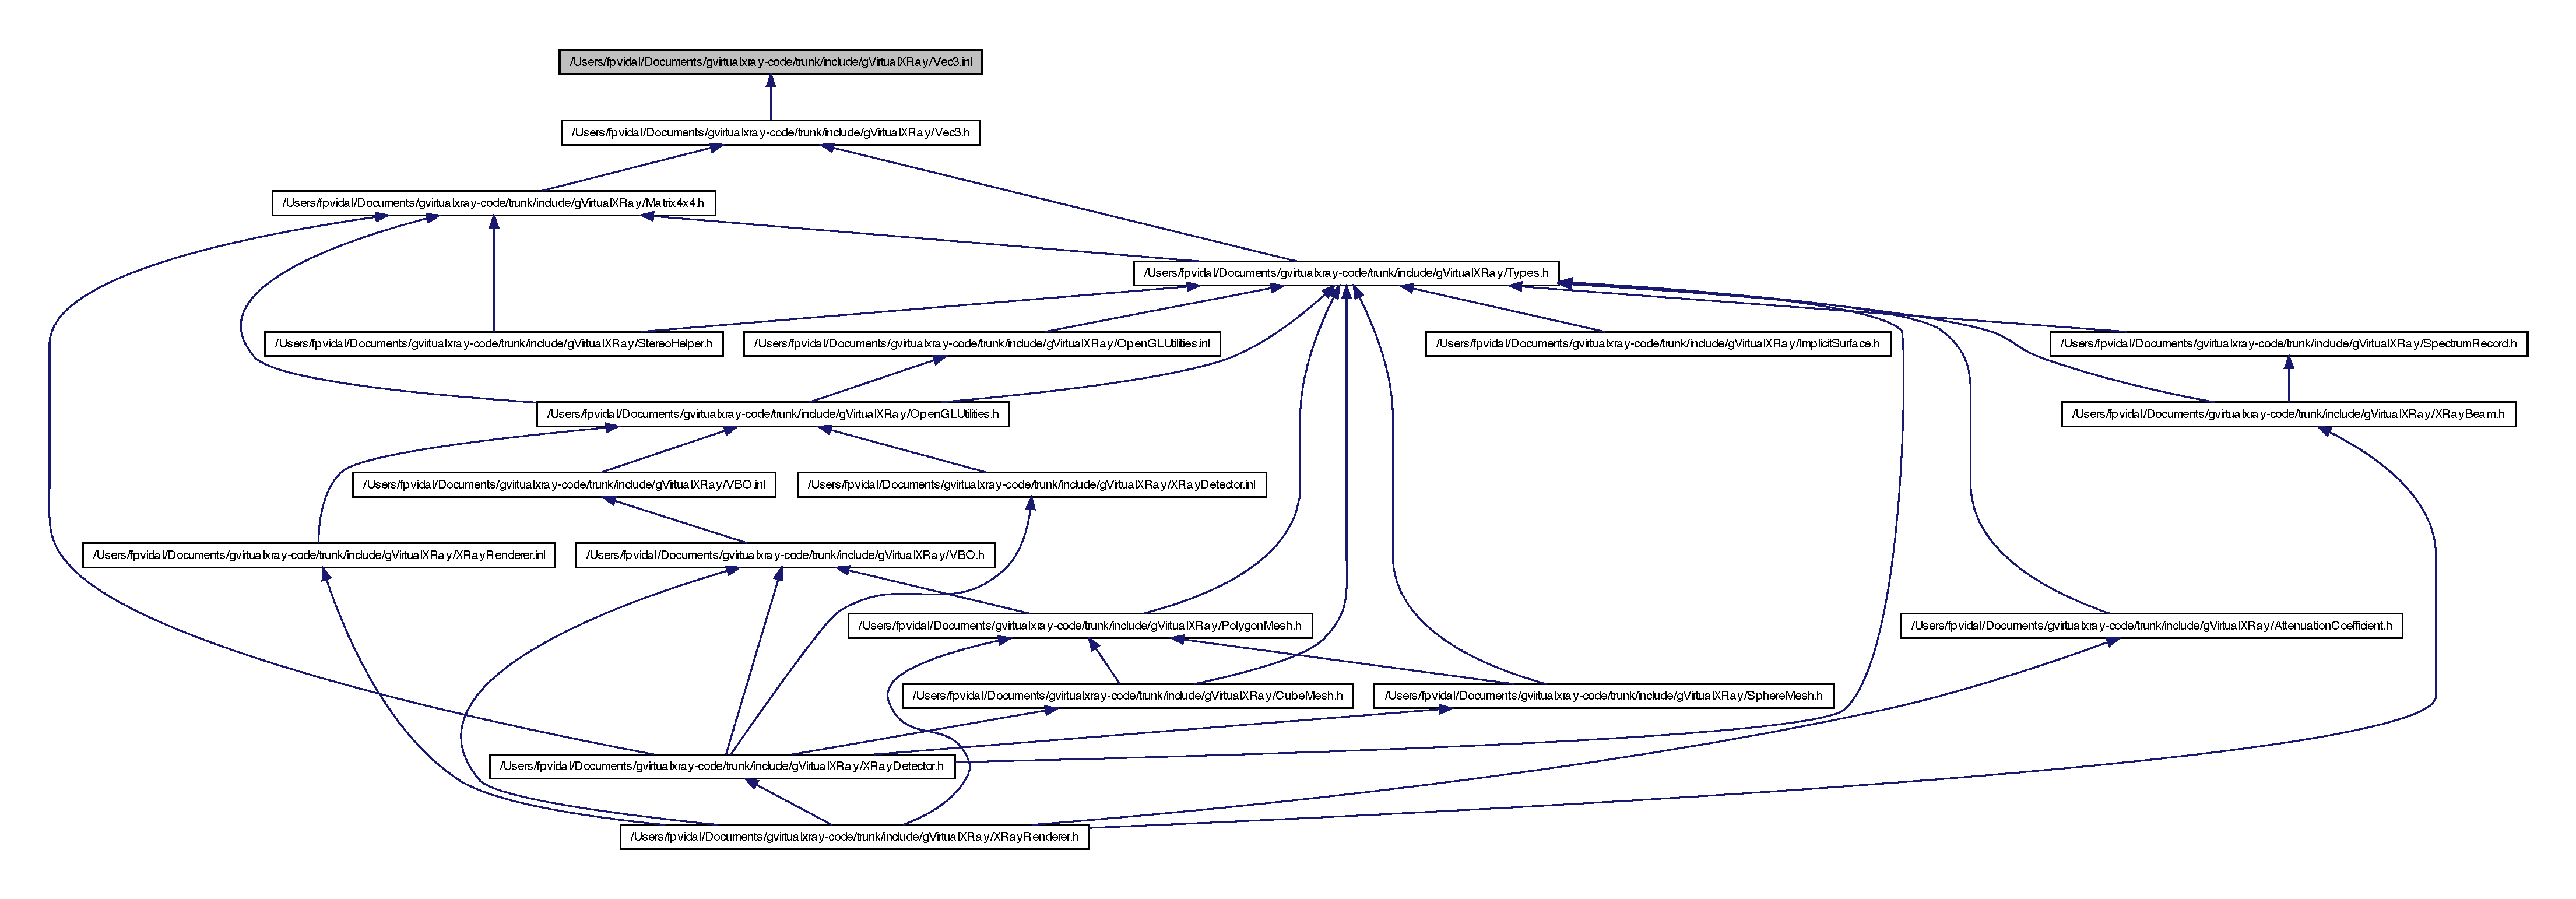
\includegraphics[width=400pt]{_vec3_8inl__dep__incl}
\end{center}
\end{figure}
\subsection*{Namespaces}
\begin{DoxyCompactItemize}
\item 
namespace \hyperlink{namespace_math}{Math}
\end{DoxyCompactItemize}
\subsection*{Functions}
\begin{DoxyCompactItemize}
\item 
{\footnotesize template$<$typename T $>$ }\\Vec3$<$ T $>$ \hyperlink{namespace_math_a70ac0d0292ad4baeaf81e8a0bfe92173}{Math::operator$\ast$} (const double \&aValue, const Vec3$<$ T $>$ \&aVector)
\begin{DoxyCompactList}\small\item\em Operator $\ast$ to multiply each component of the vector by a given value. \end{DoxyCompactList}\item 
{\footnotesize template$<$typename T $>$ }\\std::ostream \& \hyperlink{namespace_math_acc900aa9a1fb3f647f5376f3ef9fd394}{Math::operator$<$$<$} (std::ostream \&anOutputStream, const Vec3$<$ T $>$ \&aVector)
\end{DoxyCompactItemize}


\subsection{Detailed Description}
Template class to handle 3D vectors. \begin{DoxyVersion}{Version}
1.0
\end{DoxyVersion}
\begin{DoxyDate}{Date}
11/11/2013
\end{DoxyDate}
\begin{DoxyAuthor}{Author}
Dr Franck P. Vidal
\end{DoxyAuthor}
\hypertarget{_x_ray_renderer_8inl_License}{}\subsection{License}\label{_x_ray_renderer_8inl_License}
BSD 3-\/Clause License.

For details on use and redistribution please refer to \href{http://opensource.org/licenses/BSD-3-Clause}{\tt http://opensource.org/licenses/BSD-\/3-\/Clause}\hypertarget{_x_ray_renderer_8inl_Copyright}{}\subsection{Copyright}\label{_x_ray_renderer_8inl_Copyright}
(c) by Dr Franck P. Vidal (\href{mailto:franck.p.vidal@fpvidal.net}{\tt franck.p.vidal@fpvidal.net}), \href{http://www.fpvidal.net/,}{\tt http://www.fpvidal.net/,} Dec 2013, 2013, version 1.0, BSD 3-\/Clause License 

Definition in file \hyperlink{_vec3_8inl_source}{Vec3.inl}.


\hypertarget{_x_ray_beam_8h}{
\section{/Users/fpvidal/Documents/gvirtualxray-\/code/trunk/include/gVirtualXRay/XRayBeam.h File Reference}
\label{_x_ray_beam_8h}\index{/Users/fpvidal/Documents/gvirtualxray-\/code/trunk/include/gVirtualXRay/XRayBeam.h@{/Users/fpvidal/Documents/gvirtualxray-\/code/trunk/include/gVirtualXRay/XRayBeam.h}}
}


Class to manage X-\/Ray beams. The beam spectrum is discretised into energy channels.  


{\ttfamily \#include $<$vector$>$}\par
{\ttfamily \#include $<$iostream$>$}\par
{\ttfamily \#include \char`\"{}gVirtualXRay/Types.h\char`\"{}}\par
{\ttfamily \#include \char`\"{}gVirtualXRay/SpectrumRecord.h\char`\"{}}\par
{\ttfamily \#include \char`\"{}XRayBeam.inl\char`\"{}}\par
Include dependency graph for XRayBeam.h:\nopagebreak
\begin{figure}[H]
\begin{center}
\leavevmode
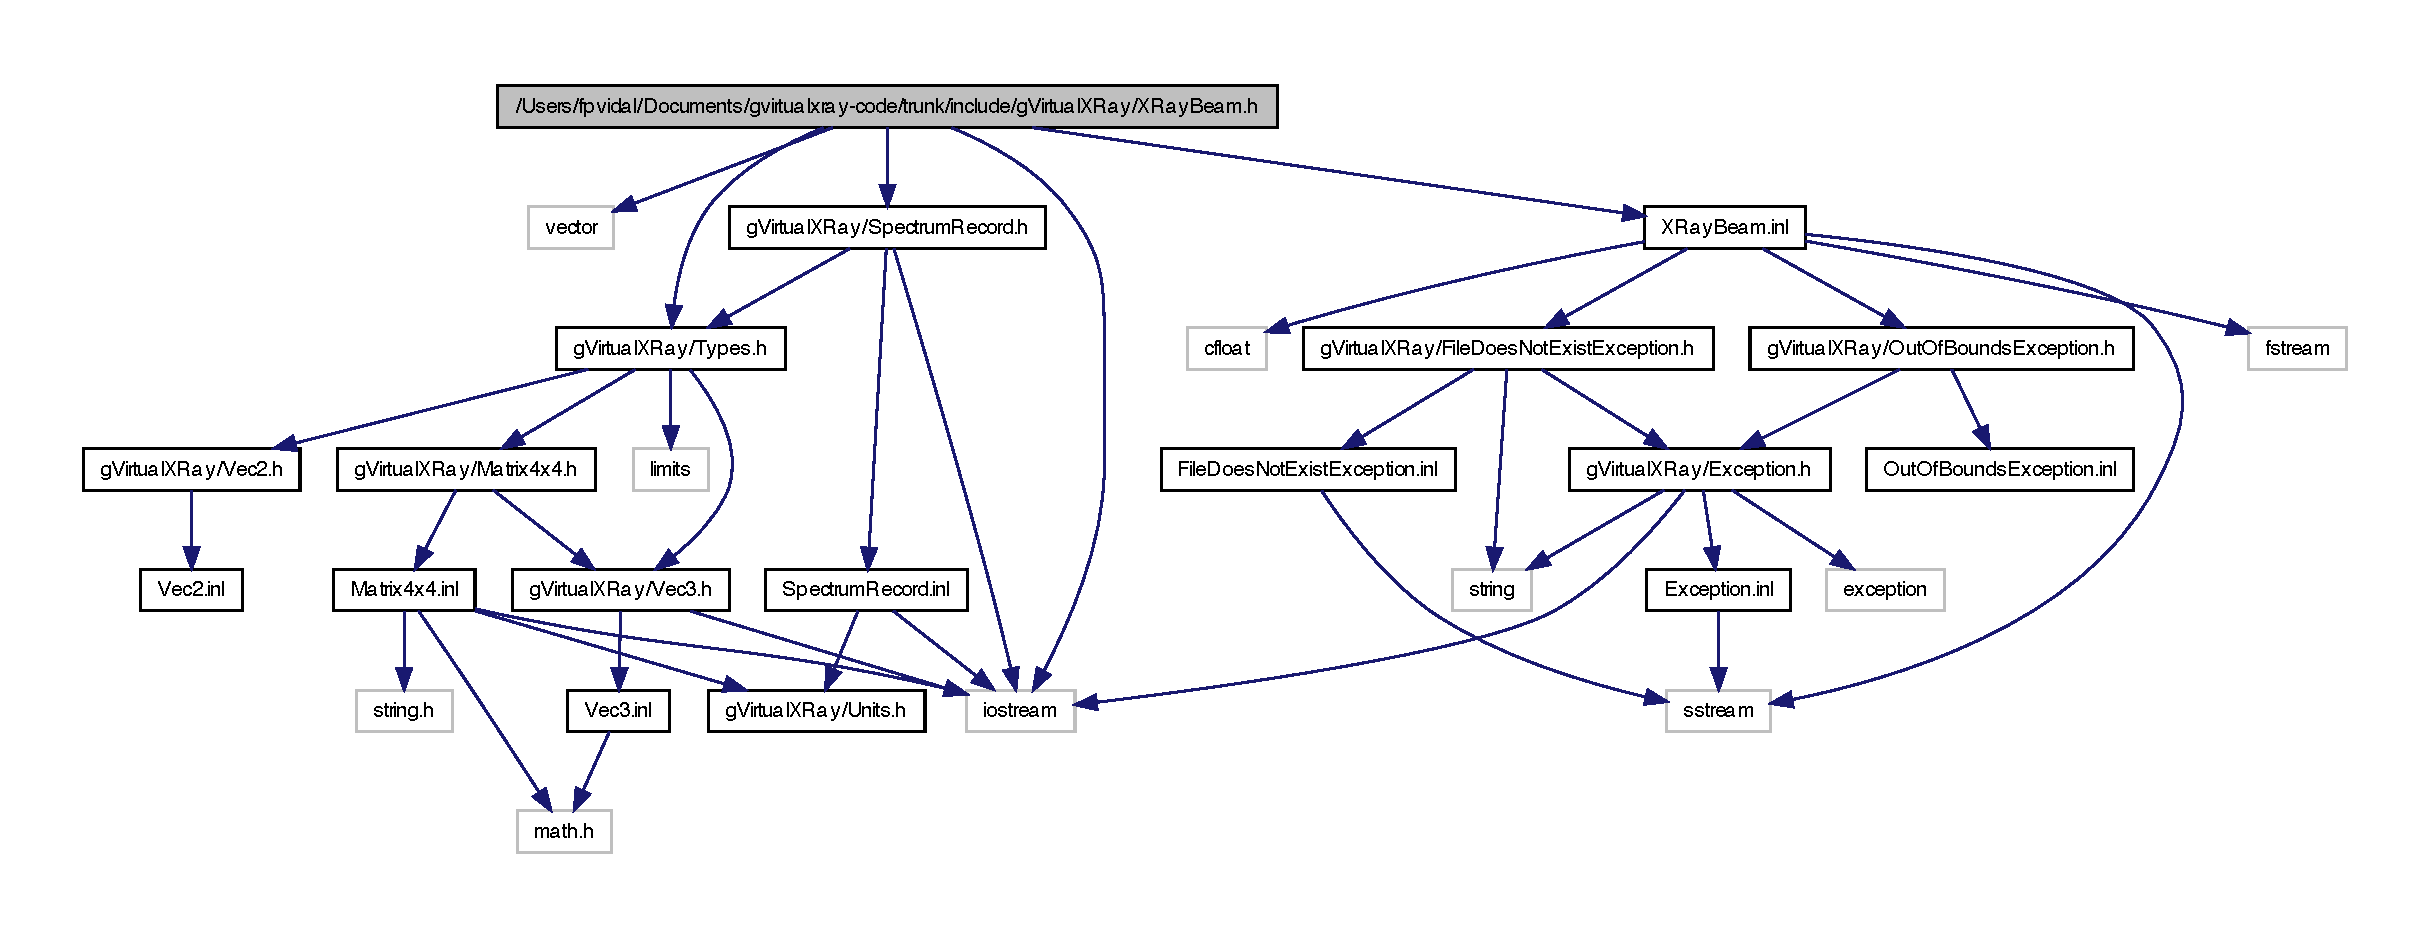
\includegraphics[width=400pt]{_x_ray_beam_8h__incl}
\end{center}
\end{figure}
This graph shows which files directly or indirectly include this file:\nopagebreak
\begin{figure}[H]
\begin{center}
\leavevmode
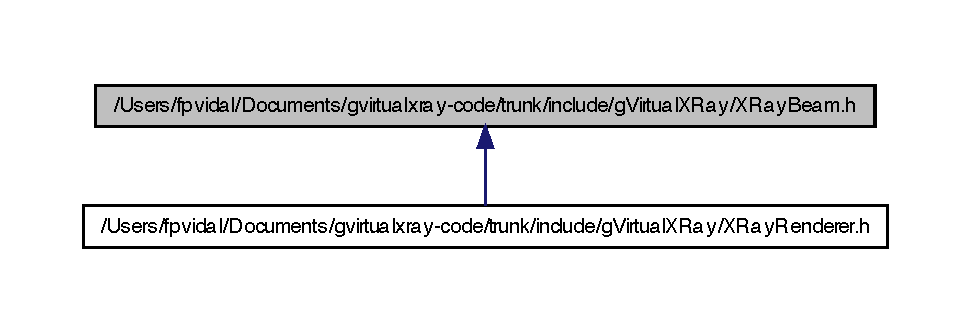
\includegraphics[width=400pt]{_x_ray_beam_8h__dep__incl}
\end{center}
\end{figure}
\subsection*{Classes}
\begin{DoxyCompactItemize}
\item 
class \hyperlink{classg_virtual_x_ray_1_1_x_ray_beam}{gVirtualXRay::XRayBeam}
\begin{DoxyCompactList}\small\item\em \hyperlink{classg_virtual_x_ray_1_1_x_ray_beam}{XRayBeam} is a class to handle the X-\/Ray beam. The beam spectrum is discretised into energy channels. \end{DoxyCompactList}\end{DoxyCompactItemize}
\subsection*{Namespaces}
\begin{DoxyCompactItemize}
\item 
namespace \hyperlink{namespaceg_virtual_x_ray}{gVirtualXRay}
\end{DoxyCompactItemize}


\subsection{Detailed Description}
Class to manage X-\/Ray beams. The beam spectrum is discretised into energy channels. \begin{DoxyVersion}{Version}
1.0
\end{DoxyVersion}
\begin{DoxyDate}{Date}
29/11/2013
\end{DoxyDate}
\begin{DoxyAuthor}{Author}
Dr Franck P. Vidal
\end{DoxyAuthor}
\hypertarget{_x_ray_renderer_8inl_License}{}\subsection{License}\label{_x_ray_renderer_8inl_License}
BSD 3-\/Clause License.

For details on use and redistribution please refer to \href{http://opensource.org/licenses/BSD-3-Clause}{\tt http://opensource.org/licenses/BSD-\/3-\/Clause}\hypertarget{_x_ray_renderer_8inl_Copyright}{}\subsection{Copyright}\label{_x_ray_renderer_8inl_Copyright}
(c) by Dr Franck P. Vidal (\href{mailto:franck.p.vidal@fpvidal.net}{\tt franck.p.vidal@fpvidal.net}), \href{http://www.fpvidal.net/,}{\tt http://www.fpvidal.net/,} Dec 2013, 2013, version 1.0, BSD 3-\/Clause License 

Definition in file \hyperlink{_x_ray_beam_8h_source}{XRayBeam.h}.


\hypertarget{_x_ray_beam_8inl}{
\section{/Users/fpvidal/Documents/gvirtualxray-\/code/trunk/include/gVirtualXRay/XRayBeam.inl File Reference}
\label{_x_ray_beam_8inl}\index{/Users/fpvidal/Documents/gvirtualxray-\/code/trunk/include/gVirtualXRay/XRayBeam.inl@{/Users/fpvidal/Documents/gvirtualxray-\/code/trunk/include/gVirtualXRay/XRayBeam.inl}}
}


Class to manage X-\/Ray beams. The beam spectrum is discretised into energy channels.  


{\ttfamily \#include $<$fstream$>$}\par
{\ttfamily \#include $<$sstream$>$}\par
{\ttfamily \#include $<$cfloat$>$}\par
{\ttfamily \#include \char`\"{}gVirtualXRay/FileDoesNotExistException.h\char`\"{}}\par
{\ttfamily \#include \char`\"{}gVirtualXRay/OutOfBoundsException.h\char`\"{}}\par
Include dependency graph for XRayBeam.inl:\nopagebreak
\begin{figure}[H]
\begin{center}
\leavevmode
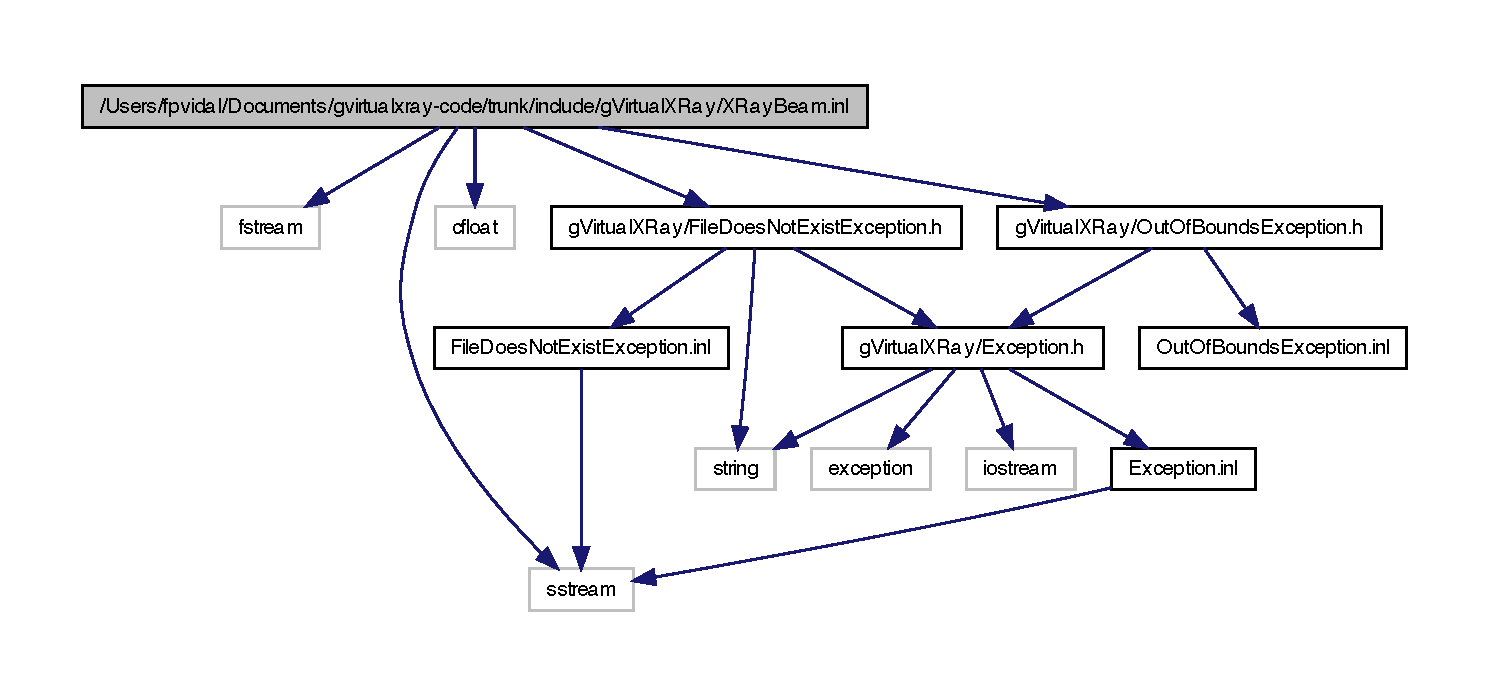
\includegraphics[width=400pt]{_x_ray_beam_8inl__incl}
\end{center}
\end{figure}
This graph shows which files directly or indirectly include this file:\nopagebreak
\begin{figure}[H]
\begin{center}
\leavevmode
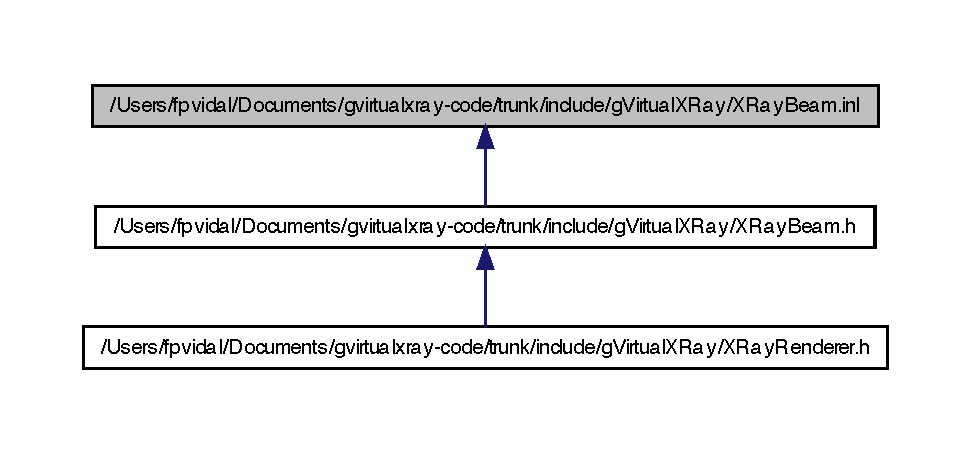
\includegraphics[width=400pt]{_x_ray_beam_8inl__dep__incl}
\end{center}
\end{figure}
\subsection*{Namespaces}
\begin{DoxyCompactItemize}
\item 
namespace \hyperlink{namespaceg_virtual_x_ray}{gVirtualXRay}
\end{DoxyCompactItemize}


\subsection{Detailed Description}
Class to manage X-\/Ray beams. The beam spectrum is discretised into energy channels. \begin{DoxyVersion}{Version}
1.0
\end{DoxyVersion}
\begin{DoxyDate}{Date}
29/11/2013
\end{DoxyDate}
\begin{DoxyAuthor}{Author}
Dr Franck P. Vidal
\end{DoxyAuthor}
\hypertarget{_x_ray_renderer_8inl_License}{}\subsection{License}\label{_x_ray_renderer_8inl_License}
BSD 3-\/Clause License.

For details on use and redistribution please refer to \href{http://opensource.org/licenses/BSD-3-Clause}{\tt http://opensource.org/licenses/BSD-\/3-\/Clause}\hypertarget{_x_ray_renderer_8inl_Copyright}{}\subsection{Copyright}\label{_x_ray_renderer_8inl_Copyright}
(c) by Dr Franck P. Vidal (\href{mailto:franck.p.vidal@fpvidal.net}{\tt franck.p.vidal@fpvidal.net}), \href{http://www.fpvidal.net/,}{\tt http://www.fpvidal.net/,} Dec 2013, 2013, version 1.0, BSD 3-\/Clause License 

Definition in file \hyperlink{_x_ray_beam_8inl_source}{XRayBeam.inl}.


\hypertarget{_x_ray_detector_8h}{
\section{/Users/fpvidal/Documents/gvirtualxray-\/code/trunk/include/gVirtualXRay/XRayDetector.h File Reference}
\label{_x_ray_detector_8h}\index{/Users/fpvidal/Documents/gvirtualxray-\/code/trunk/include/gVirtualXRay/XRayDetector.h@{/Users/fpvidal/Documents/gvirtualxray-\/code/trunk/include/gVirtualXRay/XRayDetector.h}}
}


Class to handle virtual X-\/Ray detectors.  


{\ttfamily \#include \char`\"{}gVirtualXRay/Types.h\char`\"{}}\par
{\ttfamily \#include \char`\"{}gVirtualXRay/Matrix4x4.h\char`\"{}}\par
{\ttfamily \#include \char`\"{}gVirtualXRay/VBO.h\char`\"{}}\par
{\ttfamily \#include \char`\"{}gVirtualXRay/SphereMesh.h\char`\"{}}\par
{\ttfamily \#include \char`\"{}gVirtualXRay/CubeMesh.h\char`\"{}}\par
{\ttfamily \#include \char`\"{}XRayDetector.inl\char`\"{}}\par
Include dependency graph for XRayDetector.h:
\nopagebreak
\begin{figure}[H]
\begin{center}
\leavevmode
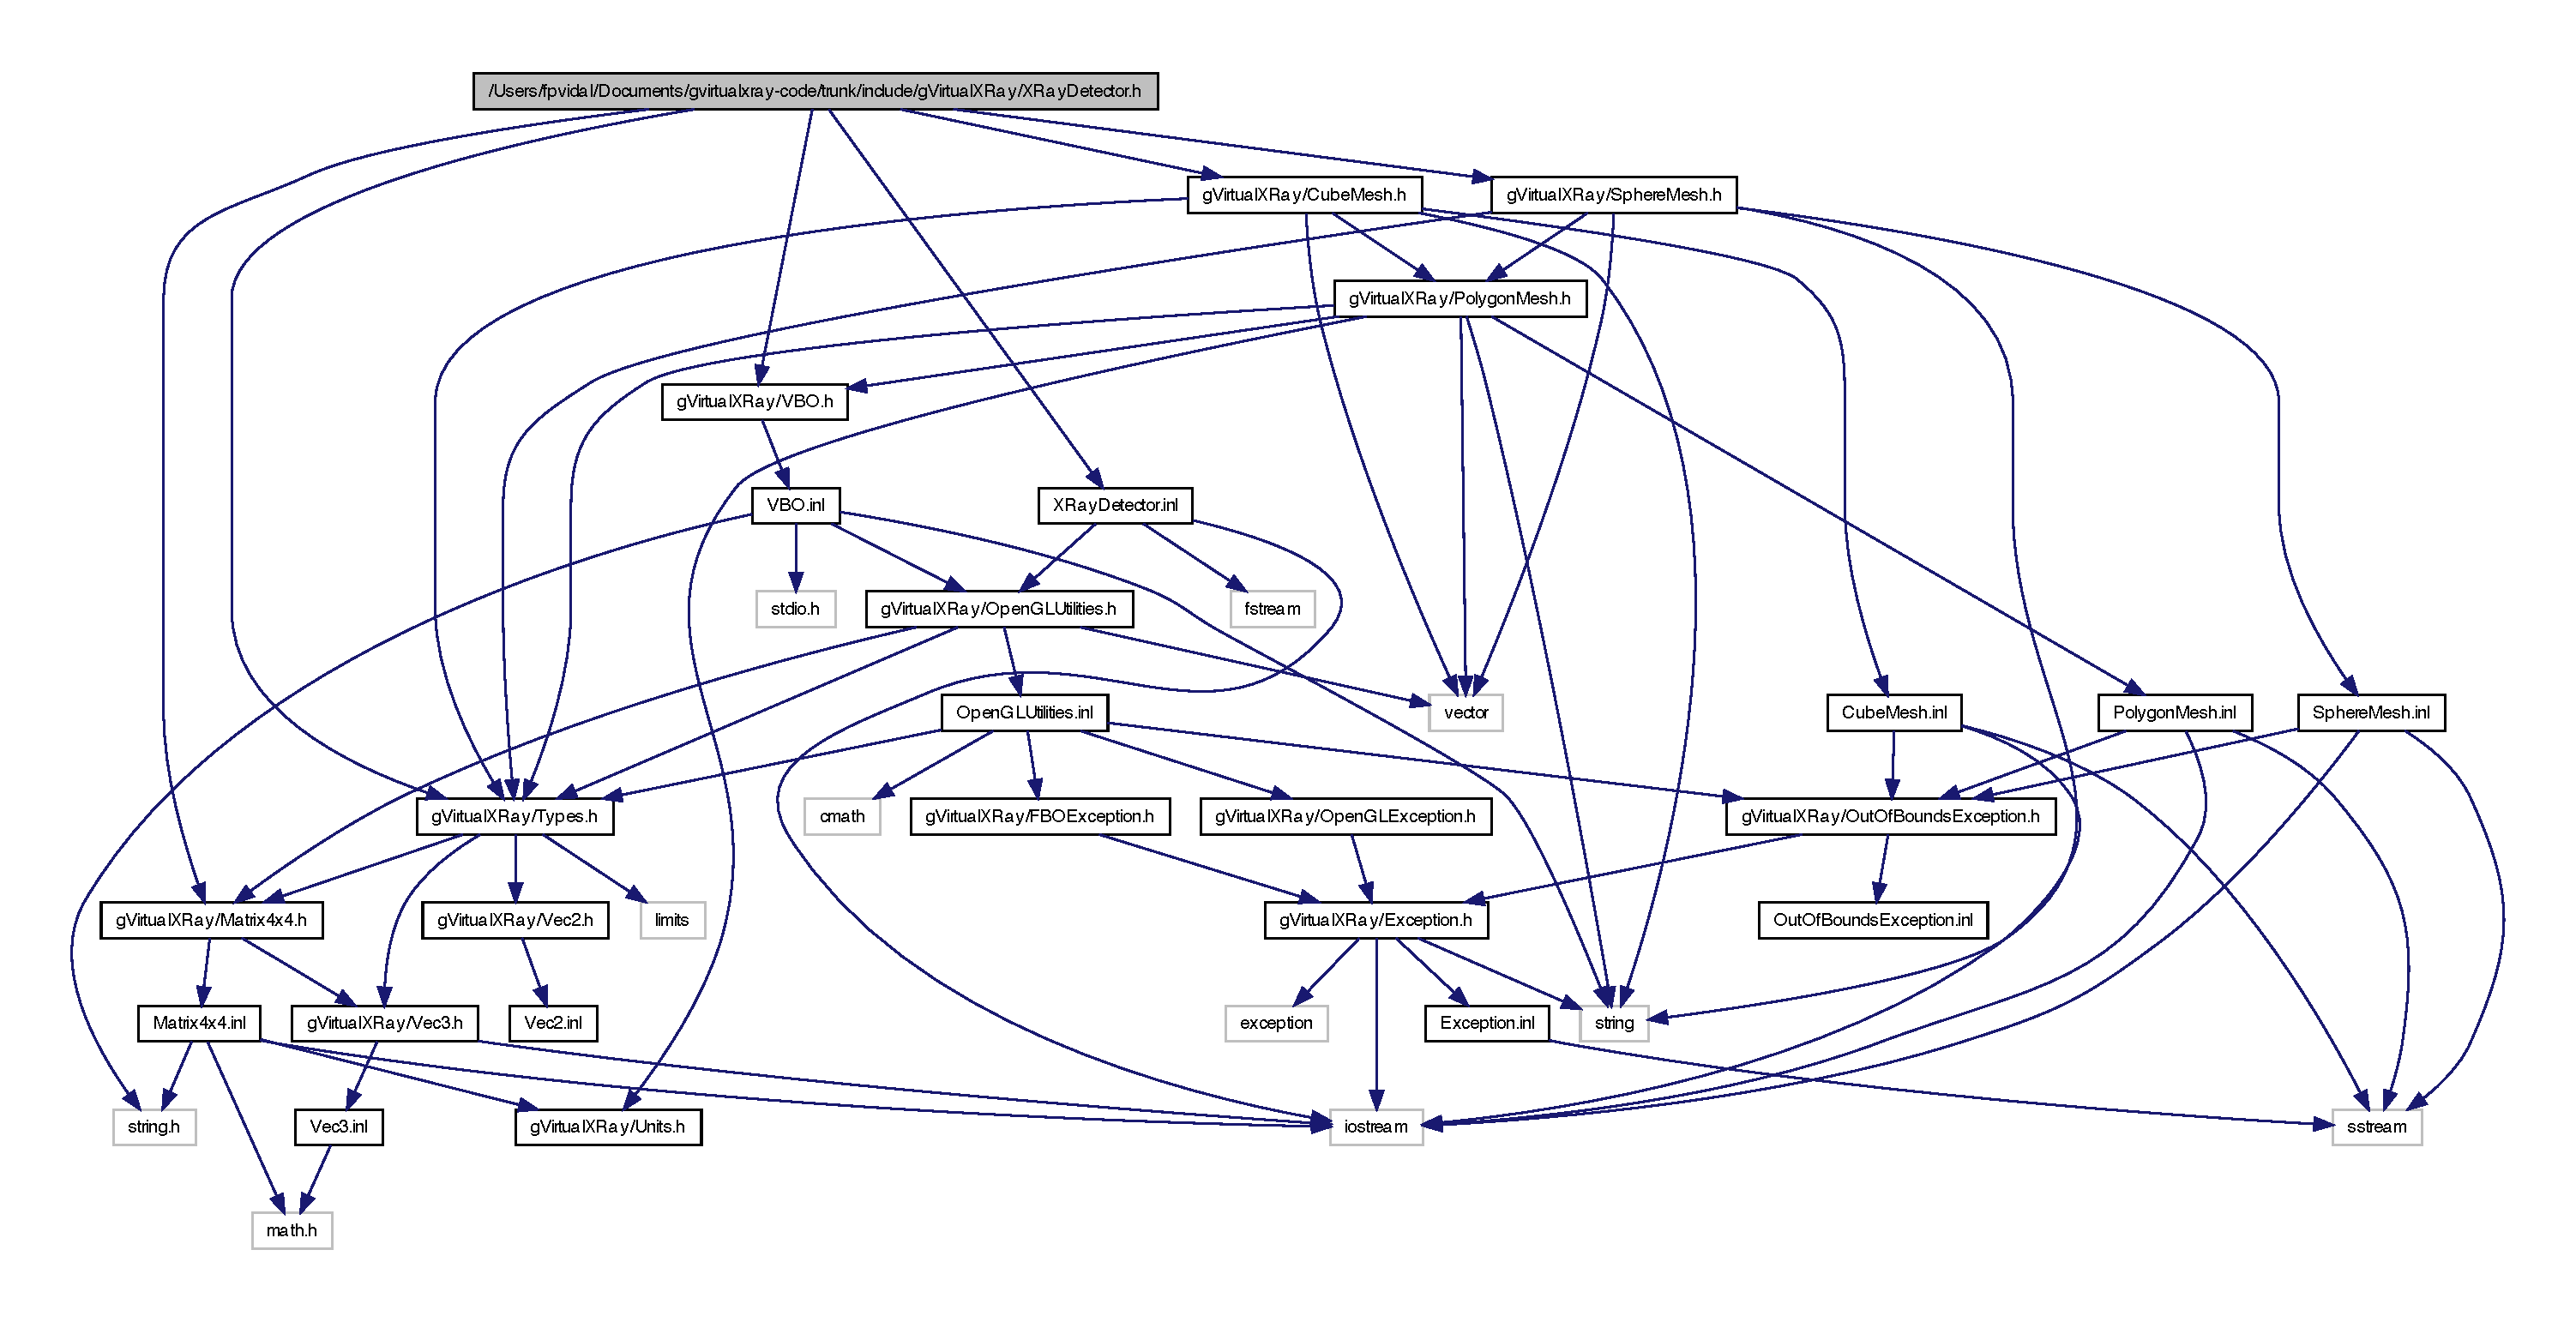
\includegraphics[width=400pt]{_x_ray_detector_8h__incl}
\end{center}
\end{figure}
This graph shows which files directly or indirectly include this file:\nopagebreak
\begin{figure}[H]
\begin{center}
\leavevmode
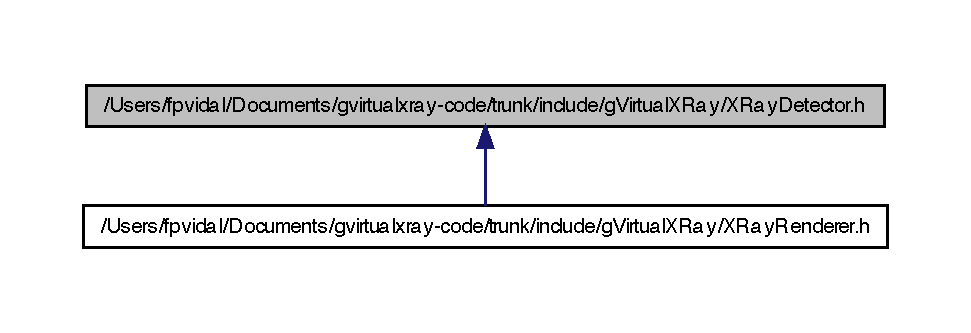
\includegraphics[width=400pt]{_x_ray_detector_8h__dep__incl}
\end{center}
\end{figure}
\subsection*{Classes}
\begin{DoxyCompactItemize}
\item 
class \hyperlink{classg_virtual_x_ray_1_1_x_ray_detector}{gVirtualXRay::XRayDetector}
\begin{DoxyCompactList}\small\item\em \hyperlink{classg_virtual_x_ray_1_1_x_ray_detector}{XRayDetector} is a class to handle a X-\/ray detector. \end{DoxyCompactList}\end{DoxyCompactItemize}
\subsection*{Namespaces}
\begin{DoxyCompactItemize}
\item 
namespace \hyperlink{namespaceg_virtual_x_ray}{gVirtualXRay}
\end{DoxyCompactItemize}


\subsection{Detailed Description}
Class to handle virtual X-\/Ray detectors. \begin{DoxyVersion}{Version}
1.0
\end{DoxyVersion}
\begin{DoxyDate}{Date}
30/11/2013
\end{DoxyDate}
\begin{DoxyAuthor}{Author}
Dr Franck P. Vidal
\end{DoxyAuthor}
\begin{Desc}
\item[\hyperlink{todo__todo000007}{Todo}]Create a class to draw spheres Use this class to display point sources (see line 80 in file \hyperlink{_x_ray_detector_8inl}{XRayDetector.inl})\end{Desc}
\hypertarget{_x_ray_renderer_8inl_License}{}\subsection{License}\label{_x_ray_renderer_8inl_License}
BSD 3-\/Clause License.

For details on use and redistribution please refer to \href{http://opensource.org/licenses/BSD-3-Clause}{\tt http://opensource.org/licenses/BSD-\/3-\/Clause}\hypertarget{_x_ray_renderer_8inl_Copyright}{}\subsection{Copyright}\label{_x_ray_renderer_8inl_Copyright}
(c) by Dr Franck P. Vidal (\href{mailto:franck.p.vidal@fpvidal.net}{\tt franck.p.vidal@fpvidal.net}), \href{http://www.fpvidal.net/,}{\tt http://www.fpvidal.net/,} Dec 2013, 2013, version 1.0, BSD 3-\/Clause License 

Definition in file \hyperlink{_x_ray_detector_8h_source}{XRayDetector.h}.


\hypertarget{_x_ray_detector_8inl}{
\section{/Users/fpvidal/Documents/gvirtualxray-\/code/trunk/include/gVirtualXRay/XRayDetector.inl File Reference}
\label{_x_ray_detector_8inl}\index{/Users/fpvidal/Documents/gvirtualxray-\/code/trunk/include/gVirtualXRay/XRayDetector.inl@{/Users/fpvidal/Documents/gvirtualxray-\/code/trunk/include/gVirtualXRay/XRayDetector.inl}}
}


Class to handle virtual X-\/Ray detectors.  


{\ttfamily \#include $<$fstream$>$}\par
{\ttfamily \#include $<$iostream$>$}\par
{\ttfamily \#include \char`\"{}gVirtualXRay/OpenGLUtilities.h\char`\"{}}\par
Include dependency graph for XRayDetector.inl:\nopagebreak
\begin{figure}[H]
\begin{center}
\leavevmode
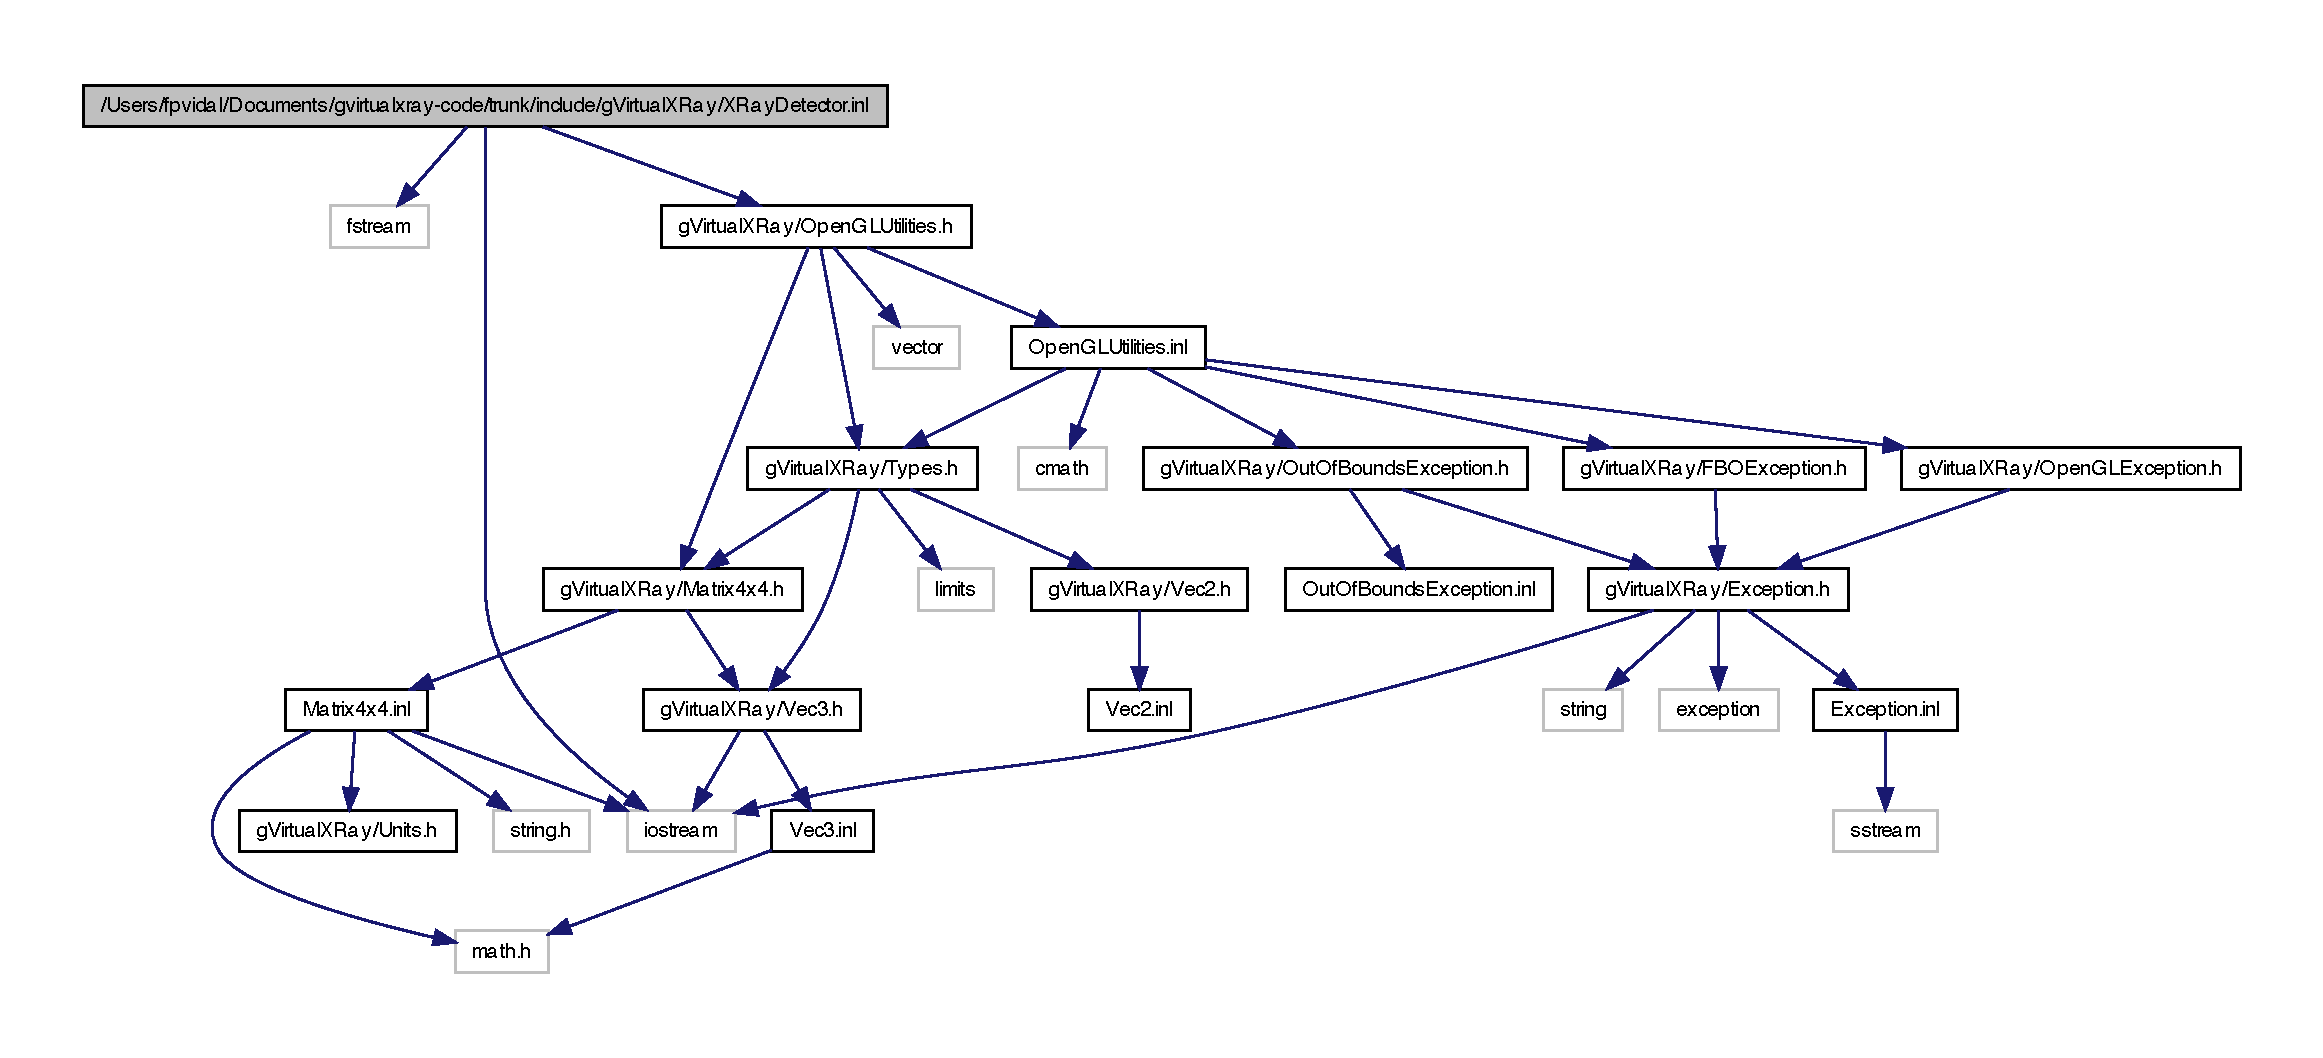
\includegraphics[width=400pt]{_x_ray_detector_8inl__incl}
\end{center}
\end{figure}
This graph shows which files directly or indirectly include this file:\nopagebreak
\begin{figure}[H]
\begin{center}
\leavevmode
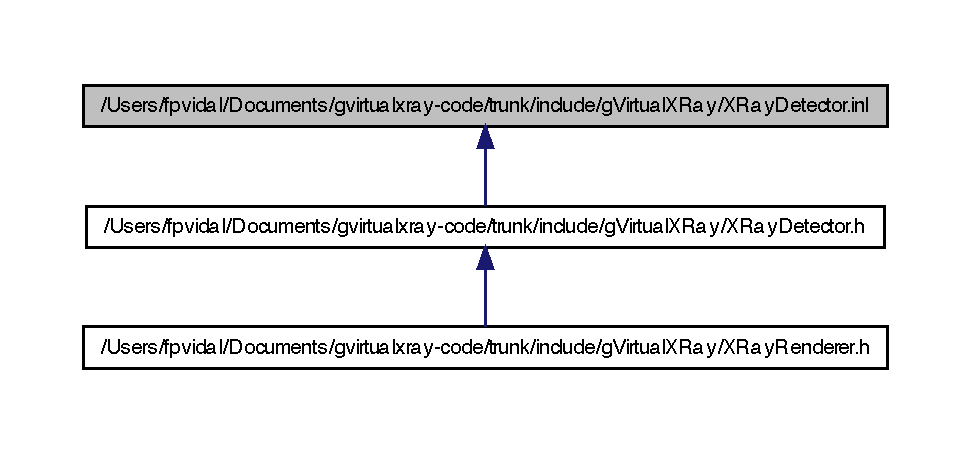
\includegraphics[width=400pt]{_x_ray_detector_8inl__dep__incl}
\end{center}
\end{figure}
\subsection*{Namespaces}
\begin{DoxyCompactItemize}
\item 
namespace \hyperlink{namespaceg_virtual_x_ray}{gVirtualXRay}
\end{DoxyCompactItemize}


\subsection{Detailed Description}
Class to handle virtual X-\/Ray detectors. \begin{DoxyVersion}{Version}
1.0
\end{DoxyVersion}
\begin{DoxyDate}{Date}
30/11/2013
\end{DoxyDate}
\begin{DoxyAuthor}{Author}
Dr Franck P. Vidal
\end{DoxyAuthor}
\hypertarget{_x_ray_renderer_8inl_License}{}\subsection{License}\label{_x_ray_renderer_8inl_License}
BSD 3-\/Clause License.

For details on use and redistribution please refer to \href{http://opensource.org/licenses/BSD-3-Clause}{\tt http://opensource.org/licenses/BSD-\/3-\/Clause}\hypertarget{_x_ray_renderer_8inl_Copyright}{}\subsection{Copyright}\label{_x_ray_renderer_8inl_Copyright}
(c) by Dr Franck P. Vidal (\href{mailto:franck.p.vidal@fpvidal.net}{\tt franck.p.vidal@fpvidal.net}), \href{http://www.fpvidal.net/,}{\tt http://www.fpvidal.net/,} Dec 2013, 2013, version 1.0, BSD 3-\/Clause License 

Definition in file \hyperlink{_x_ray_detector_8inl_source}{XRayDetector.inl}.


\hypertarget{_x_ray_renderer_8h}{
\section{/Users/fpvidal/Documents/gvirtualxray-\/code/trunk/include/gVirtualXRay/XRayRenderer.h File Reference}
\label{_x_ray_renderer_8h}\index{/Users/fpvidal/Documents/gvirtualxray-\/code/trunk/include/gVirtualXRay/XRayRenderer.h@{/Users/fpvidal/Documents/gvirtualxray-\/code/trunk/include/gVirtualXRay/XRayRenderer.h}}
}


Class to compute and renderer X-\/ray images on GPU.  


{\ttfamily \#include $<$vector$>$}\par
{\ttfamily \#include \char`\"{}gVirtualXRay/PolygonMesh.h\char`\"{}}\par
{\ttfamily \#include \char`\"{}gVirtualXRay/XRayDetector.h\char`\"{}}\par
{\ttfamily \#include \char`\"{}gVirtualXRay/XRayBeam.h\char`\"{}}\par
{\ttfamily \#include \char`\"{}gVirtualXRay/Shader.h\char`\"{}}\par
{\ttfamily \#include \char`\"{}gVirtualXRay/AttenuationCoefficient.h\char`\"{}}\par
{\ttfamily \#include \char`\"{}gVirtualXRay/VBO.h\char`\"{}}\par
{\ttfamily \#include \char`\"{}XRayRenderer.inl\char`\"{}}\par
Include dependency graph for XRayRenderer.h:
\nopagebreak
\begin{figure}[H]
\begin{center}
\leavevmode
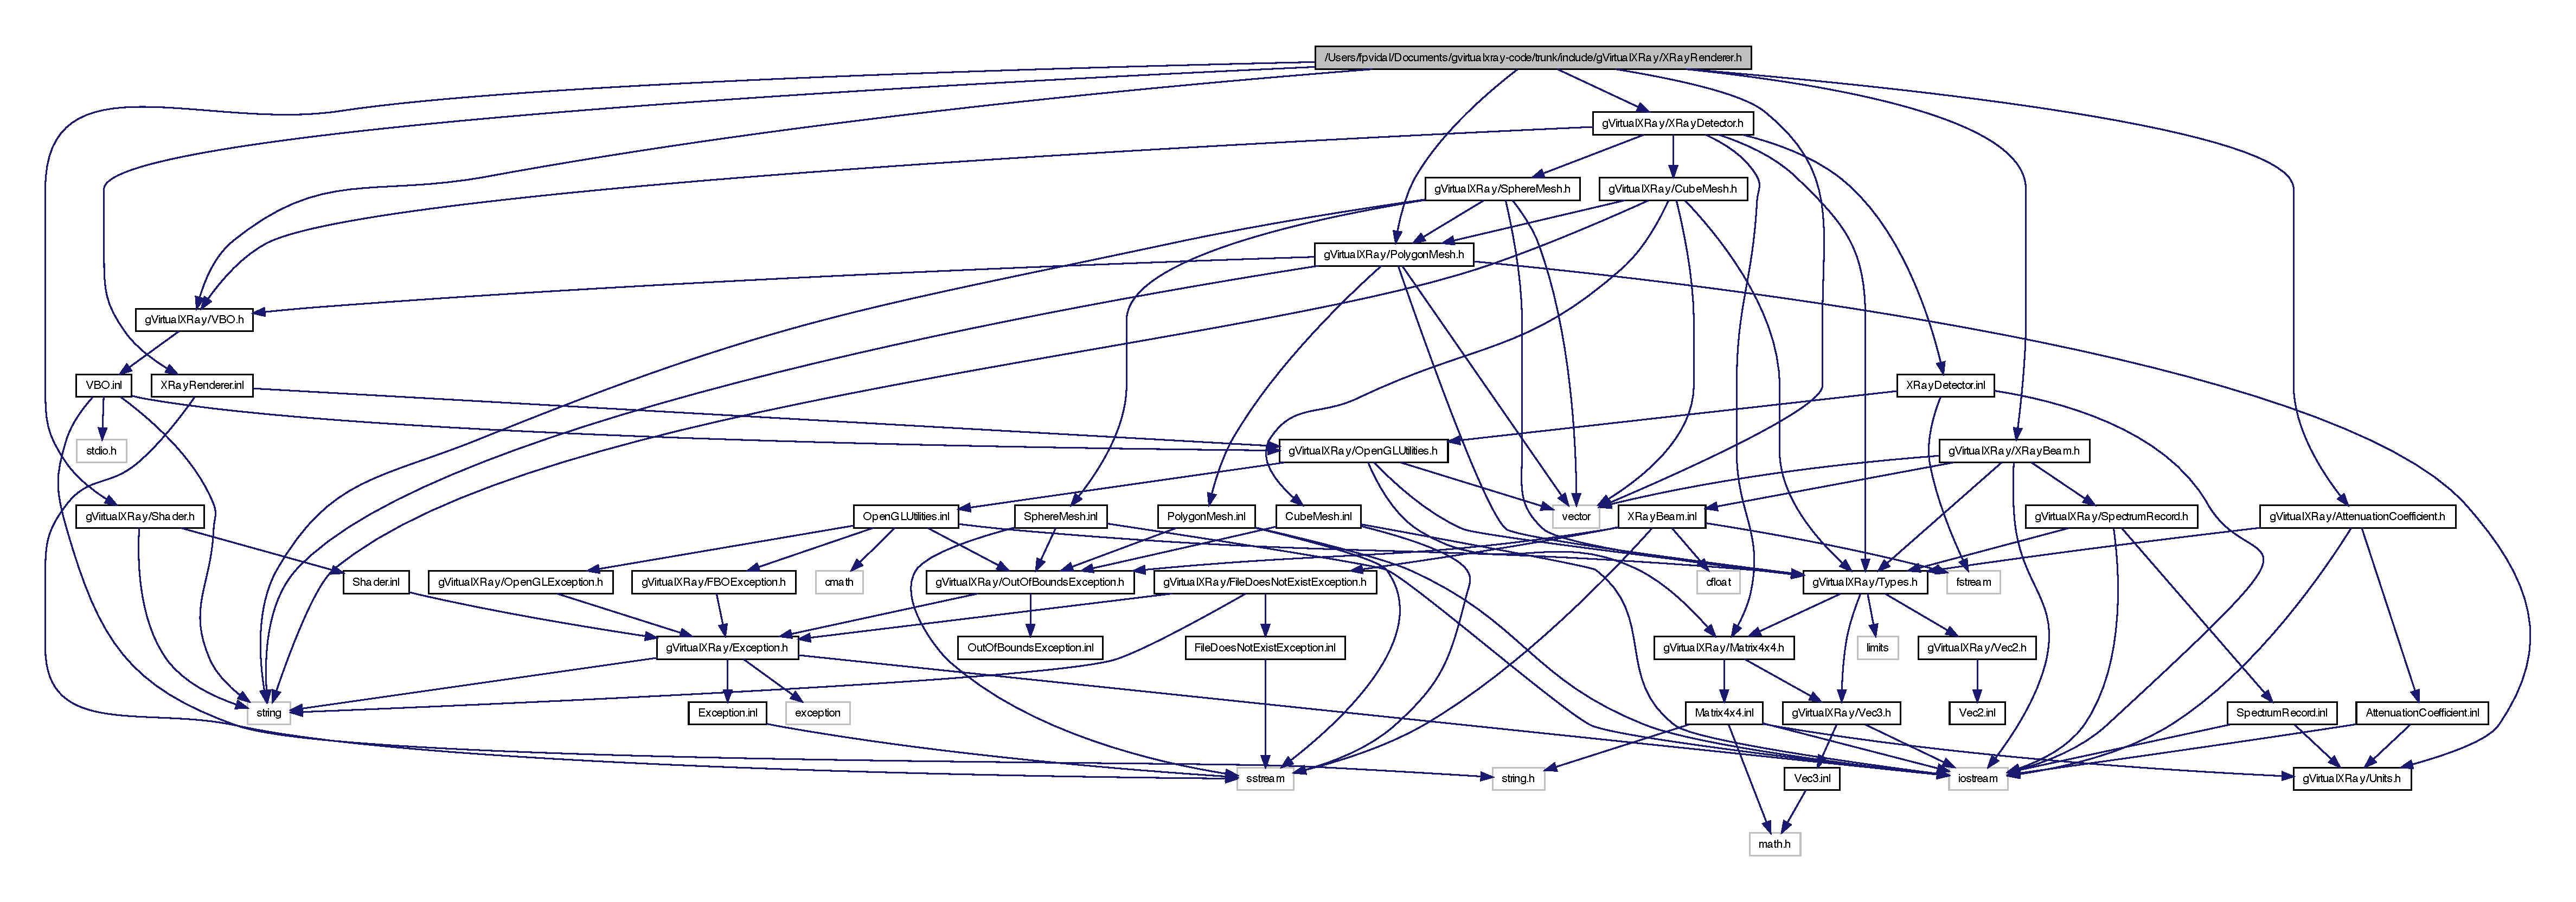
\includegraphics[width=400pt]{_x_ray_renderer_8h__incl}
\end{center}
\end{figure}
\subsection*{Classes}
\begin{DoxyCompactItemize}
\item 
class \hyperlink{classg_virtual_x_ray_1_1_x_ray_renderer}{gVirtualXRay::XRayRenderer}
\begin{DoxyCompactList}\small\item\em \hyperlink{classg_virtual_x_ray_1_1_x_ray_renderer}{XRayRenderer} is a class to compute and renderer X-\/ray images on GPU. \end{DoxyCompactList}\end{DoxyCompactItemize}
\subsection*{Namespaces}
\begin{DoxyCompactItemize}
\item 
namespace \hyperlink{namespaceg_virtual_x_ray}{gVirtualXRay}
\end{DoxyCompactItemize}
\subsection*{Defines}
\begin{DoxyCompactItemize}
\item 
\#define \hyperlink{_x_ray_renderer_8h_a9ae4274c2504cc04ce6825be207e6f1c}{XRAY\_\-DETECTOR\_\-PBO\_\-NUMBER}~2
\begin{DoxyCompactList}\small\item\em The total number of PBOs. \end{DoxyCompactList}\item 
\#define \hyperlink{_x_ray_renderer_8h_a3026db3ec2bc1ff1c683d45b2fb1ccb1}{XRAY\_\-DETECTOR\_\-2D\_\-TEXTURE\_\-NUMBER}~3
\begin{DoxyCompactList}\small\item\em The total number of 2D textures. \end{DoxyCompactList}\item 
\#define \hyperlink{_x_ray_renderer_8h_a78c4f391a360ef8d730500490a2d31c5}{XRAY\_\-DETECTOR\_\-3D\_\-TEXTURE\_\-NUMBER}~1
\begin{DoxyCompactList}\small\item\em The total number of 3D textures. \end{DoxyCompactList}\item 
\#define \hyperlink{_x_ray_renderer_8h_afc8224056b06f62ef628a3ab32ccbe0b}{XRAY\_\-DETECTOR\_\-SHADER\_\-NUMBER}~6
\begin{DoxyCompactList}\small\item\em The total number of program shaders. \end{DoxyCompactList}\end{DoxyCompactItemize}


\subsection{Detailed Description}
Class to compute and renderer X-\/ray images on GPU. \begin{DoxyVersion}{Version}
1.0
\end{DoxyVersion}
\begin{DoxyDate}{Date}
01/12/2013
\end{DoxyDate}
\begin{DoxyAuthor}{Author}
Dr Franck P. Vidal
\end{DoxyAuthor}
\hypertarget{_x_ray_renderer_8inl_License}{}\subsection{License}\label{_x_ray_renderer_8inl_License}
BSD 3-\/Clause License.

For details on use and redistribution please refer to \href{http://opensource.org/licenses/BSD-3-Clause}{\tt http://opensource.org/licenses/BSD-\/3-\/Clause}\hypertarget{_x_ray_renderer_8inl_Copyright}{}\subsection{Copyright}\label{_x_ray_renderer_8inl_Copyright}
(c) by Dr Franck P. Vidal (\href{mailto:franck.p.vidal@fpvidal.net}{\tt franck.p.vidal@fpvidal.net}), \href{http://www.fpvidal.net/,}{\tt http://www.fpvidal.net/,} Dec 2013, 2013, version 1.0, BSD 3-\/Clause License 

Definition in file \hyperlink{_x_ray_renderer_8h_source}{XRayRenderer.h}.



\subsection{Define Documentation}
\hypertarget{_x_ray_renderer_8h_a3026db3ec2bc1ff1c683d45b2fb1ccb1}{
\index{XRayRenderer.h@{XRayRenderer.h}!XRAY\_\-DETECTOR\_\-2D\_\-TEXTURE\_\-NUMBER@{XRAY\_\-DETECTOR\_\-2D\_\-TEXTURE\_\-NUMBER}}
\index{XRAY\_\-DETECTOR\_\-2D\_\-TEXTURE\_\-NUMBER@{XRAY\_\-DETECTOR\_\-2D\_\-TEXTURE\_\-NUMBER}!XRayRenderer.h@{XRayRenderer.h}}
\subsubsection[{XRAY\_\-DETECTOR\_\-2D\_\-TEXTURE\_\-NUMBER}]{\setlength{\rightskip}{0pt plus 5cm}\#define XRAY\_\-DETECTOR\_\-2D\_\-TEXTURE\_\-NUMBER~3}}
\label{_x_ray_renderer_8h_a3026db3ec2bc1ff1c683d45b2fb1ccb1}


The total number of 2D textures. 



Definition at line 72 of file XRayRenderer.h.

\hypertarget{_x_ray_renderer_8h_a78c4f391a360ef8d730500490a2d31c5}{
\index{XRayRenderer.h@{XRayRenderer.h}!XRAY\_\-DETECTOR\_\-3D\_\-TEXTURE\_\-NUMBER@{XRAY\_\-DETECTOR\_\-3D\_\-TEXTURE\_\-NUMBER}}
\index{XRAY\_\-DETECTOR\_\-3D\_\-TEXTURE\_\-NUMBER@{XRAY\_\-DETECTOR\_\-3D\_\-TEXTURE\_\-NUMBER}!XRayRenderer.h@{XRayRenderer.h}}
\subsubsection[{XRAY\_\-DETECTOR\_\-3D\_\-TEXTURE\_\-NUMBER}]{\setlength{\rightskip}{0pt plus 5cm}\#define XRAY\_\-DETECTOR\_\-3D\_\-TEXTURE\_\-NUMBER~1}}
\label{_x_ray_renderer_8h_a78c4f391a360ef8d730500490a2d31c5}


The total number of 3D textures. 



Definition at line 73 of file XRayRenderer.h.

\hypertarget{_x_ray_renderer_8h_a9ae4274c2504cc04ce6825be207e6f1c}{
\index{XRayRenderer.h@{XRayRenderer.h}!XRAY\_\-DETECTOR\_\-PBO\_\-NUMBER@{XRAY\_\-DETECTOR\_\-PBO\_\-NUMBER}}
\index{XRAY\_\-DETECTOR\_\-PBO\_\-NUMBER@{XRAY\_\-DETECTOR\_\-PBO\_\-NUMBER}!XRayRenderer.h@{XRayRenderer.h}}
\subsubsection[{XRAY\_\-DETECTOR\_\-PBO\_\-NUMBER}]{\setlength{\rightskip}{0pt plus 5cm}\#define XRAY\_\-DETECTOR\_\-PBO\_\-NUMBER~2}}
\label{_x_ray_renderer_8h_a9ae4274c2504cc04ce6825be207e6f1c}


The total number of PBOs. 



Definition at line 71 of file XRayRenderer.h.

\hypertarget{_x_ray_renderer_8h_afc8224056b06f62ef628a3ab32ccbe0b}{
\index{XRayRenderer.h@{XRayRenderer.h}!XRAY\_\-DETECTOR\_\-SHADER\_\-NUMBER@{XRAY\_\-DETECTOR\_\-SHADER\_\-NUMBER}}
\index{XRAY\_\-DETECTOR\_\-SHADER\_\-NUMBER@{XRAY\_\-DETECTOR\_\-SHADER\_\-NUMBER}!XRayRenderer.h@{XRayRenderer.h}}
\subsubsection[{XRAY\_\-DETECTOR\_\-SHADER\_\-NUMBER}]{\setlength{\rightskip}{0pt plus 5cm}\#define XRAY\_\-DETECTOR\_\-SHADER\_\-NUMBER~6}}
\label{_x_ray_renderer_8h_afc8224056b06f62ef628a3ab32ccbe0b}


The total number of program shaders. 



Definition at line 74 of file XRayRenderer.h.


\hypertarget{_x_ray_renderer_8inl}{
\section{/Users/fpvidal/Documents/gvirtualxray-\/code/trunk/include/gVirtualXRay/XRayRenderer.inl File Reference}
\label{_x_ray_renderer_8inl}\index{/Users/fpvidal/Documents/gvirtualxray-\/code/trunk/include/gVirtualXRay/XRayRenderer.inl@{/Users/fpvidal/Documents/gvirtualxray-\/code/trunk/include/gVirtualXRay/XRayRenderer.inl}}
}


Class to compute and renderer X-\/ray images on GPU.  


{\ttfamily \#include $<$sstream$>$}\par
{\ttfamily \#include \char`\"{}gVirtualXRay/OpenGLUtilities.h\char`\"{}}\par
Include dependency graph for XRayRenderer.inl:\nopagebreak
\begin{figure}[H]
\begin{center}
\leavevmode
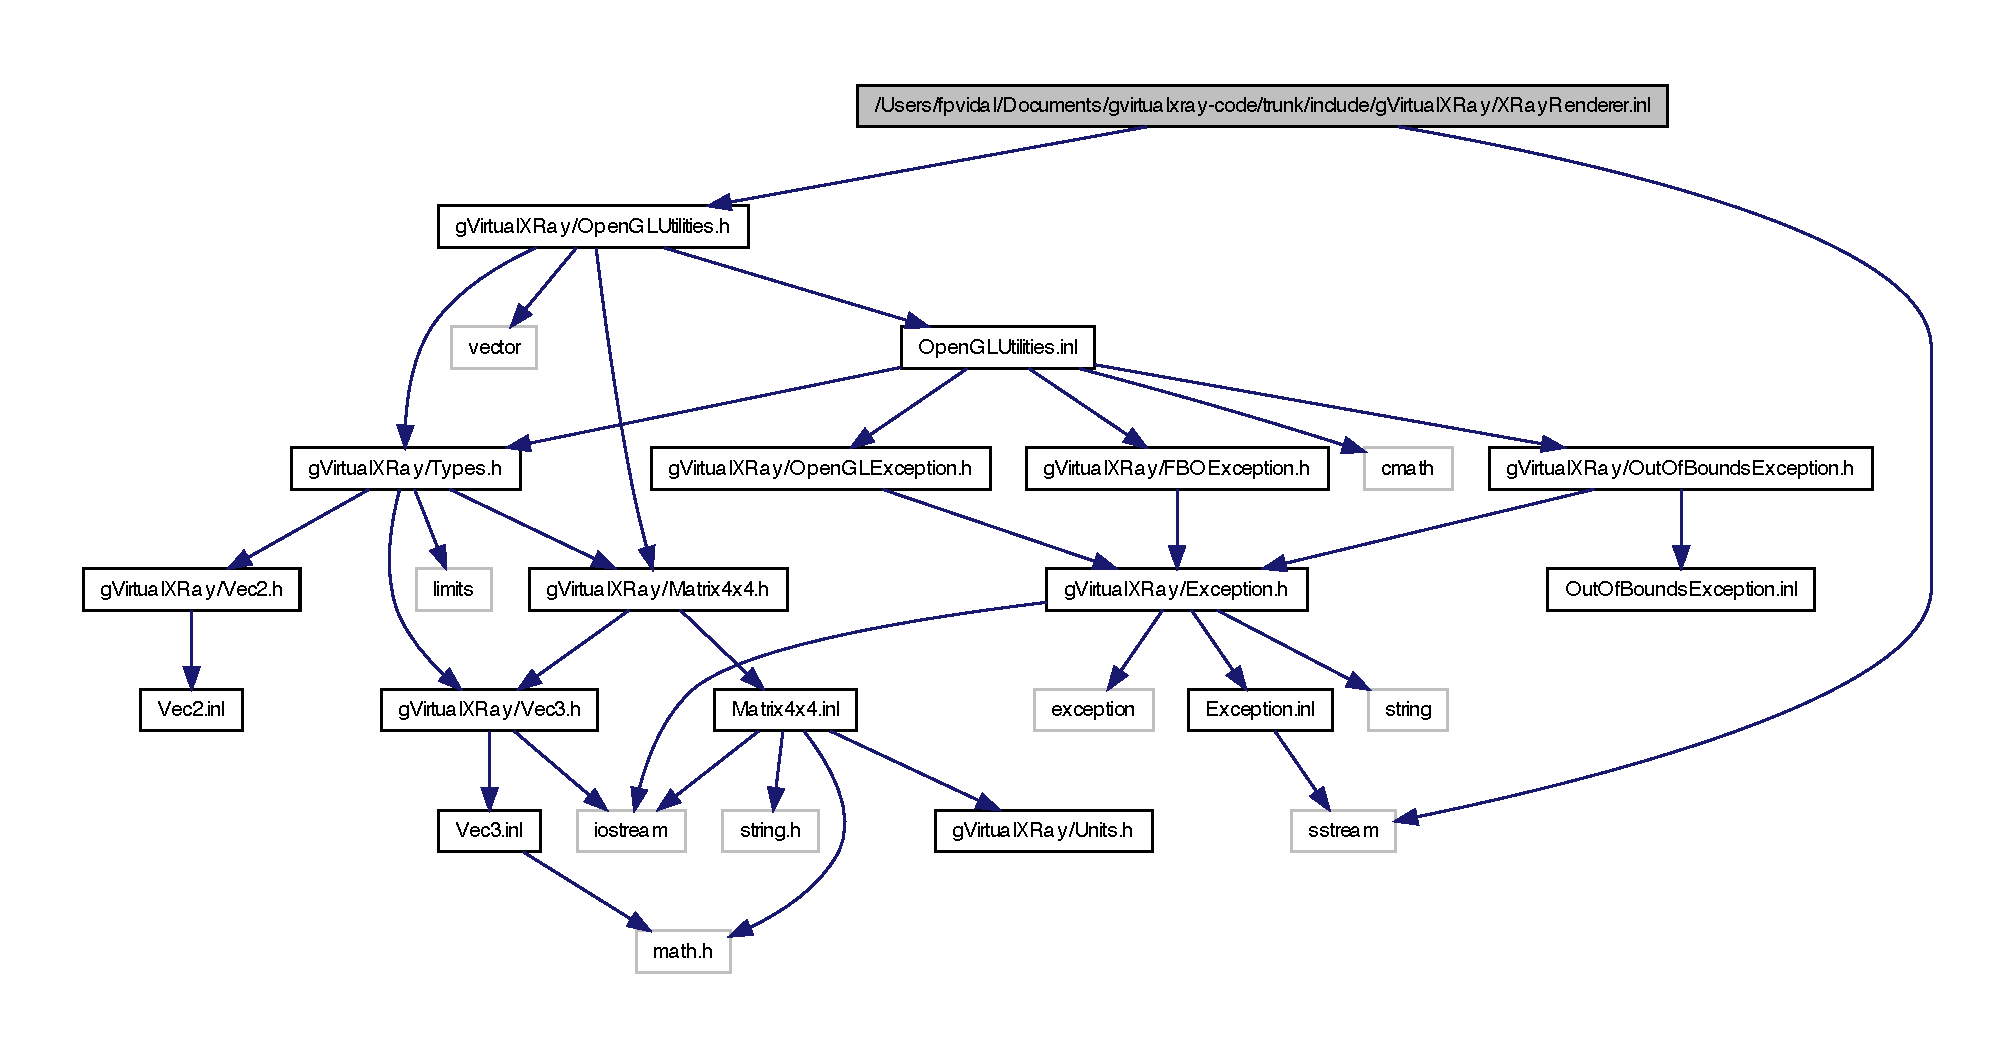
\includegraphics[width=400pt]{_x_ray_renderer_8inl__incl}
\end{center}
\end{figure}
This graph shows which files directly or indirectly include this file:\nopagebreak
\begin{figure}[H]
\begin{center}
\leavevmode
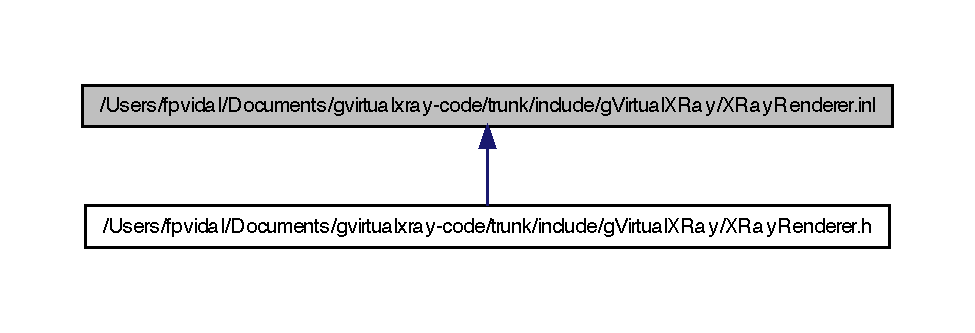
\includegraphics[width=400pt]{_x_ray_renderer_8inl__dep__incl}
\end{center}
\end{figure}
\subsection*{Namespaces}
\begin{DoxyCompactItemize}
\item 
namespace \hyperlink{namespaceg_virtual_x_ray}{gVirtualXRay}
\end{DoxyCompactItemize}


\subsection{Detailed Description}
Class to compute and renderer X-\/ray images on GPU. \begin{DoxyVersion}{Version}
1.0
\end{DoxyVersion}
\begin{DoxyDate}{Date}
01/12/2013
\end{DoxyDate}
\begin{DoxyAuthor}{Author}
Dr Franck P. Vidal
\end{DoxyAuthor}
\hypertarget{_x_ray_renderer_8inl_License}{}\subsection{License}\label{_x_ray_renderer_8inl_License}
BSD 3-\/Clause License.

For details on use and redistribution please refer to \href{http://opensource.org/licenses/BSD-3-Clause}{\tt http://opensource.org/licenses/BSD-\/3-\/Clause}\hypertarget{_x_ray_renderer_8inl_Copyright}{}\subsection{Copyright}\label{_x_ray_renderer_8inl_Copyright}
(c) by Dr Franck P. Vidal (\href{mailto:franck.p.vidal@fpvidal.net}{\tt franck.p.vidal@fpvidal.net}), \href{http://www.fpvidal.net/,}{\tt http://www.fpvidal.net/,} Dec 2013, 2013, version 1.0, BSD 3-\/Clause License 

Definition in file \hyperlink{_x_ray_renderer_8inl_source}{XRayRenderer.inl}.


\printindex
\end{document}
